%% ----------------------------------------------------------------
%% Thesis.tex -- main
%% ---------------------------------------------------------------- 

\documentclass[a4paper, 10pt, oneside]{memoir}
\usepackage{basilea}

\usepackage{tikz-network}
\usetikzlibrary{patterns}
\usetikzlibrary{matrix}
\usetikzlibrary{decorations.pathreplacing}
\usepackage{amsthm}
\theoremstyle{plain}
\newtheorem{theo}{Theorem}[section]
\newtheorem{defi}{Definition}[section]
\newtheorem{assu}{Assumption}[section]
\newtheorem{prop}{Proposition}[section]
\newtheorem{remark}{Remark}[section]
\newtheorem{note}{Note}[section]
\newtheorem{cor}{Corollary}[section]
\newtheorem{ques}{Questions}[section]
\newtheorem{lem}{Lemma}[section]
\newcommand{\parenv}[1]{\left( {#1} \right)}
\newcommand{\ceilenv}[1]{\left\lceil {#1} \right\rceil}
\newcommand{\mathset}[1]{\left\{ {#1} \right\}}
\newcommand{\sparenv}[1]{\left[ {#1} \right]}
\newcommand{\Prob}[1]{\mathbb{P}\!\left[{#1} \right]}
\newcommand{\Ex}[1]{\mathbb{E}\!\left[{#1} \right]}
\newcommand{\Var}[1]{\mathbb{E}\!\left[({#1} -\Ex{#1})^2 \right]}
\newcommand{\td}{\tilde{d}}
\newcommand{\eqdef}{\triangleq}
%% ----------------------------------------------------------------
\begin{document}

% for english use \selectlanguage{english}, for german use \selectlanguage{ngerman}
\selectlanguage{english}

\thesisfront
\maketitle
\pagestyle{thesis}
%% ----------------------------------------------------------------
%%%\chapter*{Dedication}
\begingroup
\patchcmd{\chapter}{\thispagestyle{plain}}{\thispagestyle{empty}}{}{}
\chapter*{} % Hidden chapter title
\addcontentsline{toc}{chapter}{Dedication} % Add chapter to table of contents
\endgroup


\begin{center}
     To my family and closest friends for their unwavering support and constant encouragement throughout all my personal and professional adventures.
\end{center}

\addcontentsline{toc}{chapter}{Declaration of Originality}
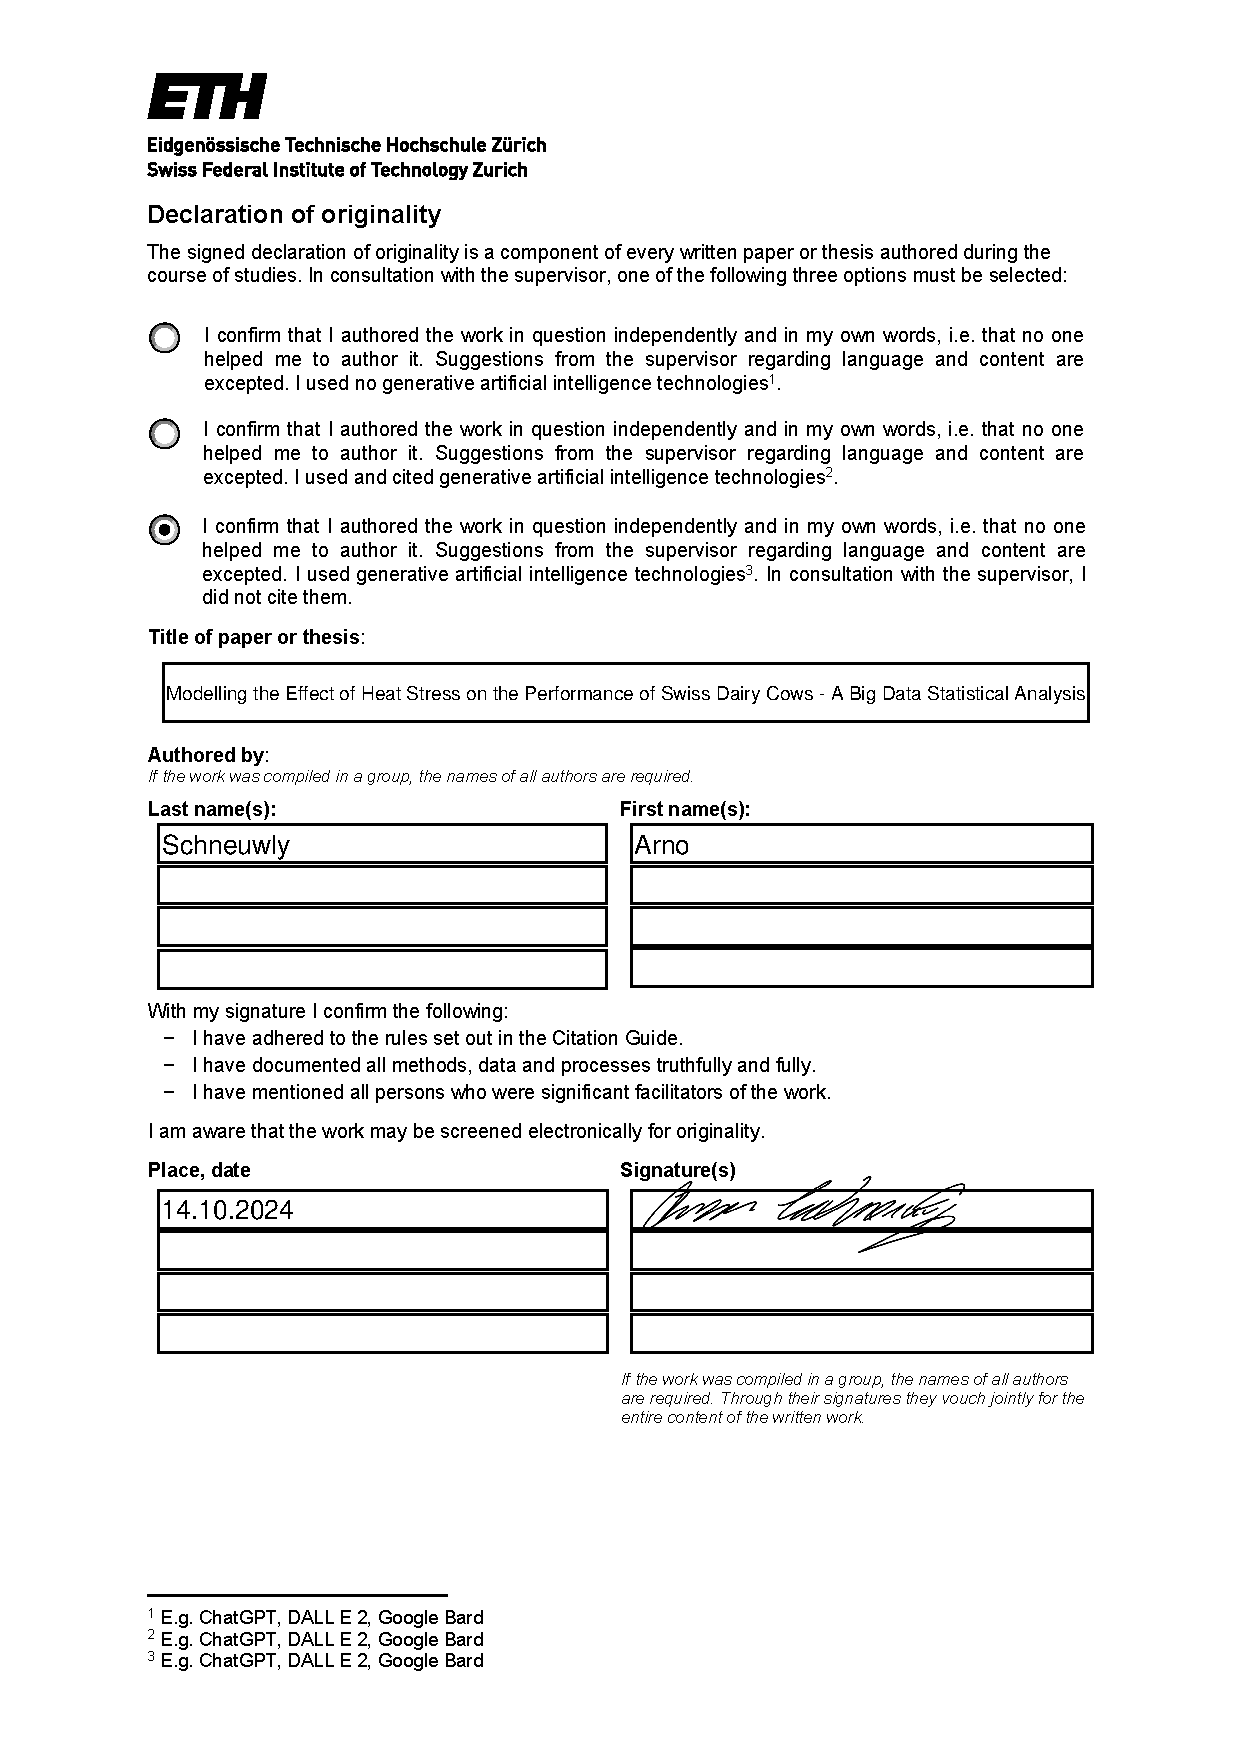
\includepdf[pages=-]{front/declaration-originality_signed_flattened.pdf}
%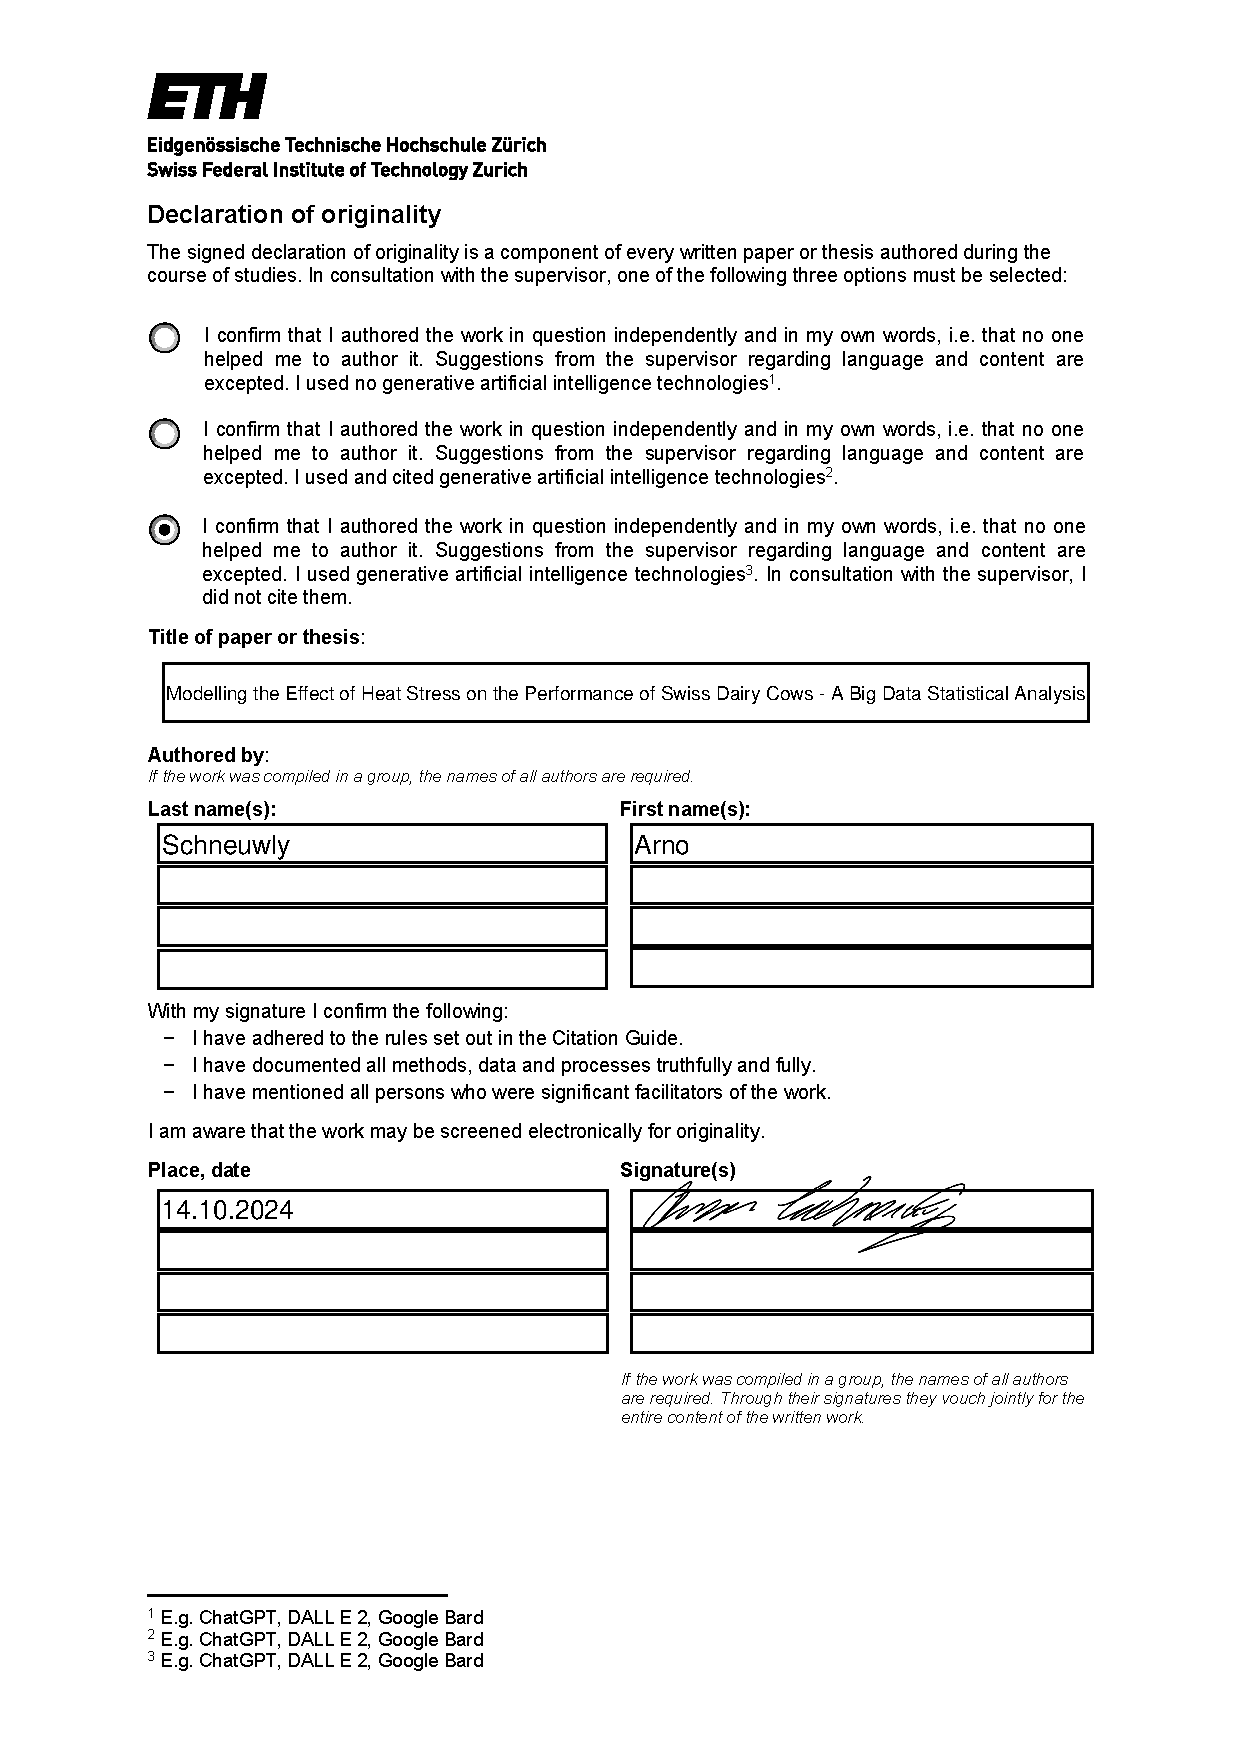
\includepdf[pages=-, pagecommand={\thispagestyle{fancy}}]{front/declaration-originality_signed_flattened.pdf}
\chapter{Project Description}
\section*{Project Title}
Impact of climate change on the landscape of the dairy sector in Switzerland over the past decades

\section*{Description}

Climate change, as a consequence of anthropogenic greenhouse gas emissions and global population growth has become major challenge for humanity. The global increase in temperature and humidity amplifies local impact on livestock husbandry. Heat stress (HS) is defined as body hyperthermia in mammals due to excessive heat loads that cannot be sufficiently dissipated. Modern dairy cows are more susceptible to HS due to higher metabolic activity during lactation compared to other animals.

\vspace*{\baselineskip}
Based on projected growth in the human population, the global food demand is estimated to increase by 60 to 70\% by 2050 \citep{makkar_review_2018}, of which the demand for dairy products is greater than 50\% compared to the values of 2010 \citep{fao_world_2011}. Seasonal depression in milk production is mainly attributed to HS, and thereby increasing global temperatures represent a challenge to meet the growing demand for dairy products, as higher ambient temperature and humidity reduce the production efficiency of dairy cows. Climatic conditions around the world vary because animals live in a combination of environmental factors, including humidity, rainfall, wind speed, and solar radiation \citep{johnson1987}. The temperature-humidity index (THI) was proposed to represent the combined effects of ambient temperature and relative humidity associated with HS \citep{national1976livestock}. Heat stress is considered an acute effect on dairy cows when THI crosses the threshold of 72 \citep{armstrong_heat_1994} or 68 \citep{de_rensis_seasonal_2015}.

\vspace*{\baselineskip}
Heat stress causes significant economic losses to the livestock sector \citep{key_climate_2014}. For example, estimated losses in the U.S. range from \$ 1.7 to 2.4 billion, of which \$ 0.9 billion are specific to the dairy sector \citep{st-pierre_economic_2003}. Even in a temperate climatic region, such as Central Europe, dairy cows are greatly affected by seasonal exposure to heat \citep{fabris_effect_2019}. Although such financial estimates are currently not available in Switzerland, our analysis showed reductions in milk yield (MY) and milk fat and protein contents in Swiss dairy farms during the summer months, translating into significant losses in dairy food quality, nutrients, and farm sustainability (Fig.~\ref{fig:niu_annual_seasonality}).

\begin{figure}[H]
    \centering
    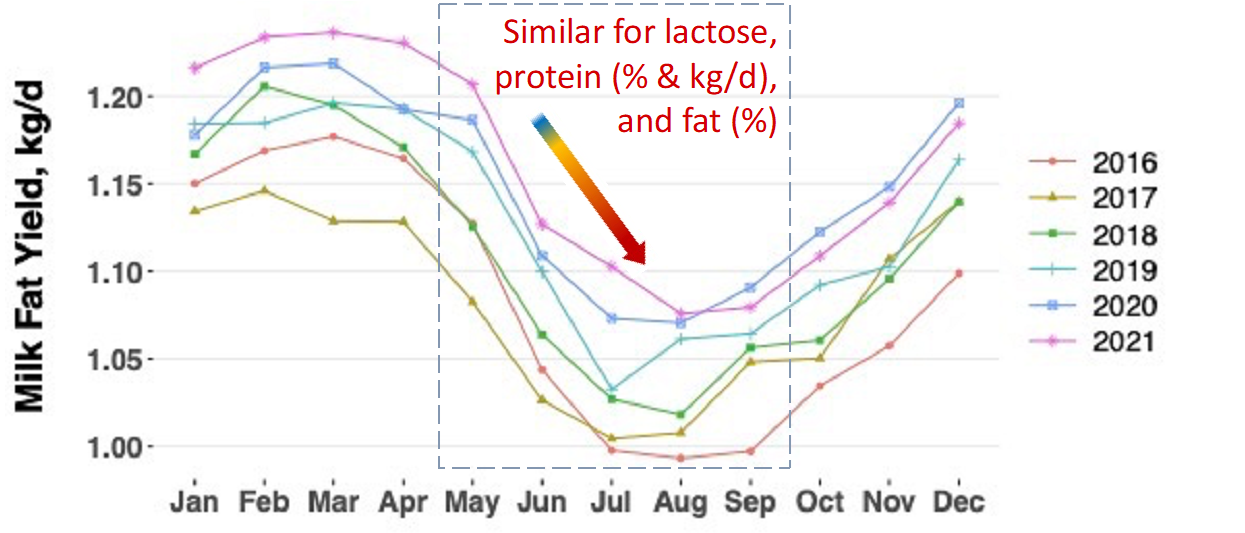
\includegraphics[width=0.7\textwidth]{./thesis/figures/project_description.png}
    \renewcommand{\thefigure}{A}
    %\captionsetup{list=false}
    \caption{Based on a total of 2'090'000 test day records from Swissherdbook, Niu et al., (unpubl.) analyzed milk fat yield of cows in registered Swiss dairy farms during 6 consecutive years across the annual cycle.}
    \label{fig:niu_annual_seasonality}
\end{figure}

Hence, our objective is to analyze, with appropriate methods, extreme weather effects on the quantitative and qualitative aspects of the dairy business in Switzerland with an unprecedented granularity level. The analysis should be performed on cow- or farm-level datasets. In addition, meteorological data from MeteoSwiss \citep{meteoswiss} allow us to investigate potential relationships between parameters at the cow level, the farm level, and the HS factors. Ideally, the work will provide valuable insights for the dairy industry, policy makers, insurances, and other stakeholders in the Swiss dairy value chain.

%\chapter*{Dedication}
\begingroup
\patchcmd{\chapter}{\thispagestyle{plain}}{\thispagestyle{empty}}{}{}
\chapter*{} % Hidden chapter title
\addcontentsline{toc}{chapter}{Dedication} % Add chapter to table of contents
\endgroup


\begin{center}
     To my family and closest friends for their unwavering support and constant encouragement throughout all my personal and professional adventures.
\end{center}
\chapter{Acknowledgments}

\textit{Zurich, Switzerland - October 2024}

\vspace*{\baselineskip}
First and foremost I would like to thank Mutian Niu and Usman Arshad for hosting me in the Animal Nutrition Group at Strickhof and providing excellent guidance throughout the past months to enable steady progress in our interdisciplinary project despite unforeseen hurdles with the sparsity of our data. Moreover, I also express my gratitude to Boris Zandona, Meiqing Wang and Elli Broxham Stahl for accommodating all my side requests regarding logistics and infrastructure.

\vspace*{\baselineskip}
Furthermore, this work could not have been realized without the generous support of Adrien Butty (Qualitas AG), Nicolas Berger (Swiss Herdbook), Martin Rust (Braunvieh Schweiz) and Timothée Neuenschwander (Holstein Schweiz) who granted access to the full database of day milk samples collected by Swiss dairy cow breeding associations over the past 40 years. In addition, I extend our appreciation to Peter Molnar from the ETH Chair of Hydrology and Water Resources Management for generously providing access to gridded weather data.

\vspace*{\baselineskip}
I would also like to thank Paul Rosenfield from Farmers Business Network who instructed and unblocked us with his in-depth knowledge in Generalized Additive Mixed Models with respect to the particular structure of our data. Without him we would probably not have been able to retrieve any meaningful results in such a short time horizon. In addition, Lukas Graz from the Consulting Service at the ETH Seminar of Statistics also provided valuable feedback for our questions. On top of that, I wish to acknowledge the insightful conversation with Laurence Jungo from Suisselab AG, who provided valuable insights regarding the history and methods of milk sampling in Switzerland.

\vspace*{\baselineskip}
Last but not least, I would like to thank Emma Lindberg, Brigitte Dorn, Maria Rey, and Emmanuel Frossard - the study administration of the Institute of Agricultural Sciences at ETH - for their support over the past years.
%% ----------------------------------------------------------------
\chapter{Abstract}
Climate change is increasingly contributing to higher average temperatures which lead to frequent and severe heat waves across the globe. These shifts can intensify heat stress in dairy cows and might adversely affect milk production and component yields. However, the degree of heat tolerance among dairy cow breeds has not been extensively studied in commercial production settings within Switzerland. Existing research has largely focused on a limited number of breeds in grassland-based systems outside of Switzerland. Using a comprehensive dataset comprising over 130 million records from the three major dairy cow breeding associations in Switzerland, we investigated the effect of weather on milk yield and energy-corrected milk yield across six dairy cow breeds, providing an unparalleled analysis in terms of scale and scope.

\vspace*{\baselineskip}
We employed Generalized Additive Mixed Models (GAMMs) to adequately model the non-linear Temperature Humidity Index (THI) and other variables such as days in milk (DIM). This required us to develop a modified implementation of \textit{gamm4 (R)} and \textit{MixedModels.jl (Julia)} adapted to the sparse structure of our dataset. With these modifications, we enabled GAMMs to accommodate a larger number of random effect factor levels than previous implementations in \textit{R} while enhancing computational efficiency.

\vspace*{\baselineskip}
Applying this tailored method to our model, we determined the marginal non-linear effects of THI on the daily milk yield and the daily energy-corrected milk (ECM) yield for both primiparous and multiparous cows. We retrieved breed-specific THI response curves and peak performance points. Our results indicated that dairy performance decreased at three-day mean THI values as low as 51 for certain breeds, which was notably lower than reported in comparable studies. Furthermore, we observed greater variability in peak THI values for milk yield across breeds compared to ECM yield, suggesting that high-fat and high-protein-producing breeds such as Jersey experience earlier declines in milk component yields. Across all scenarios, primiparous cows consistently showed lower heat tolerance compared to multiparous cows. Furthermore, when the data was divided into periods before and after 2010, lower peak THI values were observed in the latter period, possibly indicating a decline in heat tolerance due to breeding practices.

\vspace*{\baselineskip}
Despite substantial advancements in computational capabilities enabling the acquisition of our results, we advise conducting additional statistical validation employing techniques such as bootstrapping, cross-validation, or alternative subsampling strategies. Furthermore, to statistically consolidate the findings, consideration may be given to a multi-breed model that integrates all dairy cow breeds into a single unified model. Some of these steps would require additional algorithmic optimizations. Nonetheless, the rich dataset available presents opportunities for further research, including the examination of additional milk performance parameters such as lactose content or somatic cell count. Also, incorporating the animal breeding history into the model could provide deeper insights into breeding dynamics and effects on heat responses. The consideration of pre-calving weather exposure also warrants attention. Moreover, the low peak-performance THI values in our results highlight the necessity of future studies on heat stress mitigation strategies, for instance, through dietary interventions.

%% ----------------------------------------------------------------
\thesistoc
%% ----------------------------------------------------------------
\clearpage
\listoffigures
\clearpage
\listoftables
%\thesisnomencl
%% ----------------------------------------------------------------
\thesismain
\chapter{Introduction}\label{chap:introduction}
 Climate change leads to higher average and daily maximum temperatures as well as a more frequent occurrence of heat waves \citep{meteoschweiz_klimaindikatoren_2024, ipcc_2023}. For example, summers in Switzerland during 2023, 2022, 2019, 2018, 2017, and 2015 have demonstrated a marked increase in the frequency of prolonged periods of high temperatures \citep{heatwaves_switzerland}. Figure~\ref{fig:number_of_hot_days} depicts this trend.

  \begin{figure}[H]
    \centering
    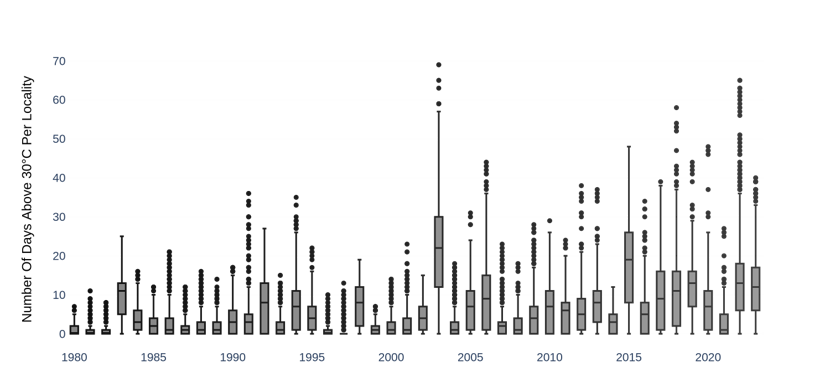
\includegraphics[width=\textwidth]{thesis/figures/number_of_hot_days_switzerland.png}
    \caption{Annual frequency distribution of hot days in all localities within Switzerland since 1980, where a hot day is characterized by a maximum temperature exceeding 30°C.}
    \label{fig:number_of_hot_days}
\end{figure}
 
 These unfavorable weather conditions are detrimental to agricultural production. For dairy farmers, elevated temperatures can adversely affect milk yield, quality, fertility, and other related factors \citep{bernabucci_effect_2015,lambertz_climatic_2014, bohmanova_temperature-humidity_2007, dunn_analysis_2014,ranjitkar_will_2020, west_effects_2003, gantner_differences_2017,maggiolino_estimation_2020,salfer_annual_2019,smith_short_2013,hammami_evaluation_2013,hill_dairy_2015, vitali_effect_2015, cox_mortality_2016}. 
 The magnitude of the effects of heat stress on dairy milk production varies across breeds and has been analyzed for a subset of breeds and geographic regions outside of Switzerland \citep{bryant_quantifying_2007, smith_short_2013, gantner_differences_2017, ahmed_temperature_2022}. Although the dairy sector represents the largest share of the national agricultural production, accounting for 23\% of total output with over 545'000 cows \citep{agrarbericht_2023}, the extent to which dairy producers are exposed to quantitative and qualitative milk losses for different breeds remains uncertain. According to the Swiss Federal Office of Agriculture the agricultural production should be adapted to climate and regional properties. In line with this objective, this work provides an assessment on how hot weather impacts the milk quantity and quality in Switzerland. In particular, we examine how milk yield (MY) and energy-corrected milk yield (ECM) are affected by varying levels of the Temperature Humidity Index (THI). Acknowledging that previous studies indicate diverse coping mechanisms with heat stress among breeds, this research emphasizes a comparative analysis of multiple breeds. To facilitate this investigation, we utilize subsamples from a dataset comprising 130 million test-day samples sourced from the three principal breeding organizations in Switzerland. These samples span a period of 42 years, from 1982 to 2023, with data from six predominant breeds: Holstein, Brown Swiss, Original Braunvieh, Swiss Fleckvieh, Simmental, and Jersey. The dataset covers the entire national territory.



\section{Literature Review}
\paragraph{The Effect of Heat Stress Across Dairy Cow Breeds} \quad \\
\textit{Different breeds have different responses to heat stress with respect to milk production. The impact of heat stress while making a distinction between breeds is globally understudied.}

The majority of studies assessing the impact of heat stress on the performance of dairy cows focus on a single breed, with examples such as \cite{bernabucci_effect_2015, lambertz_climatic_2014,hammami_evaluation_2013, hill_dairy_2015}. Only a limited number of authors consider multiple breeds. According to \cite{bryant_quantifying_2007}, Holstein Friesians exhibit greater sensitivity to heat effects compared to New Zealand Jerseys, with the latter maintaining a more stable milk yield under elevated 3-day mean THI conditions. No significant differences were observed in protein and fat content between the two breeds. \cite{smith_short_2013} report an increase in milk production among Jersey cows during heat stress, while performance declines for Holsteins in a research farm in the United States. \cite{gantner_differences_2017} explore the milk performance of Holstein and Simmental cows in Croatia, finding a greater vulnerability to heat stress among high-producing cows compared to their low-performing counterparts. Their findings suggest a higher resistance to heat stress in Simmental breeds compared to Holsteins, though further research is warranted. \cite{ahmed_temperature_2022} examine the effects of heat shocks—defined as periods of five consecutive days with average temperatures exceeding 25°C—on milk production. Overall, no significant differences in heat shock tolerance were observed among Swedish Holsteins, Swedish Reds, and a crossbreed of the two in Sweden, suggesting that breed diversification as a strategy to mitigate heat stress risks is ineffective. Nonetheless, Swedish Red cows exhibit greater resilience to negative heat effects when considering heat events in relation to the genetic milk index. \cite{cuellar_differences_2023} include Brown Swiss in a comparative study with Holsteins and their crossbreeds, finding a more pronounced decrease in milk yield for Brown Swiss than for Holstein. 

\paragraph{The Effect of Heat Stress in Swiss Dairy Production} \quad \\
\textit{The effect of heat stress on the quantity and quality of milk production at the animal-level for commercial farms in grassland-based systems over a long period of time is understudied in Switzerland.}

Globally, the phenomenon of heat stress in dairy cows is extensively researched, particularly at the level of individual animals in research farms. Additionally, numerous studies have quantified the effects of heat stress on dairy cows using panel data across various regions worldwide. The works mentioned in the preceding paragraph represent only a select number of these investigations. Only a few recent studies consider data from Switzerland to study the effects of heat stress on dairy cows: \cite{bucheli_heat_2022} analyze the annualized farm-level effect of heat stress on milk revenues, veterinary expenses and feed purchases. In the period from 2003 to 2015 Swiss farmers are on average financially robust to heat exposure. However, this does not imply non-existence of a related risk. \cite{gasser_can_2023} find that meteorological features do not improve the accuracy of daily milk yield predictions. The data originates from an experimental farm in Tänikon, Switzerland. Furthermore, \cite{holinger_behavioural_2024} observe behavioral changes in cows under heat stress with data of four Swiss commercial farms in the period from June to September 2021. During days characterized by elevated maximum THI values, cows are observed more frequently in proximity to the drinker during the morning hours. In contrast, during the afternoon, they tend to congregate in close proximity to each other and seek shade. Moreover, on such days, there is a notable decrease in the duration of time spent lying down, accompanied by an increase in their locomotor activity as noon approaches.

\section{Research Objective}
This study seeks to build upon methodologies established in prior research to examine the impact of heat stress on Swiss dairy production across various breeds. Although the complex physiological responses of individual animals to heat stress are extensively studied and well documented \citep{kadzere_heat_2002,becker_invited_2020}, the effects of heat stress at broader geospatial scales, including herd, regional, and national levels in grassland-based systems across breeds, remain under-researched. Swiss dairy farms predominantly employ pasture-based systems, with cows spending substantial amounts of time grazing outdoors \citep{agrarbericht_2023}. Evaluating the effects of THI on milk performance variables within this production context could provide valuable insights into the actual influence of ambient temperature and humidity on dairy cows.

\vspace*{\baselineskip}
Heat stress exerts a direct impact on economically significant factors, including milk yield, milk component yield, and the health of cows. For dairy farmers, variations in the quantity and quality of production are anticipated and regarded as standard to some degree. Nevertheless, these agronomic factors are intrinsically connected to the dairy producers' revenue streams from milk. Farmers continuously modify their management practices, generally through technological advancements, enhanced knowledge, or shifts in policy \citep{agrarbericht_2023, koutouzidou_evolution_2022}, as well as in response to heat stress \citep{ji_review_2020,vroege_effects_2023}. This includes, for example, feeding regimes, housing systems, cooling systems, milking technologies or breeding strategies \citep{kadzere_heat_2002, west_effects_2003}. All these potentially confound heat stress effects and pose obstacles for a full isolation of the causal weather effects.

\vspace*{\baselineskip}
Switzerland is a topologically diverse country. This geographic variability leads to different heat exposures on a regional level as depicted on Figure~\ref{fig:thi_80}. The effective animal-level heat exposure depends on many environmental factors. In our work, our aim is to develop a framework to isolate the weather effects from farm-specific properties, spatial heterogeneity, herd characteristics, as well as individual animal responses and assess their impact on the aforementioned agronomic indicators. Moreover, we specifically check for weather effect differences across breeds to validate if certain breeds are more-heat stress tolerant than others and may qualify for heat-stress resilience under the warming climatic trends in Switzerland. Our analysis remains at the breed level and does not consider genomic selection or herd evolution.

\begin{figure}[H]
    \centering
    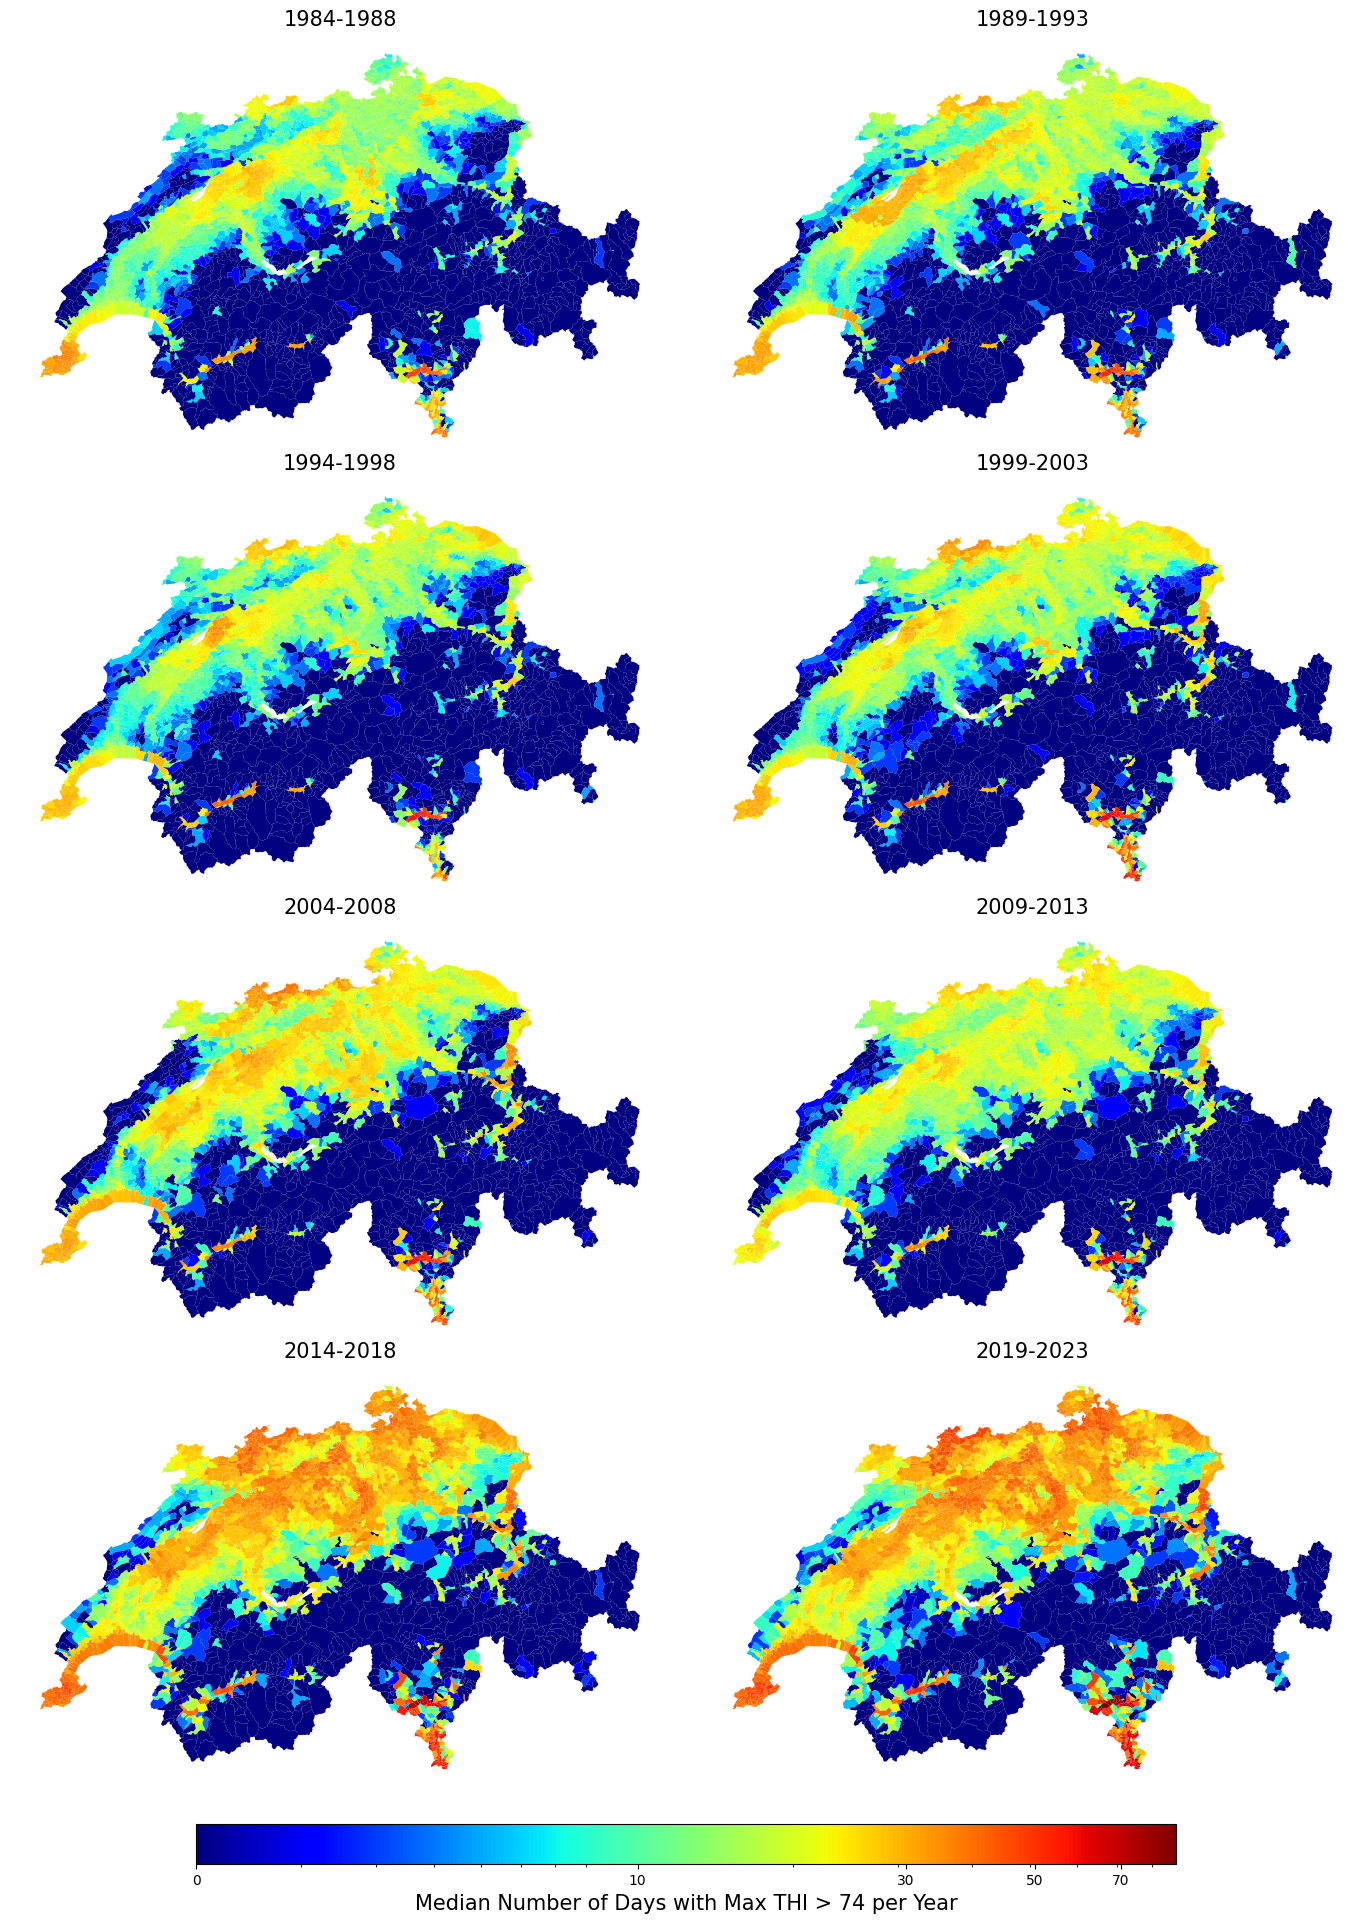
\includegraphics[width=\textwidth]{figures/00_thi_above_80/thi_above_74.png}
    \caption{The median number of days when the maximum THI surpasses the threshold 74 substantially increases for some regions in the period $t_1$ from 1984 to 2023. A THI of 74 stands for moderate heat stress. The coloring scheme is logarithmic because some towns in the canton Ticino (southermost part) exceed the median compared to the rest of Switzerland considerably. Moreover, dairy farming is more widespread in the northern parts of Switzerland.}
    \label{fig:thi_80}
\end{figure}

\section{Research Question and Hypothesis}\label{sec:research_question}
To achieve the above-mentioned objective, the study sets the main focus on the following research question:

\begin{center}
    \textit{At what Temperature Humidity Index (THI) values do changes in dairy performance occur for the different dairy cow breeds in Switzerland?}
\end{center}

The primary variables under consideration are the milk yield, measured in kilograms per day, and the energy-corrected milk yield (ECM), also measured in kilograms per day. The ECM incorporates yields from both fat and protein components. Recognizing the variance in component yields across different breeds, the ECM yield provides a standardized measure for comparative analysis among breeds. Building upon previous studies, it is anticipated that both volumetric and component yields will decline once specific thresholds of the Temperature-Humidity Index (THI) are surpassed. Reported threshold values include 68 \citep{de_rensis_seasonal_2015}, 72 \citep{armstrong_heat_1994}, and 76 \citep{vroege_effects_2023}\footnote{Many studies employ differing definitions of THI and utilize diverse aggregation methodologies, including summation, averaging, as well as determining minimal or maximal values over hours, single days, multiple days, weeks, months, or even years. Consequently, careful consideration is imperative in the interpretation of THI values.}. It is further anticipated that there will be breed-specific variations in the THI values critical for optimal dairy performance \citep{kadzere_heat_2002}. Jerseys are posited to exhibit greater heat tolerance compared to Holsteins, a characteristic also expected in the Simmental breed. In conclusion, the Holstein breed, known for high yields, is likely to experience greater stress under increased heat conditions compared to lower-yielding breeds such as Simmental and Jersey.

\section{Organization}
The remainder of this document is organized as follows: First, in Chapter~\ref{chap:background}, we provide an overview of various aspects regarding heat stress in dairy cows, breeds, and farms to set the agronomic scope. This includes aspects from animal physiology, but also political and economic aspects of the Swiss dairy market because our study covers a time period of 42 years. Second, within Chapter~\ref{chap:material_methods}, in consideration of the non-experimental nature of our study, we delineate our data strategy along with an exploratory data analysis in Section~\ref{sec:data}. This examination incorporates the agronomic, the meteorological, and the geospatial data. Guided by our research question and the insights gained from the data analysis, we determine the appropriate model and estimation strategy in Section~\ref{sec:models} and Section~\ref{sec:estimating_gams}. This includes our methodological advancement to estimate Generalized Additive Mixed Models with an unprecedented number of random effect factor levels. Third, we analyze and discuss the findings in Chapter~\ref{chap:results}. The concluding Chapter~\ref{chap:conclusion} summarizes our contributions, limitations, and also proposes future research directions.
\chapter{Background}\label{chap:background}
At a high level, the production of dairy farming and livestock can be expressed as the result of a phenotype product $P$ which is a combination of a genotype $G$ realization and environmental factors $E$: $P = G + E + G \times E$ \citep{adhikari_climate_2022}. The genetic factors $G$ are influenced by breeding. The environmental factors $E$ are farm management practices such as housing or feeding, policy and socio-economic environment, ambient weather and climate. Both breeding strategies and changing environmental conditions impact susceptibility to heat stress, dairy performance, animal health and reproduction. The interaction between the G and E determines to which degree a dairy cow may express the full genetic potential with respect to a selected metric such as milk performance.

\vspace*{\baselineskip}
Given the animal-level nature of our dataset, this chapter starts with an overview of the physiological aspects of dairy cows under heat stress conditions in Section~\ref{sec:animal_physiology}. We thereby highlight critical factors that may necessitate modelling. Then, in Section~\ref{sec:breed_models} we analyze a range of selected models estimating heat-effects across breeds to appraise the current technical state-of-the art and identify potential gaps. This is followed by a comprehensive review of the developments in Swiss milk production over the past four decades in Section~\ref{sec:evolution_market}, aligning with the scope of our data: breeding associations set long-term goals which ideally increase the milk yield in the long run. Moreover, legislative amendments and policy measures can substantially influence farm management practices and breeding techniques. Collectively, this chapter establishes the foundational understanding of factors that may inform the modeling process in Chapter~\ref{chap:material_methods}.

\newpage

\section{Animal Physiology}\label{sec:animal_physiology}
This section summarizes key concepts in animal physiology pertaining to heat stress. Unless explicitly indicated otherwise, the review from \cite{kadzere_heat_2002} serves as the source of information for this section and its subsequent subsections. We discuss some aspects of the cow physiology to better understand the complex heat-related interactions between the animal $G$ and the environment $E$. Moreover, the section highlights physiological arguments, why we might expect different heat stress responses for different breeds.


\begin{figure}[ht]
    \centering
    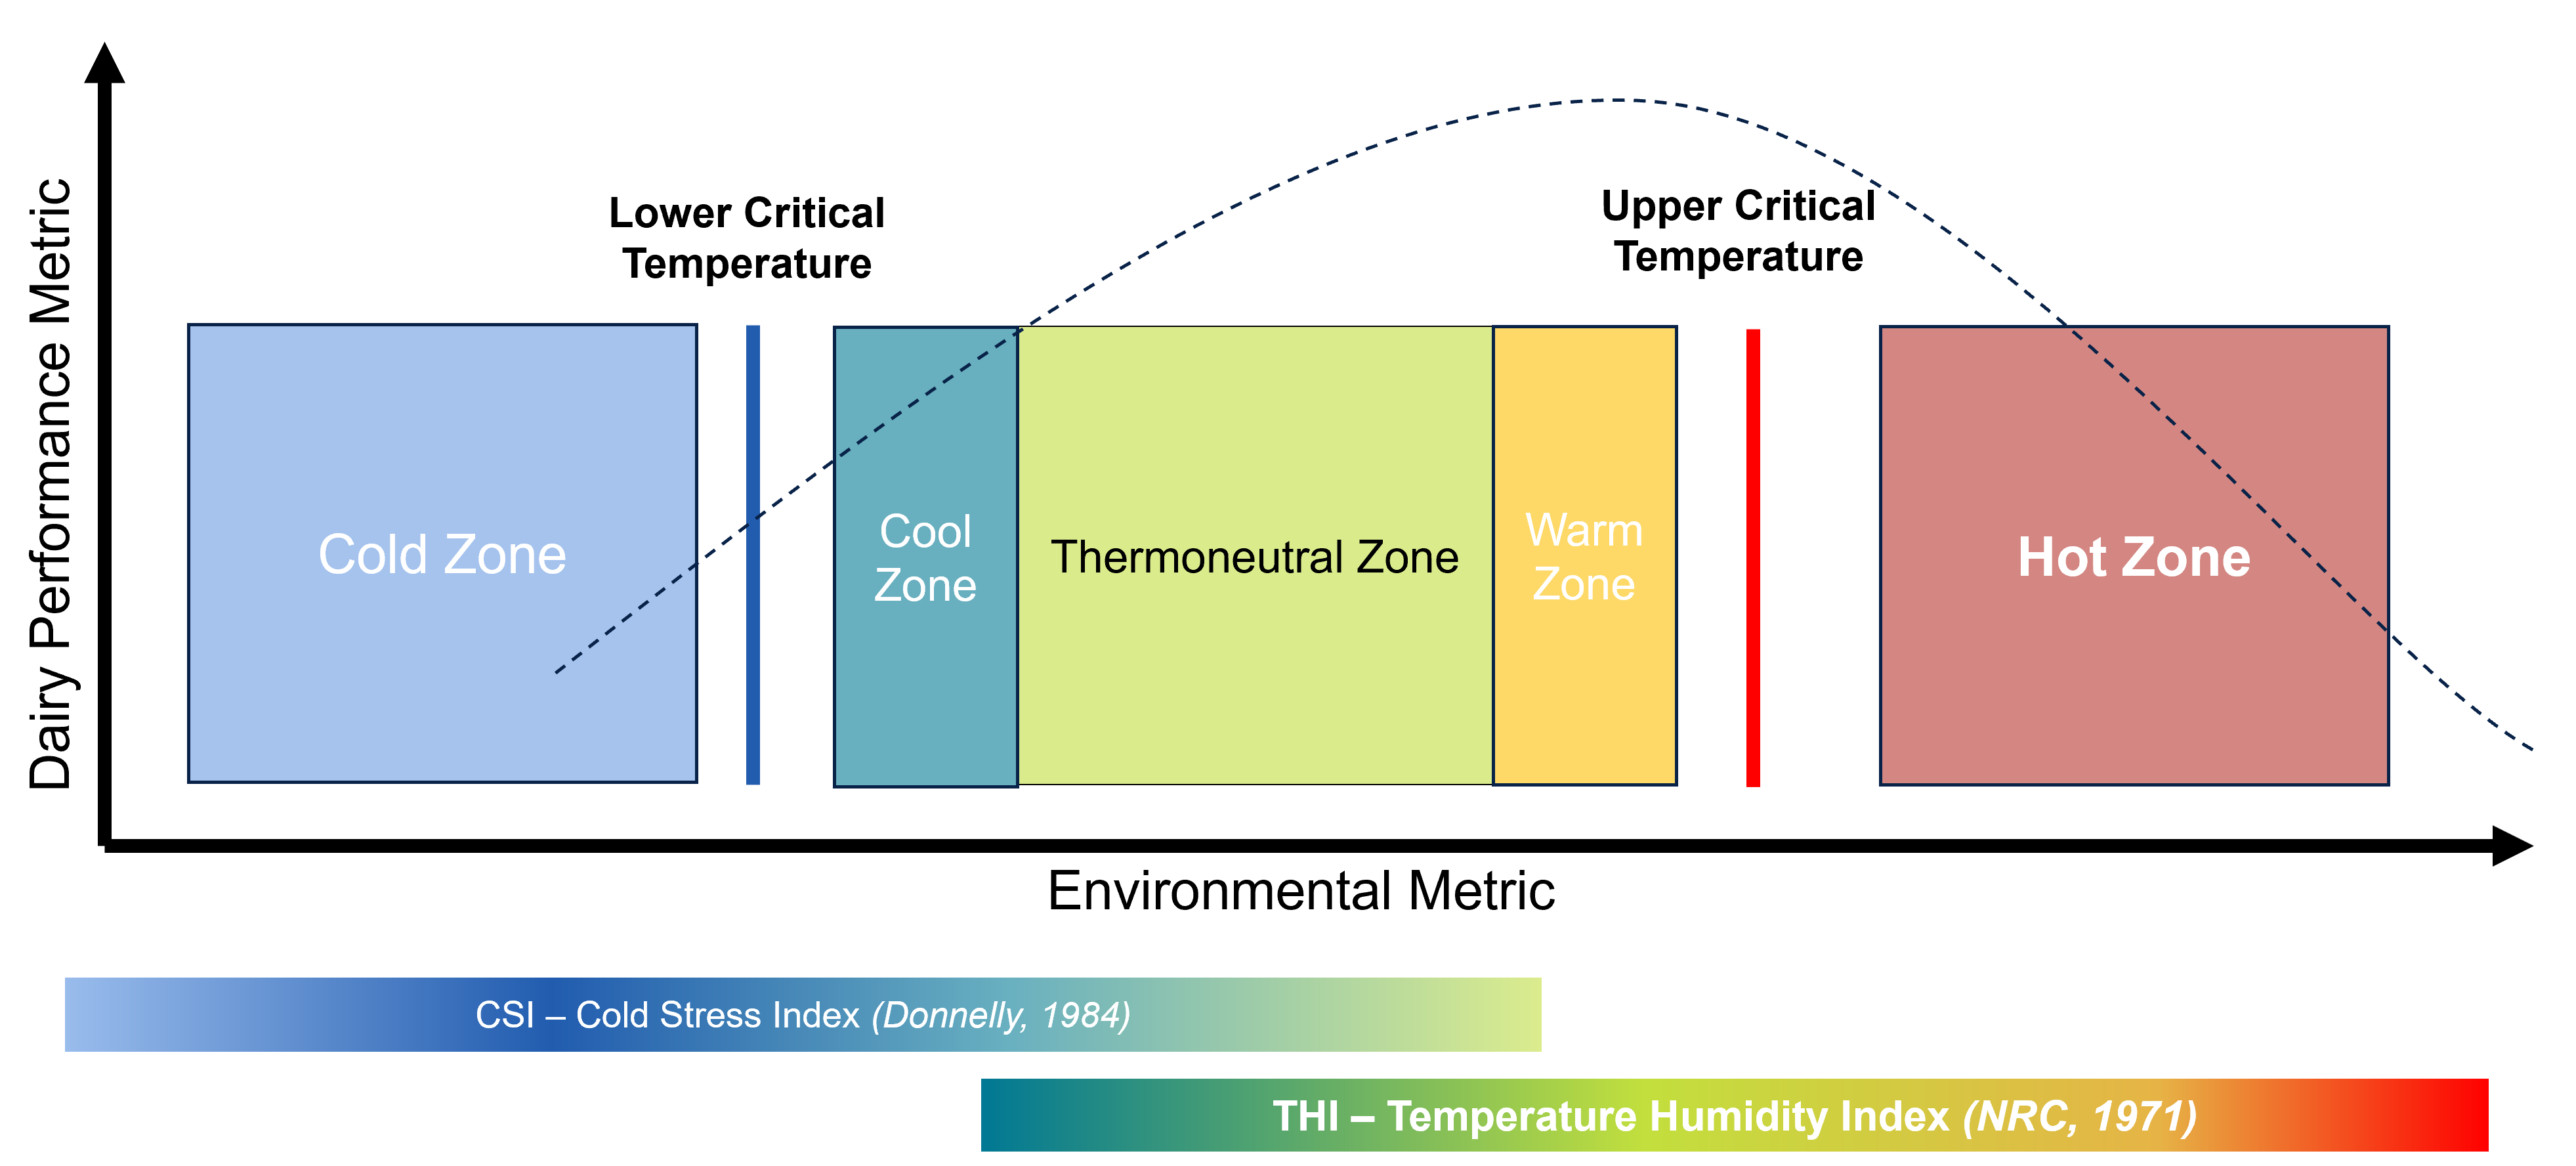
\includegraphics[width=\textwidth]{thesis/figures/physiology.png}
    \caption{Animal physiology: a dairy cow achieves maximum productivity at minimal physiological costs in the thermoneutral zone. A broadly accepted environmental metric to measure heat stress is the Temperature Humidity Index (THI).}
    \label{fig:ainmal_physiology}
\end{figure}

\vspace*{\baselineskip}
\begin{defi} Heat Stress in Dairy Cows \\
    Heat stress is the collective impact of high temperatures compelling adjustments from sub-cellular to the whole animal level in order to avoid a physiological dysfunction and adapt better to the current environment. 
\end{defi}

As a homothermal the cow must maintain a thermal equilibrium with the environment to regulate the biochemical reactions and physiological processes. The environmental factors include air temperature, air movement, humidity, as well as radiation. When cows fail to balance their body temperature within their thermoneutral zone and keep it in physiological homeostasis, they will experience hyperthermia, which may lead to death. The main characteristics of heat stress, independent of any effects of feed intake, are elevated respiration rates, increased rectal temperatures, an impaired metabolism, reduced growth and lactation, as well as poor reproductive performance.

\subsection{Thermoregulation}\label{sec:thermoregulation}
\paragraph{Heat Increment}
The heat production in the dairy cow serves to maintain equilibrium with heat dissipation mechanisms and is controlled by the nervous system, endocrine system, appetite, digestion, respiratory enzymes as well as protein synthesis. Factors affecting the heat production intensity are the ambient temperature, hormone concentrations such as growth hormones, body size, breed, fodder and water availability. Heat increment is the increase in body heat production resulting from digestation, heat absorption and the metabolism of nutrients activated through feed intake. Large amount of feed intake generate significant metabolic heat. Moreover, an increased milk production relates to a raised heat increment. The heat increment during the lactogenesis depends on the fodder quality and quantity. The milk production capacity also depends on the cow size. The latter is linked to the size of their gastrointestinal tracts, which have bigger digestion capacity in larger cows. This increased capacity results in a higher substrate availability for the milk production. 

\paragraph{Heat Dissipation}
Dairy cows lose heat through factors such as sweating, changes in environmental temperature, changes in the radiating surface, air flow changes, or convection. The amount of radiant heat a cow absorbs is influenced by the environmental temperature and its coat color. Dark-coated cows, for instance, generally absorb more heat than those with lighter brown coats. Cows can release metabolic heat through evaporative cooling, wherein water absorbs heat from the cow's surface. The degree of heat loss through evaporation rises with increasing ambient temperatures. Additionally, convection serves as a method for heat dissipation when cooler air circulates around the warmer body, absorbing heat which is then carried away. However, if the surrounding air is warmer than the cow's skin, heat is instead transferred into the animal's body. Conductive transfer, another form of heat exchange, happens when the cow is in direct contact with another surface or entity. Unlike convection, which entails the movement of the subject, conduction involves heat transfer without the displacement of the subject. Conduction becomes pertinent when a cow is lying down, thus selecting appropriate ground surfaces or bedding materials is important for both animal welfare and strategies to mitigate heat stress.

\paragraph{Thermoneutrality}
Overall, the maintenance of thermoneutrality requires an equilibrium between heat gains and heat losses with the environment. This can be stated with the following heat balance equation $M = \pm K \pm C \pm R + EV$, where $M$ is the metabolic heat production, $K$ is the heat exchanged by conduction, $C$ by convection, $R$ by radiation, and $EV$ by evaporation. Generally, the thermoregulatory response of dairy cows may have changed over time since breeding strategies promote a genetic selection for an increased milk production (c.f. Figure~\ref{fig:dataset_structure_time_seasonality}).

\paragraph{Heat Stress}
When a cow absorbs more heat than it can dissipate, it experiences heat stress. Factors such as environmental conditions and specific animal traits such as age, breed, sex, metabolic state, coat condition, nutrition, and health status contribute to heat stress. For instance, Jersey and Holstein cows have varying rates of heat production and dissipation, which could be attributed to differences in body size. Additionally, performance indicators such as productivity, growth, and fertility are other factors influencing heat stress. These aspects are also affected by the type of housing, geographic location, the efficiency of ventilation systems, and the cow's social rank within the herd. Generally, high-producing dairy cows are more affected because the thermoneutral zone shifts to a lower temperature range with a higher milk production, feed intake and metabolic heat production \citep{gantner_differences_2017, tapki_comparison_2006}.

\paragraph{Regulation Mechanism}
Within the thermoneutral zone (TNZ), heat production is kept to a minimum under typical body temperatures, ensuring optimal physiological performance and maximum productivity. The lower limit of the TNZ is known as the lower critical temperature (LCT) and the upper limit as the upper critical temperature (UCT). For dairy cows, the TNZ spans about 5-25°C, with an UCT ranging from approximately 25-26°C \citep{becker_invited_2020}. If the surrounding temperature falls below the LCT, the cow must elevate its heat production to maintain thermal balance. Between the LCT and UCT, the cow sustains its body temperature. An example reported LCT range is -17° to-30°C \citep{kadzere_heat_2002, bryant_quantifying_2007}. However, as the ambient temperature rises within the TNZ, evaporative heat loss diminishes, which is counteracted by vasodilation and increased water evaporation. Upon reaching the UCT, heat production rises due to inadequate evaporative cooling. When thermal stress exceeds the evaporative loss capacity, the cow may enter a state of hyperthermia. The specific values for LCT and UCT are influenced by factors such as age, species, breed, feed intake, diet composition, tissue and external insulation, as well as animal behavior. Figure~\ref{fig:ainmal_physiology} depicts the interplay between the different thresholds.

\paragraph{Heat Stress Response}
Thermal sweating is a common response to heat stress. It plays a role in evaporative cooling and occurs when ambient temperatures rise, reducing the temperature gradient with the animal's body. An increase in sweating is positively correlated with enhanced blood flow to the cow’s skin, and sweat rates can vary among different breeds. Breed variations influence how respiration rates respond to elevated temperatures; for example, Jersey cows often display higher respiration rates compared to Holsteins, suggesting better heat dissipation in Holsteins. Rising relative humidity during heat stress can result in decreased respiration rates, increased surface evaporation, raised rectal temperatures, reduced feed intake, and diminished milk production. Short-term heat exposure reduces heart rate as a stress response, though this effect diminishes with long-term exposure. Dairy cows under heat stress show reduced growth hormone levels because metabolic heat production must be lowered. High temperatures may enhance digestive efficiency due to prolonged feed retention and decreased dry matter intake. To manage heat stress, dairy farmers employ protective measures, breeding strategies, and dietary adjustments. Quantifying the direct impact of environmental conditions on milk production is complex due to intricate interdependencies such as farm management. Nonetheless, research consistently shows a negative relationship between heat stress and milk output, including volume, fat, and protein content. Table~\ref{table:heat_stress_expected_effects} lists the expected effects on selected dairy performance metrics for lactating dairy cows.

\begin{table}[H]
    \centering
    \begin{tabular}{lll}
    \textbf{Variable} & \textbf{Effect} & \textbf{References} \\
    \midrule
    \midrule
    Milk & Decrease & \cite{ahmed_temperature_2022, gisbert-queral_climate_2021} \\
    \hline
    Fat & \multrow{no effect$^*$ \\ decrease$^\dag$} &  \cite{vroege_effects_2023}$^*$, \cite{moore_how_2023}$^\dag$,\cite{ vinet_estimation_2023}$^\dag$\\
    \hline
    Protein & Decrease & \cite{gao_effects_2017, vinet_estimation_2023} \\
    \hline
    \hline
    SCC & Increase & \cite{hammami_evaluation_2013,lievaart_effect_2007} \\
    \hline
    MUN & Increase & \cite{gao_effects_2017} \\
    \hline
    BHB & Increase & \cite{stefanska_effect_2024} \\
    \hline
    Lactose & \multrow{no effect$^*$ \\ Increase$^\dag$} & \cite{kadzere_heat_2002}$^*$, \cite{moore_how_2023}$^\dag$\\
    \hline
    Citrate & Increase & \cite{tian_integrated_2016} \\
    \hline
    Aceton & Increase & \cite{tian_integrated_2016} \\
    \bottomrule
    \end{tabular}
    \caption{Expected impact of heat stress on dairy performance performance: milk, fat protein are the primary variables of interest for our study. Somatic cell count (SCC), milk urea nitrogren (MUN), $\beta$-hydroxybutyrate (BHB), lactose, citrate and aceton are provided for complementary purposes.}
    \label{table:heat_stress_expected_effects}
\end{table}

\paragraph{Adaptation}
Dairy cows, akin to other homeothermic animals, have physiological processes to maintain their body temperature over a spectrum of environmental temperatures. The capacity to adapt to changing environmental conditions differs among species and breeds. For example, in an experiment with high-yielding cows which perform best in temperate climates, relocating them to tropical areas leads to reduced milk yield. Breeds that are native to tropical climates exhibit unique traits like decreased feed consumption, lower metabolism, improved heat release due to greater body surface areas, and either more sweat glands or shorter hair, assisting in transferring heat from the body's center to the skin and environment. Research on heat stress indicates that Holsteins show more significant drops in milk and protein output than Jerseys under such conditions. The effects of adaptation diminish when exposure to heat stress lasts for several weeks. Moreover, dairy cows show a dual-phase daily cycle, with rising body temperatures from midnight to early morning and again from afternoon to evening. Lowering nighttime temperatures can counteract high daytime temperatures, offering some protection \citep{araki_diurnal_1987}. However, this protection is lost if nighttime temperatures remain elevated. Typically, these adaptation mechanisms can sustain regular productivity in warm climates. Even high-milk-producing cows can adapt during warm summer periods as they slowly acclimate to warmer weather. Nonetheless, sudden and extended extreme heat reduces the likelihood of adaptation and heightens the exposure to heat stress\citep{vroege_effects_2023}. 


\subsection{Temperature Humidity Index}
The Temperature Humidity Index (THI) is a metric to indicate the thermal climatic conditions with temperature and relative humidity. It is used as a proxy for heat stress levels and exposure as depicted in Figure~\ref{sec:animal_physiology} with the goal to give a more precise measure of environmental stress on cows than a single variable. The THI is a simple, comprehensive measure and used as a tool for productivity insights, farm management decisions such as cooling systems or fodder adjustments, and animal welfare. The simplicity of the measure might be a reason for the wide acceptance in academia and industry. Disadvantages of the THI are the limitation to two variables whereas other environmental variables such as radiation, wind speed, precipitation also affect the thermal balance of dairy cows as discussed in Section~\ref{sec:thermoregulation}. Moreover, THI is not standardized \citep{moore_how_2023}. Oftentimes, the THI is used with threshold values to decide if a cow is exposed to heat stress or not. However, these may not globally apply and depend on the location and other factors such as the cow breed. Each individual animal may have varying heat stress tolerances. Different THI formulas for different regions are available to accommodate climate and environmental heterogeneity \citep{bohmanova_temperature-humidity_2007}. For the remainder of this work we use the THI definition from the \cite{nrc_1971}:
\begin{defi} Temperature Humidity Index (THI)
\begin{equation}
    \text{THI} = (1.8 \times \text{T}) + 32 - \left[ (0.55 - 0.0055 \times \text{RH}) \times (1.8 \times \text{T} - 26) \right],
\end{equation}
\end{defi}
where $T$ is the air temperature in [°C] and $RH$ the relative humidity in [\%].  Figure~\ref{fig:thi_table} provides a THI mapping of the temperature from 0-40°C and the relative humidity from 0-100\%.

\section{Modelling Heat Stress Across Breeds}\label{sec:breed_models}
The preceding Section~\ref{sec:animal_physiology} discusses the manner in which diverse physiological characteristics, potentially unique to specific dairy cow breeds, influence their responses to heat stress. We have only identified three studies that explore the impact of weather conditions on dairy cow breeds within commercial pasture-based agricultural systems. Table~\ref{table:breed_study_comparison} provides a brief comparison between their and our work. The subsequent subsection will provide brief summarizes of their methodology.

\begin{table}[H]
    \centering
    \begin{tabular}{ccrrrcc}
        \textbf{Study} & \textbf{Breeds} & \textbf{Records} & \textbf{Farms} & \textbf{Cows} & \textbf{Time} & \textbf{Location} \\
        \hline
        \hline
        \multrow{\citeauthor{bryant_quantifying_2007} \\ \citeyear{bryant_quantifying_2007}} & \multrow{Holstein \\ NZ Jersey \\ HF/NZJ} & 65'905 & 496 & 19'201 & 1990-2002 & New Zealand \\
        \hline
        \multrow{\citeauthor{gantner_differences_2017} \\ \citeyear{gantner_differences_2017}} & \multrow{Holstein \\ Simmental} & \multrow{1'070'554 \\ 1'300'683} & \multrow{5679 \\ 8827} & \multrow{70'135 \\ 86'013} & 2005-2012 & Croatia \\
        \hline
        \multrow{\citeauthor{ahmed_temperature_2022} \\ \citeyear{ahmed_temperature_2022}} & \multrow{SE Holstein \\ SE Red \\ SH/SRB \\ Other} & \multrow{2’893’367 \\ 1’279’758 \\ 417’312 \\ 973’729} & 1'435 & ? & 2016-2019 & Sweden \\
        \hline
        \multrow{Our work \\ 2024} & \multrow{Holstein \\ Brown Swiss \\ Original Braunvieh \\ Simmental \\ Swiss Fleckvieh \\ Jersey} & \multrow{27'536'089 \\ 56'695'597 \\4'996'060 \\ 8'731'876 \\ 31'484'784 \\ 734'685} & \multrow{24'963 \\ 26'585 \\ 18'613 \\ 19'411 \\ 27'392 \\ 4'302} & \multrow{971'198 \\ 1'719'156 \\ 149'478 \\ 299'698 \\ 1'038'291 \\ 23'675 } & \multrow{1985-2023 \\ 1982-2023 \\ 1982-2023 \\ 1984-2023 \\ 1984-2023 \\ 1998-2023} & Switzerland \\
        \hline
        \end{tabular}\label{table:study_comparison}
        \caption{Comparison of studies analyzing heat stress across breeds with production farm data.}
        \label{table:breed_study_comparison}
\end{table}

\subsection{Cow-Level Milk Yields Across Breeds (New Zealand)}\label{sec:new_zealand}
\cite{bryant_quantifying_2007} propose a mixed-model to quantify effects of the thermal environment across three breeds in New Zealand. Their focus is on heat stress as well as cold stress. Hence, they work with two environmental indexes THI and cold stress index CSI as depicted in Figure~\ref{fig:ainmal_physiology}. The study utilizes data provided by a corporation managing over 400 herds distributed across various regions of New Zealand. The sample set is restricted to first lactation spring-calving animals exclusively. Let $\mathcal{H}$ denote the set of individual herds or farms, $\mathcal{Y}$ the years for which data is available, $\mathcal{B}$ the breeds under examination, and $\mathcal{D}$ the test days considered. The dependent variables employed in this analysis include daily milk yield, as well as daily fat and protein concentrations. The model is defined as

\begin{defi} Heat Stress Model by \cite{bryant_quantifying_2007}
    \begin{equation}
    y_{i,j,k,l} = \mu + H_i + Y_j + B_k + b_1 a_{i,j,k} + b_2 d_{i,j,k} + \sum_{n=0}^{4} \alpha_n P_n(t_{i,j,k,l}) + \sum_{o=1}^2 \gamma_o x_{i,j,l} \times B_k + x_{i,j,k}^o + \epsilon_{i,j,k,l},
\end{equation}
\end{defi}
 where $H_i$ is the fixed class effect for herd $i \in \mathcal{H}$, $Y_j$ the fixed class effect for year $j \in \mathcal{Y}$, $B_k$ the fixed class effect for breed $k \in \mathcal{B}$, $a_{i,j,k}$ the age of the cow at calving in months, $d_{i,j,k}$ the parturition date deviation from the heard-year parturition date, $t_{i,j,k,l}$ the days in milk for test day $t$, $x_{i,j,l}$ the 3-day average of the environmental index, $c_{i,j,k}$ the annual random permanent effect of cows in herd $i$\footnote{It remains unclear if this a factor level per animal or not.} and year $j$ for the breed $k$, and $\epsilon_{i,j,k,l}$ is the error term. Accordingly, $b_1$ and $b_2$ are the age and parturition coefficients, $\alpha_n$ are the Legendre polynomial coefficients measure time effects with respect to days in milk, and $\gamma_o$ measure the effect of the environmental index separately for each breed.

\paragraph*{Limitations} The effect of THI and CSI is modelled as an inverse parabola and poses therefore some preliminary assumption about the non-linear effect of THI. 


\subsection{Cow-Level Milk Yields Across Breeds (Croatia)}\label{sec:croatia}
\cite{gantner_differences_2017} analyze the impact of the THI to the daily milk yield and the somatic cell count in Croatia with a mixed model approach. Both breeds are split into a high and low production level in terms of their daily milk yield. A fixed-effect regression is executed on each combination of integer THI values, breed and production level. The effects days in milk, calving seasons, age at calving, region and a binary heat stress indicator. To evaluate, the authors compute the difference on the mean square scores for each THI category and test for significance with Scheffe's method.
\paragraph*{Limitations} The method does not take into account the non-linear effects of the THI on dairy cows. The authors use a mixed-model, but do not declare random effects. Moreover, critical THI levels are assumed to be in a range between 68 and 78.

\subsection{Farm-Level and Cow-Level Milk Yields Across Breeds (Sweden)}\label{sec:sweden}
\cite{ahmed_temperature_2022} employ several modelling approaches. One approach assesses the impact of temperature on average dairy production at the farm level, incorporating temperature as a non-linear smooth function. This methodology is considered more robust than the methods described in Section~\ref{sec:new_zealand} and Section~\ref{sec:croatia} since it allows for unrestricted non-linear temperature effects. The second approach utilizes a linear model with animal-level data to determine whether diversifying a herd with different breeds can serve as a strategy for mitigating heat stress.

\subsubsection*{Milk Performance Estimation}
The authors use Generalized Additive Models (GAMs) to estimate the relationship between weather and milk performance variables. The dependent variables are the average milk produced per cow [kg/day], average energy-corrected milk (ECM) produced per cow [kg/day] and bulk milk somatic cell counts (BMSCC) [cells/ml]. As above, the set $\mathcal{I}$ defines the farms. The measurement periods are set as years in $\mathcal{T}$. The seasons within a year are defined in $\mathcal{S} =$ \{Winter (December-Februrary), Spring (March to May), Summer (June to August), Automn (September to November)\}. The penalized spline regression is

\begin{defi} Temperature Effect on Dairy Performance by \cite{ahmed_temperature_2022}
\begin{equation}\label{method:ahmed_1}
    \textit{Milk}_{i,s,t} = \beta_0 + \sum_{j=1}^{p} f_i[(\textit{Temp}_{i,s,t})] + \gamma X_{i,s,t} + \mu_{i,s} + \epsilon_{i,s,t}\quad,
\end{equation} 
\end{defi}

where $i \in \mathcal{I}$,  $t \in \mathcal{T}$ and $s \in \mathcal{S}$. Confounding effects of humidity and precipitation on temperature are controlled by $X_{i,s,t}$ which is the sum of their first and second order terms. $\mu_{i,s}$ controls for unobserved farm characteristics and farm-specific seasonality. $\epsilon_{i,s,t}$ is the error-term. $f_j$ are the non-parametric polynomial smooth functions for which the number of functions $p$ and spline coefficients are estimated with a penalized log-likelihood method.

\subsubsection*{Breed Diversification}
Moreover, the authors aim to validate breed diversification as a heat stress adaptation measure. In this case the available farms are defined in $\mathcal{J}$ and the cows in $\mathcal{I}$. Let $\textit{Hw}_{j,s,t}$ be a heatwave indicator variable $\mathbbm{1}\left (\bigwedge_{\tau=t-\delta}^{t} (\textit{Temp}_{j,\tau} \geq T)\right )$ which equals 1 if the temperature on farm $i$ has been over a threshold $T$ during the last $\delta$ days. They set $\delta=6$ to cover the past week of the milk recording day and the maximum temperature $T=25$°C. The set $\mathcal{M}=\{$SH, SRB, SH/SRB, Others$\}$ represents the available breeds, where SH is Swedish Holstein, SRB Swedish Red and SH/SRB a mixed breed. The variable $\textit{Breed}_{m,i}$ be the indicator variable $\mathbbm{1}\left (\textit{Breed} = m \right )$ assigning the breed $m \in \mathcal{M}$ to cow~$i$. $X_{i,j,s,t}$ summarizes the first and second order farm-level humidity and precipitation, as well as the days in milk and the lactation number of a cow $i$. The following regression incorporates the breeds

\begin{defi} Breed Diversification by \cite{ahmed_temperature_2022}
    \begin{equation}
    \textit{Milk}_{i,j,s,t} = \alpha_0 + \phi \textit{Hw}_{j,s,t} + \sum_{m \in \mathcal{M}} \alpha_m \textit{Breed}_{m,i} + \sum_{m \in \mathcal{M}} \delta_m \textit{Breed}_{m,i} \times \textit{Hw}_{j,s,t} +  \rho X_{i,j,s,t} + \theta_{j,s} + \epsilon_{i,s,t}\quad ,
\end{equation}
\end{defi}

 where $i \in \mathcal{I}$, $j \in \mathcal{J}$, $t \in \mathcal{T}$ and $s \in \mathcal{S}$. $\alpha_m$~captures the effect on milk production of each breed $m$. $\delta_m$~reflects the effect of the breed on milk production during a heatwave. $\theta_{j,s}$~are the farm-level seasonal fixed effects. $X_{i,s,s,t}$ are farm-level weather controls as well as cow control variables such as days in milk and parity.

\section{Evolution of the Swiss Dairy Market}\label{sec:evolution_market}
Our study encompasses a time period from 1982 to 2023. Switzerland's dairy industry is a structured and regulated market, which currently constitutes the most significant sector of Swiss agriculture. This section focuses on the evolution of the Swiss dairy market in the past 40 years. We focus on policy interventions that affect dairy cow husbandry and, consequently, have implications for milk production. The policy interventions are summarized in Table~\ref{table:policies}.

\begin{table}[H]
\centering
\begin{tabular}{p{4cm}p{5cm}m{2cm}m{2cm}c}
    \textbf{Policy} & \textbf{Description} & \textbf{Enactment} & \textbf{Expiration}\\
    \hline
    \hline
    Milk quotas & limit producion, penalize excess & 1977 & 2009 \\
    \hline
    RAUS & free-range production system & 1993 & -\\
    \hline
    BTS & free-stall barns & 1996 & -\\
    \hline
    Milk price supplement & cheese production, silage-free milk & 1999 & -\\
    \hline
    Grassland-based feeding & less concentrate & 2014 & -\\
    \hline
    Commercial milk & export loss compensation & 2019 & -\\
    \hline
    Pasture payment & ample outdoor access & 2023 & -\\
    \hline
    Cow longevity & optimize longevity  & 2024 & -\\
    \end{tabular}
    \caption{Policies tangential to Swiss milk production.}
    \label{table:policies}
\end{table}

\paragraph{1950-1990: Protective Years}
In the period following World War II, although a liberal economic policy predominantly prevails, the Swiss agricultural sector is characterized by the implementation of price guarantees, sales commitments, and tariffs, notably within the domain of dairy production \citep{huber_lessons_2023}. The agricultural act of 1951 ensures prices for agricultural commodities that cover production costs. Concurrently, milk production undergoes economic rationalization, marked by a reduction in the number of producers juxtaposed with an increase in the volume of milk production. Enhanced dairy productivity leads to subsidies covering production costs rising to an annual level of CHF $0.5$ billion in the 1970s. To mitigate the expansion of dairy production, farm-level milk production quotas are introduced in 1977, based on factors such as the area of agricultural land and the farm's geographical location. \citep{huber_lessons_2023}. Collectively, dairy production accounts for up to 54\% of federal agricultural subsidies \citep{milchwirtschaft_2015}. This system results in production surpluses which are then sold on international markets, thereby imposing significant financial obligations on the federal government to support producer prices. Additionally, the intensive production system prompts environmental concerns \citep{huber_lessons_2023}.

\paragraph*{1990-2010: Decoupling and Liberalization}
In 1992, as a consequence of the previously mentioned national agricultural challenges and external pressure to comply with international standards, decoupled direct payments are instituted to support farmers independently of their production output and location, thus ensuring the maintenance of social and environmental standards. These direct payments comprise lump-sum area payments and ecological payments. The RAUS\footnote{\href{https://www.blw.admin.ch/blw/de/home/instrumente/direktzahlungen/produktionssystembeitraege23/tierwohlbeitraege1.html}{Regemässiger Auslauf ins Freie}} program is introduced in 1993 to encourage free-range production systems. The program mandates that dairy cows have access to pasture during the summer and to uncovered outdoor areas during the winter. In 1996, the BTS\footnote{\href{https://www.blw.admin.ch/blw/de/home/instrumente/direktzahlungen/produktionssystembeitraege23/tierwohlbeitraege1.html}{Besonderns tierfreundliche Stallhaltungssysteme}} program is inaugurated, promoting animal-friendly housing systems such as free-stall barns. This action-based payment scheme is calculated annually per livestock unit, providing compensation for additional investment and workload.

A significant policy reform in 1999 links the eligibility for direct payments to the adherence to cross-compliance standards\footnote{\href{https://www.blw.admin.ch/blw/de/home/instrumente/direktzahlungen/oekologischer-leistungsnachweis.html}{Ökologischer Leistungsnachweis}}. Furthermore, in 1999, price support measures for milk are abolished and tariffs are reduced to comply with international agreements. Concurrently, a milk price supplement payment for dairy milk processed into cheese and silage-free milk\footnote{\href{https://www.blw.admin.ch/blw/de/home/nachhaltige-produktion/tierische-produktion/milch-und-milchprodukte/zulage-fuer-verkaeste-milch-und-fuer-fuetterung-ohne-silage.html}{Zulage für verkäste Milch und für Fütterung ohne Silage}} is established \citep{finger_swiss_2017}.

Since 2007, the cheese market between the European Union and Switzerland has been fully liberalized. Export subsidies and tariffs for cheese are progressively eliminated between 2002 and 2007. Shortly thereafter, in 2009, milk quotas are abolished, necessitating that milk producers and processors negotiate contracts to establish milk quantity and pricing.

\paragraph{2010-today: Ecology \& Animal Welfare}
In 2014, a grassland-based milk and meat payment scheme\footnote{\href{https://www.blw.admin.ch/blw/de/home/instrumente/direktzahlungen/produktionssystembeitraege23/beitrag-fuer-graslandbasierte-milch--und-fleischproduktion.html}{Beitrag für graslandbasierte Milch- und Fleischproduktion}} is inaugurated. This action-oriented payment system compensates farmers based on the area of grassland cultivated. The policy is designed to promote sustainability, environmentally-friendly production systems, and a market-oriented approach to production \citep{mack_evaluation_2017}. In 2019, a compensation mechanism for commercial milk\footnote{\href{https://www.blw.admin.ch/blw/de/home/nachhaltige-produktion/tierische-produktion/milch-und-milchprodukte/zulagefuerverkehrsmilch.html}{Zulage für Verkehrsmilch}} is introduced to mitigate the increased market pressures resulting from the termination of export payments. Producers of commercial milk receive compensation quantified per kilogram. In 2023, a pasture payment scheme\footnote{\href{https://www.blw.admin.ch/blw/de/home/instrumente/direktzahlungen/produktionssystembeitraege23/tierwohlbeitraege1.html}{Weidebeitrag}} is introduced as an alternative to the \textit{RAUS}. This program is available to farms that provide ample access to uncovered outdoor areas and pastures for their cows. The initiative aims to lower ammonia emissions, encourage grassland-based production systems, and enhance animal welfare.
\chapter{Materials and Methods}\label{chap:material_methods}
In this chapter, an overview of the dataset is initially presented in Section~\ref{sec:data}. This includes agronomic, geospatial, and meteorological data. Subsequently, in Section~\ref{sec:models}, in conjunction with the foundational information presented in the preceding Chapter~\ref{chap:background} and the data insights from Section~\ref{sec:data} of this chapter, we identify a suitable modeling strategy to address the research question. Following this, Sections~\ref{sec:mixed_to_gams} and \ref{sec:estimating_gams} offer a detailed examination of Mixed Models and Generalized Additive Models (GAM) as model fitting frameworks, along with our methodological contributions to estimating GAMs with tens of thousands of random effect factor levels.

\section{Data}\label{sec:data}
\subsection{Agronomic Data}\label{sec:agronomic_data}
We have access to historical milk sampling data from three major Swiss cow breeding associations \cite{swissherdbook2024}, \cite{braunvieh2024} and \cite{holsteinswitzerland2024}. The three associations have aims that are intimately linked to the breeding and promotion of particular cow breeds within Switzerland. Swissherdbook focuses mainly on Holstein, Simmental, and Swiss Fleckvieh. Holstein Switzerland is dedicated exclusively to Holstein and Red Holstein cattle. Meanwhile, Braunvieh Schweiz is centered around Braunvieh and Original Braunvieh cattle.

The data pool contains more information than test-day milk sample records. Along with these, the associations store breeding data, such as udder and other physical traits, insemination, and calving data. The \href{https://asr-ch.ch/images/content/Download-Ordner/Datenschnittstelle/RindviehCH_Interface-D.pdf}{data exchange standard} is defined by \cite{asr2024} and is maintained by \cite{qualitas2024}. This guarantees a common database format among the different breeding associations\footnote{In practice, some subtle differences between the different databases and schema versions exist.}.

Generally, breeding associations collect monthly test-day milk samples on dairy farms where the corresponding farmer participates in the breeding program. The exact sampling guidelines can be consulted in the milk inspector manual \citep{swissherdbook_2019}. Not all dairy farmers are part of a breeding association. Some conduct their own herd and breeding management on their farms and do not actively participate with their cows on the breeding market. However, the available data should be representative for Switzerland when considering the geospatial distribution of the data. The latter is further discussed in Section~\ref{sec:topological_data} and visualized in Figure~\ref{fig:dataset_sample_distribution}.

\paragraph{Data Processing}
For each of the three associations, the milk sample data is provided in a slightly different raw tabular database format. We write custom parsers on a best effort basis to process the individual datasets and merge the data from the three different providers into a single dataset. Table~\ref{table:k33_overview} summarizes a selection of available variables\footnote{We invite the reader to study further tables in the \cite{asr2024} specifications for follow-up projects.}. Note that each farm identifier can be linked with the corresponding farm metadata. This allows us to determine the farm location at the ZIP code level. The ZIP code associated with each sample is important for the matching process with the weather data. A finer granularity at the exact postal address level would be technically feasible but is not applied for data protection and privacy reasons.

\begin{table}[H]
    \centering
    \begin{tabular}{ll}
    \midrule
    \textbf{Milk Performance Variable} & \textbf{Description / Unit / Type} \\
    \midrule
    milk & Day milk yield [kg]\\
    fat & Fat [\%] \\
    protein & Crude protein [\%] \\
    ecm\_yield & Energy-corrected milk yield [kg]\\
    \midrule
    lactose & Lactose [\%] \\
    samplePersistence & Sample persistence [\%] \\
    somaticCellCount & Somatic cell count [x 1000/ml] \\
    milkUreaNitrogen & Milk urea nitrogen [mg/dl] \\
    citrate & Citrate [mg/dl]\\
    aceton & Aceton [mg/l] \\
    caseinMeasured & Casein [\%] \\
    acetonMmol & Aceton [mmol/l] \\
    acetonIr & Aceton IR (infrared spectroscopy) [mmol/l] \\
    bhbConcentration & BHB (beta-hydroxybutyrate) [mmol/l] \\
    \midrule
    \textbf{Metadata Variable} & \\
    \midrule
    animalId & Animal identification number [categorical]\\
    animalBreedCode & Animal breed code [categorical]\\
    farmIdLocationSample & Farm identification [categorical]\\
    calvingDate & Last calving date [date]\\
    lactationNumber & Lactation number [integer]\\
    sampleWeighingDate & Sample date [date]\\
    days\_in\_milk & sampleWeighingDate $-$ calvingDate [days]\\
    zip & ZIP matching the farm associated with farmIdLocationSample [categorical] \\
    \bottomrule
    \end{tabular}
    \caption{Subselection of \cite{asr2024} \href{https://asr-ch.ch/images/content/Download-Ordner/Datenschnittstelle/RindviehCH_Interface-D.pdf}{RindviehCH Interface Tables B01 and K33} Variables. Milk, fat and protein yield are the three primary variables of interest in our work. We manually define days\_in\_milk as the difference between \textit{sampleWeighingDate} and \textit{calvingDate}, and \textit{ecm\_yield} as a combination of \textit{milk}, \textit{fat} and \textit{protein} with \cite[Equation 9]{hall_invited_2023}.}
    \label{table:k33_overview}
\end{table}

\paragraph{Multi-Stage Data Cleaning Strategy}
We clean the raw data with the following multi-stage data cleaning strategy: First, we apply an interquartile range filter to milk, fat, and protein per breed and year. A sample is removed from the dataset if one of the three variables is an outlier. An outlier is defined as the value that lies below the lower bound $ Q_1 - 1.5 \times \text{IQR}$ or above the upper bound $ Q_3 + 1.5 \times \text{IQR} $, where $ Q_1 $ is the first quartile, $ Q_3 $ is the third quartile, and IQR is the range between the first and third quartiles, calculated as $\text{IQR} = Q_3 - Q_1 $.
Second, only those samples are considered where milk, fat, and protein measurements are all simultaneously available. Third, any samples linked to research farms, educational farm facilities, breeding associations, or research institutions are excluded as non-representative. Fourth, as there are some samples from outside the country, only Swiss farms, identifiable by their ZIP codes, are included. Fifth, samples where \textit{days\_in\_milk} exceed 600 days are discarded. Seventh, farms with less than 100 samples are excluded. Lastly, any animals contributing fewer than 5 samples are also eliminated.

\begin{table}[H]
\centering
\begin{tabular}{l l l l }
\textbf{Breed Code} & \textbf{Section} & \textbf{Mapped Code} & \textbf{Breed Name} \\
\hline
\hline
\cellcolor[HTML]{CDCDE7} RH & \cellcolor[HTML]{CDCDE7}Red Holstein & \cellcolor[HTML]{CDCDE7}HO & \cellcolor[HTML]{CDCDE7}\\
\cellcolor[HTML]{CDCDE7} HO & \cellcolor[HTML]{CDCDE7}Holstein & \cellcolor[HTML]{CDCDE7}HO & \cellcolor[HTML]{CDCDE7}Holstein \\
\cellcolor[HTML]{CDCDE7} RF & \cellcolor[HTML]{CDCDE7}Holstein & \cellcolor[HTML]{CDCDE7}HO & \cellcolor[HTML]{CDCDE7} \\
\hline
\cellcolor[HTML]{FFCCFF} SF & \cellcolor[HTML]{FFCCFF}Swiss Fleckvieh & \cellcolor[HTML]{FFCCFF}SF & \cellcolor[HTML]{FFCCFF}Swiss Fleckvieh \\
\hline
\cellcolor[HTML]{CCE5E5} BS & \cellcolor[HTML]{CCE5E5}Brown Swiss & \cellcolor[HTML]{CCE5E5}BS & \cellcolor[HTML]{CCE5E5}Brown Swiss \\
\hline
\cellcolor[HTML]{F1F1F1} 60 & \cellcolor[HTML]{F1F1F1}Simmental & \cellcolor[HTML]{F1F1F1}SI & \cellcolor[HTML]{F1F1F1}\\
\cellcolor[HTML]{F1F1F1} 70 & \cellcolor[HTML]{F1F1F1}Simmental & \cellcolor[HTML]{F1F1F1}SI & \cellcolor[HTML]{F1F1F1}Simmental\\
\cellcolor[HTML]{F1F1F1} SI & \cellcolor[HTML]{F1F1F1}Simmental & \cellcolor[HTML]{F1F1F1}SI & \cellcolor[HTML]{F1F1F1} \\
\hline
\cellcolor[HTML]{E2CDCD} OB & \cellcolor[HTML]{E2CDCD}Original Braunvieh & \cellcolor[HTML]{E2CDCD}OB & \cellcolor[HTML]{E2CDCD}Original Braunvieh \\
\hline
\cellcolor[HTML]{D0E6D0} JE & \cellcolor[HTML]{D0E6D0}Jersey & \cellcolor[HTML]{D0E6D0}JE & \cellcolor[HTML]{D0E6D0}Jersey \\
\hline
\end{tabular}
\caption{Breed codes and mapping according to \textit{Swissherdbook}.}
\label{table:breed_codes}
\end{table}


\paragraph{Breeds}
In the refined dataset, the \textit{animalBreedCode} variable encompasses 10 distinct breed codes. In accordance with the Swissherbook regulations \citep{swissherdbookregulations2022}, certain breed codes correspond to identical breeds. Breeding objectives are determined at the breed level; thus, codes 60, 70, and SI are unified under the same breeding goals. The same applies for the Holstein codes RH, HO and RF. A comprehensive overview is presented in Table~\ref{table:breed_codes}. This mapping is employed to streamline our dataset, enabling us to focus on 6 breeds in total: Holstein (HO), Jersey (JE), Brown Swiss (BS), Original Braunvieh (OB), Simmental (SI), and Swiss Fleckvieh (SF). Bloodline-specific breed information is available in the Swissherbook regulations. 

\begin{table}[H]
\centering
\renewcommand{\arraystretch}{1.2} % Adjust row height if needed
\begin{tabularx}{\textwidth}{>{\centering\arraybackslash}m{0.3cm}>{\centering\arraybackslash}m{2cm}>{\centering\arraybackslash}m{1.8cm}>{\centering\arraybackslash}X>{\centering\arraybackslash}X>{\centering\arraybackslash}X>{\centering\arraybackslash}X}
& \textbf{Breed} & \textbf{Purpose} & \textbf{Milk [kg/d]} & \textbf{Protein [\%]} & \textbf{Fat [\%]} & \textbf{ECM [kg/d]} \\
\hline
\hline
\rowcolor[HTML]{CDCDE7} $\circ$ & \textbf{Holstein} & Milk & 27.20 (±8.58) & 3.42 (±0.42) & 4.22 (±0.67) & 30.13 (±8.90) \\ \hline
\rowcolor[HTML]{FFCCFF} $\times$ & \textbf{Swiss Fleckvieh} & Milk/Meat & 22.45 (±7.51) & 3.46 (±0.42) & 4.27 (±0.69) & 25.02 (±7.88) \\ \hline
\rowcolor[HTML]{CCE5E5} $\bigtriangleup$ & \textbf{Brown Swiss} & Milk & 23.04 (±7.55) & 3.56 (±0.43) & 4.13 (±0.61) & 25.56 (±8.02) \\ \hline
\rowcolor[HTML]{F1F1F1} $\diamondsuit$ & \textbf{Simmental} & Milk/Meat & 19.39 (±6.50) & 3.44 (±0.37) & 4.04 (±0.60) & 21.14 (±6.89) \\ \hline
\rowcolor[HTML]{E2CDCD} $+$ & \textbf{Original Braunvieh} & Milk/Meat & 19.33 (±6.48) & 3.42 (±0.42) & 4.01 (±0.57) & 20.95 (±6.77) \\ \hline
\rowcolor[HTML]{D0E6D0} $\square$ & \textbf{Jersey} & Milk & 18.88 (±6.10) & 3.97 (±0.51) & 5.30 (±0.94) & 24.17 (±7.15) \\ \hline
\end{tabularx}
\caption{Annual milk performance average values for all breeds in the year 2023.}
\label{table:average_breed_performance_2023}
\end{table}

Table~\ref{table:average_breed_performance_2023} summarizes the national average dairy performance metrics for 2023. These values match the data reported by \cite{agrarbericht_2023} and \cite{sbv_2024}. In terms of milk yield, the Holstein breed is distinguished by its superior milk and ECM performance, whereas the Jersey breed is recognized for its elevated protein and fat yield. The latter characteristic is manifested in a comparatively greater enhancement in ECM-corrected performance relative to other breeds. These values also reflect the major characteristics of Swiss dairy farming presented in Chapter~\ref{chap:background}: The system is characterized by its familial orientation, limited scale, pasture-based approach, with a pronounced emphasis policy on sustainability and significant topological diversity. In particular, feeding practices are markedly different from those employed by high-yield dairy enterprises in regions such as the United States. 

\begin{table}[H]
\centering
\renewcommand{\arraystretch}{1.2}
\begin{tabularx}{\textwidth}{>{\centering\arraybackslash}m{0.3cm}>{\raggedright\arraybackslash}m{3cm}>{\centering\arraybackslash}X>{\centering\arraybackslash}X>{\centering\arraybackslash}X>{\centering\arraybackslash}X}
 & \textbf{Breed} & \textbf{\# Samples} & \textbf{\# Farms} & \textbf{\# Animals} & \textbf{Timespan} \\
\hline
\hline
\rowcolor[HTML]{CDCDE7} $\circ$ & \textbf{Holstein} & 27'536'089 & 24'963 & 971'198 & 1985-2023 \\ \hline
\rowcolor[HTML]{FFCCFF} $\times$ & \textbf{Swiss Fleckvieh} & 31'484'784 & 27'392 & 1'038'291 & 1984-2023 \\ \hline
\rowcolor[HTML]{CCE5E5} $\bigtriangleup$ & \textbf{Brown Swiss} & 56'695'579 & 26'585 & 1'719'156 & 1982-2023 \\ \hline
\rowcolor[HTML]{F1F1F1} $\diamondsuit$ & \textbf{Simmental} & 8'731'867 & 19'411 & 299'698 & 1984-2023 \\ \hline
\rowcolor[HTML]{E2CDCD} $+$ & \textbf{Original Braunvieh} & 4'996'060 & 18'613 & 149'478 & 1982-2023 \\ \hline
\rowcolor[HTML]{D0E6D0} $\square$ & \textbf{Jersey} & 734'685 & 4'302 & 23'675 & 1998-2023 \\ \hline
 & Total & 130'179'064 & 46'975 & 4'201'494 & 1982-2023 \\ \hline
\end{tabularx}
\caption{Dataset statistics: the cleaned dataset contains over 130 million samples from 4.2 million animals distributed on almost 47 thousand farms between 1982 and 2023.}
\label{table:dataset_statistics}
\end{table}

In Table~\ref{table:dataset_statistics}, we summarize the sample distributions across breeds, farms and animals. The over 130~million samples are not equally distributed among the breeds. Brown Swiss is leading with over 56 million samples, followed by Swiss Fleckvieh with over 31 million samples. Holstein\footnote{According to Holstein Switzerland, some data is irrecoverably lost.} has about 27~million samples. Simmental and Original Braunvieh follow with 8.7~million and almost 5~million samples. For the Jersey breed over 730'000 samples are available. On average, 30~samples per cow are available. Along with the number of samples, we report the number of farms and animals as well as the time range covered by the samples available. The overall dataset has samples from more than 4~million cows spanning a time period of 42 years. The ratios between the number of samples, farms and animals reveal different farm structures for the different breeds. Therefore, data subsampling strategies, if required, need to be applied with care. Moreover, farms can host multiple dairy cow breeds.


\begin{figure}[H]
    \centering
    % First figure
    \begin{subfigure}[b]{\textwidth}
        \centering
        
\includegraphics[width=\textwidth]{thesis/figures/dataset/dataset_structure_1.png}
    \end{subfigure}
    \begin{subfigure}[b]{\textwidth}
        \centering
        
\includegraphics[width=\textwidth]{thesis/figures/dataset/dataset_structure_2.png}
    \end{subfigure}
    
    \caption{Structure of our data: sparsity and dynamics. Farms enter and exit. Animals enter and exit. Animals move. The sampling frequency is irregular.}
    \label{fig:dataset_structure_sparsity_dynamics}
\end{figure}

\paragraph{Data Structure: Sparsity and Dynamics}
Figure~\ref{fig:dataset_structure_sparsity_dynamics} depicts the sparse structure and intrinsic dynamics of the dataset. We describe subfigures top down and from left to right. The initial subfigure presents the distribution of samples across individual farms, indicating that the majority possess several thousand samples. The subsequent distribution demonstrates the longitudinal data availability across years for the farms, highlighting that some farms intermittently enter or exit the panel, while others continuously contribute samples over nearly four decades. The third figure underscores the spatial dynamics of livestock. We observe that most cattle are kept on the same farm. However, some cattle relocate, a phenomenon attributable to seasonal pasture changes as well as commercial activities such as breeding exchanges. The fourth figure elucidates the distribution of the number of samples collected over an animal's lifespan or its tenure in the panel. The subsequent subfigure indicates that the majority of animals are sampled over a period ranging from 2 to 5 years. Consequently, similar to farms, animals enter and exit the panel. The final figure reveals that each year, only a limited number of samples are available from the animals.

\vspace*{\baselineskip}
In conclusion, the dataset reflects actual agricultural practices and farm structures in Switzerland, rather than being designed for controlled experimental studies measuring biological responses of dairy cows. The data is primarily collected to monitor long-term breeding progress. Hence, the dataset is notably sparse, in stark contrast to experimental research, where data collection from farms and cows occurs with greater frequency and regularity. Addressing our research question necessitates a diverse set of THI data points. When breeding associations conduct sampling on a farm, they sample all cows on the test day. Consequently, on average, there are 7 weather data points recorded per cow, farm, and year. Therefore, a representative sample covering a broad spectrum of THI data points requires data from at least hundreds of farms and thousands of animals.

\begin{figure}[H]
\centering
\includegraphics[width=0.8\textwidth]{thesis/figures/dataset/dataset_structure_3.png}
\caption{Structure of our data: time and seasonality. The figure illustrates the average daily milk production per cow in Switzerland for the years 1990, 2000, 2010, and 2020.}
\label{fig:dataset_structure_time_seasonality}
\end{figure}

\paragraph{Data Structure: Time and Seasonality}
The average milk yield per cow shows a continuous annual increase. Figure~\ref{fig:dataset_structure_time_seasonality} illustrates the average daily milk yield of cows recorded on the corresponding days in the years 1990, 2000, 2010, and 2020 in Switzerland across all breeds. There is a notable increase in daily milk production over the years attributable to advancements in breeding. Additionally, seasonal fluctuations are apparent throughout each year. The minor spikes observed are a consequence of the sampling strategies employed by breeding associations, as farms are sampled sequentially rather than simultaneously. The peak of lactation occurs approximately in April and May, influenced by farm management practices. Seasonal calving during winter months results in lactation peaks during these months, supported by the availability of high-quality grasslands in the spring season. Consequently, the reduced milk yield observed during the summer months can be attributed not solely to heat stress, but also to the biological cycle, geospatial factors, farm management practices, and the availability of grassland. These long-term and seasonal factors must be appropriately modeled to accurately assess the impact of the THI on dairy performance.


\begin{figure}[ht]
    \centering
    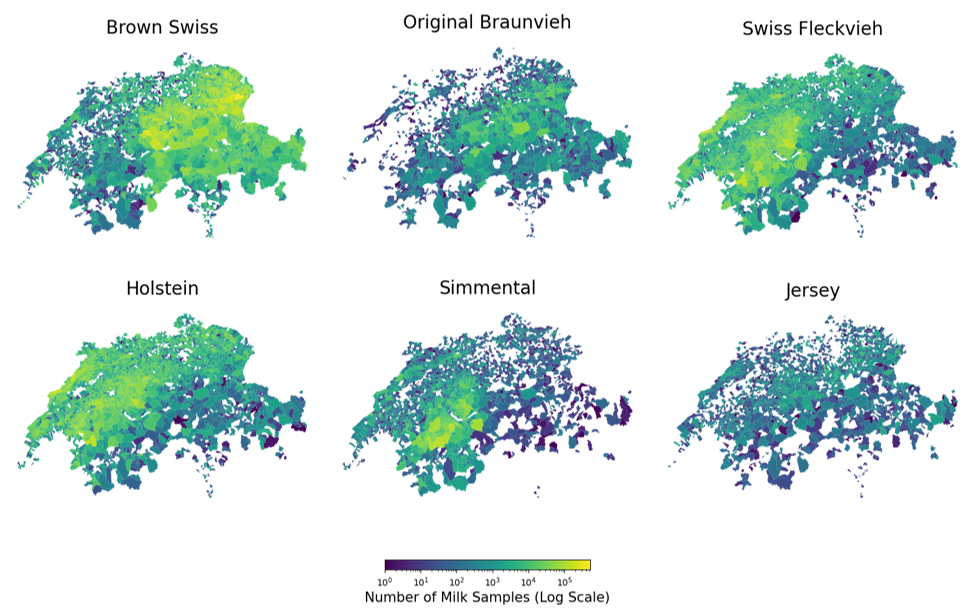
\includegraphics[width=\textwidth]{thesis/figures/dataset/sample_distribution.png}
    \caption{Sample distribution for each dairy cow breed.}
    \label{fig:dataset_sample_distribution}
\end{figure}

\subsection{Geospatial Data}\label{sec:topological_data}
The milk data described in Section~\ref{sec:agronomic_data} is provided with anonymized farm metadata with associated ZIP codes. In Switzerland, each ZIP code can be mapped to a locality. A locality is a geographically defined area designated by an unambiguous place name and unique ZIP code. The ZIP belongs to one or more political municipalities. The latter have a unique BFS\footnote{Bundesamt für Statisik - Federal Statistics Office} number assigned by the Swiss Federal Statistics Office. Since the locality distribution is more fine-granular than the political municipalities, we map each farm to the closest geographical locality center. We count a total of $3194$ localities. The geospatial data and altitude raster grids are retrieved from \cite{swisstopo_2024, swisstopo_2024_dhm25}. By matching the locality data with the milk samples ZIP codes, we delineate the geospatial distributions of samples per breed, as illustrated in Figure~\ref{fig:dataset_sample_distribution}. The Simmental and Swiss Fleckvieh populations are predominantly located in the Bernese Alps\footnote{We can also refer them as the "typical" mountain cow breeds}, whereas the Holstein breed is primarily found in Western Switzerland. In contrast, the Brown Swiss and Original Braunvieh breeds are more prevalent in eastern Switzerland. The Jersey breed, however, demonstrates a more scattered geographical distribution.



\subsection{Hydroclimatic Data}\label{sec:meteo_data}
Meteorological variables such as daily mean, minimum and maximum temperatures in [°C], precipitation [mm] and relative sunshine duration [\%] are available as a gridded dataset from \cite{ethz_2024_meteoswiss} with a 1[km]x1[km] resolution. We allocate each ZIP code locality center to the nearest point within the gridded dataset. The relative humidity is not available in gridded form. Nonetheless, the THI metric requires the relative humidity measure. \cite{meteoschweiz_2024_idaweb} offers daily mean, minimum and maximum relative humidity for some weather stations. We follow \cite{bucheli_temperature_2022} and map available height corrected stations to the closest height corrected locality centers with the following distance function: 
\begin{equation}\label{eq:station_distance_function}
    d_{s,c} = \sqrt{(\text{lat}_s - \text{lat}_c)^2 + (\text{long}_s - \text{lat}_c)^2 + \left(\psi \cdot (\text{alt}_s - \text{elevation}_c)\right)^2}.
\end{equation}
The height correction is integrated in $d_{s,c}$ as a factor $\psi=100$. This correction is applied because relative humidity is more likely to vary with elevation changes than with horizontal movements. The temperature varies with altitude and changes the saturation capacity.

\begin{figure}[htbp]
    \centering
    \begin{subfigure}[b]{0.45\textwidth}
        \centering
        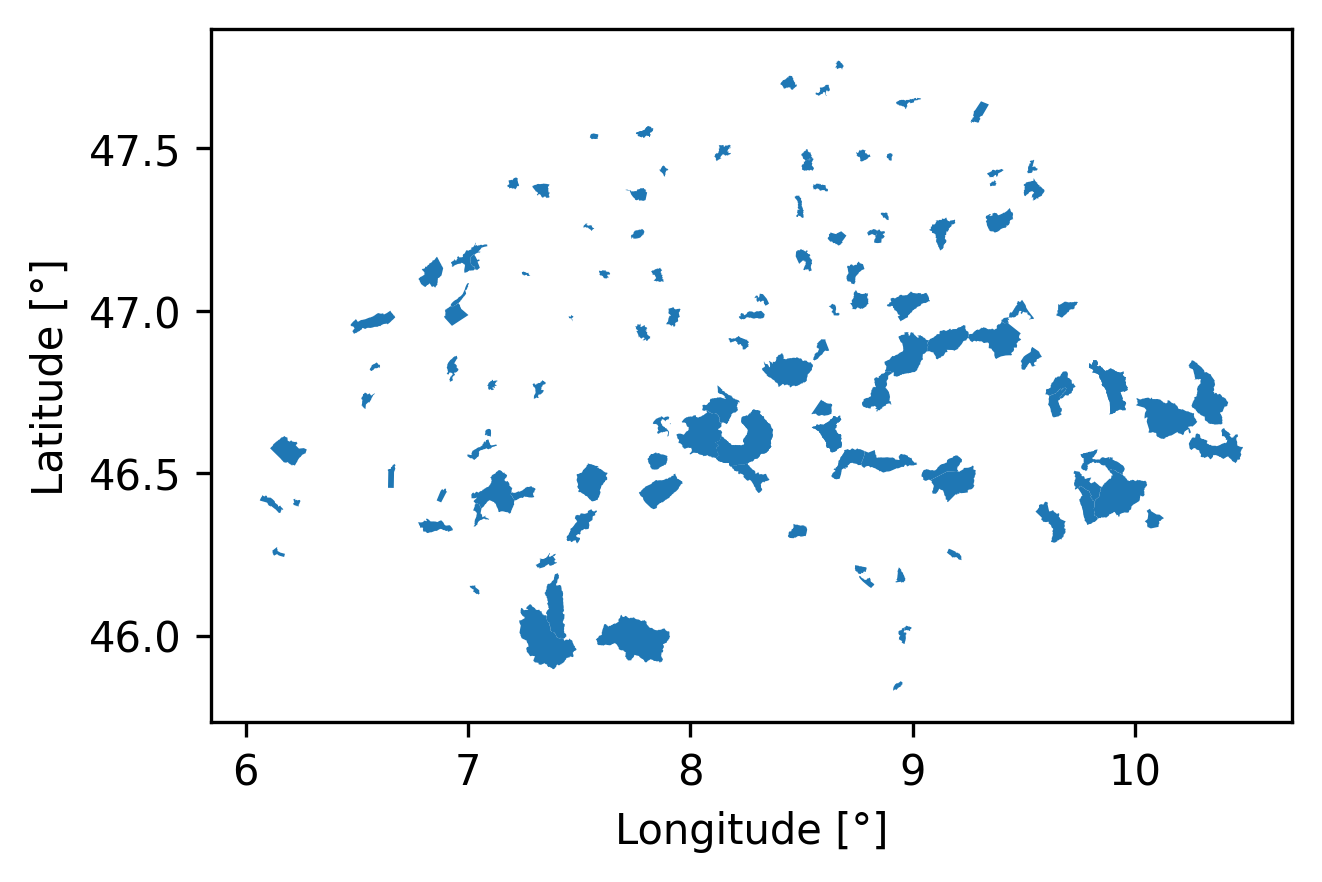
\includegraphics[width=\textwidth]{thesis/figures/weather_stations_1982.png}
        \caption{1982 - 159 Stations}
        \label{fig:weather_stations_1982}
    \end{subfigure}
    \hfill
    \begin{subfigure}[b]{0.45\textwidth}
        \centering
        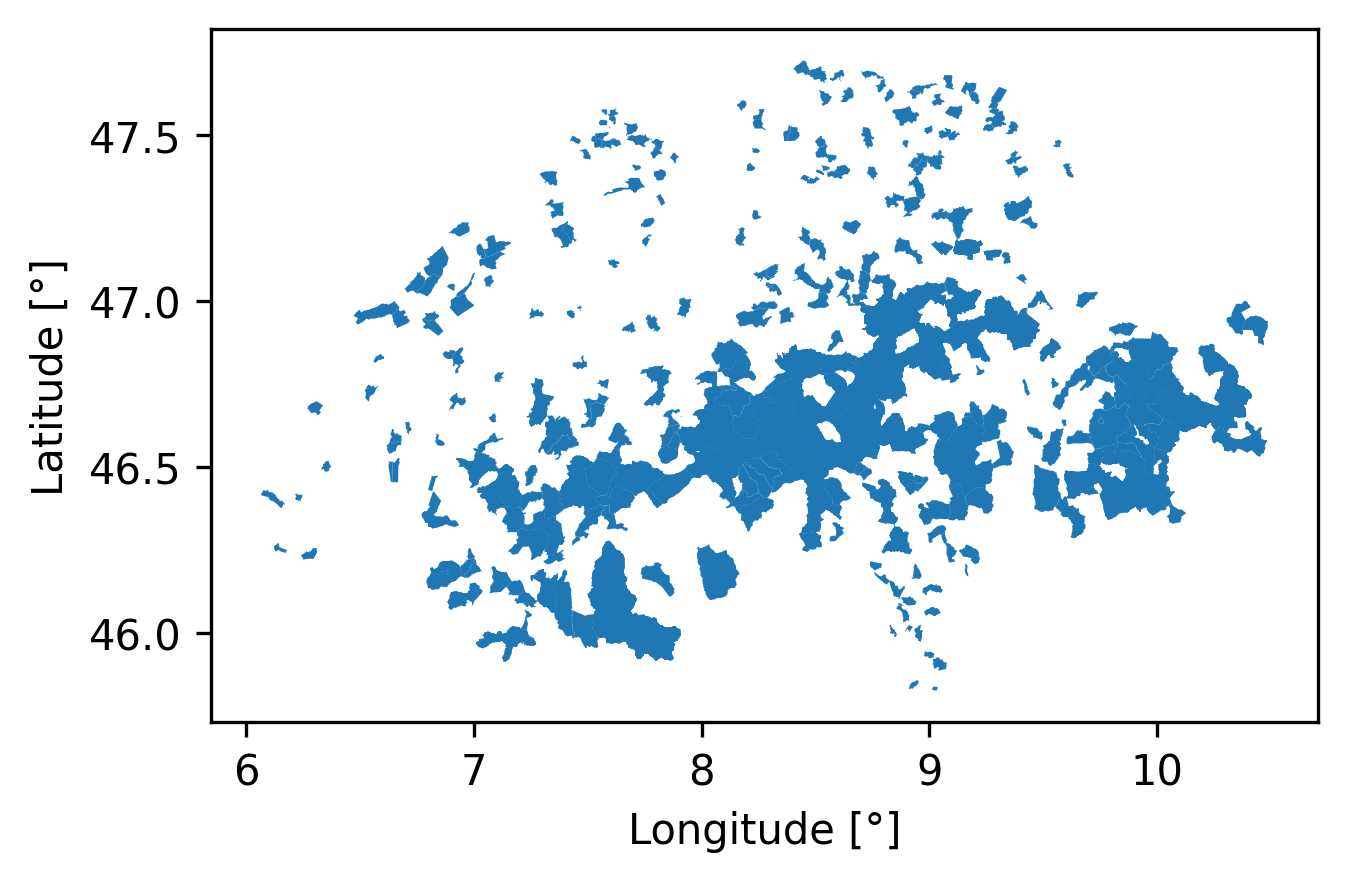
\includegraphics[width=\textwidth]{thesis/figures/weather_stations_2023.png}
        \caption{2023 - 540 Stations}
        \label{fig:weather_stations_2023}
    \end{subfigure}
    \caption{Geographical weather station distribution with available relative humidity data.}
    \label{fig:weather_stations}
\end{figure}

We retrieve all daily mean, maximum and minimum relative humidity data available from the MeteoSuisse portal from 1982 until the end of 2023. The following requirements for a station to be considered: First, the station must not have more than 500 missing samples during its lifetime. We treat a station as long as it exists as a fixed measurement point and do not control for technical changes such as hardware upgrades, which increases risk of instrumentation bias. Under these constraints, $159$ stations are available in 1982 and $540$ by the end of 2023. Figure~\ref{fig:weather_stations} shows the weather station distribution in these two years. The station concentration is increasing more in the alpine regions than in the Swiss plateau. During our study period from 1982-2024, all major regions in Switzerland are equipped with weather stations, and they increase in density over time.


\section{Models}\label{sec:models}
Informed by modeling elements derived from prior research, background information regarding dairy farming in Switzerland, biological aspects, and the organization of our data, we establish an empirical strategy. Then, we derive two model classes: single-breed models which are estimated with data for each breed-separately, and multi-breed models which are estimated with data from all breeds together. Single-breed models have lower complexity and are easier to estimate. However, this comes with statistical challenges for model comparison. A multi-breed model that explicitly models the breed aspects introduces more complexity and might be harder to estimate. However, in certain circumstances, this is more appropriate for valid statistical comparisons between breeds.

\subsection{Empirical Strategy}\label{sec:empirical_strategy}
Our goal is to estimate the average effect of THI on cow-level dairy production performance variables while controlling for breed, animal-physiological aspects, and other environmental effects such as farm management practices, regulatory changes, and breeding progress. Hence, we need an additive statistical approach to separate the THI effect from these other factors. This requirement leads us to a model with the following structure:

\begin{equation}\label{eq:empirical_strategy}
    \textit{Variable of Interest} = \textit{Weather} + \textit{Controls} + \textit{Unobserved Heterogeneity} + \textit{Error}.
\end{equation}

The \textit{variables of interest} are the daily milk yield and daily ECM yield. To estimate the average effect of weather, we need to model the THI as a component. We know from prior research that the effect of THI on milk and milk component performance is non-linear. In our models, we will use the three-day mean THI. This is the average THI value from the milk sample date $t$, $t-1$ and $t-2$: 

\begin{equation}
    \textit{3 Day Mean THI} = \frac{THI_t + THI_{t-1} + THI_{t-2}}{3},
\end{equation}
where $t$ is the reported milk sample date and 
\begin{equation}
    \text{THI}_t = (1.8 \times \text{T}_t) + 32 - \left[ (0.55 - 0.0055 \times \text{RH}_t) \times (1.8 \times \text{T}_t - 26) \right].
\end{equation}
 $T_t$ and $RH_t$ are the mean temperature and mean relative humidity of day $t$.

We opt for the three-day THI mean based on several considerations: Firstly, when a farm is sampled, cows are sampled in the morning and in the evening. These samples may either be collected on the same calendar day or across two consecutive days when the samples are taken in the evening and the morning of the following day. In the latter case, the sample date is recorded as the morning of the subsequent day; this is irrespective of the first sample being taken the day prior. The specific sequence of sampling for each set is not discernible within the dataset. Although such details are inconsequential for practical breeding operations, they become critical when aligning milk sample data with meteorological information. Consequently, it is imperative to account for weather conditions on the sampling day as well as one day prior. Secondly, we incorporate an additional preceding day to address the lagged effect of the THI on dairy cows. Currently, there is no standardized consensus on the number of lag days to be considered. However, we have aligned our methodology with the approach delineated in \cite{bryant_quantifying_2007}.

The model needs to \textit{control} for the non-linear lactation curve of the cow. Right after calving,  the milk performance increases until it reaches a peak point before it drops again until the next dry period starts. A viable proxy for this purpose is days in milk (DIM). Moreover, dairy performance also depends on the the parity - we make a binary distinction between primi- and multiparous cows. Primiparous cows have not developed their full biological potential and have a lower milk performance than multiparous cows. Moreover, we also need to control for the within-year seasonality, geospatial differences, and long-term effects such as breeding progress or regulatory changes. These aspects are motivated by the analysis of effects observed in Figure~\ref{fig:dataset_structure_time_seasonality}.

The specific characteristics of the farm location, including the barn infrastructure, the topographical features and the management strategies, cannot be explicitly measured. We assume farmers constantly adapt and change their best practices. Similarly, the fundamental performance attributed to the genetic and phenotypic attributes of individual cows cannot be directly observed. It is imperative to account for this latent heterogeneity.

\subsection{Single Breed Model}\label{sec:single_breed_model}
We first introduce a single breed model before expanding it in the next section.
Let $y_{ijkt}$ be a dairy performance variable of a sample of animal~$i$, at the farm location~$j$, at farm $k$ and at the sampling date~$t$. Equation~\ref{eq:single_breed_model_extended} defines an additive mixed model to estimate the average effect of THI on milk performance variables. The coefficient $\beta_0$ is the intercept which represents the mean performance of the given breed data, excluding all other factors included in the model. $\mathbb{I}(\text{Primiparous}_i)$ is the indicator variable whether the current cow $i$ is primi- or multiparous. $\textit{THI}_{kt}$ is the three-day mean THI at the farm location $k$ at the sampling date $t$. THI is modelled as a separate non-linear function $f_{1,1}$ and $f_{1,2}$ for primi-and multiparous cows. $\textit{DIM}_{it}$ is the days milk of the cow $i$ sampled on day $t$. Following the same analogy as for THI, DIM is also modelled separately as a non-linear function $f_{2,1}$ and $f_{2,2}$ for primi- and multiparous cows. $\beta_1$ is the fixed effect coefficient for being primiparous compared to multiparous. $\mathbb{I}(\text{Year}_t = m)$ is a variable indicating whether the sampling date $t$ falls in the year $m$, where $\mathcal{M}$ is the set of years covered by the samples included. $\beta_{2,m}$ is the effect of year $m$ compared to the reference year. $\iota_{kt}$ is the random intercept for $ZIP$ of farm $k$ and month of the sample date $t$. This random effect models the annual seasonality accounting for geospatial differences; due to the topological heterogeneity of Switzerland, timing and farming practices might vary. For example, in high-altitude regions the grazing season might start later than in the Swiss Plateau. Another aspect which is covered by this random intercept are spatial spillovers. Neighbouring farmers might apply similar practices simply due to geospatial constraints but also due to networking effects \citep{young1959neighborhood}. The factor levels for this random intercept are created with a ZIP code - month interaction term. The ZIP code is a natural choice originating from our farm-ZIP code matching introduced in Section~\ref{sec:data} and the monthly granularity is justified by the monthly sampling frequency by the breeding associations\footnote{Both of these hyperparameters are somewhat arbitrary and could be optimized in a model selection process.}. $\phi_{k}$ is the random intercept for the location of farm $k$. First, since different farms have unique characteristics such as soil, land or barn we capture the variability between farms. Moreover, Figure~\ref{fig:dataset_structure_sparsity_dynamics} shows us the hierarchical structure of the data. Grouping within entities such as farms needs to be taken into account in the model. With our data we cover very long periods of time. Farmers constantly adopt and change their practices over time. Some of the long-term national average aspects are captured by the $\textit{Year}$ fixed effect. The constant individual adaptation by each farmer is not explicitly modelled. Consequently, the effects \( f(THI) \) and \( f(DIM) \) are, at least in part, implicitly reflective of adaptive changes. Additionally, each individual cow $i$ is incorporated as a random intercept $\alpha$ to account for repeated sampling per cow and distinctive animal characteristics. The residual error term is denoted by $\epsilon_{ijkt}$.

\begin{defi}Single Breed Model - Extended Notation
\begin{equation}\label{eq:single_breed_model_extended}
    \begin{aligned}
        y_{ijkt} = & \ \beta_0 \\
        & + f_{1,1}(\text{THI}_{kt}) \cdot \mathbb{I}(\text{Primiparous}_i) \\
        & + f_{1,2}(\text{THI}_{kt}) \cdot (1 - \mathbb{I}(\text{Primiparous}_i)) \\
        & + f_{2,1}(\text{DIM}_{it}) \cdot \mathbb{I}(\text{Primiparous}_i) \\
        & + f_{2,2}(\text{DIM}_{it}) \cdot (1 - \mathbb{I}(\text{Primiparous}_i)) \\
        & + \beta_1 \cdot \mathbb{I}(\text{Primiparous}_i) \\
        & + \sum_{m \ in \mathcal{M}} \beta_{2m} \cdot \mathbb{I}(\text{Year}_t = m) \\
        & + \iota_{kt} \\
        & + \phi_k \\
        & + \alpha_i \\ 
        & + \epsilon_{ijkt} 
    \end{aligned}
\end{equation}
\end{defi}

In Equation~\ref{eq:single_breed_model} we provide a simplified notation for the model introduced in Equation~\ref{eq:single_breed_model_extended} solely focusing on the covariates and not their coefficients.

\begin{defi} Single Breed Model - Simplified Notation
\begin{equation}\label{eq:single_breed_model}
y = \mu + f(\text{THI}) \cdot \text{P} + f(\text{DIM}) \cdot \text{P} + \text{P} + \text{Y} + \iota + \phi + \alpha + \epsilon
\end{equation}
\end{defi}
The variable $y$ denotes the dependent dairy performance variable. The parameter $\mu$ serves as the overall intercept of the model. The function $f(\text{THI})$ is a non-linear function relating to the THI. Likewise, $f(\text{DIM})$ is a non-linear function that models the lactation curve. The variable $\text{P}$ signifies parity, representing a binary distinction between primiparous and multiparous cows. The term $\text{Y}$ symbolizes the year as a categorical variable, capturing potential year-to-year variations. The random intercept $\iota$ accounts for variation linked to the zip code by month, reflecting geographic and seasonality. The random intercept $\phi$ pertains to the farm location, managing variability across different farms and sampling sites. The random intercept $\alpha$ addresses the variability among individual cows. Lastly, $\epsilon$ denotes the residual error term of the model.

\subsection{Mutli-Breed Model}\label{sec:multi_breed_model}
Our hypothesis posits varying effects of THI on dairy performance across different breeds. Consequently, our aim is to determine whether there are statistically significant heterogeneous treatment effects. The treatment under consideration is the exposure of cows to weather (THI), while the heterogeneity arises from the various dairy cow breeds. Dividing the data based on breed and estimating separate models for each breed is appealing for reducing modeling complexity; however, challenges may arise if not all covariates are interacted with breed in a multi-breed model, since statistical significance is contingent upon all covariates \citep{le_interaction_term_2020}. With biological reasoning, it is justifiable to consider separate intercepts as well as interaction terms involving f(THI), f(DIM), parity, and year. The interaction of random effects for seasonality and location by breed requires further investigation. The central question pertains to whether we should assume a common biological response across breeds with respect to location and farm. Given that each cow is associated with a single breed, it should not matter whether the random intercept for cow $\alpha_i$ is interacted by breed or not. An example multi-breed models following the arguments above is

\begin{defi}
\begin{equation}\label{eq:multi_breed_model_extended}
    \begin{aligned}
        y_{ijkt} = & \ \sum_{b \in \mathcal{B}} \beta_{0,b} \cdot \mathbb{I}(B_i = b) \\
        & + \sum_{b \in \mathcal{B}} \left[ f_{1,1,b}(\text{THI}_{kt}) \cdot \mathbb{I}(\text{Primiparous}_i) \cdot \mathbb{I}(B_i = b) \right] \\
        & + \sum_{b \in \mathcal{B}} \left[ f_{1,2,b}(\text{THI}_{kt}) \cdot (1 - \mathbb{I}(\text{Primiparous}_i)) \cdot \mathbb{I}(B_i = b) \right] \\
        & + \sum_{b \in \mathcal{B}} \left[ f_{2,1,b}(\text{DIM}_{it}) \cdot \mathbb{I}(\text{Primiparous}_i) \cdot \mathbb{I}(B_i = b) \right] \\
        & + \sum_{b \in \mathcal{B}} \left[ f_{2,2,b}(\text{DIM}_{it}) \cdot (1 - \mathbb{I}(\text{Primiparous}_i)) \cdot \mathbb{I}(B_i = b) \right] \\
        & + \sum_{b \in \mathcal{B}} \left[ \beta_{1,b} \cdot \mathbb{I}(\text{Primiparous}_i) \cdot \mathbb{I}(B_i = b) \right] \\
        & + \sum_{m \in \mathcal{M}} \beta_{2m} \cdot \mathbb{I}(\text{Year}_t = m) \\
        & + \iota_{kt} \\
        & + \phi_k \\
        & + \alpha_i \\
        & + \epsilon_{ijkt},
    \end{aligned}
\end{equation}
\end{defi}

where $\mathcal{B}$ is the set of available breeds and $B_i$ a binary indicator for breed.

\subsection{Model Estimation Strategy}\label{sec:estimation_strategy}
Given the presence of repeated unbalanced measurements for cows and farms as illustrated in Table~\ref{table:dataset_statistics} and Figure~\ref{fig:dataset_structure_sparsity_dynamics}, the application of mixed models with maximum likelihood estimation is deemed appropriate for our model estimation \cite[page 61 and 74]{wood_generalized_2017}. Various methodologies exist to model the non-linear components $f$, such as binning, piecewise regression (broken stick), or splines. The contemporary approach for estimating non-linearities is through smooth terms, which can be implemented within a Generalized Additive Model framework \citep[Chapter 5 and 6]{wood_generalized_2017}. Smooth terms, being splines with penalized coefficients, facilitate a more accurate representation of the data. Consequently, we characterize our nonlinear functions $f$ as smooth terms. The components of our models are a combination of smooth terms, fixed effects, and random effects, thereby constituting Generalized Additive Mixed Models \citep[page 288]{wood_generalized_2017}. To address our research question with an estimated model, we numerically derive the turning points in the smooth terms $f$. We use \textit{mgcv} \citep{mgcv1, mgcv2, mgcv4, wood_generalized_2017, wood_gamm4_2020} for estimation and \textit{gratia} \citep{gratia} for the turning point search. This purely data-driven approach for inflection point determination is a considerable improvement compared to previous works which make preliminary assumptions about the non-linearities. Implementation details and library modifications required for our data are discussed in the following sections.


\section{From Linear Mixed Models to Generalized Additive Mixed Models}\label{sec:mixed_to_gams}
To link our model definitions in Section~\ref{sec:models} with the GAMM framework, we provide the basics around mixed models, GAMs and GAMMs and explain how they are linked. Understanding the relationship between these three frameworks is vital for a successful and computationally efficient estimation of Equation~\ref{eq:single_breed_model_extended} and Equation~\ref{eq:multi_breed_model_extended}.

\subsection{Generalized Linear Mixed Models}\label{sec:glmm}
We use the definitions from \citet{wood_generalized_2017} and \citet{bates_fitting_2015} to introduce mixed models. Let $\bm{y} \in \mathbb{R}^n$ be the response data of $n$ samples from a random variable $\mathcal{Y}$ belonging to the exponential family. Let $g(\mu_i)=\mathbf{X}_i \bm{\beta}$, where $\mu_i \equiv \mathbb{E}(Y_i)$, $g$ is the link function, $\mathbf{X}_i$ is the $i$-th row of the model matrix $\mathbf{X} \in \mathbb{R}^{n \times p}$ and $\bm{\beta} \in \mathbb{R}^p$ the vector of the  $p$ fixed effect parameters. The response variable samples $y_i$ are assumed to be independent and have a distribution that belongs to the exponential family. Let $\mathbf{Z}_i$ be the $i$-th row of the random effect model matrix $\mathbf{Z} \in \mathbb{R}^{n \times q}$ , and let $\bm{b} \in \mathbb{R}^{q}$ be the q-dimensional random vector from a random variable $\mathcal{B}\sim \mathcal N(\bm{0},\bm{\psi_{\theta}})$ containing random effects with zero expected value and covariance matrix $\bm{\psi_{\theta}} \in \mathbb{R}^{q \times q}$ with unknown parameters~$\bm{\theta}$. Let $\mathbf{\Lambda_{\theta}} \in \mathbb{R}^{n \times n}$ be the residual covariance matrix to model the residual autocorrelation. We assume that the residuals are distributed independently and identically. Hence, $\bm{\Lambda{\theta}} = \mathbf{I}\sigma^2$. This simplification comes with computational advantages, but also with modelling drawbacks regarding spatial autocorrelation in our data.
\\
\\
For the Gaussian case, a Linear Mixed Model (LMM) is defined as
\begin{defi}Linear Mixed Model
    \begin{equation}\label{eq:lmm}
    \mathbf{y} = \mathbf{X}\bm{\beta} + \mathbf{Z}\bm{b} + \bm{\epsilon}, \quad \bm{b}\sim N(\bm{0}, \bm{\psi_{\theta}}), \quad \bm{\epsilon} \sim \mathcal(\bm{0}, \bm{\Lambda_{\theta}}) = N(\bm{0},\mathbf{I}\sigma^2), 
    \end{equation}
\end{defi}
where $y\sim N(\mathbf{X}\bm{\beta}, \mathbf{Z}\bm{\psi_\theta}\mathbf{Z}^T + \mathbf{I}\sigma^2)$ and $(Y | \mathcal{B} = \bm{b}) \sim \mathcal{N}(\mathbf{X}\bm{\beta} + \mathbf{Z}\bm{b}, \sigma^2 \bm{I})$.
\\
\\
The extension of an LMM to non-normal data is given as the Generalized Linear Mixed Model (GLMM) with
\begin{defi}Generalized Linear Mixed Model
    \begin{equation}\label{eq:glmm}
        g({\mu}) =  \mathbf{X}\bm{\beta} + \mathbf{Z}\bm{b}, \quad \bm{b}\sim \mathcal{N}(\bm{0}, \bm{\psi_{\theta}}),
    \end{equation}
\end{defi}
where $(\mathcal{Y} | \mathcal{B} = \bm{b}) \sim \mathcal{D}(g^{-1}(\mathbf{X}\bm{b} + \mathbf{Z}\bm{b}), \phi)$ and $\mathcal{B} \sim \mathcal{N}(\bm{0}, \bm{\psi_{\theta}})$. $\mathcal{D}$ is the distribution of the exponential family, and $\phi$ is a common scale parameter. The error term in Equation~\ref{eq:lmm} comes from the normal distribution of the response variable $\mathcal{Y}$. The remaining variability is related to the assumed distribution~$\mathcal{D}$. Therefore, no explicit error term $\bm{\epsilon}$ is available in the generalized case.

\subsection{Generalized Additive Models}
Generalized Additive models are a flexible generalization of linear models accommodating non-linear relationships between predictors and outcome variables through smooth terms. The smooth terms enable us to capture these non-linear relationships without further specifying the non-linear structure in advance. The additive principle between the individual effects remains as in regular linear regression models. In addition, GAMs incorporate different link functions to support different types of response variables with various distributions from the exponential family. 
\\
\\
In contrast to the fixed effect model matrix $\mathbf{X}$ in Sec.~\ref{sec:glmm} we introduce a model matrix $\mathbf{X^*}$ for the strictly parametric part, where $\mathbf{X^*_i}$ is the $i$-th row of this design matrix. The corresponding parametric vector is defined as $\bm{\beta^*}$. Let $f_j$ be the smooth function of the covariates $\bm{x}_j$, where a smooth function $f_j$ may be a function of one or more covariates \citep{wood_generalized_2017, wood_stable_2004}. The matrix $\mathbf{x_j} \in \mathbb{R}^{n \times |f_j|}$ comprises samples for the covariates assigned to the smooth $f_j$. Therefore, the smooth components may be uni- or multivariate. This leads to the definition of a GAM as the sum of smooth functions given by 
\begin{defi}Generalized Additive Model
    \begin{equation}\label{eq:gam}
    g(\mu_i) = \mathbf{X_i^*}\bm{\beta^*} + f_1(x_{1i}) + f(x_{2i}) + \dots,
    \end{equation}
\end{defi}

where some or all covariates are represented with a smooth term. The smooth terms can be understood as a basis expansions for the associates covariates, where the smoothness is controlled by penalty terms. A common way to fit GAMs and choose the appropriate smoothness are likelihood maximization methods such as the Restricted Maximum Likelihood Method (REML) \citep{corbeil_restricted_1976}. 

\subsection{Generalized Additive Mixed Models}
There is a mathematical equivalence between smooth terms and random effects \citep[p. 239]{wood_generalized_2017}. Simple random effect structures $\mathbf{Z}$ with random intercepts and random slopes can be defined as smooth terms $f_j(z_j)$ and are fitted with \textit{gam} by default or \textit{bam} for large datasets \citep{wood_generalized_2015, wood_mgcv_2023}. Equation~\ref{eq:gamm_smooth} illustrates this equivalence. Hence, a GAM with random effect structures, a generalized additive mixed model (GAMM), can be represented and fitted in the form of a GAM defined in Equation~\ref{eq:gam}. Further implementation details for random effects as smooth terms are available in \cite{mgcv_smooth_construct}. These are not further discussed in the scope of this work.

\begin{defi}Generalized Additive Mixed Model
\begin{equation}\label{eq:gamm_smooth}
    g(\mu_i) = \mathbf{X_i^*}\bm{\beta^*} + f_1(x_{1i}) + f(x_{2i}) + \dots + \mathbf{Z_i}\bm{b} \equiv \mathbf{X_i^*}\bm{\beta^*} + f_1(x_{1i}) + f(x_{2i}) + \dots + f_1(z_{1i}) + f(z_{2i}) + \dots,
\end{equation}
\end{defi}

Random effect structures often come with sparsity. The aforementioned default implementations do not take advantage of this sparse effect structure. For a modest number random effects these methods are still computationally appealing. However, \textit{mgcv} is not optimized for a growing number of group factor levels for random effect structures. \citet{brooks_glmmtmb_2017} highlight the exponentially growing estimation time with a growing number of random effect levels using the default routines in the aforementioned library. For a large number of random effect factor levels, the duality principle between GAMs and GLMMs permits the reformulation of a GAMM as a GLMM. Let $\bm{f}_j$ be the vector of a smooth from a sample $i$, $f_{ij}=f(x_{ij})$. Each smooth term has one or more basis functions. The collection of basis functions within a smooth can be interpreted as a vector.

In the mixed model form $\bm{f}_j=\mathbf{X'}_j\bm{\beta'}_j + \mathbf{Z'}_j\bm{b'}_j$, where $\bm{b'}_j \sim \mathcal{N}(\bm{0}, \bm{I}\sigma^2_{b_{j}})$. The columns of $\mathbf{X'}_j$ are a null space basis of the smoothing penalty. Equivalently, the columns of $\mathbf{Z'}_j$ are the range basis. More specifically, each smooth term corresponds to a fixed effect part $\mathbf{X'}_j$ and a random effect part $\mathbf{Z'}_{j}$. Let $\mathbf{X'_\Sigma}$ be the combined effect concatenated from the individual smooth fixed effects $\bm{X'}_j$ and $\mathbf{Z'_\Sigma}$ the combined smooth term random matrix concatenated from the individual $\mathbf{Z}'_{j}$. Hence, generalizing to an arbitrary number of smooths, a GAMM as a GLMM is defined as

\begin{defi}Generalized Additive Model as Generalized Linear Mixed Model
\begin{equation}\label{eq:gamm_glmm}
    g(\mu_i) = \mathbf{X_i^*}\bm{\beta^*} + f_1(x_{1i}) + f(x_{2i}) + \dots + \mathbf{Z_i}\bm{b} \equiv \mathbf{X_i^*}\bm{\beta^*} + \mathbf{X'_{i \Sigma}}\bm{\beta'_{\Sigma}} +\mathbf{Z'_{i \Sigma}}\bm{b'_{\Sigma}} + \mathbf{Z_i}\bm{b}.
\end{equation}
\end{defi}

The individual fixed effect terms $\mathbf{X_i^*}\bm{\beta^*} + \mathbf{X'_{i \Sigma}}\bm{\beta'_{\Sigma}}$ and the individual random effect terms $\mathbf{Z'_{i \Sigma}}\bm{b'_{\Sigma}} + \mathbf{Z_i}\bm{b}$ in Equation~\ref{eq:gamm_glmm} can be concatenated into one fixed effect and one random effect structure as in Equation~\ref{eq:glmm}. This concludes our definition of GAMMs as mixed models. In R, \textit{gamm}\citep{wood_mgcv_2023} and \textit{gamm4} \citep{wood_gamm4_2020} are the available routines for estimating GAMs with mixed models engines. \textit{gamm} uses \textit{nlme} \citep{pinheiro2017package} and \textit{gamm4} uses \textit{lme4} \citep{bates_fitting_2015} as the underlying engine.

\section{Estimating Generalized Additive Mixed Models}\label{sec:estimating_gams}
In Section~\ref{sec:agronomic_data} we discuss the sparsity of our data. Estimating our model with cows and farms as random intercepts for representative subsamples covering a broad range of weather data points results in tens of thousands of random effect factor levels. Therefore, the default methods \textit{gam} and \textit{bam} are computationally not appropriate for estimations with reasonable model fitting times and memory consumption. This is because the sparse structure of random effects is not leveraged when using the random-effect-as-smooth approach given in Equation~\ref{eq:gamm_smooth}. In the following Section~\ref{sec:gam_bam}, we briefly discuss some subsampling strategies with which we experiment to potentially circumvent these limitations, before discussing other off-the-shelf approaches. Since these are not successful, we discuss the development of an appropriate alternative method in detail in the last subsection. All experiments in this study are performed on a 32 core machine with 512 GB of RAM.

\subsection{gam and bam}\label{sec:gam_bam}
We explore various variants of the multi-breed model as delineated in Equation~\ref{eq:gam_bam} by employing different subsampling methodologies. 
\begin{defi}  Multi-Breed Model for \textit{bam} and \textit{gam} Experiments
    \begin{equation}\label{eq:gam_bam}
    \text{milk} = \mu + B + f(\text{THI})\times B + \text{DIM}\times B + \text{P} + \text{Y} + \phi + \alpha + \epsilon.
\end{equation}
\end{defi}
Model~\ref{eq:gam_bam} represents a simplification of the multi-breed model proposed in Equation~\ref{eq:multi_breed_model_extended}. The term ‘different variants’ pertains to experiments involving diverse breed interaction terms, varying smooth terms, and the interaction of farm intercepts with ZIP codes $\phi$. We refrain from providing an exhaustive list of options due to the recurrent challenges we encounter: Firstly, with a limited number of samples, the smooth terms, upon visual inspection, appear biologically nonsensical. Secondly, increasing the sample size leads to a substantial rise in model estimation time and the computational load of the \textit{summary} function. Thirdly, memory constraints become apparent when the sample size is excessively large. Fourthly, while simplifying the model by removing random effect terms like the animal intercepts permits the estimation of models with larger sample sizes, the resultant smooth terms remain biologically unintelligible. Fifthly, we implement several subsampling techniques to curtail the number of farms and animals considered, while retaining geospatial diversity and ensuring adequate breed representation.

In all scenarios, the models either fail to converge, encounter memory issues, or yield meaningless outcomes. A sampling strategy suggested by the ETH Statistical Consulting Service involves selecting a single sample per farm and omitting the modeling of animal random intercepts. Theoretically, given the extensive number of farms in our dataset (Table~\ref{table:dataset_statistics}), the quantity of data points should suffice for modeling the smooth terms. Additionally, this method could potentially alleviate violations of \textit{iid} error term assumptions and spatial autocorrelation challenges. Nevertheless, even with this approach, obtaining biologically meaningful smooths remains elusive. While adhering to the research objective of estimating smooth terms to ascertain the non-linear impact of THI, we resolve to investigate alternative methodologies such as \textit{gamm4}.


\subsection{gamm4}
\textit{gamm4} estimates GAMs as mixed models with \textit{lme4} as the underlying engine which has sparse matrix support and is known to be efficient. The \textit{gamm4} routine performs three steps: First, in the pre-processing phase, a GAMM model is converted into a GLMM. Second, in the fitting-phase, the parameter estimation is executed with the \textit{lme4} engine. Third, the estimated parameters are re-transformed into a GAM specification, and the confidence intervals for the smooth terms are estimated. This step is crucial for practical purposes and allows the fitted model to be treated as a regular GAM for downstream model analysis, diagnostics, as well as inference.

We run several experiments to assess the performance of \textit{gamm4} for a single breed model with the Jersey data: 
\begin{defi} Simple Single Breed Model for \textit{gamm4} Performance Assessment
    \begin{equation}\label{eq:gamm4_model}
    \text{milk} = \beta_0 + f(\text{THI}) + \beta_1 \cdot \text{DIM} + \beta_2 \cdot \text{P} + \text{Y} + \phi + \alpha + \epsilon.
\end{equation}
\end{defi}


Table~\ref{table:gamm4_performance} illustrates that the estimation times rise as the levels of random effect factors increase. Unlike the subsampling experiments and modeling trade-offs using \textit{gam} and \textit{bam} outlined earlier, \textit{gamm4} enables us to achieve biologically meaningful outcomes, evidenced by the visual credibility of the smooth terms for THI, especially for the last experiment listed. This observation provides us some indication about the number of samples required to build accurate multi-breed models.

The model used for this experiment does not correspond to a mature single-breed model and is designed primarily for performance assessment purposes. For example, modelling the DIM as a fixed effect instead as a smooth term, or interacting farms with the month of the year, are limitations. The main goal of this comparison is to emphasize the performance implications of varying factor levels. This analysis reveals the computational difficulties to be encountered as the number of samples and factor levels grow, particularly with larger and more representative data subsets or multi-breed models. Simple experiments with multiple breeds over a million of samples explode in execution time or fail with memory errors during a Cholesky decomposition step.

\begin{table}[H]
\centering
\begin{tabular}{r r r r}
\textbf{\# Samples} & \textbf{\# Cows} $\alpha$ & \textbf{\# Farm $\times$ Month} $\phi$ & \textbf{Fitting Time [s]} \\
\hline
\hline
175'346 & 24'170 & 10'000 & 342 \\
259'088 & 25'433 & 15'000 & 822 \\
426'397 & 26'201 & 25'000 & 2'332 \\
660'110 & 26'641 & 39'223 & 5'447\\
\end{tabular}
\captionsetup{width=0.65\linewidth}
\caption{\textit{gamm4} execution times with a growing number of samples and random effect factor levels.}\label{table:gamm4_performance}
\end{table}

\subsection{MixedModels.jl}
An alternative mixed model library to \textit{lme4} is \textit{MixedModels.jl} implemented in Julia in contrast with previous libraries that use R. The latter is notably faster\footnote{According to ETH Statistical Consulting up to 30 times faster} than \textit{lme4} \citep{markwick_fitting_2022}. GAMs cannot be estimated with the default \textit{MixedModels.jl} interface. However, the mechanisms implemented in \textit{gamm4} could be modified to execute the model fitting step with the high-performance and memory-efficient Julia library. To assess if \textit{MixedModels.jl} is suitable and scales with our data, we perform an experiment with the following model inspired by \cite{bryant_quantifying_2007}: 



\begin{defi} Multi-Breed Model for \textit{MixedModels.jl} Performance Assessment
\begin{equation}\label{eq:lmm_julia}
\begin{aligned}
\text{milk} &= \beta_0 + \sum_{i=1}^{n_B} \beta_{1i} \cdot B_i + \sum_{k=1}^{n_Y} \beta_{2k} \cdot Y_k + \beta_3 \cdot P + \sum_{i=1}^{n_B} \beta_{4i} \cdot (B_i \times \text{THI}) + \sum_{i=1}^{n_B} \beta_{5i} \cdot (B_i \times \text{THI}^2) \\
&\quad + \sum_{i=1}^{n_B} \beta_{6i} \cdot (B_i \times \text{DIM})  + \alpha + \phi + \epsilon,
\end{aligned}
\end{equation}
\end{defi}

where $n_B$ is the number of breeds and $n_Y$ the number of years.

\begin{table}[H]
\centering
\begin{tabular}{r|c|r|r|r}
\textbf{\# Samples} & \textbf{Breeds} & \textbf{\# Cows} & \textbf{\# Farm $\times$ Month} & \textbf{Fitting Time [s]} \\
\hline
\hline
660'110 & JE & 26'641 & 39'223 & 580\\
7'381'552 & HO, JE, SF, SI, BS, OB & 1'833'470 & 106'642 & 15'231\\
\end{tabular}
\captionsetup{width=0.95\linewidth}
\caption{\textit{MixedModels.jl} execution times with a Jersey only model and a six-breed model. The Jersey model is fitted without the $\text{THI}^2$ term.}\label{table:mixedmodeljl_performance}
\end{table}

Table~\ref{table:mixedmodeljl_performance} shows the model estimation times for two data subsets. These results confirm the scalability assumption for \textit{MixedModels.jl} with millions of factor levels with acceptable execution times and low memory consumption\footnote{memory consumption at Gigabytes for the process - \textit{htop} observations during runtime - no systematic profiling}. With the goal to fit a multi-breed GAM, with millions of samples, we decide to modify \textit{gamm4} and replace the \textit{lme4} estimation engine with \textit{MixedModels.jl}.

\subsection{Putting it all together: \textit{gamm4} Modifications}\label{sec:gamm4_modifications}
In order to overcome challenges described in previous subsections, we study the libraries and identify opportunities for their enhancement and combination to achieve our goals.

\textit{gamm4} implements the GAMM mixed model equivalence described in Equation~\ref{eq:gamm_glmm}. During our source code analysis, with the goal to understand how to translate a mixed model prepared for \textit{lme4}  to a \textit{MixedModels.jl} format, we discover bottlenecks during the pre- and post-processing phases in \textit{gamm4}. Therefore, we develop two distinct modified library versions: A first version, \textit{gamm4b}, which fixes bottlenecks during the pre-and post-processing phases and still estimates the model parameters with \textit{lme4}. A second version, \textit{gammJ} which modifies the pre-processing to estimate the parameters with a modified version of \textit{MixedModels.jl} and also further optimizes the post-processing steps. A modified \textit{MixedModels.jl} is required to support the mixed model structures generated by Equation~\ref{eq:gamm_glmm}. To summarize, the artifacts of our effort to accommodate a larger number of factors levels in GAMMs are threefold: First, the bug-fixed and accelerated \textit{gamm4} library, which we refer to as \textit{gamm4b}. Second, the \textit{gammJ} prototype which executed the model fitting in a modified \textit{MixedModels.jl}. Third, the modified \textit{MixedModels.jl} which supports a broader set of mixed models than the default version. These three contributions must be considered as prototypes.

\subsubsection{gamm4b}\label{sec:gamm4b}
In this section, we summarize the three major modifications to \textit{gamm4} while still using \textit{lme4} as the underlying mixed model parameter estimation engine. We plan to share these modifications with the authors of \cite{wood_gamm4_2020} since these are relatively simple but powerful changes to the existing \textit{gamm4} source code, assuming a setup with R and Python is available.

\paragraph{Random Effect Matrix Substitution Process}
When a smooth term $f_j$ is converted to its fixed effect part $\mathbf{X'_j}$ and the random effect part $\mathbf{Z'_j}$, the number of columns in the random effect matrix depends on the number of basis functions of the smooth $j$. \textit{lme4}'s regular user interface does not support arbitrary random effect matrices. They are generated by R's formula interface for particular random intercept and random slope structures. Hence, the random effect matrices $\mathbf{Z}$ generated with this interface do only over a subset of models which could be fitted with the underlying engine. The latter supports a broader set of random effect matrices\footnote{Further specifications about potential constraints are out of scope for this work.}, including the $\mathbf{Z'_j}$ generated by the GAMM to GLMM model conversion. In \textit{gamm4} the following trick is applied: Consider each smooth term as a random intercept with $k$ factor levels, where $k$ is the number of basis functions for the given smooth. The \textit{lme4} model building process then allocates the corresponding columns in the $\mathbf{Z}$ matrix with a regular binary random intercept structure. Then replace the corresponding columns in the generated $\mathbf{Z}$ with the $\mathbf{Z'_j}$ from the smooth to random effect conversion. This replacement process, a sparse matrix substitution, is extremely inefficiently implemented and is a limitation of \cite{bates_matrix_2024}. The performance impact becomes noticeable when fitting models with hundreds of thousands of samples with tens of thousands of random factor levels, where this step takes up to thousands of seconds in our debugging analysis. Our first contribution to \textit{gamm4b} is a more efficient implementation of this sparse matrix substitution process. More specifically, lines 225 - 235 of the \href{https://github.com/cran/gamm4/blob/master/R/gamm4.r}{\textit{gamm4 source code}} are replaced.

\paragraph{Default Optimizer Parameter Bug Fix}
During our \textit{gamm4} dissection process, we discover a parameter error on the \textit{gamm4} source code line 237. A custom optimizer parameter passed to the \textit{gamm4} routine is not properly passed to the underlying fitting engine. This discovery is made because during the \textit{gammJ} (Section~\ref{sec:gammJ}) development we use \textit{gamm4} as a reference implementation to compare the estimated parameters with the estimates in \textit{MixedModels.jl}. Generally, we use the BOBYQA optimizer \citep{powell_bobyqa_2009} in all our experiments. Presumably, this is also the default optimizer in \textit{lme4}. However, we observe differences in the estimated parameters and debugging outputs when we do not specifically pass \textit{"bobyqa"} as the optimizer argument in \href{https://search.r-project.org/CRAN/refmans/lme4/html/lmerControl.html}{\textit{lmerControl}}.

\paragraph{Post-Processing Cholesky Decomposition}
Using our GAMM definition from Equation~\ref{eq:gamm_glmm}, let $\mathbf{Z}$ be the random effects model matrix of the non-smooth terms and let $\bm{\psi_\theta}$ be the corresponding random coefficient matrix associated with the estimated random effect parameters. The post-processing step to fully represent the fitted GLMM as a GAM includes the computation of the data covariance matrix  
\begin{equation}\label{eq:data_covariance}
    \mathbf{V} = \mathbf{Z} \, \bm{\overline{\psi}_\theta} \, \mathbf{Z}^{\top} + \mathbf{I}\sigma^2.
\end{equation}
The inverse of $\mathbf{V}$, $\mathbf{V}^{-1}$ is used for further downstream computations. $\mathbf{V} \in \mathcal{R}^{n \times n}$ is growing quadratically with the number of samples. \citep[page 289]{wood_generalized_2017} warn about the computational complexity and advise to leverage the special structure of $\mathbf{V}$. Since $\mathbf{V}$ is symmetric and positive-definite, a Cholesky decomposition can be applied. \textit{gamm4} implements a Cholesky decomposition on line 374 with functionality from the \cite{bates_matrix_2024} library. The construction of $\mathbf{V}$ and the computation of its Cholesky decomposition do not scale well with our data. We replace the Cholesky decomposition with a Python call \citep{reticulate} to the \textit{Cholmod} \citep{chen_algorithm_2008} function of \href{https://github.com/scikit-sparse/scikit-sparse}{\textit{scikit-sparse}} to overcome this limitation. In our experiments, with this modification, we can estimate GAMMs up to a sample size up to approximately 500'000 to 750'000, depending on the exact random effects structure. Larger sizes lead to memory allocation problems in R because the sparse matrix indexing in \cite{bates_matrix_2024} only supports 32-bit indexes, which is not sufficient with our size of $\mathbf{V}$. This further motivated the exploration of Julia software packages to avoid the limitations of R libraries.

\subsubsection{gammJ}\label{sec:gammJ}
With \textit{gammJ} we fit GAMMs as mixed models in a modified \textit{MixedModels.jl} and apply further optimizations to operations related to the data covariance matrix introduced in Equation~\ref{eq:data_covariance}. These modifications further accelerate the estimation process and remove the matrix 32-bit indexing issues described in Section~\ref{sec:gamm4b}. In Section~\ref{sec:julia_modifications} we describe our modifications applied to \textit{MixedModels.jl} to accommodate GAMMs as GLMMs. In Section~\ref{sec:cholesky_scalable} we specify implementations details for operations related to $\mathbf{V}$.


\subsubsection{Extended MixedModels.jl to support GAMMs as GLMMs}\label{sec:julia_modifications}
\textit{MixedModels.jl} is very similar to \textit{lme4} and is partially developed by the same authors \citep{bates_fitting_2015, MixedModelsJl}. However, the library is faster in many scenarios because the implementation leverages particular matrix structures and optimizes the corresponding operations. A key equation for estimating the mixed effect problem as given in Equation~\ref{eq:lmm} and Equation~\ref{eq:glmm}, is the Cholesky decomposition given in \citet[page 14, equation 18]{bates_fitting_2015}:

\begin{equation}\label{eq:lme4_cholesky}
\left[ \begin{array}{cc}
\Lambda_{\theta}^\top \mathbf{Z}^\top \mathbf{W} \mathbf{Z} \Lambda_{\theta} + \mathbf{I} & \Lambda_{\theta}^\top \mathbf{Z}^\top \mathbf{W} \mathbf{X} \\
\mathbf{X}^\top \mathbf{W} \mathbf{Z} \Lambda_{\theta} & \mathbf{X}^\top \mathbf{W} \mathbf{X}
\end{array} \right]
=
\left[ \begin{array}{cc}
\mathbf{L}_{\theta} & 0 \\
\mathbf{R}_{ZX}^\top & \mathbf{R}_{X}
\end{array} \right]
\left[ \begin{array}{cc}
\mathbf{L}_{\theta}^\top & \mathbf{R}_{ZX} \\
0 & \mathbf{R}_{X}
\end{array} \right]
= \mathbf{L}\mathbf{L}^{\top}.
\end{equation}

As previously defined in Equation~\ref{eq:lmm} and Equation~\ref{eq:glmm} the matrix $\mathbf{Z}$ is the random effects design matrix while $\mathbf{X}$ is the design matrix for the fixed effects. The relative covariance factor $\Lambda_{\theta}$ represents a block-diagonal matrix that consists of blocks associated with the variance components of the random effects. Each block $\Lambda_i$ corresponds to a specific random effect term and is a function of the parameter vector $\bm{\theta}$, which defines the random effects' variance structure. $\mathbf{W}$ is a diagonal weight matrix, typically $\mathbf{I}$. $\mathbf{L}_{\theta}$~is the lower triangular Cholesky factor of $\Lambda_{\theta}^\top \mathbf{Z}^\top \mathbf{W} \mathbf{Z} \Lambda_{\theta} + \mathbf{I}$ and plays a crucial role in simplifying the computation of the variance components during the estimation process. $\mathbf{R}_{ZX} = \mathbf{X}^\top \mathbf{W} \mathbf{Z} \Lambda_{\theta}$ describes the interaction between the fixed and random effects. Finally, $\mathbf{R}_{X}$ is the upper triangular Cholesky factor of the fixed-effects cross-product matrix $\mathbf{X}^\top \mathbf{W} \mathbf{X}$. All these matrices work together and enable the estimation of both fixed and random effects in the model. The curious reader is invited to consult \cite{bates_fitting_2015} for more details on the meaning of the individual matrices in Equation~\ref{eq:lme4_cholesky}.

The random effects matrix $\mathbf{Z}$ has a blocked structure if there are multiple random effects such as cows and farms in our case. Moreover, depending on the nature of the individual random effects or slopes, the entries of the individual matrix blocks can be as simple as binary for random intercepts or real numbers for slopes. In many cases, the blocks are sparse. \textit{MixedModels.jl} optimizes for many of these aspects. Let us consider a model with $q$ random effects, resulting in a random effects matrix $\mathbf{Z}=\begin{bmatrix} \mathbf{Z}_1 & \mathbf{Z}_2 & \dots & \mathbf{Z}_q \end{bmatrix}$ and the corresponding relative covariance factor $\mathbf{\Lambda}_{\theta} = \text{diag}\left( \Lambda_{\theta_1}, \Lambda_{\theta_2}, \dots, \Lambda_{\theta_q} \right)$, both with $q$ blocks. Expanding the left-hand side of Equation~\ref{eq:lme4_cholesky} leads to

\begin{equation}\label{eq:lme4_cholesky_blocked}
\left[
\begin{array}{cc}
\begin{bmatrix}
\Lambda_{\theta_1}^\top \mathbf{Z}_1^\top \mathbf{W} \mathbf{Z}_1 \Lambda_{\theta_1} + \mathbf{I}_1 & \dots & \Lambda_{\theta_1}^\top \mathbf{Z}_1^\top \mathbf{W} \mathbf{Z}_q \Lambda_{\theta_q} \\
\vdots & \ddots & \vdots \\
\Lambda_{\theta_q}^\top \mathbf{Z}_q^\top \mathbf{W} \mathbf{Z}_1 \Lambda_{\theta_1} & \dots & \Lambda_{\theta_q}^\top \mathbf{Z}_q^\top \mathbf{W} \mathbf{Z}_q \Lambda_{\theta_q} + \mathbf{I}_q
\end{bmatrix} 
&
\begin{bmatrix}
\Lambda_{\theta_1}^\top \mathbf{Z}_1^\top \mathbf{W} \mathbf{X} \\
\vdots \\
\Lambda_{\theta_q}^\top \mathbf{Z}_q^\top \mathbf{W} \mathbf{X}
\end{bmatrix}
\\
\begin{bmatrix}
\mathbf{X}^\top \mathbf{W} \mathbf{Z}_1 \Lambda_{\theta_1} & \dots & \mathbf{X}^\top \mathbf{W} \mathbf{Z}_q \Lambda_{\theta_q}
\end{bmatrix}
&
\mathbf{X}^\top \mathbf{W} \mathbf{X}
\end{array}
\right].
\end{equation}

$\mathbf{L}$ of the right-hand side of Equation~\ref{eq:lme4_cholesky} expands to 

\begin{equation}
\mathbf{L} =
\left[
\begin{array}{cc}
\begin{bmatrix}
\mathbf{L}_{\theta_1} & 0 & \dots & 0 \\
\mathbf{L}_{21} & \mathbf{L}_{\theta_2} & \dots & 0 \\
\vdots & \vdots & \ddots & 0 \\
\mathbf{L}_{q1} & \mathbf{L}_{q2} & \dots & \mathbf{L}_{\theta_q}
\end{bmatrix}
&
0 \\
\begin{bmatrix}
\mathbf{X}^\top \mathbf{W} \mathbf{Z}_1 \Lambda_{\theta_1} & \dots & \mathbf{X}^\top \mathbf{W} \mathbf{Z}_q \Lambda_{\theta_q}
\end{bmatrix}
&
\mathbf{R}_{X}
\end{array}
\right], 
\end{equation}
where the top-left block is the lower triangular Cholesky factor $\mathbf{L}_{\theta}$ of the block random effects matrix. This block matrix consists of the Cholesky factor $\mathbf{L}_{\theta_i}$ of each block $\Lambda_{\theta_i}^\top \mathbf{Z}_i^\top \mathbf{W} \mathbf{Z}_i \Lambda_{\theta_i} + \mathbf{I}_i$ and the Cholesky factor $\mathbf{L}_{ij}$ of the cross terms between different random effects blocks $\Lambda_{\theta_i}^\top \mathbf{Z}_i^\top \mathbf{W} \mathbf{Z}_j \Lambda_{\theta_j}$. The top-right block is $0$ because the lower triangular matrix has zeros above the diagonal. The bottom-left block contains the interactions between the fixed-effects design matrix and the random effects blocks, i.e., $\mathbf{R}_{ZX}^\top = \begin{bmatrix} \mathbf{X}^\top \mathbf{W} \mathbf{Z}_1 \Lambda_{\theta_1} & \dots & \mathbf{X}^\top \mathbf{W} \mathbf{Z}_q \Lambda_{\theta_q} \end{bmatrix}$. The bottom-right block $\mathbf{R}_{X}$ is the Cholesky factor of the fixed-effects design matrix cross-product $\mathbf{X}^\top \mathbf{W} \mathbf{X}$.

The different $\mathbf{Z}_q$ have different structures depending on the model definition. For example if a block $\mathbf{Z_q}$ corresponds to a random intercept, the columns of the matrix are indicator columns and the operation $\mathbf{Z}_q^{\top}\mathbf{Z}_q$ leads to a block diagonal matrix. \textit{MixedModels.jl} supports different $\mathbf{Z}_q$ blocks structures and implements optimized matrix operations between them, accounting for all possible term interactions resulting from Equation~\ref{eq:lme4_cholesky_blocked}. However, the block structure $\mathbf{Z}'_j$ resulting from a smooth term from a GAMM to GLMM conversion and the corresponding matrix multiplications are not supported in \textit{MixedModels.jl}. Our extension adds this block type, referred as \textit{FlexReMat} type in our source code, and the associated matrix operations. Some sparse matrix operations are not fully optimized in our implementation, and open opportunities for additional improvements. Moreover, at the current stage, tests have only been executed for \textit{REML} and the Gaussian family with the identity link function. 

\subsubsection{Scalable Cholesky Decomposition of Data Covariance Matrix}\label{sec:cholesky_scalable}
To overcome the computational limitations presented in Section~\ref{sec:gamm4b} of the data covariance matrix~$\mathbf{V}$ operations we implement a scalable Julia version with the latest high-performance sparse matrix library \textit{SuiteSparseGraphBlas.jl} \citep{GraphBLAS7, graphblas_1000, graphblas_julia} and \textit{CHOLMOD} operations \citep{davis_row_2005, davis_modifying_1999, chen_algorithm_2008, davis_dynamic_2009}. The operations are fast, but memory intensive. With sample sizes above 1'100'000-1'500'000, depending on the complexity of the random effect structures, we encounter the memory limitations of our computational resources during the Cholesky decomposition because the sparse matrix $\mathbf{V}$ has billions of non-zero entries, which hinders us from estimating multi-breed models with meaningful sample sizes and remains an interesting area for future work.

\begin{table}[H]
\centering
\begin{tabular}{lcccccc}
Dataset & Samples & Breed & \# Cows & \# zip $\times$ month & \# Farms & Total Factor Levels \\
\hline
\hline
1 & 500,027 & JE  & 17,555 & 13,818 & 2,966  & 34,339 \\
2 & 1,000,000 & HO & 50,111 & 7,666  & 1,064  & 58,841 \\
\end{tabular}
\captionsetup{width=0.9\linewidth}
\caption{Subsampled datasets for \textit{gamm4}, \textit{gamm4b} and \textit{gammJ} performance comparison. Dataset 1 are randomly selected farms with the Jersey breed and dataset 2 are randomly selected farms with the Holstein breed.}
\label{table:gamm_performance_datasets}
\end{table}

\subsubsection{Performance Comparison - \textit{gamm4}, \textit{gamm4b}, \textit{gammJ}}
Finally, to compare the performance between \textit{gamm4}, \textit{gamm4b} and \textit{gammJ} we use the following single-breed model given in Equation~\ref{eq:single_breed_model} with two example datasets described in Table~\ref{table:gamm_performance_datasets}. The differences in the number of factor levels between the two datasets emphasize the structural distinctions between farms with the corresponding breeds. For example, farms with Holsteins have more cows and, therefore, more samples per animal than farms with Jerseys.

\begin{table}[H]
\centering
\begin{tabular}{ c r r r }

Dataset & gamm4 & gamm4b & gammJ \\
\hline
\hline
1 & 15'097 & 4'758 & 1'863\\
2 & Crash & Crash & 1'646\\
\end{tabular}
\captionsetup{width=0.4\linewidth}
\caption{Comparison of \textit{gamm4}, \textit{gamm4b} and \textit{gammJ} estimation times in seconds with datasets listed in Table~\ref{table:gamm_performance_datasets}.}
\label{table:gamm_performance_comparison}
\end{table}

Table~\ref{table:gamm_performance_comparison} presents the different estimation times within our environment. With the first data set, we observe an 8x speed-up when comparing \textit{gamm4} with \textit{gammJ}. Nonetheless, the performance boost by \textit{gamm4b} is considerable as well. Furthermore, with the second example dataset, we are unable to retrieve a model with \textit{gamm4} and \textit{gamm4b}. In both cases, the process can fit the model, but the post-processing operations related to the computation or Cholesky decomposition of $\textbf{V}$ fail because of the limitations discussed in Section~\ref{sec:gamm4_modifications}. Despite the higher number of samples, the \textit{gammJ} execution time is faster for the second dataset because the random intercept structure is less complex than for the first dataset. However, as mentioned in Section~\ref{sec:julia_modifications}, some sparse matrix operations for certain block structures could be further optimized and further boost \textit{gammJ}'s performance.


With this framework and our available computational resources, we are able to estimate single breed models with reasonable execution times, memory consumption, more random effect factor levels, and more samples than possible with the default \textit{gamm4} implementation.
\chapter{Results}\label{chap:results}
We estimate the single-breed model proposed in Equation~\ref{eq:single_breed_model}. The applied estimation engine is \textit{gamm4j} which we introduced in Section~\ref{sec:gammJ}. For each breed, data is subsampled from our dataset presented in Table~\ref{table:dataset_statistics}. The subsamples are generated by picking all samples from randomly selected farms until a sample threshold $t_s$ is reached. $t_s$ is determined by our available computational capacities. This resource limitation is discussed in Section~\ref{sec:cholesky_scalable}. We deliberately select all available samples from each randomly chosen farm in order for the model to implicitly incorporate the structural characteristics of the dairy farm and cow herd. Initially, we conduct the analysis on subsamples spanning the entire study period which is our primary focus. Then, we divide the data into two distinct periods, prior to and subsequent to 2010 and briefly describe the results in Section~\ref{sec:split_period}. This data split is justified by previous work from \cite{gisbert-queral_climate_2021} and also motivated by potential changes in the cows' thermoregulatory mechanisms due to breeding, or the abolition of milk quotas (Table~\ref{table:policies}).

\paragraph{How to read the figures?} The following sections and subsections will systematically highlight the effect of THI on milk yield and ECM yield across breeds with one class of figures. On these figures, the abscissa represents the 3-day mean THI, while the ordinate indicates the milk performance metric, either milk yield or ECM yield. Each breed is denoted by a unique color and symbol, as outlined in Table~\ref{table:dataset_statistics}. The main objective of this study is to identify the THI turning point for each breed. Consequently, each curve's turning point, also referred as THI threshold or inflection point, is marked by a vertical line, accompanied by the corresponding THI value. In certain instances, a numerically derivable turning point is not achievable, as the slope of the curve does not transition from positive to negative derivatives, or vice versa. One category of figures compares breeds, including averages of the corresponding breed and parity, while another exclusively examines the marginal effects. The reader is strongly advised to refer to the THI table in Figure~\ref{fig:thi_table} to facilitate the comprehension of this chapter.

\paragraph{How to read the tables?} In addition to the figures, we report tables with model specifics and principal results. The initial column in each table furnishes a reference to the model's section within the appendix.

The first category of tables is devoted to technical model details, encapsulating the number of samples $N$, random effect factor levels for farms $\phi$, ZIP-month interactions $\iota$, and animals $\alpha$, as well as the number of basis functions $K$ pertinent to the smooth terms associated with $THI$ and days in milk $DIM$, along with the actual estimated degrees of freedom $EDF$. The table is complemented with the time required for the model estimation with \textit{gammJ}. Entries necessitating a distinction between primiparous $P$ and multiparous cows $M$ are reported accordingly.

The second category of tables summarizes the content depicted in the figures, such as the THI turning points, if available, alongside the corresponding loss rates. The loss rates delineate the linear gradient between the THI turning point and the THI value belonging to the furthest rightmost datapoint available for the particular slope. Hence, they are a linear approximation of the non-linear marginal effect. If no turning point is available, no loss rate is provided. Given that the lactation curves $f(DIM)$ are also smooth terms, the determination of lactation peaks utilizes the same numerical methodology as that employed for $f(THI)$. Hence, we report the turning points for the lactation curves, albeit without further discussion. Furthermore, for each model, the marginal and conditional $R^2$ are reported according to the formulas in \citet[Equation 29 and Equation 30]{nakagawa_general_2013}.

\paragraph{Model Details} The Appendix~\ref{appendix:models} provides comprehensive details for each estimated model, encompassing the model summary, diagnostic plots, and the marginal effects $f(THI)$ over the entire available THI spectrum with the corresponding model data, as well as the lactation curves $f(DIM)$.

\paragraph{Roadmap} First, an overview of the estimated models is presented in Section~\ref{sec:model_overview}. Subsequently, Section~\ref{sec:milk_yiled} examines the impacts of THI on volumetric milk yield, while Section~\ref{sec:ecm_yield} addresses similar effects on the component-corrected ECM yield. The models in both sections consider the full period of study from 1982-2023. Then, a succinct description of the split-period results is then provided in the subsequent Section~\ref{sec:split_period}. Finally, the results are synthesized and discussed in Section~\ref{sec:discussion}.

\newpage
\begin{landscape} % Start landscape mode
    \thispagestyle{empty}
    % Your landscape content here
\section{Model Overview}\label{sec:model_overview}
\paragraph{Milk Yield} Table~\ref{table:milk_yield_subsample_stats_model_props} shows all single-breed models with the milk yield as dependent variable. $t_s$ is set to 1'000'000 for all experiments. Only for the Jersey breed there are fewer samples available. The estimated degrees of freedom confirm that $k$ is well-chosen for both, f(THI) and f(DIM).
    \begin{table}[H]
        \centering
        % Define 13 columns (adjust alignment as needed)
        \begin{tabular}{c c r r r r c c c c c c c r}
            \toprule
            % First header row
            \multirow{3}{*}{Details} &
            \multirow{3}{*}{\textbf{Breed}} &
            \multirow{3}{*}{\textbf{Period}} &
            \multirow{3}{*}{\textbf{N}} &
            \multirow{3}{*}{\textbf{Farms}} &
            \multirow{3}{*}{\textbf{Animals}} &
            \multirow{3}{*}{\textbf{ZIP x Month}} &
            \multicolumn{2}{c}{\textbf{K}} &
            \multicolumn{4}{c}{\textbf{EDF}} &
            \multirow{3}{*}{\textbf{Fitting Time}} \\
            \cmidrule(lr){8-9} \cmidrule(lr){10-13}
            % Second header row
            & & & & & & &
            \textbf{THI} & \textbf{DIM} &
            \multicolumn{2}{c}{\textbf{THI}} &
            \multicolumn{2}{c}{\textbf{DIM}} \\
            \cmidrule(lr){10-11} \cmidrule(lr){12-13}
            % Third header row
            & & & & & & & & & \textbf{P} & \textbf{M} & \textbf{P} & \textbf{M} &\\
            \hline
            \hline
            % Data rows (replace with your actual data)
            \textcolor{blue}{\ref{model:ho_milk_full}}& HO & Full & 1'005'863 & 947 & 46'770 & 7'281 & 10 & 15 & 6.56 & 8.36 & 14.08 & 14.60 & 1'662\\
            \textcolor{blue}{\ref{model:ho_milk_before}}& HO & $\leq2010$ & 1'001'308 & 1'656 & 52'606 & 10'638 & 10 & 15 & 7.16 & 8.51 & 13.90 & 14.41 & 1'957\\
            \textcolor{blue}{\ref{model:ho_milk_after}}& HO & $>2010$ & 1'000'060 & 1'064 & 50'111 & 7'666 & 10 & 15 & 7.07 & 8.32 & 13.99 & 14.68 & 1'584\\
            \hline
            \textcolor{blue}{\ref{model:sf_milk_full}}& SF & Full & 1'000'902 & 888 & 41'889 & 6'901 & 10 & 15 & 6.59 & 8.53 & 13.23 & 14.36 & 1'036\\
            \textcolor{blue}{\ref{model:sf_milk_before}}& SF & $\leq2010$ & 1'001'369 & 984 & 41'343 & 7'092 & 10 & 15 & 6.81 & 8.86 & 13.20 & 14.25 & 604\\
            \textcolor{blue}{\ref{model:sf_milk_after}}& SF & $>2010$ & 1'000'539 & 2'243 & 50'067 & 11'237 & 10 & 15 & 6.60 & 8.17 & 13.56 & 14.52 & 1'965\\
            \hline
            \textcolor{blue}{\ref{model:bs_milk_full}}& BS & Full & 1'004'349 & 476 & 40'819 & 4'158 & 10 & 15 & 5.67 & 7.83 & 14.28 & 14.66 & 924\\
            \textcolor{blue}{\ref{model:bs_milk_before}}& BS & $\leq2010$ & 1'000'720 & 592 & 41'258 & 4'848 & 10 & 15 & 6.00 & 8.53 & 14.05 & 14.56 & 792\\
            \textcolor{blue}{\ref{model:bs_milk_after}}& BS & $>2010$ & 1'002'767 & 883 & 50'042 & 6'076 & 10 & 15 & 6.14 & 8.13 & 14.22 & 14.76 & 921\\
            \hline
            \textcolor{blue}{\ref{model:si_milk_full}}& SI & Full & 1'000'966 & 2'231 & 48'893 & 10'206 & 10 & 15 & 7.72 & 8.55 & 13.18 & 14.39 & 1'952\\
            \textcolor{blue}{\ref{model:si_milk_before}}& SI & $\leq2010$ & 1'000'978 & 2'700 & 46'914 & 10'816 & 10 & 15 & 7.00 & 8.47 & 13.15 & 14.22 & 1'486\\
            \textcolor{blue}{\ref{model:si_milk_after}}& SI & $>2010$ & 1'001'163 & 3'199 & 53'552 & 9'094 & 10 & 15 & 6.03 & 8.35 & 13.47 & 14.36 & 1'856\\
            \hline
            \textcolor{blue}{\ref{model:ob_milk_full}}& OB & Full & 1'000'340 & 3'755 & 37'976 & 12'811 & 10 & 15 & 6.44 & 8.20 & 13.80 & 14.66 & 3'924\\
            \textcolor{blue}{\ref{model:ob_milk_before}}& OB & $\leq2010$ & 1'000'120 & 4'736 & 34'962 & 13'386 & 10 & 15 & 6.39 & 8.37 & 13.51 & 14.66 & 3'779\\
            \textcolor{blue}{\ref{model:ob_milk_after}}& OB & $>2010$ & 1'000'310 & 3'824 & 39'977 & 10'384 & 10 & 15 & 5.87 & 8.13 & 13.84 & 14.61 & 2'214\\
            \hline
            \textcolor{blue}{\ref{model:je_milk_full}}& JE & Full & 734'685 & 4'302 & 23'675 & 16'648 & 10 & 15 & 8.57 & 8.06 & 13.84 & 14.56 & 3'387\\
            \textcolor{blue}{\ref{model:je_milk_before}}& JE & $\leq2010$ & 203'420 & 2'220 & 11'270 & 8'013 & 10 & 15 & 5.93 & 7.47 & 12.88 & 13.96 & 1'253\\
            \textcolor{blue}{\ref{model:je_milk_after}}& JE & $>2010$ & 531'265 & 3'366 & 19'279 & 14'669 & 10 & 15 & 5.91 & 8.10 & 13.65 & 14.51 & 5'214\\
            % Add more data rows as needed
            \bottomrule
        \end{tabular}
        \caption{Milk Yield - Subsample Statistics and Model Properties. N indicates the number of samples. K is the number of basis functions for the smooth terms. EDF indicates the estimated degrees of freedom for the smooth terms. P and M stand for primiparous and multiparous. The fitting time is indicated in seconds.}
        \label{table:milk_yield_subsample_stats_model_props}
    \end{table}

\begin{textblock*}{2cm}(20cm, \dimexpr\paperheight/2)
  \rotatebox{90}{\thepage}
\end{textblock*}
\end{landscape}
\newpage

\begin{landscape} % Start landscape mode
    \thispagestyle{empty}
    \paragraph{ECM Yield} Table~\ref{table:ecm_yield_subsample_stats_model_props} shows all single-breed models with the ECM yield as dependent variable. $t_s$ is set to 1'000'000 for most experiments. In some cases, to test the limits of the data variance matrix Cholesky decomposition for different random effect structures, we set $t_s$ to a higher limit. This is reflected in a higher $N$ for a subset of models. The estimated degrees of freedom confirm that $k$ is well-chosen for both, f(THI) and f(DIM).
    \begin{table}[htbp]
        \centering
        % Define 13 columns (adjust alignment as needed)
        \begin{tabular}{c c r r r r c c c c c c c r}
            \toprule
            % First header row
            \multirow{3}{*}{Details} &
            \multirow{3}{*}{\textbf{Breed}} &
            \multirow{3}{*}{\textbf{Period}} &
            \multirow{3}{*}{\textbf{N}} &
            \multirow{3}{*}{\textbf{Farms}} &
            \multirow{3}{*}{\textbf{Animals}} &
            \multirow{3}{*}{\textbf{ZIP x Month}} &
            \multicolumn{2}{c}{\textbf{K}} &
            \multicolumn{4}{c}{\textbf{EDF}} &
            \multirow{3}{*}{\textbf{Fitting Time}} \\
            \cmidrule(lr){8-9} \cmidrule(lr){10-13}
            % Second header row
            & & & & & & &
            \textbf{THI} & \textbf{DIM} &
            \multicolumn{2}{c}{\textbf{THI}} &
            \multicolumn{2}{c}{\textbf{DIM}} \\
            \cmidrule(lr){10-11} \cmidrule(lr){12-13}
            % Third header row
            & & & & & & & & & \textbf{P} & \textbf{M} & \textbf{P} & \textbf{M} &\\
            \hline
            \hline
            % Data rows (replace with your actual data)
            
            \textcolor{blue}{\ref{model:ho_ecm_full}}& HO & Full & 1'101'239 & 1'070 & 51'335 & 7'995 & 10 & 15 & 6.81 & 8.29 & 12.95 & 13.59 & 963\\
            \textcolor{blue}{\ref{model:ho_ecm_before}}& HO & $\leq2010$ & 1'400'770 & 2'384 & 73'574 & 13'070 & 10 & 15 & 7.23 & 8.48 & 12.54 & 13.47 & 2'666\\
            \textcolor{blue}{\ref{model:ho_ecm_after}}& HO & $>2010$ & 1'200'362 & 1'302 & 60'380 & 8'805 & 10 & 15 & 7.19 & 7.95 & 12.78 & 13.66 & 1'544\\
            \hline
            \textcolor{blue}{\ref{model:sf_ecm_full}}& SF & Full & 1'000'902 & 888 & 41'889 & 6'901 & 10 & 15 & 6.42 & 8.50 & 12.35 & 14.14 & 953\\
            \textcolor{blue}{\ref{model:sf_ecm_before}}& SF & $\leq2010$ & 1'400'464 & 1'362 & 57'954 & 8'895 & 10 & 15 & 7.14 & 8.70 & 12.20 & 13.51 & 1'738\\
            \textcolor{blue}{\ref{model:sf_ecm_after}}& SF & $>2010$ & 1'000'539 & 2'243 & 50'067 & 11'237 & 10 & 15 & 6.57 & 7.94 & 12.39 & 13.42 & 1'945\\
            \hline
            \textcolor{blue}{\ref{model:bs_ecm_full}}& BS & Full & 1'004'349 & 476 & 40'819 & 4'158 & 10 & 15 & 6.15 & 7.82 & 13.25 & 13.63 & 842\\
            \textcolor{blue}{\ref{model:bs_ecm_before}}& BS & $\leq2010$ & 1'402'309 & 831 & 57'735 & 6'011 & 10 & 15 & 7.28 & 8.54 &13.16 & 13.61 & 1'001\\
            \textcolor{blue}{\ref{model:bs_ecm_after}}& BS & $>2010$ & 1'002'767 & 883 & 50'042 & 6'076 & 10 & 15 & 6.28 & 8.12 & 13.10 & 13.82 & 792\\
            \hline
            \textcolor{blue}{\ref{model:si_ecm_full}}& SI & Full & 1'000'966 & 2'231 & 48'893 & 10'206 & 10 & 15 & 7.56 & 8.51 & 12.74 & 14.25 & 2'125\\
            \textcolor{blue}{\ref{model:si_ecm_before}}& SI & $\leq2010$ & 1'403'632 & 3'779 & 63'979 & 12'614 & 10 & 15 & 6.88 & 8.47 & 12.28 & 13.48 & 4'003\\
            \textcolor{blue}{\ref{model:si_ecm_after}}& SI & $>2010$ & 1'001'163 & 3'199 & 53'552 & 9'094 & 10 & 15 & 6.26 & 8.30 & 12.09 & 13.16 & 1'538\\
            \hline
            \textcolor{blue}{\ref{model:ob_ecm_full}}& OB & Full & 1'000'340 & 3'755 & 37'976 & 12'811 & 10 & 15 & 6.91 & 8.36 & 12.67 & 13.61 & 3'323\\
            \textcolor{blue}{\ref{model:ob_ecm_before}}& OB & $\leq2010$ & 1'400'717 & 6'576 & 47'655 & 15'048 & 10 & 15 & 7.04 & 8.59 & 12.82 & 13.72 & 5'684\\
            \textcolor{blue}{\ref{model:ob_ecm_after}}& OB & $>2010$ & 1'000'310 & 3'824 & 39'977 & 10'384 & 10 & 15 & 6.25 & 7.99 & 12.72 & 13.53 & 1'888\\
            \hline
            \textcolor{blue}{\ref{model:je_ecm_full}}& JE & Full & 734'685 & 4'302 & 23'675 & 16'648 & 10 & 15 & 5.64 & 7.95 & 13.07 & 13.57& 7'405\\
            \textcolor{blue}{\ref{model:je_ecm_before}}& JE & $\leq2010$ & 203'420 & 2'220 & 11'270 & 8'013 & 10 & 15 & 4.98 & 6.77 & 11.82 & 12.82 & 998\\
            \textcolor{blue}{\ref{model:je_ecm_after}}& JE & $>2010$ & 531'265 & 3'366 & 19'279 & 14'669 & 10 & 15 & 5.97 & 7.82 & 12.62 & 13.44 & 4'597\\
            % Add more data rows as needed
            \bottomrule
        \end{tabular}
        \caption{ECM Yield - Subsample Statistics and Model Properties. N indicates the number of samples. K is the number of basis functions for the smooth terms. EDF indicates the estimated degrees of freedom for the smooth terms. P and M stand for primiparous and multiparous. The fitting time is indicated in seconds.}
        \label{table:ecm_yield_subsample_stats_model_props}
    \end{table}
\begin{textblock*}{2cm}(20cm, \dimexpr\paperheight/2)
  \rotatebox{90}{\thepage}
\end{textblock*}
\end{landscape}
\newpage

\begin{landscape} % Start landscape mode
    \thispagestyle{empty}
    % Your landscape content here
\section{Milk Yield}\label{sec:milk_yiled}
\begin{figure}[H]
        \centering
        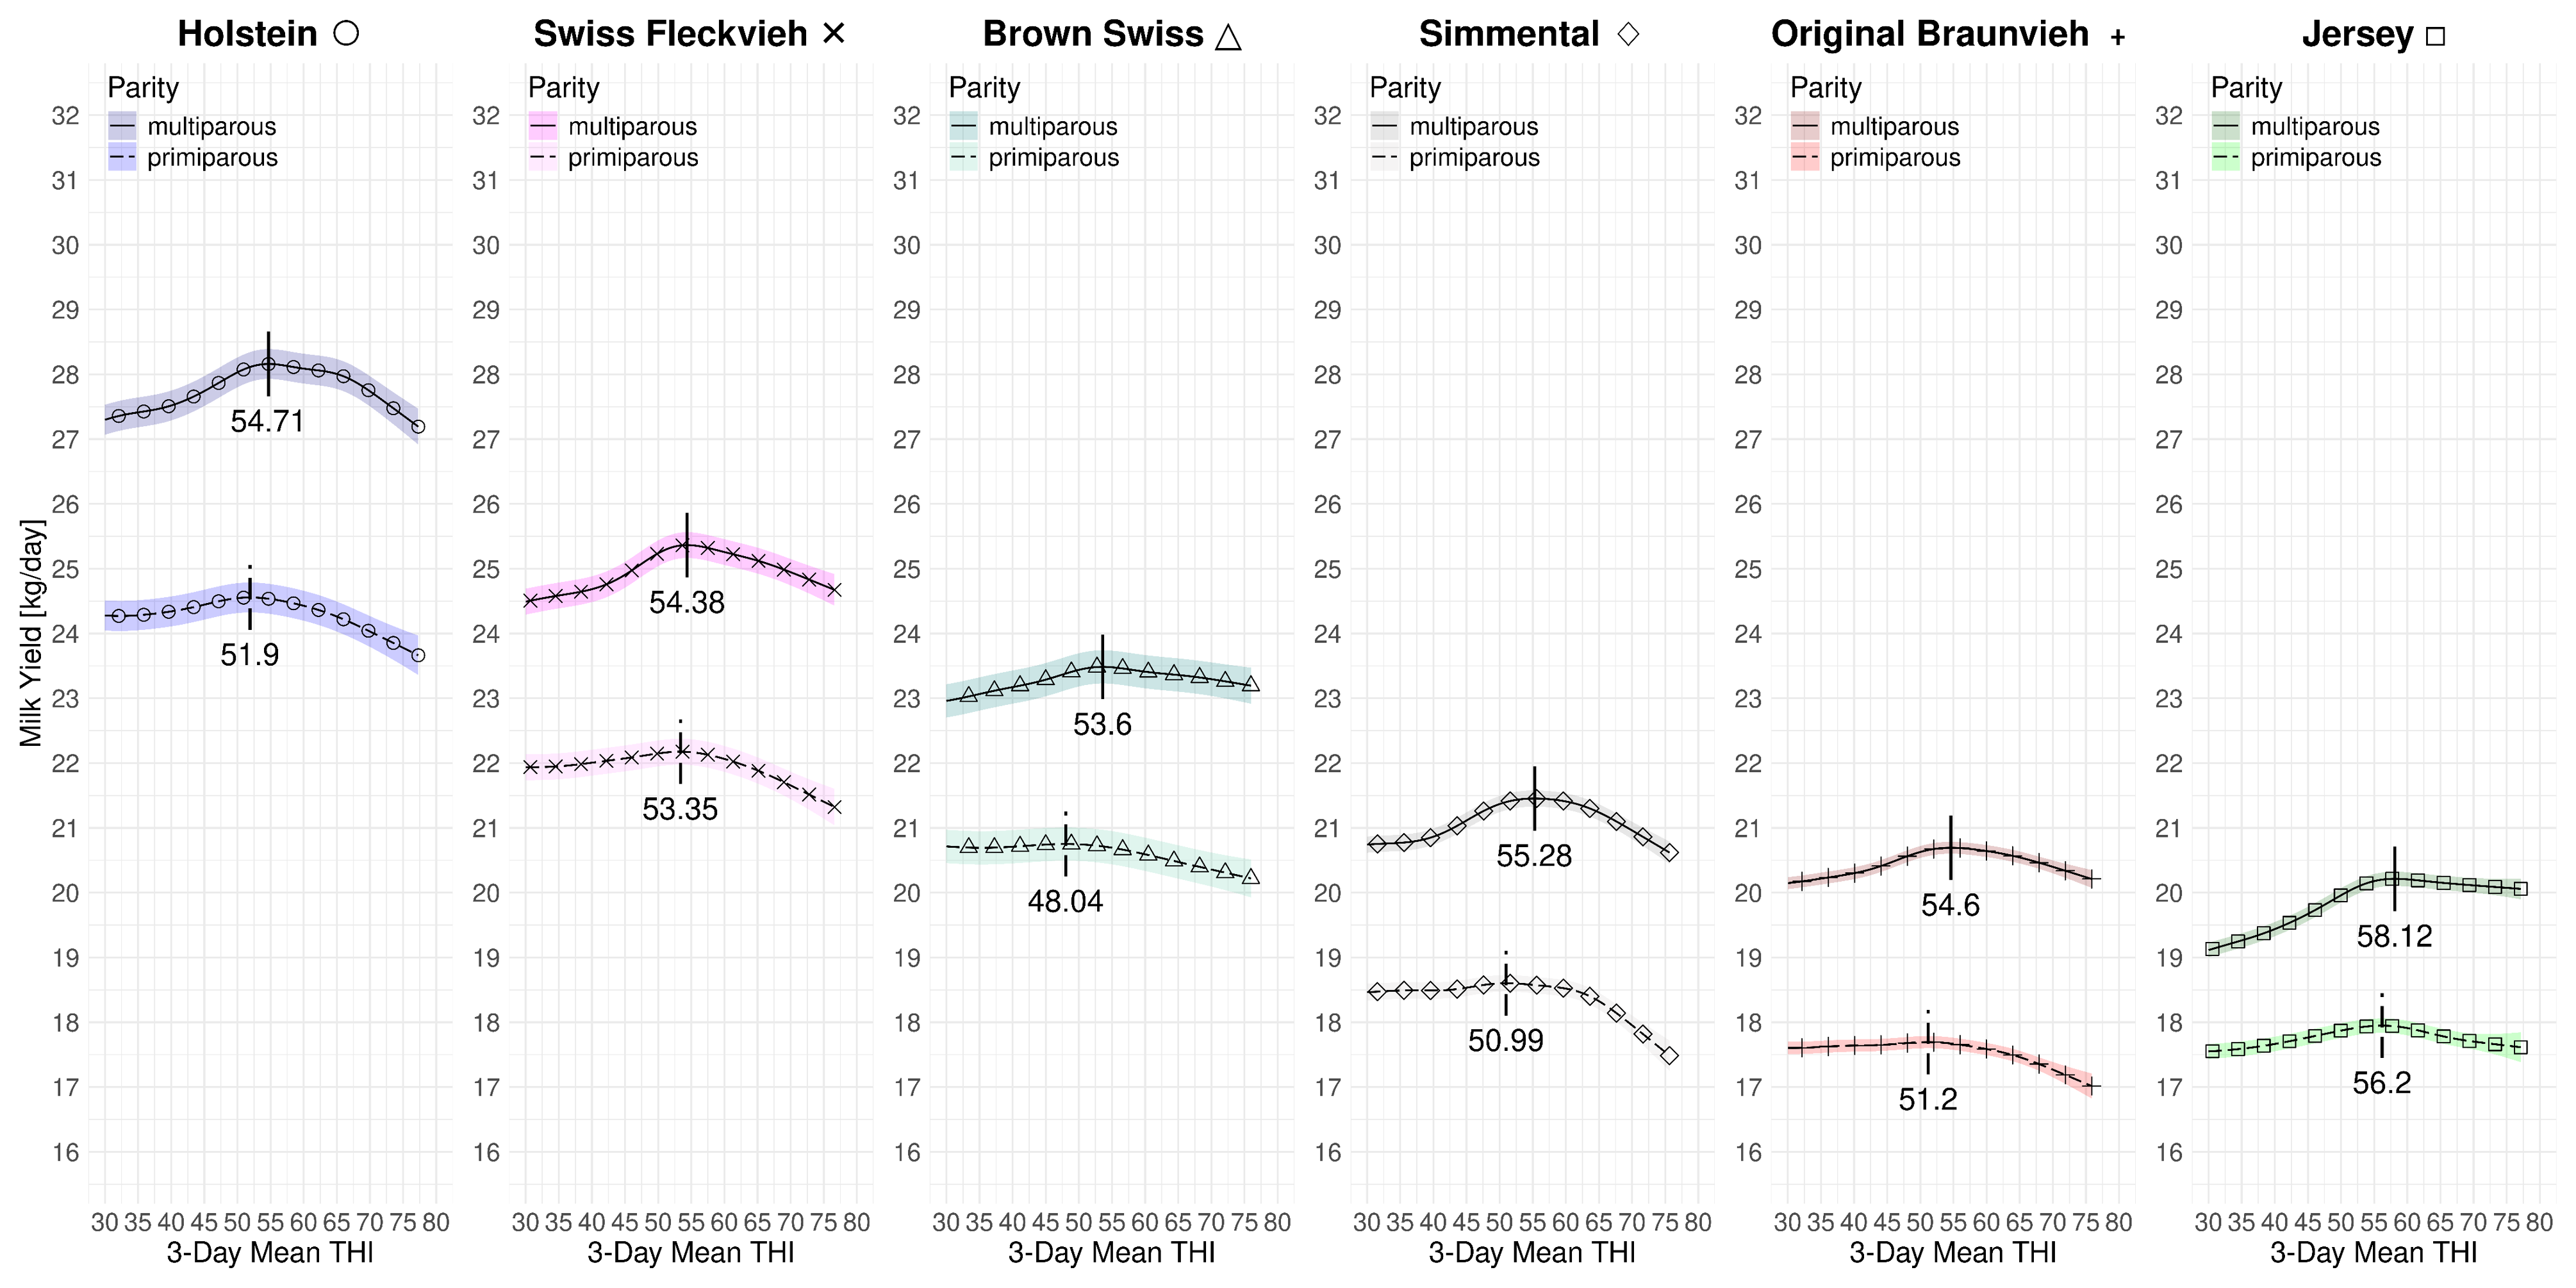
\includegraphics[width=0.85\paperheight]{thesis/figures/results/milk_yield.png}
    
    \caption{3-day mean THI effect on milk yield for primi- and multiparous Swiss dairy cows at 2023 levels with data subsamples covering the full time period from 1983-2023.}
    \label{fig:results_milk_yield}
\end{figure}
\begin{textblock*}{2cm}(20cm, \dimexpr\paperheight/2)
  \rotatebox{90}{\thepage}
\end{textblock*}
\end{landscape}
\newpage
Figure~\ref{fig:results_milk_yield} summarizes the effect of the 3-day mean THI on the volumetric milk yield for both parities and all breeds at average 2023 levels. The subplots are in descending order with respect to the average yields with the high-yield Holstein yield on the left and the modest-yield Jersey breed on the right. Table~\ref{table:milk_yield_full_period} provides a summary of the THI turning points and the associated loss rates. For multiparous cows the peak THI points range from 53.6 for Brown Swiss to 58.12 for Jersey. The THI difference between the lowest and highest peak point is 4.56 THI points. For primiparous cows the the lowest THI peak point is 48.04 for Brown Swiss and 56.2 for Jersey. The THI difference between the lowest and highest peak point for primiparous cows is 8.16 points. In both cases, for Brown Swiss and Jersey, the curves for primi- and multiparous cows, the marginal losses are less accentuated than for the other breeds. For primiparous Simmental we observe a steep drop after a relatively stable period beyond the THI turning point. Figure~\ref{fig:results_milk_marginal_parimiprous} and Figure~\ref{fig:results_milk_marginal_multiparous} only depict the marginal effects of THI without adding the average levels of year and parity. We observe a two-stage decrease for multiparous Holsteins: similarly as for primiparous Simmental, the milk yield decline starts at a THI of 54.71 at a moderate rate. Then, at an approximate value of 65, the loss rate is more steep.

\begin{table}[htbp]
    \centering
    % Define 12 columns
    \begin{tabular}{c c c c c c c c c c c c}
        \toprule
        % First header row
        \multirow{2}{*}{Details} &
        \multirow{2}{*}{\textbf{Breed}} &
        \multirow{2}{*}{\textbf{Period}} &
        \multicolumn{2}{c}{\textbf{THI Peak}} &
        \multicolumn{2}{c}{\textbf{DIM Peak}} &
        \multicolumn{2}{c}{\textbf{THI Loss Rate}} &
        \multicolumn{2}{c}{$\mathbf{R^2}$} \\
        \cmidrule(lr){4-5} \cmidrule(lr){6-7} \cmidrule(lr){8-9} \cmidrule(lr){10-11}
        % Second header row
        & & &
        \textbf{P} & \textbf{M} &
        \textbf{P} & \textbf{M} &
        \textbf{P} & \textbf{M} &
        $\mathbf{R^2_m}$ & $\mathbf{R^2_c}$ & \\
        \hline
        \hline
        % Data rows (replace with your actual data)
        \textcolor{blue}{\ref{model:ho_milk_full}}& HO & Full & 51.90 & 54.71 & 37 & 31 & -0.035 & -0.043 & 0.12 & 0.95\\
        \textcolor{blue}{\ref{model:sf_milk_full}}& SF & Full & 53.35 & 54.38 & 30 & 25 & -0.037 & -0.031 & 0.07 & 0.93\\
        \textcolor{blue}{\ref{model:bs_milk_full}}& BS & Full & 48.04 & 53.60 & 21 & 20 & -0.019 & -0.013 & 0.10 & 0.95\\
        \textcolor{blue}{\ref{model:si_milk_full}}& SI & Full & 50.99 & 55.28 & 26 & 21 & -0.045 & -0.041 & 0.04 & 0.94\\
        \textcolor{blue}{\ref{model:ob_milk_full}}& OB & Full & 51.20 & 54.60 & 24 & 20 & -0.027 & -0.023 & 0.07 & 0.96\\
        \textcolor{blue}{\ref{model:je_milk_full}}& JE & Full & 56.20 & 58.12 & 31 & 25 & -0.016 & -0.008 & 0.14 & 0.95\\
        % Add more data rows as needed
        \bottomrule
    \end{tabular}
    \caption{Milk Yield - Full Period - Turning Points and Loss Rates}
    \label{table:milk_yield_full_period}
\end{table}

\begin{figure}[H]
    \centering
    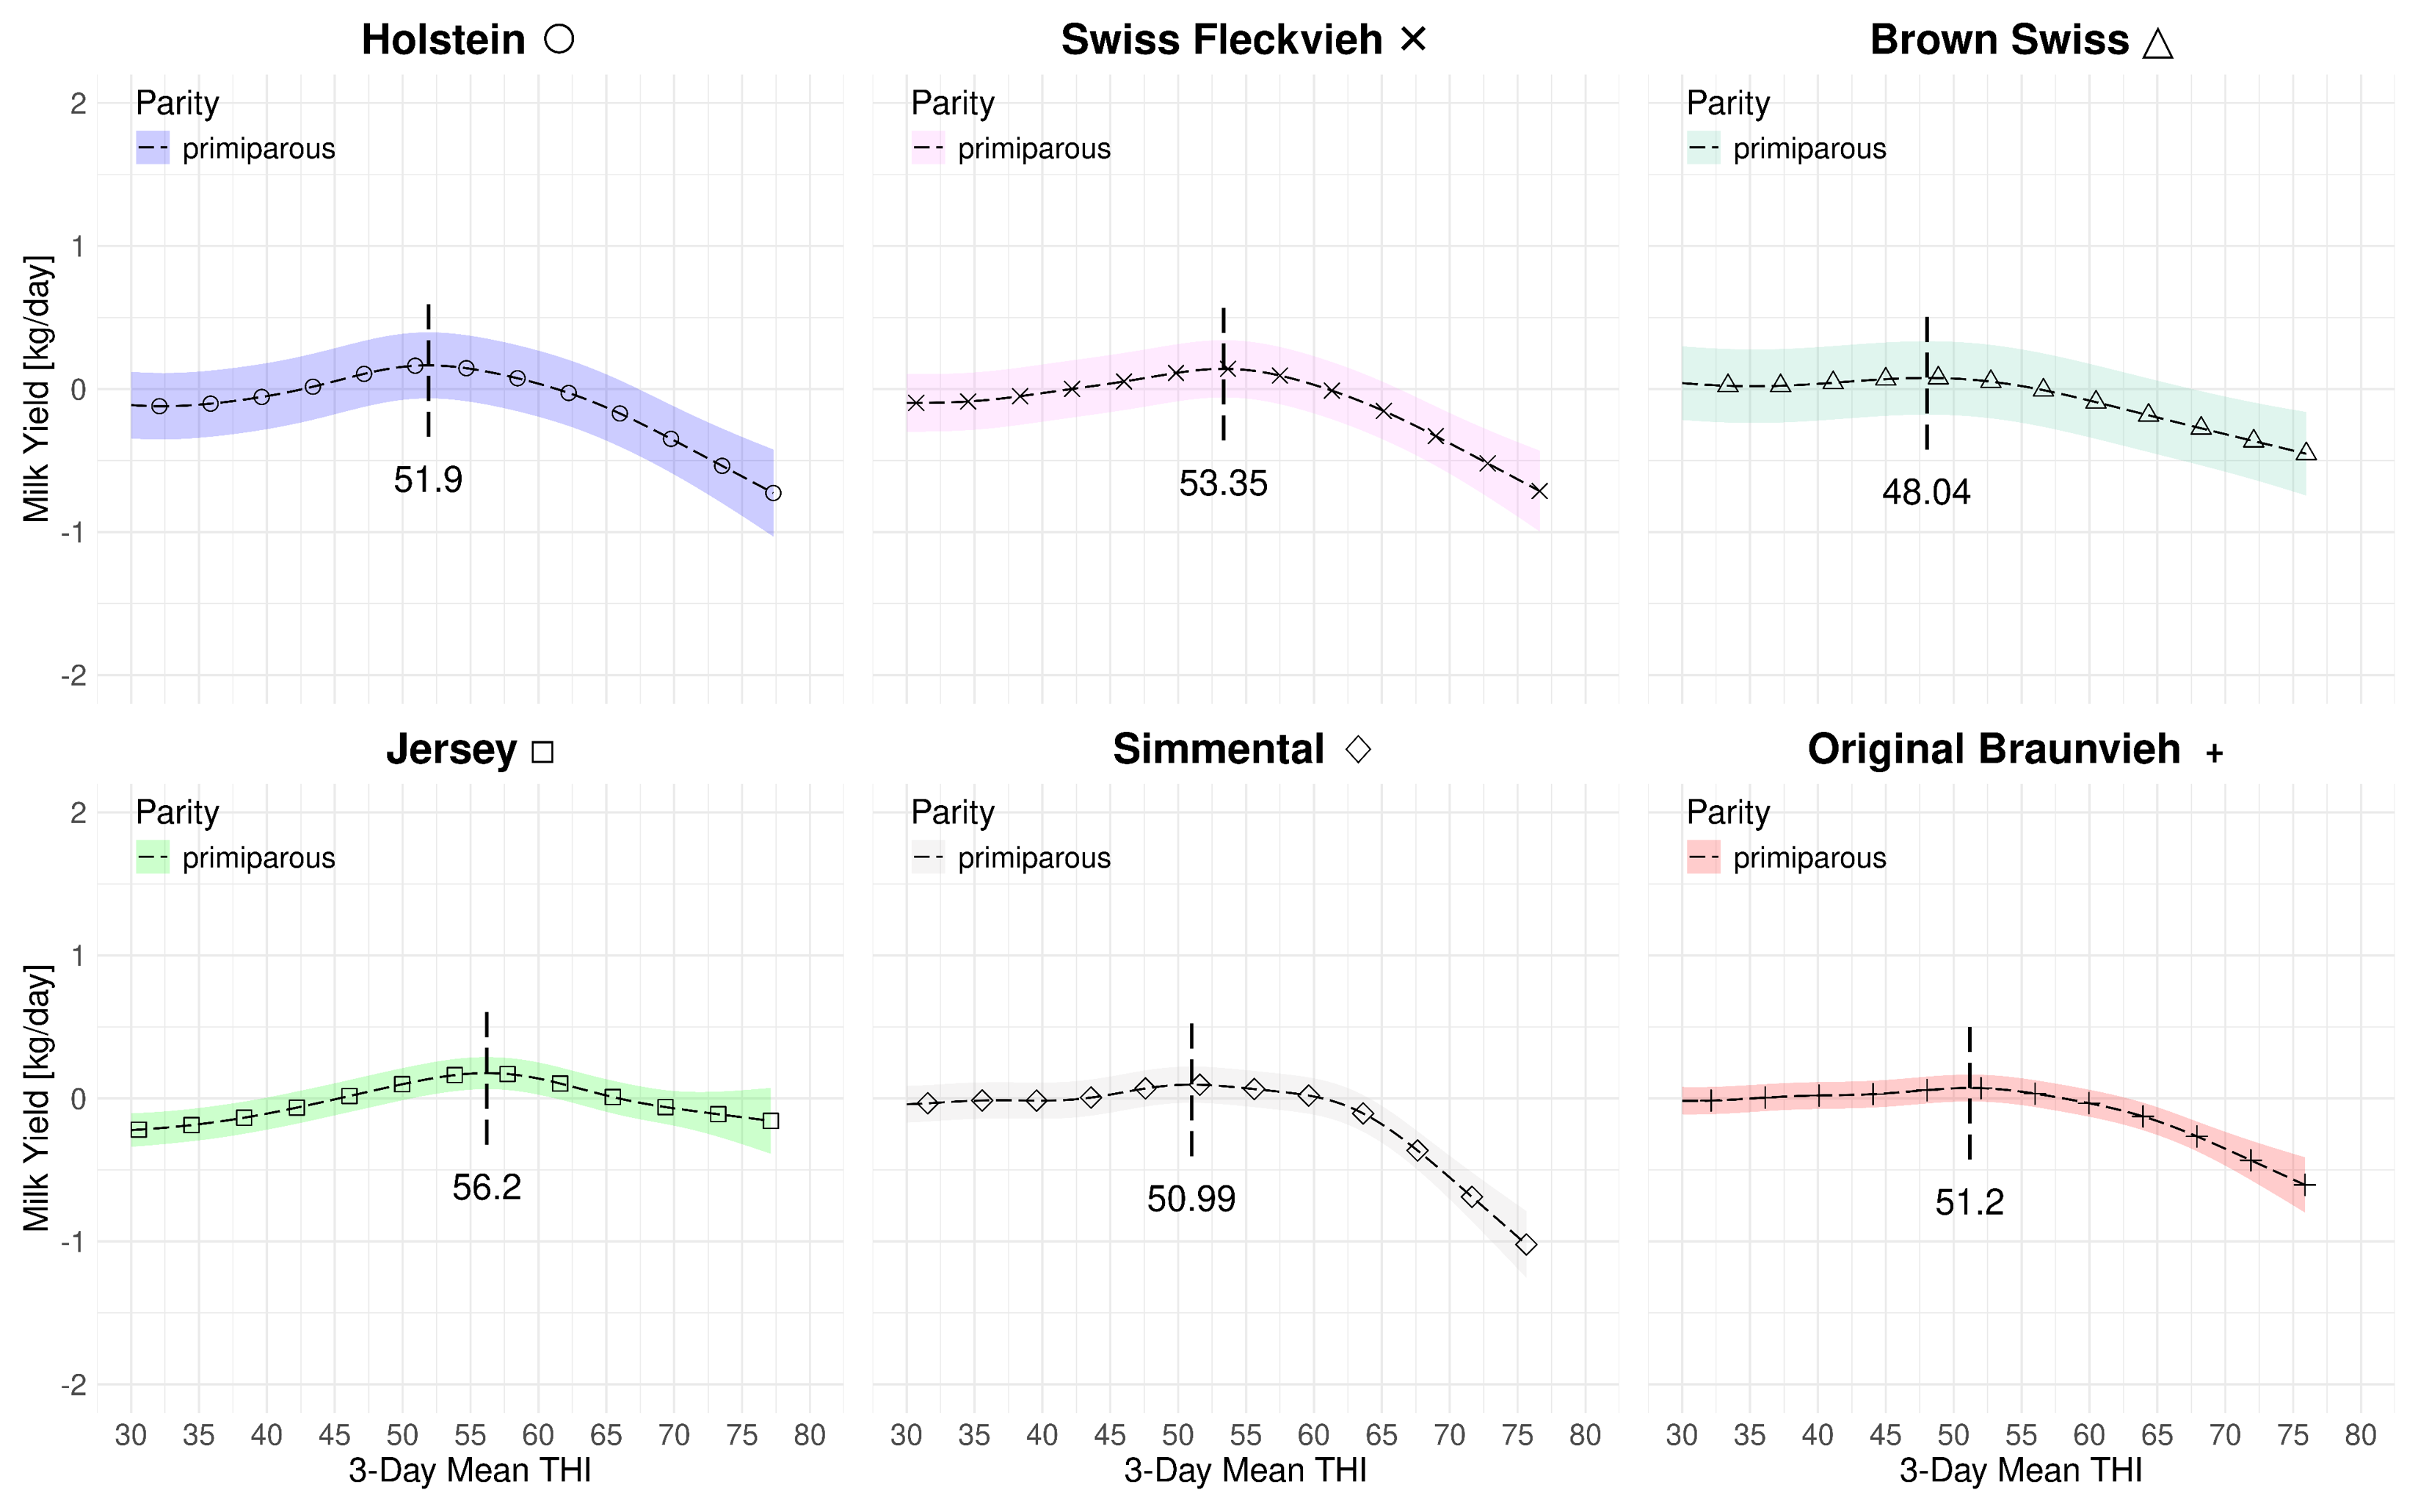
\includegraphics[width=\textwidth]{thesis/figures/results/milk_yield_marginal_primi.png}
    \caption{3-day mean marginal THI effect on milk yield for primiparous Swiss dairy cows at 2023 levels with data subsamples covering the full time period from 1982-2023.}
    \label{fig:results_milk_marginal_parimiprous}
\end{figure}

\begin{figure}[H]
    \centering
    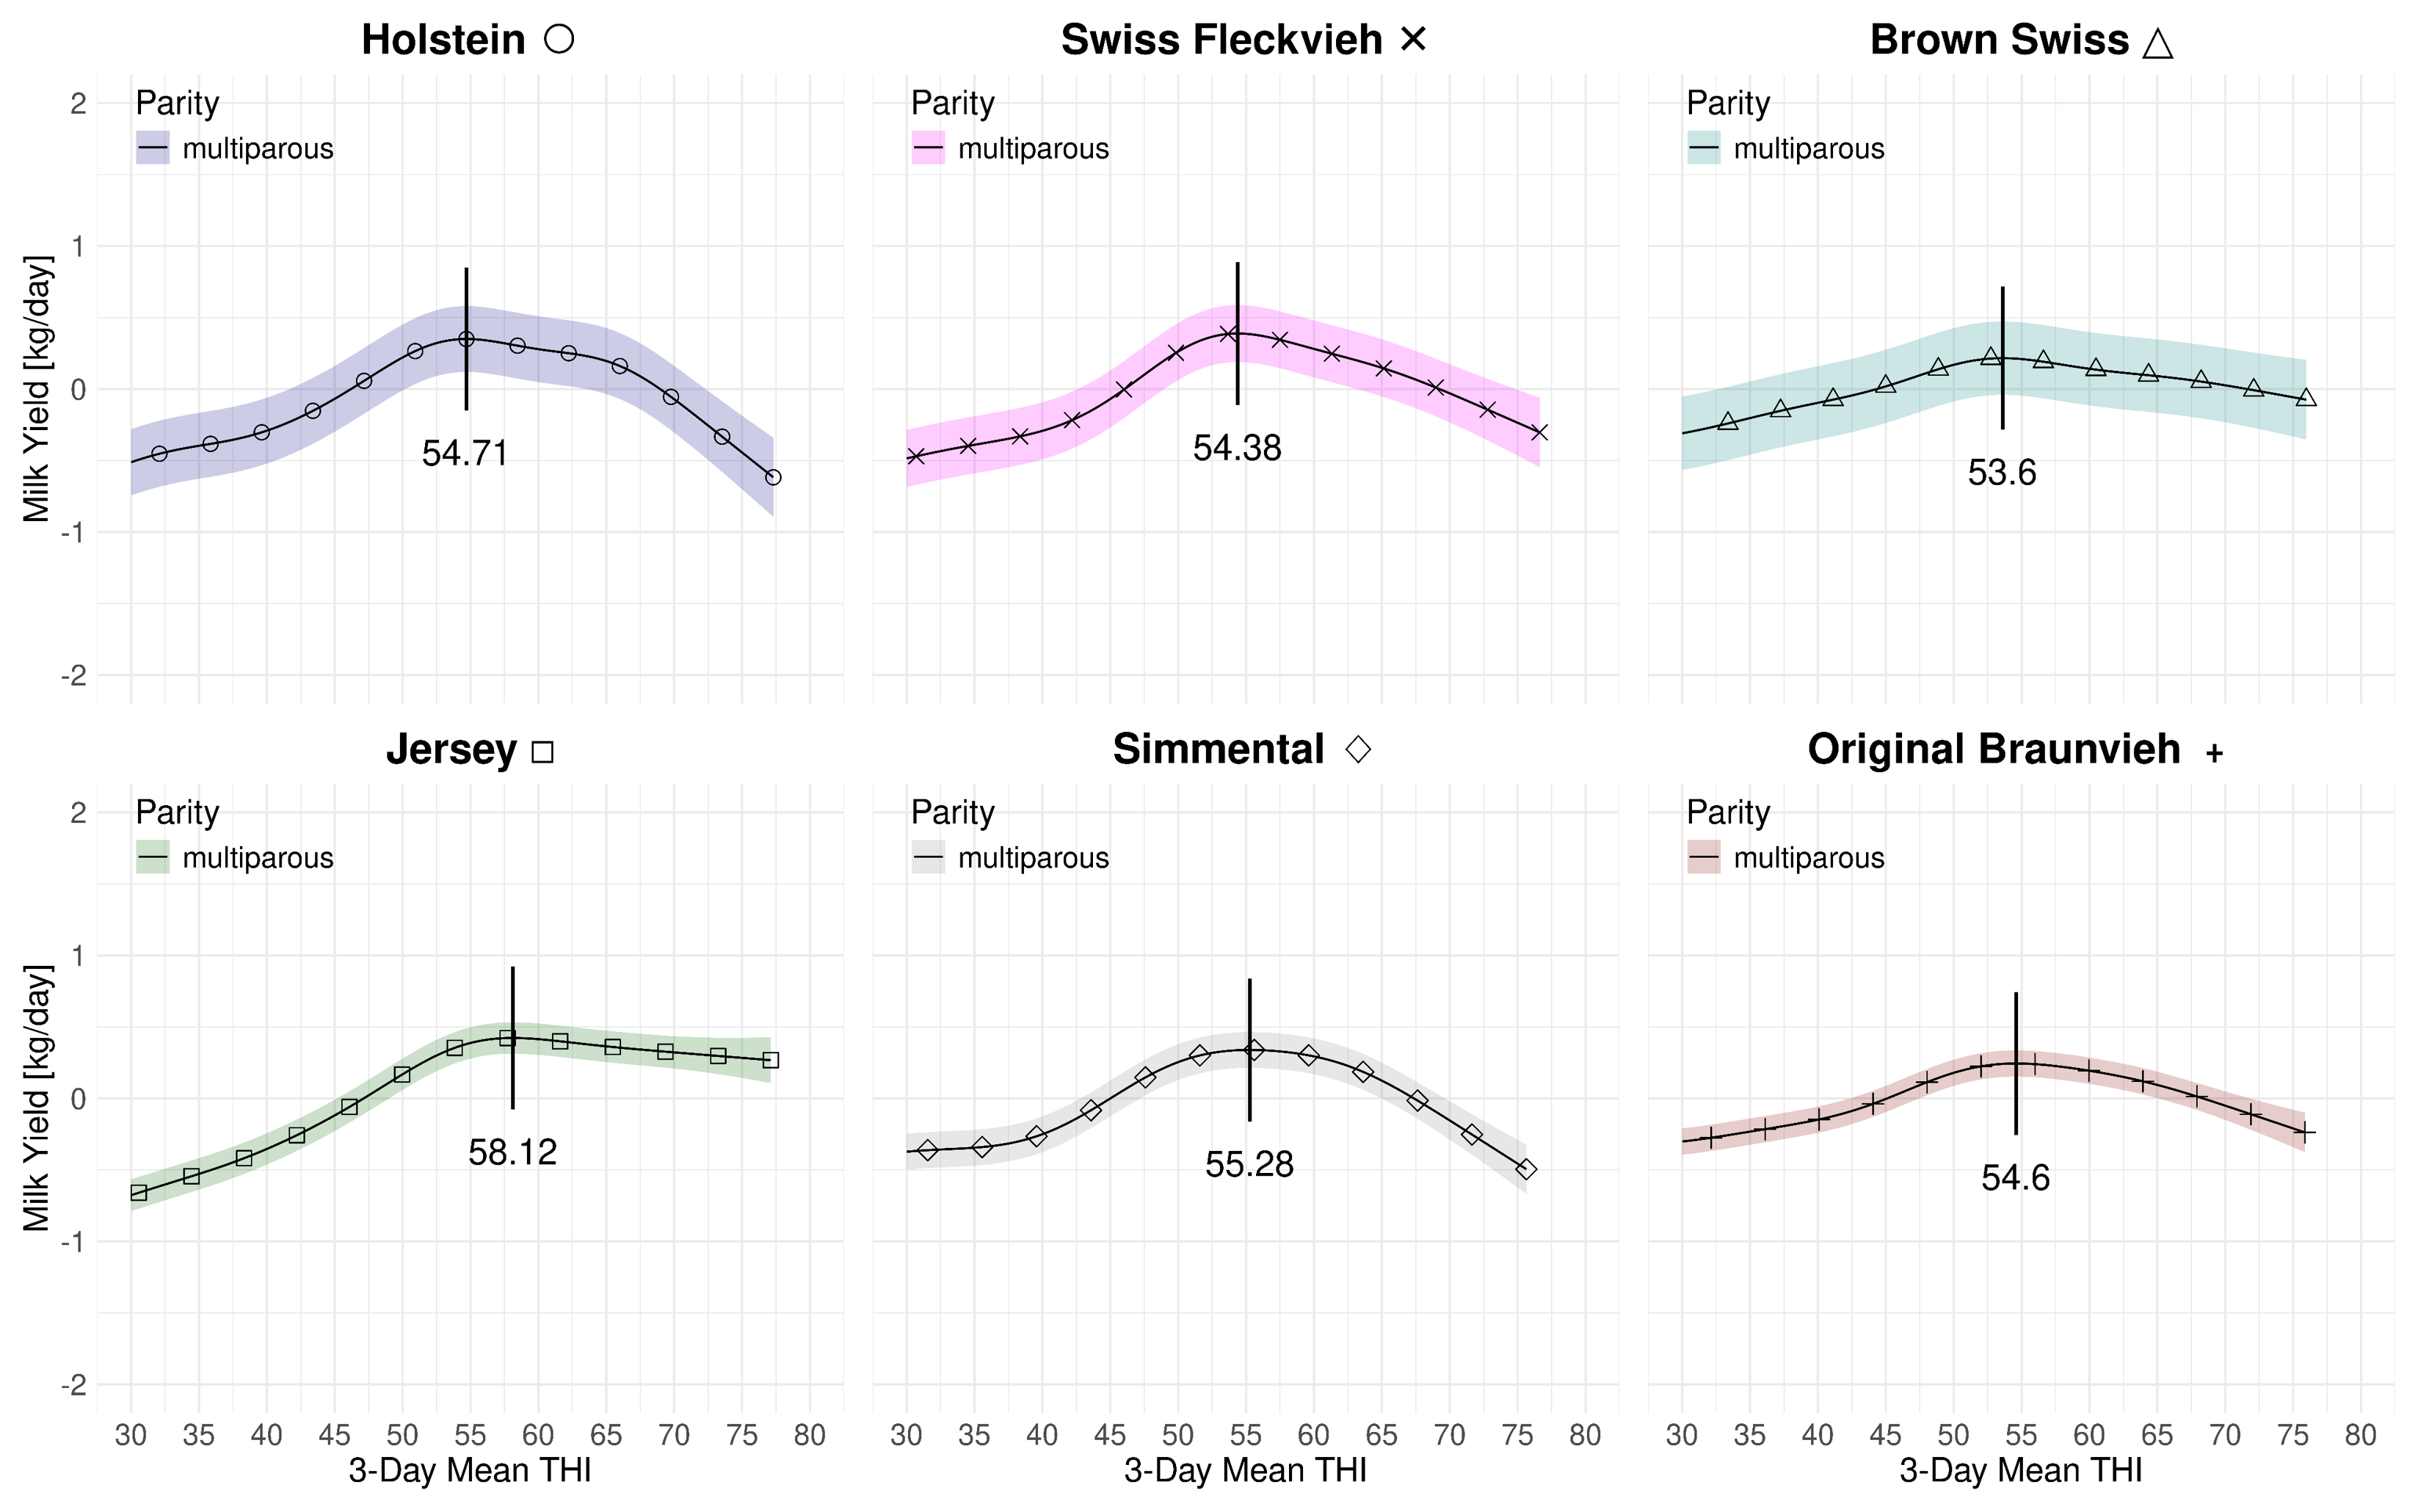
\includegraphics[width=\textwidth]{thesis/figures/results/milk_yield_marginal_multi.png}
    
    \caption{3-day mean marginal THI effect on milk yield for multiparous Swiss dairy cows at 2023 levels with data subsamples covering the full time period from 1982-2023.}
    \label{fig:results_milk_marginal_multiparous}
\end{figure}


    
\newpage

\newpage
\begin{landscape}
    \thispagestyle{empty}
    \section{ECM Yield}\label{sec:ecm_yield}
    \begin{figure}[ht]
        \centering
        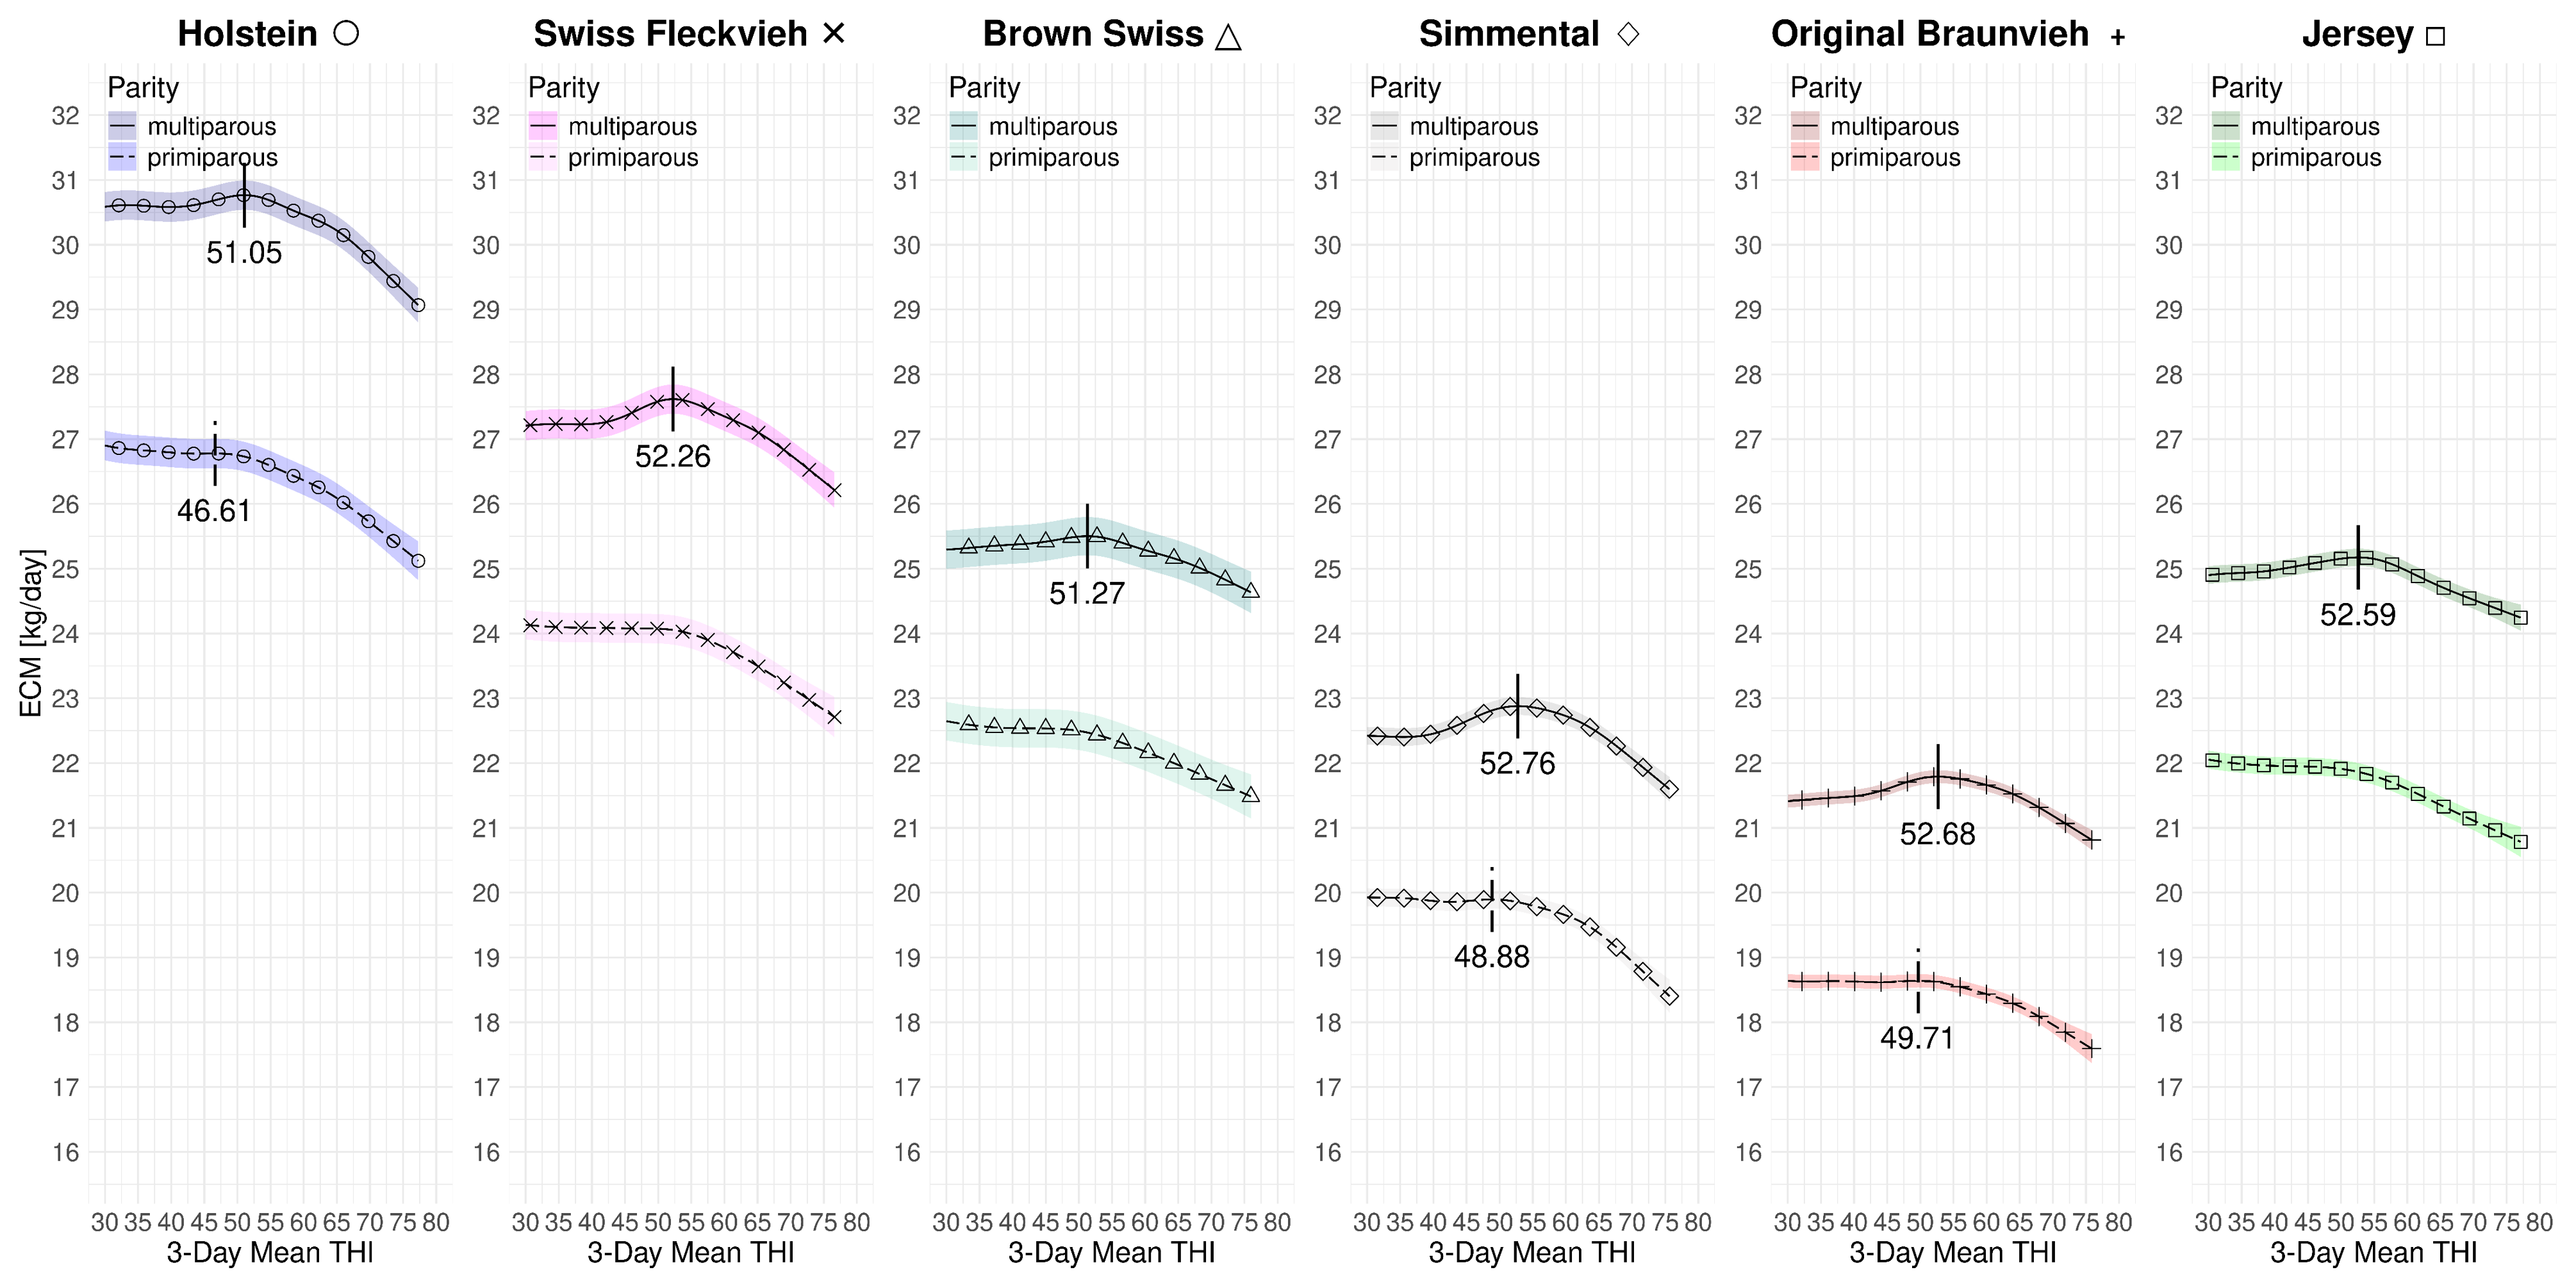
\includegraphics[width=0.85\paperheight]{thesis/figures/results/ecm_yield.png}
        \caption{3-day mean THI effect on ECM yield for primi- and multiparous Swiss dairy cows at 2023 levels with data subsamples covering the full time period from 1983-2023.}
        \label{fig:results_ecm_yield}
    \end{figure}
    
    \begin{textblock*}{2cm}(20cm, \dimexpr\paperheight/2)
    \rotatebox{90}{\thepage}
    \end{textblock*}
\end{landscape}
\newpage


Figure~\ref{fig:results_ecm_yield} summarizes the effect of the 3-day mean THI on the component-corrected milk yield for both parities and all breeds at average 2023 levels. Hence, the milk yield is normalized with respect to fat and protein. First, by the definition of ECM, the average yield levels increase for all breeds\footnote{The average milk and ECM yield levels of 2023 derived with descriptive statistics can be consulted in Table~\ref{table:average_breed_performance_2023}}. The jump for Jersey cows is expected since they are known as a high-fat and high-protein breed. Moreover, we are able to identify turning points for all breeds in the multiparous case. The lowest THI peak is at 51.05 for Holstein and the highest at 52.76 for Simmental. The difference between the lowest and highest THI peak point is 1.71. For primiparous cows, we cannot identify the THI turning points for Swiss Fleckvieh, Brown Swiss and Jersey. This is because their corresponding slopes are continuously decreasing. Therefore, from a numerical perspective, there are no turning points in these cases. However, in all three cases, fairly steep changes in the loss rates at THI values in the mid-fifties are identifiable. For the other three breeds with available turning points, these are Holstein (46.61), Simmental (48.88) and Original Braunvieh (49.71). Among them, the difference between the lowest and highest turning point is 3.41 THI points. Table~\ref{table:ecm_yield_full_period} lists the individual THI turning points. Figure~\ref{fig:results_ecm_marginal_parimiprous} and Figure~\ref{fig:results_ecm_marginal_multiparous} solely visualize the marginal effects of THI on ECM yield in separate subfigures for primi- and multiparous cows.

\begin{table}[htbp]
    \centering
    % Define 12 columns
    \begin{tabular}{c c c c c c c c c c c c}
        \toprule
        % First header row
        \multirow{2}{*}{Details} &
        \multirow{2}{*}{\textbf{Breed}} &
        \multirow{2}{*}{\textbf{Period}} &
        \multicolumn{2}{c}{\textbf{THI Peak}} &
        \multicolumn{2}{c}{\textbf{DIM Peak}} &
        \multicolumn{2}{c}{\textbf{THI Loss Rate}} &
        \multicolumn{2}{c}{$\mathbf{R^2}$} \\
        \cmidrule(lr){4-5} \cmidrule(lr){6-7} \cmidrule(lr){8-9} \cmidrule(lr){10-11}
        % Second header row
        & & &
        \textbf{P} & \textbf{M} &
        \textbf{P} & \textbf{M} &
        \textbf{P} & \textbf{M} &
        $\mathbf{R^2_m}$ & $\mathbf{R^2_c}$ & \\
        \hline
        \hline
        % Data rows (replace with your actual data)
        \textcolor{blue}{\ref{model:ho_ecm_full}}& HO & Full & 46.61 & 51.05 & 13 & 20 & -0.054 & -0.065 & 0.06 & 0.89\\
        \textcolor{blue}{\ref{model:sf_ecm_full}}& SF & Full & - & 52.26 & 11 & - & - & -0.058 & 0.07 & 0.90\\
        \textcolor{blue}{\ref{model:bs_ecm_full}}& BS & Full & - & 51.27 & 13 & 8 & - & -0.035 & 0.06 & 0.92\\
        \textcolor{blue}{\ref{model:si_ecm_full}}& SI & Full & 48.88 & 52.76 & 9 & - & -0.056 & -0.056 & 0.03 & 0.93\\
        \textcolor{blue}{\ref{model:ob_ecm_full}}& OB & Full & 49.71 & 52.68 & 14 & 4 & -0.042 & -0.040 & 0.04 & 0.92\\
        \textcolor{blue}{\ref{model:je_ecm_full}}& JE & Full & - & 52.59 & 22 & 23 & - & -0.038 & 0.07 & 0.90\\
        % Add more data rows as needed
        \bottomrule
    \end{tabular}
    \caption{ECM Yield - Full Period - Turning Points and Loss Rates}
    \label{table:ecm_yield_full_period}
\end{table}

\begin{figure}[H]
    \centering
    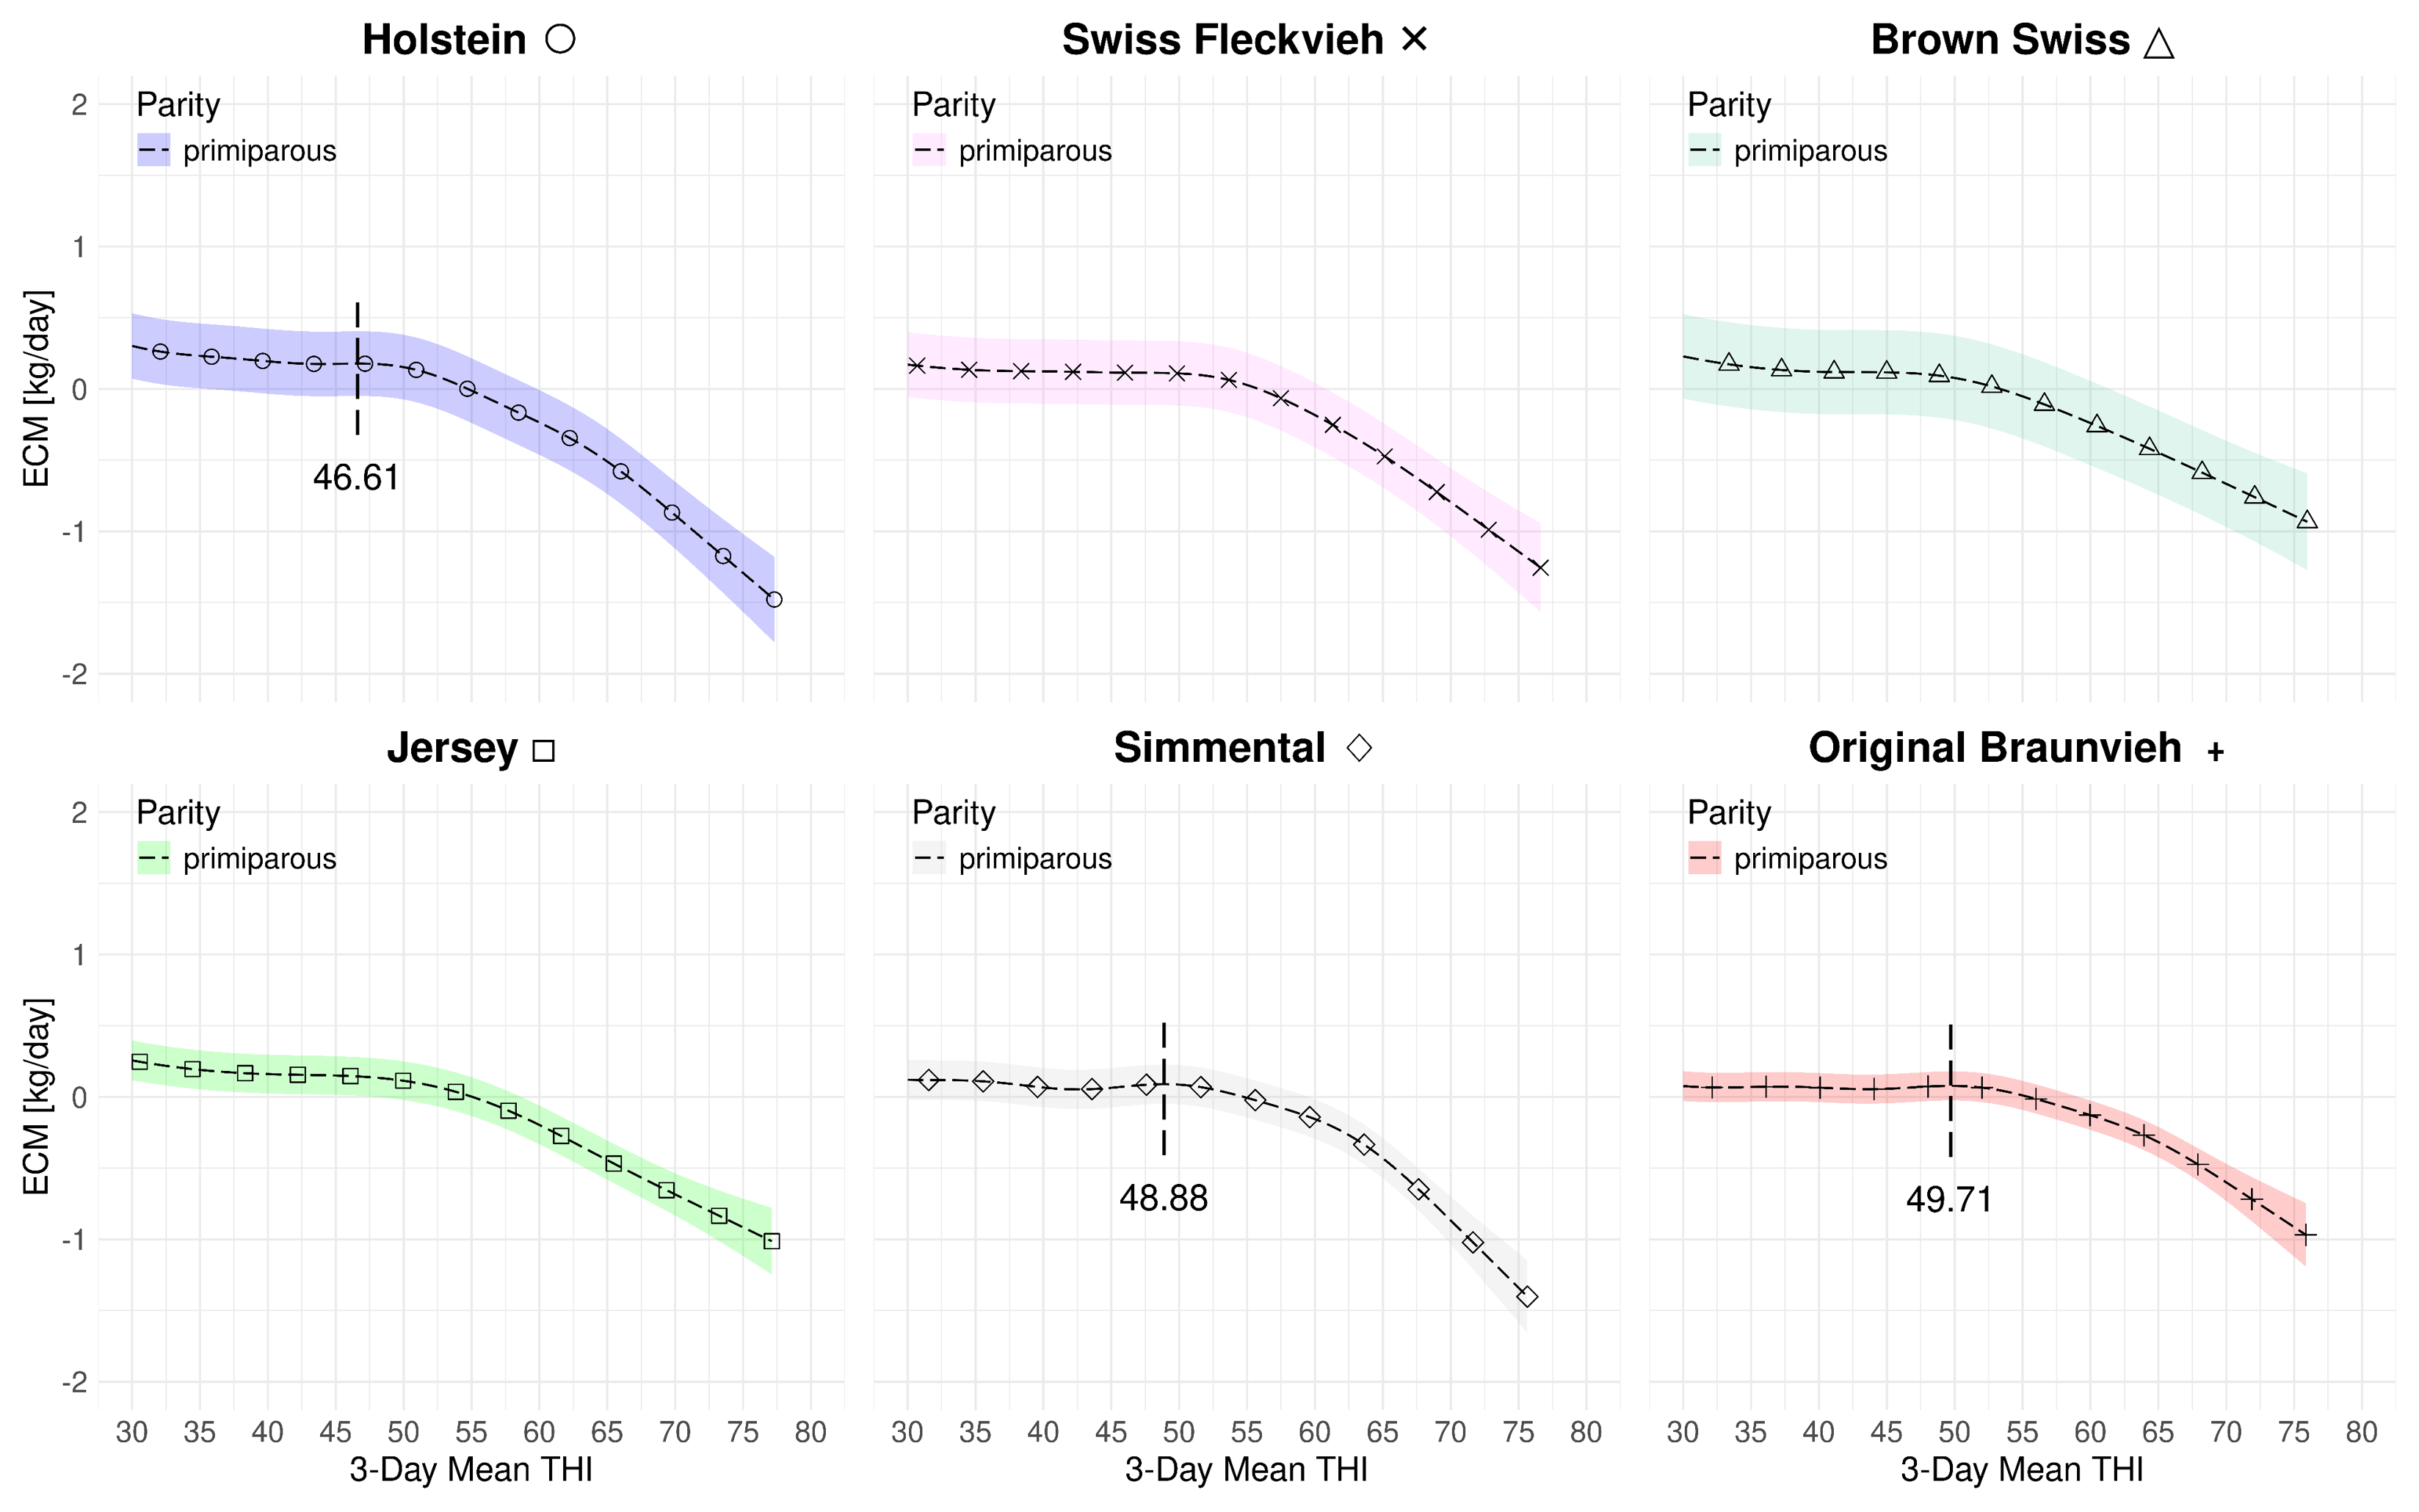
\includegraphics[width=\textwidth]{thesis/figures/results/ecm_yield_marginal_primi.png}
    \caption{3-day mean marginal THI effect on ECM yield for primiparous Swiss dairy cows at 2023 levels with data subsamples covering the full time period from 1983-2023.}
    \label{fig:results_ecm_marginal_parimiprous}
\end{figure}

\begin{figure}[H]
    \centering
    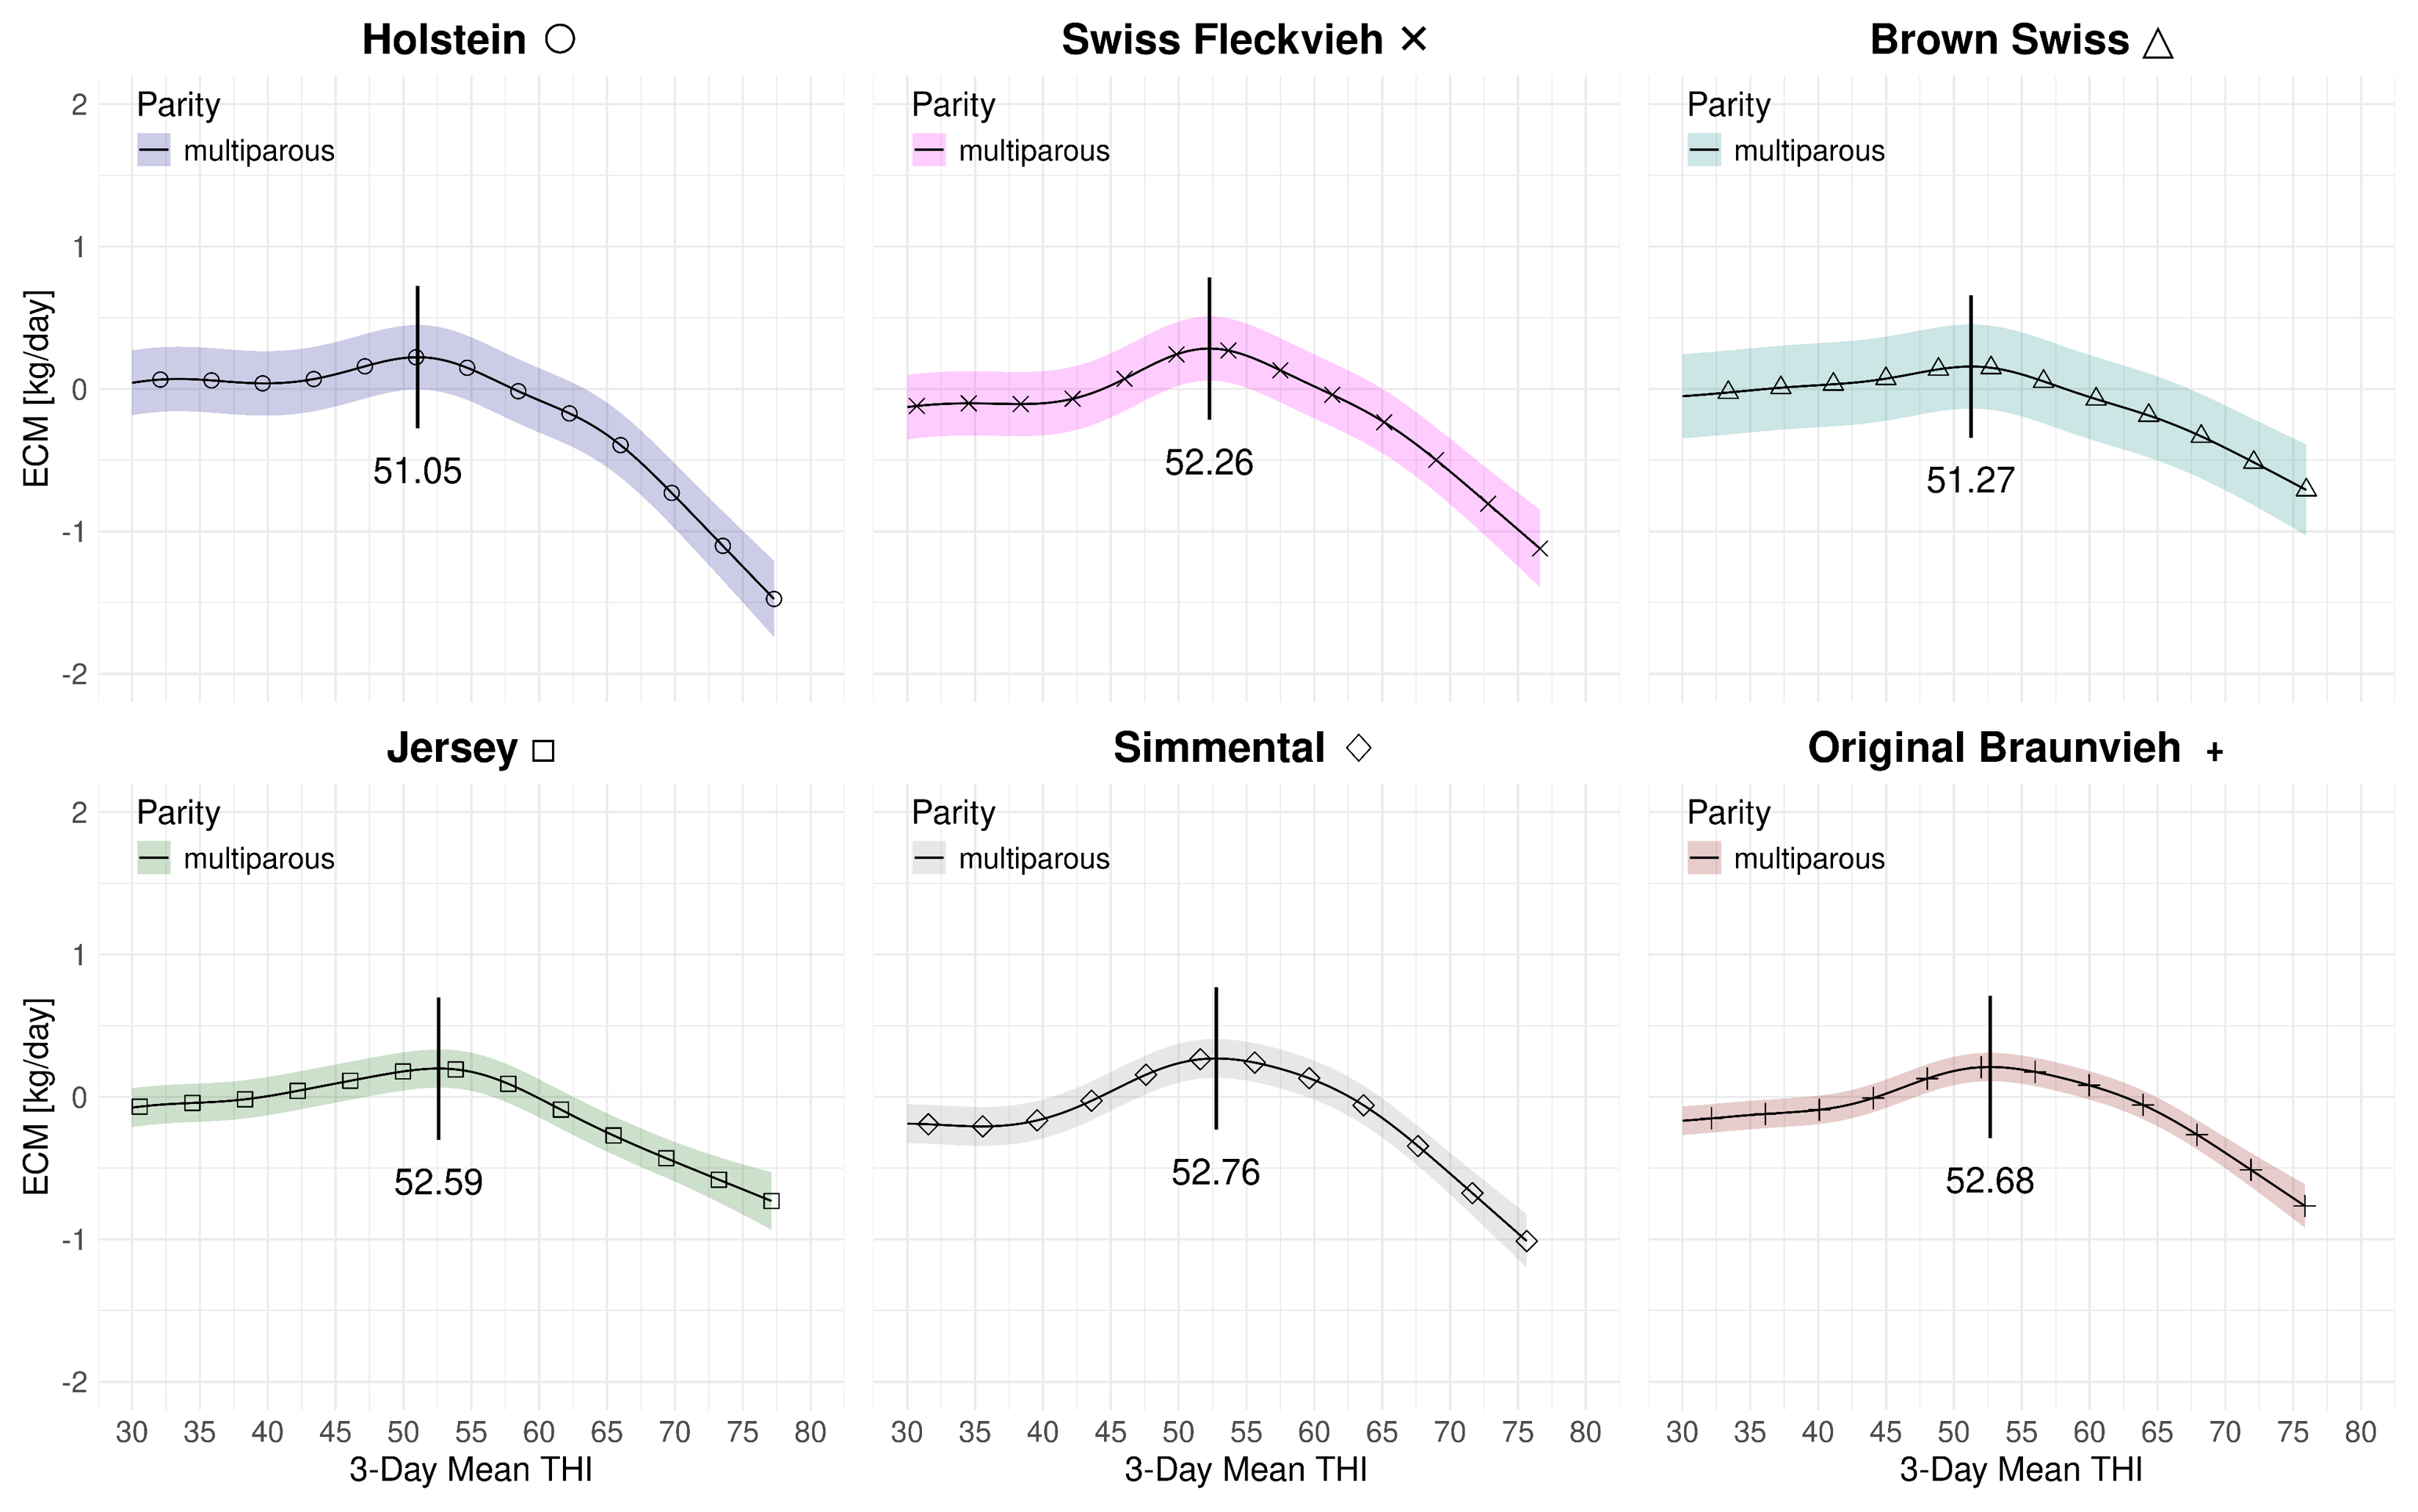
\includegraphics[width=\textwidth]{thesis/figures/results/ecm_yield_marginal_multi.png}
    
    \caption{3-day mean marginal THI effect on ECM yield for multiparous Swiss dairy cows at 2023 levels with data subsamples covering the full time period from 1983-2023.}
    \label{fig:results_ecm_marginal_multiparous}
\end{figure}



\newpage

\section{Split Period: Until 2010 - After 2010}\label{sec:split_period}
Table~\ref{table:milk_yield_split_period} and Table~\ref{table:ecm_yield_split_period} compare the THI turning points and loss rates for the split-period experiments. The associated figures are provided in Appendix~\ref{appendix:split_period}. We observe THI turning point shifts between the two periods. More specifically, the turning points are at lower THI values in the period 2011-2023. However, in many cases, leftward turning point shifts, come with lower linearized loss rates.

% Second Table
\begin{table}[htbp]
    \centering
    % Define 12 columns
    \begin{tabular}{c c c c c c c c c c c c}
        \toprule
        % First header row
        \multirow{2}{*}{Details} &
        \multirow{2}{*}{\textbf{Breed}} &
        \multirow{2}{*}{\textbf{Period}} &
        \multicolumn{2}{c}{\textbf{THI Peak}} &
        \multicolumn{2}{c}{\textbf{DIM Peak}} &
        \multicolumn{2}{c}{\textbf{THI Loss Rate}} &
        \multicolumn{2}{c}{$\mathbf{R^2}$} \\
        \cmidrule(lr){4-5} \cmidrule(lr){6-7} \cmidrule(lr){8-9} \cmidrule(lr){10-11}
        % Second header row
        & & &
        \textbf{P} & \textbf{M} &
        \textbf{P} & \textbf{M} &
        \textbf{P} & \textbf{M} &
        $\mathbf{R^2_m}$ & $\mathbf{R^2_c}$ & \\
        \hline
        \hline
        % Data rows (replace with your actual data)
        \textcolor{blue}{\ref{model:ho_milk_before}}& HO & $\leq 2010$ & 53.40 & 55.24 & 35 & 28 & -0.040 & -0.041 & 0.06 & 0.94\\
        \textcolor{blue}{\ref{model:ho_milk_after}}& HO & $>2010$ & 51.19 & 54.83 & 37 & 33 & -0.031 & -0.040 & 0.12 & 0.95\\
        \hline
        \textcolor{blue}{\ref{model:sf_milk_before}}& SF & $\leq 2010$ & 54.00 & 54.34 & 29 & 24 & -0.033 & -0.033 & 0.05 & 0.93\\
        \textcolor{blue}{\ref{model:sf_milk_after}}& SF & $>2010$ & 51.75 & 54.62 & 35 & 28 & -0.023 & -0.010 & 0.07 & 0.94\\
        \hline
        \textcolor{blue}{\ref{model:bs_milk_before}}& BS & $\leq 2010$ & 52.40 & 53.67 & 21 & 20 & -0.024 & -0.028 & 0.08 & 0.95\\
        \textcolor{blue}{\ref{model:bs_milk_after}}& BS & $>2010$ & 46.76 & 51.83 & 26 & 22 & -0.021 & -0.006 & 0.10 & 0.95\\
        \hline
        \textcolor{blue}{\ref{model:si_milk_before}}& SI & $\leq 2010$ & 52.26 & 55.80 & 25 & 20 & -0.034 & -0.026 & 0.03 & 0.93\\
        \textcolor{blue}{\ref{model:si_milk_after}}& SI & $>2010$ & 53.10 & 55.35 & 28 & 22 & -0.023 & -0.013 & 0.03 & 0.94\\
        \hline
        \textcolor{blue}{\ref{model:ob_milk_before}}& OB & $\leq 2010$ & 52.73 & 55.01 & 23 & 20 & -0.028 & -0.025 & 0.04 & 0.95\\
        \textcolor{blue}{\ref{model:ob_milk_after}}& OB & $>2010$ & 49.49 & 52.63 & 29 & 21 & -0.023 & -0.019 & 0.06 & 0.94\\
        \hline
        \textcolor{blue}{\ref{model:je_milk_before}}& JE & $\leq 2010$ & 57.09 & 58.33 & 27 & 22 & -0.019 & -0.021 & 0.10 & 0.96\\
        \textcolor{blue}{\ref{model:je_milk_after}}& JE & $>2010$ & 55.06 & 58.13 & 33 & 27 & -0.015 & -0.007 & 0.12 & 0.95\\            
        % Add more data rows as needed
        \bottomrule
    \end{tabular}
    \caption{Milk Yield - Split Period - Turning Points and Loss Rates}
    \label{table:milk_yield_split_period}
\end{table}

% Second Table
\begin{table}[htbp]
    \centering
    % Define 12 columns
    \begin{tabular}{c c c c c c c c c c c c}
        \toprule
        % First header row
        \multirow{2}{*}{Details} &
        \multirow{2}{*}{\textbf{Breed}} &
        \multirow{2}{*}{\textbf{Period}} &
        \multicolumn{2}{c}{\textbf{THI Peak}} &
        \multicolumn{2}{c}{\textbf{DIM Peak}} &
        \multicolumn{2}{c}{\textbf{THI Loss Rate}} &
        \multicolumn{2}{c}{$\mathbf{R^2}$} \\
        \cmidrule(lr){4-5} \cmidrule(lr){6-7} \cmidrule(lr){8-9} \cmidrule(lr){10-11}
        % Second header row
        & & &
        \textbf{P} & \textbf{M} &
        \textbf{P} & \textbf{M} &
        \textbf{P} & \textbf{M} &
        $\mathbf{R^2_m}$ & $\mathbf{R^2_c}$ & \\
        \hline
        \hline
        % Data rows (replace with your actual data)
        
        \textcolor{blue}{\ref{model:ho_ecm_before}}& HO & $\leq 2010$ & 48.48 & 51.40 & 15 & - & -0.057 & -0.060 & 0.07 & 0.88\\
        \textcolor{blue}{\ref{model:ho_ecm_after}}& HO & $>2010$ & 47.49 & 50.05 & 23 & 15 & -0.054 & -0.059 & 0.06 & 0.89\\
        \hline
        \textcolor{blue}{\ref{model:sf_ecm_before}}& SF & $\leq 2010$ & 50.05 & 52.27 & - & - & -0.047 & -0.059 & 0.06 & 0.90\\
        \textcolor{blue}{\ref{model:sf_ecm_after}}& SF & $>2010$ & 47.96 & 50.30 & 19 & 10 & -0.045 & -0.035 & 0.04 & 0.88\\
        \hline
        \textcolor{blue}{\ref{model:bs_ecm_before}}& BS & $\leq 2010$ & 49.25 & 51.76 & 12 & - & -0.039 & -0.047 & 0.06 & 0.90\\
        \textcolor{blue}{\ref{model:bs_ecm_after}}& BS & $>2010$ & - & 48.03 & 16 & 11 & - & -0.027 & 0.02 & 0.93\\
        \hline
        \textcolor{blue}{\ref{model:si_ecm_before}}& SI & $\leq 2010$ & - & 53.28 & 8 & - & - & -0.044 & 0.05 & 0.90\\
        \textcolor{blue}{\ref{model:si_ecm_after}}& SI & $>2010$ & 48.97 & 52.81 & 12 & - & -0.033 & -0.027 & 0.05 & 0.87\\
        \hline
        \textcolor{blue}{\ref{model:ob_ecm_before}}& OB & $\leq 2010$ & 51.27 & 52.96 & 12 & - & -0.034 & -0.040 & 0.03 & 0.92\\
        \textcolor{blue}{\ref{model:ob_ecm_after}}& OB & $>2010$ & - & 51.07 & 16 & 9 & - & -0.033 & 0.03 & 0.89\\
        \hline
        \textcolor{blue}{\ref{model:je_ecm_before}}& JE & $\leq 2010$ & - & 51.73 & 20 & 21 & - & -0.045 & 0.07 & 0.93\\
        \textcolor{blue}{\ref{model:je_ecm_after}}& JE & $>2010$ & 46.57 & 52.72 & 25 & 24 & -0.037 & -0.038 & 0.09 & 0.92\\
        % Add more data rows as needed
        \bottomrule
    \end{tabular}
    \caption{ECM Yield - Split Period - Turning Points and Loss Rates}
    \label{table:ecm_yield_split_period}
\end{table}

\newpage
\begin{landscape}
    \thispagestyle{empty}
    \section{Discussion}\label{sec:discussion}
    \begin{figure}[ht]
        \centering
        \includegraphics[width=0.85\paperheight]{thesis/figures/results/ecm_milk_combined.png}
        \caption{3-day mean THI effect on milk yield and ECM yield for primi- and multiparous Swiss dairy cows at 2023 levels with data subsamples covering the full time period from 1982-2023. This figure combines Figure~\ref{fig:results_milk_yield} and Figure~\ref{fig:results_ecm_yield}.}
        \label{fig:ecm_milk_combined}
    \end{figure}
    
    \begin{textblock*}{2cm}(20cm, \dimexpr\paperheight/2)
    \rotatebox{90}{\thepage}
    \end{textblock*}
\end{landscape}
\newpage

\paragraph{General Observations} Figure~\ref{fig:ecm_milk_combined} combines the findings of the full-period models presented in Section~\ref{sec:milk_yiled} and Section~\ref{sec:ecm_yield}. Consistent with expectations, non-linear effects THI on milk yield and ECM yield have been identified. Specifically, the observed concave-downward responses of THI align with biological assumptions, indicating that the animals reach an optimal performance level at specific THI points, beyond which their productivity diminishes as THI levels further increase. For the majority of breeds, including both primiparous and multiparous cases, these THI turning points can be numerically determined. Additionally, clear differences in average performance levels across breeds are evident, with Holstein cattle exhibiting superior production, whereas dual-purpose breeds such as Simmental and Original Braunvieh exhibit lower performance metrics, contingent upon whether the yield is adjusted for energy content. Furthermore, it is possible to observe distinct THI turning points among different breeds. In general, the impact of THI on milk yield is moderate in relation to the average yields among different breeds. The effects of accumulated THI, commencing from the turning points, range from approximately 0 to 1.5 kg. None of the breeds appears to exhibit significantly superior performance over others due to THI effects. This observation is congruent with the findings of \cite{ahmed_temperature_2022} that suggest diversification of a dairy cow portfolio does not improve resilience to heat. However, further research is required, employing simulations over extended time frames and including productivity parameters such as cost per cow and breed.

\paragraph{Low THI Values} An initial investigation reveals unexpectedly low THI values at the turning points. It is anticipated that the THI turning points would be situated in the high sixties or early seventies for both milk yield and ECM yield \citep{armstrong_heat_1994, de_rensis_seasonal_2015, vroege_effects_2023}, which correspond to light heat stress and temperatures between 22°C and 33°C, depending on the relative humidity, according to Figure~\ref{fig:thi_table}. Contrary to this expectation, the peak THI values start in the low forties concerning ECM yield for primiparous cows and extend to the high sixties with regard to milk yield for multiparous cows. This implies dairy cows reach their peak performance with respect to THI independent of the lactation stage, at positive single-digit degrees Celsius in some cases. First, we did check our data pipeline multiple times for errors and also ran numerous sanity checks regarding the location-weather matching. Second, in Switzerland, the average farm are small-scale family operations. We speculated that this effect is due to the fact that in Switzerland the average farm is a small-scale family operation. When applying the same models to data solely from larger farms with more than 60 cows in 2023, supposedly well-managed, the results indicate an elevation in THI thresholds by approximately 1-2 points. Employing broken-stick fixed-effect models from econometrics, which account for animals and farms as unobserved heterogeneity and are estimated through pooled OLS regression with a search for the statistically optimal breaking point, yields similar THI threshold values. Furthermore, when using the same methodological framework but substituting mean THI values with maximum THI values, the threshold increases by several THI points; however, all remain significantly below the expected threshold of 68 THI points\footnote{This serves purely as an indicator because pooled OLS is not appropriate for our unbalanced dataset. The notebooks of these fixed effect models are provided in Appendix~\ref{appendix:source_code}. The results must be considered as strongly biased.}. These THI turning points have precedents: \cite{hill_dairy_2015} report average THI values as low as 54.9 as threshold values for outdoor cows. Furthermore, \cite{vinet_estimation_2023} identify optimal 3-day THI ranges between 50 and 55 for the Montbélliarde breed. Finally, our reference study \cite{ahmed_temperature_2022} documents negative marginal effects on milk yield at temperatures of 4-5$^\circ$C based on a 7-day mean of daily maximum temperatures. Additionally, \cite{schuller_short_2013} indicate that ambient temperatures recorded at official meteorological stations are notably lower when compared to temperatures within barns. They document temperature discrepancies of $6.5 \pm 3.6^\circ$C and corresponding variations of $11 \pm 6.5$ THI points. Our data does not provide insights into the duration that cows spend indoors versus outdoors, nor which of the pasture-related policy frameworks outlined in Table~\ref{table:policies} are applicable to specific farms.

\paragraph{THI Turning Points - Primiparous vs Multiparous Cows}
We consistently observe lower turning points for primiparous cows than for multiparous cows. This contradicts the findings of \cite{bernabucci_effect_2015, west_effects_2003} and \cite{becker_invited_2020}, which identify an increased heat tolerance in primiparous cows. They state that primiparous cows, owing to their lower metabolic heat production and reduced milk yield, should exhibit an enhanced capacity for mitigating heat stress relative to multiparous cows. Nevertheless, \cite{maggiolino_effect_2022} and \cite{vinet_estimation_2023} report findings consistent with our study. One plausible explanation posits that primiparous cows are still undergoing maturation, and that their physiological systems, including thermoregulatory mechanisms, may not be as fully developed or efficient as those in older, multiparous cows. 

\paragraph{THI Turning Points - Breeds}
As anticipated, distinct THI turning points are observed for various breeds concerning both milk yield and ECM yield. Notably, Holstein cows present a lower THI threshold compared to Jersey and Simmental breeds, corroborating our hypotheses detailed in Section~\ref{sec:research_question} at a first glance. In the context of milk yield, multiparous Jersey cows demonstrate the highest THI threshold at 58.12 points, accompanied by a relatively modest rate of loss when contrasted with other breeds. Upon evaluating the thresholds and the shape of the response curves, Jerseys are identified as possessing the highest resilience to heat stress. In contrast, Holstein and Simmental breeds exhibit the least tolerance to elevated temperatures. The Simmental example highlights that not only the THI turning points are relevant, but also the shapes of the curves. Hence, Brown Swiss exhibiting the lowest THI turning points, could still be qualified as more heat-robust than Simmental since the losses are considerably larger for Simmental with a rising THI values. Analyzing the response curve configurations between Holstein and Simmental breeds, Simmental exhibits superior robustness compared to Holstein, even though the differences are relatively small.

\begin{figure}[H]
    \centering
    \begin{minipage}{0.49\textwidth}
        \centering
        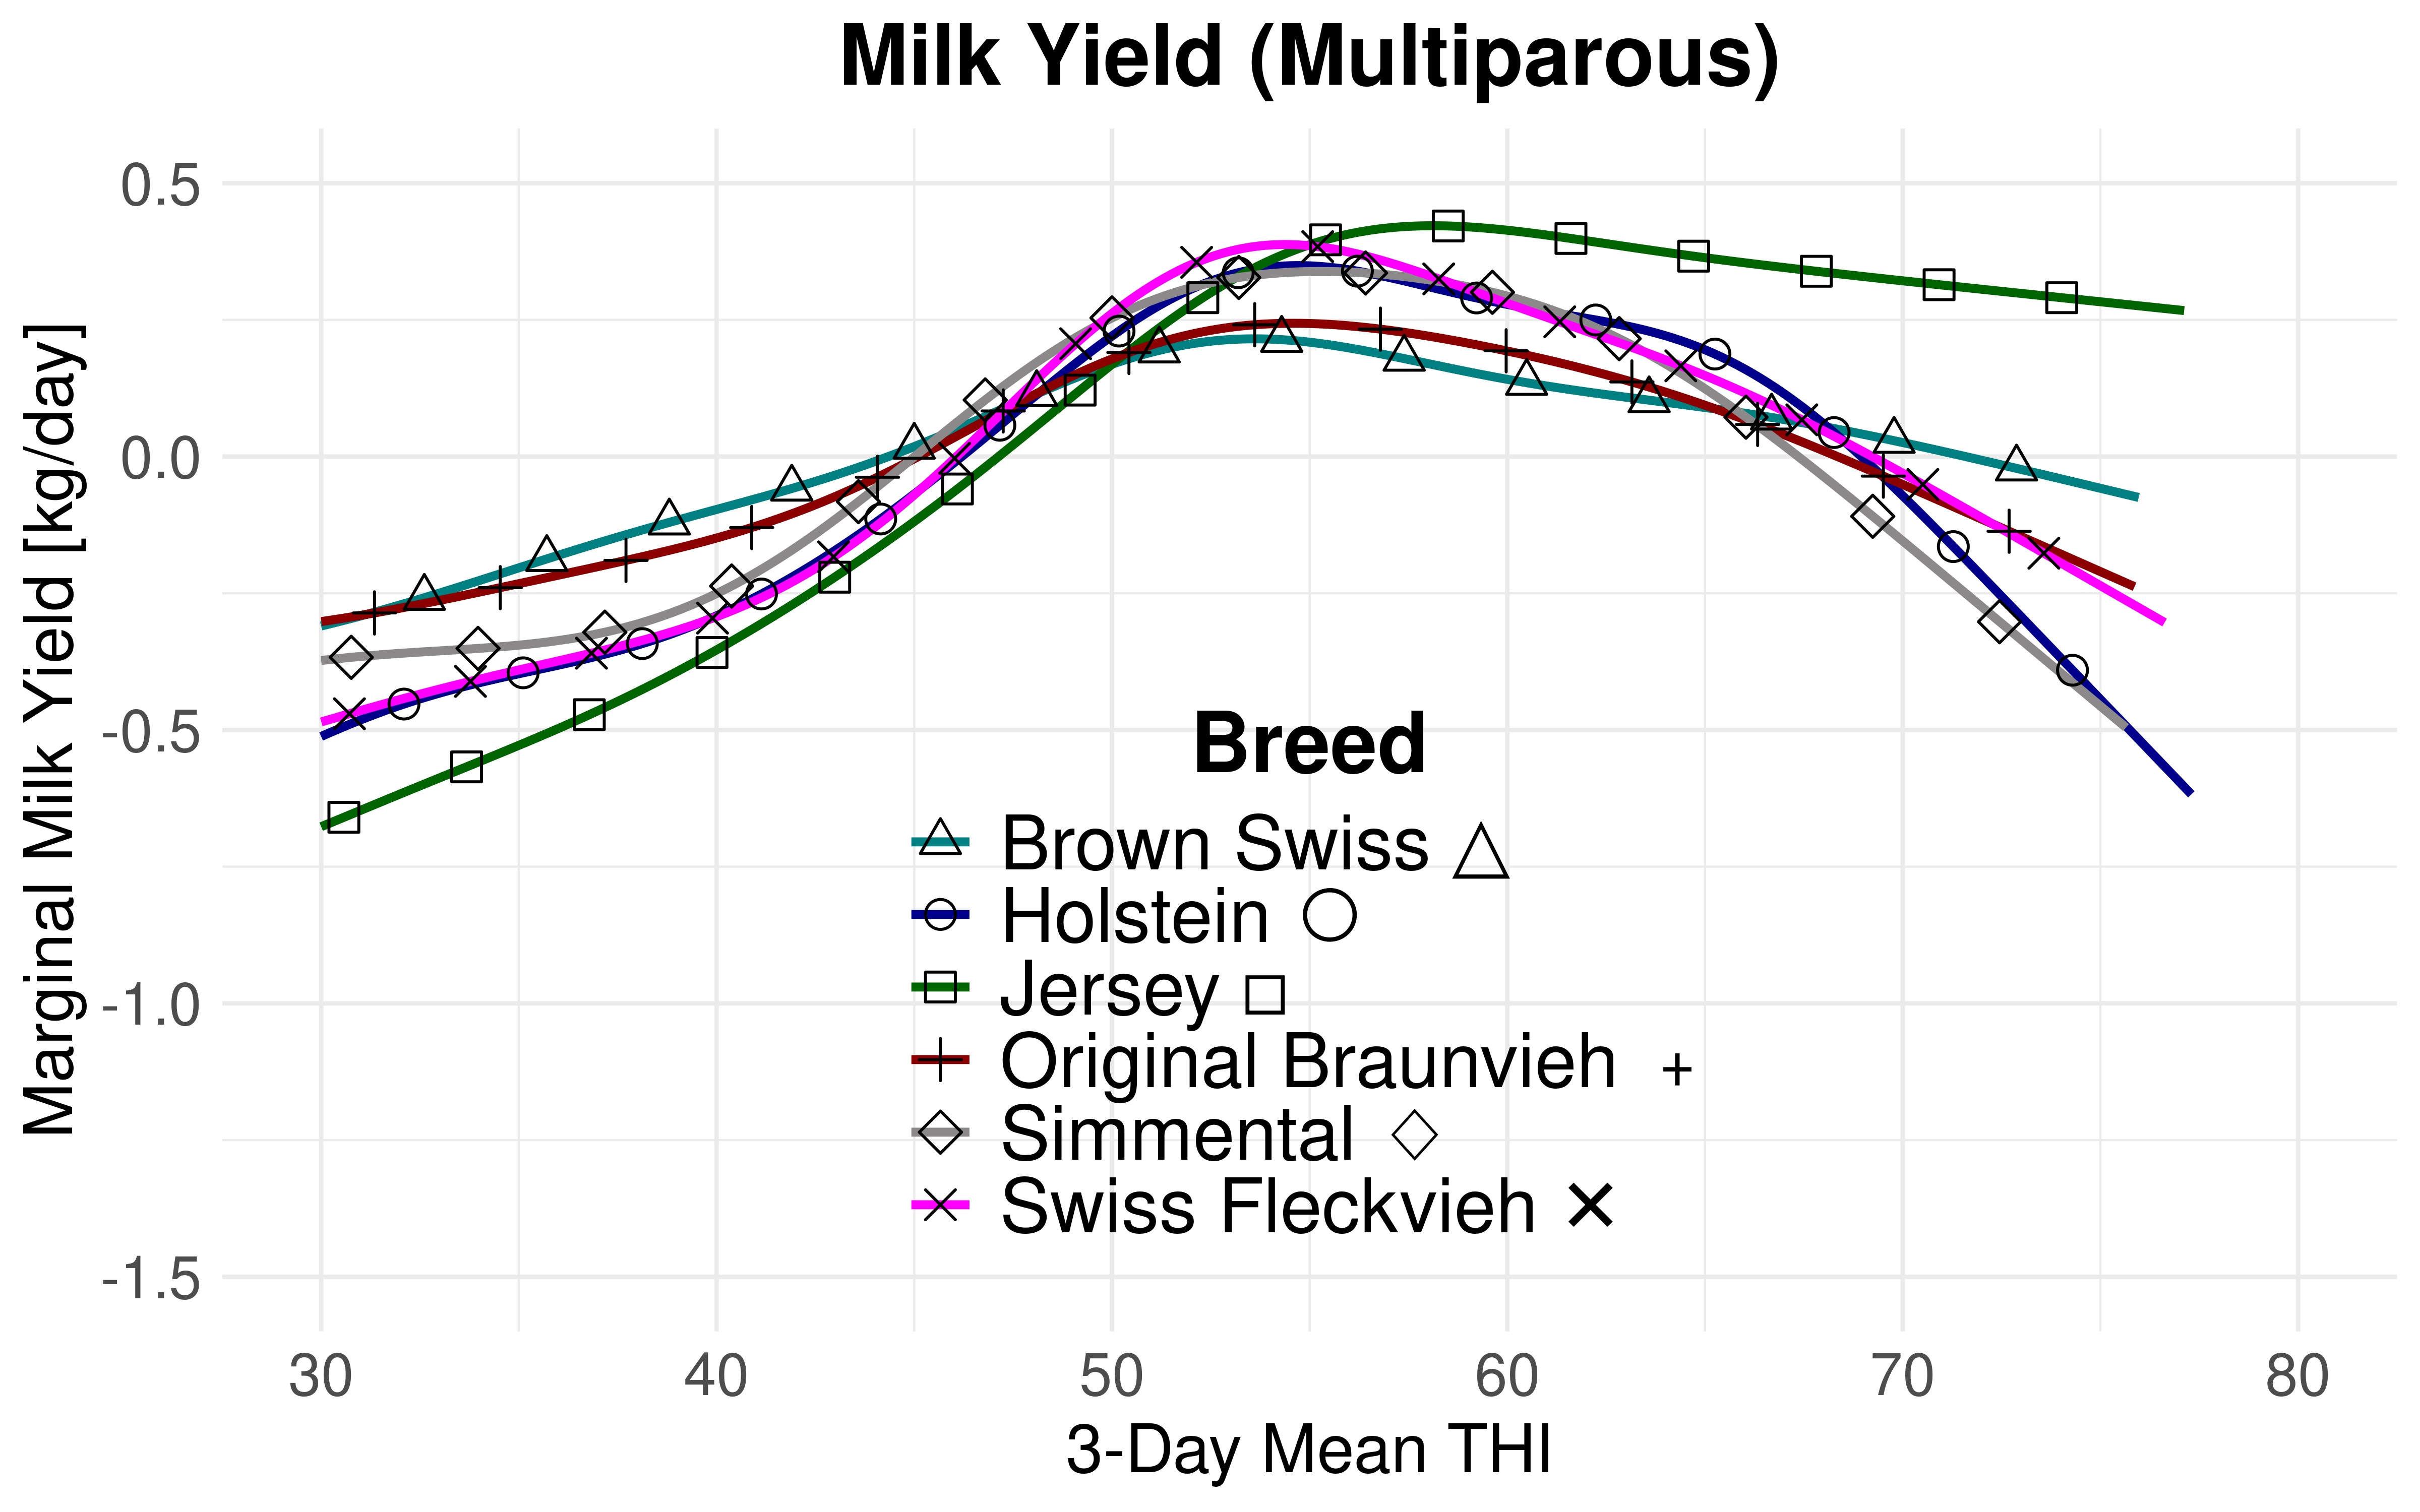
\includegraphics[width=\textwidth]{thesis/figures/results/milk_multiparous_overlapped.png}
        \caption{3-day mean marginal THI effect on milk yield multiparous Swiss dairy cows with data subsamples covering the full time period from 1982-2023.}
        \label{fig:milk_marginal_combined}
    \end{minipage}
    \hfill
    \begin{minipage}{0.49\textwidth}
        \centering
        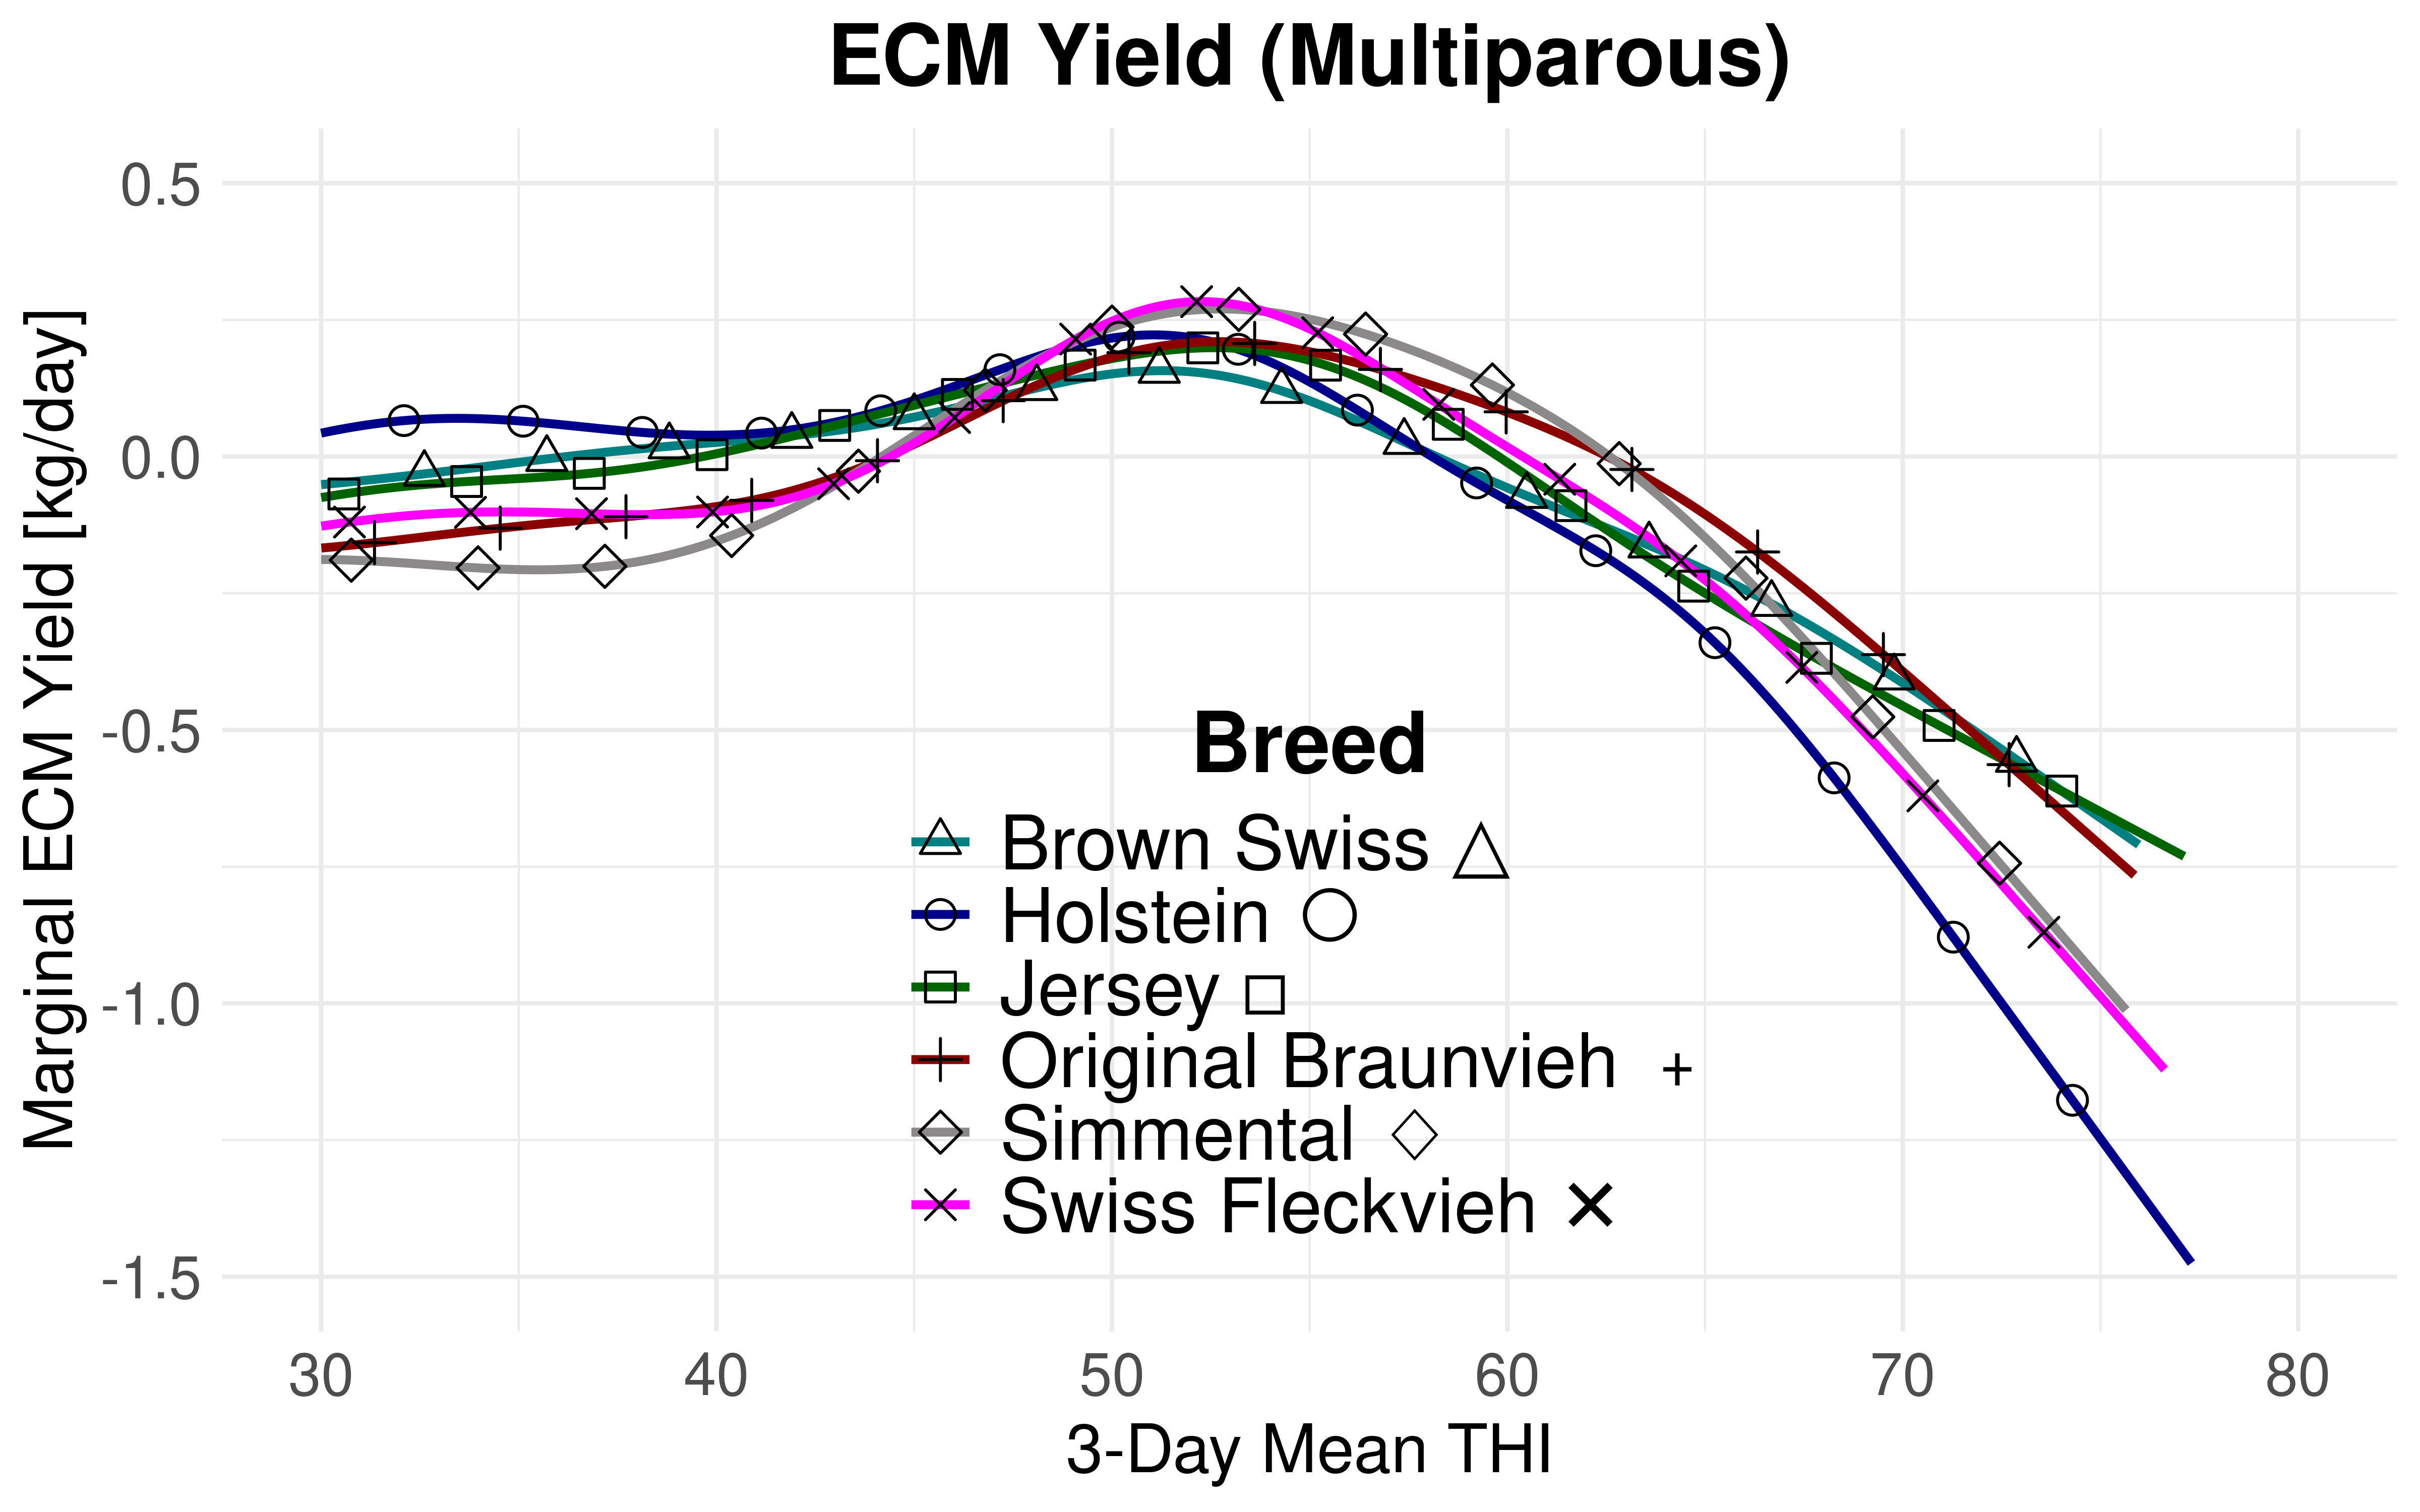
\includegraphics[width=\textwidth]{thesis/figures/results/ecm_multiparous_overlapped.png}
        \caption{3-day mean marginal THI effect on ECM yield multiparous Swiss dairy cows with data subsamples covering the full time period from 1982-2023.}
        \label{fig:ecm_marginal_combined}
    \end{minipage}
\end{figure}

The THI thresholds are lower for ECM yield compared to milk yield. Consequently, the milk component yields in relation to THI induce a leftward shift. Nonetheless, this shift does not remain uniform across all breeds. While the disparity between the lowest and highest THI turning points for milk yield is 4.56 for primiparous cows and 8.16 THI units for multiparous cows, the differences for ECM yield are notably smaller. Apparent benefits for certain breeds with respect to milk volume dissipate upon adjusting the milk volume for fat and protein yields. Figure~\ref{fig:milk_marginal_combined} and Figure~\ref{fig:ecm_marginal_combined} superpose the marginal effects of THI for each breed without confidence intervals to better illustrate this observation. The inverse relationship between THI and both fat and protein content is expected \citep{moore_how_2023}. \cite{vinet_estimation_2023} and \cite{hill_dairy_2015} have determined that declines in fat content in relation to THI manifest at an earlier stage or are stronger than protein declines. The specific individual contributions of protein and fat per breed to the observed shift and dissipation require further investigation.


\paragraph{Confidence Intervals}
The variability observed in the confidence intervals for each breed can be attributed to the employed subsampling strategy. The larger farms, the more samples per farm. Moreover, the available number of samples per farm also depends on the sampling strategy of the breeding associations. Table~\ref{table:milk_yield_subsample_stats_model_props} and Table~\ref{table:ecm_yield_subsample_stats_model_props} support this statement.  Consequently, our approach of incrementally incorporating farms into the dataset until a predetermined sample limit is reached results in a larger number of samples for these farms $t_s$. As a result, this approach contributes to diminished THI diversity, given that all samples gathered on a particular test-day at a given farm are associated with a single THI data point. This raises the question whether alternative subsampling methodologies at the farm level might need to be employed. Nonetheless, a careful interpretation of confidence intervals is necessary in this non-experimental study design and is further elaborated in Chapter~\ref{chap:conclusion}.

\paragraph{Split Period: Until 2010 - After 2010}
A striking difference emerges when splitting the data into two time periods: the THI turning points tend to be lower in the more recent data period from 2011 to 2023 compared to the period from 1982 to 2023. The Jersey breed poses an exception for ECM yield.

The average daily milk production is substantially higher today for all breeds relative to 13 years ago, attributed to successful breeding programs. The reduced THI turning points suggest that selective breeding has made dairy cows less tolerant to heat. The principal objectives of breeding are to enhance dairy performance with equivalent or relatively diminished input. Furthermore, long-term genetic selection exerts an influence on the metabolic system. The current selection strategies may prioritize enhancements in dairy performance without necessarily fostering heat resilience. As breeding continues to result in increased yields, offsetting heat-induced losses despite heightened heat exposure for dairy cows in Switzerland, this development potentially prompts more concerns regarding animal welfare rather than economic implications \citep{koenig_2023}. However, our results need further investigation with different cut-off years, multiple periods or different data subsampling strategies. Furthermore, shifts in THI turning points come along with changes in the loss rates. For example, simulations aggregating the daily effects with weather data over a long periods are necessary to further validate this negative change in heat-tolerance.
\chapter{Conclusion}\label{chap:conclusion}
We conclude this thesis by outlining our agronomic and computational contributions, and listing some limitations of the presented approach. We then outline some avenues for future research in this area.

\section{Contributions}

\paragraph{Agronomic Contributions} \quad \\
For the agronomic part, we determine performance-critical thresholds of THI on dairy performance for six dairy cow breeds within Switzerland. This includes the non-linear marginal effects of THI on milk and ECM yield for these breeds. The THI turning points begin as early as the high forties for primiparous cows and in the low fifties for multiparous cows, contingent upon the breed and performance variable. Prior research indicates a greater heat-resilience in primiparous cows relative to multiparous cows; however, our findings suggest the contrary. Next, we note varying non-linear marginal effects of THI on different breeds in terms of volumetric milk yield. Yet, these marginal effects align to very similar curves when the volume is adjusted with fat and protein to the ECM yield. Moreover, when the data is divided into two periods, 1982 to 2010 and 2011 to 2023, we observe that the THI turning point is generally lower in the more recent period. Furthermore, while not explicitly addressed in our research question, the incorporation of days in milk as a non-linear function enables the derivation of average lactation curves for each breed and facilitates the identification of lactation peaks utilizing the same methodology as a secondary outcome. These are not fully assessed in this work; however, they imply that lactation peaks may occur earlier than traditionally assumed.

To the best of our knowledge, even when subsampling, our investigation offers unprecedented granularity across geospatial and temporal dimensions. Furthermore, the data-driven smooth-term strategy utilizing GAMs isolates the THI effect while accounting for geospatial, locational, animal, and temporal factors with sparse yet extensive production data, greatly simplifying the methodology by requiring minimal initial assumptions about non-linearity of THI and the lactation curve. Generally, our research may be regarded as an advancement of \cite{bryant_quantifying_2007}, employing more recent computational and mathematical innovations, chiefly supported by \cite{wood_generalized_2017}.

\paragraph{Implications for Swiss Agriculture} \quad \\
Our results suggest that the thermoneutral zone for Swiss dairy cows is at a lower THI range than expected. When translated to a temporal context, this suggests that dairy cows are adversely affected by heat stress as early as March and continuing through to the late autumn months. These findings underscore the critical importance of well-chosen farm management strategies, including housing and feeding practices, to mitigate milk yield reductions and maintain animal welfare. Although further validation is necessary, the results for distinct periods suggest diminished heat tolerance in today's dairy cows. At present, increasing heat resilience is not a primary objective in breeding programs. However, given the anticipated rise in the frequency of hot days, such a breeding objective may be needed, depending on the progress in breeding for milk yield in the upcoming years.

\paragraph{Computational Contributions} \quad \\
For the computational part, arising from the challenges encountered with our sparse data structure as depicted in Figure~\ref{fig:dataset_structure_sparsity_dynamics} and the targeted estimation strategy delineated in Section~\ref{sec:estimation_strategy}, a bottleneck in the \textit{mgcv} GAM fitting routines is identified. As a remedy, we develop two prototype extensions for \textit{gamm4} in order to estimate Generalized Additive Mixed Models with a larger number of samples and random effect factor levels than previously achievable. \textit{gamm4b} represents a version with bug fixes and performance enhancements based on \textit{R}. \textit{gammJ} facilitates the estimation of GAMMs using a modified \textit{gamm4} along with a bridge to an adapted version of MixedModels.jl serving as the foundational estimation engine, complemented by a performance-optimized data covariance matrix decomposition for post-processing operations.

\section{Limitations}\label{sec:limitations}
\paragraph{High-Producing vs Low-Producing Cows}
The principal objective of our work is to determine the national average impact of the THI on dairy performance across different breeds. High-producing dairy cows are more susceptible to heat stress than their low-producing counterparts \citep{kadzere_heat_2002, de_rensis_seasonal_2015}. This particular aspect has not been incorporated into our current models and therefore, the consideration of production levels within our study remains incomplete. The unusually low peak THI values, alongside the residual patterns in diagnostic plots of the models, suggest that integrating this aspect could potentially enhance the model quality and provide a more lucid understanding of the peak THI values.

\paragraph{Single-Breed Models}
As elucidated in Section~\ref{sec:cholesky_scalable}, the principal limitation of \textit{gammJ} is not in the estimation of models that incorporate millions of samples and numerous random effect factor levels, but rather in the calculation of the data covariance matrix $\mathbf{V}$. This constraint hinders our capacity to estimate a multi-breed model as proposed in Equation~\ref{eq:multi_breed_model_extended}, as we foresee the requirement for at least several hundred thousand samples per breed. This conclusion is derived from model evaluations involving Jersey experiments as documented in Table~\ref{table:gamm4_performance}. While single-breed models allow for the estimation and visual examination of the THI effects on dairy performance across diverse breeds, they are insufficient for determining the statistical significance of the differences observed between these breeds. In a multi-breed model, wherein the effect of THI is interacted with the breed, an estimate of the statistical significance of each smooth is obtainable, and moreover, they can be visually compared safely as they originate from the same model. Furthermore, differences between smooth terms can be computationally discerned \citep{gavin2017difference, gavin2017differenceII}. When comparing smooth terms of distinct single-breed models, a robust comparison is feasible only if one can substantiate that all terms in a corresponding multi-breed model are interacted by breed. The justification for such an interaction for all model terms is partially addressed in Section~\ref{sec:multi_breed_model}, but the general question is still open.

\paragraph{Subsampling}
Section~\ref{sec:model_overview} and the corresponding results demonstrate the influence of farm and sampling structure on the THI diversity within our subsamples. This influence is further reflected in the model's confidence intervals. The central argument underpinning the subsampling strategy outlined in Chapter~\ref{chap:results} is the implicit maintenance of farm structure within the model. Consequently, given the imposed limitation on the maximum number of samples due to computational constraints, it becomes pertinent to explore whether the current subsampling strategy remains suitable, since in scenarios the number of farms merely amounts to several hundred. For example, considerations may be made towards relaxing the assumption regarding farm structure and update the sampling strategy accordingly.

\paragraph{Limited Interpretability of P-Values and Spatial Autocorrelation} The field-derived data is acquired from operational agricultural environments, with the objective of overseeing breeding advancements and facilitating long-term analytics. This data is not derived from an experimental design, as elaborated in Section~\ref{sec:data}. Data collection includes repeated measurements for each animal and farm. On designated sampling days, data from all animals within a farm is collected concurrently. The geospatial distribution of farms introduces regional dynamics and topological diversity, which are further influenced by meteorological conditions. Therefore, the samples are not independent and identically distributed. This is why we use a mixed model. We partially control for group, spatial and temporal dynamics with animal $\alpha$, farm $\phi$ and spatio-temporal $\iota$ random effect terms in our models. Nonetheless, the issue of autocorrelation is not addressed in the error terms $\epsilon$, which are under \textit{iid} assumption in a mixed model framework, nor is it considered within the model weights because both \textit{lme4} and \textit{MixedModels.jl} lack implementation of such structures. Consequently, although a larger sample size results in significant p-values, these p-values lack interpretative validity. The same applies to confidence intervals. Nevertheless, the reliability of the estimated fixed effect coefficients and smooth terms remains unaffected, as they are derived from a substantial dataset comprising hundreds of thousands of samples. However, it is imperative to exercise utmost caution when interpreting confidence intervals and conducting hypothesis testing.

\paragraph{Farm Location as Fixed Effects} Both, random and fixed effects, are applied to account for unobserved heterogeneity. In this context, \citet[Chapter 10]{woolridge_2010} examines the assumptions underlying both fixed and random effects models. The assumption associated with random effects suggests that unobserved individual heterogeneity remains uncorrelated with the covariates. In contrast, the fixed effects assumption allows for the possibility that these individual-specific effects may be correlated with the explanatory variables. Drawing from this econometric perspective, it can be asserted that the farm location random effect $\phi$ demonstrates a certain degree of correlation with the THI smooth function f(THI), thereby contravening the assumption of random effects. Consequently, it may be advocated that the unobserved heterogeneity associated with farm location should be represented through fixed effects. Notably, in \cite{bryant_quantifying_2007}, individual herds are modeled as fixed effects. A qualitative argument posits that constraining the individual farm coefficients by modeling them as random intercepts could be overly restrictive. The variability in farming practices and conditions may not be adequately captured by a normal distribution of these coefficients. Conversely, an argument in favor of treating individual farms as random intercepts arises from the limited subset of farms utilized in our subsamples. Despite this, farm coefficients are modeled as random effects in all our experiments for a practical reason: Most mixed model libraries do not implement the fixed effect matrix as sparse matrices, which would be a requirement given the number of farms in our dataset. \textit{MixedModels.jl} does indeed provide support for sparse fixed effect matrices. However, due to time constraints, models where individual farms are treated as fixed effect coefficients have not been tested. Nevertheless, this debate surrounding farms as fixed effects requires more attention. 

\paragraph{Additional Weather Variables as Control}
Our models do not control for additional weather variables such as radiation, sunshine duration, or precipitation. As indicated in Chapter~\ref{chap:background}, these factors similarly influence a dairy cow's heat management. Consequently, the effect of THI not be completely isolated. Therefore, it could be advantageous to conduct experiments that control for these variables, notwithstanding the possibility that they might confound with temperature and relative humidity. An example study which applies this methodology for test-day milk samples is \cite{ahmed_temperature_2022}.


\section{Future Research}
Finally, we outline seven opportunities for extension of this work into multiple directions.

\vspace*{\baselineskip}
First, the preceding section underscores the necessity to conduct further experimentation in model selection and subsampling strategies. This involves a meticulous examination of whether single breed models are adequate to facilitate a valid comparison among breeds.

\vspace*{\baselineskip}
Second, it is essential to address the distinction between high- and low-producing cows. In this context, data splits as straightforward as milk yield above $\mu + \frac{\sigma}{2}$ for high-producing and below $\mu - \frac{\sigma}{2}$ for low-producing cows could serve as an initial framework.

\vspace*{\baselineskip}
Third, other dimensions of model selection merit attention, including the decision between random effects and fixed effects for farm location, additional controls for weather, as well as considerations of autocorrelation. Generally, model selection involving mixed models requires the use of maximum likelihood estimation \textit{ML} instead of restricted maximum likelihood \textit{REML} to ensure their comparability with model selection criteria such as the Akaike Information Criterion \citep{bozdogan_model_1987}. To date, our extension from Section~\ref{sec:gamm4_modifications} has only been tested with \textit{REML}, as a comprehensive model selection process has not yet been pursued. Our parameter investigation has prioritized the appropriate determination of degrees of freedom for the smooth terms, for which we used estimated degrees of freedom from \textit{mgcv} as a selection criterion. In addressing autocorrelation aspects with GAMMs, \textit{spatial+} by \cite{dupont_spatial_2020} might be considered. Additionally, incorporating spatial coordinates such as longitude and latitude, as well as the day of the year for temporal aspects, as smooth terms could potentially address autocorrelation concerns. Alternatively, \cite{bolker_glmmFAQ} posits that the integration of spatial correlation functions into \textit{lme4} is not an immediate priority, but should be reportedly straightforward to implement in the context of linear mixed models. It is reasonable to infer that this assertion extends to the \textit{MixedModels.jl} library as well.

\vspace*{\baselineskip}
Fourth, the effect of additional dairy performance variables from THI could be investigated, such as lactose and somatic cell count. Both of these are relevant for quality and health aspects. Moreover, the component yields such as fat and protein could be analyzed individually, in addition to the energy-corrected milk (ECM) yield to better understand which and how much they contribute to the observed phenomenon of aligned ECM curves for individual breeds.

\vspace*{\baselineskip}
Fifth, our models do not include interactions between THI and days in milk. Given that GAMs can incorporate multi-dimensional smooth terms, exploring a two-dimensional smooth function $f(THI, DIM)$ could enhance both the interpretability and representativeness of the modelling.

\vspace*{\baselineskip}
Sixth, the models employed in this study do not include the weather exposure experienced by dairy cows prior to parturition. Additionally, they do not consider breeding ancestry or supplementary physiological data available. The data furnished by the three associations, in conjunction with the available meteorological data, would facilitate such expansions.

\vspace*{\baselineskip}
Seventh, the library \textit{mgcv} developed by Simon Wood demonstrates high computational efficiency for generalized additive models (GAMs) when applied to datasets characterized by a large number of samples but limited in the diversity of factor levels. The methodologies we have formulated in Section~\ref{sec:gamm4_modifications} partially bridge this gap. Nevertheless, further empirical validation and optimizations are necessary to make these innovations ready for broader use in academic and industrial applications.
%% ----------------------------------------------------------------
\thesisbib

\thesisappendix
%\thesisbib
\begin{appendices}
	\newpage
\chapter{THI Table}
The following Figure~\ref{fig:thi_table} is a THI table with an extended temperature range compared to the commonly available THI tables. We use the THI specification from \cite{nrc_1971}. The table facilitates the interpretation of our findings in Chapter~\ref{chap:results}.
\begin{figure}[H]
    \centering
    \includegraphics[width=\textwidth]{thesis/figures/THI_NRC_extended.pdf}
    \caption[]{THI Table with an extended temperature.}
    \label{fig:thi_table}
\end{figure}
\newpage


\chapter{Source Code}\label{appendix:source_code}
\begin{center}
The repository of this thesis is: \\
\href{https://github.com/an-ethz/heat4milk-report}{https://github.com/an-ethz/heat4milk-report}
\end{center}
\section*{Notebooks}
\begin{itemize}
    \item \url{heat4milk-report/notebooks/preprocessing} Data Preprocessing (Section~\ref{sec:data})
    \item \url{heat4milk-report/notebooks/models/gamm} Single Breed Models (Chapter~\ref{chap:results})
    \item \url{heat4milk-report/notebooks/models/figures} Plotting Templates (Chapter~\ref{chap:results})
    \item \url{heat4milk-report/notebooks/models/fixed_effect_econometrics} (Section~\ref{sec:discussion})
\end{itemize}

\section*{gamm4b}
\begin{itemize}
    \item \url{heat4milk-report/src/gamm4b/gamm4b_example.ipynb} Example notebook with dissected \textit{gamm4} and proposed modifications (Section\ref{sec:gamm4b})
\end{itemize}

\section*{gammJ}
\begin{itemize}
    \item \href{https://github.com/an-ethz/MixedModels.jl}{https://github.com/an-ethz/MixedModels.jl} Modified \textit{MixedModels.jl} (Section~\ref{sec:julia_modifications})
    \item \url{heat4milk-report/src/gammJ/gammJ_v9_example.ipynb} Example notebook with dissected \textit{gamm4} and modified MixedModels.jl as fitting engine (Section~\ref{sec:gammJ}). This is the gammJ entrypoint.
    \item \url{heat4milk-report/src/gammJ/trainGAM.jl} Model estimation called by \textit{gammJ} (Equation~\ref{eq:gamm_glmm})
    \item \url{heat4milk-report/src/gammJ/postprocessGAM.jl} Julia Post-processing operations called by \textit{gammJ} (Section~\ref{sec:cholesky_scalable})
\end{itemize}


\chapter{Split Period: Until 2010 - After 2010}\label{appendix:split_period}

The following pages provide the summarizing figures with the THI curves for the split-period models.
\newpage
\begin{landscape}
    \thispagestyle{empty}
    \section{Milk Yield}
    \begin{figure}[ht]
        \centering
        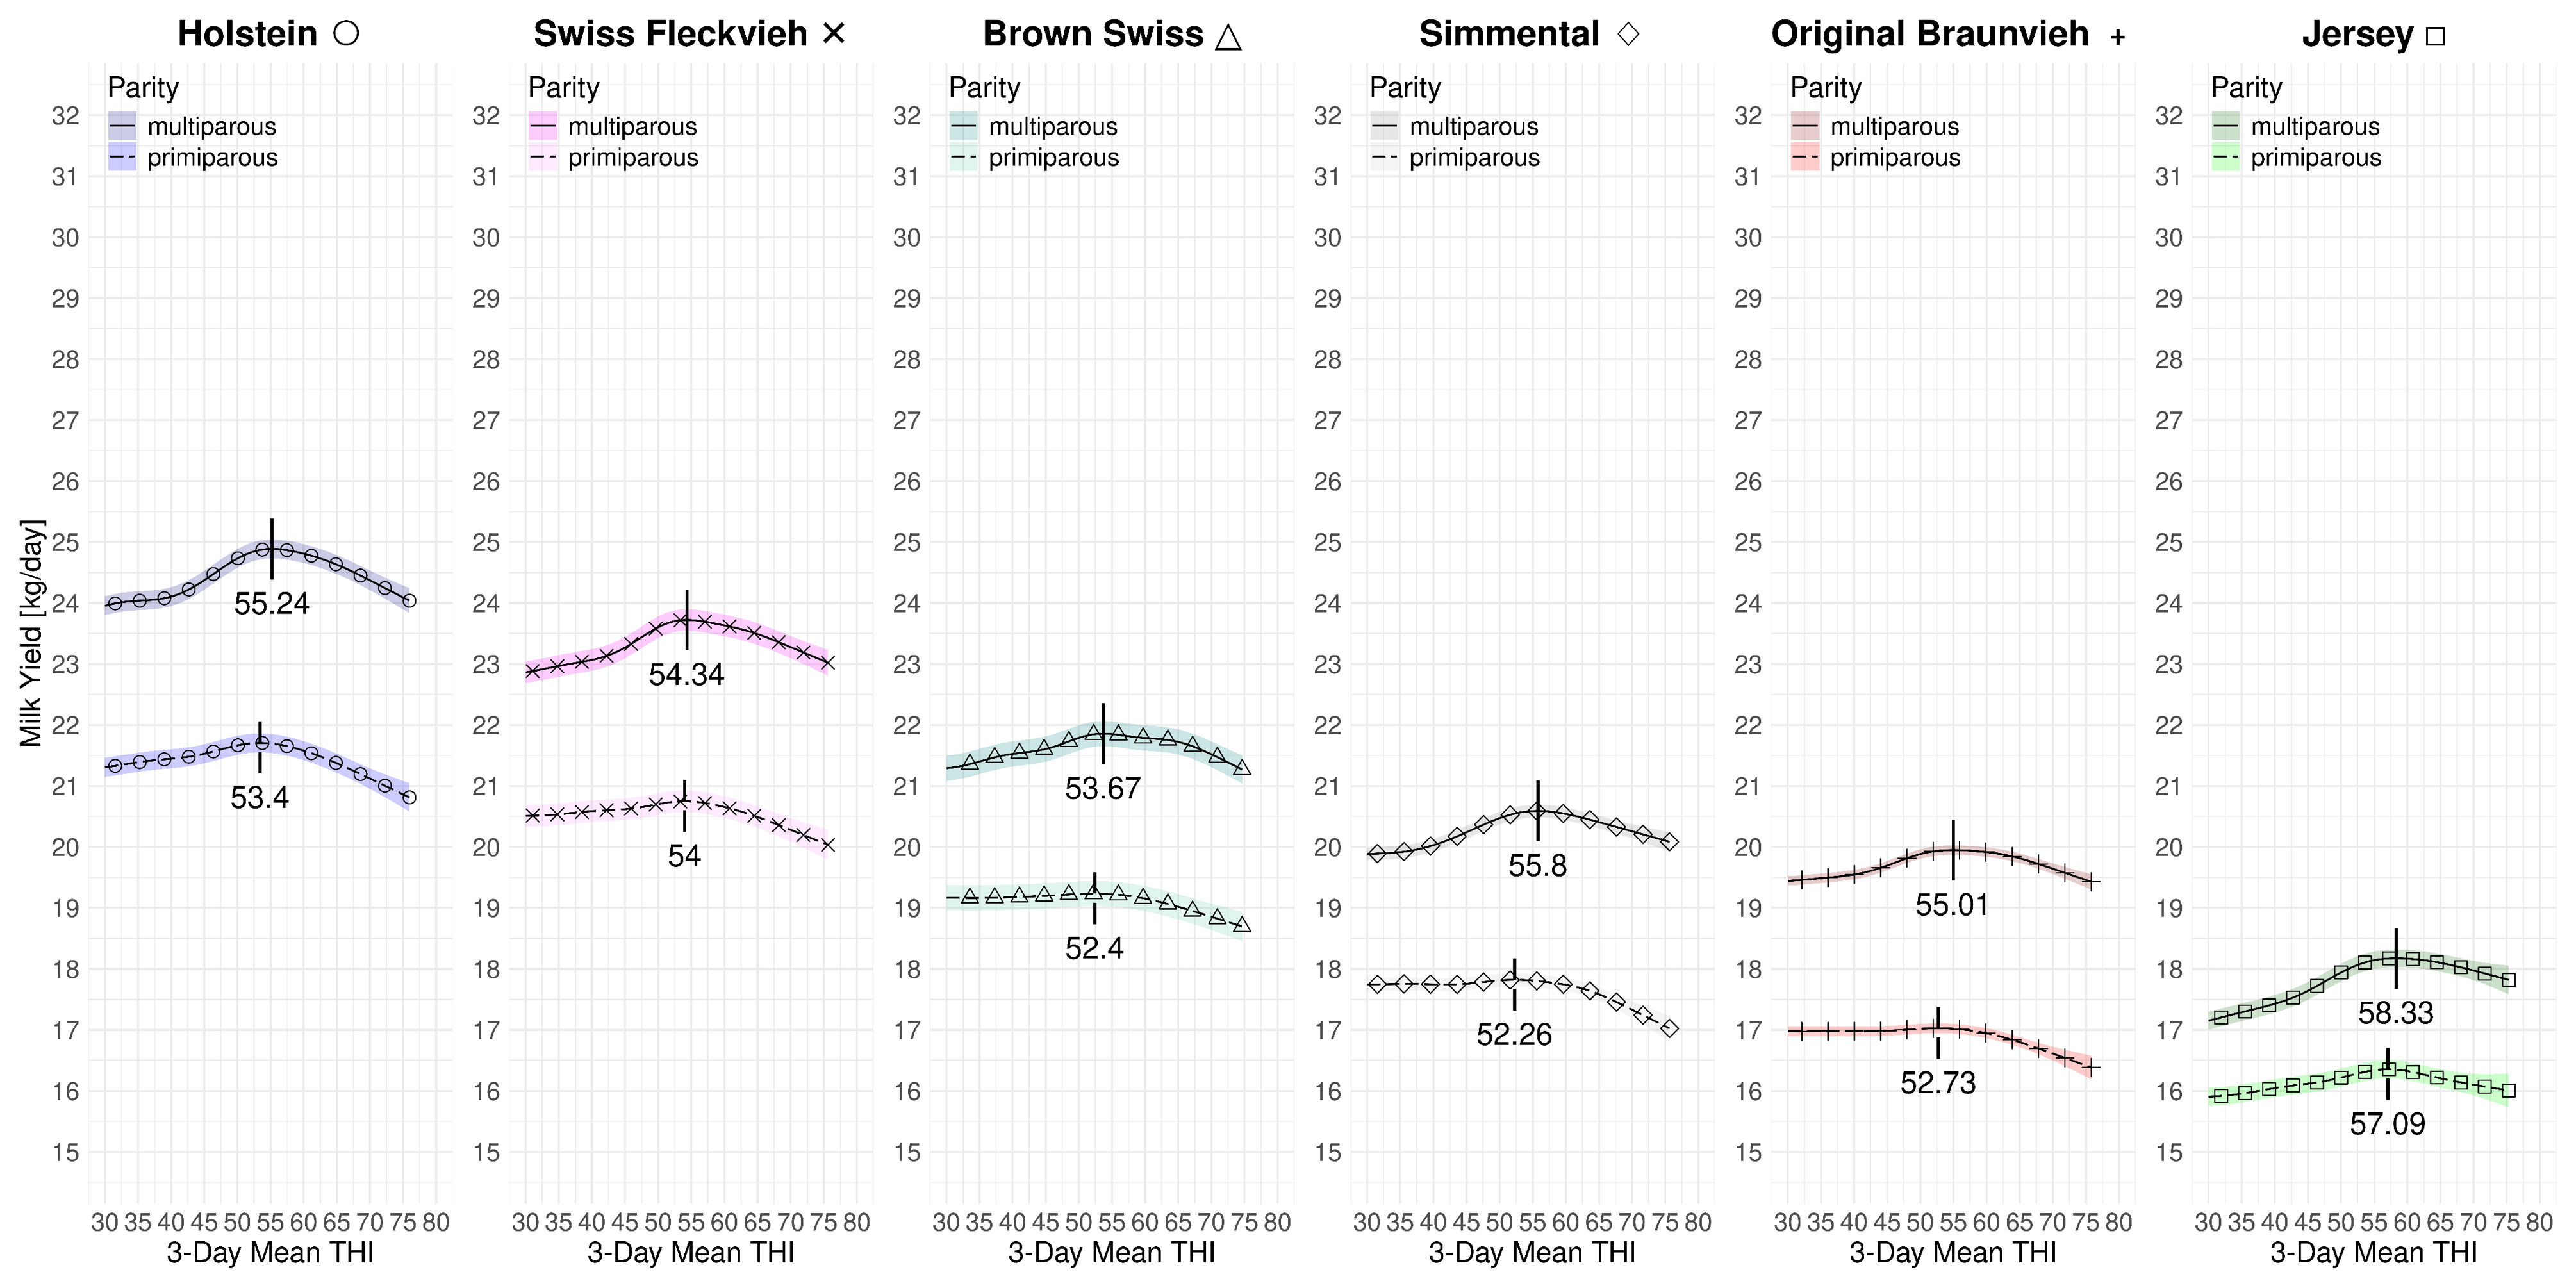
\includegraphics[width=0.85\paperheight]{thesis/figures/results/milk_yield_before_2010.png}
        \caption[]{3-day mean THI effect on milk yield for primi- and multiparous Swiss dairy cows at 2010 levels with data subsamples covering the full time period from 1982-2010.}
        \label{fig:results_milk_yield_before_2010}
    \end{figure}
    
    \begin{textblock*}{2cm}(20cm, \dimexpr\paperheight/2)
    \rotatebox{90}{\thepage}
    \end{textblock*}
\end{landscape}

\newpage
\begin{landscape}
    \thispagestyle{empty}
    \begin{figure}[ht]
        \centering
        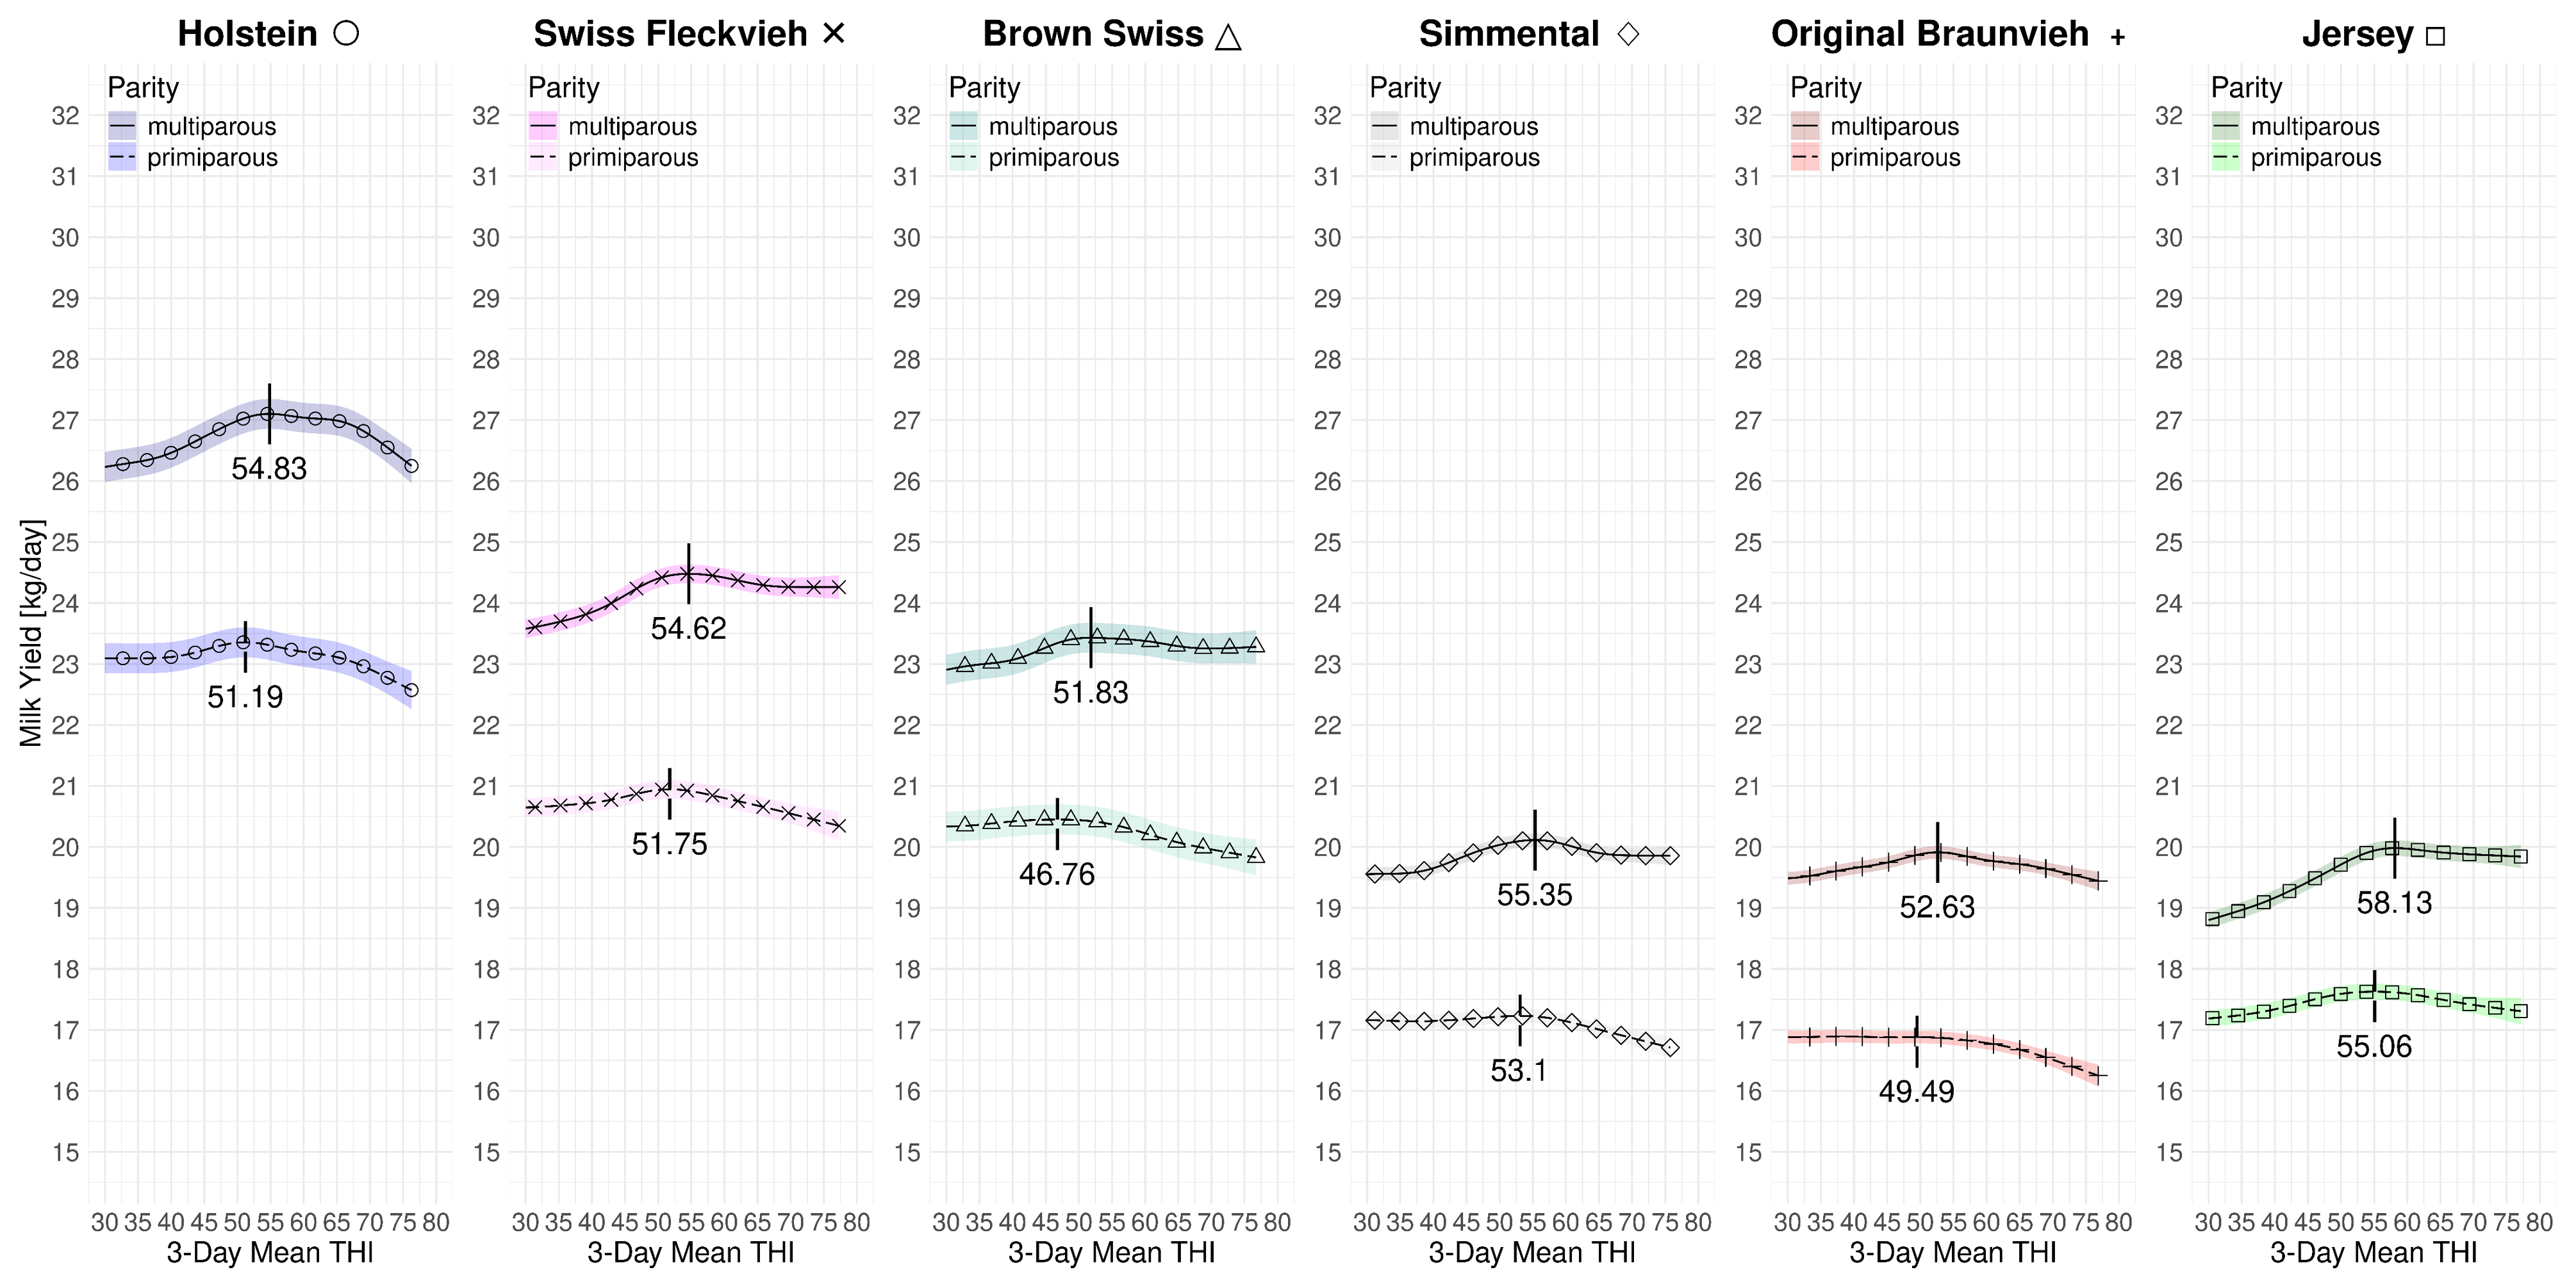
\includegraphics[width=0.85\paperheight]{thesis/figures/results/milk_yield_after_2010.png}
        \caption[]{3-day mean THI effect on milk yield for primi- and multiparous Swiss dairy cows at 2023 levels with data subsamples covering the full time period from 2011-2023}
        \label{fig:results_milk_yield_after_2010}
    \end{figure}
    
    \begin{textblock*}{2cm}(20cm, \dimexpr\paperheight/2)
    \rotatebox{90}{\thepage}
    \end{textblock*}
\end{landscape}


\newpage
\begin{landscape}
    \thispagestyle{empty}
    \section{ECM Yield}
    \begin{figure}[H]
        \centering
        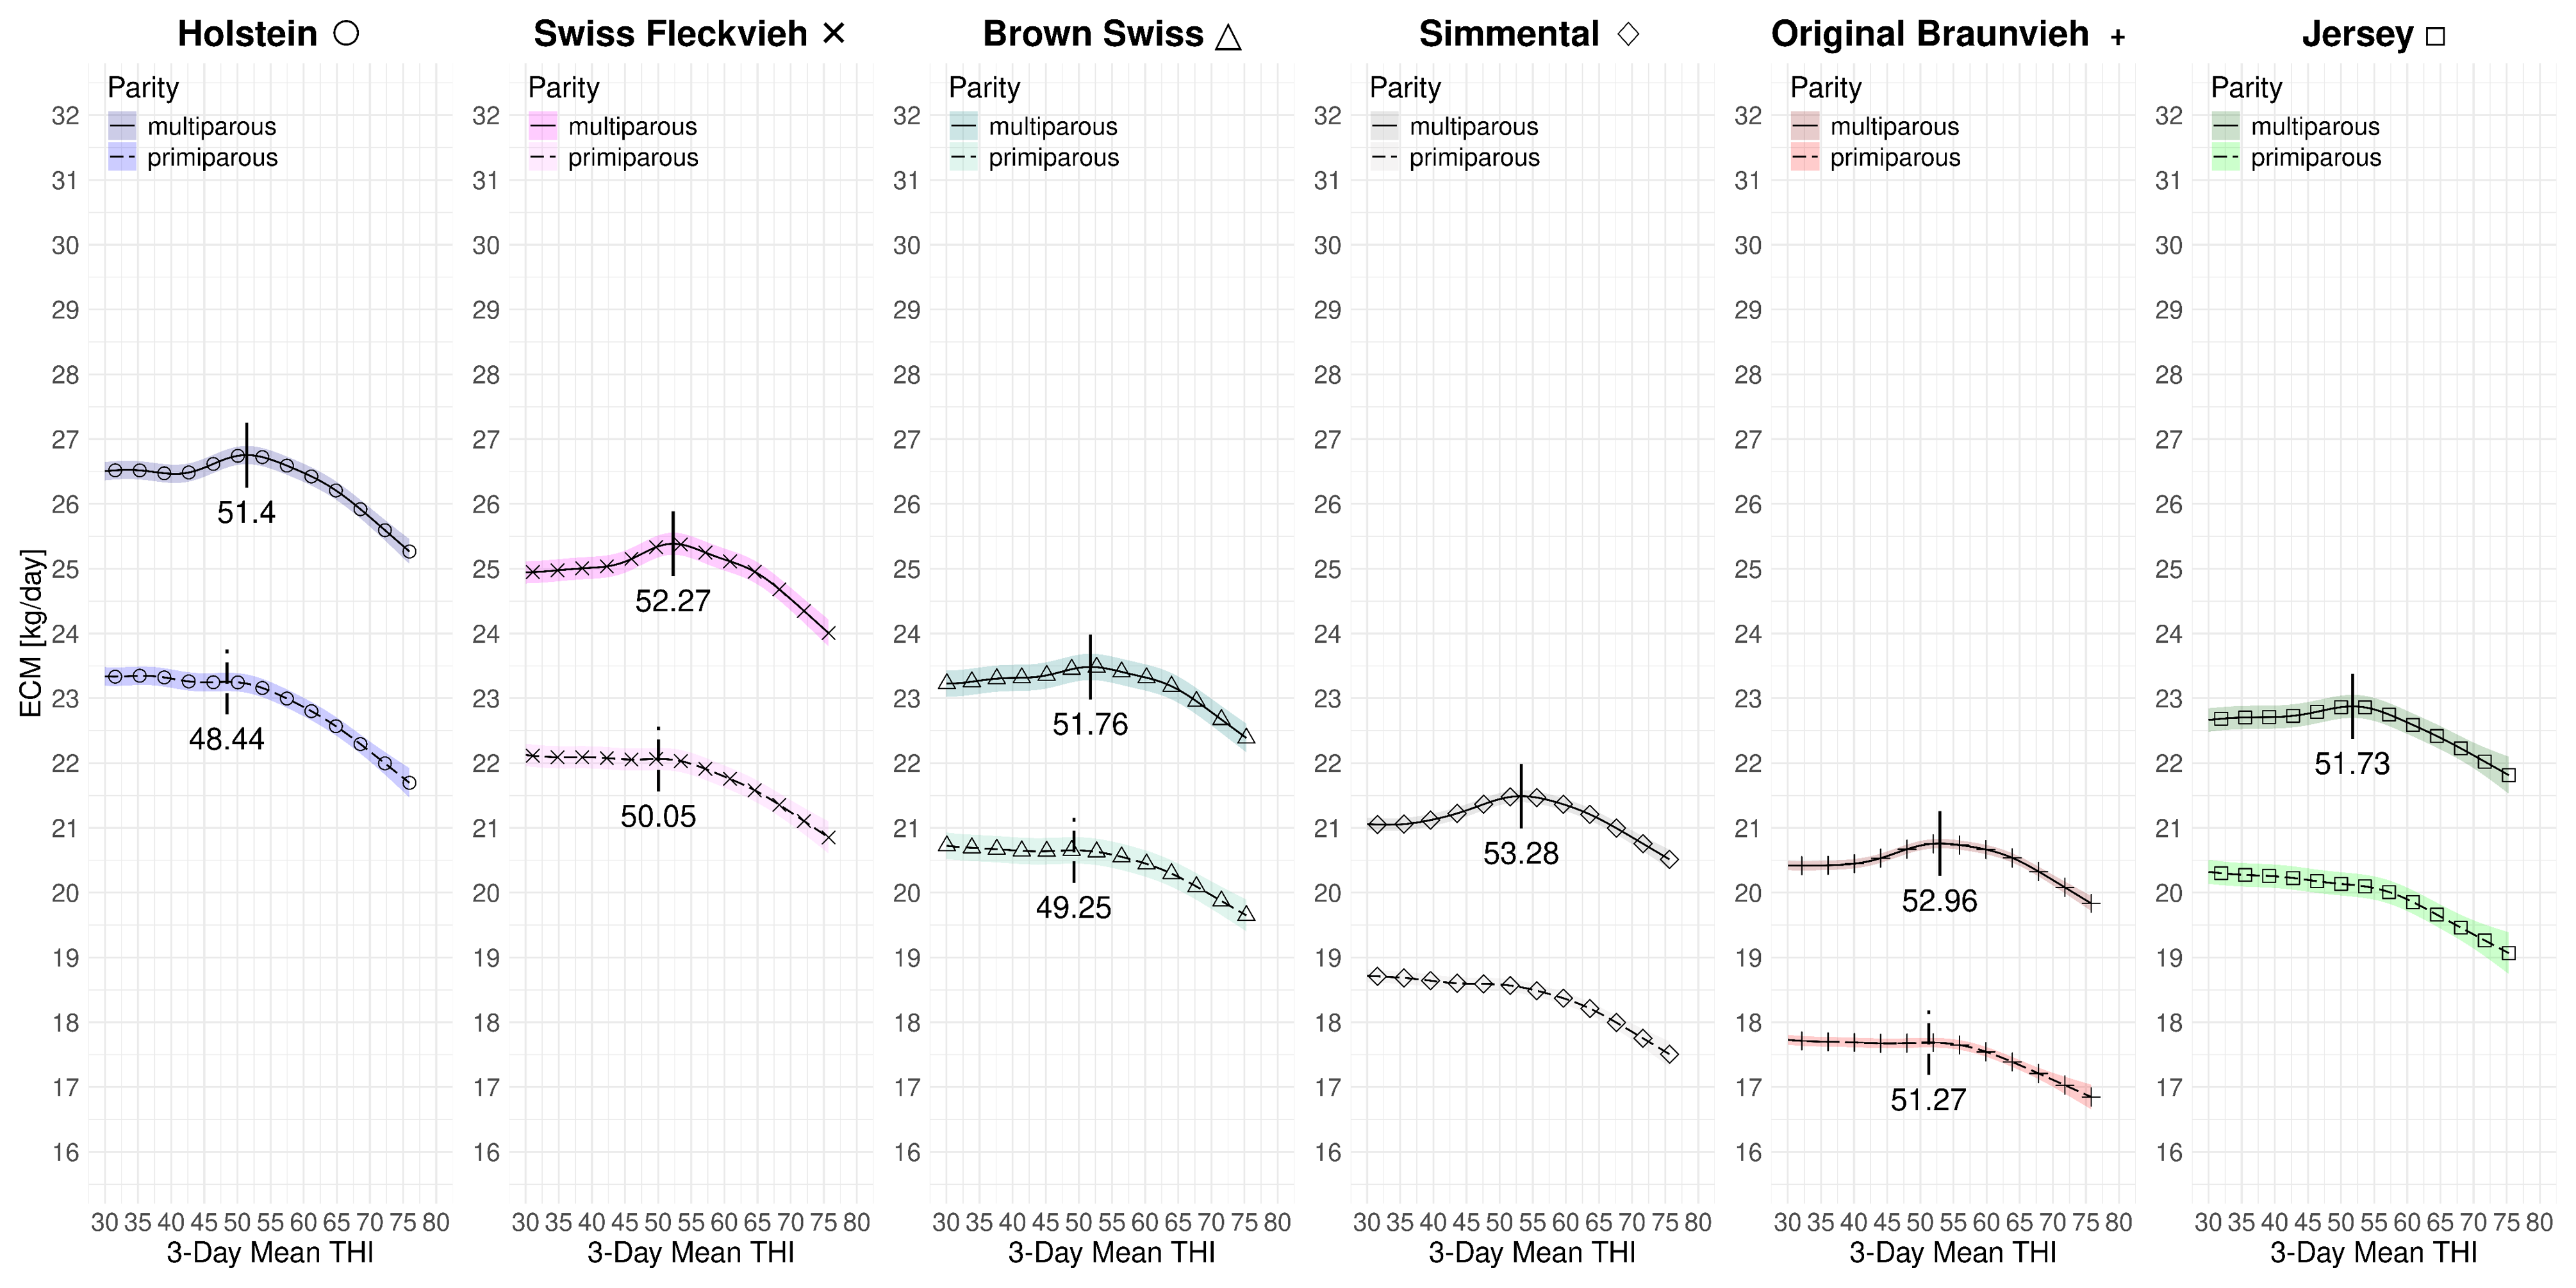
\includegraphics[width=0.85\paperheight]{thesis/figures/results/ecm_yield_before_2010.png}
        \caption[]{3-day mean THI effect on ECM yield for primi- and multiparous Swiss dairy cows at 2010 levels with data subsamples covering the full time period from 1982-2010.}
        \label{fig:results_ecm_yield_before_2010}
    \end{figure}
    
    \begin{textblock*}{2cm}(20cm, \dimexpr\paperheight/2)
    \rotatebox{90}{\thepage}
    \end{textblock*}
\end{landscape}
\newpage

\begin{landscape}
    \thispagestyle{empty}
    \begin{figure}[ht]
        \centering
        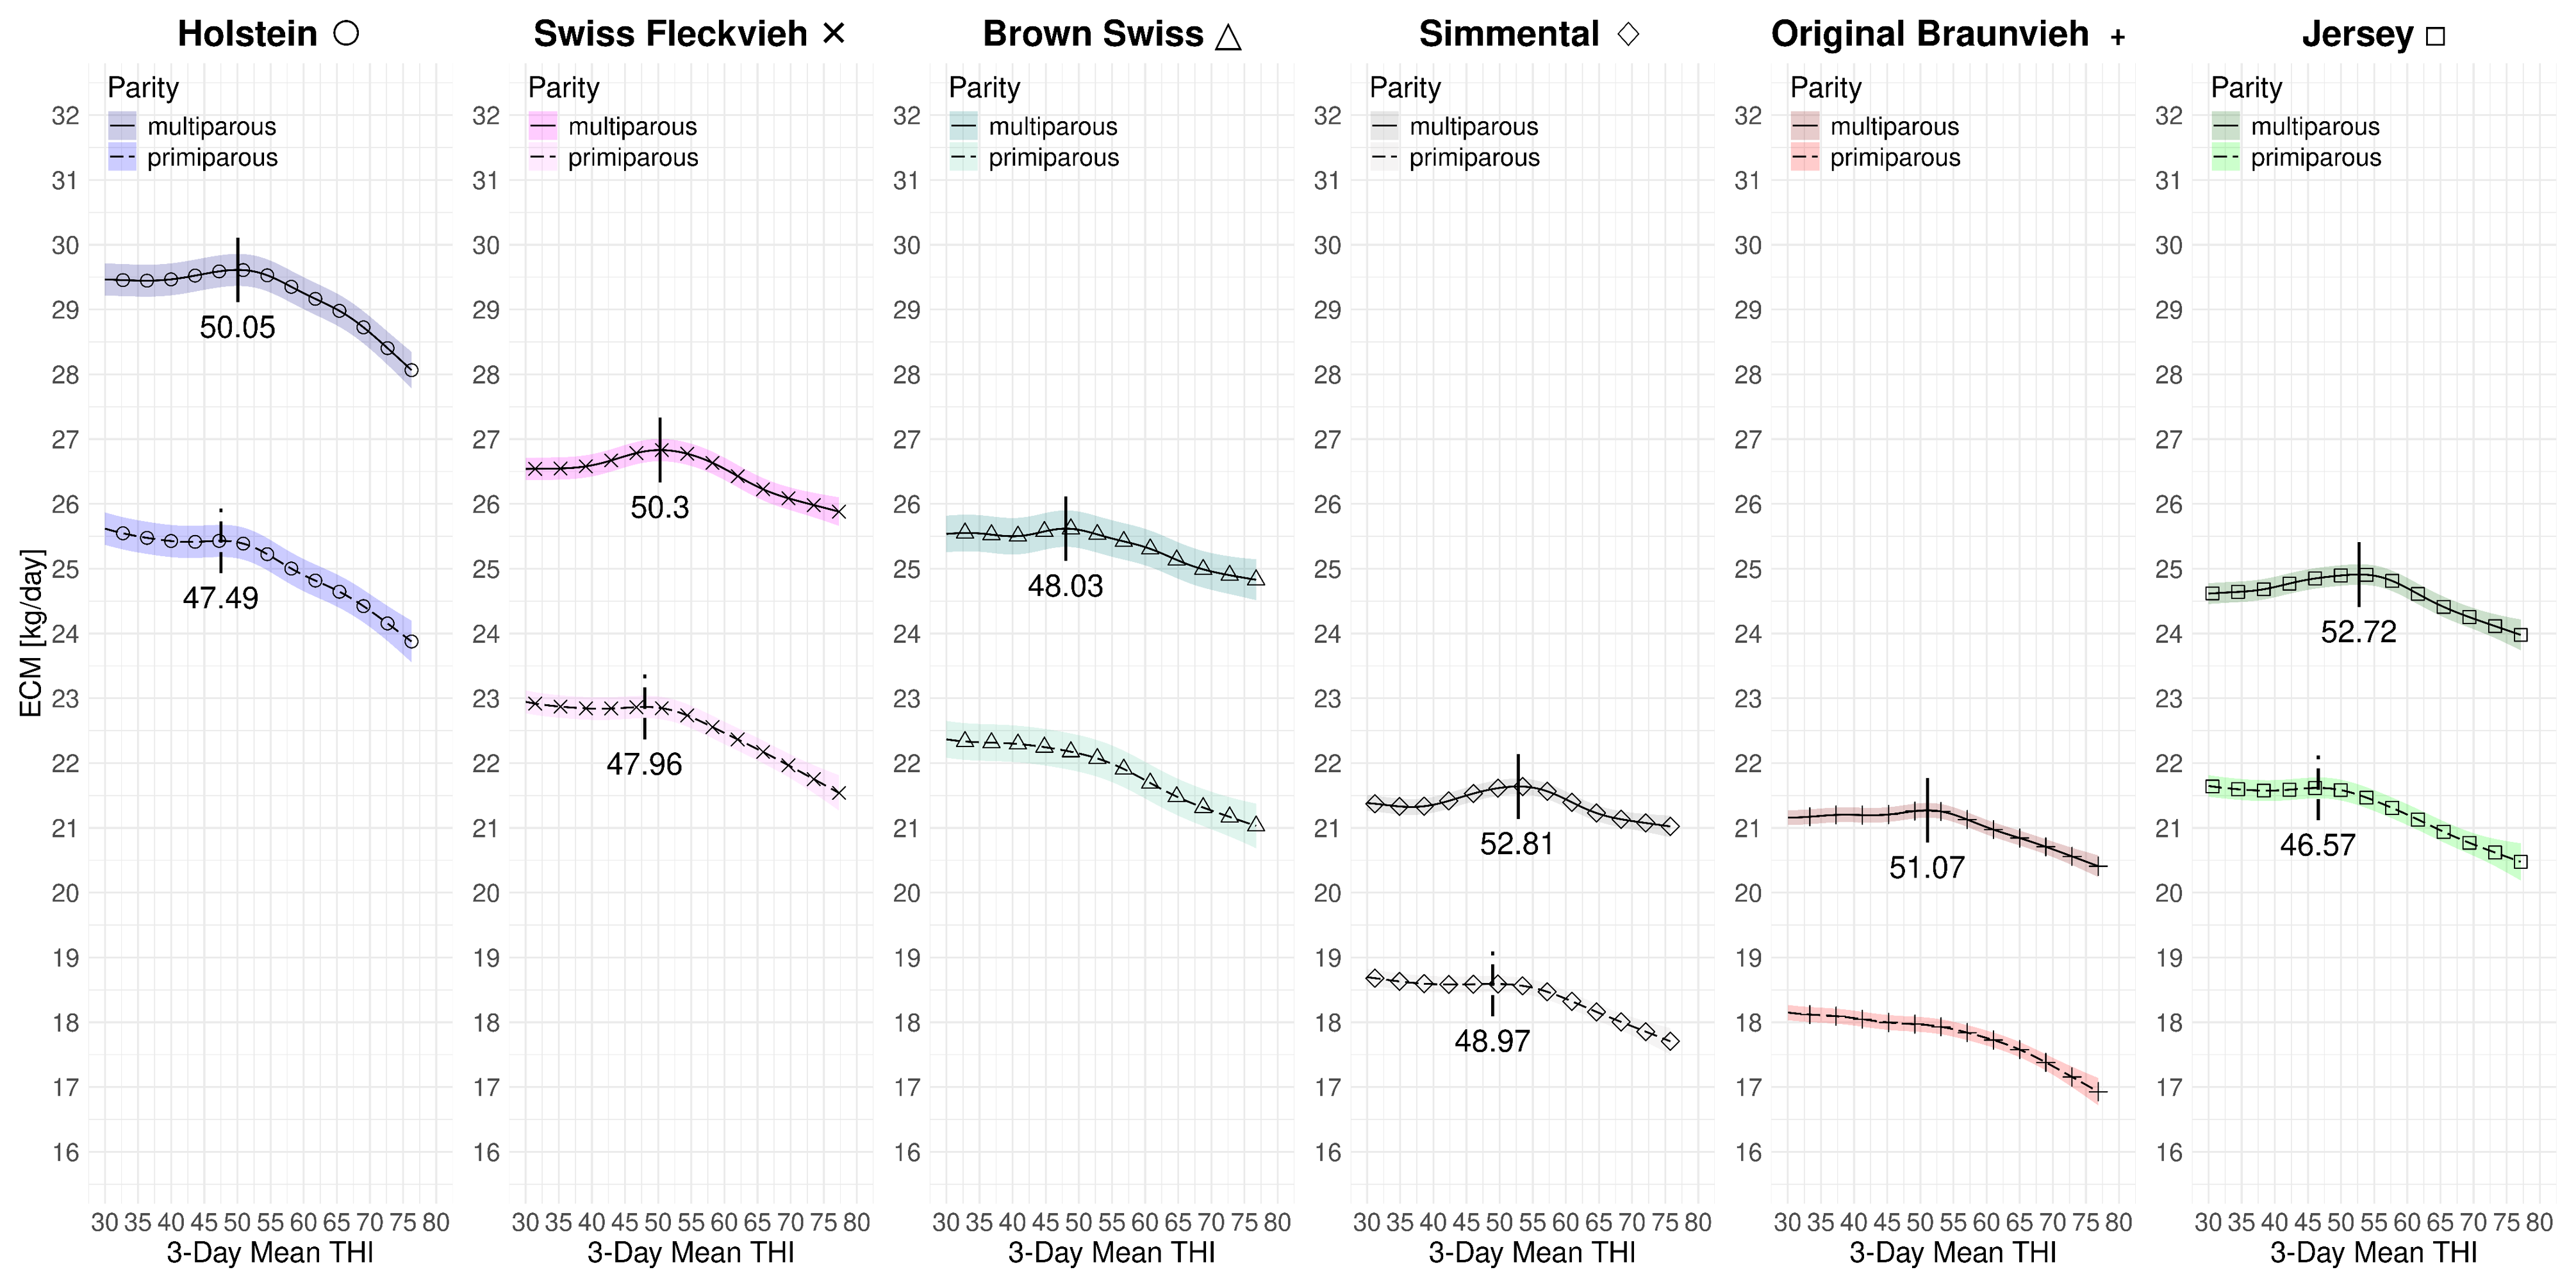
\includegraphics[width=0.85\paperheight]{thesis/figures/results/ecm_yield_after_2010.png}
        \caption[]{3-day mean THI effect on ECM yield for primi- and multiparous Swiss dairy cows at 2023 levels with data subsamples covering the full time period from 2011-2023.}
        \label{fig:results_ecm_yield_after_2010}
    \end{figure}
    
    \begin{textblock*}{2cm}(20cm, \dimexpr\paperheight/2)
    \rotatebox{90}{\thepage}
    \end{textblock*}
\end{landscape}


\chapter{Models}\label{appendix:models}

\newpage
\section{Holstein: Milk Yield}
\subsection{Full Period: 1985-2023}\label{model:ho_milk_full}
\paragraph{Model Summary} \quad \\

    \begin{table}[H]
    \centering
    \begin{tabular}{lrrrr}
    \textbf{A. parametric coefficients} & Estimate & Std. Error & t-value & p-value \\ 
       \hline
       \hline
  (Intercept) & 17.8235 & 0.6916 & 25.7716 & $<$ 0.0001 \\ 
  parityprimiparous & -3.4189 & 0.0129 & -264.1612 & $<$ 0.0001 \\ 
  year1986 & 0.3265 & 0.3478 & 0.9389 & 0.3478 \\ 
  year1987 & 0.1965 & 0.5377 & 0.3654 & 0.7148 \\ 
  year1988 & 0.0287 & 0.6610 & 0.0435 & 0.9653 \\ 
  year1989 & 0.5588 & 0.8363 & 0.6682 & 0.5040 \\ 
  year1990 & 0.8289 & 0.8270 & 1.0024 & 0.3162 \\ 
  year1991 & 0.9862 & 0.8085 & 1.2198 & 0.2226 \\ 
  year1992 & 1.3033 & 0.7913 & 1.6470 & 0.0996 \\ 
  year1993 & 1.3348 & 0.7892 & 1.6912 & 0.0908 \\ 
  year1994 & 1.2533 & 0.7838 & 1.5990 & 0.1098 \\ 
  year1995 & 1.5410 & 0.7860 & 1.9605 & 0.0499 \\ 
  year1996 & 1.7461 & 0.7837 & 2.2280 & 0.0259 \\ 
  year1997 & 2.2454 & 0.7879 & 2.8498 & 0.0044 \\ 
  year1998 & 2.8965 & 0.7939 & 3.6483 & 0.0003 \\ 
  year1999 & 2.8606 & 0.8275 & 3.4567 & 0.0005 \\ 
  year2000 & 3.0084 & 0.7605 & 3.9561 & 0.0001 \\ 
  year2001 & 3.1575 & 0.7423 & 4.2539 & $<$ 0.0001 \\ 
  year2002 & 3.5520 & 0.7379 & 4.8134 & $<$ 0.0001 \\ 
  year2003 & 3.9766 & 0.7361 & 5.4026 & $<$ 0.0001 \\ 
  year2004 & 4.3994 & 0.7339 & 5.9945 & $<$ 0.0001 \\ 
  year2005 & 4.8325 & 0.7330 & 6.5926 & $<$ 0.0001 \\ 
  year2006 & 4.9189 & 0.7324 & 6.7165 & $<$ 0.0001 \\ 
  year2007 & 4.7073 & 0.7264 & 6.4805 & $<$ 0.0001 \\ 
  year2008 & 5.0081 & 0.7264 & 6.8946 & $<$ 0.0001 \\ 
  year2009 & 5.4514 & 0.7225 & 7.5456 & $<$ 0.0001 \\ 
  year2010 & 6.0077 & 0.7211 & 8.3318 & $<$ 0.0001 \\ 
  year2011 & 6.2726 & 0.7234 & 8.6706 & $<$ 0.0001 \\ 
  year2012 & 6.2564 & 0.7278 & 8.5960 & $<$ 0.0001 \\ 
  year2013 & 5.9409 & 0.7442 & 7.9826 & $<$ 0.0001 \\ 
  year2014 & 6.5407 & 0.7493 & 8.7297 & $<$ 0.0001 \\ 
  year2015 & 6.9626 & 0.7412 & 9.3935 & $<$ 0.0001 \\ 
  year2016 & 7.3016 & 0.7404 & 9.8618 & $<$ 0.0001 \\ 
  year2017 & 7.5165 & 0.7399 & 10.1585 & $<$ 0.0001 \\ 
  year2018 & 8.0975 & 0.7432 & 10.8957 & $<$ 0.0001 \\ 
  year2019 & 8.2939 & 0.7587 & 10.9316 & $<$ 0.0001 \\ 
  year2020 & 8.7453 & 0.7749 & 11.2863 & $<$ 0.0001 \\ 
  year2021 & 9.2780 & 0.7623 & 12.1713 & $<$ 0.0001 \\ 
  year2022 & 9.4385 & 0.7518 & 12.5551 & $<$ 0.0001 \\ 
  year2023 & 9.9865 & 0.7507 & 13.3024 & $<$ 0.0001 \\ 
       \hline
    \textbf{B. smooth terms} & edf & Ref.df & F-value & p-value \\ 
    \hline
    \hline
  s(thi\_mean\_t0\_3d):paritymultiparous & 8.3629 & 8.3629 & 517.3513 & $<$ 0.0001 \\ 
  s(thi\_mean\_t0\_3d):parityprimiparous & 6.5585 & 6.5585 & 48.0496 & $<$ 0.0001 \\ 
  s(days\_in\_milk\_t):paritymultiparous & 14.5992 & 14.5992 & 120213.0040 & $<$ 0.0001 \\ 
  s(days\_in\_milk\_t):parityprimiparous & 14.0843 & 14.0843 & 14232.8232 & $<$ 0.0001 \\ 
       \hline
    \end{tabular}
    \caption[]{Holstein: Milk Yield - 1985-2023 - GAMM model summary without random effect terms.}
    \end{table}

\newpage
\begin{table}[H]
\centering
\begin{tabular}
{l | r | r | r | r}
\textbf{Smooth Term Fixed Effect} & Est. & SE & z & p\\
\hline
\hline
s(thi\_mean\_t0\_3d):multiFx1 & 0.4424 & 0.1070 & 4.14 & <1e-04\\
s(thi\_mean\_t0\_3d):primiFx1 & 0.3466 & 0.1162 & 2.98 & 0.0028\\
s(days\_in\_milk\_):multiFx1 & 5.0429 & 0.5387 & 9.36 & <1e-20\\
s(days\_in\_milk\_):primiFx1 & 4.8631 & 0.6608 & 7.36 & <1e-12\\
\hline
\textbf{Variance Component} & Estimated $\sigma$ & & & \\
\hline
\hline
$\sigma_\alpha$ & 3.1230 & &  & \\
$\sigma_\iota$ & 1.0079 & & & \\
$\sigma_\phi$ & 3.1247 & & & \\
s(thi\_mean\_t0\_3d):multi & 2.3664 & & & \\
s(days\_in\_milk\_):primi & 9.0384 & & & \\
s(days\_in\_milk\_):multi & 10.9130 & & & \\
s(thi\_mean\_t0\_3d):primi & 1.2902 & & & \\
Residual & 3.7902 & & & \\
\end{tabular}
\caption[]{Holstein: Milk Yield - 1985-2023 - Mixed Model Summary - Smooth Terms and Random Effects.}
\end{table}

\paragraph{Model Diagnostics} \quad \\
\begin{figure}[H]
    \centering
    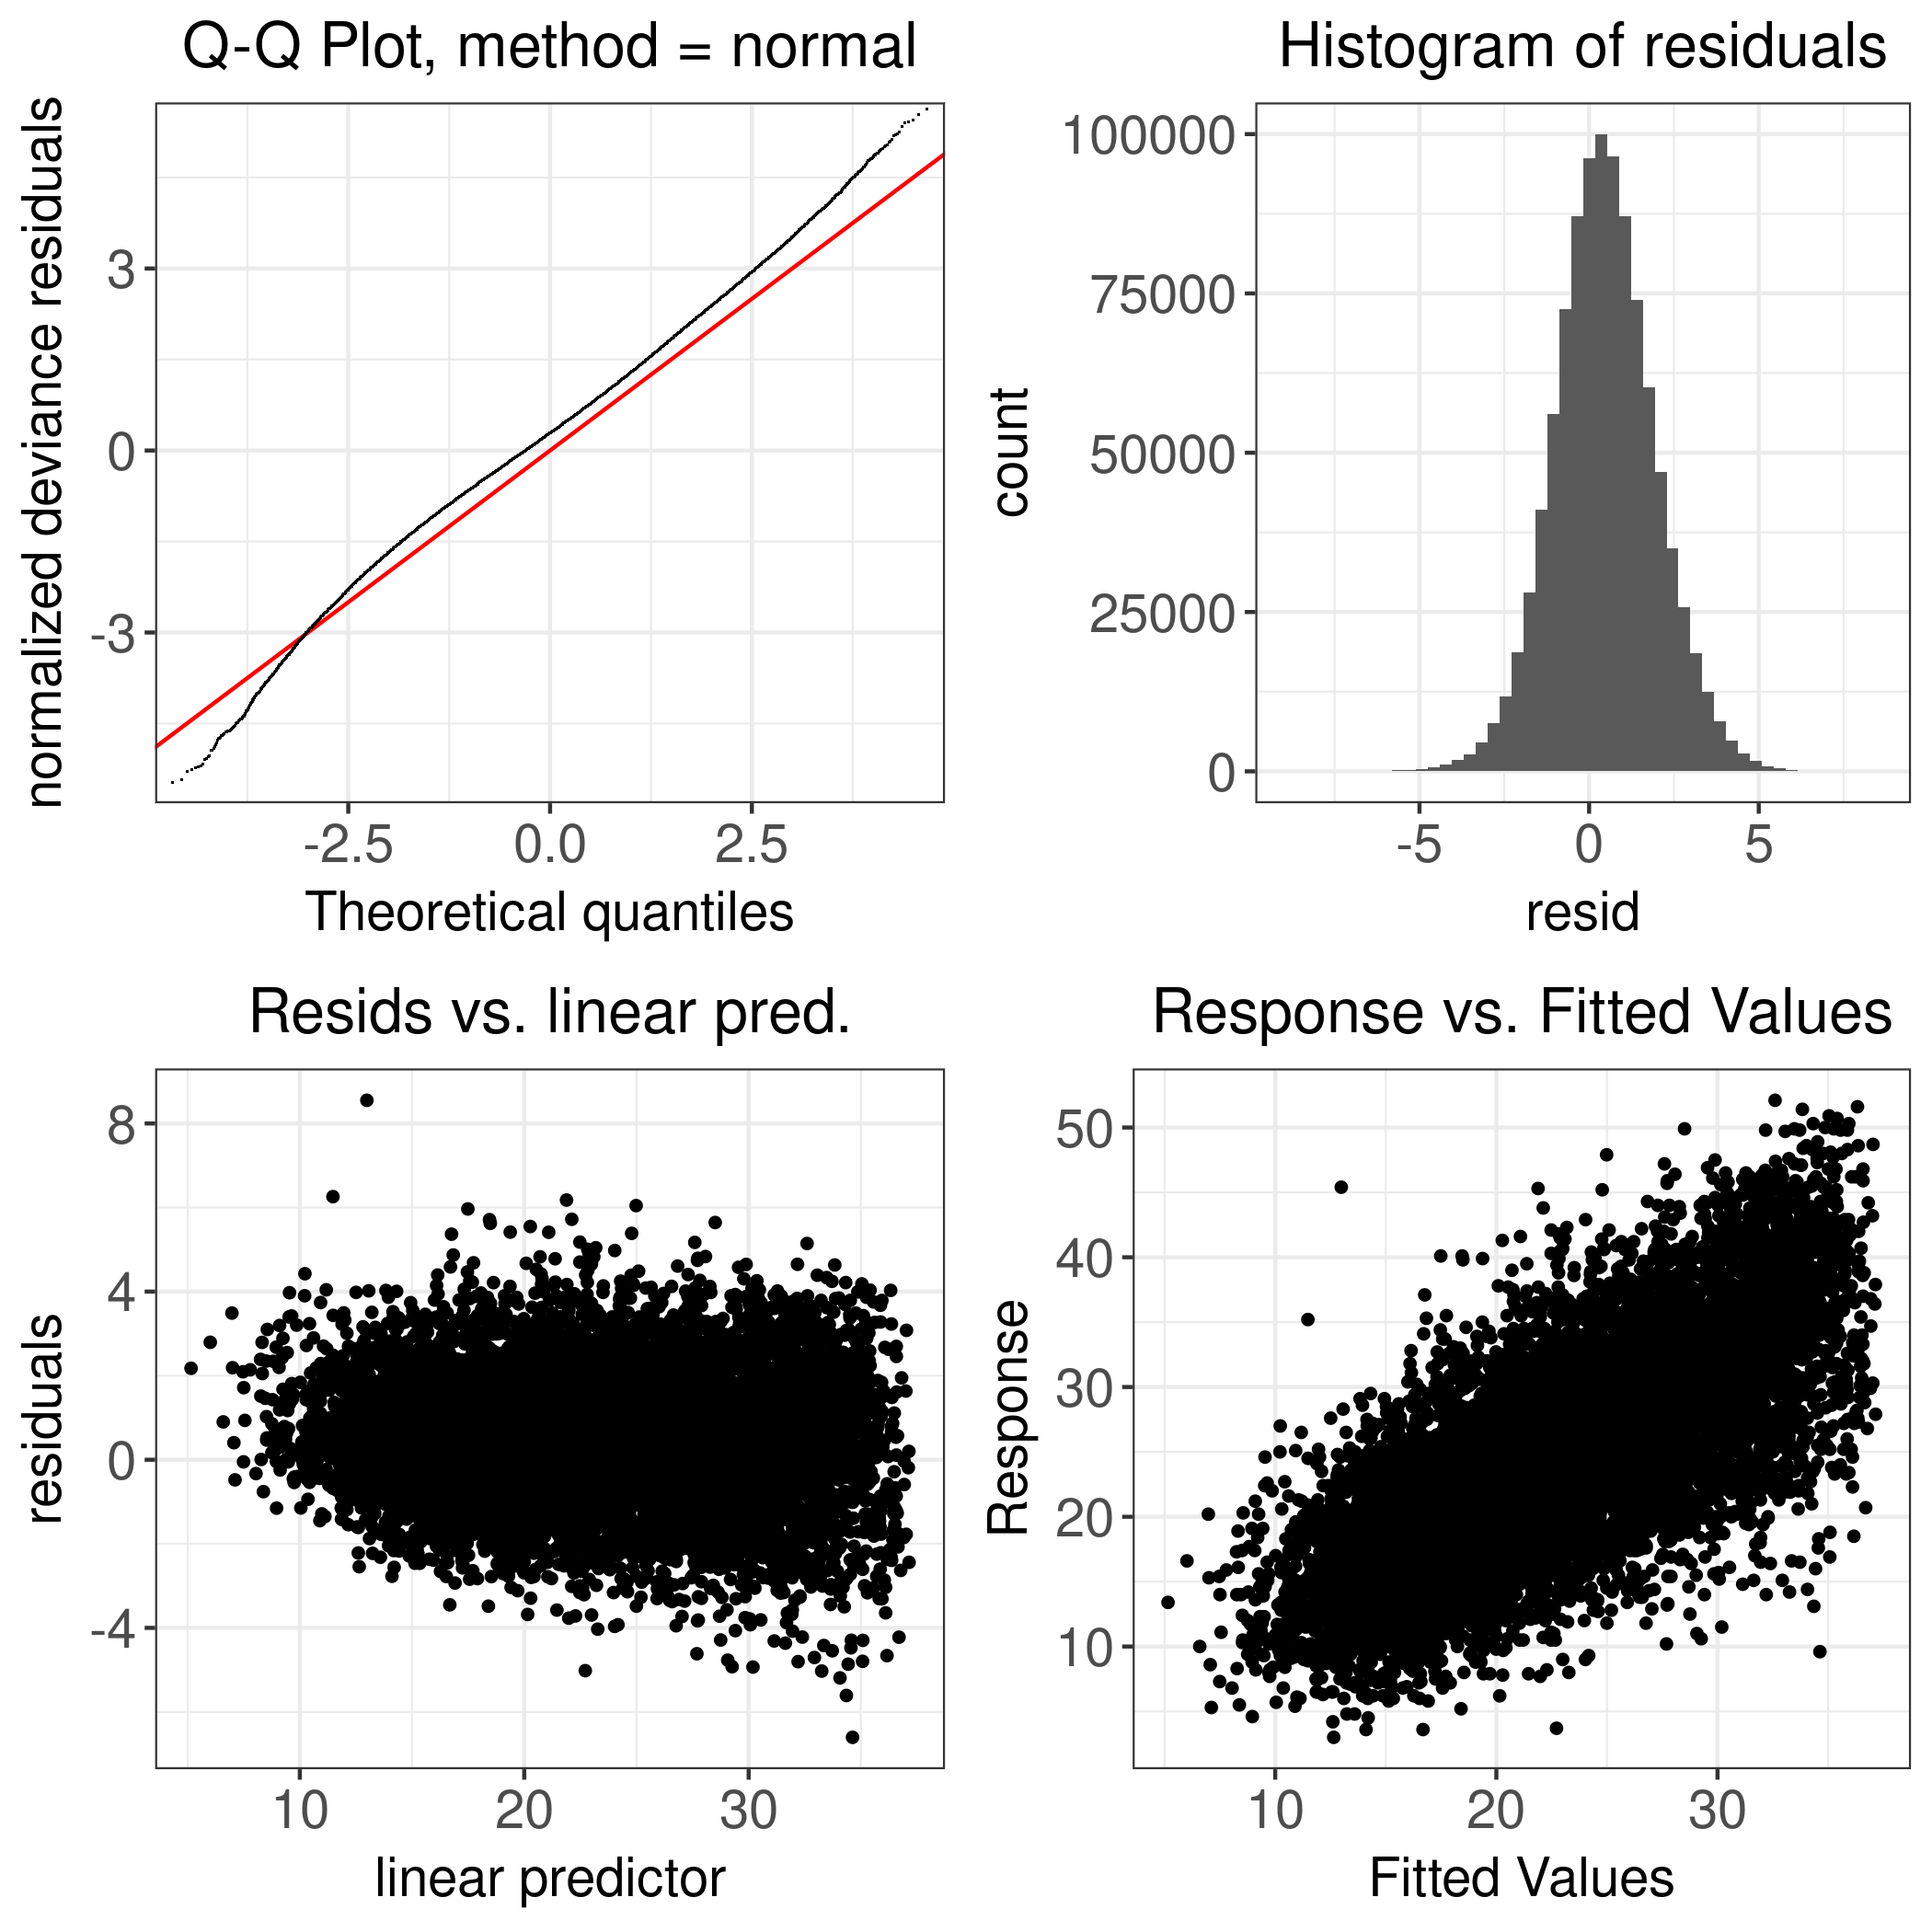
\includegraphics[width=0.6\textwidth]{thesis/figures/models/milk/full/ho_milk_full/ho_milk_full_diagnostics.png}
    \caption[]{Holstein: Milk Yield - 1985-2023 - Diagnostic Plot}
\end{figure}

\newpage
\paragraph{THI Effect and Lactation Curve} \quad \\
\begin{figure}[H]
    \centering
    \begin{subfigure}[b]{0.45\textwidth}
        \centering
        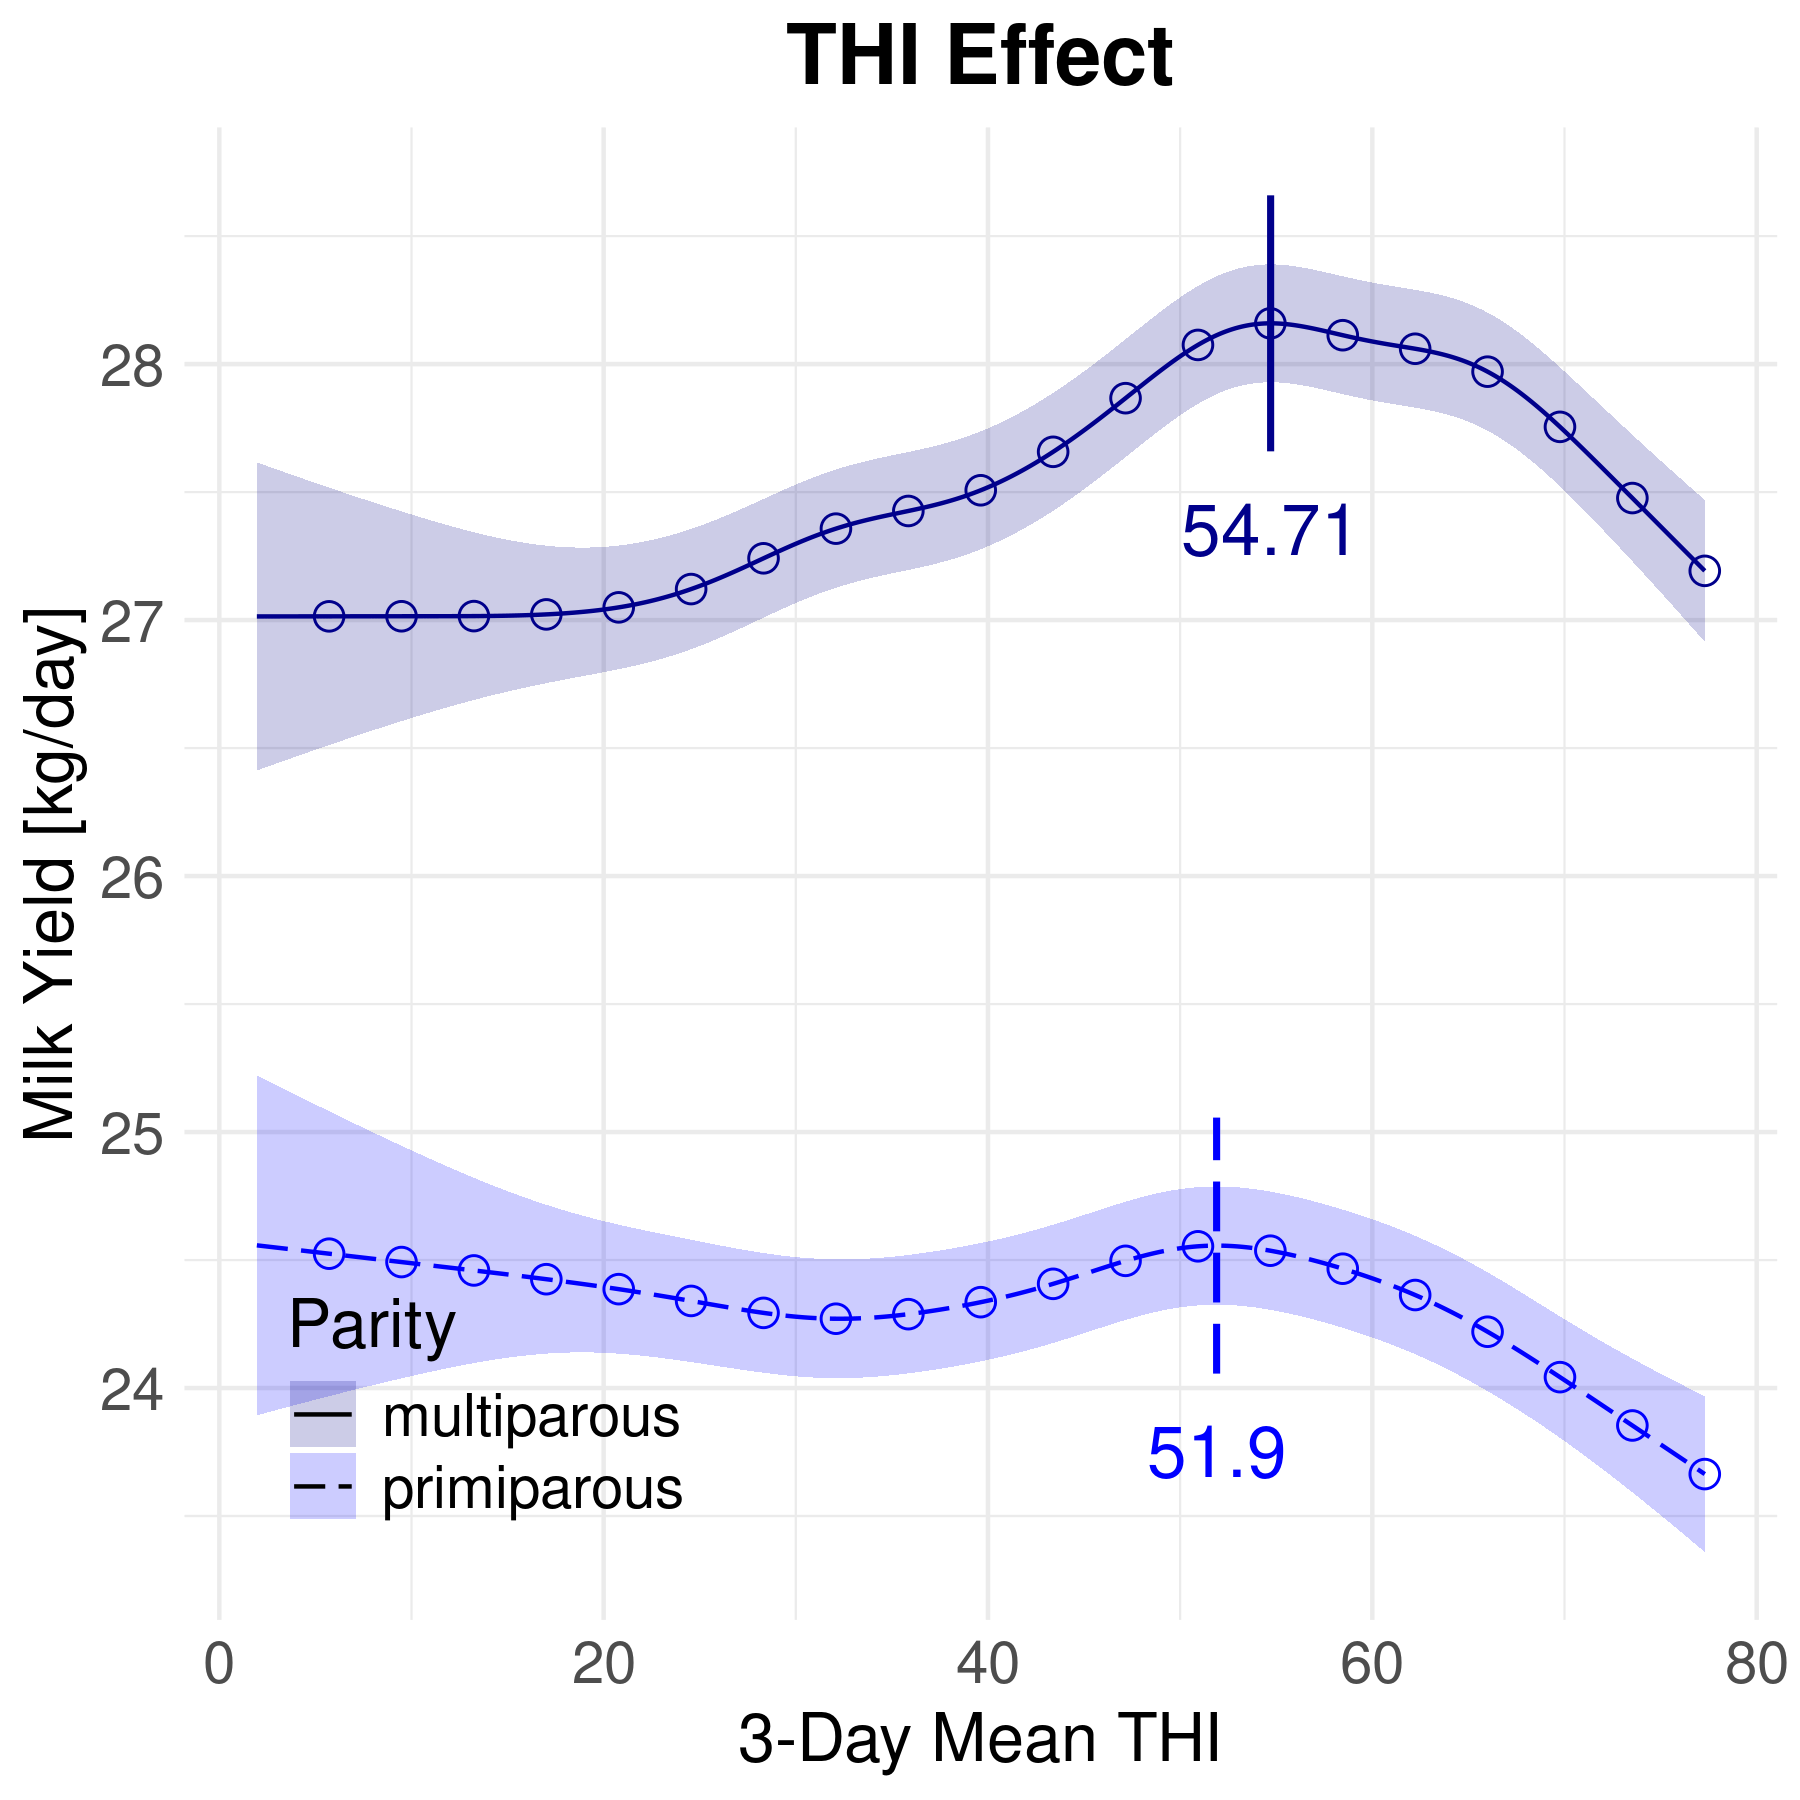
\includegraphics[width=\textwidth]{thesis/figures/models/milk/full/ho_milk_full/ho_milk_full_marginal_thi_milk_combined.png}
    \end{subfigure}
    \hspace{0.05\textwidth} % Optional space between the figures
    \begin{subfigure}[b]{0.45\textwidth}
        \centering
        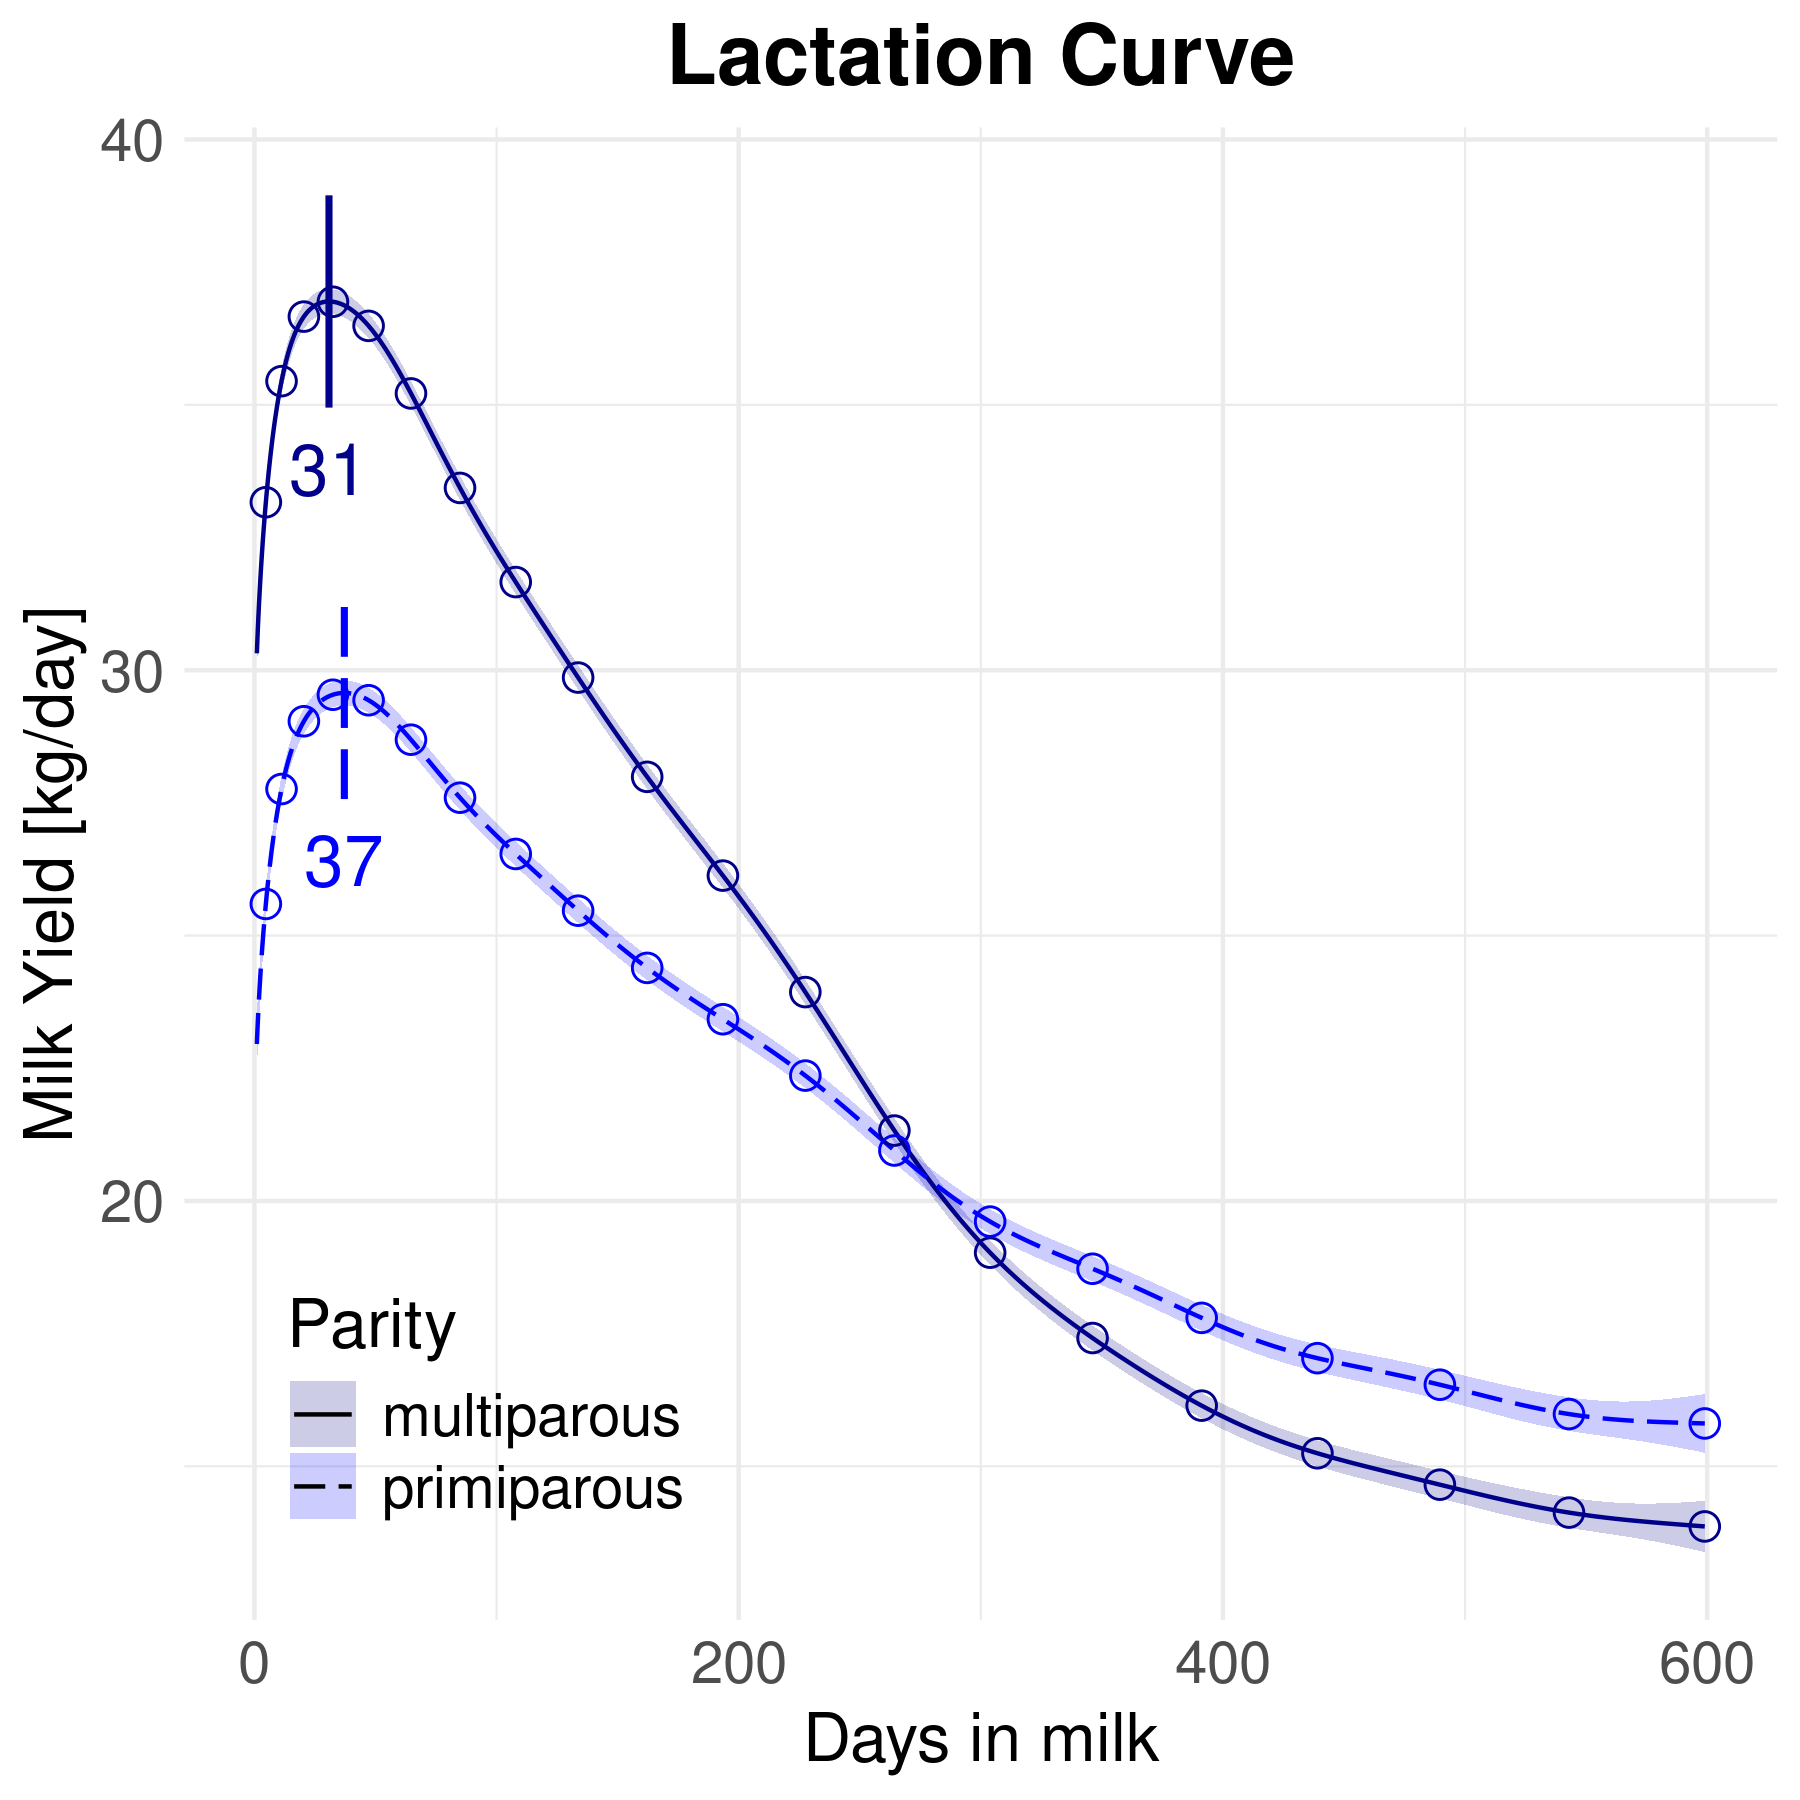
\includegraphics[width=\textwidth]{thesis/figures/models/milk/full/ho_milk_full/ho_milk_full_marginal_dim_milk_combined.png}
    \end{subfigure}
    \begin{subfigure}[b]{0.45\textwidth}
        \centering
        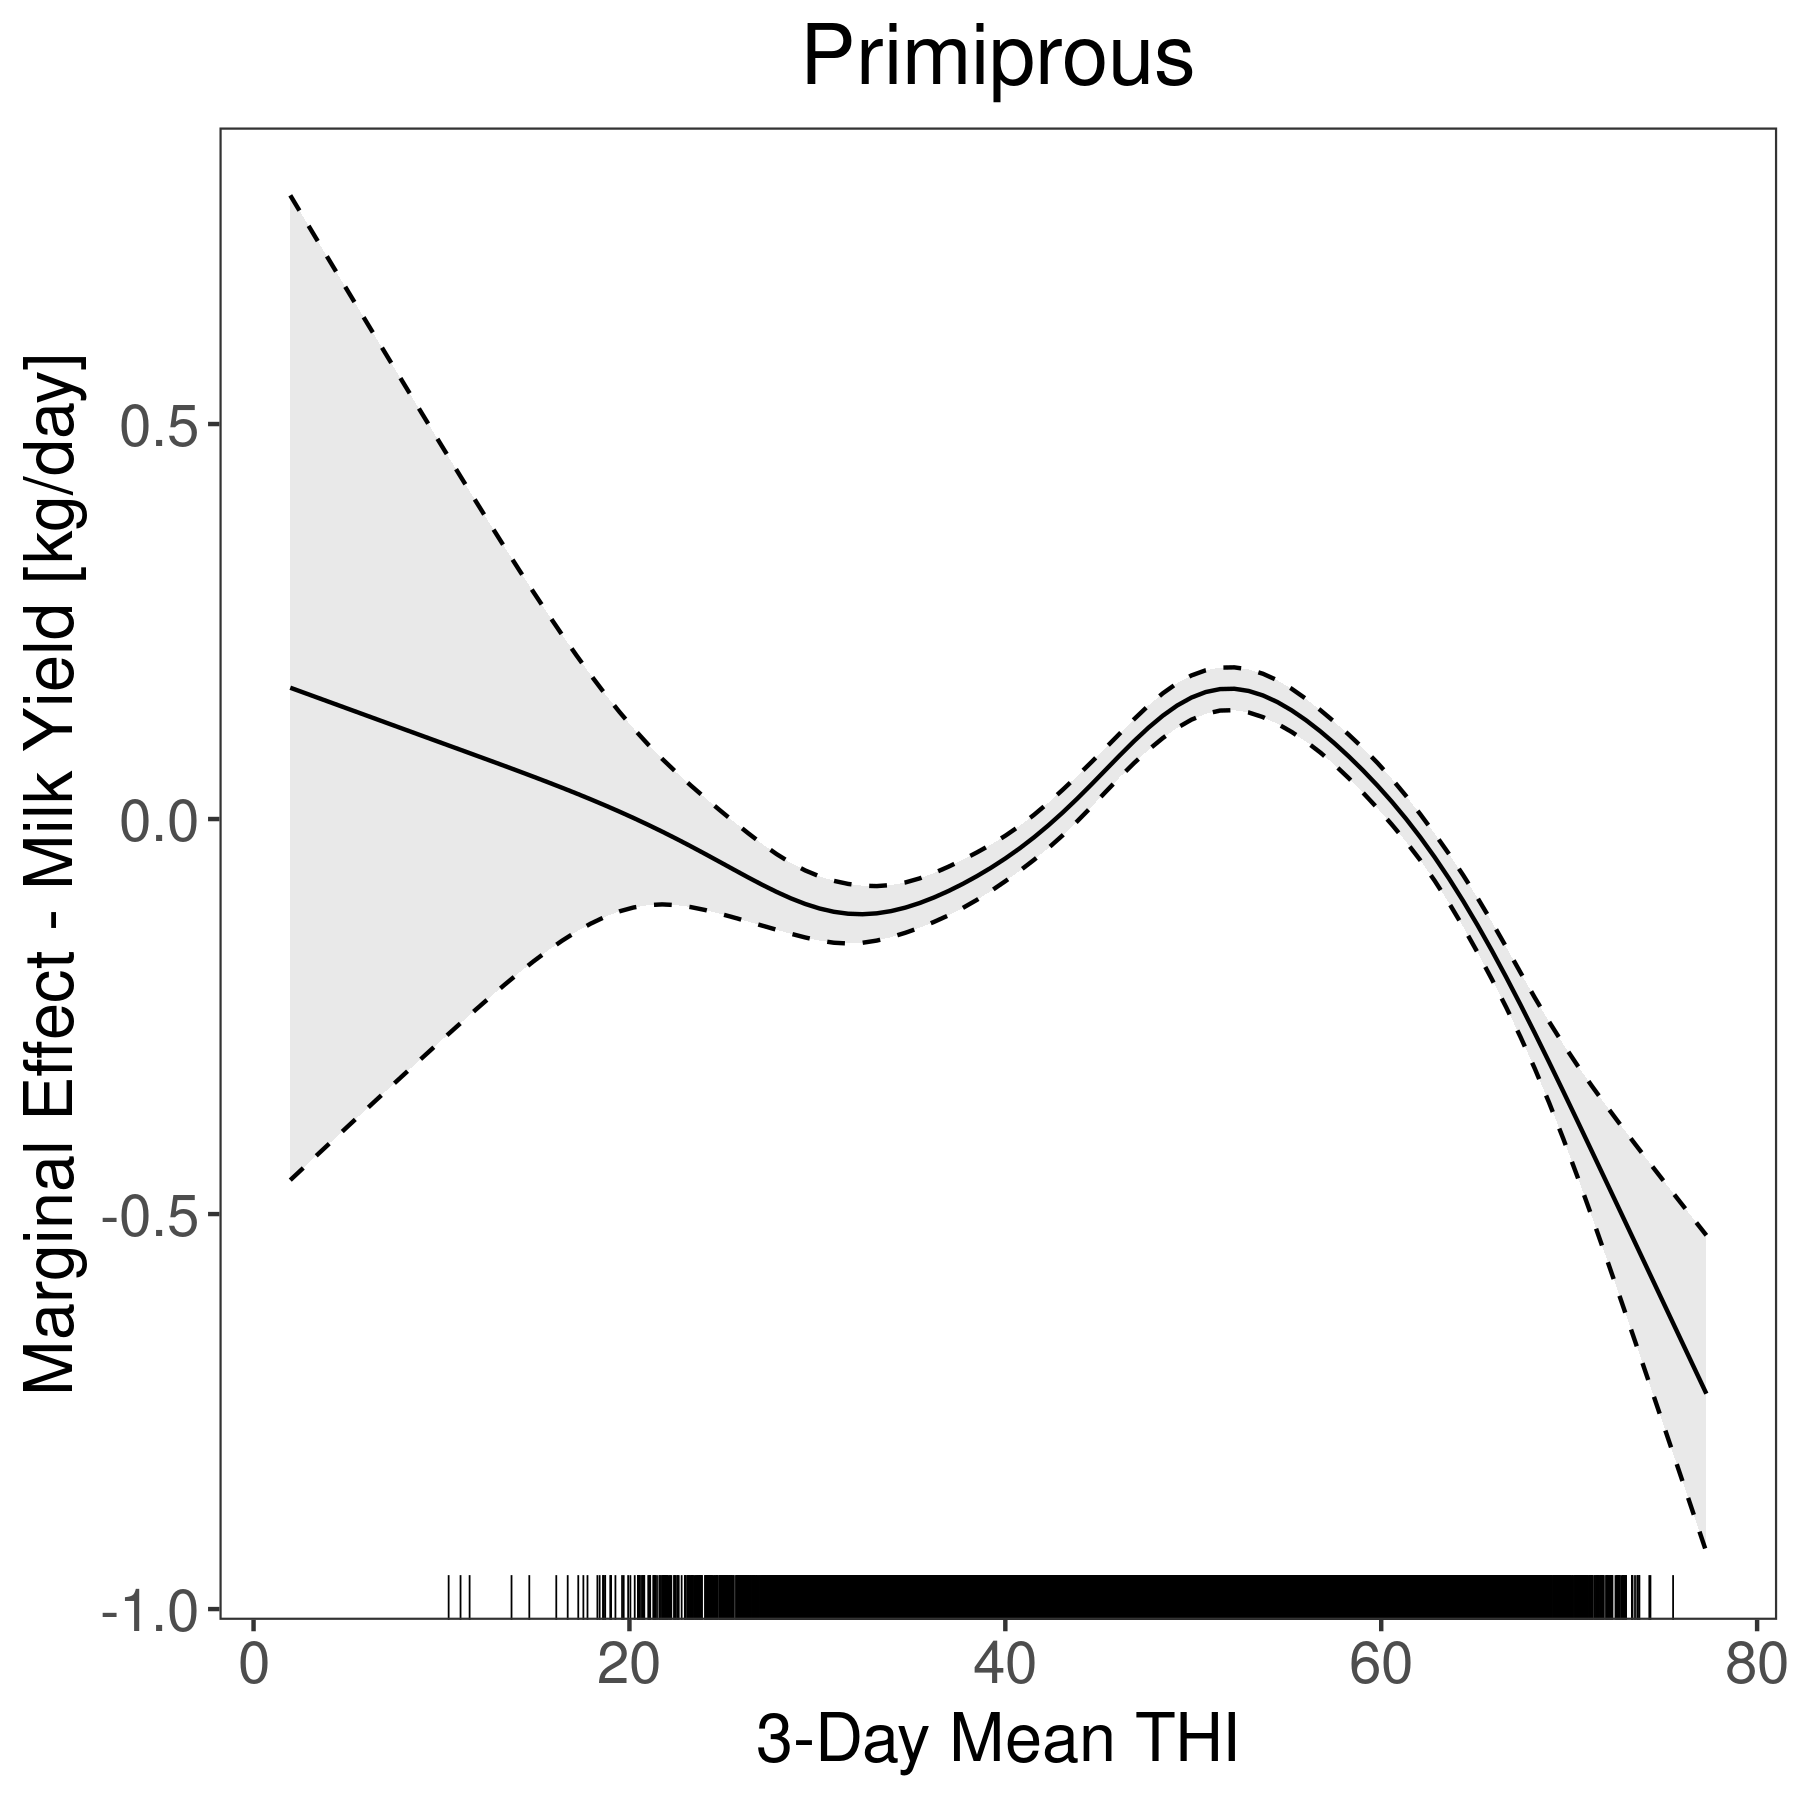
\includegraphics[width=\textwidth]{thesis/figures/models/milk/full/ho_milk_full/ho_milk_full_marginal_thi_milk_primi.png}
    \end{subfigure}
    \hspace{0.05\textwidth} % Optional space between the figures
    \begin{subfigure}[b]{0.45\textwidth}
        \centering
        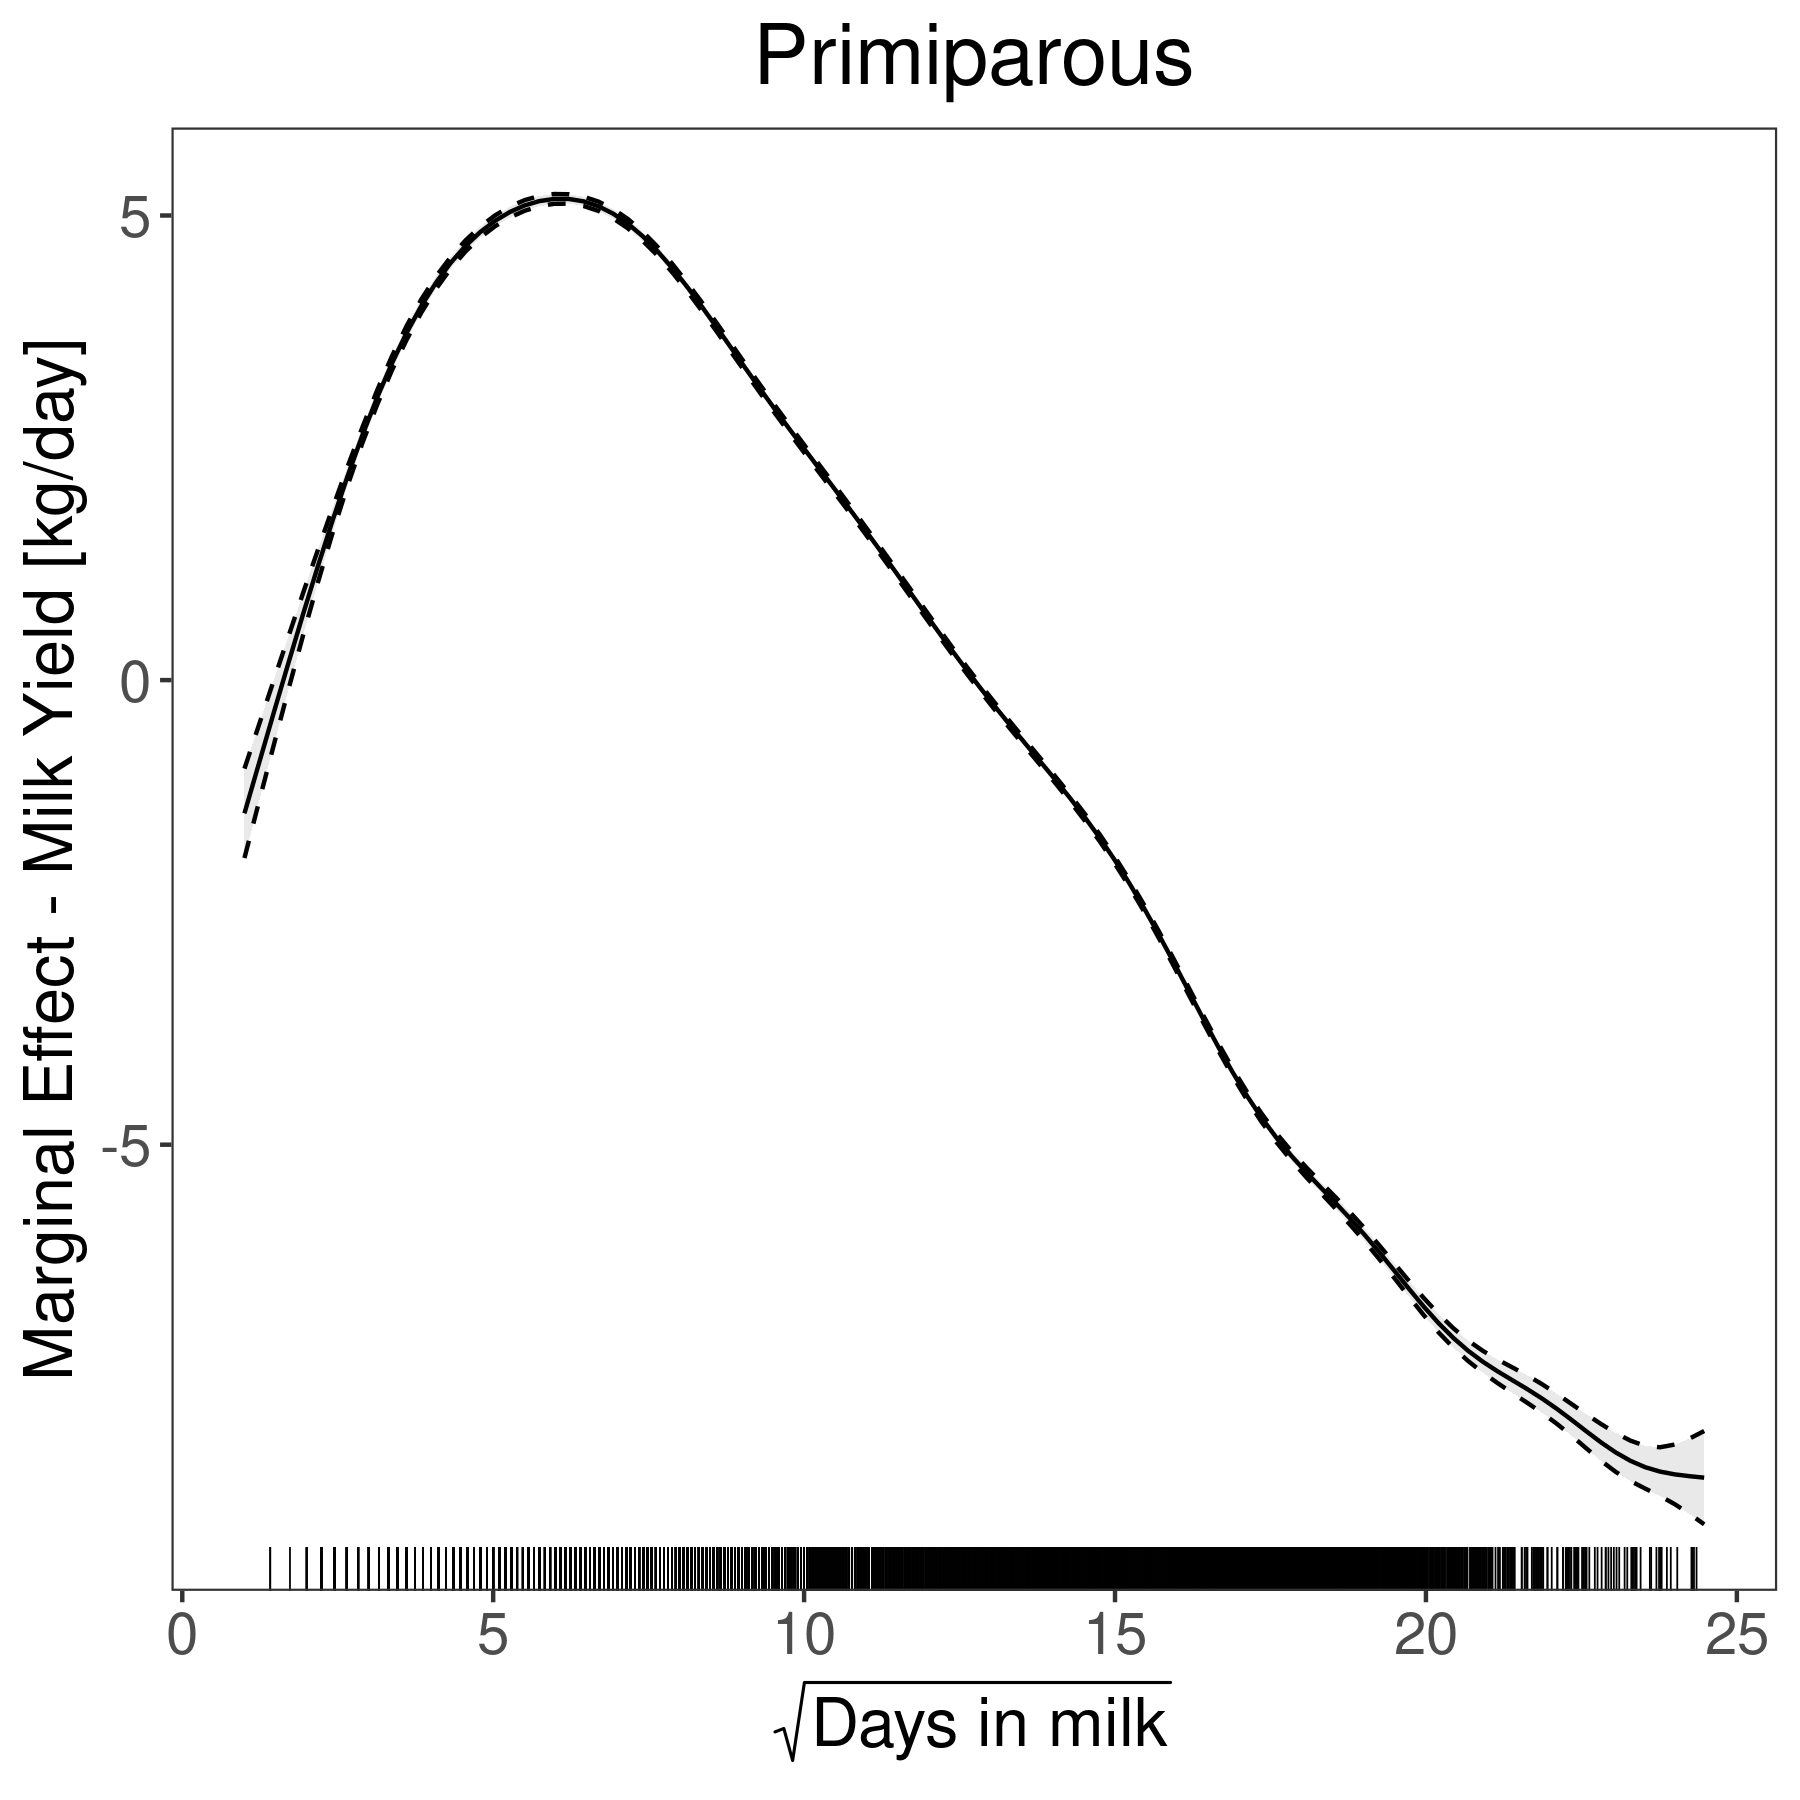
\includegraphics[width=\textwidth]{thesis/figures/models/milk/full/ho_milk_full/ho_milk_full_marginal_dim_milk_primi.png}
    \end{subfigure}
    \begin{subfigure}[b]{0.45\textwidth}
        \centering
        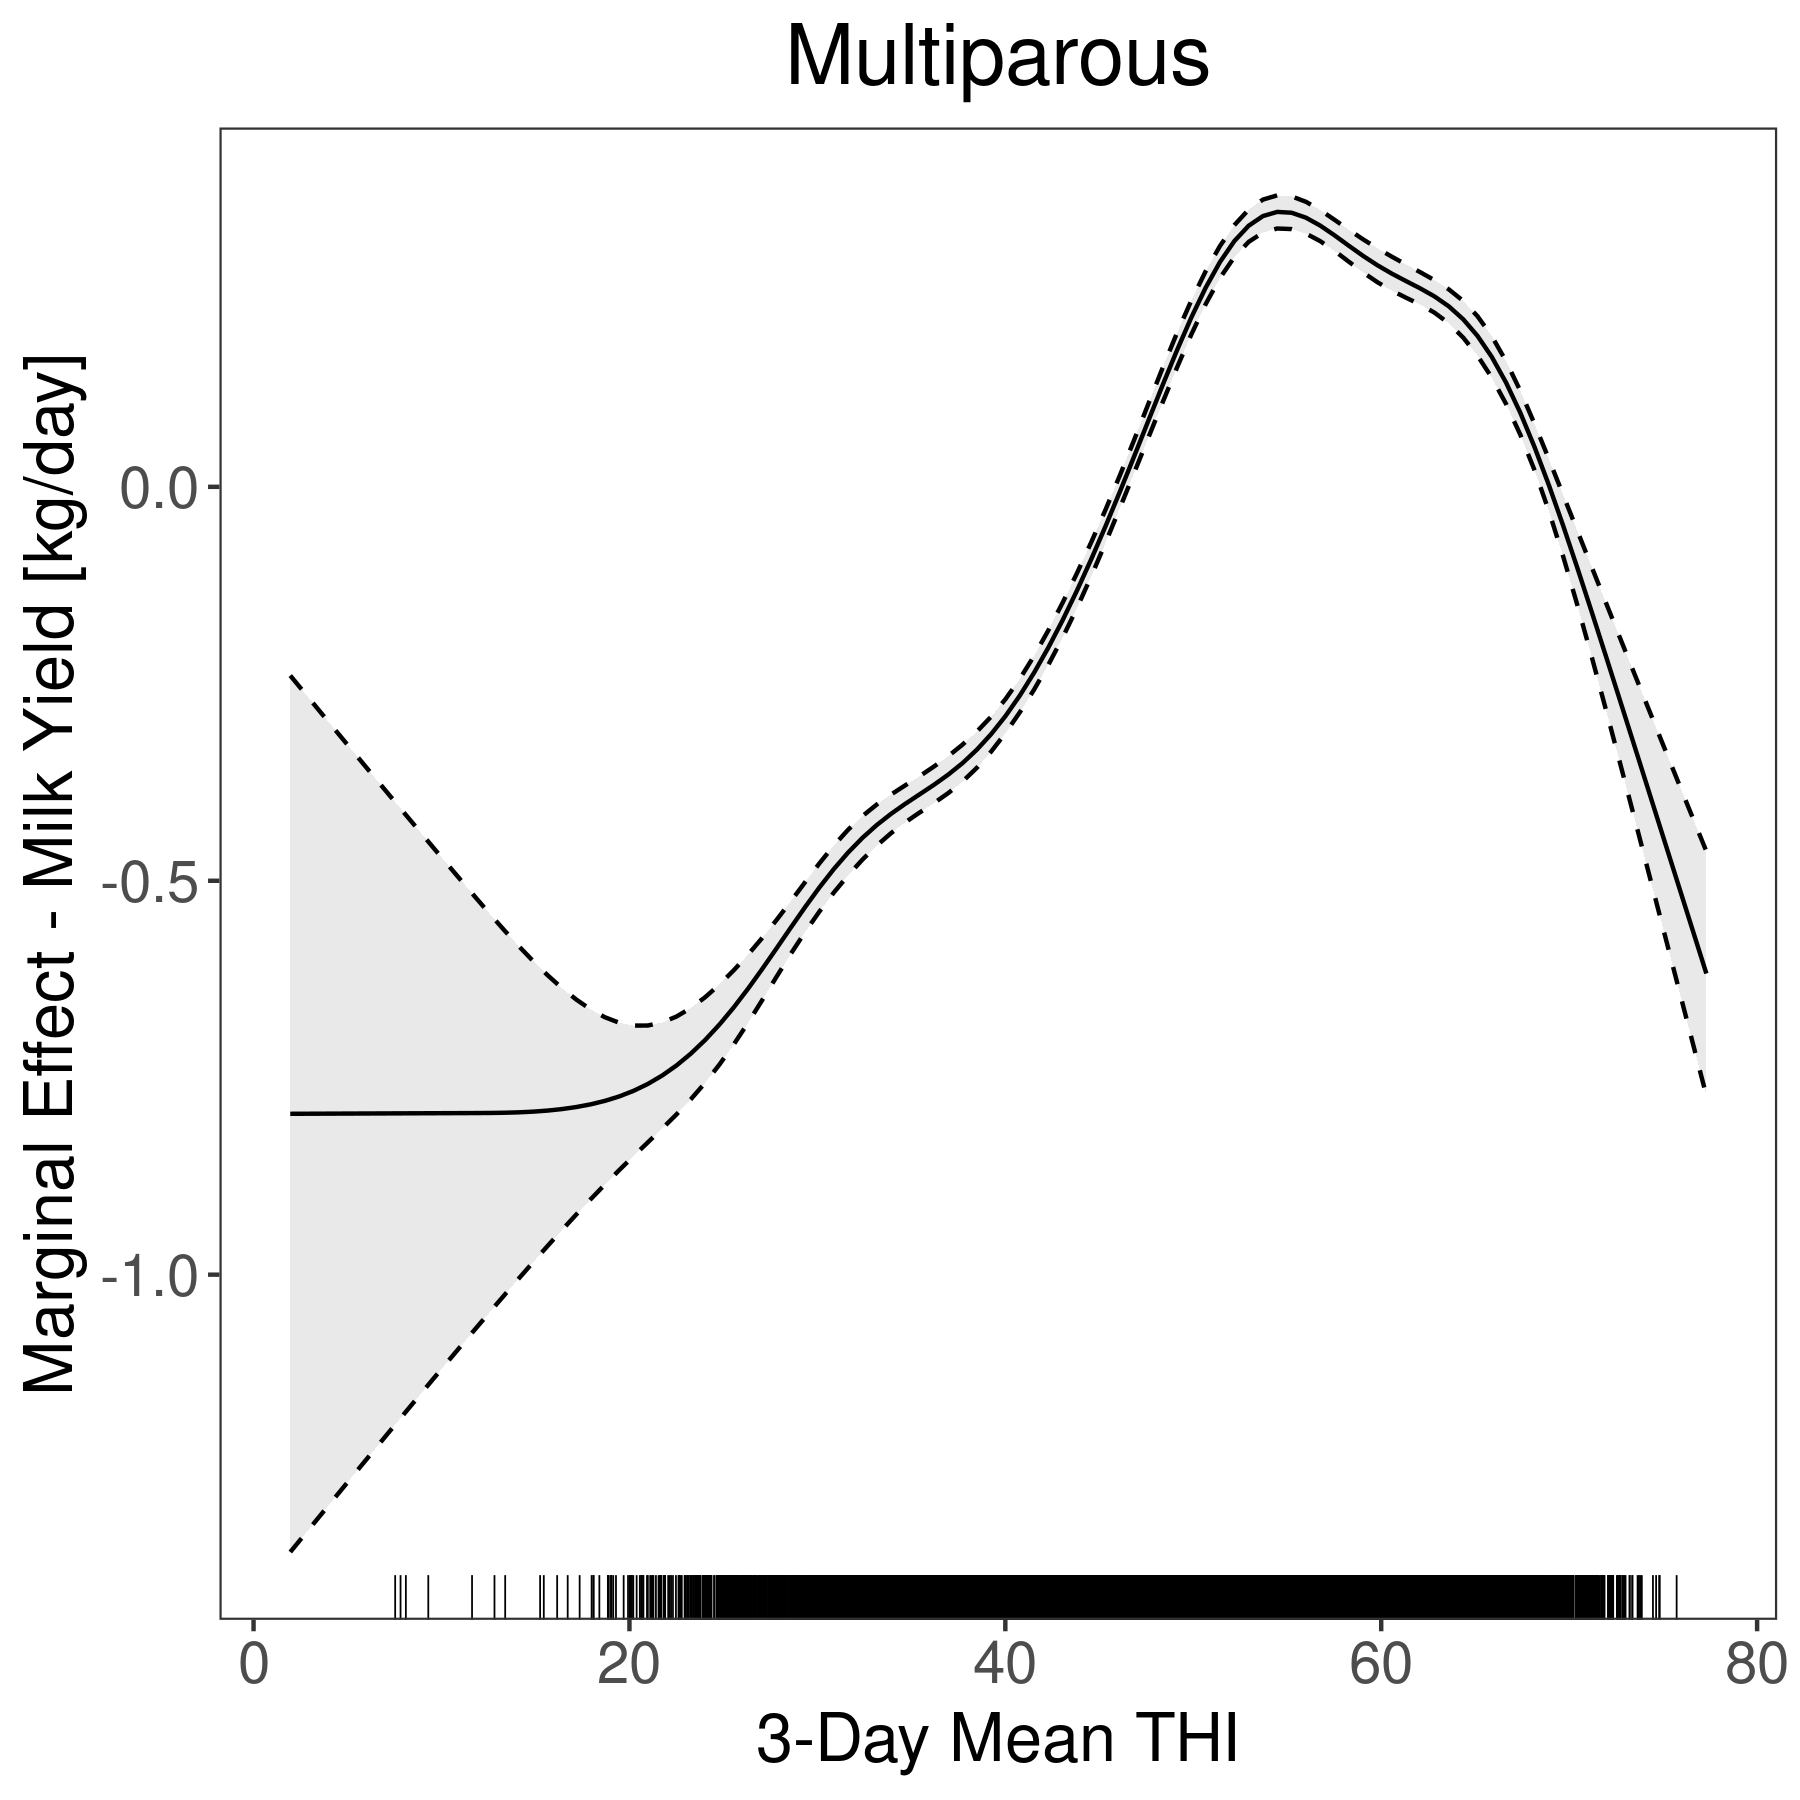
\includegraphics[width=\textwidth]{thesis/figures/models/milk/full/ho_milk_full/ho_milk_full_marginal_thi_milk_multi.png}
    \end{subfigure}
    \hspace{0.05\textwidth} % Optional space between the figures
    \begin{subfigure}[b]{0.45\textwidth}
        \centering
        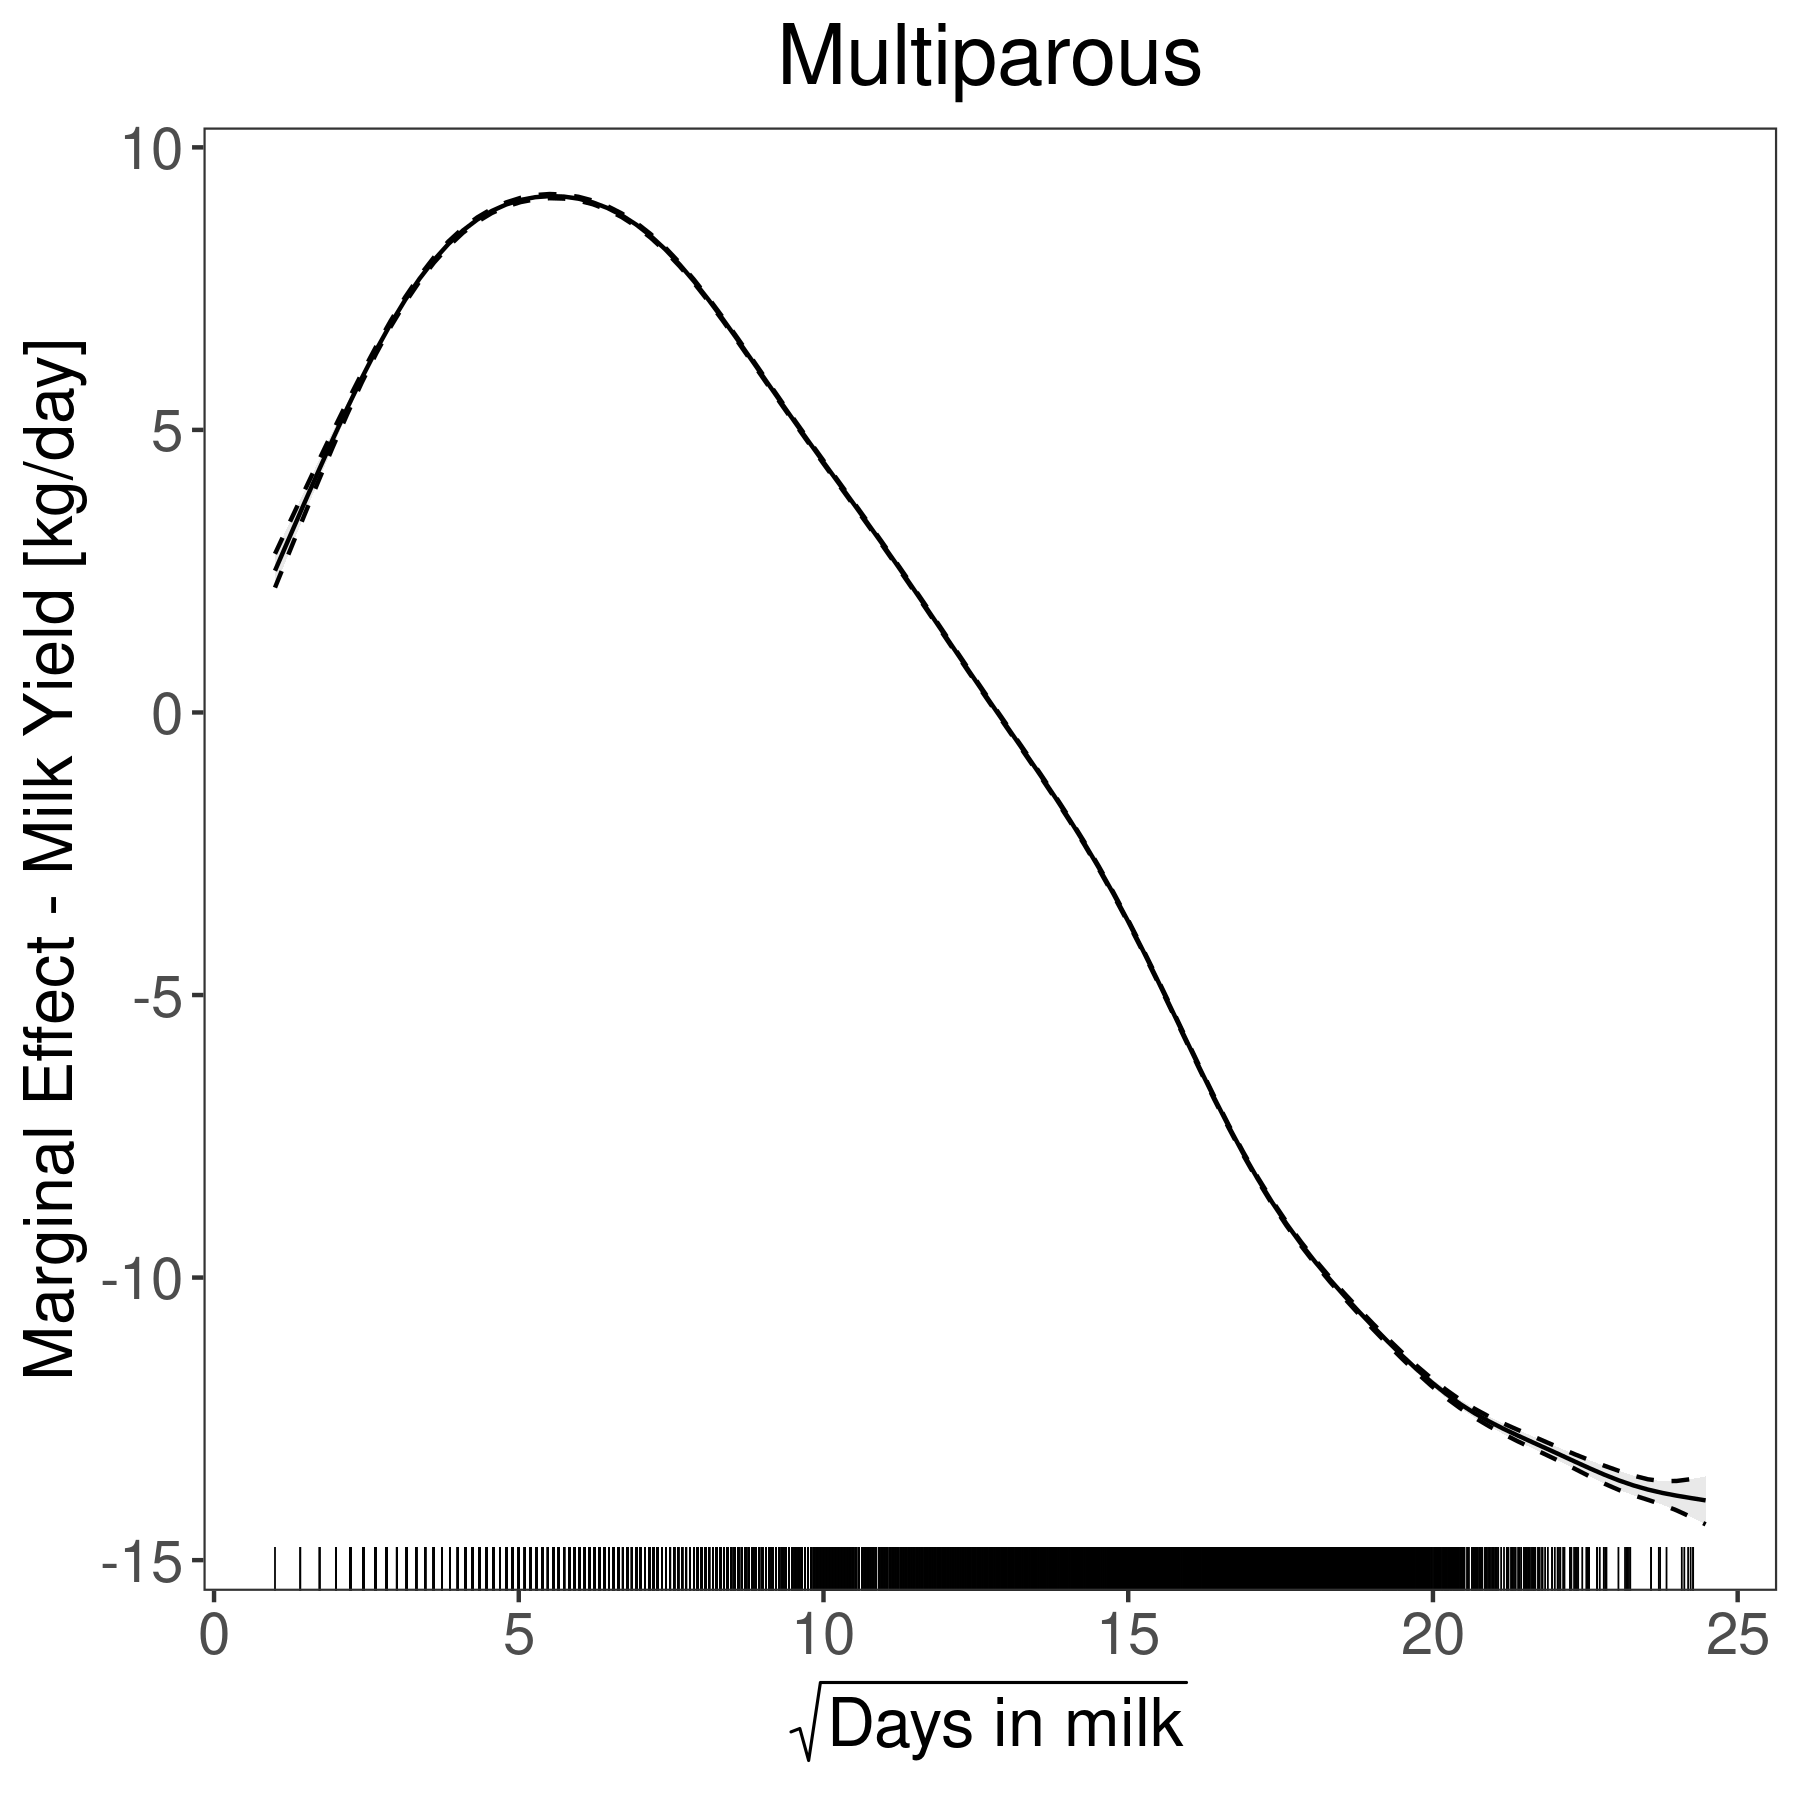
\includegraphics[width=\textwidth]{thesis/figures/models/milk/full/ho_milk_full/ho_milk_full_marginal_dim_milk_multi.png}
    \end{subfigure}
    \caption[]{Holstein: Milk Yield - 1985 - 2023 - THI Effect and Lactation Curve}
    \label{fig:main}
\end{figure}

\subsection{Split Period: Until 2010 - After 2010}
\addtocontents{toc}{\protect\setcounter{tocdepth}{-1}}
\subsubsection{Split Period: 1985 - 2010}\label{model:ho_milk_before}
\paragraph{Model Summary} \quad \\

    \begin{table}[H]
    \centering
    \begin{tabular}{lrrrr}
    \textbf{A. parametric coefficients} & Estimate & Std. Error & t-value & p-value \\ 
       \hline
       \hline
  (Intercept) & 17.4723 & 0.4846 & 36.0518 & $<$ 0.0001 \\ 
  parityprimiparous & -2.9636 & 0.0135 & -218.8244 & $<$ 0.0001 \\ 
  year1986 & 0.1529 & 0.1767 & 0.8655 & 0.3868 \\ 
  year1987 & -0.0051 & 0.3698 & -0.0139 & 0.9889 \\ 
  year1988 & -0.0538 & 0.4676 & -0.1151 & 0.9084 \\ 
  year1989 & 0.5836 & 0.5228 & 1.1162 & 0.2643 \\ 
  year1990 & 1.0427 & 0.5324 & 1.9586 & 0.0502 \\ 
  year1991 & 1.2681 & 0.5365 & 2.3638 & 0.0181 \\ 
  year1992 & 1.5385 & 0.5405 & 2.8462 & 0.0044 \\ 
  year1993 & 1.7418 & 0.5397 & 3.2271 & 0.0013 \\ 
  year1994 & 1.7286 & 0.5424 & 3.1867 & 0.0014 \\ 
  year1995 & 2.0734 & 0.5756 & 3.6019 & 0.0003 \\ 
  year1996 & 2.2707 & 0.5748 & 3.9506 & 0.0001 \\ 
  year1997 & 2.7340 & 0.5549 & 4.9272 & $<$ 0.0001 \\ 
  year1998 & 3.3217 & 0.5222 & 6.3608 & $<$ 0.0001 \\ 
  year1999 & 3.4296 & 0.5187 & 6.6121 & $<$ 0.0001 \\ 
  year2000 & 3.6071 & 0.5113 & 7.0543 & $<$ 0.0001 \\ 
  year2001 & 3.9367 & 0.5104 & 7.7127 & $<$ 0.0001 \\ 
  year2002 & 4.2369 & 0.5132 & 8.2562 & $<$ 0.0001 \\ 
  year2003 & 4.7670 & 0.5144 & 9.2674 & $<$ 0.0001 \\ 
  year2004 & 5.2638 & 0.5135 & 10.2511 & $<$ 0.0001 \\ 
  year2005 & 5.7675 & 0.5124 & 11.2567 & $<$ 0.0001 \\ 
  year2006 & 5.9112 & 0.5147 & 11.4841 & $<$ 0.0001 \\ 
  year2007 & 5.8929 & 0.5097 & 11.5607 & $<$ 0.0001 \\ 
  year2008 & 6.2882 & 0.4996 & 12.5867 & $<$ 0.0001 \\ 
  year2009 & 6.9956 & 0.5079 & 13.7748 & $<$ 0.0001 \\ 
  year2010 & 7.7149 & 0.5678 & 13.5864 & $<$ 0.0001 \\ 
       \hline
    \textbf{B. smooth terms} & edf & Ref.df & F-value & p-value \\ 
    \hline
    \hline
  s(thi\_mean\_t0\_3d):paritymultiparous & 8.5121 & 8.5121 & 747.8886 & $<$ 0.0001 \\ 
  s(thi\_mean\_t0\_3d):parityprimiparous & 7.1550 & 7.1550 & 77.0589 & $<$ 0.0001 \\ 
  s(days\_in\_milk\_t):paritymultiparous & 14.4063 & 14.4063 & 130999.6058 & $<$ 0.0001 \\ 
  s(days\_in\_milk\_t):parityprimiparous & 13.8961 & 13.8961 & 17856.8448 & $<$ 0.0001 \\ 
       \hline
    \end{tabular}
    \caption[]{Holstein: Milk Yield - 1985-2010 - GAMM model summary without random effect terms.}
    \end{table}

\newpage
\begin{table}[H]
\centering
\begin{tabular}
{l | r | r | r | r}
\textbf{Smooth Term Fixed Effect} & Est. & SE & z & p\\
\hline
\hline
s(thi\_mean\_t0\_3d):multiFx1 & -0.5301 & 0.1141 & -4.65 & $<$ 1e-05\\
s(thi\_mean\_t0\_3d):primiFx1 & -0.3337 & 0.1241 & -2.69 & 0.0072\\
s(days\_in\_milk\_):multiFx1 & 2.4075 & 0.5902 & 4.08 & $<$ 1e-04\\
s(days\_in\_milk\_):primiFx1 & 2.9462 & 0.6274 & 4.70 & $<$ 1e-05\\
\hline
\textbf{Variance Component} & Estimated $\sigma$ & & & \\
\hline
\hline
$\sigma_\alpha$ & 2.9738 & &  & \\
$\sigma_\iota$ & 0.9483 & & & \\
$\sigma_\phi$ & 2.7446 & & & \\
s(thi\_mean\_t0\_3d):multi & 2.7246 & & & \\
s(days\_in\_milk\_):primi & 7.6254 & & & \\
s(days\_in\_milk\_):multi & 9.4602 & & & \\
s(thi\_mean\_t0\_3d):primi & 1.5465 & & & \\
Residual & 3.4568 & & & \\
\end{tabular}
\caption[]{Holstein: Milk Yield - 1985-2010 - Mixed Model Summary - Smooth Terms and Random Effects.}
\end{table}

\paragraph{Model Diagnostics} \quad \\
\begin{figure}[H]
    \centering
    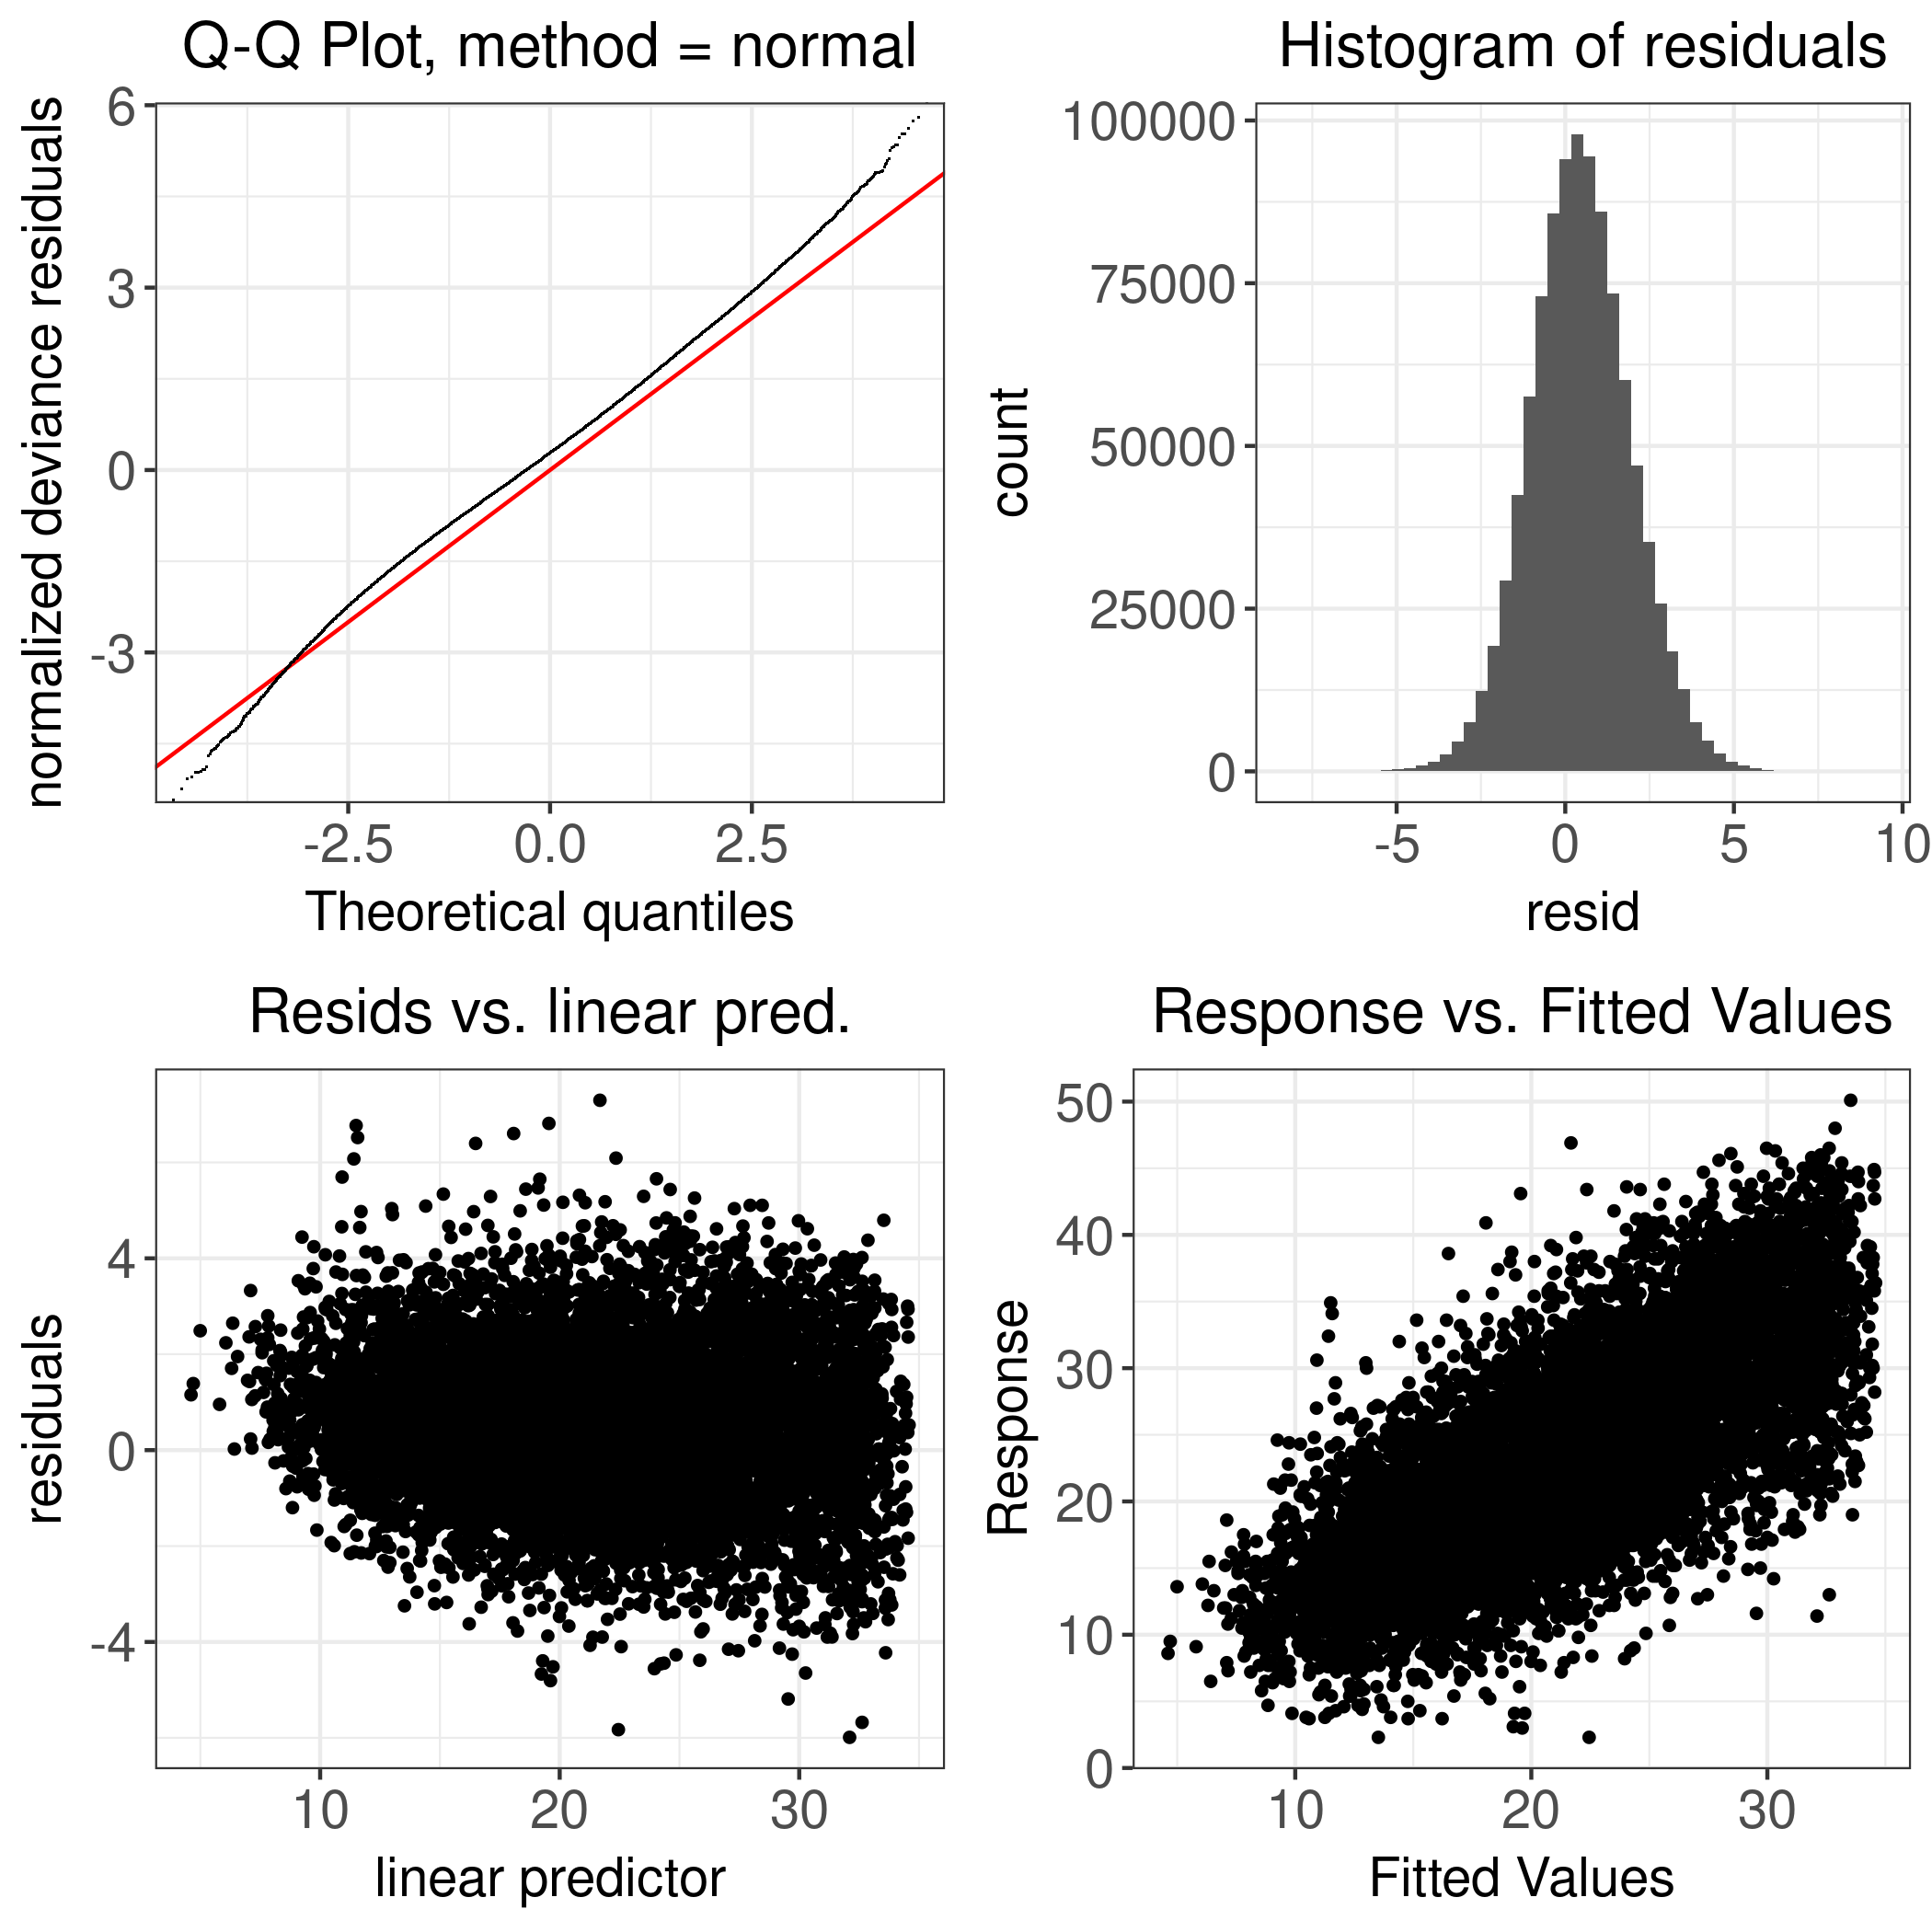
\includegraphics[width=0.6\textwidth]{thesis/figures/models/milk/before2010/ho_milk_before2010/ho_milk_before2010_diagnostics.png}
    \caption[]{Holstein: Milk Yield - 1985-2010 - Diagnostic Plot}
\end{figure}

\newpage
\paragraph{THI Effect and Lactation Curve} \quad \\
\begin{figure}[H]
    \centering
    \begin{subfigure}[b]{0.45\textwidth}
        \centering
        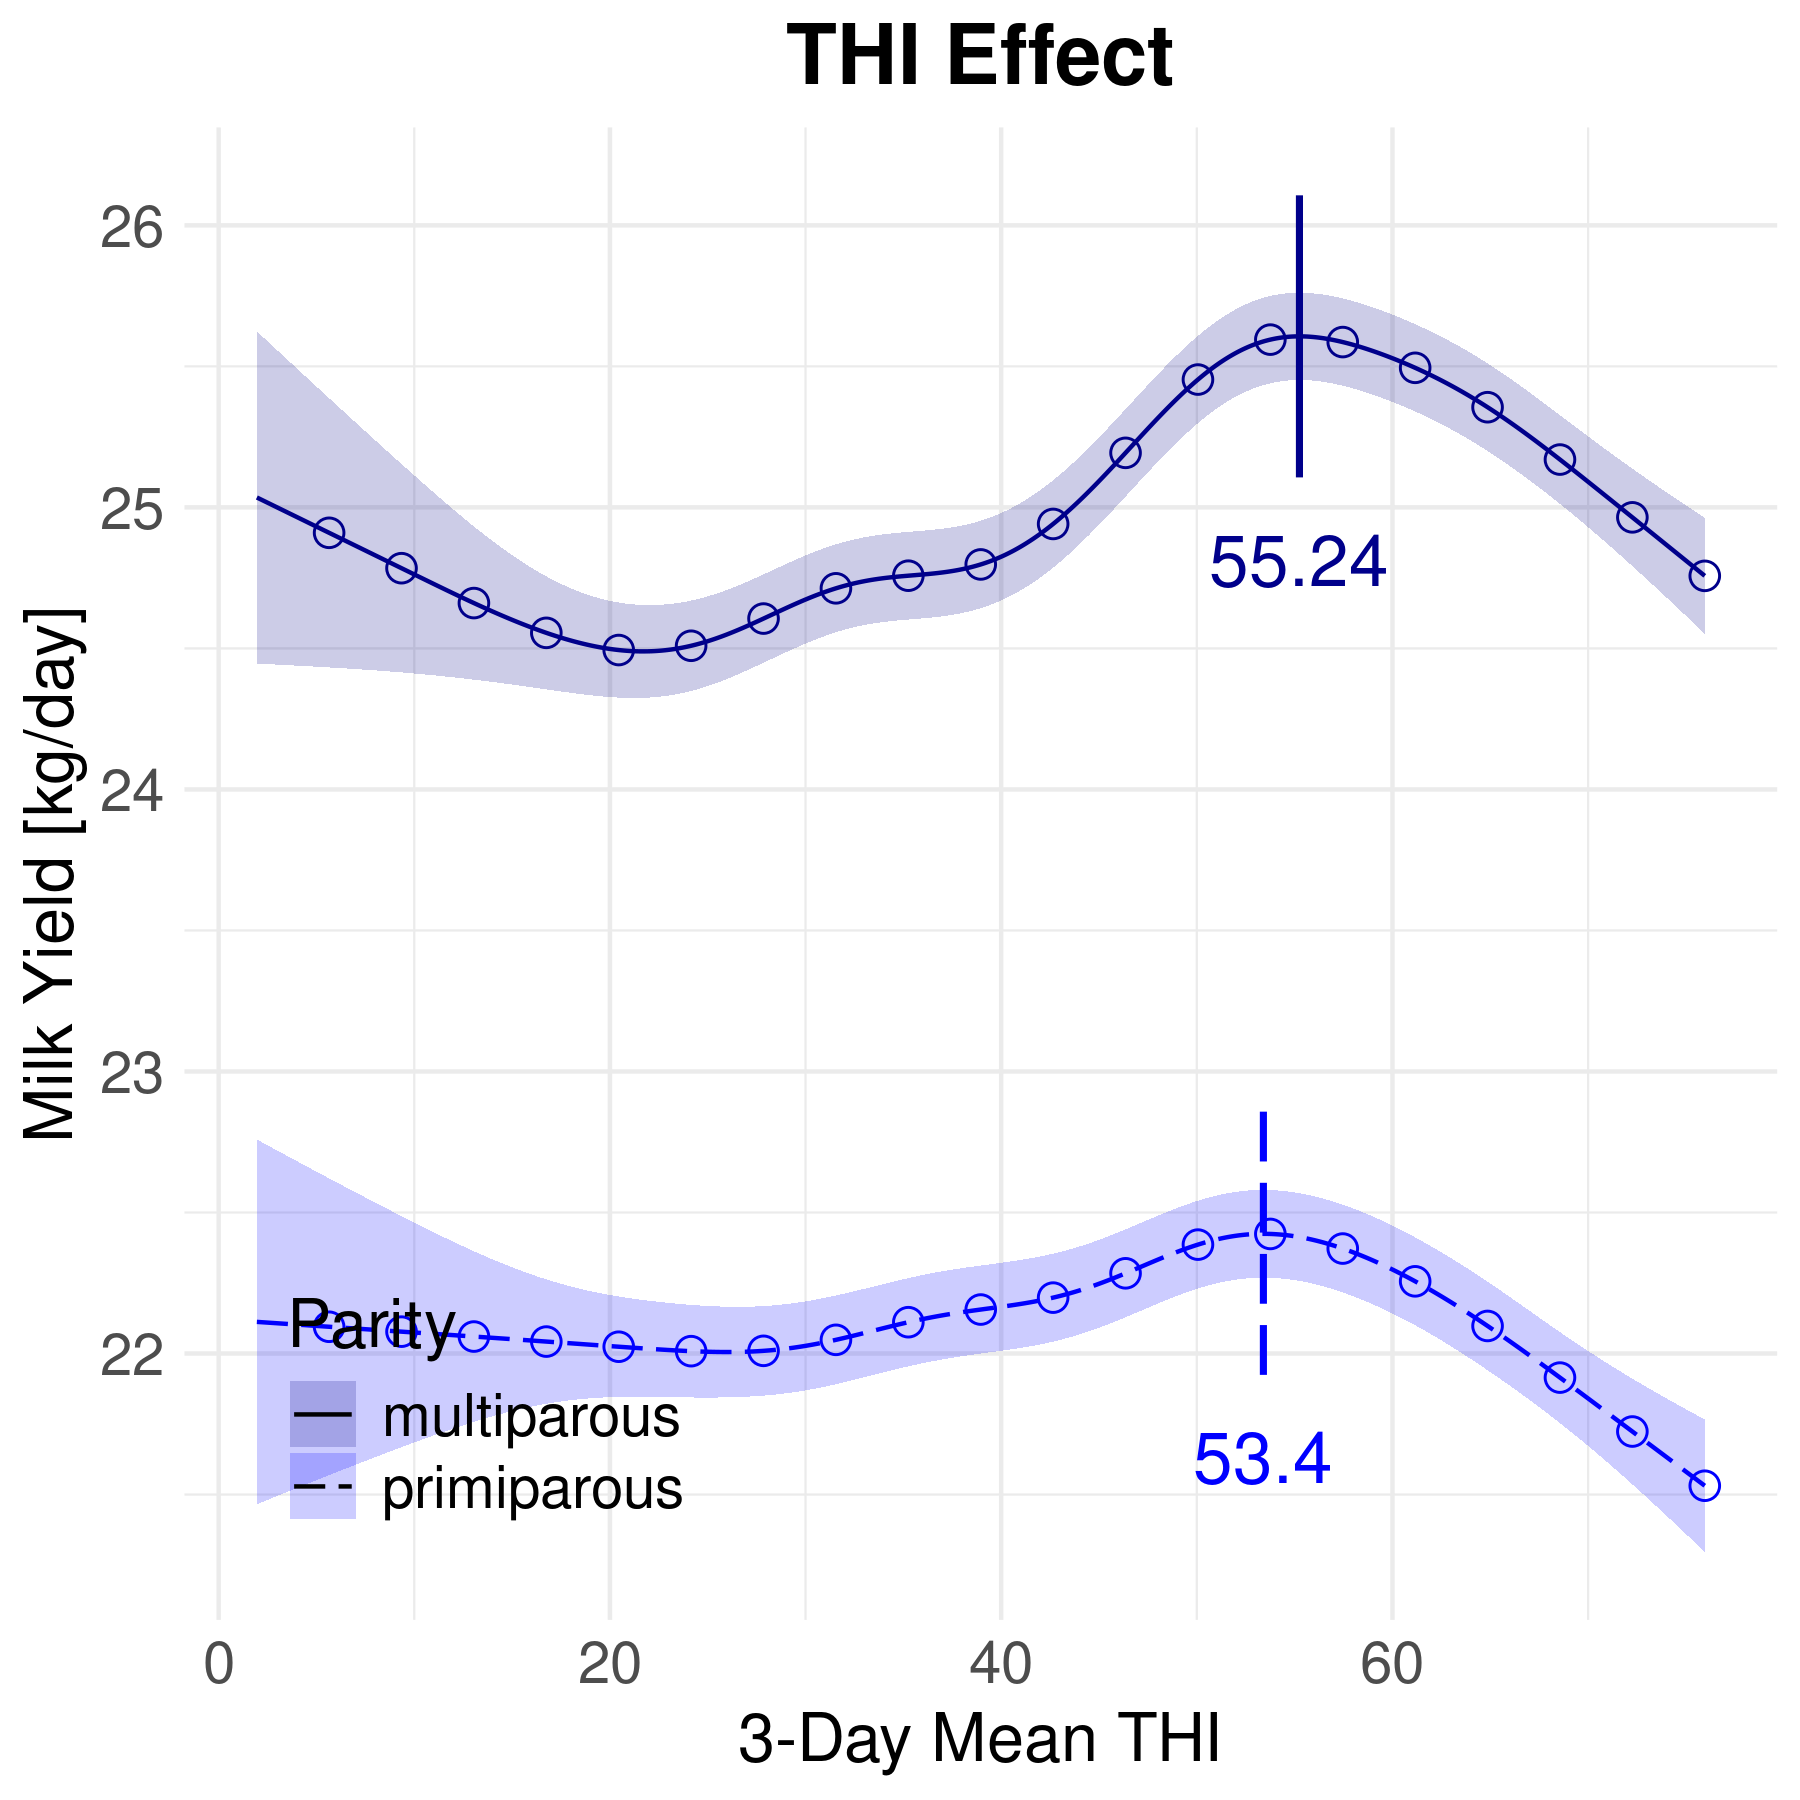
\includegraphics[width=\textwidth]{thesis/figures/models/milk/before2010/ho_milk_before2010/ho_milk_before2010_marginal_thi_milk_combined.png}
    \end{subfigure}
    \hspace{0.05\textwidth} % Optional space between the figures
    \begin{subfigure}[b]{0.45\textwidth}
        \centering
        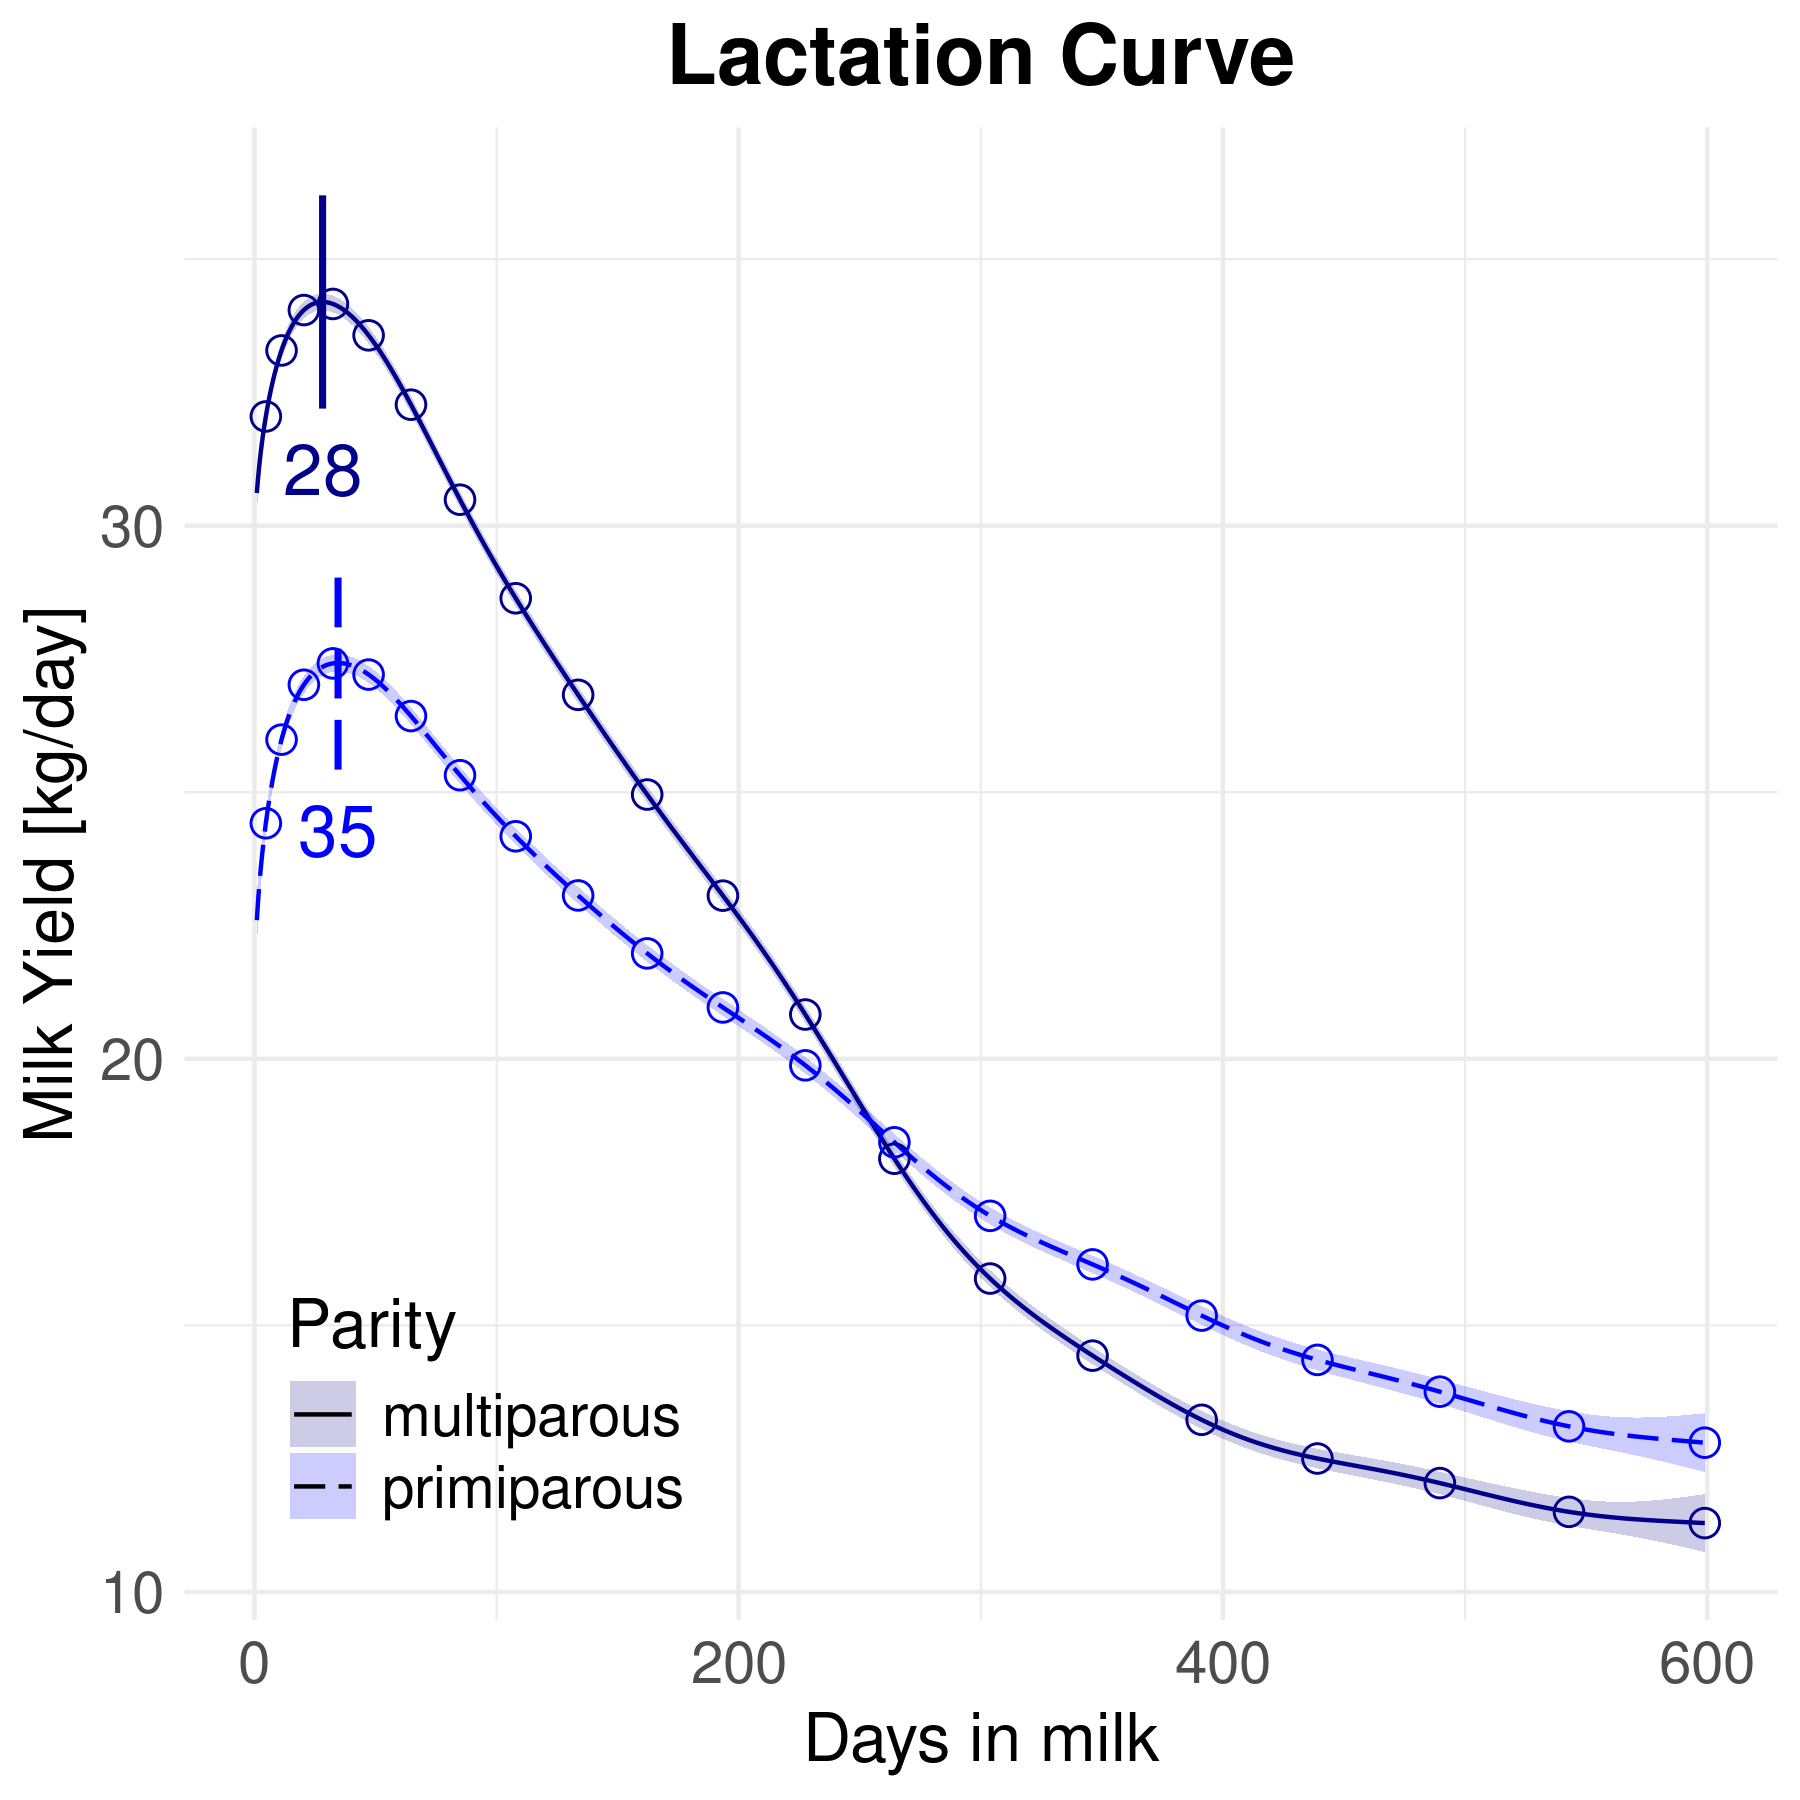
\includegraphics[width=\textwidth]{thesis/figures/models/milk/before2010/ho_milk_before2010/ho_milk_before2010_marginal_dim_milk_combined.png}
    \end{subfigure}
    \begin{subfigure}[b]{0.45\textwidth}
        \centering
        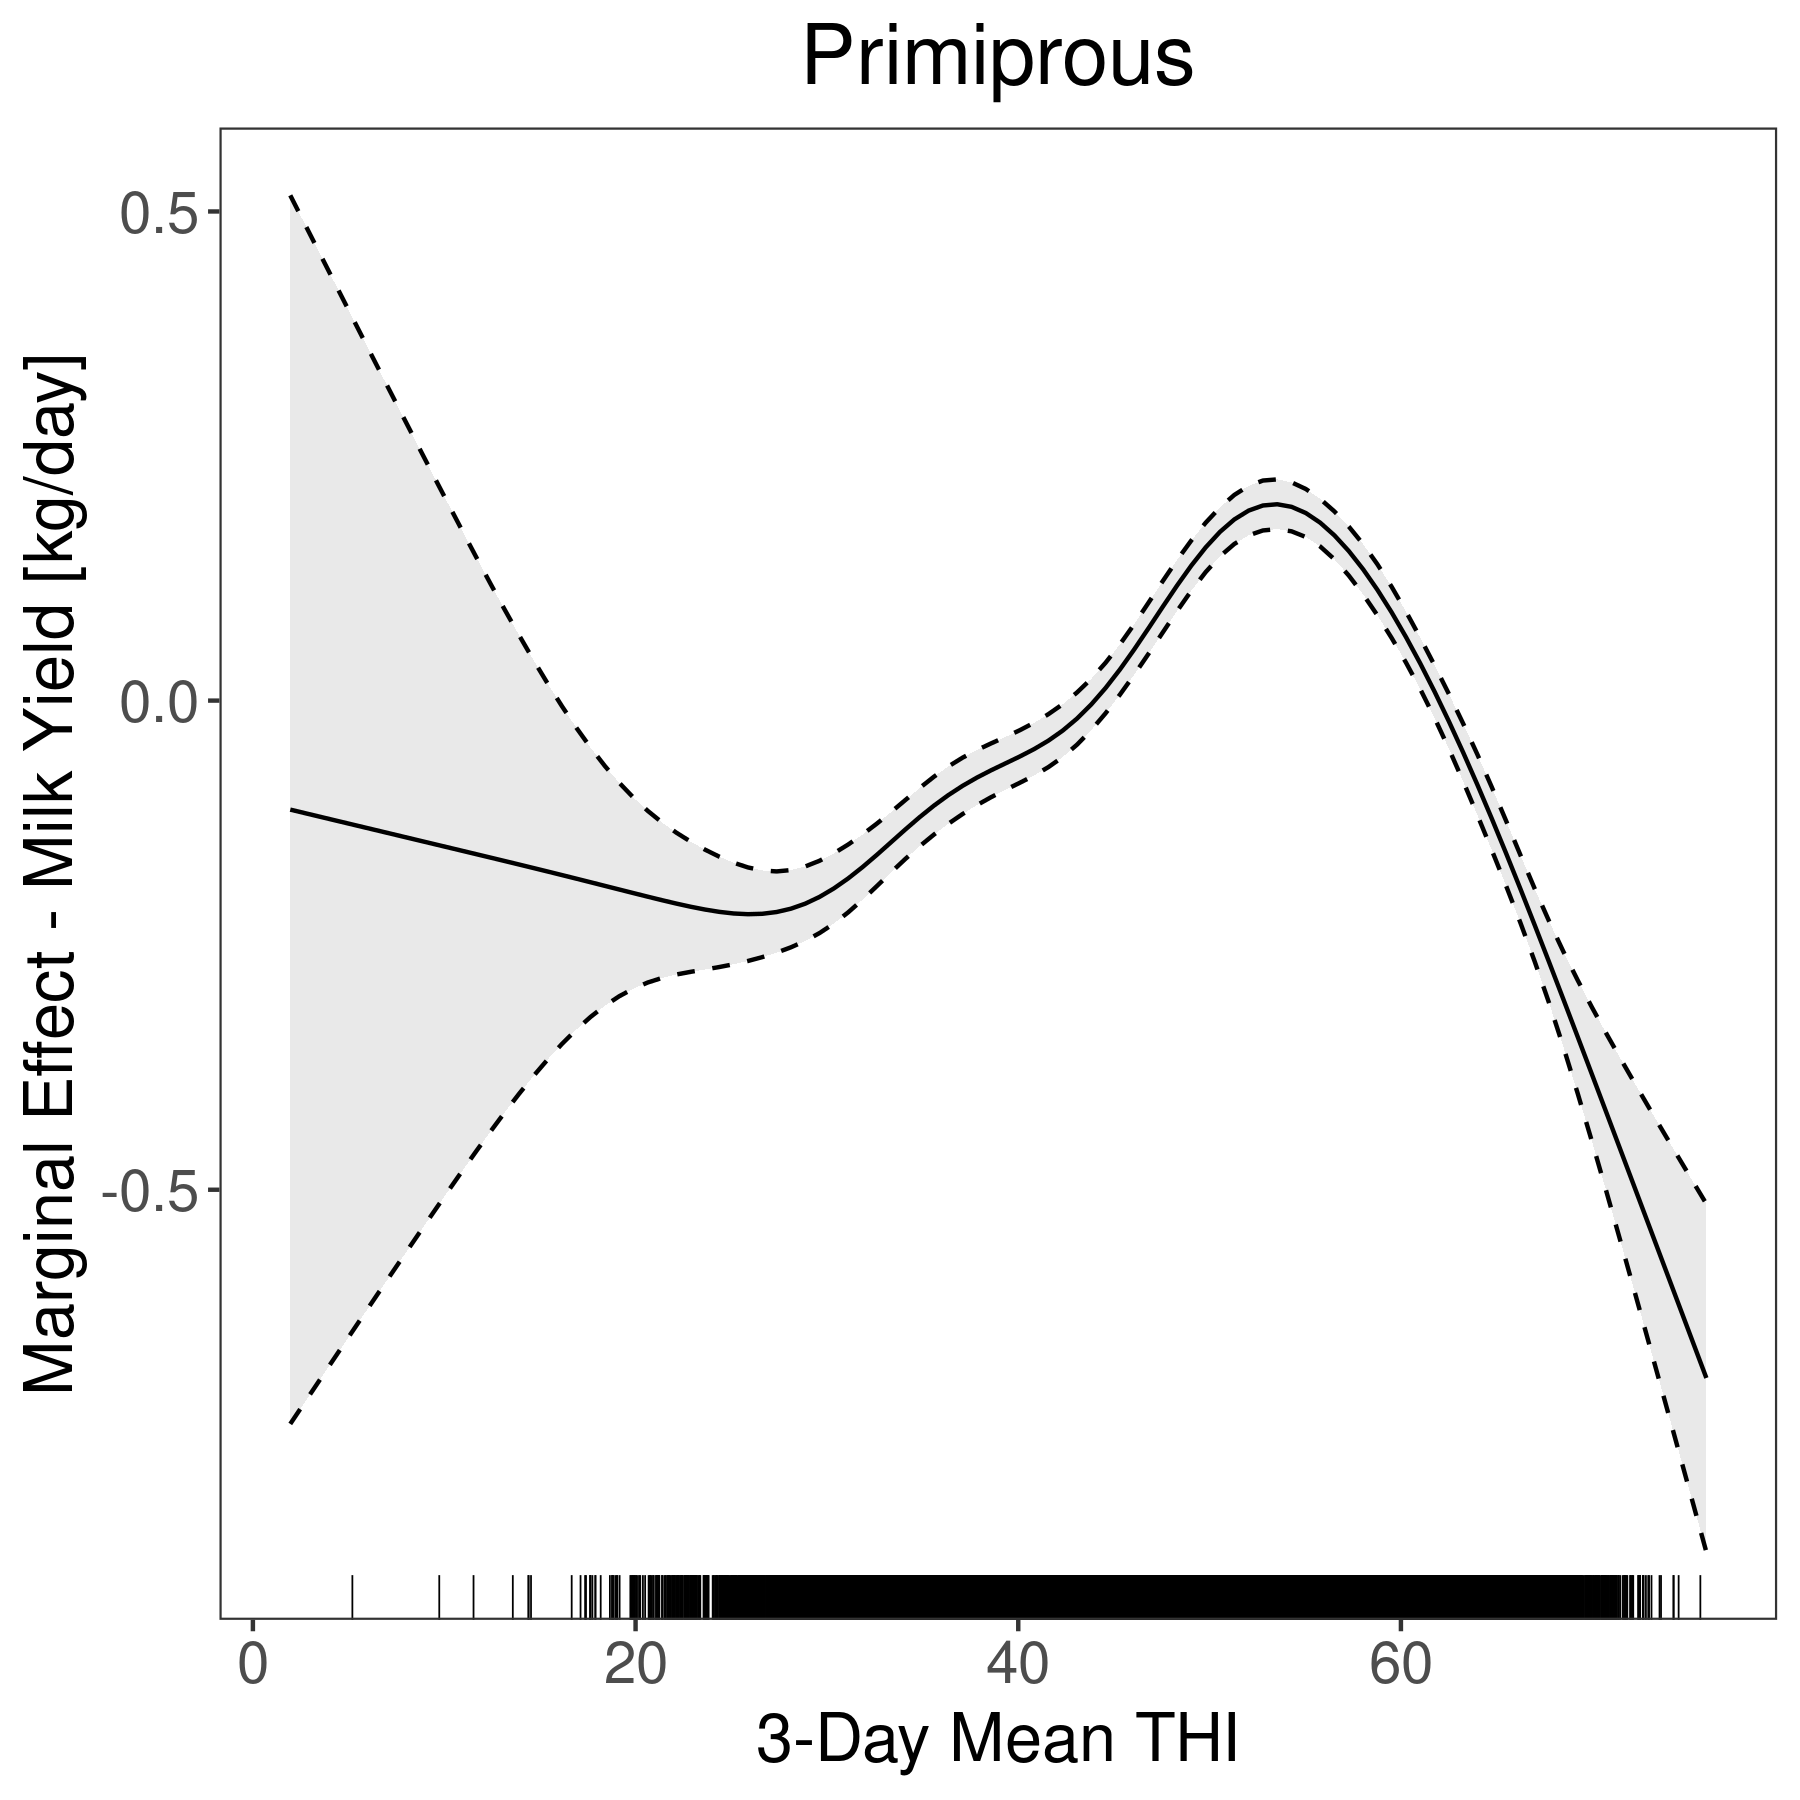
\includegraphics[width=\textwidth]{thesis/figures/models/milk/before2010/ho_milk_before2010/ho_milk_before2010_marginal_thi_milk_primi.png}
    \end{subfigure}
    \hspace{0.05\textwidth} % Optional space between the figures
    \begin{subfigure}[b]{0.45\textwidth}
        \centering
        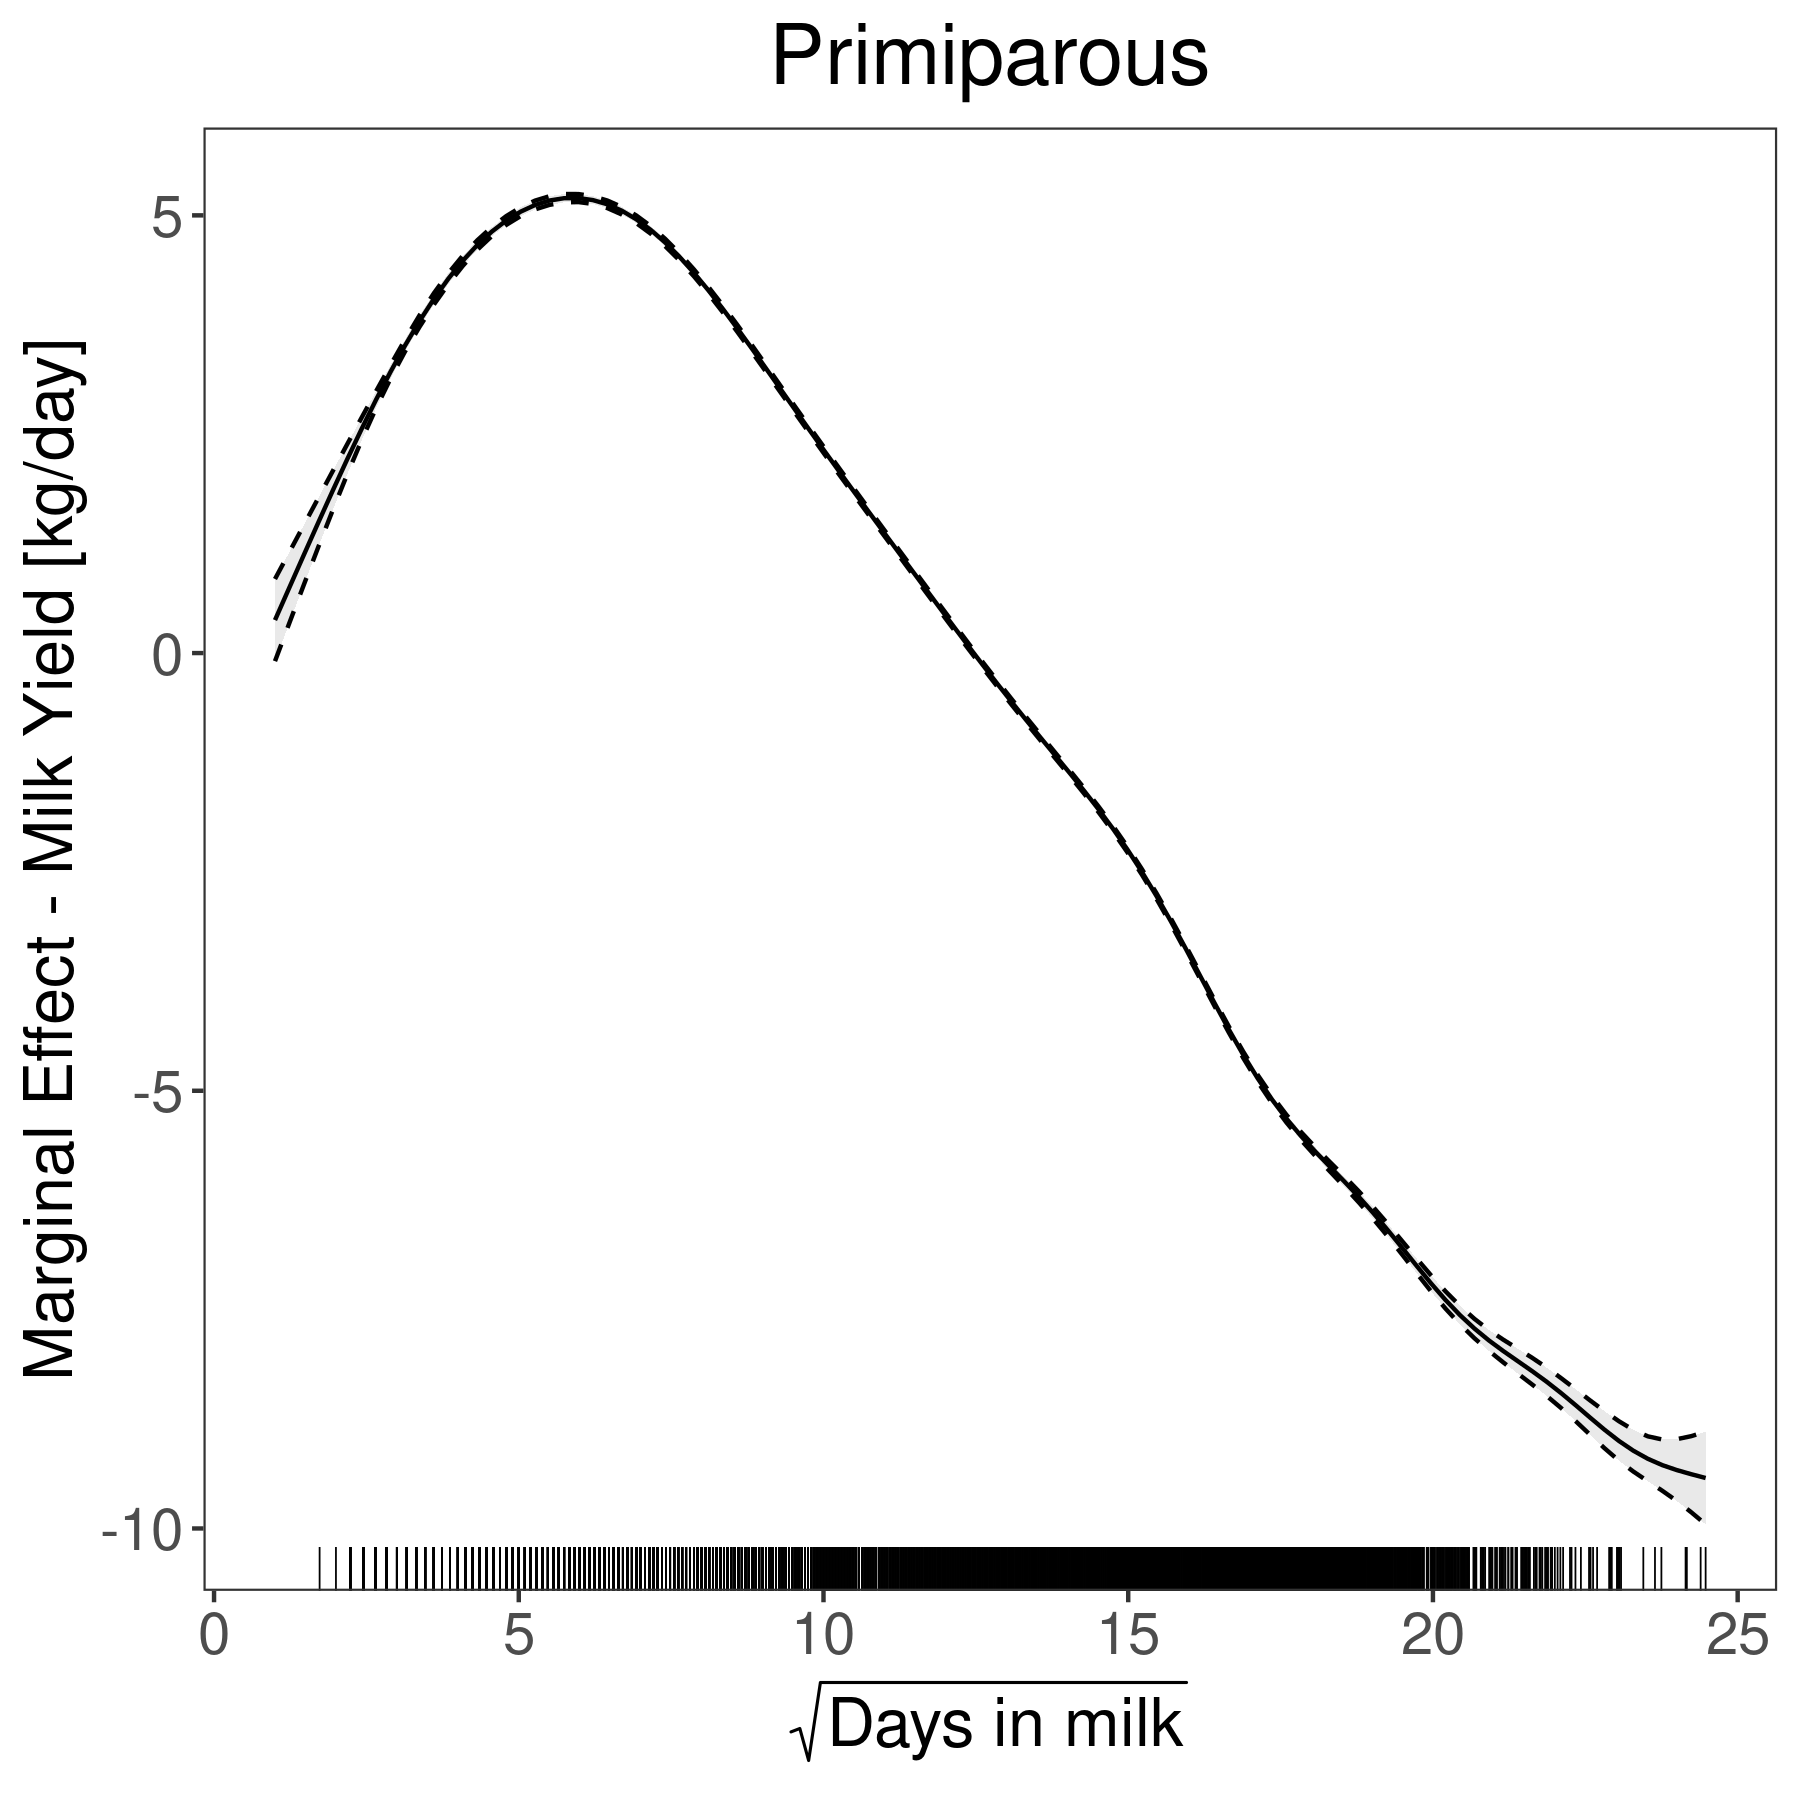
\includegraphics[width=\textwidth]{thesis/figures/models/milk/before2010/ho_milk_before2010/ho_milk_before2010_marginal_dim_milk_primi.png}
    \end{subfigure}
    \begin{subfigure}[b]{0.45\textwidth}
        \centering
        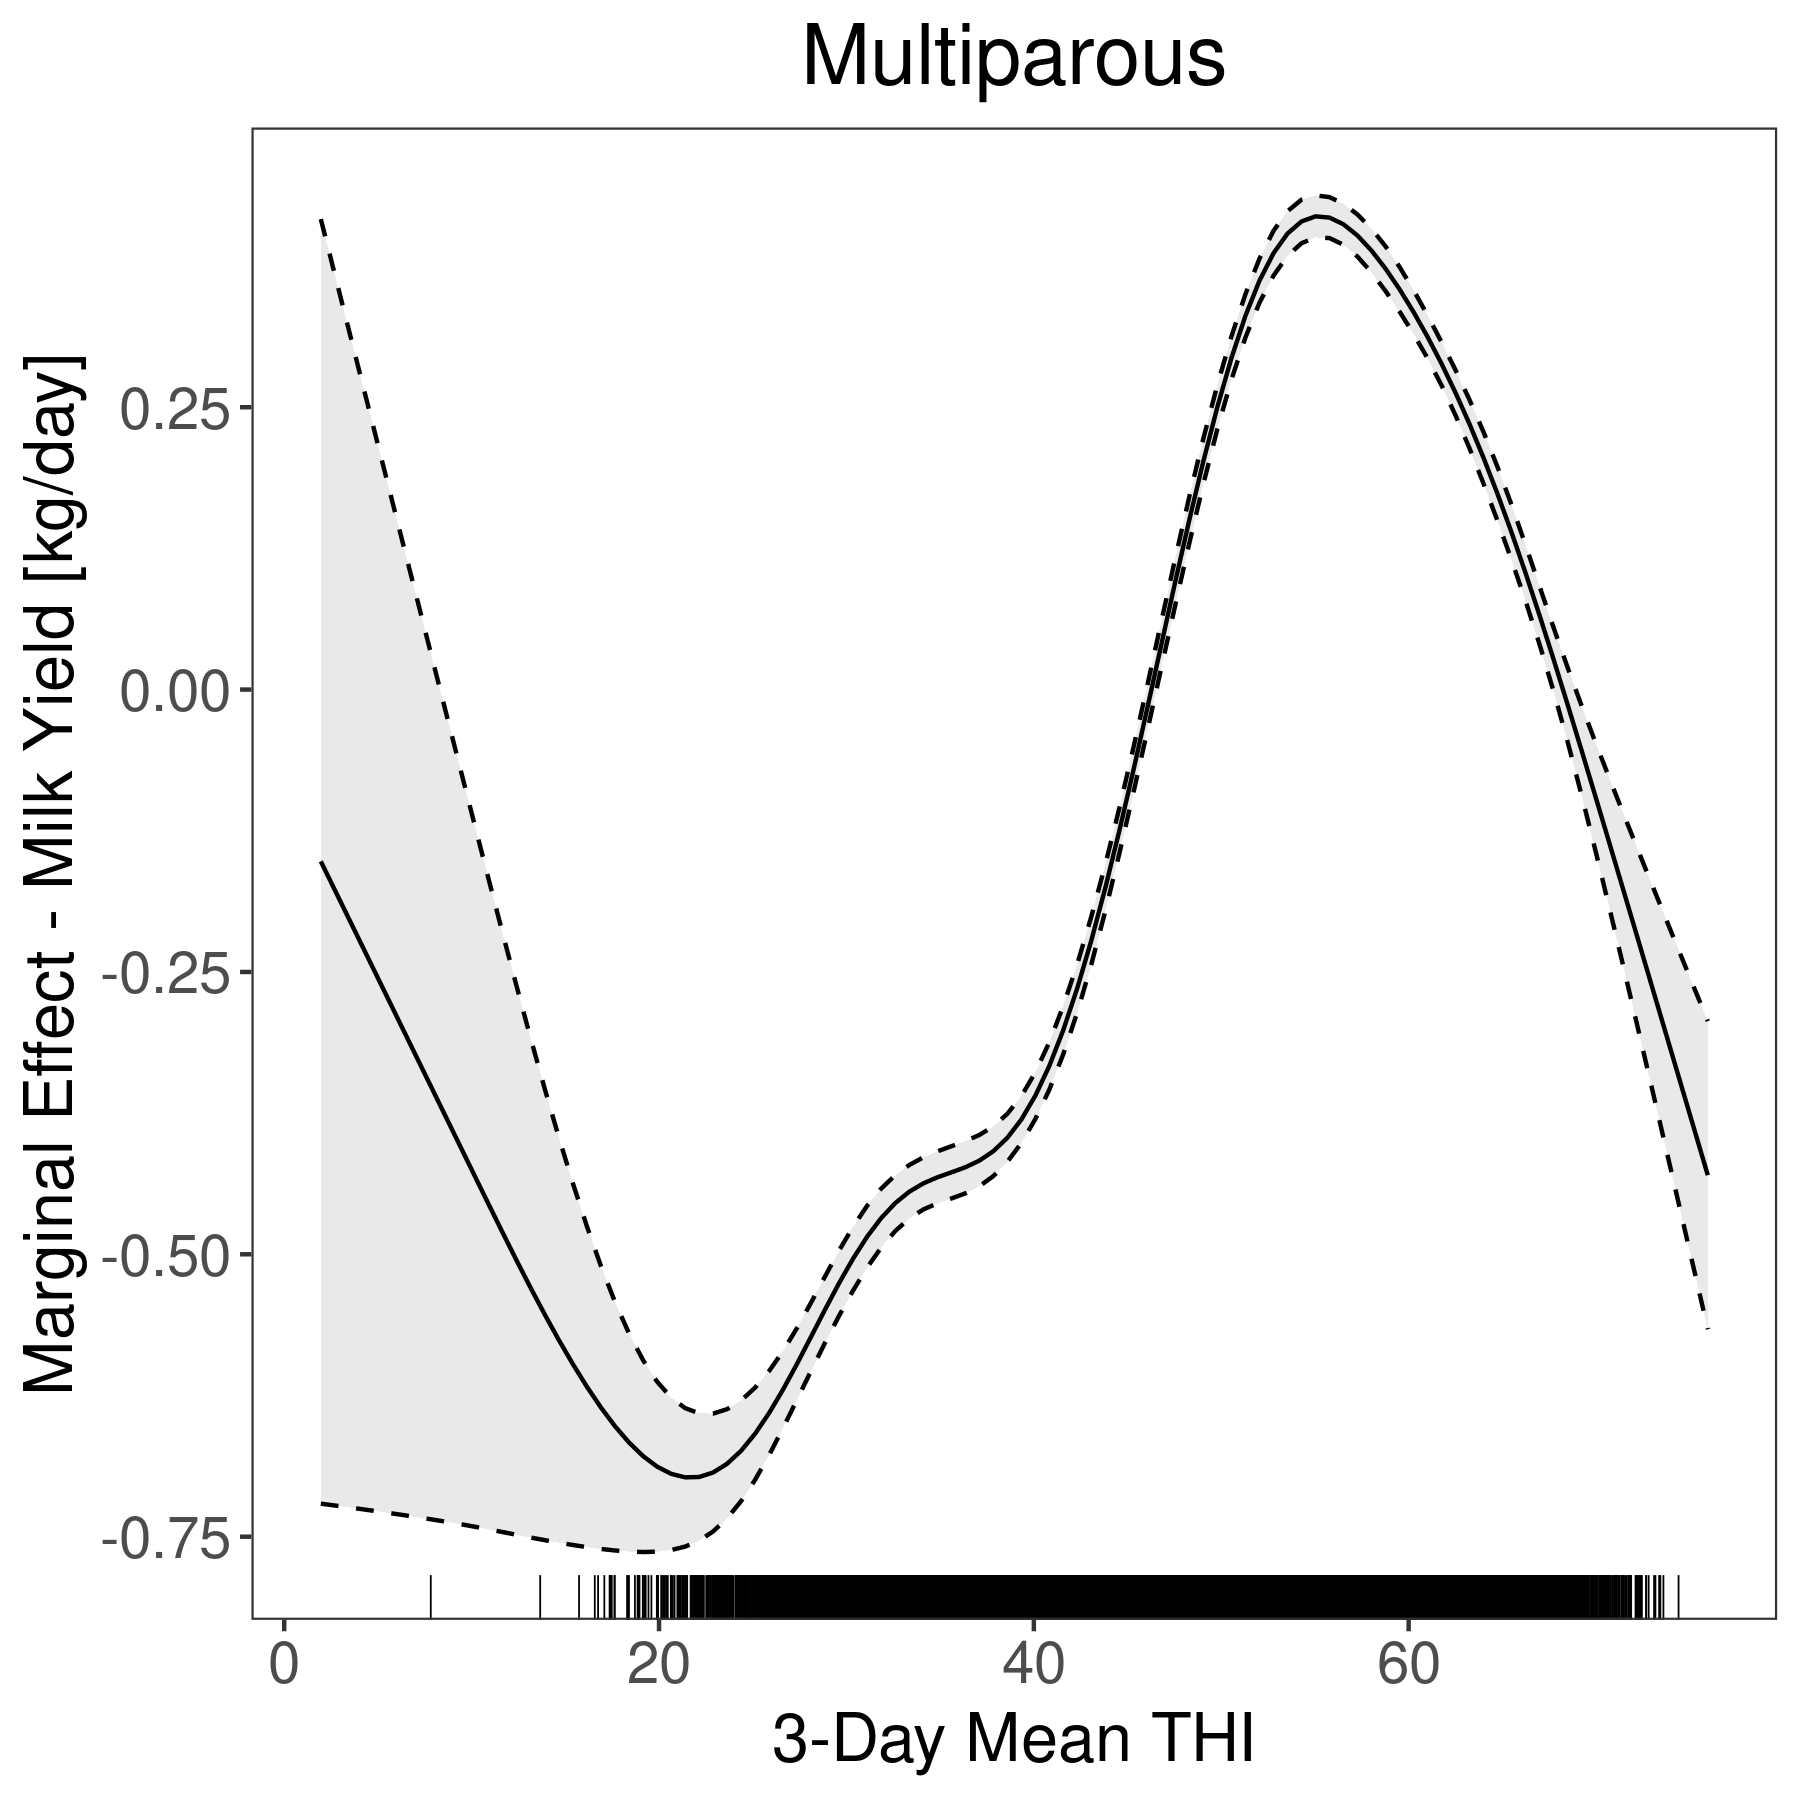
\includegraphics[width=\textwidth]{thesis/figures/models/milk/before2010/ho_milk_before2010/ho_milk_before2010_marginal_thi_milk_multi.png}
    \end{subfigure}
    \hspace{0.05\textwidth} % Optional space between the figures
    \begin{subfigure}[b]{0.45\textwidth}
        \centering
        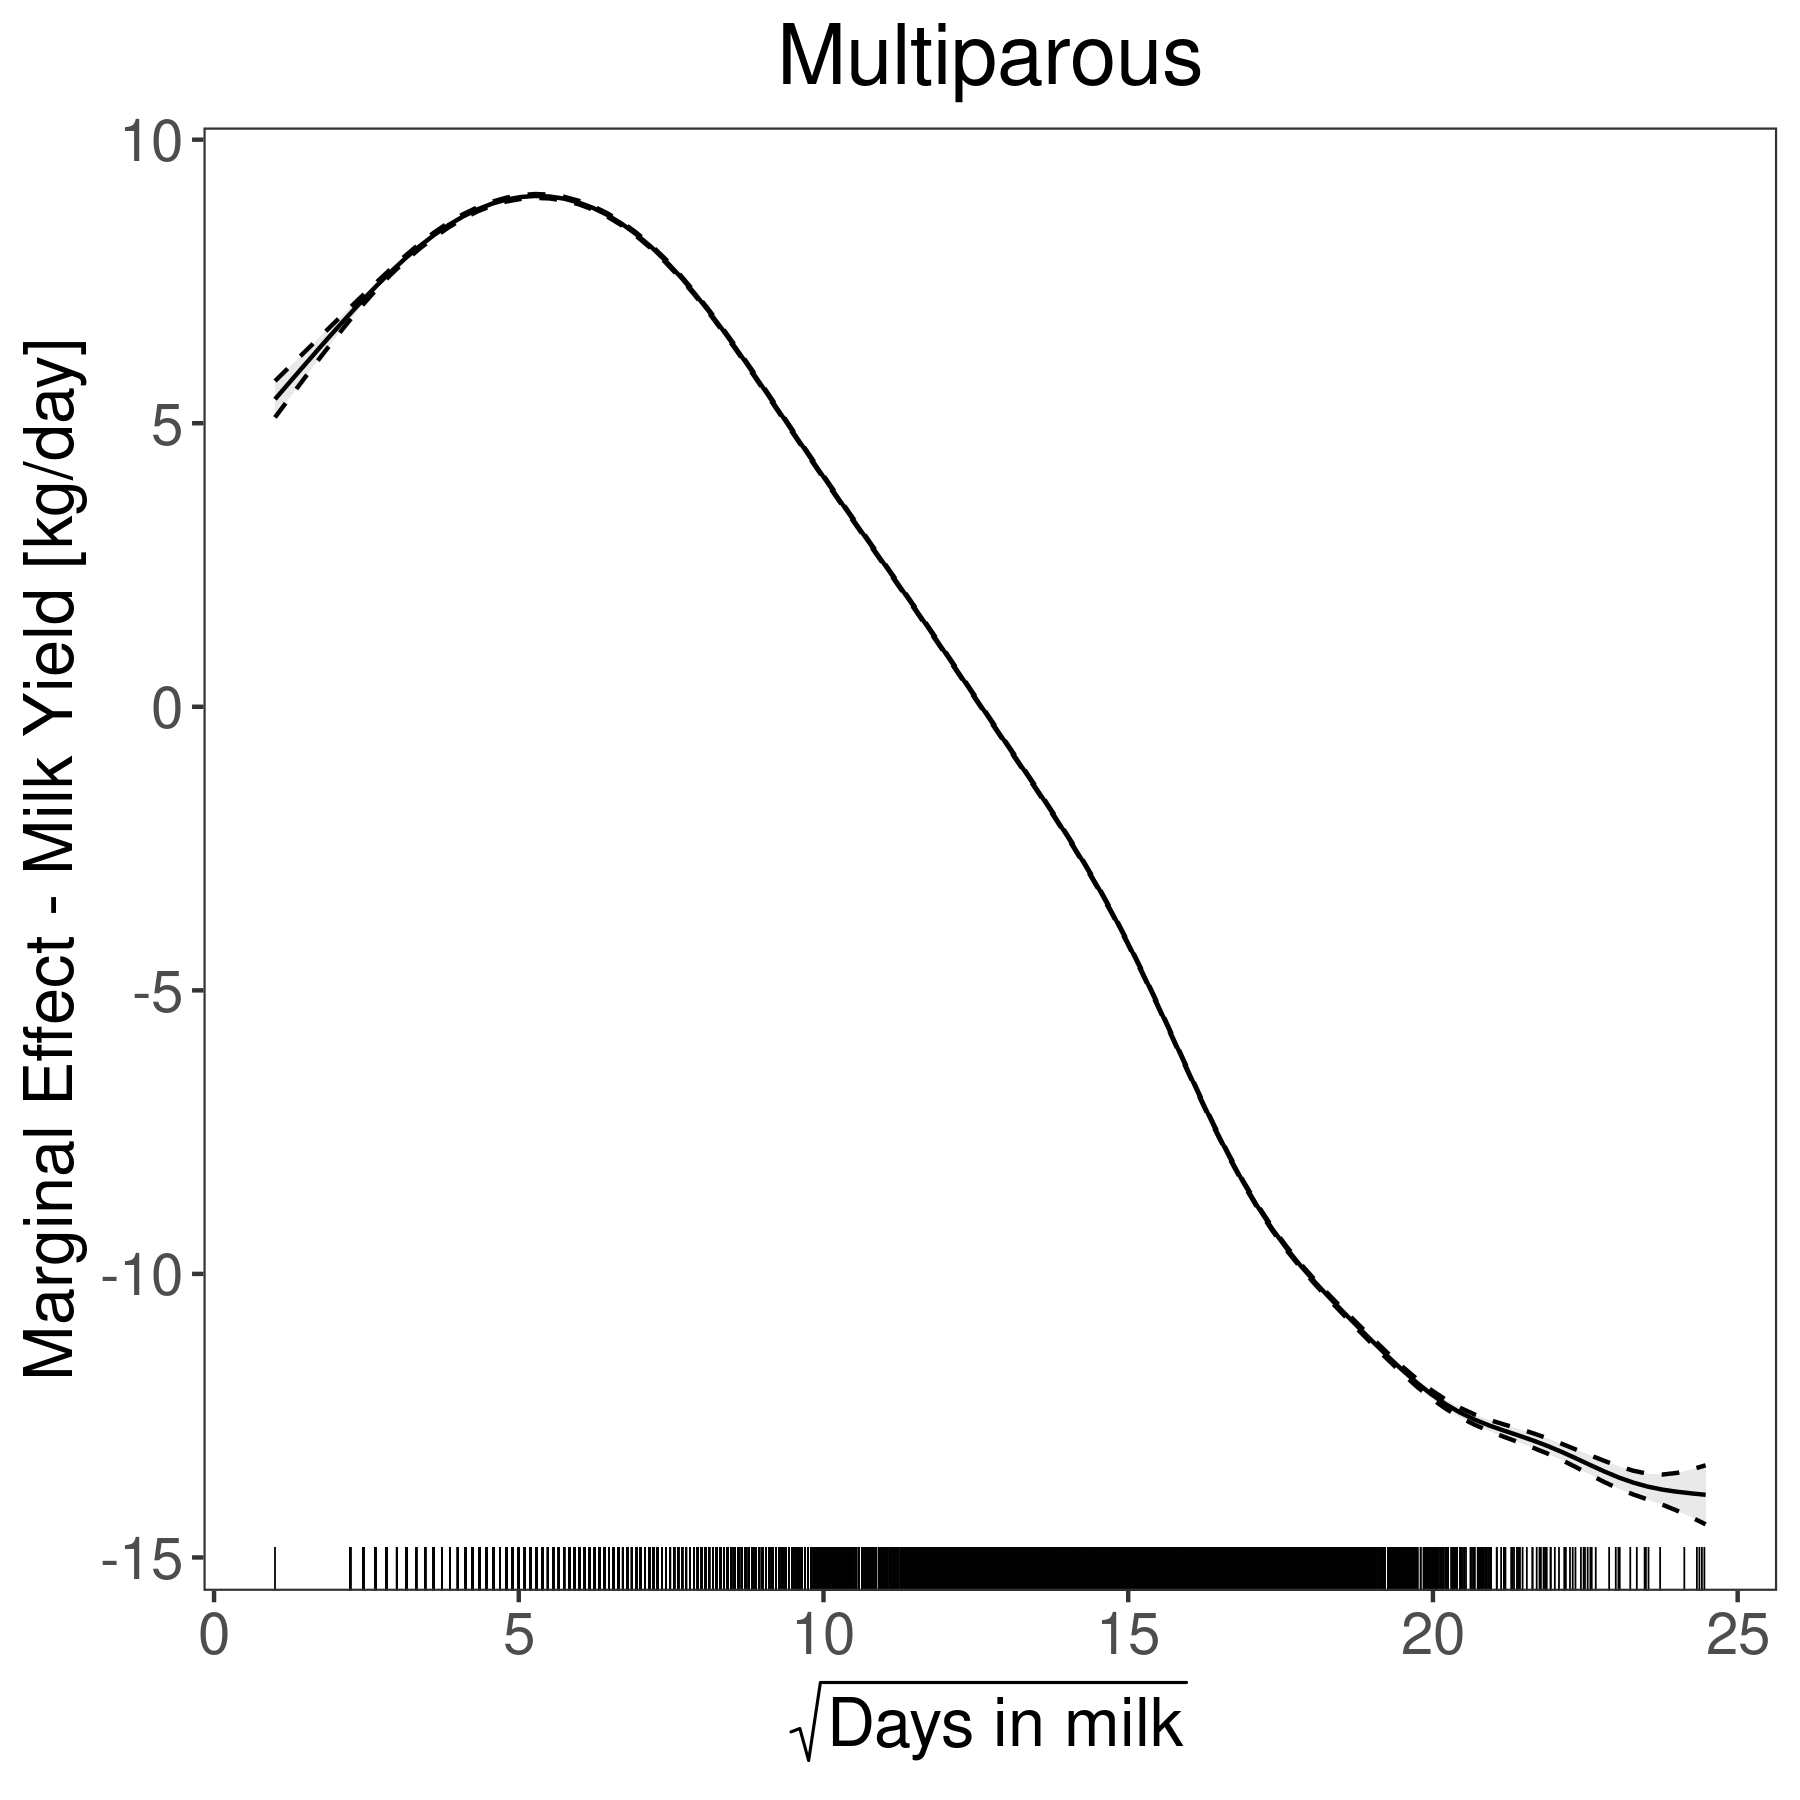
\includegraphics[width=\textwidth]{thesis/figures/models/milk/before2010/ho_milk_before2010/ho_milk_before2010_marginal_dim_milk_multi.png}
    \end{subfigure}
    \caption[]{Holstein: Milk Yield - 1985 - 2010 - THI Effect and Lactation Curve}
    \label{fig:main}
\end{figure}

\subsubsection{Split Period: 2010 - 2023}\label{model:ho_milk_after}

\paragraph{Model Summary} \quad \\

    \begin{table}[H]
    \centering
    \begin{tabular}{lrrrr}
    \textbf{A. parametric coefficients} & Estimate & Std. Error & t-value & p-value \\ 
       \hline
       \hline
  (Intercept) & 23.8289 & 0.3841 & 62.0385 & $<$ 0.0001 \\ 
  parityprimiparous & -3.5815 & 0.0143 & -250.7346 & $<$ 0.0001 \\ 
  year2012 & -0.1435 & 0.4281 & -0.3352 & 0.7375 \\ 
  year2013 & -0.4446 & 0.4293 & -1.0358 & 0.3003 \\ 
  year2014 & 0.1502 & 0.4291 & 0.3501 & 0.7263 \\ 
  year2015 & 0.4723 & 0.4308 & 1.0965 & 0.2728 \\ 
  year2016 & 0.7635 & 0.4567 & 1.6718 & 0.0946 \\ 
  year2017 & 1.1762 & 0.4488 & 2.6207 & 0.0088 \\ 
  year2018 & 1.7098 & 0.4437 & 3.8535 & 0.0001 \\ 
  year2019 & 1.9267 & 0.4429 & 4.3500 & $<$ 0.0001 \\ 
  year2020 & 2.4354 & 0.4451 & 5.4719 & $<$ 0.0001 \\ 
  year2021 & 2.6773 & 0.4567 & 5.8617 & $<$ 0.0001 \\ 
  year2022 & 2.5650 & 0.4533 & 5.6584 & $<$ 0.0001 \\ 
  year2023 & 2.9380 & 0.4808 & 6.1102 & $<$ 0.0001 \\ 
       \hline
    \textbf{B. smooth terms} & edf & Ref.df & F-value & p-value \\ 
    \hline
    \hline
  s(thi\_mean\_t0\_3d):paritymultiparous & 8.3215 & 8.3215 & 484.5057 & $<$ 0.0001 \\ 
  s(thi\_mean\_t0\_3d):parityprimiparous & 7.0657 & 7.0657 & 29.5389 & $<$ 0.0001 \\ 
  s(days\_in\_milk\_t):paritymultiparous & 14.6827 & 14.6827 & 114849.4858 & $<$ 0.0001 \\ 
  s(days\_in\_milk\_t):parityprimiparous & 13.9847 & 13.9847 & 12129.3973 & $<$ 0.0001 \\ 
       \hline
    \end{tabular}
    \caption[]{Holstein: Milk Yield - 2011-2023 - GAMM model summary without random effect terms.}
    \end{table}

\newpage
\begin{table}[H]
\centering
\begin{tabular}
{l | r | r | r | r}
\textbf{Smooth Term Fixed Effect} & Est. & SE & z & p\\
\hline
\hline
s(thi\_mean\_t0\_3d):multiFx1 & -0.5663 & 0.1050 & -5.39 & $<$ 1e-07\\
s(thi\_mean\_t0\_3d):primiFx1 & -0.4351 & 0.1310 & -3.32 & 0.0009\\
s(days\_in\_milk\_):multiFx1 & 6.2500 & 0.5244 & 11.92 & $<$ 1e-32\\
s(days\_in\_milk\_):primiFx1 &  3.9576 & 0.6407 & 6.18 & $<$ 1e-09\\
\hline
\textbf{Variance Component} & Estimated $\sigma$ & & & \\
\hline
\hline
$\sigma_\alpha$ & 3.1563 & &  & \\
$\sigma_\iota$ & 1.1935 & & & \\
$\sigma_\phi$ & 3.7462 & & & \\
s(thi\_mean\_t0\_3d):multi & 2.2598 & & & \\
s(days\_in\_milk\_):primi & 8.5279 & & & \\
s(days\_in\_milk\_):multi & 12.0097 & & & \\
s(thi\_mean\_t0\_3d):primi & 1.6772 & & & \\
Residual & 3.9639 & & & \\
\end{tabular}
\caption[]{Holstein: Milk Yield - 2011-2023 - Mixed Model Summary - Smooth Terms and Random Effects.}
\end{table}

\paragraph{Model Diagnostics} \quad \\
\begin{figure}[H]
    \centering
    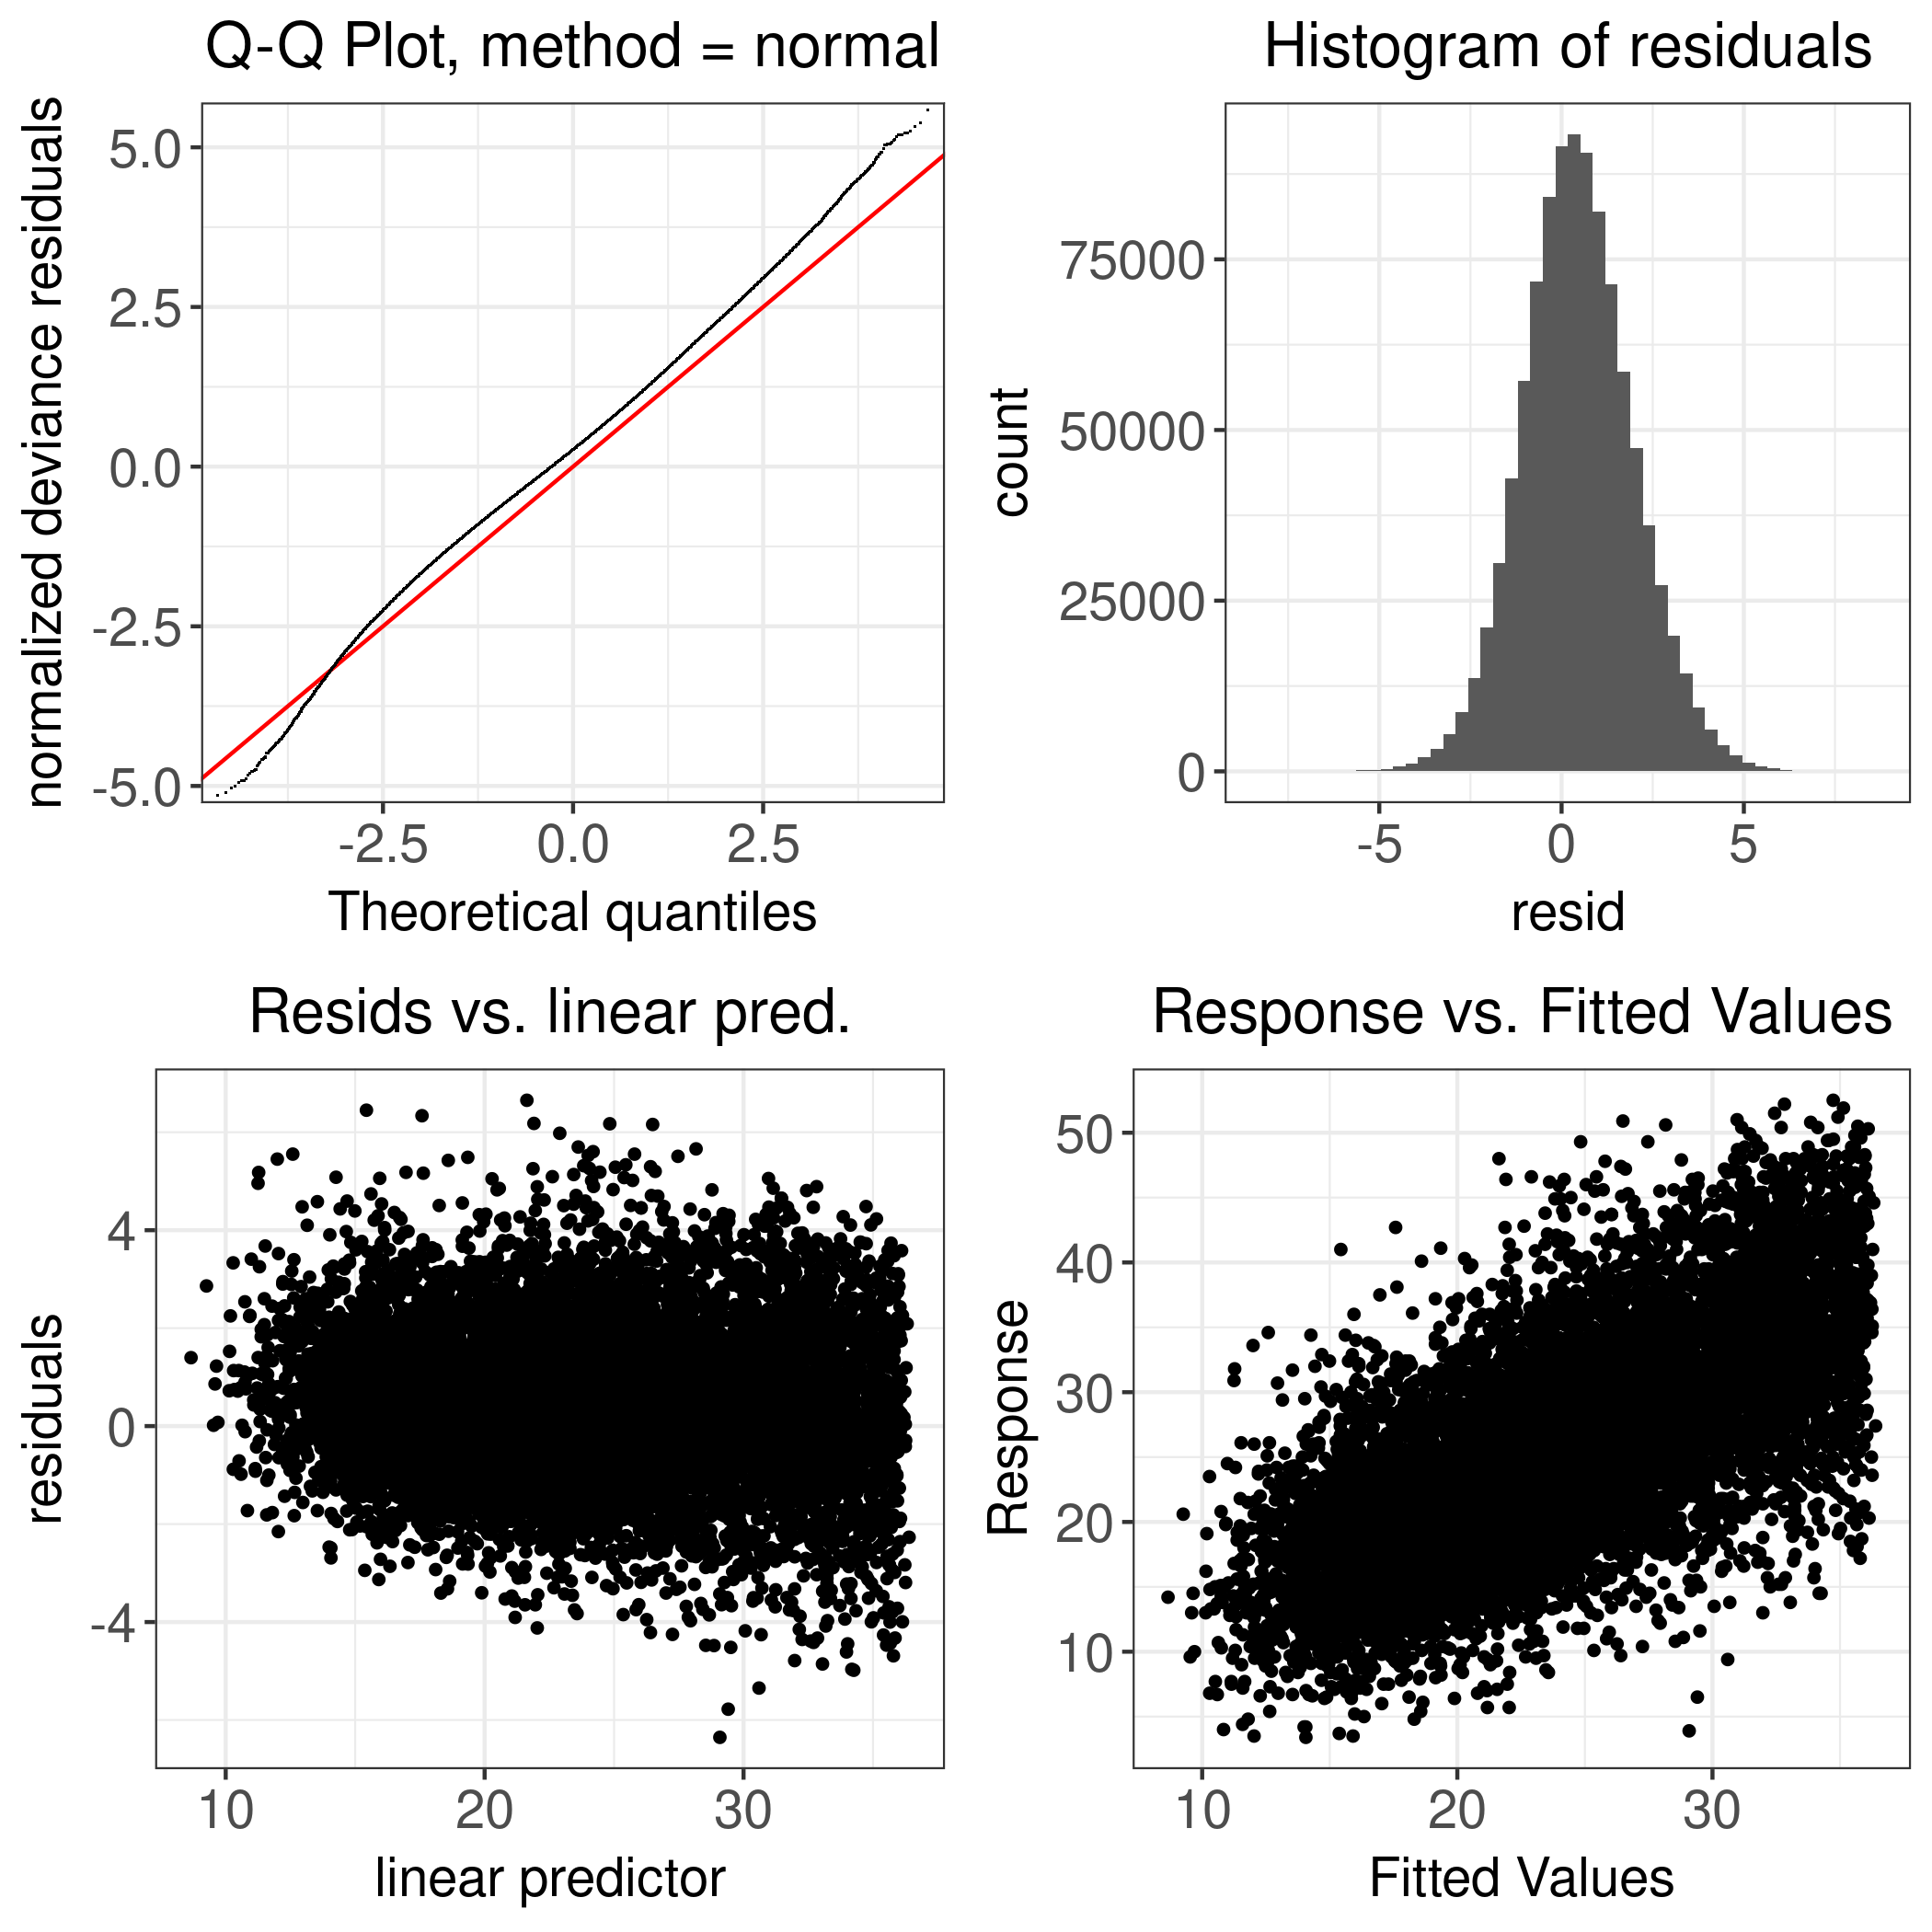
\includegraphics[width=0.6\textwidth]{thesis/figures/models/milk/after2010/ho_milk_after2010/ho_milk_after2010_diagnostics.png}
    \caption[]{Holstein: Milk Yield - 2011-2023 - Diagnostic Plot}
\end{figure}

\newpage
\paragraph{THI Effect and Lactation Curve} \quad \\
\begin{figure}[H]
    \centering
    \begin{subfigure}[b]{0.45\textwidth}
        \centering
        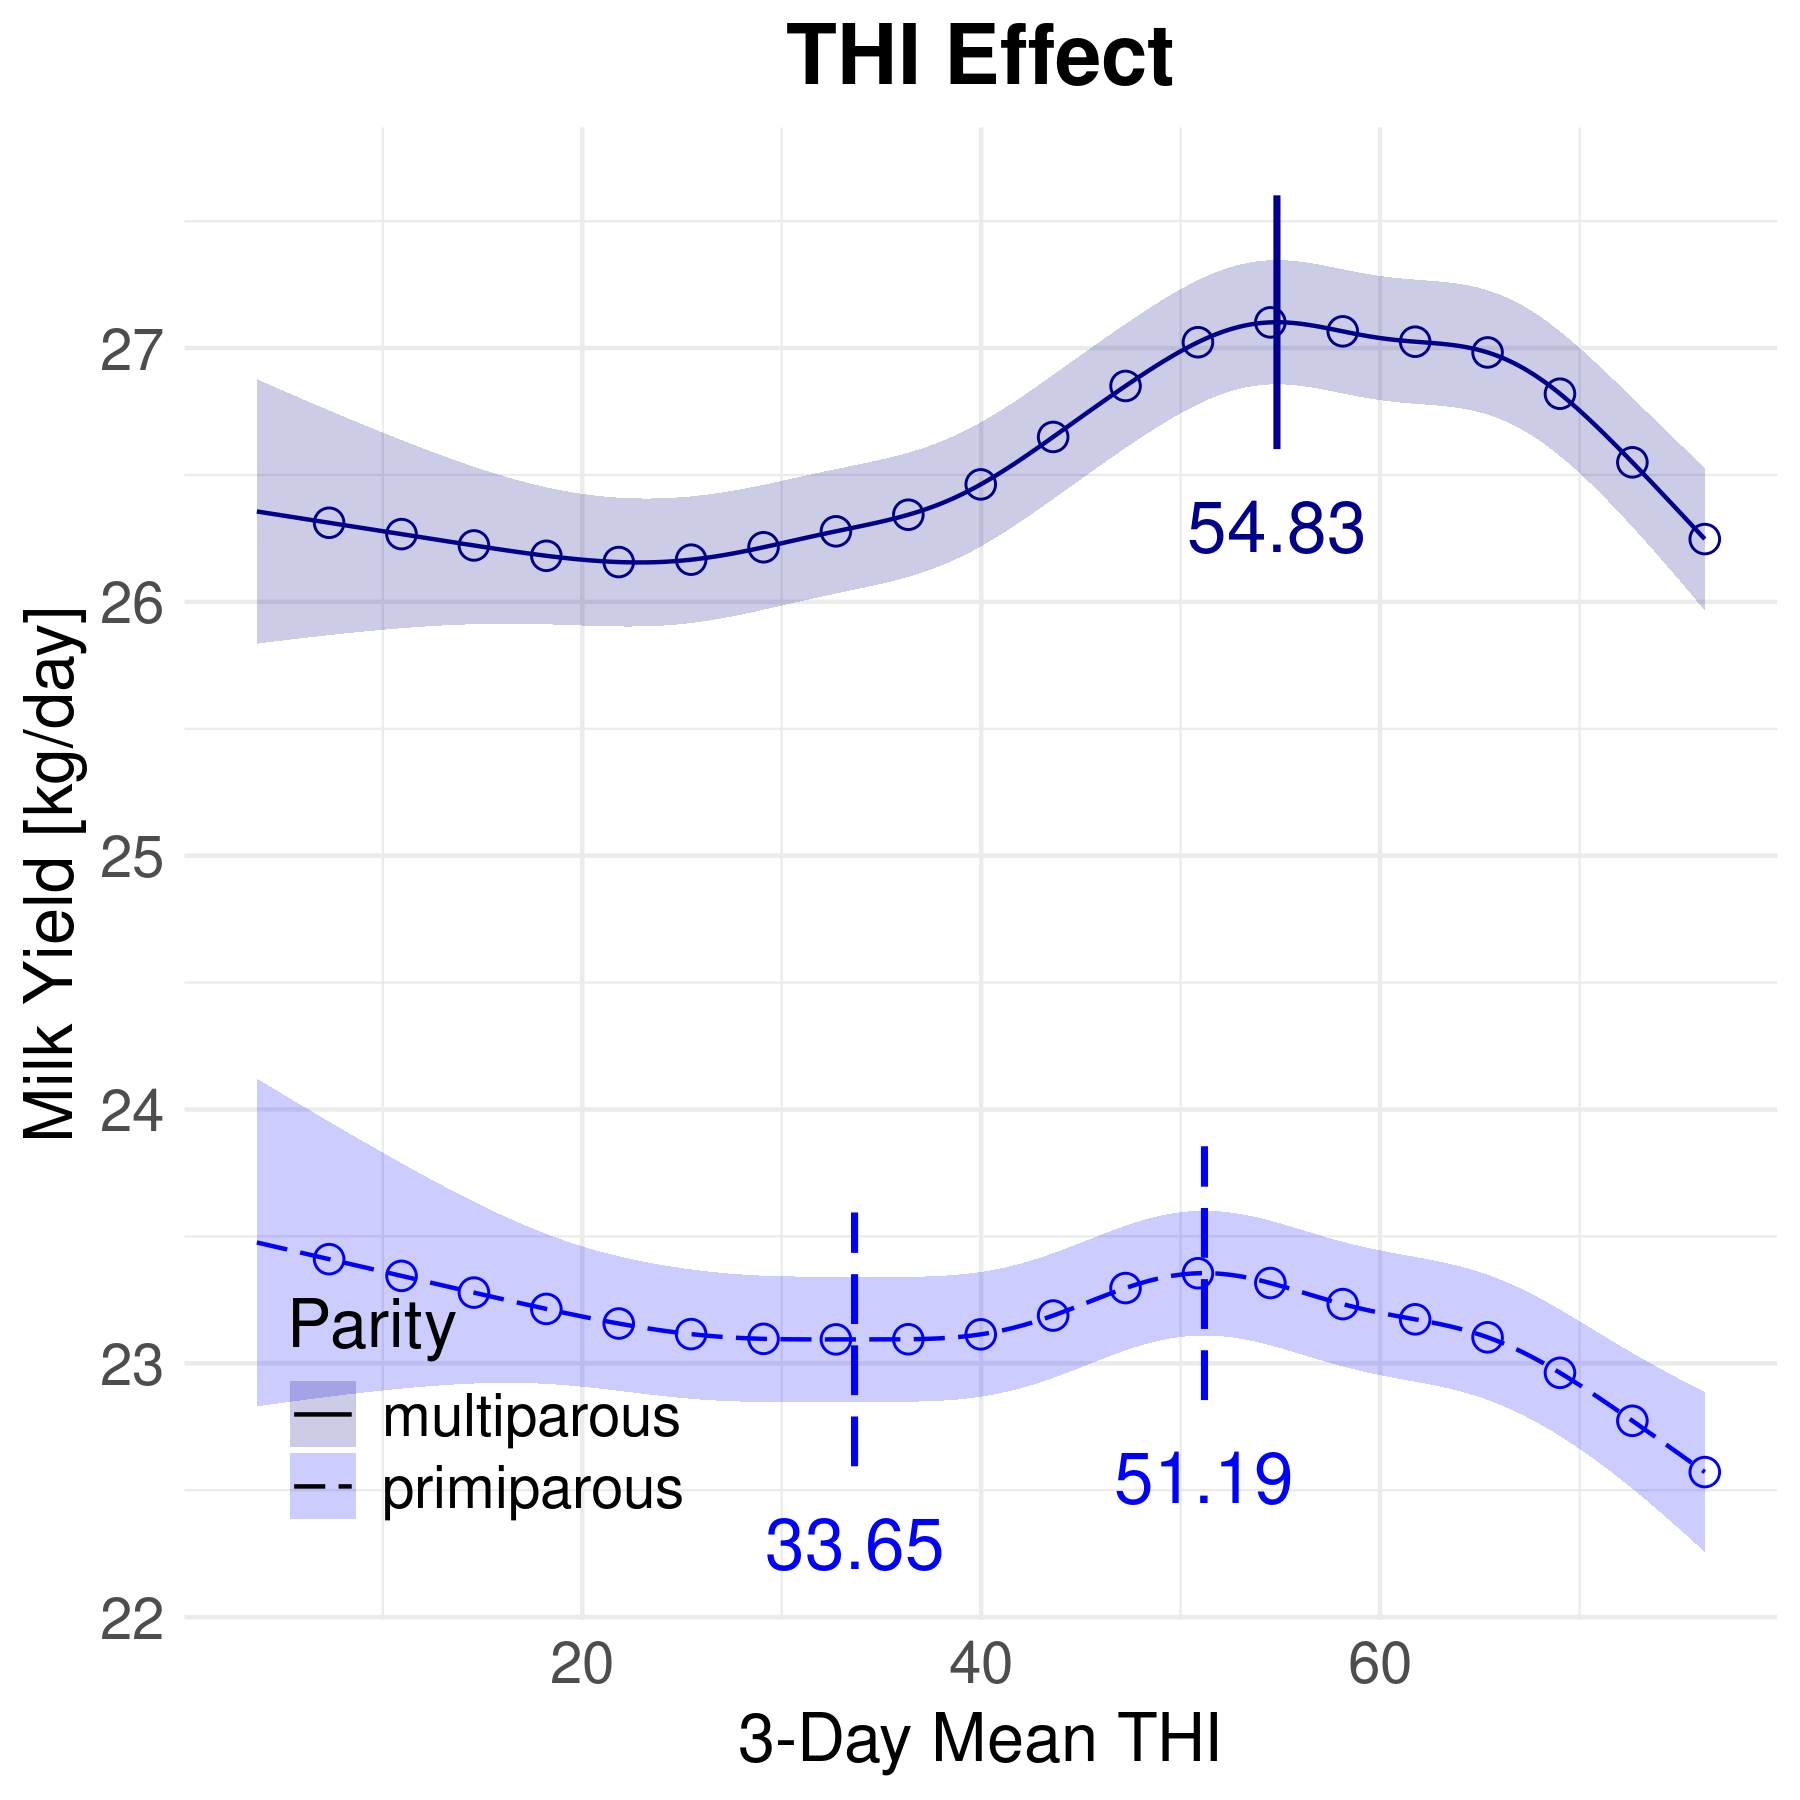
\includegraphics[width=\textwidth]{thesis/figures/models/milk/after2010/ho_milk_after2010/ho_milk_after2010_marginal_thi_milk_combined.png}
    \end{subfigure}
    \hspace{0.05\textwidth} % Optional space between the figures
    \begin{subfigure}[b]{0.45\textwidth}
        \centering
        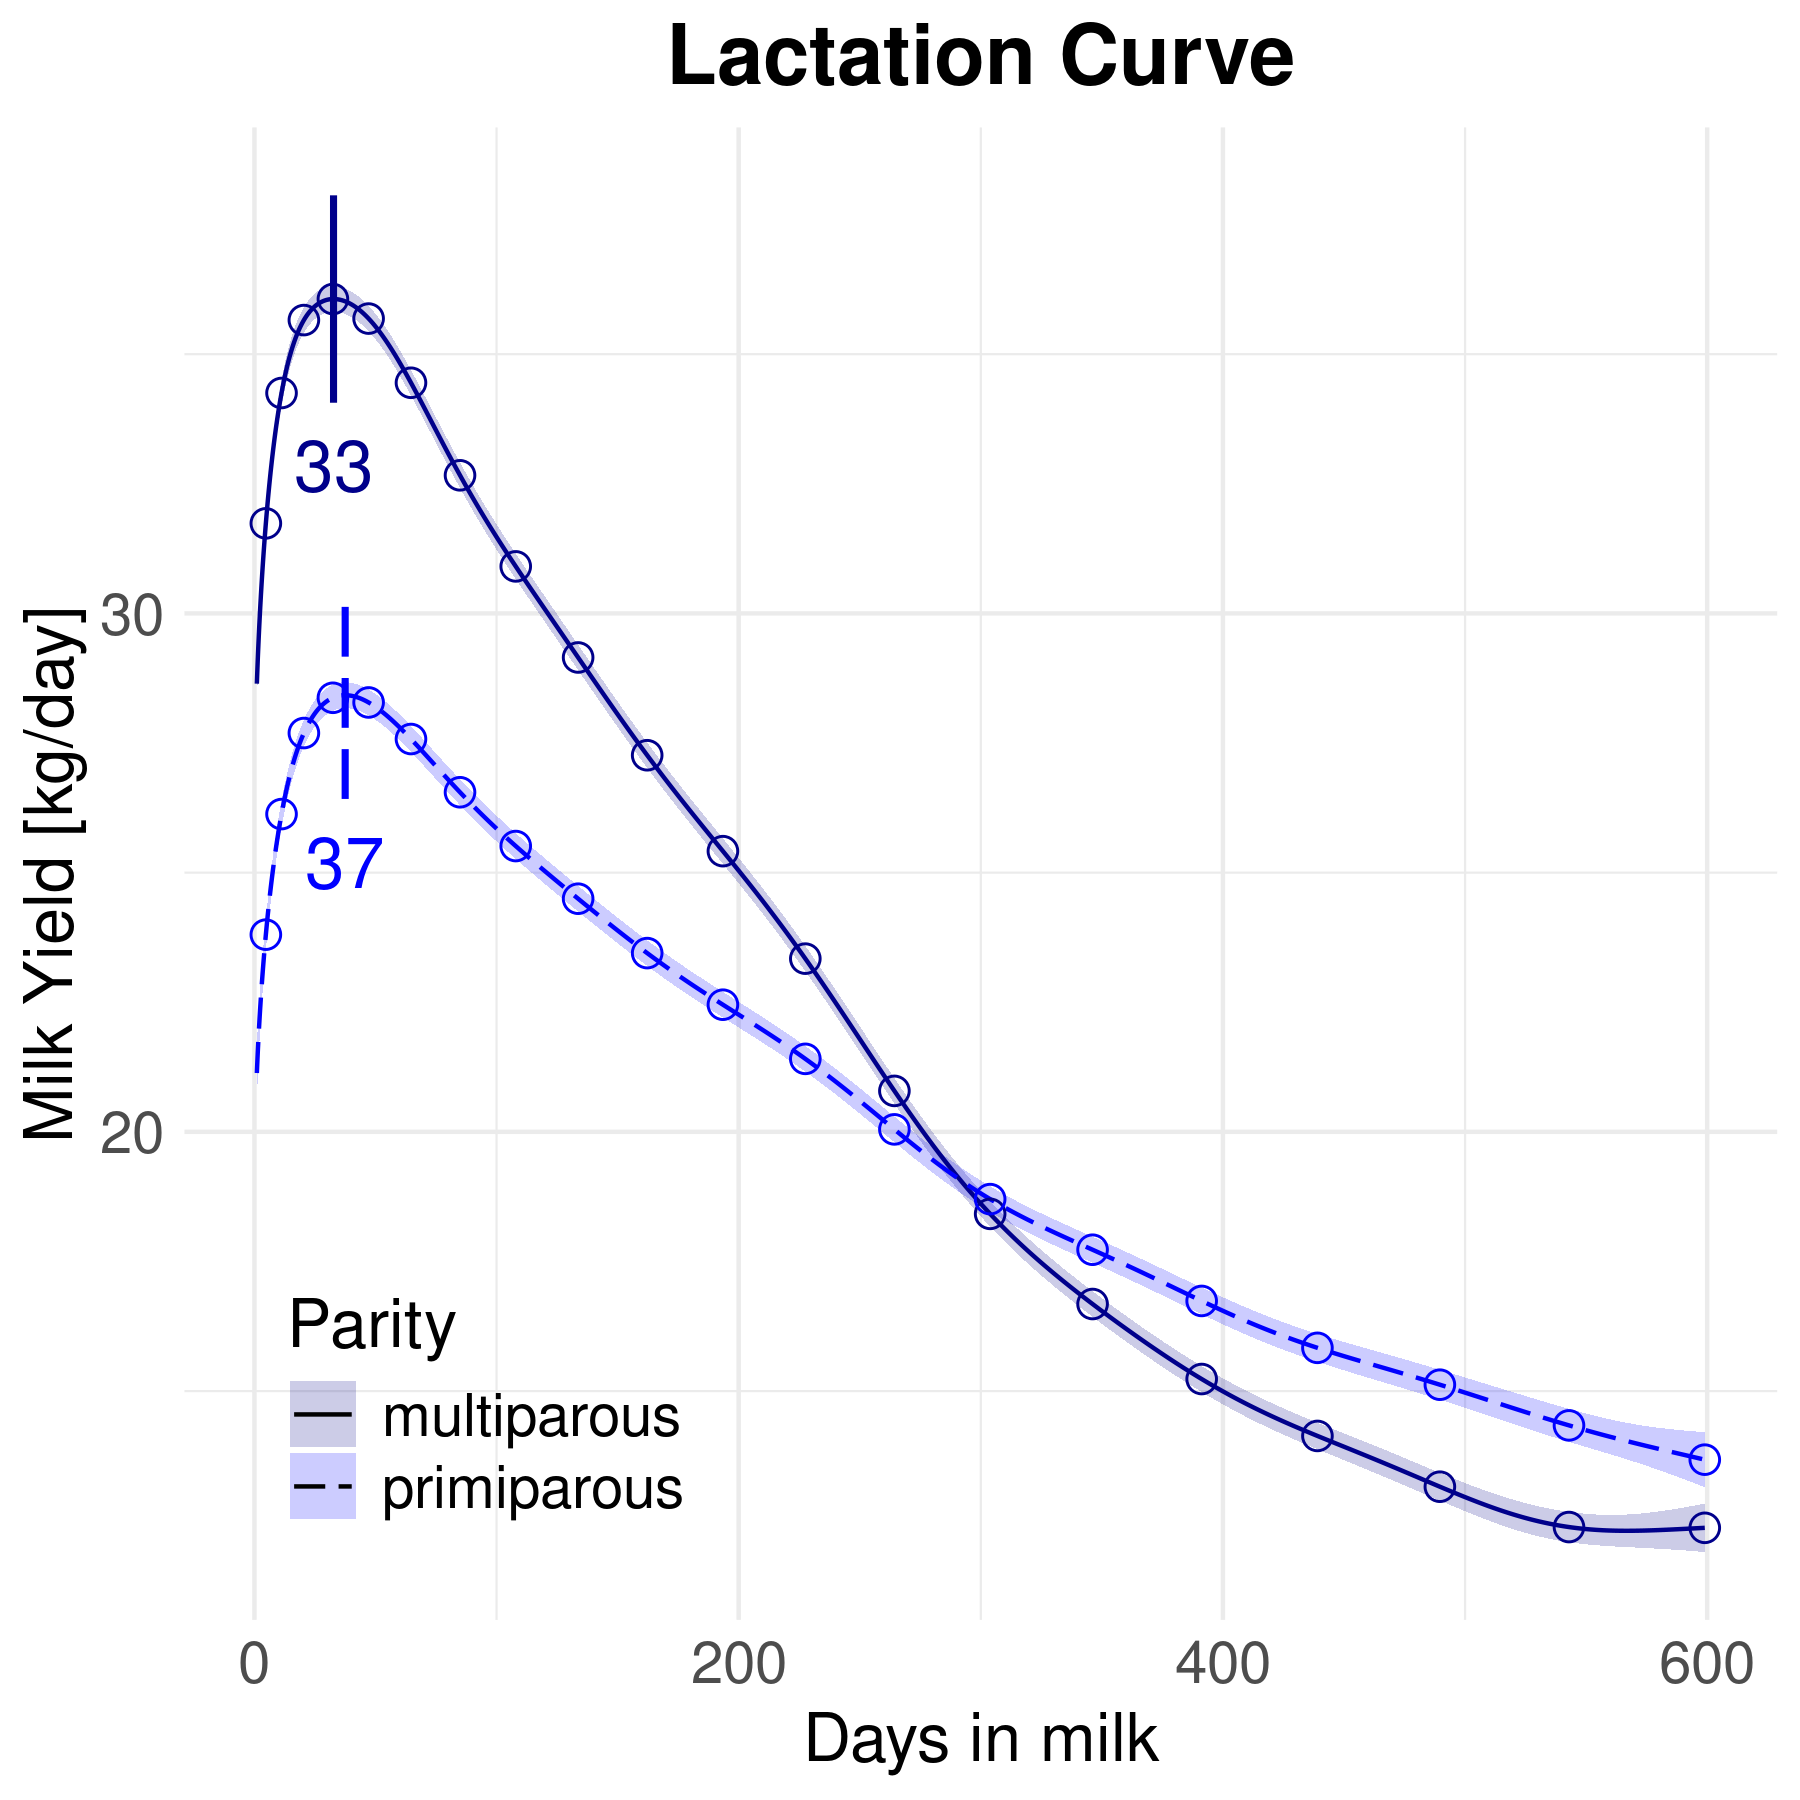
\includegraphics[width=\textwidth]{thesis/figures/models/milk/after2010/ho_milk_after2010/ho_milk_after2010_marginal_dim_milk_combined.png}
    \end{subfigure}
    \begin{subfigure}[b]{0.45\textwidth}
        \centering
        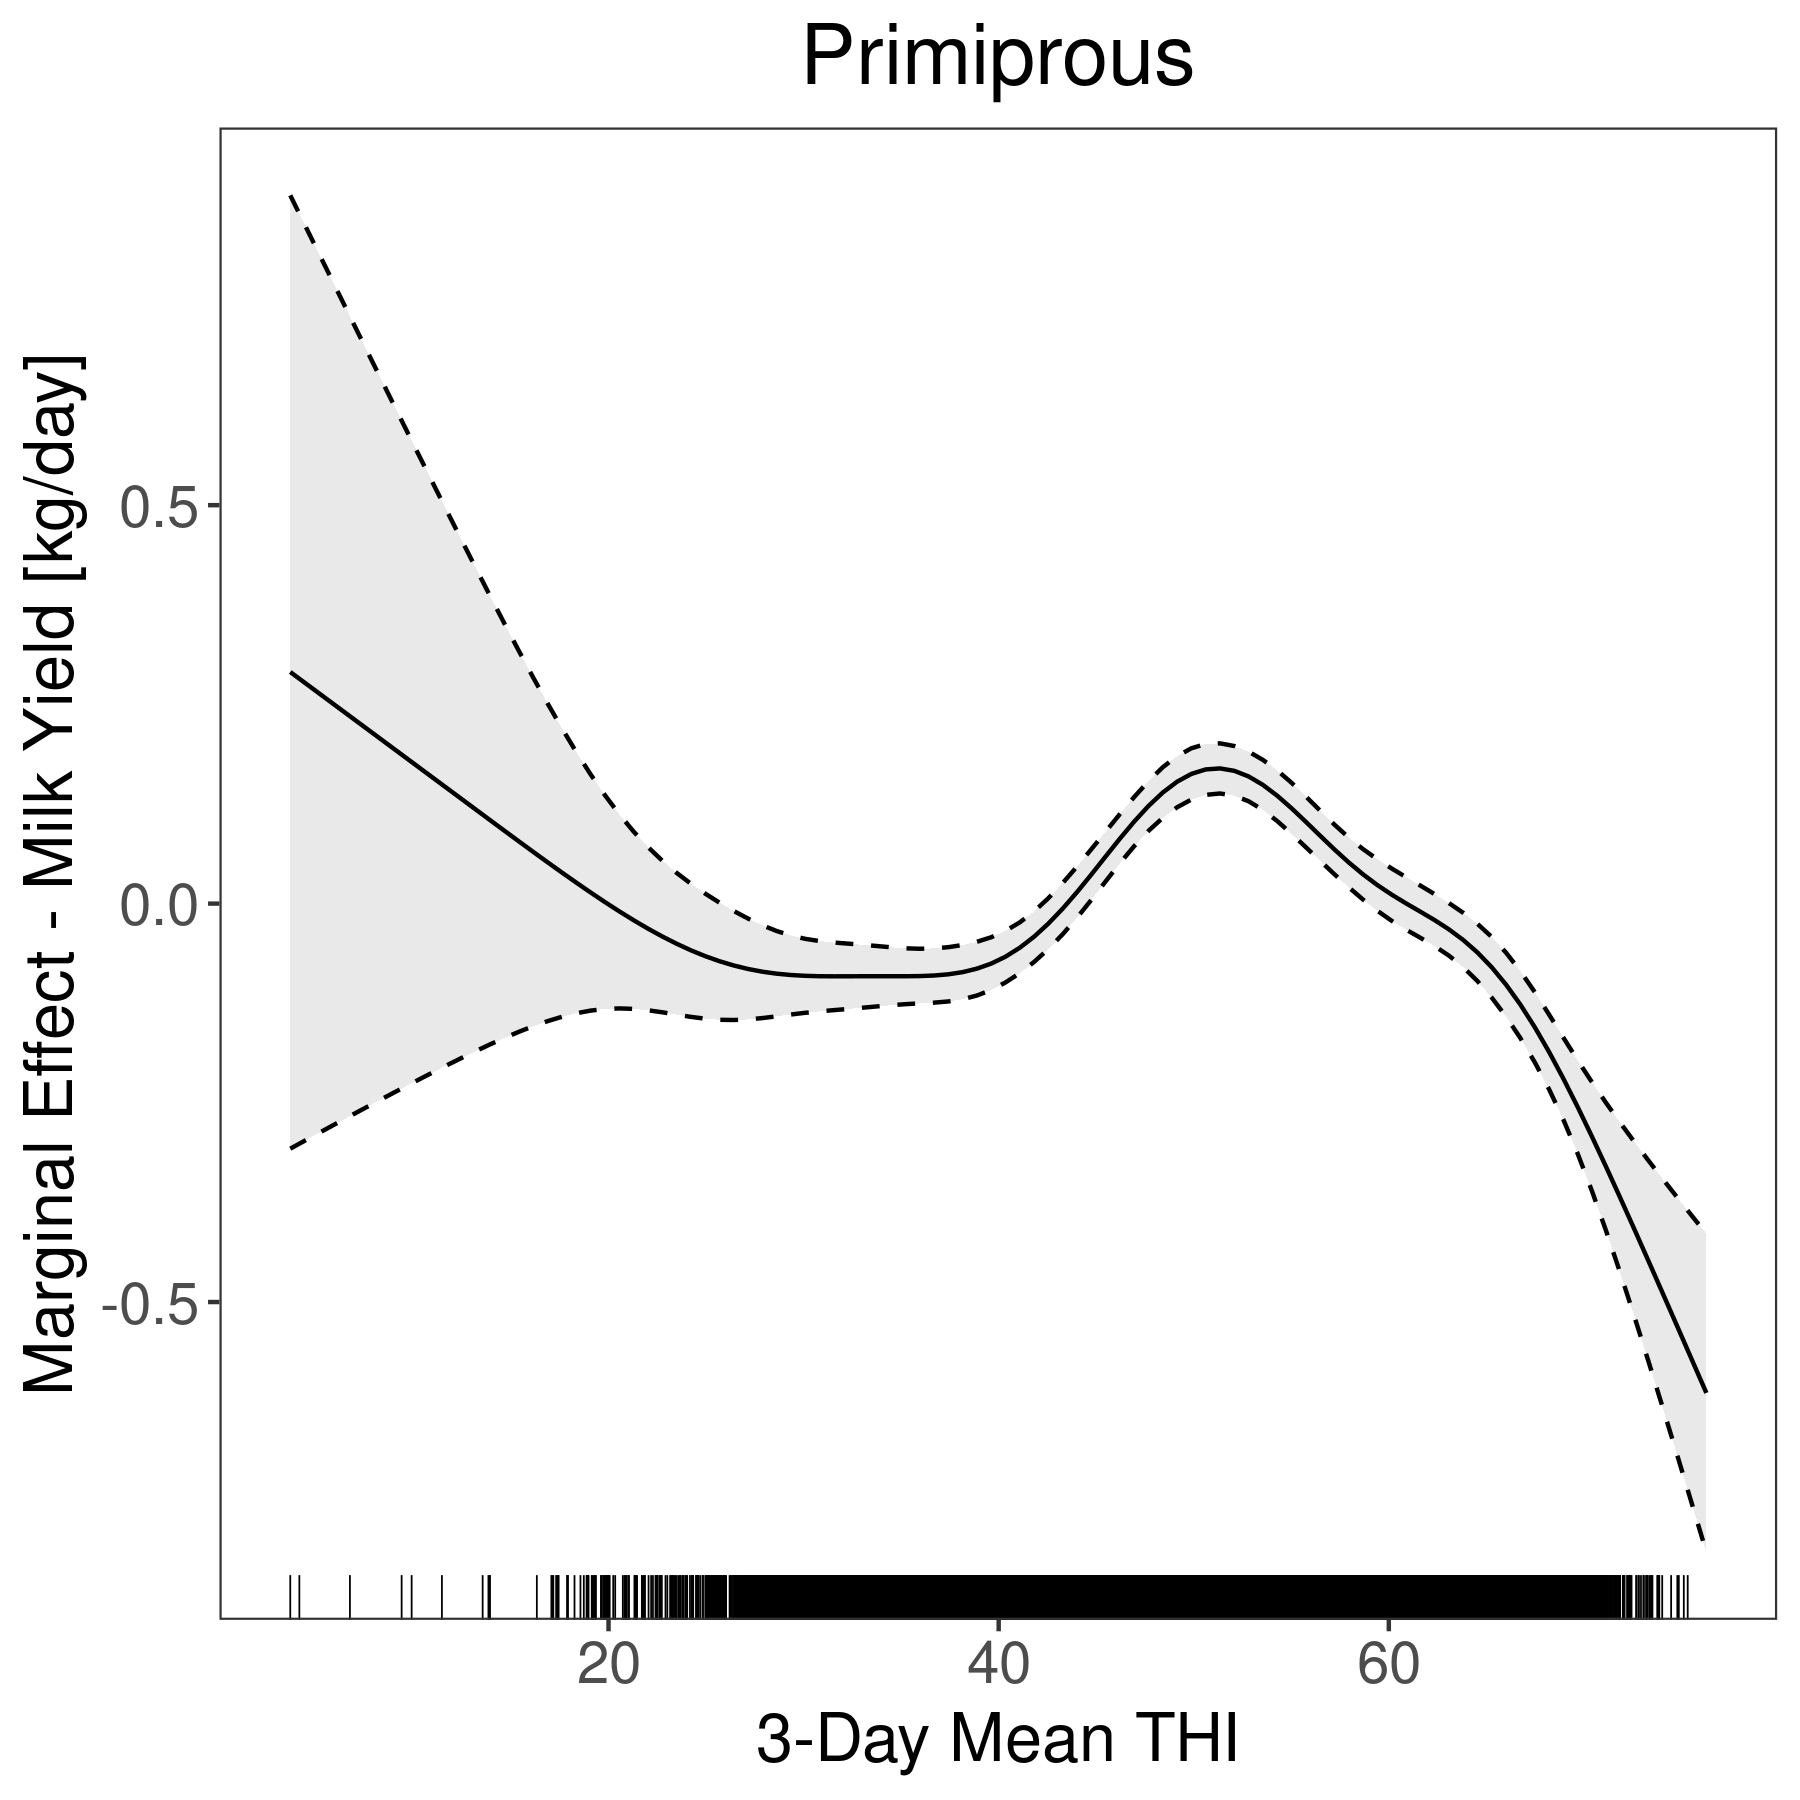
\includegraphics[width=\textwidth]{thesis/figures/models/milk/after2010/ho_milk_after2010/ho_milk_after2010_marginal_thi_milk_primi.png}
    \end{subfigure}
    \hspace{0.05\textwidth} % Optional space between the figures
    \begin{subfigure}[b]{0.45\textwidth}
        \centering
        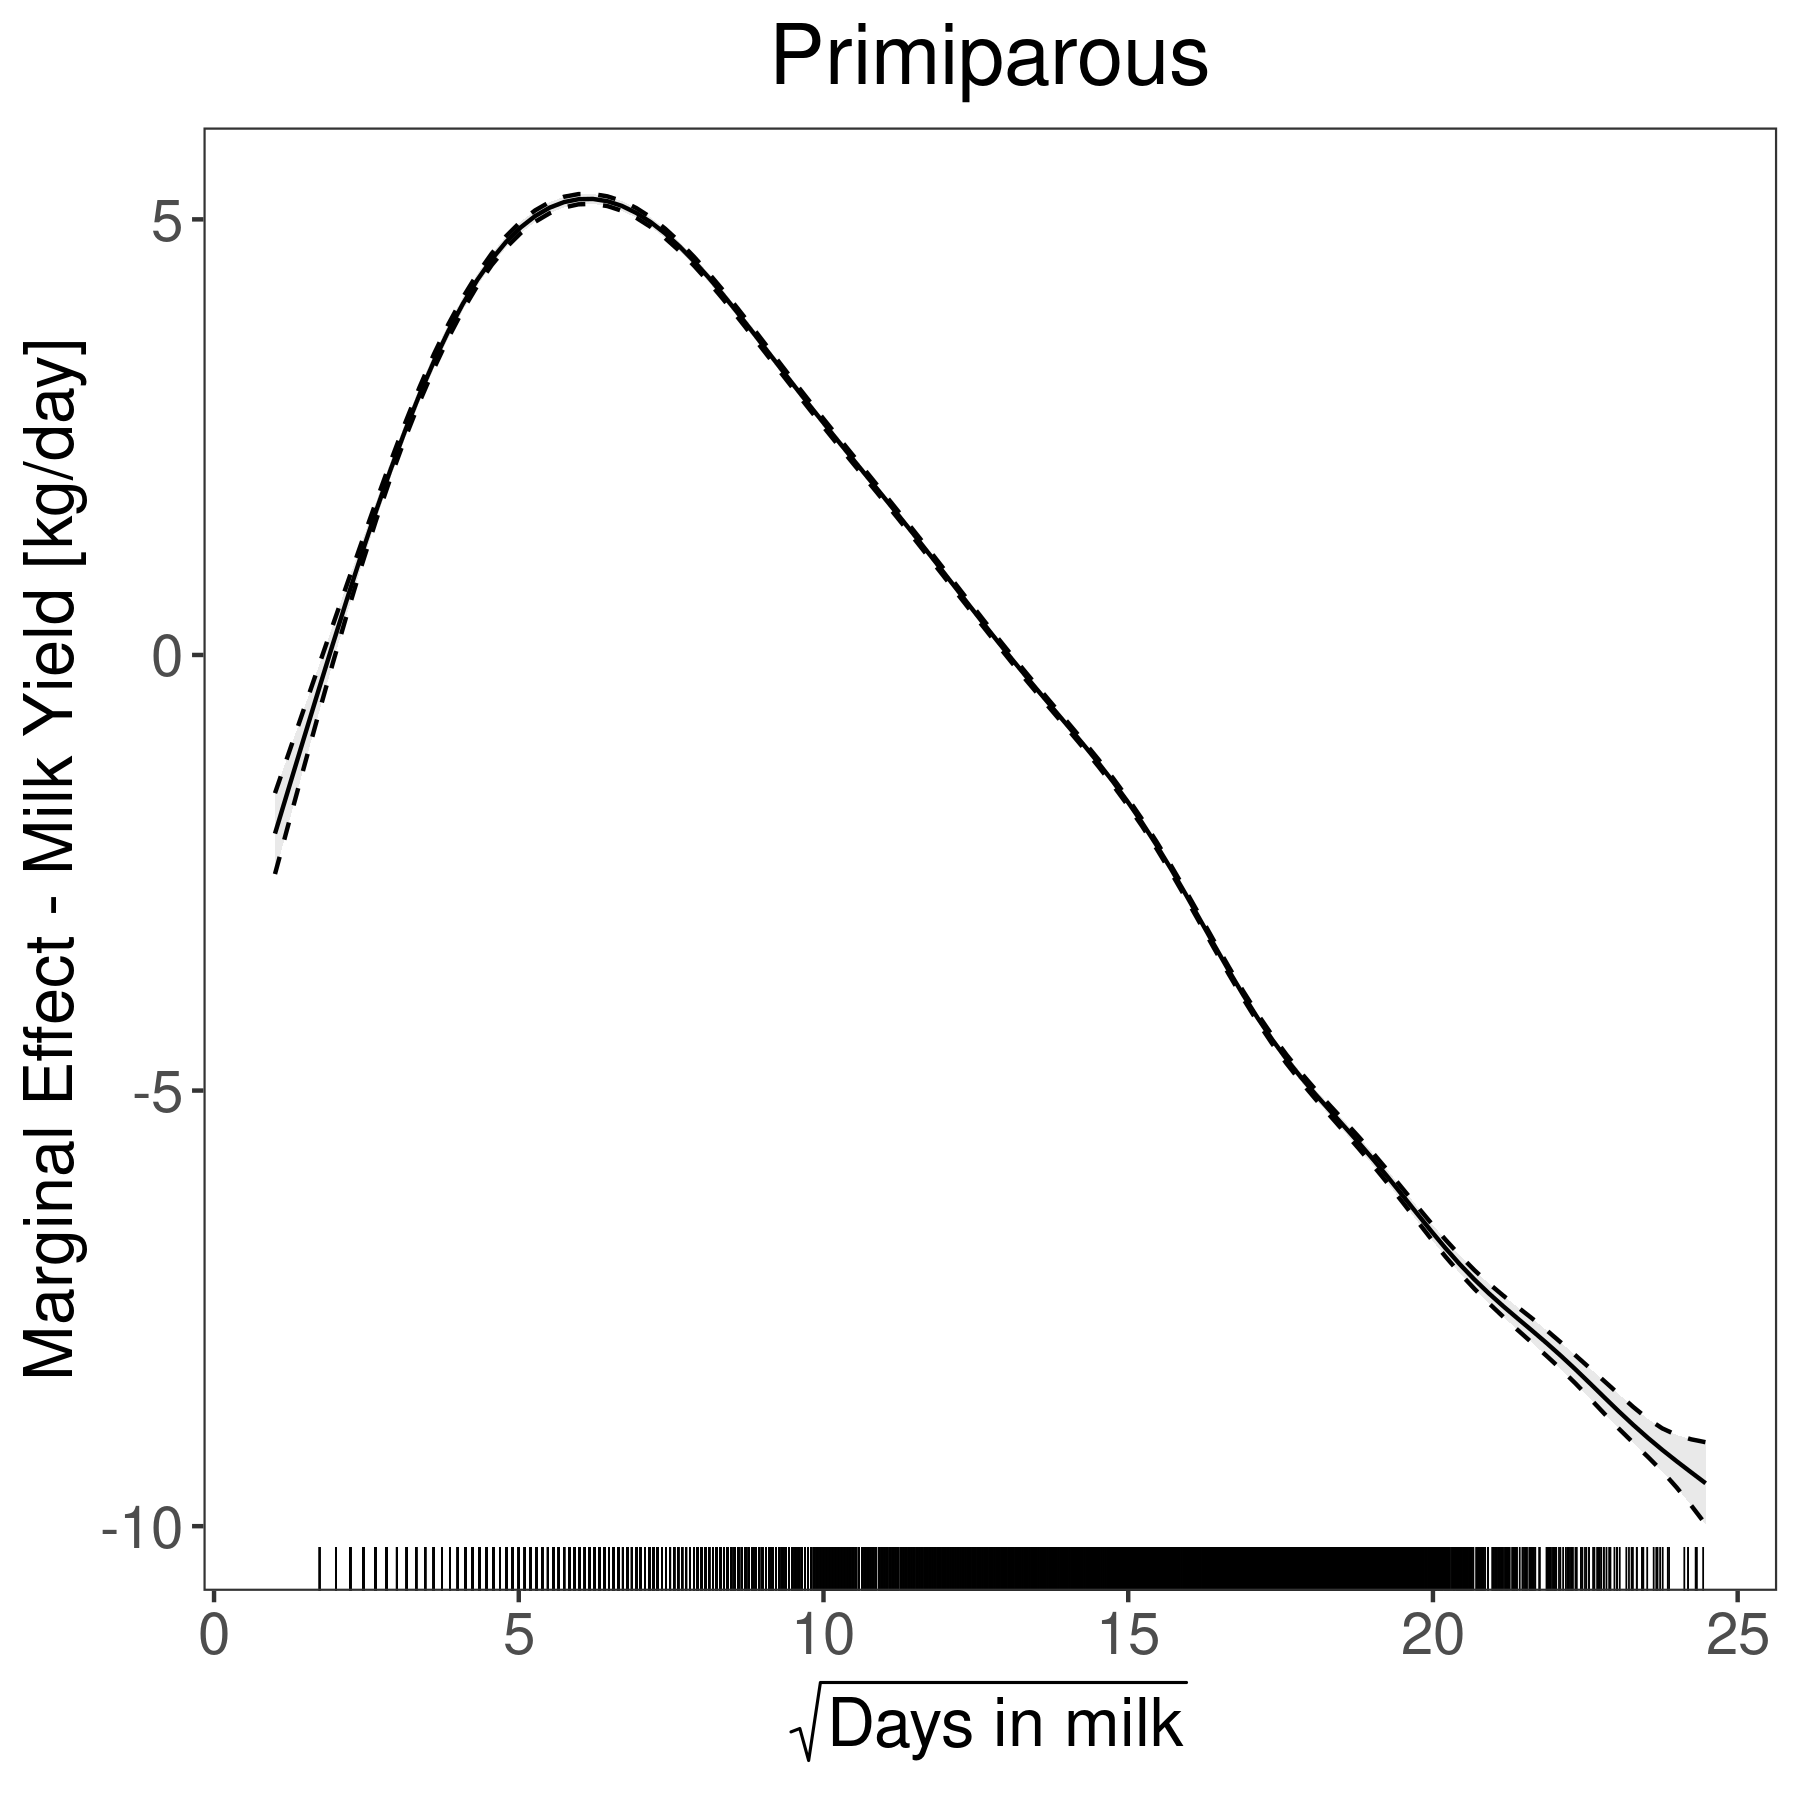
\includegraphics[width=\textwidth]{thesis/figures/models/milk/after2010/ho_milk_after2010/ho_milk_after2010_marginal_dim_milk_primi.png}
    \end{subfigure}
    \begin{subfigure}[b]{0.45\textwidth}
        \centering
        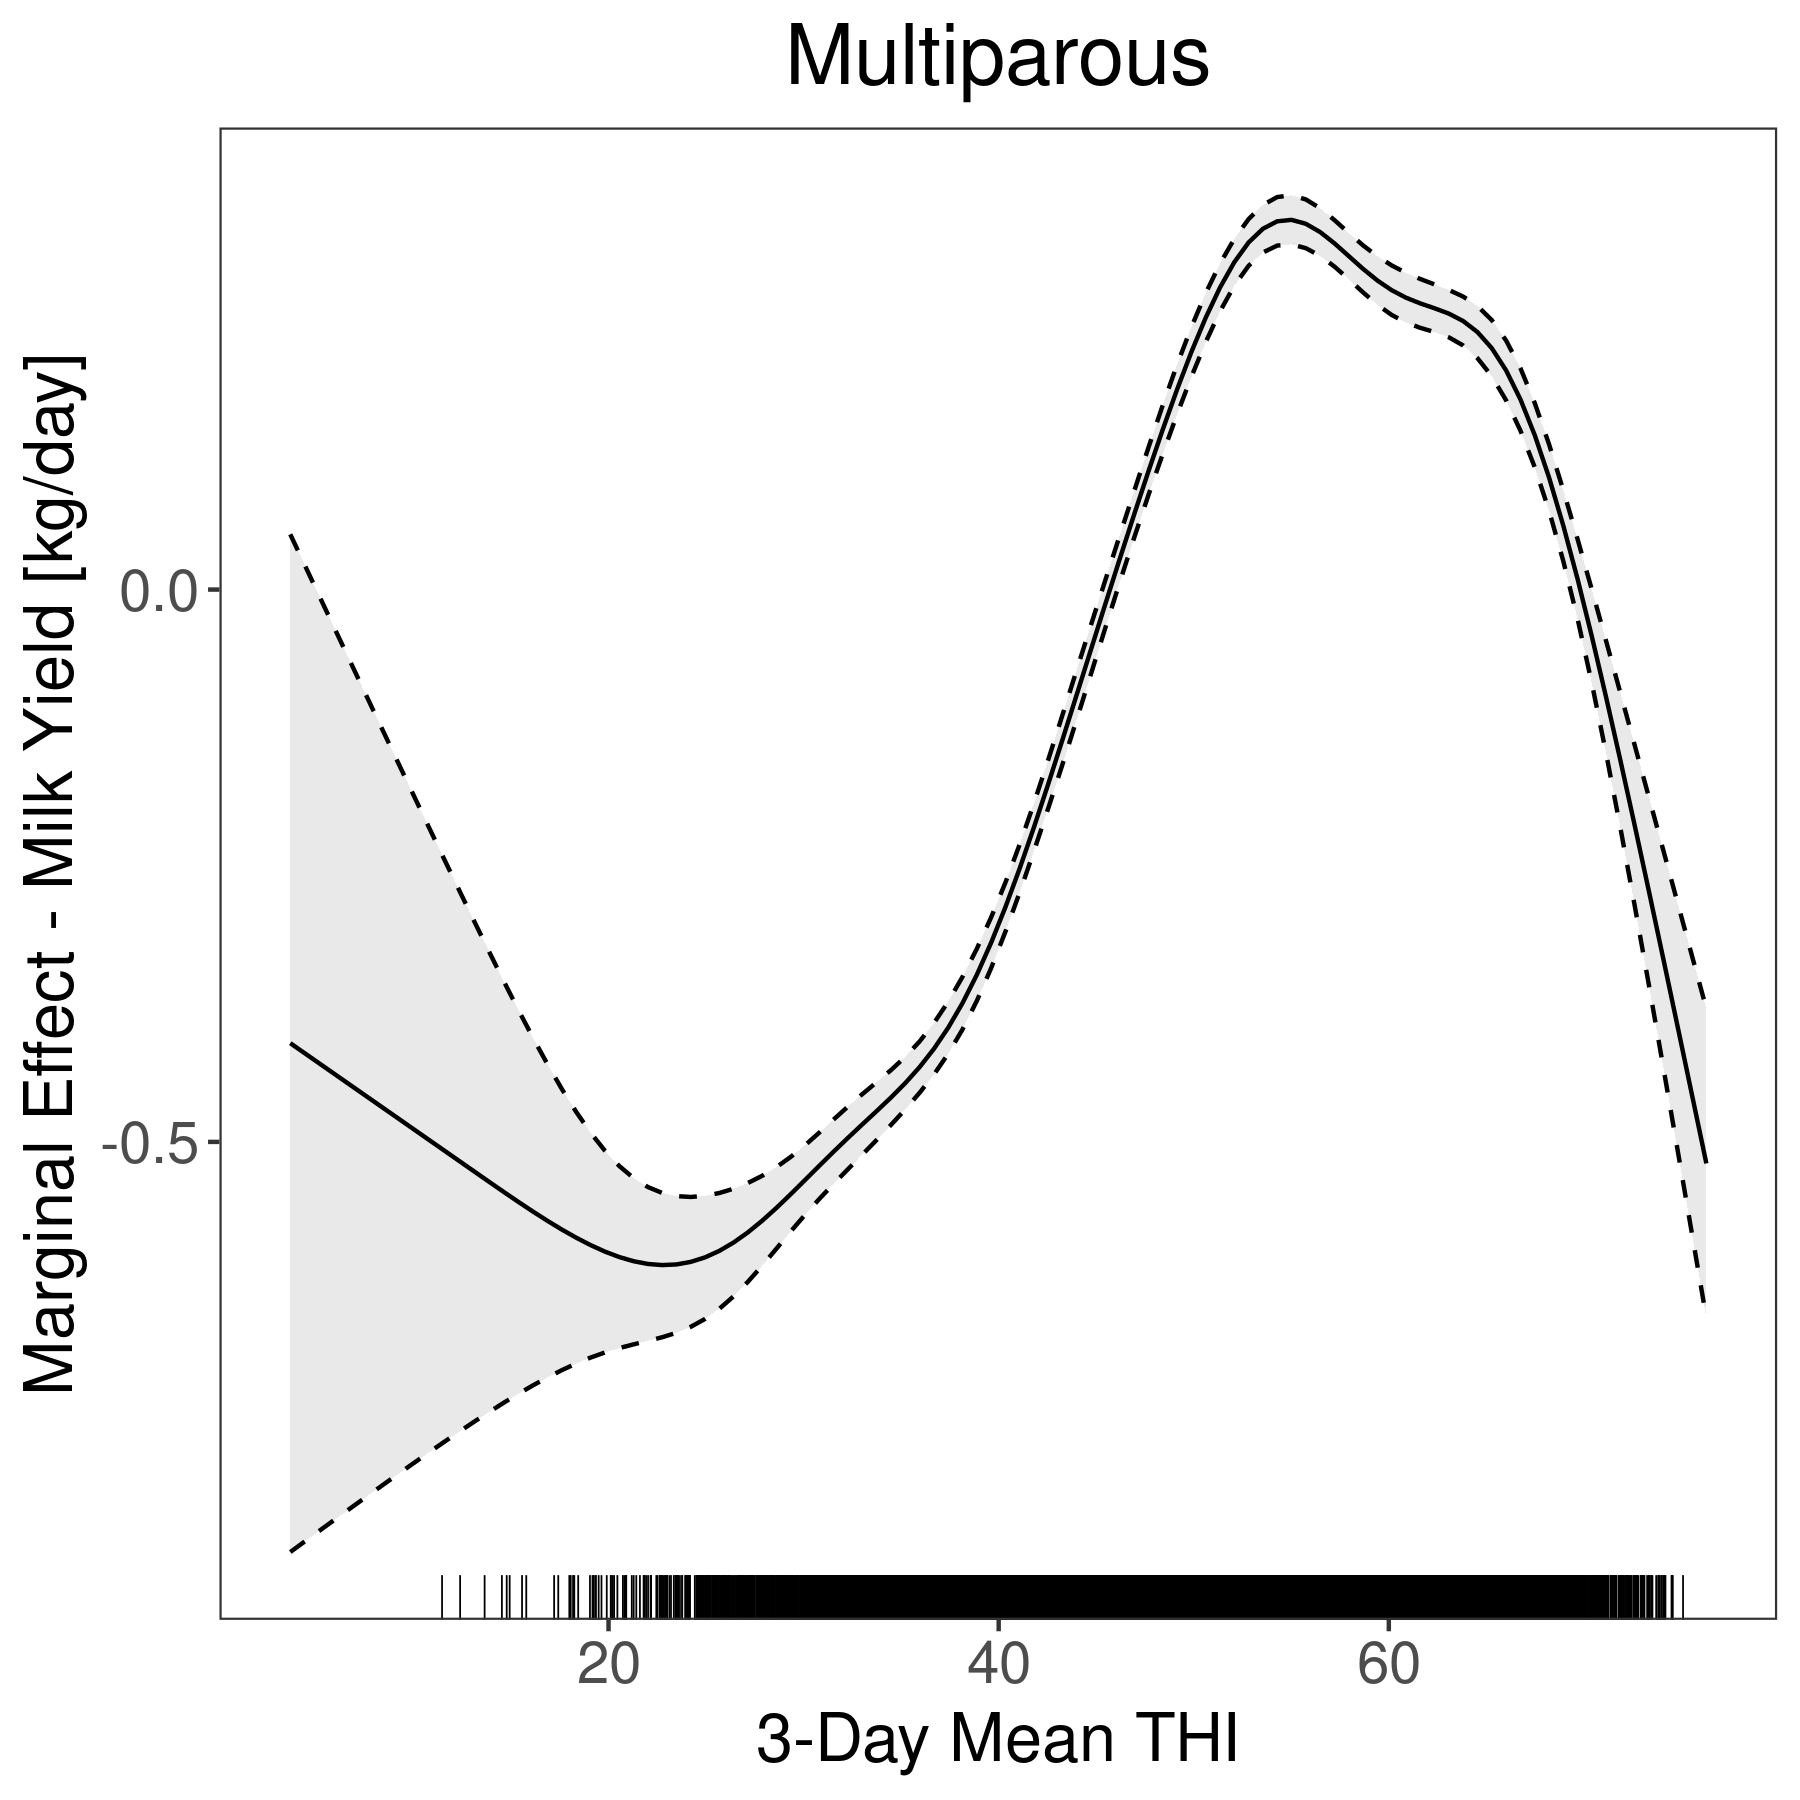
\includegraphics[width=\textwidth]{thesis/figures/models/milk/after2010/ho_milk_after2010/ho_milk_after2010_marginal_thi_milk_multi.png}
    \end{subfigure}
    \hspace{0.05\textwidth} % Optional space between the figures
    \begin{subfigure}[b]{0.45\textwidth}
        \centering
        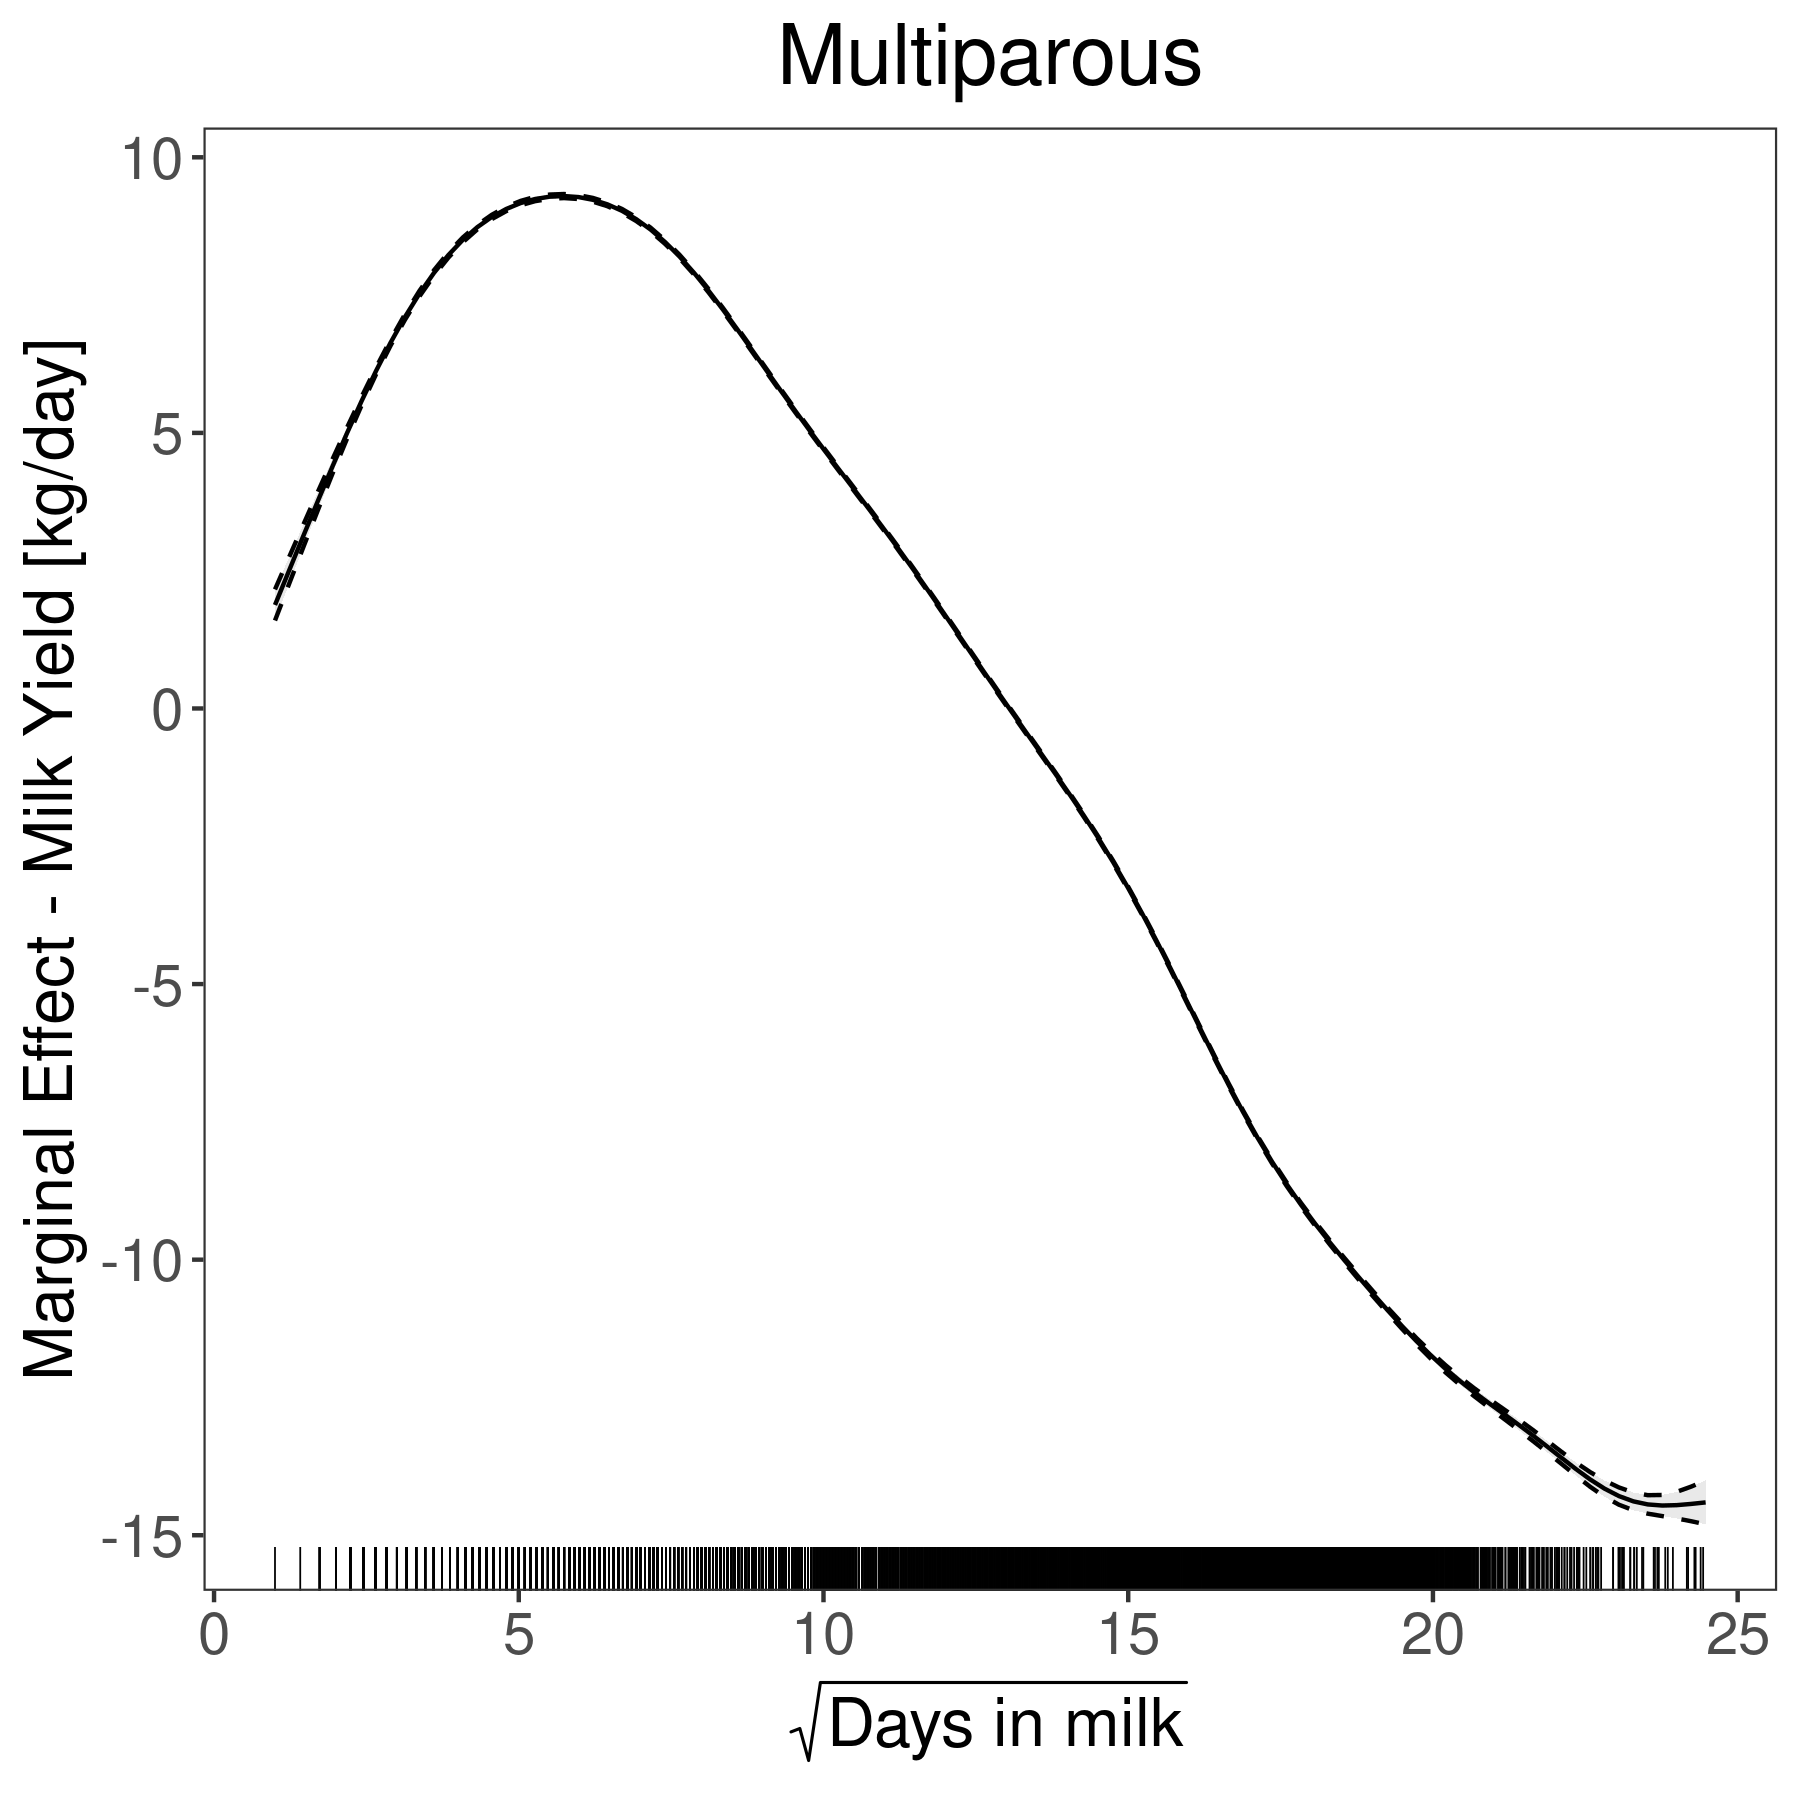
\includegraphics[width=\textwidth]{thesis/figures/models/milk/after2010/ho_milk_after2010/ho_milk_after2010_marginal_dim_milk_multi.png}
    \end{subfigure}
    \caption[]{Holstein: Milk Yield - 2010 - 2023 - THI Effect and Lactation Curve}
    \label{fig:main}
\end{figure}
\addtocontents{toc}{\protect\setcounter{tocdepth}{2}}

\section{Holstein: ECM Yield}
\subsection{Full Period: 1985-2023}\label{model:ho_ecm_full}
\paragraph{Model Summary} \quad \\

    \begin{table}[H]
    \centering
    \begin{tabular}{lrrrr}
    \textbf{A. parametric coefficients} & Estimate & Std. Error & t-value & p-value \\ 
       \hline
       \hline
  (Intercept) & 20.1076 & 0.1617 & 124.3358 & $<$ 0.0001 \\ 
  parityprimiparous & -3.9424 & 0.0093 & -422.7197 & $<$ 0.0001 \\ 
  year1986 & 0.1635 & 0.1304 & 1.2541 & 0.2098 \\ 
  year1987 & -0.1100 & 0.1299 & -0.8464 & 0.3973 \\ 
  year1988 & -0.4448 & 0.1288 & -3.4531 & 0.0006 \\ 
  year1989 & 0.1254 & 0.1278 & 0.9809 & 0.3267 \\ 
  year1990 & 0.5707 & 0.1281 & 4.4557 & $<$ 0.0001 \\ 
  year1991 & 0.7665 & 0.1268 & 6.0465 & $<$ 0.0001 \\ 
  year1992 & 1.1648 & 0.1260 & 9.2442 & $<$ 0.0001 \\ 
  year1993 & 1.2702 & 0.1250 & 10.1623 & $<$ 0.0001 \\ 
  year1994 & 0.9399 & 0.1233 & 7.6238 & $<$ 0.0001 \\ 
  year1995 & 1.3246 & 0.1236 & 10.7206 & $<$ 0.0001 \\ 
  year1996 & 1.7648 & 0.1222 & 14.4466 & $<$ 0.0001 \\ 
  year1997 & 2.3101 & 0.1223 & 18.8938 & $<$ 0.0001 \\ 
  year1998 & 2.9914 & 0.1206 & 24.8069 & $<$ 0.0001 \\ 
  year1999 & 2.6437 & 0.1193 & 22.1562 & $<$ 0.0001 \\ 
  year2000 & 2.5987 & 0.1186 & 21.9127 & $<$ 0.0001 \\ 
  year2001 & 2.9072 & 0.1179 & 24.6612 & $<$ 0.0001 \\ 
  year2002 & 3.0868 & 0.1175 & 26.2770 & $<$ 0.0001 \\ 
  year2003 & 3.5531 & 0.1171 & 30.3539 & $<$ 0.0001 \\ 
  year2004 & 4.0984 & 0.1169 & 35.0471 & $<$ 0.0001 \\ 
  year2005 & 4.7114 & 0.1167 & 40.3673 & $<$ 0.0001 \\ 
  year2006 & 4.6636 & 0.1166 & 39.9990 & $<$ 0.0001 \\ 
  year2007 & 4.3704 & 0.1165 & 37.5094 & $<$ 0.0001 \\ 
  year2008 & 4.7638 & 0.1164 & 40.9126 & $<$ 0.0001 \\ 
  year2009 & 5.1818 & 0.1165 & 44.4952 & $<$ 0.0001 \\ 
  year2010 & 5.8336 & 0.1164 & 50.1183 & $<$ 0.0001 \\ 
  year2011 & 6.0286 & 0.1164 & 51.7791 & $<$ 0.0001 \\ 
  year2012 & 6.1847 & 0.1167 & 53.0014 & $<$ 0.0001 \\ 
  year2013 & 5.7015 & 0.1168 & 48.8341 & $<$ 0.0001 \\ 
  year2014 & 6.3304 & 0.1167 & 54.2257 & $<$ 0.0001 \\ 
  year2015 & 6.7851 & 0.1168 & 58.0841 & $<$ 0.0001 \\ 
  year2016 & 7.3041 & 0.1170 & 62.4072 & $<$ 0.0001 \\ 
  year2017 & 7.3981 & 0.1169 & 63.2676 & $<$ 0.0001 \\ 
  year2018 & 8.0557 & 0.1171 & 68.8206 & $<$ 0.0001 \\ 
  year2019 & 8.2896 & 0.1171 & 70.8058 & $<$ 0.0001 \\ 
  year2020 & 8.9829 & 0.1174 & 76.5305 & $<$ 0.0001 \\ 
  year2021 & 9.5582 & 0.1170 & 81.6686 & $<$ 0.0001 \\ 
  year2022 & 9.6665 & 0.1169 & 82.6636 & $<$ 0.0001 \\ 
  year2023 & 10.4348 & 0.1167 & 89.4257 & $<$ 0.0001 \\ 
       \hline
    \textbf{B. smooth terms} & edf & Ref.df & F-value & p-value \\ 
    \hline
    \hline
  s(thi\_mean\_t0\_3d):paritymultiparous & 8.2862 & 8.2862 & 226.9355 & $<$ 0.0001 \\ 
  s(thi\_mean\_t0\_3d):parityprimiparous & 6.8141 & 6.8141 & 229.3868 & $<$ 0.0001 \\ 
  s(days\_in\_milk\_t):paritymultiparous & 13.5893 & 13.5893 & 104352.5853 & $<$ 0.0001 \\ 
  s(days\_in\_milk\_t):parityprimiparous & 12.9465 & 12.9465 & 10972.7975 & $<$ 0.0001 \\
       \hline
    \end{tabular}
    \caption[]{Holstein: ECM Yield - 1985-2023 - GAMM model summary without random effect terms.}
    \end{table}

\newpage
\begin{table}[H]
\centering
\begin{tabular}
{l | r | r | r | r}
\textbf{Smooth Term Fixed Effect} & Est. & SE & z & p\\
\hline
\hline
s(thi\_mean\_t0\_3d):multiFx1 & 0.638531  &  0.115151   & 5.55 &  $<$ 1e-07 \\
s(thi\_mean\_t0\_3d):primiFx1 & 0.559616  &  0.129725   &  4.31  &  $<$ 1e-04\\
s(days\_in\_milk\_):multiFx1 &  1.239    & 0.456686 &   2.71  &  0.0067\\
s(days\_in\_milk\_):primiFx1 & 2.33168  &   0.535407  &   4.35  &  $<$ 1e-04\\
\hline
\textbf{Variance Component} & Estimated $\sigma$ & & & \\
\hline
\hline
$\sigma_\alpha$ & 3.11752 & &  & \\
$\sigma_\iota$ & 1.07133 & & & \\
$\sigma_\phi$ & 3.47683 & & & \\
s(thi\_mean\_t0\_3d):multi & 2.15566 & & & \\
s(days\_in\_milk\_):primi & 6.54541 & & & \\
s(days\_in\_milk\_):multi & 8.73852 & & & \\
s(thi\_mean\_t0\_3d):primi & 1.38212 & & & \\
Residual & 4.16782 & & & \\
\end{tabular}
\caption[]{Holstein: ECM Yield - 1985-2023 - Mixed Model Summary - Smooth Terms and Random Effects.}
\end{table}



\paragraph{Model Diagnostics} \quad \\
\begin{figure}[H]
    \centering
    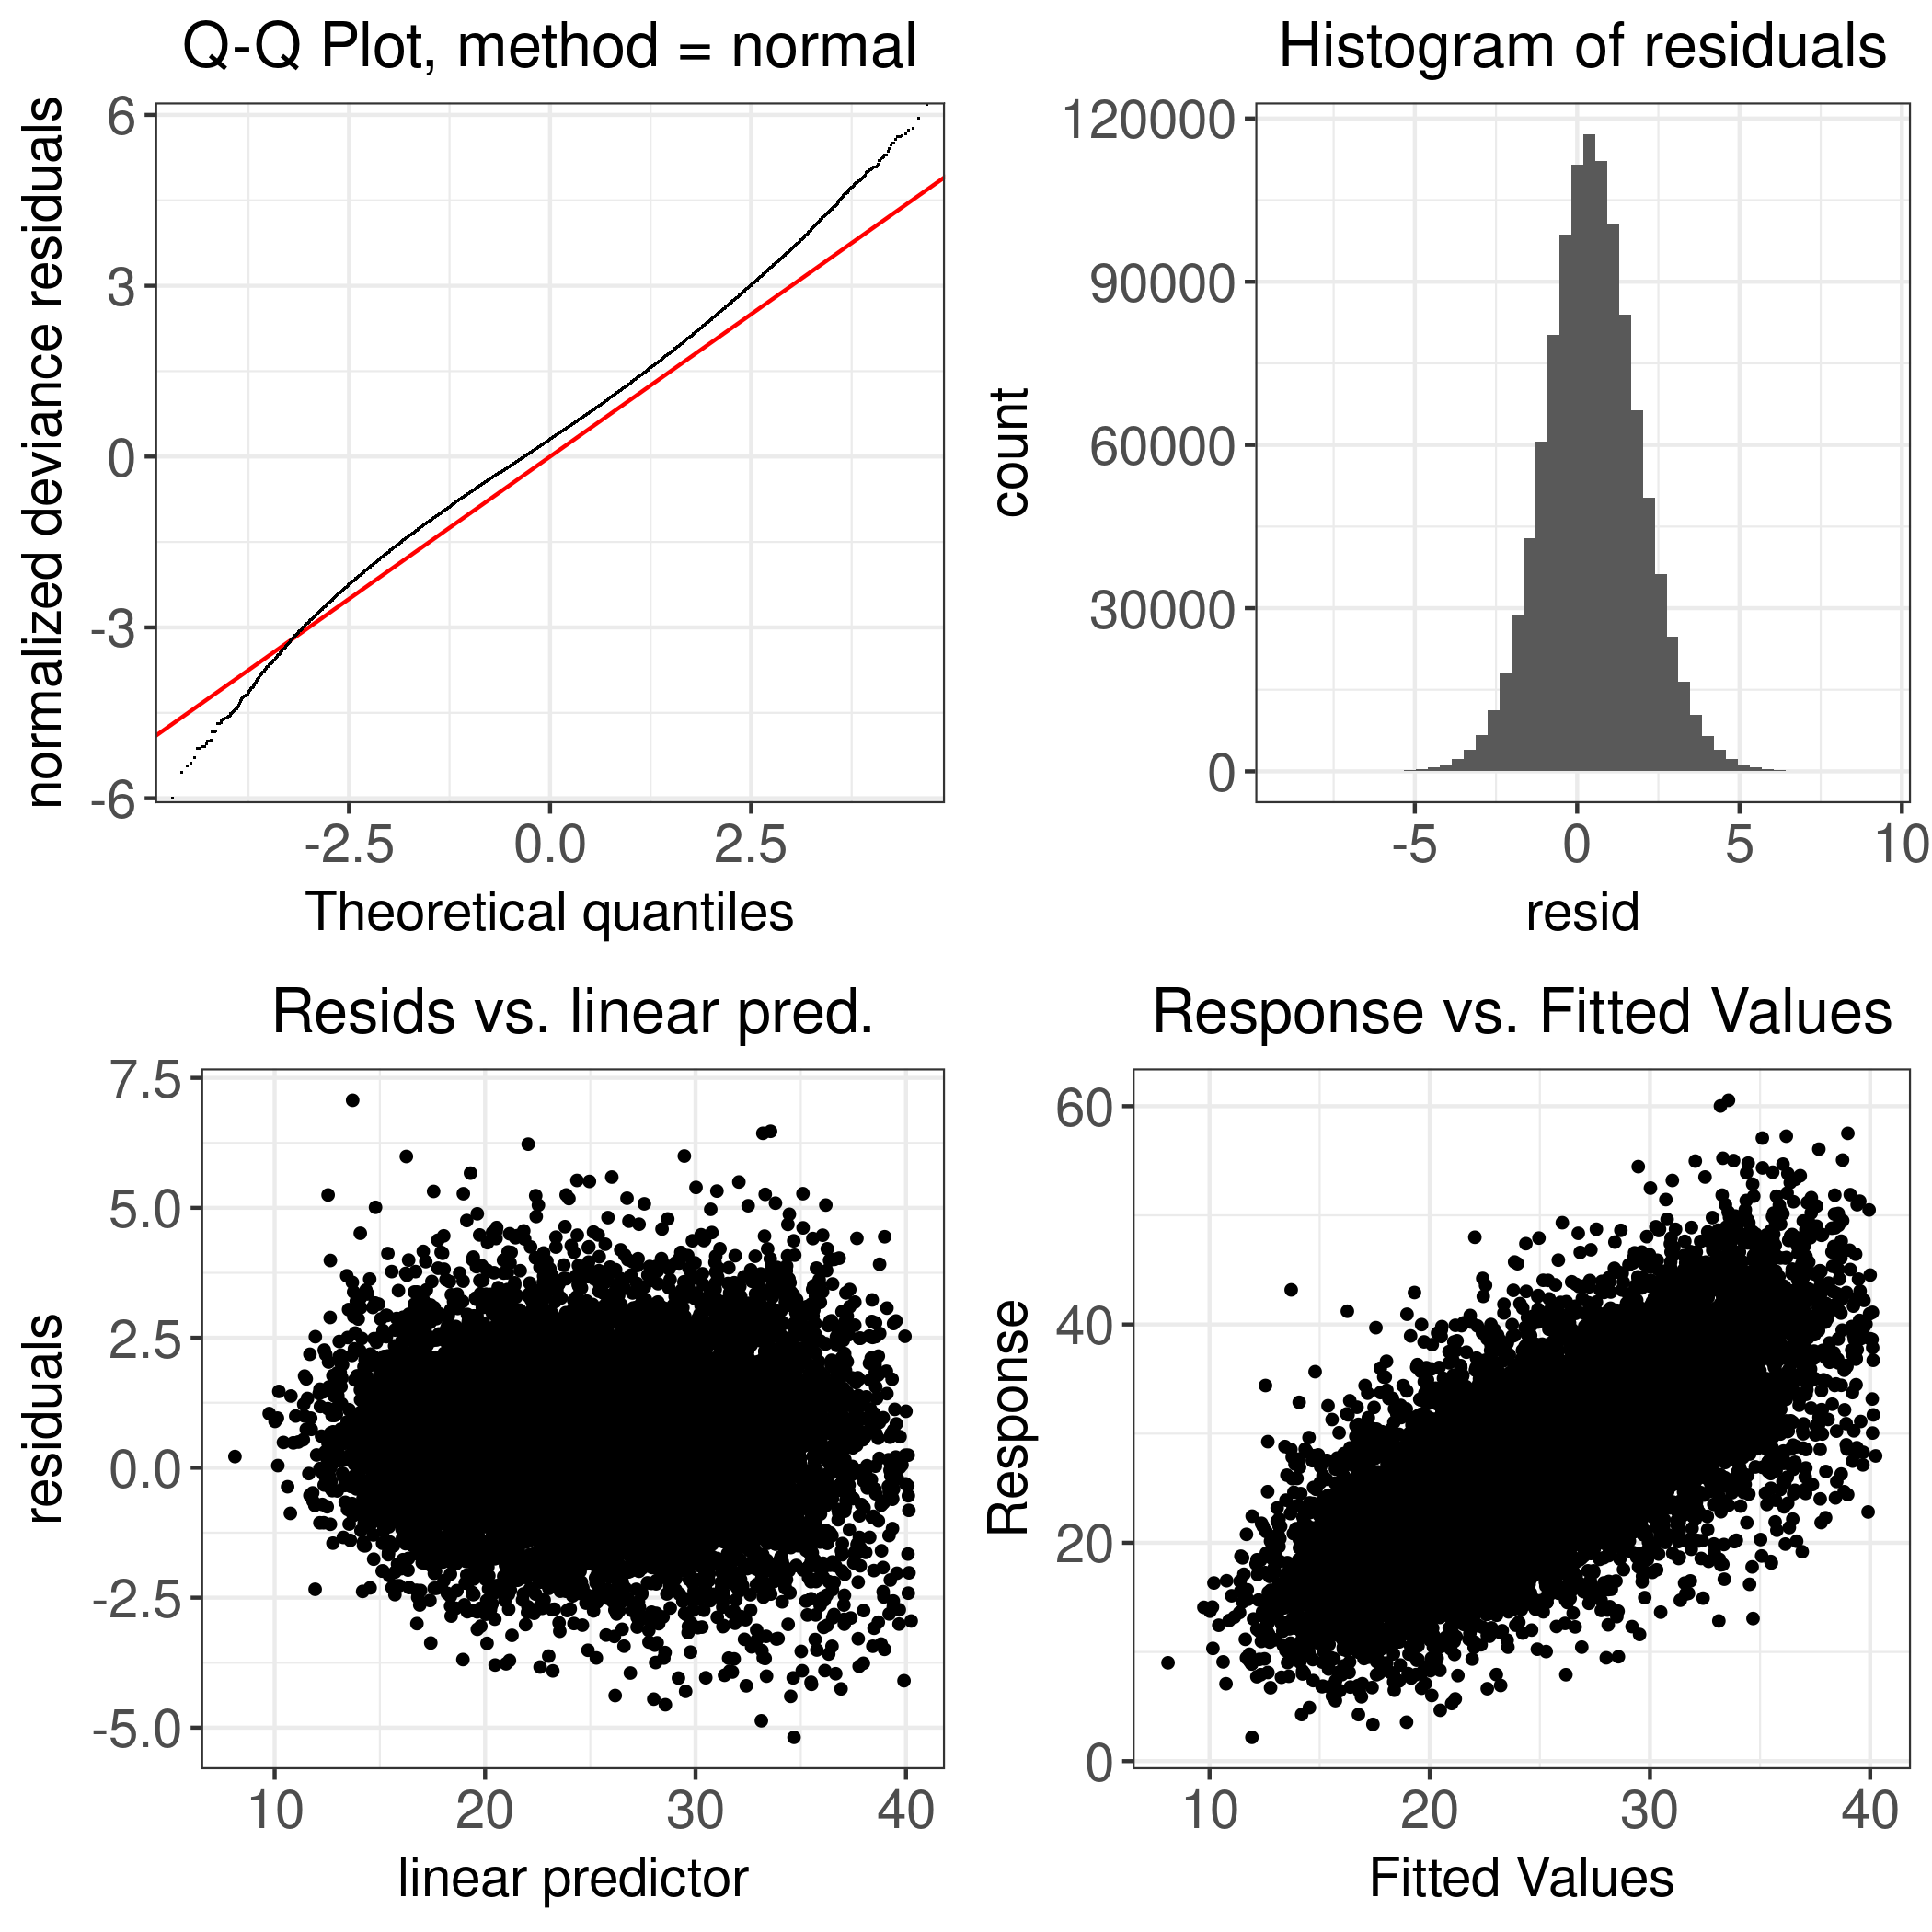
\includegraphics[width=0.6\textwidth]{thesis/figures/models/ecm/full/ho_ecm_full/ho_ecm_full_diagnostics.png}
    \caption[]{Holstein: ECM Yield - 1985-2023 - Diagnostic Plot}
\end{figure}

\newpage
\paragraph{THI Effect and Lactation Curve} \quad \\
\begin{figure}[H]
    \centering
    \begin{subfigure}[b]{0.45\textwidth}
        \centering
        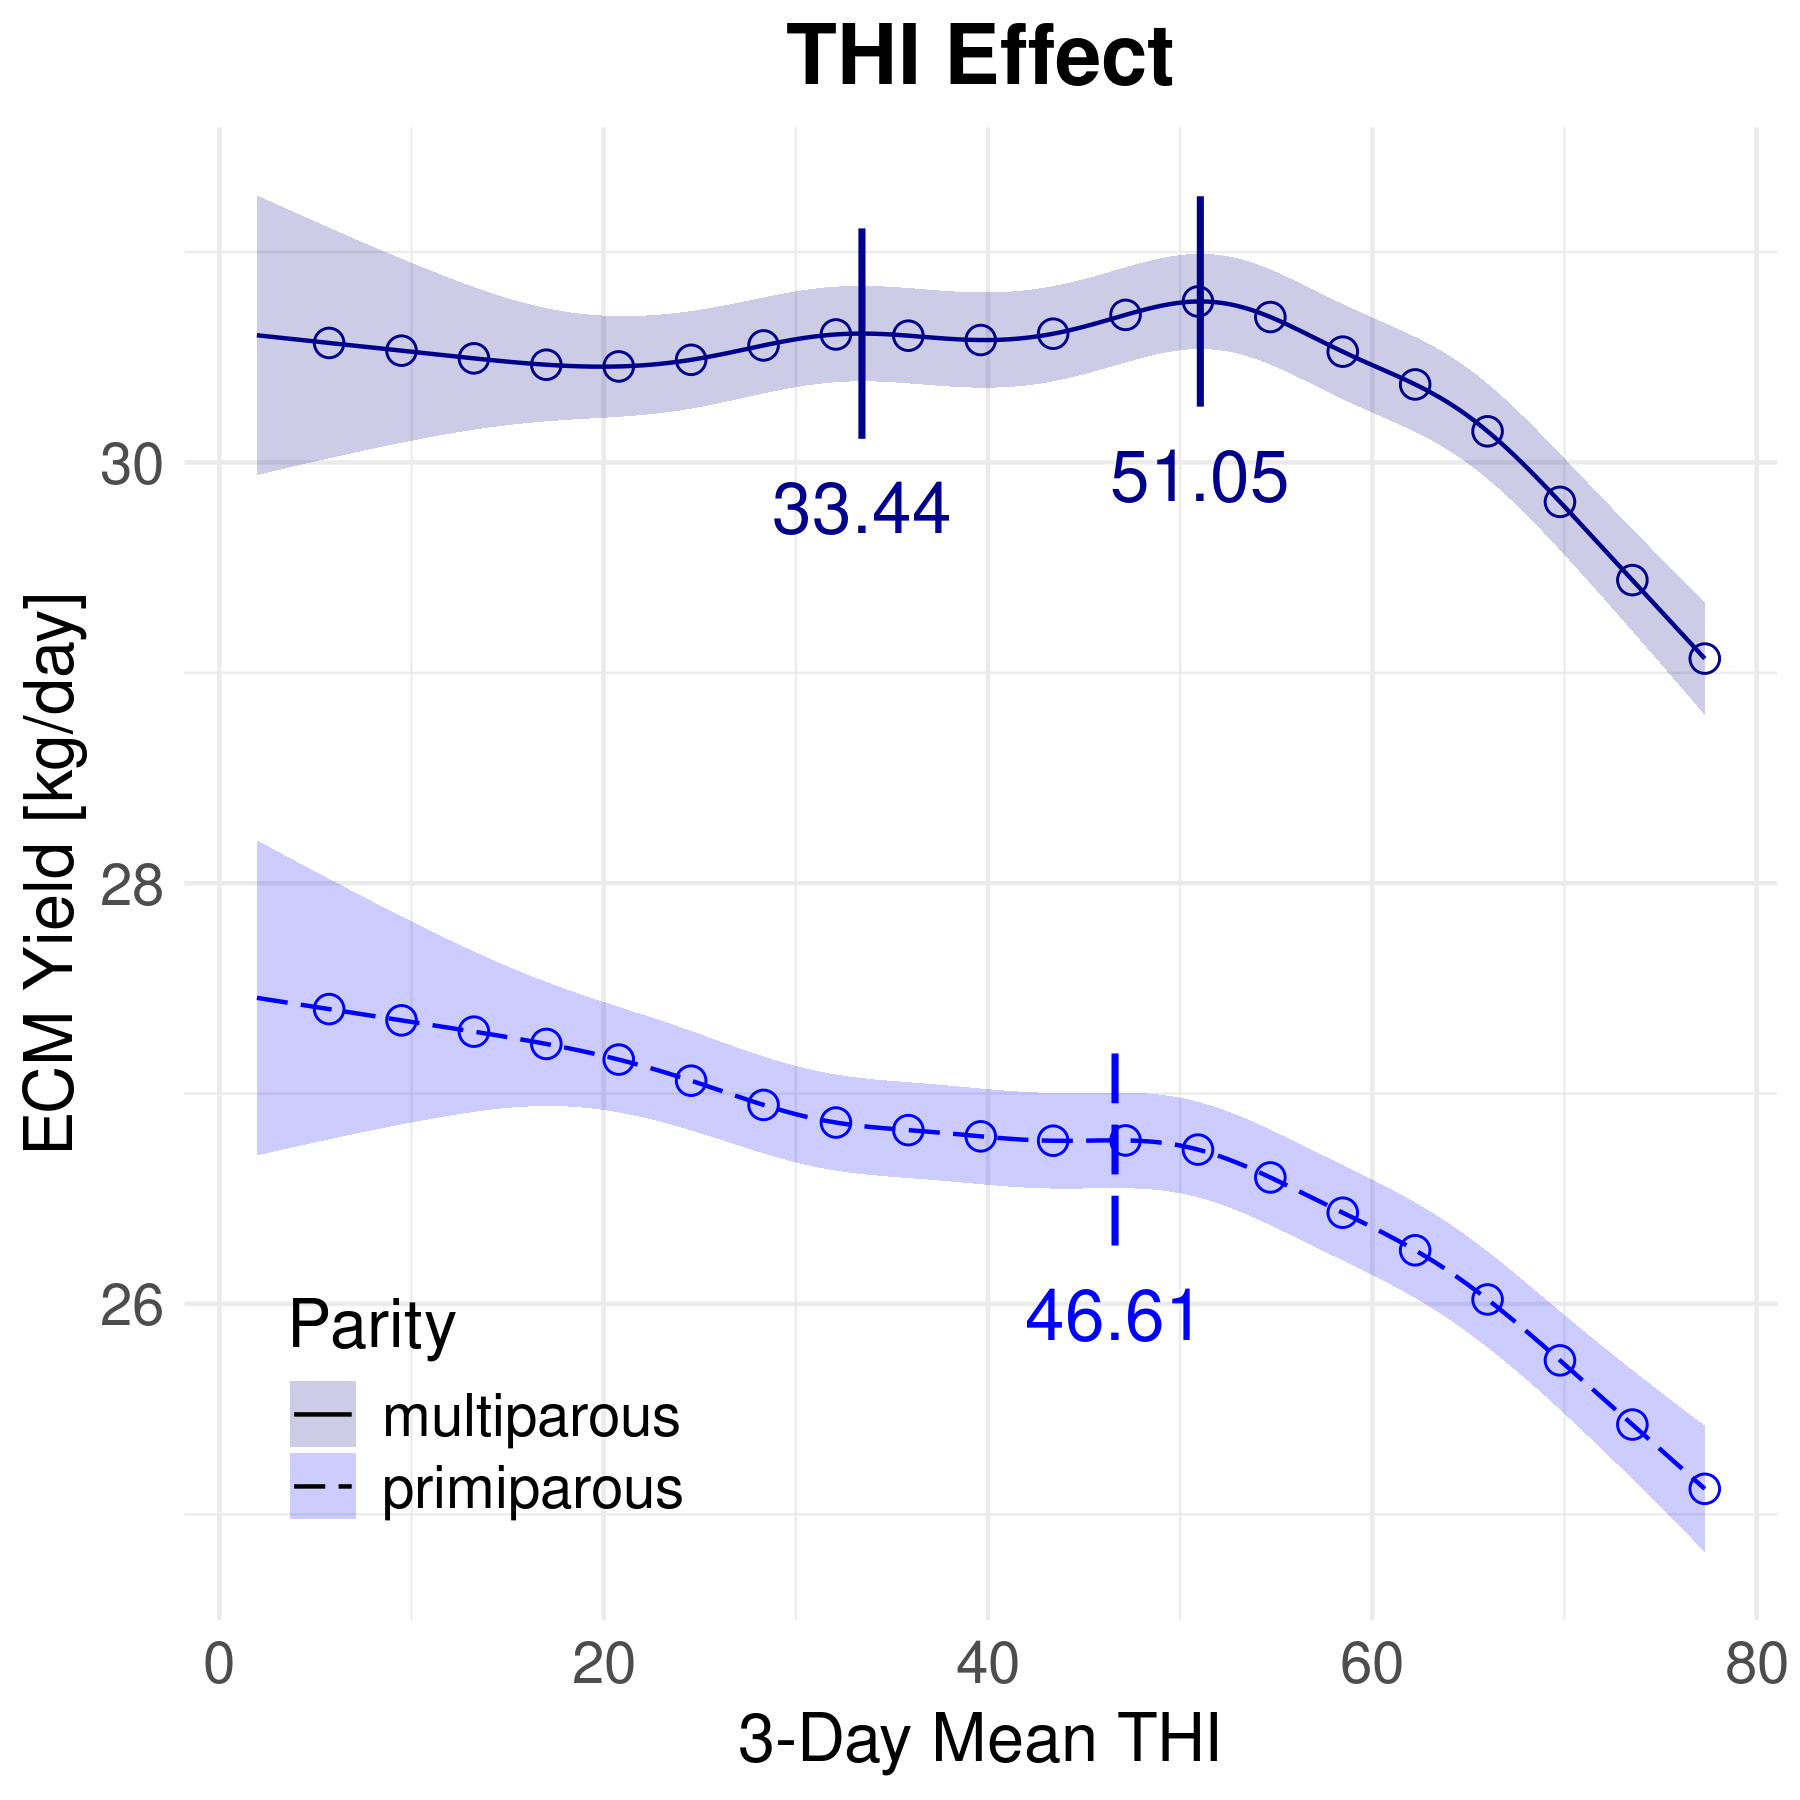
\includegraphics[width=\textwidth]{thesis/figures/models/ecm/full/ho_ecm_full/ho_ecm_full_marginal_thi_milk_combined.png}
    \end{subfigure}
    \hspace{0.05\textwidth} % Optional space between the figures
    \begin{subfigure}[b]{0.45\textwidth}
        \centering
        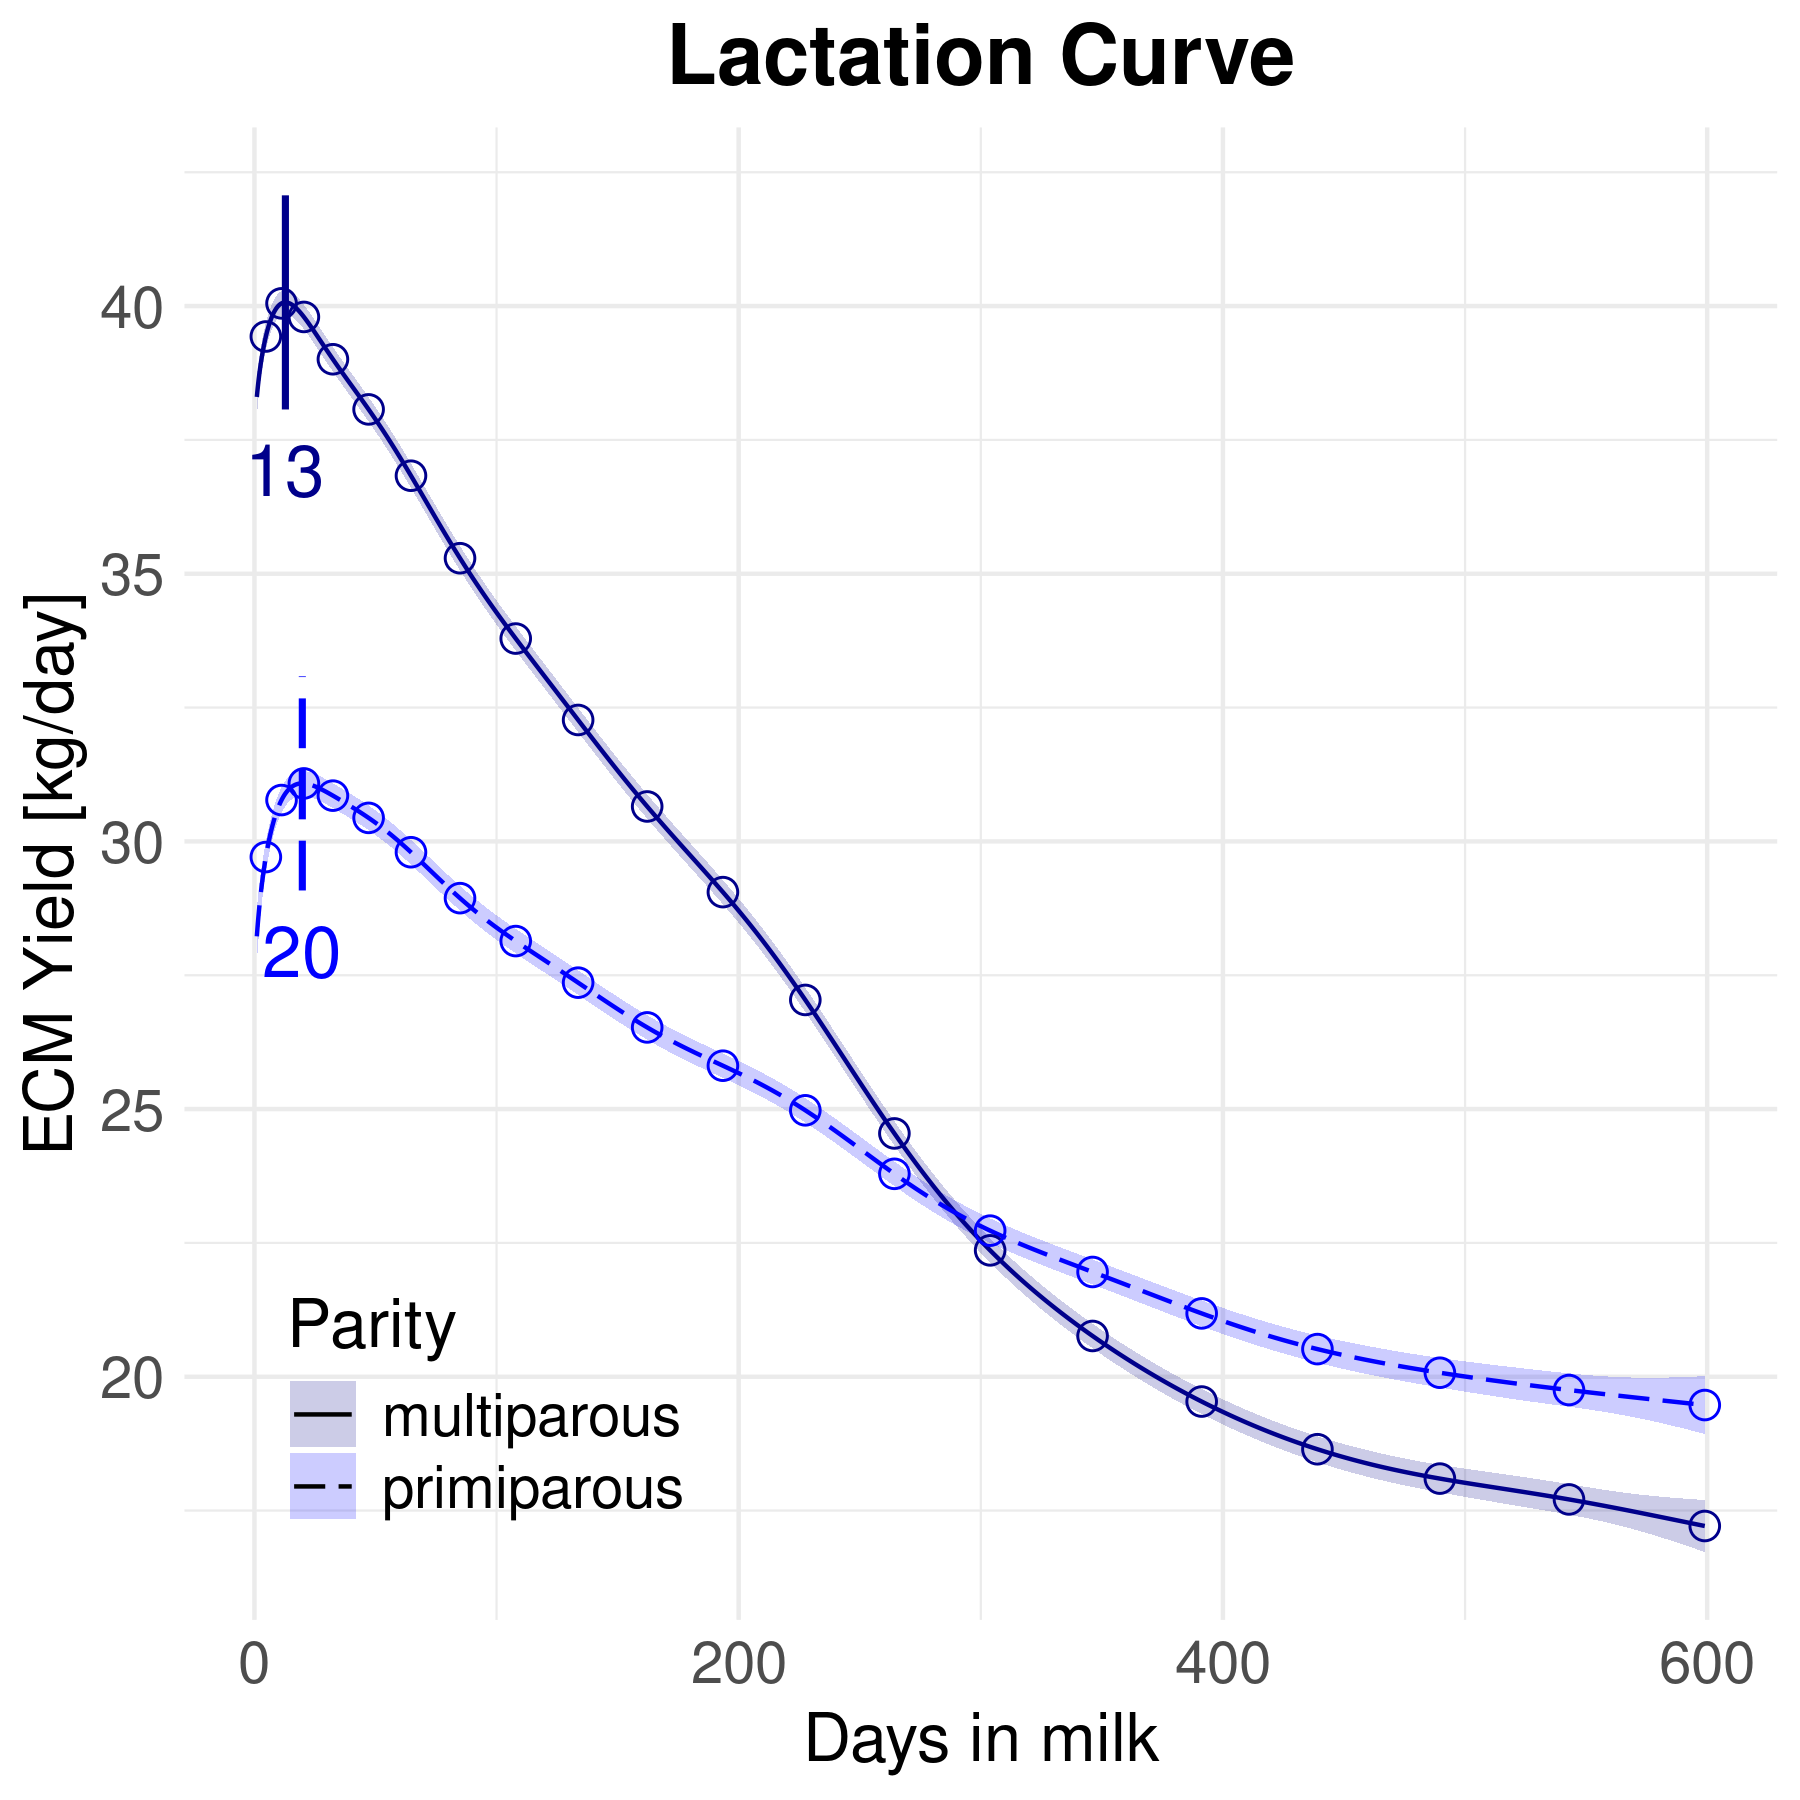
\includegraphics[width=\textwidth]{thesis/figures/models/ecm/full/ho_ecm_full/ho_ecm_full_marginal_dim_milk_combined.png}
    \end{subfigure}
    \begin{subfigure}[b]{0.45\textwidth}
        \centering
        \includegraphics[width=\textwidth]{thesis/figures/models/ecm/full/ho_ecm_full/ho_ecm_full_marginal_thi_milk_primi.png}
    \end{subfigure}
    \hspace{0.05\textwidth} % Optional space between the figures
    \begin{subfigure}[b]{0.45\textwidth}
        \centering
        \includegraphics[width=\textwidth]{thesis/figures/models/ecm/full/ho_ecm_full/ho_ecm_full_marginal_dim_milk_primi.png}
    \end{subfigure}
    \begin{subfigure}[b]{0.45\textwidth}
        \centering
        \includegraphics[width=\textwidth]{thesis/figures/models/ecm/full/ho_ecm_full/ho_ecm_full_marginal_thi_milk_multi.png}
    \end{subfigure}
    \hspace{0.05\textwidth} % Optional space between the figures
    \begin{subfigure}[b]{0.45\textwidth}
        \centering
        \includegraphics[width=\textwidth]{thesis/figures/models/ecm/full/ho_ecm_full/ho_ecm_full_marginal_dim_milk_multi.png}
    \end{subfigure}
    \caption[]{Holstein: ECM Yield - 1985 - 2023 - THI Effect and Lactation Curve}
    \label{fig:main}
\end{figure}


\subsection{Split Period: Until 2010 - After 2010}
\addtocontents{toc}{\protect\setcounter{tocdepth}{-1}}
\subsubsection{Split Period: 1985 - 2010}\label{model:ho_ecm_before}

\paragraph{Model Summary} \quad \\

    \begin{table}[H]
    \centering
    \begin{tabular}{lrrrr}
    \textbf{A. parametric coefficients} & Estimate & Std. Error & t-value & p-value \\ 
       \hline
       \hline
  (Intercept) & 19.5611 & 0.4528 & 43.2033 & $<$ 0.0001 \\ 
  parityprimiparous & -3.4047 & 0.0125 & -272.5784 & $<$ 0.0001 \\ 
  year1986 & 0.1564 & 0.2983 & 0.5244 & 0.6000 \\ 
  year1987 & -0.1604 & 0.3786 & -0.4236 & 0.6718 \\ 
  year1988 & -0.4125 & 0.4604 & -0.8959 & 0.3703 \\ 
  year1989 & 0.2840 & 0.4787 & 0.5933 & 0.5530 \\ 
  year1990 & 0.8561 & 0.5110 & 1.6753 & 0.0939 \\ 
  year1991 & 1.2054 & 0.5295 & 2.2764 & 0.0228 \\ 
  year1992 & 1.5896 & 0.4714 & 3.3720 & 0.0007 \\ 
  year1993 & 1.7199 & 0.4841 & 3.5526 & 0.0004 \\ 
  year1994 & 1.5862 & 0.4844 & 3.2746 & 0.0011 \\ 
  year1995 & 1.9400 & 0.4862 & 3.9899 & 0.0001 \\ 
  year1996 & 2.3149 & 0.4891 & 4.7332 & $<$ 0.0001 \\ 
  year1997 & 2.8495 & 0.4910 & 5.8030 & $<$ 0.0001 \\ 
  year1998 & 3.4994 & 0.4911 & 7.1260 & $<$ 0.0001 \\ 
  year1999 & 3.4311 & 0.4857 & 7.0648 & $<$ 0.0001 \\ 
  year2000 & 3.4183 & 0.4792 & 7.1327 & $<$ 0.0001 \\ 
  year2001 & 3.8865 & 0.4810 & 8.0803 & $<$ 0.0001 \\ 
  year2002 & 3.9895 & 0.4914 & 8.1191 & $<$ 0.0001 \\ 
  year2003 & 4.4780 & 0.4786 & 9.3555 & $<$ 0.0001 \\ 
  year2004 & 5.1219 & 0.4755 & 10.7715 & $<$ 0.0001 \\ 
  year2005 & 5.7371 & 0.4721 & 12.1526 & $<$ 0.0001 \\ 
  year2006 & 5.8086 & 0.4726 & 12.2895 & $<$ 0.0001 \\ 
  year2007 & 5.7180 & 0.4751 & 12.0362 & $<$ 0.0001 \\ 
  year2008 & 6.2530 & 0.4793 & 13.0457 & $<$ 0.0001 \\ 
  year2009 & 6.9507 & 0.4640 & 14.9808 & $<$ 0.0001 \\ 
  year2010 & 7.7630 & 0.4885 & 15.8912 & $<$ 0.0001 \\
       \hline
    \textbf{B. smooth terms} & edf & Ref.df & F-value & p-value \\ 
    \hline
    \hline
  s(thi\_mean\_t0\_3d):paritymultiparous & 8.4826 & 8.4826 & 267.5958 & $<$ 0.0001 \\ 
  s(thi\_mean\_t0\_3d):parityprimiparous & 7.6228 & 7.6228 & 298.9671 & $<$ 0.0001 \\ 
  s(days\_in\_milk\_t):paritymultiparous & 13.4714 & 13.4714 & 151697.0514 & $<$ 0.0001 \\ 
  s(days\_in\_milk\_t):parityprimiparous & 12.5410 & 12.5410 & 17254.6016 & $<$ 0.0001 \\
       \hline
    \end{tabular}
    \caption[]{Holstein: ECM Yield - 1985-2010 - GAMM model summary without random effect terms.}
    \end{table}

\newpage
\begin{table}[H]
\centering
\begin{tabular}
{l | r | r | r | r}
\textbf{Smooth Term Fixed Effect} & Est. & SE & z & p\\
\hline
\hline
s(thi\_mean\_t0\_3d):multiFx1 & 0.4794 & 0.1132 & 4.23 & $<$ 1e-04 \\
s(thi\_mean\_t0\_3d):primiFx1 & 0.4898 & 0.1339 & 3.66 & 0.0003\\
s(days\_in\_milk\_):multiFx1 &  -1.1736 & 0.4499 & -2.61 & 0.0091\\
s(days\_in\_milk\_):primiFx1 & 0.3524 & 0.4318 & 0.82 & 0.4144\\
\hline
\textbf{Variance Component} & Estimated $\sigma$ & & & \\
\hline
\hline
$\sigma_\alpha$ & 2.9719 & &  & \\
$\sigma_\iota$ & 1.0261 & & & \\
$\sigma_\phi$ & 3.0716 & & & \\
s(thi\_mean\_t0\_3d):multi & 2.4372 & & & \\
s(days\_in\_milk\_):primi & 4.3089 & & & \\
s(days\_in\_milk\_):multi & 7.2579 & & & \\
s(thi\_mean\_t0\_3d):primi & 1.8041 & & & \\
Residual & 3.7828 & & & \\
\end{tabular}
\caption[]{Holstein: ECM Yield - 1985-2010 - Mixed Model Summary - Smooth Terms and Random Effects.}
\end{table}

\paragraph{Model Diagnostics} \quad \\
\begin{figure}[H]
    \centering
    \includegraphics[width=0.6\textwidth]{thesis/figures/models/ecm/before2010/ho_ecm_before2010/ho_ecm_before2010_diagnostics.png}
    \caption[]{Holstein: ECM Yield - 1985-2010 - Diagnostic Plot}
\end{figure}

\newpage
\paragraph{THI Effect and Lactation Curve} \quad \\
\begin{figure}[H]
    \centering
    \begin{subfigure}[b]{0.45\textwidth}
        \centering
        \includegraphics[width=\textwidth]{thesis/figures/models/ecm/before2010/ho_ecm_before2010/ho_ecm_before2010_marginal_thi_milk_combined.png}
    \end{subfigure}
    \hspace{0.05\textwidth} % Optional space between the figures
    \begin{subfigure}[b]{0.45\textwidth}
        \centering
        \includegraphics[width=\textwidth]{thesis/figures/models/ecm/before2010/ho_ecm_before2010/ho_ecm_before2010_marginal_dim_milk_combined.png}
    \end{subfigure}
    \begin{subfigure}[b]{0.45\textwidth}
        \centering
        \includegraphics[width=\textwidth]{thesis/figures/models/ecm/before2010/ho_ecm_before2010/ho_ecm_before2010_marginal_thi_milk_primi.png}
    \end{subfigure}
    \hspace{0.05\textwidth} % Optional space between the figures
    \begin{subfigure}[b]{0.45\textwidth}
        \centering
        \includegraphics[width=\textwidth]{thesis/figures/models/ecm/before2010/ho_ecm_before2010/ho_ecm_before2010_marginal_dim_milk_primi.png}
    \end{subfigure}
    \begin{subfigure}[b]{0.45\textwidth}
        \centering
        \includegraphics[width=\textwidth]{thesis/figures/models/ecm/before2010/ho_ecm_before2010/ho_ecm_before2010_marginal_thi_milk_multi.png}
    \end{subfigure}
    \hspace{0.05\textwidth} % Optional space between the figures
    \begin{subfigure}[b]{0.45\textwidth}
        \centering
        \includegraphics[width=\textwidth]{thesis/figures/models/ecm/before2010/ho_ecm_before2010/ho_ecm_before2010_marginal_dim_milk_multi.png}
    \end{subfigure}
    \caption[]{Holstein: ECM Yield - 1985 - 2010 - THI Effect and Lactation Curve}
    \label{fig:main}
\end{figure}

\subsubsection{Split Period: 2010 - 2023}\label{model:ho_ecm_after}

\paragraph{Model Summary} \quad \\

    \begin{table}[H]
    \centering
    \begin{tabular}{lrrrr}
    \textbf{A. parametric coefficients} & Estimate & Std. Error & t-value & p-value \\ 
       \hline
       \hline
  (Intercept) & 26.0912 & 0.3371 & 77.3959 & $<$ 0.0001 \\ 
  parityprimiparous & -4.1684 & 0.0144 & -289.2770 & $<$ 0.0001 \\ 
  year2012 & -0.0036 & 0.4530 & -0.0079 & 0.9937 \\ 
  year2013 & -0.4704 & 0.4087 & -1.1510 & 0.2497 \\ 
  year2014 & -0.0259 & 0.4077 & -0.0636 & 0.9493 \\ 
  year2015 & 0.3804 & 0.4236 & 0.8978 & 0.3693 \\ 
  year2016 & 0.7225 & 0.4482 & 1.6118 & 0.1070 \\ 
  year2017 & 1.0551 & 0.4375 & 2.4115 & 0.0159 \\ 
  year2018 & 1.7452 & 0.4307 & 4.0524 & 0.0001 \\ 
  year2019 & 1.9702 & 0.4251 & 4.6343 & $<$ 0.0001 \\ 
  year2020 & 2.6159 & 0.4280 & 6.1119 & $<$ 0.0001 \\ 
  year2021 & 2.8975 & 0.4212 & 6.8784 & $<$ 0.0001 \\ 
  year2022 & 2.6987 & 0.4087 & 6.6037 & $<$ 0.0001 \\ 
  year2023 & 3.2917 & 0.4105 & 8.0192 & $<$ 0.0001 \\
       \hline
    \textbf{B. smooth terms} & edf & Ref.df & F-value & p-value \\ 
    \hline
    \hline
  s(thi\_mean\_t0\_3d):paritymultiparous & 7.9522 & 7.9522 & 319.3654 & $<$ 0.0001 \\ 
  s(thi\_mean\_t0\_3d):parityprimiparous & 7.1992 & 7.1992 & 264.9658 & $<$ 0.0001 \\ 
  s(days\_in\_milk\_t):paritymultiparous & 13.6599 & 13.6599 & 103206.5817 & $<$ 0.0001 \\ 
  s(days\_in\_milk\_t):parityprimiparous & 12.7770 & 12.7770 & 7909.0701 & $<$ 0.0001 \\ 
       \hline
    \end{tabular}
    \caption[]{Holstein: ECM Yield - 2011-2023 - GAMM model summary without random effect terms.}
    \end{table}

\newpage
\begin{table}[H]
\centering
\begin{tabular}
{l | r | r | r | r}
\textbf{Smooth Term Fixed Effect} & Est. & SE & z & p\\
\hline
\hline
s(thi\_mean\_t0\_3d):multiFx1 & 0.6969 & 0.1034 & 6.74 & $<$ 1e-10 \\
s(thi\_mean\_t0\_3d):primiFx1 & 0.6876 & 0.1398 & 4.92 & $<$ 1e-06 \\
s(days\_in\_milk\_):multiFx1 & 2.6534 & 0.4168 & 6.37 & $<$ 1e-09 \\
s(days\_in\_milk\_):primiFx1 & 2.1363 & 0.4968 & 4.30 & $<$ 1e-04\\
\hline
\textbf{Variance Component} & Estimated $\sigma$ & & & \\
\hline
\hline
$\sigma_\alpha$ & 3.1148 & &  & \\
$\sigma_\iota$ & 1.2275 & & & \\
$\sigma_\phi$ & 4.1812 & & & \\
s(thi\_mean\_t0\_3d):multi & 1.7213 & & & \\
s(days\_in\_milk\_):primi & 5.7506 & & & \\
s(days\_in\_milk\_):multi & 8.9112 & & & \\
s(thi\_mean\_t0\_3d):primi & 1.7948 & & & \\
Residual & 4.3794 & & & \\
\end{tabular}
\caption[]{Holstein: ECM Yield - 2011-2023 - Mixed Model Summary - Smooth Terms and Random Effects.}
\end{table}


\paragraph{Model Diagnostics} \quad \\
\begin{figure}[H]
    \centering
    \includegraphics[width=0.6\textwidth]{thesis/figures/models/ecm/after2010/ho_ecm_after2010/ho_ecm_after2010_diagnostics.png}
    \caption[]{Holstein: ECM Yield - 2011 - 2023 - Diagnostic Plot}
\end{figure}

\newpage
\paragraph{THI Effect and Lactation Curve} \quad \\
\begin{figure}[H]
    \centering
    \begin{subfigure}[b]{0.45\textwidth}
        \centering
        \includegraphics[width=\textwidth]{thesis/figures/models/ecm/after2010/ho_ecm_after2010/ho_ecm_after2010_marginal_thi_milk_combined.png}
    \end{subfigure}
    \hspace{0.05\textwidth} % Optional space between the figures
    \begin{subfigure}[b]{0.45\textwidth}
        \centering
        \includegraphics[width=\textwidth]{thesis/figures/models/ecm/after2010/ho_ecm_after2010/ho_ecm_after2010_marginal_dim_milk_combined.png}
    \end{subfigure}
    \begin{subfigure}[b]{0.45\textwidth}
        \centering
        \includegraphics[width=\textwidth]{thesis/figures/models/ecm/after2010/ho_ecm_after2010/ho_ecm_after2010_marginal_thi_milk_primi.png}
    \end{subfigure}
    \hspace{0.05\textwidth} % Optional space between the figures
    \begin{subfigure}[b]{0.45\textwidth}
        \centering
        \includegraphics[width=\textwidth]{thesis/figures/models/ecm/after2010/ho_ecm_after2010/ho_ecm_after2010_marginal_dim_milk_primi.png}
    \end{subfigure}
    \begin{subfigure}[b]{0.45\textwidth}
        \centering
        \includegraphics[width=\textwidth]{thesis/figures/models/ecm/after2010/ho_ecm_after2010/ho_ecm_after2010_marginal_thi_milk_multi.png}
    \end{subfigure}
    \hspace{0.05\textwidth} % Optional space between the figures
    \begin{subfigure}[b]{0.45\textwidth}
        \centering
        \includegraphics[width=\textwidth]{thesis/figures/models/ecm/after2010/ho_ecm_after2010/ho_ecm_after2010_marginal_dim_milk_multi.png}
    \end{subfigure}
    \caption[]{Holstein: ECM Yield - 2011 - 2023 - THI Effect and Lactation Curve}
    \label{fig:main}
\end{figure}
\addtocontents{toc}{\protect\setcounter{tocdepth}{2}}
\newpage
\section{Swiss Fleckvieh: Milk Yield}
\subsection{Full Period: 1984-2023}\label{model:sf_milk_full}
\paragraph{Model Summary} \quad \\

    \begin{table}[H]
    \centering
    \begin{tabular}{lrrrr}
    \textbf{A. parametric coefficients} & Estimate & Std. Error & t-value & p-value \\ 
       \hline
       \hline
      (Intercept) & 17.0242 & 1.8212 & 9.3480 & $<$ 0.0001 \\ 
      parityprimiparous & -2.9419 & 0.0129 & -228.3771 & $<$ 0.0001 \\ 
      year1985 & 0.3712 & 1.8309 & 0.2028 & 0.8393 \\ 
      year1986 & 0.2268 & 1.8300 & 0.1240 & 0.9013 \\ 
      year1987 & 0.1271 & 1.8312 & 0.0694 & 0.9447 \\ 
      year1988 & -0.1437 & 1.8381 & -0.0782 & 0.9377 \\ 
      year1989 & 0.6052 & 1.8388 & 0.3291 & 0.7421 \\ 
      year1990 & 0.9507 & 1.8377 & 0.5173 & 0.6049 \\ 
      year1991 & 1.1556 & 1.8380 & 0.6287 & 0.5295 \\ 
      year1992 & 1.3538 & 1.8344 & 0.7380 & 0.4605 \\ 
      year1993 & 1.3283 & 1.8344 & 0.7241 & 0.4690 \\ 
      year1994 & 1.3716 & 1.8349 & 0.7475 & 0.4548 \\ 
      year1995 & 1.5775 & 1.8387 & 0.8579 & 0.3909 \\ 
      year1996 & 1.7338 & 1.8380 & 0.9433 & 0.3455 \\ 
      year1997 & 2.1730 & 1.8387 & 1.1818 & 0.2373 \\ 
      year1998 & 3.0236 & 1.8388 & 1.6443 & 0.1001 \\ 
      year1999 & 3.1711 & 1.8415 & 1.7220 & 0.0851 \\ 
      year2000 & 3.2774 & 1.8430 & 1.7783 & 0.0754 \\ 
      year2001 & 3.5746 & 1.8569 & 1.9250 & 0.0542 \\ 
      year2002 & 3.8156 & 1.8496 & 2.0629 & 0.0391 \\ 
      year2003 & 4.3135 & 1.8487 & 2.3332 & 0.0196 \\ 
      year2004 & 4.7284 & 1.8491 & 2.5572 & 0.0106 \\ 
      year2005 & 4.9766 & 1.8513 & 2.6881 & 0.0072 \\ 
      year2006 & 4.9384 & 1.8503 & 2.6690 & 0.0076 \\ 
      year2007 & 4.6488 & 1.8505 & 2.5122 & 0.0120 \\ 
      year2008 & 4.8172 & 1.8494 & 2.6048 & 0.0092 \\ 
      year2009 & 5.0181 & 1.8479 & 2.7156 & 0.0066 \\ 
      year2010 & 5.4518 & 1.8460 & 2.9533 & 0.0031 \\ 
      year2011 & 5.4583 & 1.8432 & 2.9613 & 0.0031 \\ 
      year2012 & 5.2552 & 1.8426 & 2.8520 & 0.0043 \\ 
      year2013 & 5.1818 & 1.8422 & 2.8128 & 0.0049 \\ 
      year2014 & 5.7797 & 1.8426 & 3.1367 & 0.0017 \\ 
      year2015 & 6.1539 & 1.8427 & 3.3396 & 0.0008 \\ 
      year2016 & 6.2885 & 1.8426 & 3.4128 & 0.0006 \\ 
      year2017 & 6.5053 & 1.8430 & 3.5297 & 0.0004 \\ 
      year2018 & 7.1383 & 1.8434 & 3.8723 & 0.0001 \\ 
      year2019 & 7.1780 & 1.8443 & 3.8920 & 0.0001 \\ 
      year2020 & 7.5655 & 1.8485 & 4.0929 & $<$ 0.0001 \\ 
      year2021 & 7.6204 & 1.8511 & 4.1166 & $<$ 0.0001 \\ 
      year2022 & 7.4968 & 1.8561 & 4.0390 & 0.0001 \\ 
      year2023 & 7.9525 & 1.8595 & 4.2767 & $<$ 0.0001 \\ 
       \hline
    \textbf{B. smooth terms} & edf & Ref.df & F-value & p-value \\ 
    \hline
    \hline
      s(thi\_mean\_t0\_3d):paritymultiparous & 8.5313 & 8.5313 & 818.9814 & $<$ 0.0001 \\ 
      s(thi\_mean\_t0\_3d):parityprimiparous & 6.5854 & 6.5854 & 43.0074 & $<$ 0.0001 \\ 
      s(days\_in\_milk\_t):paritymultiparous & 14.3606 & 14.3606 & 132550.4282 & $<$ 0.0001 \\ 
      s(days\_in\_milk\_t):parityprimiparous & 13.2311 & 13.2311 & 13978.4516 & $<$ 0.0001 \\  
       \hline
    \end{tabular}
    \caption[]{Swiss Fleckvieh: Milk Yield - 1984-2023 - GAMM model summary without random effect terms.}
    \end{table}

\newpage
\begin{table}[H]
\centering
\begin{tabular}
{l | r | r | r | r}
\textbf{Smooth Term Fixed Effect} & Est. & SE & z & p\\
\hline
\hline
s(thi\_mean\_t0\_3d):multiFx1 & 0.2331 & 0.0891 & 2.62 & 0.0089\\
s(thi\_mean\_t0\_3d):primiFx1 & 0.3444 & 0.1052 & 3.27 & 0.0011\\
s(days\_in\_milk\_):multiFx1 & 1.7043 & 0.5298 & 3.22 & 0.0013\\
s(days\_in\_milk\_):primiFx1 & 0.5335 & 0.5824 & 0.92 & 0.3596\\
\hline
\textbf{Variance Component} & Estimated $\sigma$ & & & \\
\hline
\hline
$\sigma_\alpha$ & 2.6926 & & & \\
$\sigma_\iota$ & 0.8616 & & & \\
$\sigma_\phi$ & 2.8181 & & & \\
s(thi\_mean\_t0\_3d):multi &  2.2342 & & & \\
s(days\_in\_milk\_):primi & 5.7610 & & & \\
s(days\_in\_milk\_):multi & 8.3967 & & & \\
s(thi\_mean\_t0\_3d):primi & 1.1497 & & & \\
Residual & 3.1180 & & & \\
\end{tabular}
\caption[]{Swiss Fleckvieh: Milk Yield - 1984-2023 - Mixed Model Summary - Smooth Terms and Random Effects.}
\end{table}

\paragraph{Model Diagnostics} \quad \\
\begin{figure}[H]
    \centering
    \includegraphics[width=0.6\textwidth]{thesis/figures/models/milk/full/sf_milk_full/sf_milk_full_diagnostics.png}
    \caption[]{Swiss Fleckvieh: Milk Yield - 1984-2023 - Diagnostic Plot}
\end{figure}

\newpage
\paragraph{THI Effect and Lactation Curve} \quad \\
\begin{figure}[H]
    \centering
    \begin{subfigure}[b]{0.45\textwidth}
        \centering
        \includegraphics[width=\textwidth]{thesis/figures/models/milk/full/sf_milk_full/sf_milk_full_marginal_thi_milk_combined.png}
    \end{subfigure}
    \hspace{0.05\textwidth} % Optional space between the figures
    \begin{subfigure}[b]{0.45\textwidth}
        \centering
        \includegraphics[width=\textwidth]{thesis/figures/models/milk/full/sf_milk_full/sf_milk_full_marginal_dim_milk_combined.png}
    \end{subfigure}
    \begin{subfigure}[b]{0.45\textwidth}
        \centering
        \includegraphics[width=\textwidth]{thesis/figures/models/milk/full/sf_milk_full/sf_milk_full_marginal_thi_milk_primi.png}
    \end{subfigure}
    \hspace{0.05\textwidth} % Optional space between the figures
    \begin{subfigure}[b]{0.45\textwidth}
        \centering
        \includegraphics[width=\textwidth]{thesis/figures/models/milk/full/sf_milk_full/sf_milk_full_marginal_dim_milk_primi.png}
    \end{subfigure}
    \begin{subfigure}[b]{0.45\textwidth}
        \centering
        \includegraphics[width=\textwidth]{thesis/figures/models/milk/full/sf_milk_full/sf_milk_full_marginal_thi_milk_multi.png}
    \end{subfigure}
    \hspace{0.05\textwidth} % Optional space between the figures
    \begin{subfigure}[b]{0.45\textwidth}
        \centering
        \includegraphics[width=\textwidth]{thesis/figures/models/milk/full/sf_milk_full/sf_milk_full_marginal_dim_milk_multi.png}
    \end{subfigure}
    \caption[]{Swiss Fleckvieh: Milk Yield - 1984 - 2023 - THI Effect and Lactation Curve}
    \label{fig:main}
\end{figure}

\subsection{Split Period: Until 2010 - After 2010}
\addtocontents{toc}{\protect\setcounter{tocdepth}{-1}}
\subsubsection{Split Period: 1984 - 2010}\label{model:sf_milk_before}
\paragraph{Model Summary} \quad \\

    \begin{table}[H]
    \centering
    \begin{tabular}{lrrrr}
    \textbf{A. parametric coefficients} & Estimate & Std. Error & t-value & p-value \\ 
       \hline
       \hline
      (Intercept) & 16.9035 & 0.3658 & 46.2066 & $<$ 0.0001 \\ 
      parityprimiparous & -2.7346 & 0.0138 & -198.6779 & $<$ 0.0001 \\ 
      year1985 & 0.4515 & 0.2804 & 1.6103 & 0.1073 \\ 
      year1986 & 0.3178 & 0.3341 & 0.9510 & 0.3416 \\ 
      year1987 & 0.2380 & 0.3534 & 0.6736 & 0.5006 \\ 
      year1988 & 0.0232 & 0.3872 & 0.0600 & 0.9522 \\ 
      year1989 & 0.7996 & 0.3910 & 2.0451 & 0.0408 \\ 
      year1990 & 1.1652 & 0.3833 & 3.0397 & 0.0024 \\ 
      year1991 & 1.4053 & 0.3711 & 3.7868 & 0.0002 \\ 
      year1992 & 1.6217 & 0.3462 & 4.6846 & $<$ 0.0001 \\ 
      year1993 & 1.6209 & 0.3497 & 4.6347 & $<$ 0.0001 \\ 
      year1994 & 1.6641 & 0.3651 & 4.5578 & $<$ 0.0001 \\ 
      year1995 & 1.9199 & 0.4094 & 4.6900 & $<$ 0.0001 \\ 
      year1996 & 2.1351 & 0.4138 & 5.1595 & $<$ 0.0001 \\ 
      year1997 & 2.5677 & 0.4256 & 6.0334 & $<$ 0.0001 \\ 
      year1998 & 3.4175 & 0.4545 & 7.5191 & $<$ 0.0001 \\ 
      year1999 & 3.5626 & 0.4510 & 7.9000 & $<$ 0.0001 \\ 
      year2000 & 3.7240 & 0.4591 & 8.1121 & $<$ 0.0001 \\ 
      year2001 & 4.0732 & 0.4673 & 8.7165 & $<$ 0.0001 \\ 
      year2002 & 4.3548 & 0.4508 & 9.6605 & $<$ 0.0001 \\ 
      year2003 & 4.8981 & 0.4394 & 11.1471 & $<$ 0.0001 \\ 
      year2004 & 5.4440 & 0.4520 & 12.0437 & $<$ 0.0001 \\ 
      year2005 & 5.7965 & 0.4626 & 12.5311 & $<$ 0.0001 \\ 
      year2006 & 5.8531 & 0.4836 & 12.1040 & $<$ 0.0001 \\ 
      year2007 & 5.6656 & 0.4880 & 11.6103 & $<$ 0.0001 \\ 
      year2008 & 5.9522 & 0.4987 & 11.9352 & $<$ 0.0001 \\ 
      year2009 & 6.4429 & 0.5211 & 12.3638 & $<$ 0.0001 \\ 
      year2010 & 7.0430 & 0.5707 & 12.3418 & $<$ 0.0001 \\ 
       \hline
    \textbf{B. smooth terms} & edf & Ref.df & F-value & p-value \\ 
    \hline
    \hline
      s(thi\_mean\_t0\_3d):paritymultiparous & 8.8565 & 8.8565 & 828.8023 & $<$ 0.0001 \\ 
      s(thi\_mean\_t0\_3d):parityprimiparous & 6.8104 & 6.8104 & 36.0865 & $<$ 0.0001 \\ 
      s(days\_in\_milk\_t):paritymultiparous & 14.2457 & 14.2457 & 139197.9545 & $<$ 0.0001 \\ 
      s(days\_in\_milk\_t):parityprimiparous & 13.2024 & 13.2024 & 14397.4338 & $<$ 0.0001 \\  
       \hline
    \end{tabular}
    \caption[]{Swiss Fleckvieh: Milk Yield - 1984-2010 - GAMM model summary without random effect terms.}
    \end{table}

\newpage
\begin{table}[H]
\centering
\begin{tabular}
{l | r | r | r | r}
\textbf{Smooth Term Fixed Effect} & Est. & SE & z & p\\
\hline
\hline
s(thi\_mean\_t0\_3d):multiFx1 & 0.2333 & 0.0852 & 2.74 & 0.0062\\
s(thi\_mean\_t0\_3d):primiFx1 & 0.2388 & 0.0987 & 2.42 & 0.0155\\
s(days\_in\_milk\_):multiFx1 & 1.3398 & 0.5299 & 2.53 & 0.0114\\
s(days\_in\_milk\_):primiFx1 & 0.3073 & 0.5533 & 0.56 & 0.5786\\
\hline
\textbf{Variance Component} & Estimated $\sigma$ & & & \\
\hline
\hline
$\sigma_\alpha$ & 2.5865 & & & \\
$\sigma_\iota$ & 0.8711 & & & \\
$\sigma_\phi$ & 2.5999 & & & \\
s(thi\_mean\_t0\_3d):multi &  3.8918 & & & \\
s(days\_in\_milk\_):primi & 5.4281 & & & \\
s(days\_in\_milk\_):multi & 7.5874 & & & \\
s(thi\_mean\_t0\_3d):primi & 1.1463 & & & \\
Residual & 2.9720 & & & \\
\end{tabular}
\caption[]{Swiss Fleckvieh: Milk Yield - 1984-2010 - Mixed Model Summary - Smooth Terms and Random Effects.}
\end{table}


\paragraph{Model Diagnostics} \quad \\
\begin{figure}[H]
    \centering
    \includegraphics[width=0.6\textwidth]{thesis/figures/models/milk/before2010/sf_milk_before2010/sf_milk_before2010_diagnostics.png}
    \caption[]{Swiss Fleckvieh: Milk Yield - 1984-2010 - Diagnostic Plot}
\end{figure}

\newpage
\paragraph{THI Effect and Lactation Curve} \quad \\
\begin{figure}[H]
    \centering
    \begin{subfigure}[b]{0.45\textwidth}
        \centering
        \includegraphics[width=\textwidth]{thesis/figures/models/milk/before2010/sf_milk_before2010/sf_milk_before2010_marginal_thi_milk_combined.png}
    \end{subfigure}
    \hspace{0.05\textwidth} % Optional space between the figures
    \begin{subfigure}[b]{0.45\textwidth}
        \centering
        \includegraphics[width=\textwidth]{thesis/figures/models/milk/before2010/sf_milk_before2010/sf_milk_before2010_marginal_dim_milk_combined.png}
    \end{subfigure}
    \begin{subfigure}[b]{0.45\textwidth}
        \centering
        \includegraphics[width=\textwidth]{thesis/figures/models/milk/before2010/sf_milk_before2010/sf_milk_before2010_marginal_thi_milk_primi.png}
    \end{subfigure}
    \hspace{0.05\textwidth} % Optional space between the figures
    \begin{subfigure}[b]{0.45\textwidth}
        \centering
        \includegraphics[width=\textwidth]{thesis/figures/models/milk/before2010/sf_milk_before2010/sf_milk_before2010_marginal_dim_milk_primi.png}
    \end{subfigure}
    \begin{subfigure}[b]{0.45\textwidth}
        \centering
        \includegraphics[width=\textwidth]{thesis/figures/models/milk/before2010/sf_milk_before2010/sf_milk_before2010_marginal_thi_milk_multi.png}
    \end{subfigure}
    \hspace{0.05\textwidth} % Optional space between the figures
    \begin{subfigure}[b]{0.45\textwidth}
        \centering
        \includegraphics[width=\textwidth]{thesis/figures/models/milk/before2010/sf_milk_before2010/sf_milk_before2010_marginal_dim_milk_multi.png}
    \end{subfigure}
    \caption[]{Swiss Fleckvieh: Milk Yield - 1984 - 2010 - THI Effect and Lactation Curve}
    \label{fig:main}
\end{figure}

\subsubsection{Split Period: 2010 - 2023}\label{model:sf_milk_after}

\paragraph{Model Summary} \quad \\

    \begin{table}[H]
    \centering
    \begin{tabular}{lrrrr}
    \textbf{A. parametric coefficients} & Estimate & Std. Error & t-value & p-value \\ 
       \hline
       \hline
      (Intercept) & 21.7530 & 0.2595 & 83.8176 & $<$ 0.0001 \\ 
      parityprimiparous & -3.3595 & 0.0149 & -224.7296 & $<$ 0.0001 \\ 
      year2012 & -0.1631 & 0.3056 & -0.5337 & 0.5936 \\ 
      year2013 & -0.3339 & 0.2926 & -1.1414 & 0.2537 \\ 
      year2014 & 0.2384 & 0.2906 & 0.8203 & 0.4121 \\ 
      year2015 & 0.4961 & 0.2957 & 1.6777 & 0.0934 \\ 
      year2016 & 0.8626 & 0.2984 & 2.8910 & 0.0038 \\ 
      year2017 & 1.2313 & 0.2939 & 4.1894 & $<$ 0.0001 \\ 
      year2018 & 1.6165 & 0.2967 & 5.4488 & $<$ 0.0001 \\ 
      year2019 & 1.7695 & 0.2943 & 6.0121 & $<$ 0.0001 \\ 
      year2020 & 2.0975 & 0.3029 & 6.9248 & $<$ 0.0001 \\ 
      year2021 & 2.3398 & 0.2847 & 8.2183 & $<$ 0.0001 \\ 
      year2022 & 2.1729 & 0.3008 & 7.2243 & $<$ 0.0001 \\ 
      year2023 & 2.3855 & 0.2954 & 8.0764 & $<$ 0.0001 \\ 
       \hline
    \textbf{B. smooth terms} & edf & Ref.df & F-value & p-value \\ 
    \hline
    \hline
      s(thi\_mean\_t0\_3d):paritymultiparous & 8.1653 & 8.1653 & 699.8806 & $<$ 0.0001 \\ 
      s(thi\_mean\_t0\_3d):parityprimiparous & 6.5967 & 6.5967 & 37.1793 & $<$ 0.0001 \\ 
      s(days\_in\_milk\_t):paritymultiparous & 14.5202 & 14.5202 & 113726.1561 & $<$ 0.0001 \\ 
      s(days\_in\_milk\_t):parityprimiparous & 13.5621 & 13.5621 & 11375.9787 & $<$ 0.0001 \\  
       \hline
    \end{tabular}
    \caption[]{Swiss Fleckvieh: Milk Yield - 2011-2023 - GAMM model summary without random effect terms.}
    \end{table}

\newpage
\begin{table}[H]
\centering
\begin{tabular}
{l | r | r | r | r}
\textbf{Smooth Term Fixed Effect} & Est. & SE & z & p\\
\hline
\hline
s(thi\_mean\_t0\_3d):multiFx1 & 0.1716 & 0.0901 & 1.91 & 0.0568\\
s(thi\_mean\_t0\_3d):primiFx1 & -0.2638 & 0.1058 & -2.49 & 0.0126\\
s(days\_in\_milk\_):multiFx1 & 3.0173 & 0.4977 & 6.06 & $<$ 1e-08\\
s(days\_in\_milk\_):primiFx1 & 3.2102 & 0.6274 & 5.12 & $<$ 1e-06\\
\hline
\textbf{Variance Component} & Estimated $\sigma$ & & & \\
\hline
\hline
$\sigma_\alpha$ & 2.7938 & & & \\
$\sigma_\iota$ & 1.0653 & & & \\
$\sigma_\phi$ & 3.2540 & & & \\
s(thi\_mean\_t0\_3d):multi &  1.8095 & & & \\
s(days\_in\_milk\_):primi & 7.0409 & & & \\
s(days\_in\_milk\_):multi & 9.4413 & & & \\
s(thi\_mean\_t0\_3d):primi & 1.2895 & & & \\
Residual & 3.4929 & & & \\
\end{tabular}
\caption[]{Swiss Fleckvieh: Milk Yield - 2011-2023 - Mixed Model Summary - Smooth Terms and Random Effects.}
\end{table}



\paragraph{Model Diagnostics} \quad \\
\begin{figure}[H]
    \centering
    \includegraphics[width=0.6\textwidth]{thesis/figures/models/milk/after2010/sf_milk_after2010/sf_milk_after2010_diagnostics.png}
    \caption[]{Swiss Fleckvieh: Milk Yield - 2011-2023 - Diagnostic Plot}
\end{figure}

\newpage
\paragraph{THI Effect and Lactation Curve} \quad \\
\begin{figure}[H]
    \centering
    \begin{subfigure}[b]{0.45\textwidth}
        \centering
        \includegraphics[width=\textwidth]{thesis/figures/models/milk/after2010/sf_milk_after2010/sf_milk_after2010_marginal_thi_milk_combined.png}
    \end{subfigure}
    \hspace{0.05\textwidth} % Optional space between the figures
    \begin{subfigure}[b]{0.45\textwidth}
        \centering
        \includegraphics[width=\textwidth]{thesis/figures/models/milk/after2010/sf_milk_after2010/sf_milk_after2010_marginal_dim_milk_combined.png}
    \end{subfigure}
    \begin{subfigure}[b]{0.45\textwidth}
        \centering
        \includegraphics[width=\textwidth]{thesis/figures/models/milk/after2010/sf_milk_after2010/sf_milk_after2010_marginal_thi_milk_primi.png}
    \end{subfigure}
    \hspace{0.05\textwidth} % Optional space between the figures
    \begin{subfigure}[b]{0.45\textwidth}
        \centering
        \includegraphics[width=\textwidth]{thesis/figures/models/milk/after2010/sf_milk_after2010/sf_milk_after2010_marginal_dim_milk_primi.png}
    \end{subfigure}
    \begin{subfigure}[b]{0.45\textwidth}
        \centering
        \includegraphics[width=\textwidth]{thesis/figures/models/milk/after2010/sf_milk_after2010/sf_milk_after2010_marginal_thi_milk_multi.png}
    \end{subfigure}
    \hspace{0.05\textwidth} % Optional space between the figures
    \begin{subfigure}[b]{0.45\textwidth}
        \centering
        \includegraphics[width=\textwidth]{thesis/figures/models/milk/after2010/sf_milk_after2010/sf_milk_after2010_marginal_dim_milk_multi.png}
    \end{subfigure}
    \caption[]{Swiss Fleckvieh: Milk Yield - 2011 - 2023 - THI Effect and Lactation Curve}
    \label{fig:main}
\end{figure}
\addtocontents{toc}{\protect\setcounter{tocdepth}{2}}

\section{Swiss Fleckvieh: ECM Yield}
\subsection{Full Period: 1984-2023}\label{model:sf_ecm_full}
\paragraph{Model Summary} \quad \\

    \begin{table}[H]
    \centering
    \begin{tabular}{lrrrr}
    \textbf{A. parametric coefficients} & Estimate & Std. Error & t-value & p-value \\ 
       \hline
       \hline
      (Intercept) & 18.9428 & 2.0368 & 9.3002 & $<$ 0.0001 \\ 
      parityprimiparous & -3.3689 & 0.0142 & -236.8632 & $<$ 0.0001 \\ 
      year1985 & 0.4371 & 2.0474 & 0.2135 & 0.8309 \\ 
      year1986 & 0.3102 & 2.0464 & 0.1516 & 0.8795 \\ 
      year1987 & 0.0716 & 2.0478 & 0.0349 & 0.9721 \\ 
      year1988 & -0.3584 & 2.0554 & -0.1744 & 0.8616 \\ 
      year1989 & 0.4960 & 2.0565 & 0.2412 & 0.8094 \\ 
      year1990 & 0.9176 & 2.0553 & 0.4464 & 0.6553 \\ 
      year1991 & 1.1455 & 2.0556 & 0.5572 & 0.5774 \\ 
      year1992 & 1.4593 & 2.0517 & 0.7113 & 0.4769 \\ 
      year1993 & 1.3829 & 2.0517 & 0.6740 & 0.5003 \\ 
      year1994 & 1.2177 & 2.0522 & 0.5933 & 0.5530 \\ 
      year1995 & 1.5433 & 2.0564 & 0.7505 & 0.4530 \\ 
      year1996 & 1.7761 & 2.0557 & 0.8640 & 0.3876 \\ 
      year1997 & 2.2786 & 2.0564 & 1.1081 & 0.2678 \\ 
      year1998 & 3.1880 & 2.0566 & 1.5502 & 0.1211 \\ 
      year1999 & 3.1331 & 2.0596 & 1.5212 & 0.1282 \\ 
      year2000 & 3.0081 & 2.0612 & 1.4594 & 0.1445 \\ 
      year2001 & 3.3840 & 2.0762 & 1.6299 & 0.1031 \\ 
      year2002 & 3.4445 & 2.0684 & 1.6653 & 0.0959 \\ 
      year2003 & 3.9752 & 2.0675 & 1.9227 & 0.0545 \\ 
      year2004 & 4.4635 & 2.0679 & 2.1585 & 0.0309 \\ 
      year2005 & 4.8537 & 2.0704 & 2.3444 & 0.0191 \\ 
      year2006 & 4.7686 & 2.0692 & 2.3046 & 0.0212 \\ 
      year2007 & 4.4191 & 2.0694 & 2.1354 & 0.0327 \\ 
      year2008 & 4.6589 & 2.0682 & 2.2526 & 0.0243 \\ 
      year2009 & 4.8424 & 2.0665 & 2.3433 & 0.0191 \\ 
      year2010 & 5.3358 & 2.0644 & 2.5847 & 0.0097 \\ 
      year2011 & 5.2852 & 2.0614 & 2.5639 & 0.0104 \\ 
      year2012 & 5.2468 & 2.0608 & 2.5460 & 0.0109 \\ 
      year2013 & 5.0911 & 2.0603 & 2.4711 & 0.0135 \\ 
      year2014 & 5.6526 & 2.0607 & 2.7430 & 0.0061 \\ 
      year2015 & 6.1039 & 2.0609 & 2.9618 & 0.0031 \\ 
      year2016 & 6.3861 & 2.0608 & 3.0989 & 0.0019 \\ 
      year2017 & 6.4411 & 2.0613 & 3.1249 & 0.0018 \\ 
      year2018 & 7.2593 & 2.0617 & 3.5210 & 0.0004 \\ 
      year2019 & 7.3393 & 2.0627 & 3.5581 & 0.0004 \\ 
      year2020 & 7.8516 & 2.0673 & 3.7979 & 0.0001 \\ 
      year2021 & 8.0252 & 2.0703 & 3.8763 & 0.0001 \\ 
      year2022 & 7.7722 & 2.0760 & 3.7437 & 0.0002 \\ 
      year2023 & 8.3910 & 2.0798 & 4.0346 & 0.0001 \\ 
       \hline
    \textbf{B. smooth terms} & edf & Ref.df & F-value & p-value \\ 
    \hline
    \hline
      s(thi\_mean\_t0\_3d):paritymultiparous & 8.5041 & 8.5041 & 234.1182 & $<$ 0.0001 \\ 
      s(thi\_mean\_t0\_3d):parityprimiparous & 6.4177 & 6.4177 & 140.2851 & $<$ 0.0001 \\ 
      s(days\_in\_milk\_t):paritymultiparous & 14.1442 & 14.1442 & 103387.1413 & $<$ 0.0001 \\ 
      s(days\_in\_milk\_t):parityprimiparous & 12.3534 & 12.3534 & 9446.9365 & $<$ 0.0001 \\ 
       \hline
    \end{tabular}
    \caption[]{Swiss Fleckvieh: ECM Yield - 1984-2023 - GAMM model summary without random effect terms.}
    \end{table}

\newpage
\begin{table}[H]
\centering
\begin{tabular}
{l | r | r | r | r}
\textbf{Smooth Term Fixed Effect} & Est. & SE & z & p\\
\hline
\hline
s(thi\_mean\_t0\_3d):multiFx1 & 0.4379 & 0.0980 & 4.47 & $<$ 1e-05\\
s(thi\_mean\_t0\_3d):primiFx1 & 0.5091 & 0.1123 & 4.53 & $<$ 1e-05\\
s(days\_in\_milk\_):multiFx1 & 0.1549 & 0.5426 & 0.29 & 0.7752\\
s(days\_in\_milk\_):primiFx1 & -0.4183 & 0.5123 & -0.82 & 0.4142\\
\hline
\textbf{Variance Component} & Estimated $\sigma$ & & & \\
\hline
\hline
$\sigma_\alpha$ & 2.7441 & & & \\
$\sigma_\iota$ & 0.9269 & & & \\
$\sigma_\phi$ & 3.2102 & & & \\
s(thi\_mean\_t0\_3d):multi &  2.3885 & & & \\
s(days\_in\_milk\_):primi & 4.1628 & & & \\
s(days\_in\_milk\_):multi & 7.4804 & & & \\
s(thi\_mean\_t0\_3d):primi & 1.1828 & & & \\
Residual & 3.4443 & & & \\
\end{tabular}
\caption[]{Swiss Fleckvieh: ECM Yield - 1984-2023 - Mixed Model Summary - Smooth Terms and Random Effects.}
\end{table}


\paragraph{Model Diagnostics} \quad \\
\begin{figure}[H]
    \centering
    \includegraphics[width=0.6\textwidth]{thesis/figures/models/ecm/full/sf_ecm_full/sf_ecm_full_diagnostics.png}
    \caption[]{Swiss Fleckvieh: ECM Yield - 1984-2023 - Diagnostic Plot}
\end{figure}

\newpage
\paragraph{THI Effect and Lactation Curve} \quad \\
\begin{figure}[H]
    \centering
    \begin{subfigure}[b]{0.45\textwidth}
        \centering
        \includegraphics[width=\textwidth]{thesis/figures/models/ecm/full/sf_ecm_full/sf_ecm_full_marginal_thi_milk_combined.png}
    \end{subfigure}
    \hspace{0.05\textwidth} % Optional space between the figures
    \begin{subfigure}[b]{0.45\textwidth}
        \centering
        \includegraphics[width=\textwidth]{thesis/figures/models/ecm/full/sf_ecm_full/sf_ecm_full_marginal_dim_milk_combined.png}
    \end{subfigure}
    \begin{subfigure}[b]{0.45\textwidth}
        \centering
        \includegraphics[width=\textwidth]{thesis/figures/models/ecm/full/sf_ecm_full/sf_ecm_full_marginal_thi_milk_primi.png}
    \end{subfigure}
    \hspace{0.05\textwidth} % Optional space between the figures
    \begin{subfigure}[b]{0.45\textwidth}
        \centering
        \includegraphics[width=\textwidth]{thesis/figures/models/ecm/full/sf_ecm_full/sf_ecm_full_marginal_dim_milk_primi.png}
    \end{subfigure}
    \begin{subfigure}[b]{0.45\textwidth}
        \centering
        \includegraphics[width=\textwidth]{thesis/figures/models/ecm/full/sf_ecm_full/sf_ecm_full_marginal_thi_milk_multi.png}
    \end{subfigure}
    \hspace{0.05\textwidth} % Optional space between the figures
    \begin{subfigure}[b]{0.45\textwidth}
        \centering
        \includegraphics[width=\textwidth]{thesis/figures/models/ecm/full/sf_ecm_full/sf_ecm_full_marginal_dim_milk_multi.png}
    \end{subfigure}
    \caption[]{Swiss Fleckvieh: ECM Yield - 1984 - 2023 - THI Effect and Lactation Curve}
    \label{fig:main}
\end{figure}

\subsection{Split Period: Until 2010 - After 2010}
\addtocontents{toc}{\protect\setcounter{tocdepth}{-1}}
\subsubsection{Split Period: 1984 - 2010}\label{model:sf_ecm_before}

\paragraph{Model Summary} \quad \\

    \begin{table}[H]
    \centering
    \begin{tabular}{lrrrr}
    \textbf{A. parametric coefficients} & Estimate & Std. Error & t-value & p-value \\ 
       \hline
       \hline
      (Intercept) & 18.6574 & 0.3504 & 53.2489 & $<$ 0.0001 \\ 
      parityprimiparous & -3.1387 & 0.0130 & -242.3247 & $<$ 0.0001 \\ 
      year1985 & 0.5924 & 0.1977 & 2.9963 & 0.0027 \\ 
      year1986 & 0.5314 & 0.2944 & 1.8051 & 0.0711 \\ 
      year1987 & 0.2646 & 0.3287 & 0.8049 & 0.4209 \\ 
      year1988 & -0.0889 & 0.3543 & -0.2510 & 0.8018 \\ 
      year1989 & 0.7936 & 0.3810 & 2.0827 & 0.0373 \\ 
      year1990 & 1.2909 & 0.3896 & 3.3139 & 0.0009 \\ 
      year1991 & 1.5349 & 0.3928 & 3.9080 & 0.0001 \\ 
      year1992 & 1.8697 & 0.3991 & 4.6853 & $<$ 0.0001 \\ 
      year1993 & 1.7970 & 0.3757 & 4.7832 & $<$ 0.0001 \\ 
      year1994 & 1.6346 & 0.3831 & 4.2672 & $<$ 0.0001 \\ 
      year1995 & 1.9864 & 0.3616 & 5.4932 & $<$ 0.0001 \\ 
      year1996 & 2.2906 & 0.3599 & 6.3642 & $<$ 0.0001 \\ 
      year1997 & 2.8227 & 0.3546 & 7.9605 & $<$ 0.0001 \\ 
      year1998 & 3.7164 & 0.4462 & 8.3282 & $<$ 0.0001 \\ 
      year1999 & 3.7134 & 0.4226 & 8.7877 & $<$ 0.0001 \\ 
      year2000 & 3.6881 & 0.4271 & 8.6353 & $<$ 0.0001 \\ 
      year2001 & 4.0909 & 0.4333 & 9.4403 & $<$ 0.0001 \\ 
      year2002 & 4.1925 & 0.4333 & 9.6762 & $<$ 0.0001 \\ 
      year2003 & 4.7166 & 0.4412 & 10.6903 & $<$ 0.0001 \\ 
      year2004 & 5.3342 & 0.4443 & 12.0070 & $<$ 0.0001 \\ 
      year2005 & 5.8354 & 0.4797 & 12.1651 & $<$ 0.0001 \\ 
      year2006 & 5.8436 & 0.4795 & 12.1875 & $<$ 0.0001 \\ 
      year2007 & 5.5932 & 0.4985 & 11.2199 & $<$ 0.0001 \\ 
      year2008 & 5.9158 & 0.5046 & 11.7229 & $<$ 0.0001 \\ 
      year2009 & 6.4499 & 0.5281 & 12.2140 & $<$ 0.0001 \\ 
      year2010 & 7.1064 & 0.7553 & 9.4092 & $<$ 0.0001 \\ 
       \hline
    \textbf{B. smooth terms} & edf & Ref.df & F-value & p-value \\ 
    \hline
    \hline
      s(thi\_mean\_t0\_3d):paritymultiparous & 8.6994 & 8.6994 & 314.1151 & $<$ 0.0001 \\ 
      s(thi\_mean\_t0\_3d):parityprimiparous & 7.1424 & 7.1424 & 143.5337 & $<$ 0.0001 \\ 
      s(days\_in\_milk\_t):paritymultiparous & 13.5087 & 13.5087 & 161236.6570 & $<$ 0.0001 \\ 
      s(days\_in\_milk\_t):parityprimiparous & 12.1975 & 12.1975 & 14112.6321 & $<$ 0.0001 \\ 
       \hline
    \end{tabular}
    \caption[]{Swiss Fleckvieh: ECM Yield - 1984-2010 - GAMM model summary without random effect terms.}
    \end{table}

\newpage
\begin{table}[H]
\centering
\begin{tabular}
{l | r | r | r | r}
\textbf{Smooth Term Fixed Effect} & Est. & SE & z & p\\
\hline
\hline
s(thi\_mean\_t0\_3d):multiFx1 & 0.4342 & 0.0866 & 5.01 & $<$ 1e-06\\
s(thi\_mean\_t0\_3d):primiFx1 & 0.4046 & 0.1067 & 3.79 & 0.0002\\
s(days\_in\_milk\_):multiFx1 & -0.5972 & 0.4296 & -1.39 & 0.1645\\
s(days\_in\_milk\_):primiFx1 & -0.5188 & 0.4339 & -1.20 & 0.2319\\
\hline
\textbf{Variance Component} & Estimated $\sigma$ & & & \\
\hline
\hline
$\sigma_\alpha$ & 2.6516 & & & \\
$\sigma_\iota$ & 0.9288 & & & \\
$\sigma_\phi$ & 2.9589 & & & \\
s(thi\_mean\_t0\_3d):multi & 2.5013 & & & \\
s(days\_in\_milk\_):primi & 3.8774 & & & \\
s(days\_in\_milk\_):multi & 7.1478 & & & \\
s(thi\_mean\_t0\_3d):primi & 1.2666 & & & \\
Residual & 3.2839 & & & \\
\end{tabular}
\caption[]{Swiss Fleckvieh: ECM Yield - 1984-2010 - Mixed Model Summary - Smooth Terms and Random Effects.}
\end{table}

\paragraph{Model Diagnostics} \quad \\
\begin{figure}[H]
    \centering
    \includegraphics[width=0.6\textwidth]{thesis/figures/models/ecm/before2010/sf_ecm_before2010/sf_ecm_before2010_diagnostics.png}
    \caption[]{Swiss Fleckvieh: ECM Yield - 1984-2010 - Diagnostic Plot}
\end{figure}

\newpage
\paragraph{THI Effect and Lactation Curve} \quad \\
\begin{figure}[H]
    \centering
    \begin{subfigure}[b]{0.45\textwidth}
        \centering
        \includegraphics[width=\textwidth]{thesis/figures/models/ecm/before2010/sf_ecm_before2010/sf_ecm_before2010_marginal_thi_milk_combined.png}
    \end{subfigure}
    \hspace{0.05\textwidth} % Optional space between the figures
    \begin{subfigure}[b]{0.45\textwidth}
        \centering
        \includegraphics[width=\textwidth]{thesis/figures/models/ecm/before2010/sf_ecm_before2010/sf_ecm_before2010_marginal_dim_milk_combined.png}
    \end{subfigure}
    \begin{subfigure}[b]{0.45\textwidth}
        \centering
        \includegraphics[width=\textwidth]{thesis/figures/models/ecm/before2010/sf_ecm_before2010/sf_ecm_before2010_marginal_thi_milk_primi.png}
    \end{subfigure}
    \hspace{0.05\textwidth} % Optional space between the figures
    \begin{subfigure}[b]{0.45\textwidth}
        \centering
        \includegraphics[width=\textwidth]{thesis/figures/models/ecm/before2010/sf_ecm_before2010/sf_ecm_before2010_marginal_dim_milk_primi.png}
    \end{subfigure}
    \begin{subfigure}[b]{0.45\textwidth}
        \centering
        \includegraphics[width=\textwidth]{thesis/figures/models/ecm/before2010/sf_ecm_before2010/sf_ecm_before2010_marginal_thi_milk_multi.png}
    \end{subfigure}
    \hspace{0.05\textwidth} % Optional space between the figures
    \begin{subfigure}[b]{0.45\textwidth}
        \centering
        \includegraphics[width=\textwidth]{thesis/figures/models/ecm/before2010/sf_ecm_before2010/sf_ecm_before2010_marginal_dim_milk_multi.png}
    \end{subfigure}
    \caption[]{Swiss Fleckvieh: ECM Yield - 1984 - 2010 - THI Effect and Lactation Curve}
    \label{fig:main}
\end{figure}

\subsubsection{Split Period: 2010 - 2023}\label{model:sf_ecm_after}

\paragraph{Model Summary} \quad \\

    \begin{table}[H]
    \centering
    \begin{tabular}{lrrrr}
    \textbf{A. parametric coefficients} & Estimate & Std. Error & t-value & p-value \\ 
       \hline
       \hline
      (Intercept) & 23.9154 & 0.2931 & 81.5860 & $<$ 0.0001 \\ 
      parityprimiparous & -3.9004 & 0.0167 & -232.8837 & $<$ 0.0001 \\ 
      year2012 & -0.0690 & 0.3447 & -0.2002 & 0.8413 \\ 
      year2013 & -0.3623 & 0.3299 & -1.0981 & 0.2722 \\ 
      year2014 & 0.1886 & 0.3276 & 0.5756 & 0.5649 \\ 
      year2015 & 0.5104 & 0.3329 & 1.5333 & 0.1252 \\ 
      year2016 & 0.9654 & 0.3357 & 2.8755 & 0.0040 \\ 
      year2017 & 1.2575 & 0.3307 & 3.8024 & 0.0001 \\ 
      year2018 & 1.7924 & 0.3342 & 5.3623 & $<$ 0.0001 \\ 
      year2019 & 1.9137 & 0.3315 & 5.7726 & $<$ 0.0001 \\ 
      year2020 & 2.3420 & 0.3412 & 6.8648 & $<$ 0.0001 \\ 
      year2021 & 2.6223 & 0.3210 & 8.1692 & $<$ 0.0001 \\ 
      year2022 & 2.3548 & 0.3389 & 6.9490 & $<$ 0.0001 \\ 
      year2023 & 2.6795 & 0.3323 & 8.0634 & $<$ 0.0001 \\ 
       \hline
    \textbf{B. smooth terms} & edf & Ref.df & F-value & p-value \\ 
    \hline
    \hline
      s(thi\_mean\_t0\_3d):paritymultiparous & 7.9356 & 7.9356 & 208.7322 & $<$ 0.0001 \\ 
      s(thi\_mean\_t0\_3d):parityprimiparous & 6.5668 & 6.5668 & 165.3686 & $<$ 0.0001 \\ 
      s(days\_in\_milk\_t):paritymultiparous & 13.4184 & 13.4184 & 85993.6942 & $<$ 0.0001 \\ 
      s(days\_in\_milk\_t):parityprimiparous & 12.3905 & 12.3905 & 6667.4461 & $<$ 0.0001 \\ 
       \hline
    \end{tabular}
    \caption[]{Swiss Fleckvieh: ECM Yield - 2011-2023 - GAMM model summary without random effect terms.}
    \end{table}

\newpage
\begin{table}[H]
\centering
\begin{tabular}
{l | r | r | r | r}
\textbf{Smooth Term Fixed Effect} & Est. & SE & z & p\\
\hline
\hline
s(thi\_mean\_t0\_3d):multiFx1 & -0.0875 & 0.0974 & -0.90 & 0.3691\\
s(thi\_mean\_t0\_3d):primiFx1 & -0.5661 & 0.1180 & -4.80 & $<$ 1e-05\\
s(days\_in\_milk\_):multiFx1 & -0.3719 & 0.4377 & -0.85 & 0.3955\\
s(days\_in\_milk\_):primiFx1 & 1.7240 & 0.5478 & 3.15 & 0.0017\\
\hline
\textbf{Variance Component} & Estimated $\sigma$ & & & \\
\hline
\hline
$\sigma_\alpha$ & 2.7517 & & & \\
$\sigma_\iota$ & 1.1372 & & & \\
$\sigma_\phi$ & 3.7572 & & & \\
s(thi\_mean\_t0\_3d):multi & 1.7293 & & & \\
s(days\_in\_milk\_):primi & 5.4432 & & & \\
s(days\_in\_milk\_):multi & 7.1565 & & & \\
s(thi\_mean\_t0\_3d):primi & 1.4283 & & & \\
Residual & 3.9215 & & & \\
\end{tabular}
\caption[]{Swiss Fleckvieh: ECM Yield - 2011-2023 - Mixed Model Summary - Smooth Terms and Random Effects.}
\end{table}


\paragraph{Model Diagnostics} \quad \\
\begin{figure}[H]
    \centering
    \includegraphics[width=0.6\textwidth]{thesis/figures/models/ecm/after2010/sf_ecm_after2010/sf_ecm_after2010_diagnostics.png}
    \caption[]{Swiss Fleckvieh: ECM Yield - 2011 - 2023 - Diagnostic Plot}
\end{figure}

\newpage
\paragraph{THI Effect and Lactation Curve} \quad \\
\begin{figure}[H]
    \centering
    \begin{subfigure}[b]{0.45\textwidth}
        \centering
        \includegraphics[width=\textwidth]{thesis/figures/models/ecm/after2010/sf_ecm_after2010/sf_ecm_after2010_marginal_thi_milk_combined.png}
    \end{subfigure}
    \hspace{0.05\textwidth} % Optional space between the figures
    \begin{subfigure}[b]{0.45\textwidth}
        \centering
        \includegraphics[width=\textwidth]{thesis/figures/models/ecm/after2010/sf_ecm_after2010/sf_ecm_after2010_marginal_dim_milk_combined.png}
    \end{subfigure}
    \begin{subfigure}[b]{0.45\textwidth}
        \centering
        \includegraphics[width=\textwidth]{thesis/figures/models/ecm/after2010/sf_ecm_after2010/sf_ecm_after2010_marginal_thi_milk_primi.png}
    \end{subfigure}
    \hspace{0.05\textwidth} % Optional space between the figures
    \begin{subfigure}[b]{0.45\textwidth}
        \centering
        \includegraphics[width=\textwidth]{thesis/figures/models/ecm/after2010/sf_ecm_after2010/sf_ecm_after2010_marginal_dim_milk_primi.png}
    \end{subfigure}
    \begin{subfigure}[b]{0.45\textwidth}
        \centering
        \includegraphics[width=\textwidth]{thesis/figures/models/ecm/after2010/sf_ecm_after2010/sf_ecm_after2010_marginal_thi_milk_multi.png}
    \end{subfigure}
    \hspace{0.05\textwidth} % Optional space between the figures
    \begin{subfigure}[b]{0.45\textwidth}
        \centering
        \includegraphics[width=\textwidth]{thesis/figures/models/ecm/after2010/sf_ecm_after2010/sf_ecm_after2010_marginal_dim_milk_multi.png}
    \end{subfigure}
    \caption[]{Swiss Fleckvieh: ECM Yield - 2011 - 2023 - THI Effect and Lactation Curve}
    \label{fig:main}
\end{figure}
\addtocontents{toc}{\protect\setcounter{tocdepth}{2}}
\newpage
\section{Brown Swiss: Milk Yield}
\subsection{Full Period: 1982-2023}\label{model:bs_milk_full}
\paragraph{Model Summary} \quad \\

    \begin{table}[H]
    \centering
    \begin{tabular}{lrrrr}
    \textbf{A. parametric coefficients} & Estimate & Std. Error & t-value & p-value \\ 
       \hline
       \hline
      (Intercept) & 12.9694 & 0.7576 & 17.1190 & $<$ 0.0001 \\ 
      parityprimiparous & -2.5964 & 0.0086 & -301.9207 & $<$ 0.0001 \\ 
      year1983 & 1.9968 & 0.5636 & 3.5432 & 0.0004 \\ 
      year1984 & 2.5867 & 0.7005 & 3.6927 & 0.0002 \\ 
      year1985 & 3.0365 & 0.7138 & 4.2538 & $<$ 0.0001 \\ 
      year1986 & 3.0073 & 0.7181 & 4.1878 & $<$ 0.0001 \\ 
      year1987 & 2.8618 & 0.7298 & 3.9212 & 0.0001 \\ 
      year1988 & 2.8946 & 0.7369 & 3.9279 & 0.0001 \\ 
      year1989 & 3.4588 & 0.7441 & 4.6483 & $<$ 0.0001 \\ 
      year1990 & 3.6510 & 0.7641 & 4.7781 & $<$ 0.0001 \\ 
      year1991 & 3.9590 & 0.7684 & 5.1519 & $<$ 0.0001 \\ 
      year1992 & 4.0727 & 0.7695 & 5.2926 & $<$ 0.0001 \\ 
      year1993 & 4.1564 & 0.7719 & 5.3844 & $<$ 0.0001 \\ 
      year1994 & 4.1695 & 0.7816 & 5.3344 & $<$ 0.0001 \\ 
      year1995 & 4.3510 & 0.7962 & 5.4648 & $<$ 0.0001 \\ 
      year1996 & 4.3577 & 0.7996 & 5.4499 & $<$ 0.0001 \\ 
      year1997 & 4.9766 & 0.8017 & 6.2072 & $<$ 0.0001 \\ 
      year1998 & 5.6956 & 0.8013 & 7.1077 & $<$ 0.0001 \\ 
      year1999 & 5.5569 & 0.8014 & 6.9344 & $<$ 0.0001 \\ 
      year2000 & 5.7601 & 0.8018 & 7.1842 & $<$ 0.0001 \\ 
      year2001 & 6.4392 & 0.8024 & 8.0250 & $<$ 0.0001 \\ 
      year2002 & 6.6584 & 0.7975 & 8.3487 & $<$ 0.0001 \\ 
      year2003 & 6.9133 & 0.7978 & 8.6650 & $<$ 0.0001 \\ 
      year2004 & 7.4849 & 0.8011 & 9.3438 & $<$ 0.0001 \\ 
      year2005 & 7.4077 & 0.8009 & 9.2494 & $<$ 0.0001 \\ 
      year2006 & 7.4445 & 0.8009 & 9.2951 & $<$ 0.0001 \\ 
      year2007 & 7.4704 & 0.8002 & 9.3360 & $<$ 0.0001 \\ 
      year2008 & 7.7316 & 0.8007 & 9.6564 & $<$ 0.0001 \\ 
      year2009 & 7.9143 & 0.8012 & 9.8778 & $<$ 0.0001 \\ 
      year2010 & 7.8865 & 0.8044 & 9.8047 & $<$ 0.0001 \\ 
      year2011 & 8.1415 & 0.8138 & 10.0046 & $<$ 0.0001 \\ 
      year2012 & 8.4769 & 0.8247 & 10.2784 & $<$ 0.0001 \\ 
      year2013 & 8.2752 & 0.8316 & 9.9513 & $<$ 0.0001 \\ 
      year2014 & 8.6468 & 0.8244 & 10.4891 & $<$ 0.0001 \\ 
      year2015 & 8.7346 & 0.8189 & 10.6665 & $<$ 0.0001 \\ 
      year2016 & 8.9358 & 0.8185 & 10.9170 & $<$ 0.0001 \\ 
      year2017 & 9.4246 & 0.8234 & 11.4456 & $<$ 0.0001 \\ 
      year2018 & 9.7763 & 0.8237 & 11.8692 & $<$ 0.0001 \\ 
      year2019 & 9.8116 & 0.8319 & 11.7948 & $<$ 0.0001 \\ 
      year2020 & 9.9146 & 0.8356 & 11.8650 & $<$ 0.0001 \\ 
      year2021 & 10.1348 & 0.8437 & 12.0121 & $<$ 0.0001 \\ 
      year2022 & 9.9886 & 0.8499 & 11.7524 & $<$ 0.0001 \\ 
      year2023 & 10.3002 & 0.8540 & 12.0610 & $<$ 0.0001 \\ 
       \hline
    \textbf{B. smooth terms} & edf & Ref.df & F-value & p-value \\ 
    \hline
    \hline
      s(thi\_mean\_t0\_3d):paritymultiparous & 7.8318 & 7.8318 & 301.8503 & $<$ 0.0001 \\ 
      s(thi\_mean\_t0\_3d):parityprimiparous & 5.6701 & 5.6701 & 39.5730 & $<$ 0.0001 \\ 
      s(days\_in\_milk\_t):paritymultiparous & 14.6580 & 14.6580 & 115662.1015 & $<$ 0.0001 \\ 
      s(days\_in\_milk\_t):parityprimiparous & 14.2764 & 14.2764 & 14852.7179 & $<$ 0.0001 \\ 
       \hline
    \end{tabular}
    \caption[]{Brown Swiss: Milk Yield - 1982-2023 - GAMM model summary without random effect terms.}
    \end{table}

\newpage
\begin{table}[H]
\centering
\begin{tabular}
{l | r | r | r | r}
\textbf{Smooth Term Fixed Effect} & Est. & SE & z & p\\
\hline
\hline
s(thi\_mean\_t0\_3d):multiFx1 & -0.0329 & 0.0751 & -0.44 & 0.6613\\
s(thi\_mean\_t0\_3d):primiFx1 & -0.1460 & 0.0792 & -1.84 & 0.0653\\
s(days\_in\_milk\_):multiFx1 & 3.1329 & 0.3803 & 8.24 & $<$ 1e-15\\
s(days\_in\_milk\_):primiFx1 & 4.9629 & 0.5562 & 8.92 & $<$ 1e-18\\
\hline
\textbf{Variance Component} & Estimated $\sigma$ & & & \\
\hline
\hline
$\sigma_\alpha$ & 2.5454 & &  & \\
$\sigma_\iota$ & 1.0788 & & & \\
$\sigma_\phi$ & 2.6594 & & & \\
s(thi\_mean\_t0\_3d):multi & 1.1793 & & & \\
s(days\_in\_milk\_):primi & 8.9385 & & & \\
s(days\_in\_milk\_):multi & 8.7987 & & & \\
s(thi\_mean\_t0\_3d):primi & 0.7122 & & & \\
Residual & 3.0960 & & & \\
\end{tabular}
\caption[]{Brown Swiss: Milk Yield - 1982-2023 - Mixed Model Summary - Smooth Terms and Random Effects.}
\end{table}

\paragraph{Model Diagnostics} \quad \\
\begin{figure}[H]
    \centering
    \includegraphics[width=0.6\textwidth]{thesis/figures/models/milk/full/bs_milk_full/bs_milk_full_diagnostics.png}
    \caption[]{Brown Swiss: Milk Yield - 1982-2023 - Diagnostic Plot}
\end{figure}

\newpage
\paragraph{THI Effect and Lactation Curve} \quad \\
\begin{figure}[H]
    \centering
    \begin{subfigure}[b]{0.45\textwidth}
        \centering
        \includegraphics[width=\textwidth]{thesis/figures/models/milk/full/bs_milk_full/bs_milk_full_marginal_thi_milk_combined.png}
    \end{subfigure}
    \hspace{0.05\textwidth} % Optional space between the figures
    \begin{subfigure}[b]{0.45\textwidth}
        \centering
        \includegraphics[width=\textwidth]{thesis/figures/models/milk/full/bs_milk_full/bs_milk_full_marginal_dim_milk_combined.png}
    \end{subfigure}
    \begin{subfigure}[b]{0.45\textwidth}
        \centering
        \includegraphics[width=\textwidth]{thesis/figures/models/milk/full/bs_milk_full/bs_milk_full_marginal_thi_milk_primi.png}
    \end{subfigure}
    \hspace{0.05\textwidth} % Optional space between the figures
    \begin{subfigure}[b]{0.45\textwidth}
        \centering
        \includegraphics[width=\textwidth]{thesis/figures/models/milk/full/bs_milk_full/bs_milk_full_marginal_dim_milk_primi.png}
    \end{subfigure}
    \begin{subfigure}[b]{0.45\textwidth}
        \centering
        \includegraphics[width=\textwidth]{thesis/figures/models/milk/full/bs_milk_full/bs_milk_full_marginal_thi_milk_multi.png}
    \end{subfigure}
    \hspace{0.05\textwidth} % Optional space between the figures
    \begin{subfigure}[b]{0.45\textwidth}
        \centering
        \includegraphics[width=\textwidth]{thesis/figures/models/milk/full/bs_milk_full/bs_milk_full_marginal_dim_milk_multi.png}
    \end{subfigure}
    \caption[]{Brown Swiss: Milk Yield - 1982 - 2023 - THI Effect and Lactation Curve}
    \label{fig:main}
\end{figure}

\subsection{Split Period: Until 2010 - After 2010}
\addtocontents{toc}{\protect\setcounter{tocdepth}{-1}}
\subsubsection{Split Period: 1982 - 2010}\label{model:bs_milk_before}
\paragraph{Model Summary} \quad \\

\begin{table}[ht]
\centering
\begin{tabular}{lrrrr}
\textbf{A. parametric coefficients} & Estimate & Std. Error & t-value & p-value \\ 
    \hline
    \hline
  (Intercept) & 12.3247 & 0.4735 & 26.0294 & $<$ 0.0001 \\ 
  parityprimiparous & -2.4485 & 0.0075 & -325.8224 & $<$ 0.0001 \\ 
  year1983 & 2.3555 & 0.2880 & 8.1793 & $<$ 0.0001 \\ 
  year1984 & 3.0902 & 0.3440 & 8.9824 & $<$ 0.0001 \\ 
  year1985 & 3.5151 & 0.3664 & 9.5927 & $<$ 0.0001 \\ 
  year1986 & 3.4948 & 0.4159 & 8.4025 & $<$ 0.0001 \\ 
  year1987 & 3.3965 & 0.4621 & 7.3505 & $<$ 0.0001 \\ 
  year1988 & 3.4378 & 0.4688 & 7.3334 & $<$ 0.0001 \\ 
  year1989 & 4.0267 & 0.4867 & 8.2734 & $<$ 0.0001 \\ 
  year1990 & 4.2713 & 0.4891 & 8.7333 & $<$ 0.0001 \\ 
  year1991 & 4.6013 & 0.4934 & 9.3264 & $<$ 0.0001 \\ 
  year1992 & 4.7541 & 0.4960 & 9.5850 & $<$ 0.0001 \\ 
  year1993 & 4.8388 & 0.5027 & 9.6262 & $<$ 0.0001 \\ 
  year1994 & 4.8777 & 0.5096 & 9.5718 & $<$ 0.0001 \\ 
  year1995 & 5.0237 & 0.5100 & 9.8508 & $<$ 0.0001 \\ 
  year1996 & 5.0527 & 0.5128 & 9.8541 & $<$ 0.0001 \\ 
  year1997 & 5.6594 & 0.5195 & 10.8943 & $<$ 0.0001 \\ 
  year1998 & 6.3969 & 0.5163 & 12.3888 & $<$ 0.0001 \\ 
  year1999 & 6.3501 & 0.5144 & 12.3444 & $<$ 0.0001 \\ 
  year2000 & 6.5902 & 0.5145 & 12.8081 & $<$ 0.0001 \\ 
  year2001 & 7.3556 & 0.5128 & 14.3432 & $<$ 0.0001 \\ 
  year2002 & 7.5783 & 0.5121 & 14.7999 & $<$ 0.0001 \\ 
  year2003 & 7.8819 & 0.5125 & 15.3796 & $<$ 0.0001 \\ 
  year2004 & 8.3994 & 0.5135 & 16.3576 & $<$ 0.0001 \\ 
  year2005 & 8.3719 & 0.5238 & 15.9815 & $<$ 0.0001 \\ 
  year2006 & 8.4540 & 0.5307 & 15.9291 & $<$ 0.0001 \\ 
  year2007 & 8.5350 & 0.5307 & 16.0833 & $<$ 0.0001 \\ 
  year2008 & 8.9487 & 0.5369 & 16.6667 & $<$ 0.0001 \\ 
  year2009 & 9.2918 & 0.5435 & 17.0971 & $<$ 0.0001 \\ 
  year2010 & 9.4000 & 0.5478 & 17.1585 & $<$ 0.0001 \\ 
   \hline
\textbf{B. smooth terms} & edf & Ref.df & F-value & p-value \\ 
\hline
\hline
  s(thi\_mean\_t0\_3d):paritymultiparous & 8.5317 & 8.5317 & 348.8165 & $<$ 0.0001 \\ 
  s(thi\_mean\_t0\_3d):parityprimiparous & 5.9995 & 5.9995 & 24.7061 & $<$ 0.0001 \\ 
  s(days\_in\_milk\_t):paritymultiparous & 14.5636 & 14.5636 & 128068.7551 & $<$ 0.0001 \\ 
  s(days\_in\_milk\_t):parityprimiparous & 14.0529 & 14.0529 & 17306.6859 & $<$ 0.0001 \\ 
   \hline
\end{tabular}
\caption[]{Brown Swiss: Milk Yield - 1982-2010 - GAMM model summary without random effect terms.} 
\end{table}

\newpage
\begin{table}[H]
\centering
\begin{tabular}
{l | r | r | r | r}
\textbf{Smooth Term Fixed Effect} & Est. & SE & z & p\\
\hline
\hline
s(thi\_mean\_t0\_3d):multiFx1 & 0.2406 & 0.0789 & 3.05 & 0.0023\\
s(thi\_mean\_t0\_3d):primiFx1 & 0.1624 & 0.0793 & 2.05 & 0.0407\\
s(days\_in\_milk\_):multiFx1 & 2.2987 & 0.3918 & 5.87 & $<$ 1e-08\\
s(days\_in\_milk\_):primiFx1 & 3.1749 & 0.5430 & 5.85 & $<$ 1e-08\\
\hline
\textbf{Variance Component} & Estimated $\sigma$ & & & \\
\hline
\hline
$\sigma_\alpha$ & 2.4405 & & & \\
$\sigma_\iota$ & 1.0394 & & & \\
$\sigma_\phi$ & 2.4162 & & & \\
s(thi\_mean\_t0\_3d):multi &  1.8846 & & & \\
s(days\_in\_milk\_):primi & 7.3526  & & & \\
s(days\_in\_milk\_):multi & 7.7494 & & & \\
s(thi\_mean\_t0\_3d):primi & 0.7307 & & & \\
Residual & 2.8776 & & & \\
\end{tabular}
\caption[]{Brown Swiss: Milk Yield - 1982-2010 - Mixed Model Summary - Smooth Terms and Random Effects.}
\end{table}

\paragraph{Model Diagnostics} \quad \\
\begin{figure}[H]
    \centering
    \includegraphics[width=0.6\textwidth]{thesis/figures/models/milk/before2010/bs_milk_before2010/bs_milk_before2010_diagnostics.png}
    \caption[]{Brown Swiss: Milk Yield - 1982-2010 - Diagnostic Plot}
\end{figure}

\newpage
\paragraph{THI Effect and Lactation Curve} \quad \\
\begin{figure}[H]
    \centering
    \begin{subfigure}[b]{0.45\textwidth}
        \centering
        \includegraphics[width=\textwidth]{thesis/figures/models/milk/before2010/bs_milk_before2010/bs_milk_before2010_marginal_thi_milk_combined.png}
    \end{subfigure}
    \hspace{0.05\textwidth} % Optional space between the figures
    \begin{subfigure}[b]{0.45\textwidth}
        \centering
        \includegraphics[width=\textwidth]{thesis/figures/models/milk/before2010/bs_milk_before2010/bs_milk_before2010_marginal_dim_milk_combined.png}
    \end{subfigure}
    \begin{subfigure}[b]{0.45\textwidth}
        \centering
        \includegraphics[width=\textwidth]{thesis/figures/models/milk/before2010/bs_milk_before2010/bs_milk_before2010_marginal_thi_milk_primi.png}
    \end{subfigure}
    \hspace{0.05\textwidth} % Optional space between the figures
    \begin{subfigure}[b]{0.45\textwidth}
        \centering
        \includegraphics[width=\textwidth]{thesis/figures/models/milk/before2010/bs_milk_before2010/bs_milk_before2010_marginal_dim_milk_primi.png}
    \end{subfigure}
    \begin{subfigure}[b]{0.45\textwidth}
        \centering
        \includegraphics[width=\textwidth]{thesis/figures/models/milk/before2010/bs_milk_before2010/bs_milk_before2010_marginal_thi_milk_multi.png}
    \end{subfigure}
    \hspace{0.05\textwidth} % Optional space between the figures
    \begin{subfigure}[b]{0.45\textwidth}
        \centering
        \includegraphics[width=\textwidth]{thesis/figures/models/milk/before2010/bs_milk_before2010/bs_milk_before2010_marginal_dim_milk_multi.png}
    \end{subfigure}
    \caption[]{Brown Swiss: Milk Yield - 1982 - 2010 - THI Effect and Lactation Curve}
    \label{fig:main}
\end{figure}

\subsubsection{Split Period: 2010 - 2023}\label{model:bs_milk_after}

\paragraph{Model Summary} \quad \\

\begin{table}[ht]
\centering
\begin{tabular}{lrrrr}
   \hline
\textbf{A. parametric coefficients} & Estimate & Std. Error & t-value & p-value \\ 
    \hline
    \hline
  (Intercept) & 21.2111 & 0.2414 & 87.8540 & $<$ 0.0001 \\ 
  parityprimiparous & -2.8924 & 0.0156 & -185.6574 & $<$ 0.0001 \\ 
  year2012 & 0.2441 & 0.2084 & 1.1714 & 0.2415 \\ 
  year2013 & 0.0342 & 0.2784 & 0.1229 & 0.9022 \\ 
  year2014 & 0.4650 & 0.3250 & 1.4306 & 0.1526 \\ 
  year2015 & 0.5156 & 0.3134 & 1.6453 & 0.0999 \\ 
  year2016 & 0.7994 & 0.3036 & 2.6328 & 0.0085 \\ 
  year2017 & 1.1041 & 0.2984 & 3.7003 & 0.0002 \\ 
  year2018 & 1.6417 & 0.2974 & 5.5193 & $<$ 0.0001 \\ 
  year2019 & 1.8518 & 0.3009 & 6.1546 & $<$ 0.0001 \\ 
  year2020 & 1.8166 & 0.3105 & 5.8508 & $<$ 0.0001 \\ 
  year2021 & 2.0801 & 0.2758 & 7.5430 & $<$ 0.0001 \\ 
  year2022 & 1.7860 & 0.3374 & 5.2928 & $<$ 0.0001 \\ 
  year2023 & 2.0136 & 0.3992 & 5.0434 & $<$ 0.0001 \\ 
   \hline
\textbf{B. smooth terms} & edf & Ref.df & F-value & p-value \\ 
\hline
\hline
  s(thi\_mean\_t0\_3d):paritymultiparous & 8.1345 & 8.1345 & 248.1362 & $<$ 0.0001 \\ 
  s(thi\_mean\_t0\_3d):parityprimiparous & 6.1359 & 6.1359 & 53.3577 & $<$ 0.0001 \\ 
  s(days\_in\_milk\_t):paritymultiparous & 14.7627 & 14.7627 & 96671.5767 & $<$ 0.0001 \\ 
  s(days\_in\_milk\_t):parityprimiparous & 14.2234 & 14.2234 & 9759.0387 & $<$ 0.0001 \\ 
   \hline
\end{tabular}
\caption[]{Brown Swiss: Milk Yield - 2011-2023 - GAMM model summary without random effect terms. } 
\end{table} 

\newpage
\begin{table}[H]
\centering
\begin{tabular}
{l | r | r | r | r}
\textbf{Smooth Term Fixed Effect} & Est. & SE & z & p\\
\hline
\hline
s(thi\_mean\_t0\_3d):multiFx1 & 0.0611 & 0.0815 & 0.75 & 0.4535\\
s(thi\_mean\_t0\_3d):primiFx1 & -0.1991 & 0.0940 & -2.12 & 0.0341\\
s(days\_in\_milk\_):multiFx1 & 4.8333 & 0.3724 & 12.98 & $<$ 1e-37\\
s(days\_in\_milk\_):primiFx1 & 5.2524 & 0.5628 & 9.33 & $<$ 1e-19\\
\hline
\textbf{Variance Component} & Estimated $\sigma$ & & & \\
\hline
\hline
$\sigma_\alpha$ & 2.6594 & & & \\
$\sigma_\iota$ & 1.1640 & & & \\
$\sigma_\phi$ & 3.3349 & & & \\
s(thi\_mean\_t0\_3d):multi & 1.6731 & & & \\
s(days\_in\_milk\_):primi & 9.1749 & & & \\
s(days\_in\_milk\_):multi & 10.8600 & & & \\
s(thi\_mean\_t0\_3d):primi & 1.0195 & & & \\
Residual & 3.5347 & & & \\
\end{tabular}
\caption[]{Brown Swiss: Milk Yield - 2011-2023 - Mixed Model Summary - Smooth Terms and Random Effects.}
\end{table}

\paragraph{Model Diagnostics} \quad \\
\begin{figure}[H]
    \centering
    \includegraphics[width=0.6\textwidth]{thesis/figures/models/milk/after2010/bs_milk_after2010/bs_milk_after2010_diagnostics.png}
    \caption[]{Brown Swiss: Milk Yield - 2011-2023 - Diagnostic Plot}
\end{figure}

\newpage
\paragraph{THI Effect and Lactation Curve} \quad \\
\begin{figure}[H]
    \centering
    \begin{subfigure}[b]{0.45\textwidth}
        \centering
        \includegraphics[width=\textwidth]{thesis/figures/models/milk/after2010/bs_milk_after2010/bs_milk_after2010_marginal_thi_milk_combined.png}
    \end{subfigure}
    \hspace{0.05\textwidth} % Optional space between the figures
    \begin{subfigure}[b]{0.45\textwidth}
        \centering
        \includegraphics[width=\textwidth]{thesis/figures/models/milk/after2010/bs_milk_after2010/bs_milk_after2010_marginal_dim_milk_combined.png}
    \end{subfigure}
    \begin{subfigure}[b]{0.45\textwidth}
        \centering
        \includegraphics[width=\textwidth]{thesis/figures/models/milk/after2010/bs_milk_after2010/bs_milk_after2010_marginal_thi_milk_primi.png}
    \end{subfigure}
    \hspace{0.05\textwidth} % Optional space between the figures
    \begin{subfigure}[b]{0.45\textwidth}
        \centering
        \includegraphics[width=\textwidth]{thesis/figures/models/milk/after2010/bs_milk_after2010/bs_milk_after2010_marginal_dim_milk_primi.png}
    \end{subfigure}
    \begin{subfigure}[b]{0.45\textwidth}
        \centering
        \includegraphics[width=\textwidth]{thesis/figures/models/milk/after2010/bs_milk_after2010/bs_milk_after2010_marginal_thi_milk_multi.png}
    \end{subfigure}
    \hspace{0.05\textwidth} % Optional space between the figures
    \begin{subfigure}[b]{0.45\textwidth}
        \centering
        \includegraphics[width=\textwidth]{thesis/figures/models/milk/after2010/bs_milk_after2010/bs_milk_after2010_marginal_dim_milk_multi.png}
    \end{subfigure}
    \caption[]{Brown Swiss: Milk Yield - 2011 - 2023 - THI Effect and Lactation Curve}
    \label{fig:main}
\end{figure}
\addtocontents{toc}{\protect\setcounter{tocdepth}{2}}

\section{Brown Swiss: ECM Yield}
\subsection{Full Period: 1982-2023}\label{model:bs_ecm_full}
\paragraph{Model Summary} \quad \\


    \begin{table}[H]
    \centering
    \begin{tabular}{lrrrr}
    \textbf{A. parametric coefficients} & Estimate & Std. Error & t-value & p-value \\ 
       \hline
       \hline
      (Intercept) & 14.5118 & 0.8535 & 17.0028 & $<$ 0.0001 \\ 
  parityprimiparous & -2.9261 & 0.0097 & -302.9145 & $<$ 0.0001 \\ 
  year1983 & 2.1332 & 0.6325 & 3.3729 & 0.0007 \\ 
  year1984 & 2.6187 & 0.7871 & 3.3272 & 0.0009 \\ 
  year1985 & 3.1363 & 0.8022 & 3.9096 & 0.0001 \\ 
  year1986 & 3.0575 & 0.8070 & 3.7887 & 0.0002 \\ 
  year1987 & 2.8836 & 0.8204 & 3.5151 & 0.0004 \\ 
  year1988 & 2.8943 & 0.8284 & 3.4937 & 0.0005 \\ 
  year1989 & 3.5360 & 0.8366 & 4.2266 & $<$ 0.0001 \\ 
  year1990 & 3.8219 & 0.8595 & 4.4468 & $<$ 0.0001 \\ 
  year1991 & 4.1067 & 0.8646 & 4.7501 & $<$ 0.0001 \\ 
  year1992 & 4.2306 & 0.8658 & 4.8865 & $<$ 0.0001 \\ 
  year1993 & 4.2739 & 0.8685 & 4.9207 & $<$ 0.0001 \\ 
  year1994 & 4.0330 & 0.8796 & 4.5849 & $<$ 0.0001 \\ 
  year1995 & 4.2135 & 0.8966 & 4.6996 & $<$ 0.0001 \\ 
  year1996 & 4.2852 & 0.9007 & 4.7578 & $<$ 0.0001 \\ 
  year1997 & 4.8949 & 0.9033 & 5.4190 & $<$ 0.0001 \\ 
  year1998 & 5.8103 & 0.9031 & 6.4340 & $<$ 0.0001 \\ 
  year1999 & 5.5766 & 0.9031 & 6.1749 & $<$ 0.0001 \\ 
  year2000 & 5.5808 & 0.9036 & 6.1764 & $<$ 0.0001 \\ 
  year2001 & 6.5297 & 0.9042 & 7.2213 & $<$ 0.0001 \\ 
  year2002 & 6.6744 & 0.8989 & 7.4254 & $<$ 0.0001 \\ 
  year2003 & 6.8026 & 0.8992 & 7.5648 & $<$ 0.0001 \\ 
  year2004 & 7.4423 & 0.9029 & 8.2427 & $<$ 0.0001 \\ 
  year2005 & 7.4488 & 0.9029 & 8.2496 & $<$ 0.0001 \\ 
  year2006 & 7.5081 & 0.9031 & 8.3140 & $<$ 0.0001 \\ 
  year2007 & 7.4430 & 0.9024 & 8.2480 & $<$ 0.0001 \\ 
  year2008 & 7.9538 & 0.9030 & 8.8083 & $<$ 0.0001 \\ 
  year2009 & 8.0856 & 0.9036 & 8.9479 & $<$ 0.0001 \\ 
  year2010 & 8.0415 & 0.9072 & 8.8641 & $<$ 0.0001 \\ 
  year2011 & 8.3067 & 0.9179 & 9.0496 & $<$ 0.0001 \\ 
  year2012 & 8.7580 & 0.9302 & 9.4156 & $<$ 0.0001 \\ 
  year2013 & 8.4529 & 0.9378 & 9.0131 & $<$ 0.0001 \\ 
  year2014 & 8.8439 & 0.9298 & 9.5112 & $<$ 0.0001 \\ 
  year2015 & 8.9348 & 0.9238 & 9.6715 & $<$ 0.0001 \\ 
  year2016 & 9.2377 & 0.9234 & 10.0036 & $<$ 0.0001 \\ 
  year2017 & 9.7481 & 0.9290 & 10.4931 & $<$ 0.0001 \\ 
  year2018 & 10.1761 & 0.9294 & 10.9496 & $<$ 0.0001 \\ 
  year2019 & 10.2181 & 0.9391 & 10.8810 & $<$ 0.0001 \\ 
  year2020 & 10.3778 & 0.9435 & 10.9995 & $<$ 0.0001 \\ 
  year2021 & 10.6682 & 0.9527 & 11.1979 & $<$ 0.0001 \\ 
  year2022 & 10.4038 & 0.9597 & 10.8405 & $<$ 0.0001 \\ 
  year2023 & 10.8333 & 0.9643 & 11.2343 & $<$ 0.0001 \\  
       \hline
    \textbf{B. smooth terms} & edf & Ref.df & F-value & p-value \\ 
    \hline
    \hline
    s(thi\_mean\_t0\_3d):paritymultiparous & 7.8150 & 7.8150 & 109.8428 & $<$ 0.0001 \\ 
    s(thi\_mean\_t0\_3d):parityprimiparous & 6.1480 & 6.1480 & 164.9388 & $<$ 0.0001 \\ 
    s(days\_in\_milk\_t):paritymultiparous & 13.6324 & 13.6324 & 91224.2937 & $<$ 0.0001 \\ 
    s(days\_in\_milk\_t):parityprimiparous & 13.2448 & 13.2448 & 9763.6690 & $<$ 0.0001 \\ 
       \hline
    \end{tabular}
    \caption[]{Brown Swiss: ECM Yield - 1982-2023 - GAMM model summary without random effect terms.}
    \end{table}

\newpage
\begin{table}[H]
\centering
\begin{tabular}
{l | r | r | r | r}
\textbf{Smooth Term Fixed Effect} & Est. & SE & z & p\\
\hline
\hline
s(thi\_mean\_t0\_3d):multiFx1& -0.2537 & 0.0841 & -3.02 & 0.0026\\
s(thi\_mean\_t0\_3d):primiFx1 & -0.3068 & 0.0985 & -3.12 & 0.0018\\
s(days\_in\_milk\_):multiFx1 & 0.2544 & 0.3388 & 0.75 & 0.4528\\
s(days\_in\_milk\_):primiFx1 & 2.7607 & 0.4988 & 5.53 & $<$ 1e-07\\
\hline
\textbf{Variance Component} & Estimated $\sigma$ & & & \\
\hline
\hline
$\sigma_\alpha$ & 2.6789 & &  & \\
$\sigma_\iota$ & 1.1420 & & & \\
$\sigma_\phi$ & 3.0825 & & & \\
s(thi\_mean\_t0\_3d):multi & 1.3120 & & & \\
s(days\_in\_milk\_):primi & 7.4999 & & & \\
s(days\_in\_milk\_):multi & 7.2936 & & & \\
s(thi\_mean\_t0\_3d):primi & 0.9745 & & & \\
Residual & 3.4801 & & & \\
\end{tabular}
\caption[]{Brown Swiss: ECM Yield - 1982-2023 - Mixed Model Summary - Smooth Terms and Random Effects.}
\end{table}



\paragraph{Model Diagnostics} \quad \\
\begin{figure}[H]
    \centering
    \includegraphics[width=0.6\textwidth]{thesis/figures/models/ecm/full/bs_ecm_full/bs_ecm_full_diagnostics.png}
    \caption[]{Brown Swiss: ECM Yield - 1982-2023 - Diagnostic Plot}
\end{figure}

\newpage
\paragraph{THI Effect and Lactation Curve} \quad \\
\begin{figure}[H]
    \centering
    \begin{subfigure}[b]{0.45\textwidth}
        \centering
        \includegraphics[width=\textwidth]{thesis/figures/models/ecm/full/bs_ecm_full/bs_ecm_full_marginal_thi_milk_combined.png}
    \end{subfigure}
    \hspace{0.05\textwidth} % Optional space between the figures
    \begin{subfigure}[b]{0.45\textwidth}
        \centering
        \includegraphics[width=\textwidth]{thesis/figures/models/ecm/full/bs_ecm_full/bs_ecm_full_marginal_dim_milk_combined.png}
    \end{subfigure}
    \begin{subfigure}[b]{0.45\textwidth}
        \centering
        \includegraphics[width=\textwidth]{thesis/figures/models/ecm/full/bs_ecm_full/bs_ecm_full_marginal_thi_milk_primi.png}
    \end{subfigure}
    \hspace{0.05\textwidth} % Optional space between the figures
    \begin{subfigure}[b]{0.45\textwidth}
        \centering
        \includegraphics[width=\textwidth]{thesis/figures/models/ecm/full/bs_ecm_full/bs_ecm_full_marginal_dim_milk_primi.png}
    \end{subfigure}
    \begin{subfigure}[b]{0.45\textwidth}
        \centering
        \includegraphics[width=\textwidth]{thesis/figures/models/ecm/full/bs_ecm_full/bs_ecm_full_marginal_thi_milk_multi.png}
    \end{subfigure}
    \hspace{0.05\textwidth} % Optional space between the figures
    \begin{subfigure}[b]{0.45\textwidth}
        \centering
        \includegraphics[width=\textwidth]{thesis/figures/models/ecm/full/bs_ecm_full/bs_ecm_full_marginal_dim_milk_multi.png}
    \end{subfigure}
    \caption[]{Brown Swiss: ECM Yield - 1982 - 2023 - THI Effect and Lactation Curve}
    \label{fig:main}
\end{figure}

\subsection{Split Period: Until 2010 - After 2010}
\addtocontents{toc}{\protect\setcounter{tocdepth}{-1}}
\subsubsection{Split Period: 1982 - 2010}\label{model:bs_ecm_before}

\paragraph{Model Summary} \quad \\

\begin{table}[ht]
\centering
\begin{tabular}{lrrrr}
\textbf{A. parametric coefficients} & Estimate & Std. Error & t-value & p-value \\ 
    \hline
    \hline
  (Intercept) & 13.9011 & 0.6172 & 22.5214 & $<$ 0.0001 \\ 
  parityprimiparous & -2.7288 & 0.0073 & -375.8442 & $<$ 0.0001 \\ 
  year1983 & 2.3196 & 0.3994 & 5.8081 & $<$ 0.0001 \\ 
  year1984 & 2.9601 & 0.5001 & 5.9189 & $<$ 0.0001 \\ 
  year1985 & 3.4533 & 0.5081 & 6.7972 & $<$ 0.0001 \\ 
  year1986 & 3.3724 & 0.5674 & 5.9435 & $<$ 0.0001 \\ 
  year1987 & 3.2407 & 0.5760 & 5.6260 & $<$ 0.0001 \\ 
  year1988 & 3.2757 & 0.6297 & 5.2018 & $<$ 0.0001 \\ 
  year1989 & 3.9381 & 0.6372 & 6.1799 & $<$ 0.0001 \\ 
  year1990 & 4.2920 & 0.6390 & 6.7167 & $<$ 0.0001 \\ 
  year1991 & 4.6150 & 0.6503 & 7.0969 & $<$ 0.0001 \\ 
  year1992 & 4.7898 & 0.6440 & 7.4375 & $<$ 0.0001 \\ 
  year1993 & 4.8166 & 0.6435 & 7.4849 & $<$ 0.0001 \\ 
  year1994 & 4.5930 & 0.6392 & 7.1860 & $<$ 0.0001 \\ 
  year1995 & 4.7651 & 0.6402 & 7.4435 & $<$ 0.0001 \\ 
  year1996 & 4.9309 & 0.6414 & 7.6879 & $<$ 0.0001 \\ 
  year1997 & 5.5129 & 0.6414 & 8.5948 & $<$ 0.0001 \\ 
  year1998 & 6.4300 & 0.6504 & 9.8868 & $<$ 0.0001 \\ 
  year1999 & 6.2791 & 0.6555 & 9.5797 & $<$ 0.0001 \\ 
  year2000 & 6.3019 & 0.6587 & 9.5676 & $<$ 0.0001 \\ 
  year2001 & 7.3628 & 0.6536 & 11.2656 & $<$ 0.0001 \\ 
  year2002 & 7.4858 & 0.6503 & 11.5106 & $<$ 0.0001 \\ 
  year2003 & 7.7060 & 0.6596 & 11.6835 & $<$ 0.0001 \\ 
  year2004 & 8.2838 & 0.6477 & 12.7905 & $<$ 0.0001 \\ 
  year2005 & 8.3527 & 0.6448 & 12.9545 & $<$ 0.0001 \\ 
  year2006 & 8.3868 & 0.6387 & 13.1301 & $<$ 0.0001 \\ 
  year2007 & 8.4348 & 0.6407 & 13.1652 & $<$ 0.0001 \\ 
  year2008 & 9.0647 & 0.6390 & 14.1859 & $<$ 0.0001 \\ 
  year2009 & 9.4157 & 0.6510 & 14.4640 & $<$ 0.0001 \\ 
  year2010 & 9.5503 & 0.6410 & 14.8993 & $<$ 0.0001 \\ 
   \hline
\textbf{B. smooth terms} & edf & Ref.df & F-value & p-value \\ 
\hline
\hline
  s(thi\_mean\_t0\_3d):paritymultiparous & 8.5445 & 8.5445 & 171.0640 & $<$ 0.0001 \\ 
  s(thi\_mean\_t0\_3d):parityprimiparous & 7.2808 & 7.2808 & 110.8468 & $<$ 0.0001 \\ 
  s(days\_in\_milk\_t):paritymultiparous & 13.6110 & 13.6110 & 145596.5407 & $<$ 0.0001 \\ 
  s(days\_in\_milk\_t):parityprimiparous & 13.1557 & 13.1557 & 16561.7603 & $<$ 0.0001 \\ 
   \hline
\end{tabular}
\caption[]{Brown Swiss: ECM Yield - 1982-2010 - GAMM model summary without random effect terms.} 
\end{table}

\newpage
\begin{table}[H]
\centering
\begin{tabular}
{l | r | r | r | r}
\textbf{Smooth Term Fixed Effect} & Est. & SE & z & p\\
\hline
\hline
s(thi\_mean\_t0\_3d):multiFx1 & 0.3322 & 0.0725 & 4.58 & $<$ 1e-05\\
s(thi\_mean\_t0\_3d):primiFx1 &  0.2115 & 0.0921 & 2.30 & 0.0216\\
s(days\_in\_milk\_):multiFx1 & 0.4571 & 0.2996 & 1.53 & 0.1271\\
s(days\_in\_milk\_):primiFx1 & -1.0489 & 0.4208 & -2.49 & 0.0127\\
\hline
\textbf{Variance Component} & Estimated $\sigma$ & & & \\
\hline
\hline
$\sigma_\alpha$ & 2.53951 & & & \\
$\sigma_\iota$ & 1.09642 & & & \\
$\sigma_\phi$ & 2.78563 & & & \\
s(thi\_mean\_t0\_3d):multi &  1.79665 & & & \\
s(days\_in\_milk\_):primi & 5.75322 & & & \\
s(days\_in\_milk\_):multi & 5.99473 & & & \\
s(thi\_mean\_t0\_3d):primi & 1.19425 & & & \\
Residual & 3.18356 & & & \\
\end{tabular}
\caption[]{Brown Swiss: ECM Yield - 1982-2010 - Mixed Model Summary - Smooth Terms and Random Effects.}
\end{table}

\paragraph{Model Diagnostics} \quad \\
\begin{figure}[H]
    \centering
    \includegraphics[width=0.6\textwidth]{thesis/figures/models/ecm/before2010/bs_ecm_before2010/bs_ecm_before2010_diagnostics.png}
    \caption[]{Brown Swiss: ECM Yield - 1982-2010 - Diagnostic Plot}
\end{figure}

\newpage
\paragraph{THI Effect and Lactation Curve} \quad \\
\begin{figure}[H]
    \centering
    \begin{subfigure}[b]{0.45\textwidth}
        \centering
        \includegraphics[width=\textwidth]{thesis/figures/models/ecm/before2010/bs_ecm_before2010/bs_ecm_before2010_marginal_thi_milk_combined.png}
    \end{subfigure}
    \hspace{0.05\textwidth} % Optional space between the figures
    \begin{subfigure}[b]{0.45\textwidth}
        \centering
        \includegraphics[width=\textwidth]{thesis/figures/models/ecm/before2010/bs_ecm_before2010/bs_ecm_before2010_marginal_dim_milk_combined.png}
    \end{subfigure}
    \begin{subfigure}[b]{0.45\textwidth}
        \centering
        \includegraphics[width=\textwidth]{thesis/figures/models/ecm/before2010/bs_ecm_before2010/bs_ecm_before2010_marginal_thi_milk_primi.png}
    \end{subfigure}
    \hspace{0.05\textwidth} % Optional space between the figures
    \begin{subfigure}[b]{0.45\textwidth}
        \centering
        \includegraphics[width=\textwidth]{thesis/figures/models/ecm/before2010/bs_ecm_before2010/bs_ecm_before2010_marginal_dim_milk_primi.png}
    \end{subfigure}
    \begin{subfigure}[b]{0.45\textwidth}
        \centering
        \includegraphics[width=\textwidth]{thesis/figures/models/ecm/before2010/bs_ecm_before2010/bs_ecm_before2010_marginal_thi_milk_multi.png}
    \end{subfigure}
    \hspace{0.05\textwidth} % Optional space between the figures
    \begin{subfigure}[b]{0.45\textwidth}
        \centering
        \includegraphics[width=\textwidth]{thesis/figures/models/ecm/before2010/bs_ecm_before2010/bs_ecm_before2010_marginal_dim_milk_multi.png}
    \end{subfigure}
    \caption[]{Brown Swiss: ECM Yield - 1982 - 2010 - THI Effect and Lactation Curve}
    \label{fig:main}
\end{figure}

\subsubsection{Split Period: 2010 - 2023}\label{model:bs_ecm_after}

\paragraph{Model Summary} \quad \\

\begin{table}[ht]
\centering
\begin{tabular}{lrrrr}
\textbf{A. parametric coefficients} & Estimate & Std. Error & t-value & p-value \\ 
    \hline
    \hline
  (Intercept) & 23.4859 & 0.2774 & 84.6766 & $<$ 0.0001 \\ 
  parityprimiparous & -3.3904 & 0.0179 & -189.6220 & $<$ 0.0001 \\ 
  year2012 & 0.3216 & 0.2395 & 1.3429 & 0.1793 \\ 
  year2013 & -0.0251 & 0.3195 & -0.0786 & 0.9374 \\ 
  year2014 & 0.3655 & 0.3711 & 0.9849 & 0.3247 \\ 
  year2015 & 0.3975 & 0.3590 & 1.1073 & 0.2682 \\ 
  year2016 & 0.7377 & 0.3481 & 2.1191 & 0.0341 \\ 
  year2017 & 1.0088 & 0.3421 & 2.9486 & 0.0032 \\ 
  year2018 & 1.6322 & 0.3411 & 4.7847 & $<$ 0.0001 \\ 
  year2019 & 1.8740 & 0.3446 & 5.4377 & $<$ 0.0001 \\ 
  year2020 & 1.7913 & 0.3555 & 5.0392 & $<$ 0.0001 \\ 
  year2021 & 2.1038 & 0.3165 & 6.6463 & $<$ 0.0001 \\ 
  year2022 & 1.6923 & 0.3868 & 4.3751 & $<$ 0.0001 \\ 
  year2023 & 1.9646 & 0.4575 & 4.2945 & $<$ 0.0001 \\  
   \hline
\textbf{B. smooth terms} & edf & Ref.df & F-value & p-value \\ 
\hline
\hline
  s(thi\_mean\_t0\_3d):paritymultiparous & 8.1229 & 8.1229 & 143.3874 & $<$ 0.0001 \\ 
  s(thi\_mean\_t0\_3d):parityprimiparous & 6.2808 & 6.2808 & 220.4726 & $<$ 0.0001 \\ 
  s(days\_in\_milk\_t):paritymultiparous & 13.8166 & 13.8166 & 68629.0617 & $<$ 0.0001 \\ 
  s(days\_in\_milk\_t):parityprimiparous & 13.1007 & 13.1007 & 5270.4166 & $<$ 0.0001 \\ 
   \hline
\end{tabular}
\caption[]{Brown Swiss: ECM Yield - 2011-2023 - GAMM model summary without random effect terms.} 
\end{table}

\newpage
\begin{table}[H]
\centering
\begin{tabular}
{l | r | r | r | r}
\textbf{Smooth Term Fixed Effect} & Est. & SE & z & p\\
\hline
\hline
s(thi\_mean\_t0\_3d):multiFx1&  -0.1276 & 0.0935 & -1.36 & 0.1723 \\
s(thi\_mean\_t0\_3d):primiFx1 &  -0.4146 & 0.1111 & -3.73 & 0.0002 \\
s(days\_in\_milk\_):multiFx1 & 0.9924 & 0.3473 & 2.86 & 0.0043\\
s(days\_in\_milk\_):primiFx1 &  2.9394 & 0.5111 & 5.75 & $<$ 1e-08\\
\hline
\textbf{Variance Component} & Estimated $\sigma$ & & & \\
\hline
\hline
$\sigma_\alpha$ &  2.7558 &   & & \\
$\sigma_\iota$ & 1.2690 & & & \\
$\sigma_\phi$ & 3.8693 & & & \\
s(thi\_mean\_t0\_3d):multi &  1.9064& & & \\
s(days\_in\_milk\_):primi & 7.3548 & & & \\
s(days\_in\_milk\_):multi & 11.0965  & & & \\
s(thi\_mean\_t0\_3d):primi & 1.2442 & & & \\
Residual & 4.0650 & & & \\
\end{tabular}
\caption[]{Brown Swiss: ECM Yield - 2011-2023 - Mixed Model Summary - Smooth Terms and Random Effects.}
\end{table}


\paragraph{Model Diagnostics} \quad \\
\begin{figure}[H]
    \centering
    \includegraphics[width=0.6\textwidth]{thesis/figures/models/ecm/after2010/bs_ecm_after2010/bs_ecm_after2010_diagnostics.png}
    \caption[]{Brown Swiss: ECM Yield - 2011 - 2023 - Diagnostic Plot}
\end{figure}

\newpage
\paragraph{THI Effect and Lactation Curve} \quad \\
\begin{figure}[H]
    \centering
    \begin{subfigure}[b]{0.45\textwidth}
        \centering
        \includegraphics[width=\textwidth]{thesis/figures/models/ecm/after2010/bs_ecm_after2010/bs_ecm_after2010_marginal_thi_milk_combined.png}
    \end{subfigure}
    \hspace{0.05\textwidth} % Optional space between the figures
    \begin{subfigure}[b]{0.45\textwidth}
        \centering
        \includegraphics[width=\textwidth]{thesis/figures/models/ecm/after2010/bs_ecm_after2010/bs_ecm_after2010_marginal_dim_milk_combined.png}
    \end{subfigure}
    \begin{subfigure}[b]{0.45\textwidth}
        \centering
        \includegraphics[width=\textwidth]{thesis/figures/models/ecm/after2010/bs_ecm_after2010/bs_ecm_after2010_marginal_thi_milk_primi.png}
    \end{subfigure}
    \hspace{0.05\textwidth} % Optional space between the figures
    \begin{subfigure}[b]{0.45\textwidth}
        \centering
        \includegraphics[width=\textwidth]{thesis/figures/models/ecm/after2010/bs_ecm_after2010/bs_ecm_after2010_marginal_dim_milk_primi.png}
    \end{subfigure}
    \begin{subfigure}[b]{0.45\textwidth}
        \centering
        \includegraphics[width=\textwidth]{thesis/figures/models/ecm/after2010/bs_ecm_after2010/bs_ecm_after2010_marginal_thi_milk_multi.png}
    \end{subfigure}
    \hspace{0.05\textwidth} % Optional space between the figures
    \begin{subfigure}[b]{0.45\textwidth}
        \centering
        \includegraphics[width=\textwidth]{thesis/figures/models/ecm/after2010/bs_ecm_after2010/bs_ecm_after2010_marginal_dim_milk_multi.png}
    \end{subfigure}
    \caption[]{Brown Swiss: ECM Yield - 2011 - 2023 - THI Effect and Lactation Curve}
    \label{fig:main}
\end{figure}
\addtocontents{toc}{\protect\setcounter{tocdepth}{2}}
\newpage
\section{Simmental: Milk Yield}
\subsection{Full Period: 1984-2023}\label{model:si_milk_full}
\paragraph{Model Summary} \quad \\


    \begin{table}[H]
    \centering
    \begin{tabular}{lrrrr}
    \textbf{A. parametric coefficients} & Estimate & Std. Error & t-value & p-value \\ 
       \hline
       \hline
      (Intercept) & 15.9675 & 0.3774 & 42.3090 & $<$ 0.0001 \\ 
      parityprimiparous & -2.6079 & 0.0098 & -266.9804 & $<$ 0.0001 \\ 
      year1984 & 0.9203 & 0.2871 & 3.2051 & 0.0014 \\ 
      year1986 & 0.6316 & 0.3878 & 1.6285 & 0.1034 \\ 
      year1987 & 0.4807 & 0.3976 & 1.2091 & 0.2266 \\ 
      year1988 & 0.1430 & 0.4124 & 0.3469 & 0.7287 \\ 
      year1989 & 0.6980 & 0.4029 & 1.7322 & 0.0832 \\ 
      year1990 & 1.0472 & 0.4058 & 2.5805 & 0.0099 \\ 
      year1991 & 1.2842 & 0.4066 & 3.1584 & 0.0016 \\ 
      year1992 & 1.4749 & 0.4292 & 3.4363 & 0.0006 \\ 
      year1993 & 1.3251 & 0.4063 & 3.2615 & 0.0011 \\ 
      year1994 & 1.2250 & 0.4074 & 3.0071 & 0.0026 \\ 
      year1995 & 1.2876 & 0.4092 & 3.1463 & 0.0017 \\ 
      year1996 & 1.2205 & 0.4347 & 2.8075 & 0.0050 \\ 
      year1997 & 1.6763 & 0.4297 & 3.9011 & 0.0001 \\ 
      year1998 & 2.1129 & 0.4163 & 5.0758 & $<$ 0.0001 \\ 
      year1999 & 2.3006 & 0.4118 & 5.5872 & $<$ 0.0001 \\ 
      year2000 & 2.2606 & 0.4068 & 5.5575 & $<$ 0.0001 \\ 
      year2001 & 2.3638 & 0.4055 & 5.8286 & $<$ 0.0001 \\ 
      year2002 & 2.2778 & 0.4074 & 5.5905 & $<$ 0.0001 \\ 
      year2003 & 2.4894 & 0.4078 & 6.1046 & $<$ 0.0001 \\ 
      year2004 & 3.2022 & 0.4165 & 7.6879 & $<$ 0.0001 \\ 
      year2005 & 3.3627 & 0.4085 & 8.2309 & $<$ 0.0001 \\ 
      year2006 & 3.4238 & 0.4055 & 8.4429 & $<$ 0.0001 \\ 
      year2007 & 3.1380 & 0.4050 & 7.7479 & $<$ 0.0001 \\ 
      year2008 & 3.3498 & 0.4039 & 8.2927 & $<$ 0.0001 \\ 
      year2009 & 3.5657 & 0.4032 & 8.8433 & $<$ 0.0001 \\ 
      year2010 & 4.0337 & 0.4039 & 9.9874 & $<$ 0.0001 \\ 
      year2011 & 3.8485 & 0.4045 & 9.5134 & $<$ 0.0001 \\ 
      year2012 & 3.9868 & 0.3999 & 9.9703 & $<$ 0.0001 \\ 
      year2013 & 3.8586 & 0.4048 & 9.5316 & $<$ 0.0001 \\ 
      year2014 & 4.0453 & 0.4114 & 9.8322 & $<$ 0.0001 \\ 
      year2015 & 3.8068 & 0.4122 & 9.2351 & $<$ 0.0001 \\ 
      year2016 & 4.3075 & 0.4139 & 10.4076 & $<$ 0.0001 \\ 
      year2017 & 4.2544 & 0.4077 & 10.4348 & $<$ 0.0001 \\ 
      year2018 & 4.7025 & 0.4079 & 11.5286 & $<$ 0.0001 \\ 
      year2019 & 4.7448 & 0.4078 & 11.6354 & $<$ 0.0001 \\ 
      year2020 & 4.9568 & 0.4094 & 12.1061 & $<$ 0.0001 \\ 
      year2021 & 5.1777 & 0.4102 & 12.6215 & $<$ 0.0001 \\ 
      year2022 & 4.8714 & 0.4000 & 12.1801 & $<$ 0.0001 \\ 
      year2023 & 5.1469 & 0.3917 & 13.1384 & $<$ 0.0001 \\ 
       \hline
    \textbf{B. smooth terms} & edf & Ref.df & F-value & p-value \\ 
    \hline
    \hline
      s(thi\_mean\_t0\_3d):paritymultiparous & 8.5481 & 8.5481 & 861.5266 & $<$ 0.0001 \\ 
      s(thi\_mean\_t0\_3d):parityprimiparous & 7.7193 & 7.7193 & 32.7458 & $<$ 0.0001 \\ 
      s(days\_in\_milk\_t):paritymultiparous & 14.3882 & 14.3882 & 116548.6940 & $<$ 0.0001 \\ 
      s(days\_in\_milk\_t):parityprimiparous & 13.1806 & 13.1806 & 13312.7922 & $<$ 0.0001 \\ 
       \hline
    \end{tabular}
    \caption[]{Simmental: Milk Yield - 1984-2023 - GAMM model summary without random effect terms.}
    \end{table}

\newpage
\begin{table}[H]
\centering
\begin{tabular}
{l | r | r | r | r}
\textbf{Smooth Term Fixed Effect} & Est. & SE & z & p\\
\hline
\hline
s(thi\_mean\_t0\_3d):multiFx1 & 0.4066 & 0.0746 & 5.45 & $<$ 1e-07\\
s(thi\_mean\_t0\_3d):primiFx1 & 0.3954 & 0.1118 & 3.54 & 0.0004\\
s(days\_in\_milk\_):multiFx1 & 1.1054 & 0.4915 & 2.25 & 0.0245\\
s(days\_in\_milk\_):primiFx1 & 0.9155 & 0.6116 & 1.50 & 0.1344\\
\hline
\textbf{Variance Component} & Estimated $\sigma$ & & & \\
\hline
\hline
$\sigma_\alpha$ & 2.3244 & & & \\
$\sigma_\iota$ & 0.9308 & & & \\
$\sigma_\phi$ & 2.3149 & & & \\
s(thi\_mean\_t0\_3d):multi &  1.9660 & & & \\
s(days\_in\_milk\_):primi & 5.8293 & & & \\
s(days\_in\_milk\_):multi & 8.1220 & & & \\
s(thi\_mean\_t0\_3d):primi & 1.7588 & & & \\
Residual & 2.6876 & & & \\
\end{tabular}
\caption[]{Simmental: Milk Yield - 1984-2023 - Mixed Model Summary - Smooth Terms and Random Effects.}
\end{table}

\paragraph{Model Diagnostics} \quad \\
\begin{figure}[H]
    \centering
    \includegraphics[width=0.6\textwidth]{thesis/figures/models/milk/full/si_milk_full/si_milk_full_diagnostics.png}
    \caption[]{Simmental: Milk Yield - 1984-2023 - Diagnostic Plot}
\end{figure}

\newpage
\paragraph{THI Effect and Lactation Curve} \quad \\
\begin{figure}[H]
    \centering
    \begin{subfigure}[b]{0.45\textwidth}
        \centering
        \includegraphics[width=\textwidth]{thesis/figures/models/milk/full/si_milk_full/si_milk_full_marginal_thi_milk_combined.png}
    \end{subfigure}
    \hspace{0.05\textwidth} % Optional space between the figures
    \begin{subfigure}[b]{0.45\textwidth}
        \centering
        \includegraphics[width=\textwidth]{thesis/figures/models/milk/full/si_milk_full/si_milk_full_marginal_dim_milk_combined.png}
    \end{subfigure}
    \begin{subfigure}[b]{0.45\textwidth}
        \centering
        \includegraphics[width=\textwidth]{thesis/figures/models/milk/full/si_milk_full/si_milk_full_marginal_thi_milk_primi.png}
    \end{subfigure}
    \hspace{0.05\textwidth} % Optional space between the figures
    \begin{subfigure}[b]{0.45\textwidth}
        \centering
        \includegraphics[width=\textwidth]{thesis/figures/models/milk/full/si_milk_full/si_milk_full_marginal_dim_milk_primi.png}
    \end{subfigure}
    \begin{subfigure}[b]{0.45\textwidth}
        \centering
        \includegraphics[width=\textwidth]{thesis/figures/models/milk/full/si_milk_full/si_milk_full_marginal_thi_milk_multi.png}
    \end{subfigure}
    \hspace{0.05\textwidth} % Optional space between the figures
    \begin{subfigure}[b]{0.45\textwidth}
        \centering
        \includegraphics[width=\textwidth]{thesis/figures/models/milk/full/si_milk_full/si_milk_full_marginal_dim_milk_multi.png}
    \end{subfigure}
    \caption[]{Simmental: Milk Yield - 1984 - 2023 - THI Effect and Lactation Curve}
    \label{fig:main}
\end{figure}

\subsection{Split Period: Until 2010 - After 2010}
\addtocontents{toc}{\protect\setcounter{tocdepth}{-1}}
\subsubsection{Split Period: 1984 - 2010}\label{model:si_milk_before}
\paragraph{Model Summary} \quad \\


    \begin{table}[H]
    \centering
    \begin{tabular}{lrrrr}
    \textbf{A. parametric coefficients} & Estimate & Std. Error & t-value & p-value \\ 
       \hline
       \hline
      (Intercept) & 15.9784 & 0.4258 & 37.5277 & $<$ 0.0001 \\ 
      parityprimiparous & -2.5042 & 0.0100 & -249.9160 & $<$ 0.0001 \\ 
      year1984 & 0.9215 & 0.3893 & 2.3672 & 0.0179 \\ 
      year1986 & 0.6345 & 0.4368 & 1.4527 & 0.1463 \\ 
      year1987 & 0.4655 & 0.4397 & 1.0586 & 0.2898 \\ 
      year1988 & 0.1797 & 0.4414 & 0.4071 & 0.6839 \\ 
      year1989 & 0.7303 & 0.4434 & 1.6470 & 0.0995 \\ 
      year1990 & 1.1013 & 0.4387 & 2.5105 & 0.0121 \\ 
      year1991 & 1.3407 & 0.4369 & 3.0687 & 0.0022 \\ 
      year1992 & 1.5351 & 0.4371 & 3.5119 & 0.0004 \\ 
      year1993 & 1.3704 & 0.4392 & 3.1204 & 0.0018 \\ 
      year1994 & 1.3045 & 0.4384 & 2.9758 & 0.0029 \\ 
      year1995 & 1.4003 & 0.4389 & 3.1903 & 0.0014 \\ 
      year1996 & 1.3452 & 0.4413 & 3.0480 & 0.0023 \\ 
      year1997 & 1.8067 & 0.4469 & 4.0431 & 0.0001 \\ 
      year1998 & 2.2060 & 0.4443 & 4.9652 & $<$ 0.0001 \\ 
      year1999 & 2.5341 & 0.4414 & 5.7412 & $<$ 0.0001 \\ 
      year2000 & 2.5448 & 0.4390 & 5.7967 & $<$ 0.0001 \\ 
      year2001 & 2.6946 & 0.4418 & 6.0994 & $<$ 0.0001 \\ 
      year2002 & 2.6384 & 0.4433 & 5.9518 & $<$ 0.0001 \\ 
      year2003 & 2.8456 & 0.4433 & 6.4194 & $<$ 0.0001 \\ 
      year2004 & 3.5668 & 0.4430 & 8.0522 & $<$ 0.0001 \\ 
      year2005 & 3.7954 & 0.4439 & 8.5501 & $<$ 0.0001 \\ 
      year2006 & 3.8476 & 0.4474 & 8.6001 & $<$ 0.0001 \\ 
      year2007 & 3.5988 & 0.4460 & 8.0694 & $<$ 0.0001 \\ 
      year2008 & 3.8797 & 0.4455 & 8.7077 & $<$ 0.0001 \\ 
      year2009 & 4.2752 & 0.4362 & 9.7998 & $<$ 0.0001 \\ 
      year2010 & 4.7705 & 0.4345 & 10.9791 & $<$ 0.0001 \\ 
       \hline
    \textbf{B. smooth terms} & edf & Ref.df & F-value & p-value \\ 
    \hline
    \hline
      s(thi\_mean\_t0\_3d):paritymultiparous & 8.4698 & 8.4698 & 882.5620 & $<$ 0.0001 \\ 
      s(thi\_mean\_t0\_3d):parityprimiparous & 6.9972 & 6.9972 & 21.0979 & $<$ 0.0001 \\ 
      s(days\_in\_milk\_t):paritymultiparous & 14.2216 & 14.2216 & 126171.7037 & $<$ 0.0001 \\ 
      s(days\_in\_milk\_t):parityprimiparous & 13.1489 & 13.1489 & 13920.0800 & $<$ 0.0001 \\ 
       \hline
    \end{tabular}
    \caption[]{Simmental: Milk Yield - 1984-2010 - GAMM model summary without random effect terms.}
    \end{table}

\newpage
\begin{table}[H]
\centering
\begin{tabular}
{l | r | r | r | r}
\textbf{Smooth Term Fixed Effect} & Est. & SE & z & p\\
\hline
\hline
s(thi\_mean\_t0\_3d):multiFx1 & 0.2377 & 0.0708 & 3.36 & 0.0008\\
s(thi\_mean\_t0\_3d):primiFx1 & 0.2580 & 0.0954 & 2.70 & 0.0068\\
s(days\_in\_milk\_):multiFx1 & 0.5757 & 0.4440 & 1.30 & 0.1948\\
s(days\_in\_milk\_):primiFx1 & 0.9909 & 0.6147 & 1.61 & 0.1070\\
\hline
\textbf{Variance Component} & Estimated $\sigma$ & & & \\
\hline
\hline
$\sigma_\alpha$ & 2.2821 & & & \\
$\sigma_\iota$ & 0.9230 & & & \\
$\sigma_\phi$ & 2.1943 & & & \\
s(thi\_mean\_t0\_3d):multi &  1.6772 & & & \\
s(days\_in\_milk\_):primi & 5.6179 & & & \\
s(days\_in\_milk\_):multi & 6.4897 & & & \\
s(thi\_mean\_t0\_3d):primi & 1.1494 & & & \\
Residual & 2.5693 & & & \\
\end{tabular}
\caption[]{Simmental: Milk Yield - 1984-2010 - Mixed Model Summary - Smooth Terms and Random Effects.}
\end{table}


\paragraph{Model Diagnostics} \quad \\
\begin{figure}[H]
    \centering
    \includegraphics[width=0.6\textwidth]{thesis/figures/models/milk/before2010/si_milk_before2010/si_milk_before2010_diagnostics.png}
    \caption[]{Simmental: Milk Yield - 1984-2010 - Diagnostic Plot}
\end{figure}

\newpage
\paragraph{THI Effect and Lactation Curve} \quad \\
\begin{figure}[H]
    \centering
    \begin{subfigure}[b]{0.45\textwidth}
        \centering
        \includegraphics[width=\textwidth]{thesis/figures/models/milk/before2010/si_milk_before2010/si_milk_before2010_marginal_thi_milk_combined.png}
    \end{subfigure}
    \hspace{0.05\textwidth} % Optional space between the figures
    \begin{subfigure}[b]{0.45\textwidth}
        \centering
        \includegraphics[width=\textwidth]{thesis/figures/models/milk/before2010/si_milk_before2010/si_milk_before2010_marginal_dim_milk_combined.png}
    \end{subfigure}
    \begin{subfigure}[b]{0.45\textwidth}
        \centering
        \includegraphics[width=\textwidth]{thesis/figures/models/milk/before2010/si_milk_before2010/si_milk_before2010_marginal_thi_milk_primi.png}
    \end{subfigure}
    \hspace{0.05\textwidth} % Optional space between the figures
    \begin{subfigure}[b]{0.45\textwidth}
        \centering
        \includegraphics[width=\textwidth]{thesis/figures/models/milk/before2010/si_milk_before2010/si_milk_before2010_marginal_dim_milk_primi.png}
    \end{subfigure}
    \begin{subfigure}[b]{0.45\textwidth}
        \centering
        \includegraphics[width=\textwidth]{thesis/figures/models/milk/before2010/si_milk_before2010/si_milk_before2010_marginal_thi_milk_multi.png}
    \end{subfigure}
    \hspace{0.05\textwidth} % Optional space between the figures
    \begin{subfigure}[b]{0.45\textwidth}
        \centering
        \includegraphics[width=\textwidth]{thesis/figures/models/milk/before2010/si_milk_before2010/si_milk_before2010_marginal_dim_milk_multi.png}
    \end{subfigure}
    \caption[]{Simmental: Milk Yield - 1984 - 2010 - THI Effect and Lactation Curve}
    \label{fig:main}
\end{figure}

\subsubsection{Split Period: 2010 - 2023}\label{model:si_milk_after}

\paragraph{Model Summary} \quad \\


    \begin{table}[H]
    \centering
    \begin{tabular}{lrrrr}
    \textbf{A. parametric coefficients} & Estimate & Std. Error & t-value & p-value \\ 
       \hline
       \hline
      (Intercept) & 18.3596 & 0.0826 & 222.1525 & $<$ 0.0001 \\ 
      parityprimiparous & -2.6921 & 0.0109 & -246.6978 & $<$ 0.0001 \\ 
      year2012 & 0.0700 & 0.0591 & 1.1836 & 0.2366 \\ 
      year2013 & 0.0164 & 0.0958 & 0.1710 & 0.8642 \\ 
      year2014 & 0.2385 & 0.1073 & 2.2238 & 0.0262 \\ 
      year2015 & 0.1254 & 0.0839 & 1.4934 & 0.1353 \\ 
      year2016 & 0.6132 & 0.0918 & 6.6825 & $<$ 0.0001 \\ 
      year2017 & 0.6244 & 0.0918 & 6.8011 & $<$ 0.0001 \\ 
      year2018 & 1.1168 & 0.0980 & 11.3952 & $<$ 0.0001 \\ 
      year2019 & 1.1127 & 0.0955 & 11.6544 & $<$ 0.0001 \\ 
      year2020 & 1.3047 & 0.1000 & 13.0527 & $<$ 0.0001 \\ 
      year2021 & 1.4950 & 0.0997 & 14.9930 & $<$ 0.0001 \\ 
      year2022 & 1.1976 & 0.0945 & 12.6703 & $<$ 0.0001 \\ 
      year2023 & 1.4872 & 0.0802 & 18.5463 & $<$ 0.0001 \\ 
       \hline
    \textbf{B. smooth terms} & edf & Ref.df & F-value & p-value \\ 
    \hline
    \hline
      s(thi\_mean\_t0\_3d):paritymultiparous & 8.3541 & 8.3541 & 391.5958 & $<$ 0.0001 \\ 
      s(thi\_mean\_t0\_3d):parityprimiparous & 6.0274 & 6.0274 & 22.5263 & $<$ 0.0001 \\ 
      s(days\_in\_milk\_t):paritymultiparous & 14.3595 & 14.3595 & 100520.4244 & $<$ 0.0001 \\ 
      s(days\_in\_milk\_t):parityprimiparous & 13.4730 & 13.4730 & 11749.9799 & $<$ 0.0001 \\ 
       \hline
    \end{tabular}
    \caption[]{Simmental: Milk Yield - 2011-2023 - GAMM model summary without random effect terms.}
    \end{table}


\newpage
\begin{table}[H]
\centering
\begin{tabular}
{l | r | r | r | r}
\textbf{Smooth Term Fixed Effect} & Est. & SE & z & p\\
\hline
\hline
s(thi\_mean\_t0\_3d):multiFx1 & 0.0770 & 0.0733 & 1.05 & 0.2940\\
s(thi\_mean\_t0\_3d):primiFx1 & 0.1591 & 0.0814 & 1.95 & 0.0508\\
s(days\_in\_milk\_):multiFx1 & 1.3572 & 0.4931 & 2.75 & 0.0059\\
s(days\_in\_milk\_):primiFx1 & 2.1270 & 0.6593 & 3.23 & 0.0013\\
\hline
\textbf{Variance Component} & Estimated $\sigma$ & & & \\
\hline
\hline
$\sigma_\alpha$ & 2.3114 & & & \\
$\sigma_\iota$ & 1.1371 & & & \\
$\sigma_\phi$ & 2.4668 & & & \\
s(thi\_mean\_t0\_3d):multi &  1.4788 & & & \\
s(days\_in\_milk\_):primi & 7.0534 & & & \\
s(days\_in\_milk\_):multi & 8.1063 & & & \\
s(thi\_mean\_t0\_3d):primi & 0.7316 & & & \\
Residual & 2.9532 & & & \\
\end{tabular}
\caption[]{Simmental: Milk Yield - 2011-2023 - Mixed Model Summary - Smooth Terms and Random Effects.}
\end{table}


\paragraph{Model Diagnostics} \quad \\
\begin{figure}[H]
    \centering
    \includegraphics[width=0.6\textwidth]{thesis/figures/models/milk/after2010/si_milk_after2010/si_milk_after2010_diagnostics.png}
    \caption[]{Simmental: Milk Yield - 2011-2023 - Diagnostic Plot}
\end{figure}

\newpage
\paragraph{THI Effect and Lactation Curve} \quad \\
\begin{figure}[H]
    \centering
    \begin{subfigure}[b]{0.45\textwidth}
        \centering
        \includegraphics[width=\textwidth]{thesis/figures/models/milk/after2010/si_milk_after2010/si_milk_after2010_marginal_thi_milk_combined.png}
    \end{subfigure}
    \hspace{0.05\textwidth} % Optional space between the figures
    \begin{subfigure}[b]{0.45\textwidth}
        \centering
        \includegraphics[width=\textwidth]{thesis/figures/models/milk/after2010/si_milk_after2010/si_milk_after2010_marginal_dim_milk_combined.png}
    \end{subfigure}
    \begin{subfigure}[b]{0.45\textwidth}
        \centering
        \includegraphics[width=\textwidth]{thesis/figures/models/milk/after2010/si_milk_after2010/si_milk_after2010_marginal_thi_milk_primi.png}
    \end{subfigure}
    \hspace{0.05\textwidth} % Optional space between the figures
    \begin{subfigure}[b]{0.45\textwidth}
        \centering
        \includegraphics[width=\textwidth]{thesis/figures/models/milk/after2010/si_milk_after2010/si_milk_after2010_marginal_dim_milk_primi.png}
    \end{subfigure}
    \begin{subfigure}[b]{0.45\textwidth}
        \centering
        \includegraphics[width=\textwidth]{thesis/figures/models/milk/after2010/si_milk_after2010/si_milk_after2010_marginal_thi_milk_multi.png}
    \end{subfigure}
    \hspace{0.05\textwidth} % Optional space between the figures
    \begin{subfigure}[b]{0.45\textwidth}
        \centering
        \includegraphics[width=\textwidth]{thesis/figures/models/milk/after2010/si_milk_after2010/si_milk_after2010_marginal_dim_milk_multi.png}
    \end{subfigure}
    \caption[]{Simmental: Milk Yield - 2011 - 2023 - THI Effect and Lactation Curve}
    \label{fig:main}
\end{figure}
\addtocontents{toc}{\protect\setcounter{tocdepth}{2}}

\section{Simmental: ECM Yield}
\subsection{Full Period: 1984-2023}\label{model:si_ecm_full}
\paragraph{Model Summary} \quad \\


    \begin{table}[H]
    \centering
    \begin{tabular}{lrrrr}
    \textbf{A. parametric coefficients} & Estimate & Std. Error & t-value & p-value \\ 
       \hline
       \hline
      (Intercept) & 17.3463 & 0.4168 & 41.6191 & $<$ 0.0001 \\ 
      parityprimiparous & -2.8031 & 0.0109 & -256.6450 & $<$ 0.0001 \\ 
      year1985 & 1.1002 & 0.3206 & 3.4314 & 0.0006 \\ 
      year1986 & 0.8431 & 0.4286 & 1.9673 & 0.0492 \\ 
      year1987 & 0.5448 & 0.4390 & 1.2409 & 0.2146 \\ 
      year1988 & 0.0621 & 0.4546 & 0.1367 & 0.8913 \\ 
      year1989 & 0.6395 & 0.4445 & 1.4387 & 0.1502 \\ 
      year1990 & 1.0405 & 0.4480 & 2.3225 & 0.0202 \\ 
      year1991 & 1.3119 & 0.4488 & 2.9232 & 0.0035 \\ 
      year1992 & 1.6163 & 0.4738 & 3.4113 & 0.0006 \\ 
      year1993 & 1.3841 & 0.4483 & 3.0874 & 0.0020 \\ 
      year1994 & 1.0855 & 0.4495 & 2.4146 & 0.0158 \\ 
      year1995 & 1.2936 & 0.4517 & 2.8636 & 0.0042 \\ 
      year1996 & 1.2306 & 0.4800 & 2.5636 & 0.0104 \\ 
      year1997 & 1.7871 & 0.4747 & 3.7650 & 0.0002 \\ 
      year1998 & 2.2238 & 0.4596 & 4.8381 & $<$ 0.0001 \\ 
      year1999 & 2.2729 & 0.4546 & 4.9995 & $<$ 0.0001 \\ 
      year2000 & 2.0493 & 0.4490 & 4.5637 & $<$ 0.0001 \\ 
      year2001 & 2.1391 & 0.4477 & 4.7782 & $<$ 0.0001 \\ 
      year2002 & 1.8902 & 0.4498 & 4.2022 & $<$ 0.0001 \\ 
      year2003 & 2.0632 & 0.4502 & 4.5826 & $<$ 0.0001 \\ 
      year2004 & 2.9511 & 0.4601 & 6.4139 & $<$ 0.0001 \\ 
      year2005 & 3.1733 & 0.4511 & 7.0352 & $<$ 0.0001 \\ 
      year2006 & 3.2050 & 0.4477 & 7.1595 & $<$ 0.0001 \\ 
      year2007 & 2.8582 & 0.4471 & 6.3929 & $<$ 0.0001 \\ 
      year2008 & 3.1862 & 0.4459 & 7.1458 & $<$ 0.0001 \\ 
      year2009 & 3.4087 & 0.4450 & 7.6596 & $<$ 0.0001 \\ 
      year2010 & 3.8999 & 0.4458 & 8.7483 & $<$ 0.0001 \\ 
      year2011 & 3.6452 & 0.4465 & 8.1632 & $<$ 0.0001 \\ 
      year2012 & 3.8669 & 0.4414 & 8.7608 & $<$ 0.0001 \\ 
      year2013 & 3.7437 & 0.4470 & 8.3750 & $<$ 0.0001 \\ 
      year2014 & 3.8601 & 0.4543 & 8.4967 & $<$ 0.0001 \\ 
      year2015 & 3.6287 & 0.4552 & 7.9723 & $<$ 0.0001 \\ 
      year2016 & 4.2878 & 0.4571 & 9.3804 & $<$ 0.0001 \\ 
      year2017 & 4.1688 & 0.4501 & 9.2620 & $<$ 0.0001 \\ 
      year2018 & 4.7404 & 0.4503 & 10.5272 & $<$ 0.0001 \\ 
      year2019 & 4.7584 & 0.4502 & 10.5698 & $<$ 0.0001 \\ 
      year2020 & 4.9984 & 0.4521 & 11.0565 & $<$ 0.0001 \\ 
      year2021 & 5.3068 & 0.4530 & 11.7150 & $<$ 0.0001 \\ 
      year2022 & 4.9208 & 0.4417 & 11.1416 & $<$ 0.0001 \\ 
      year2023 & 5.2629 & 0.4324 & 12.1704 & $<$ 0.0001 \\ 
       \hline
    \textbf{B. smooth terms} & edf & Ref.df & F-value & p-value \\ 
    \hline
    \hline
      s(thi\_mean\_t0\_3d):paritymultiparous & 8.5091 & 8.5091 & 334.0726 & $<$ 0.0001 \\ 
      s(thi\_mean\_t0\_3d):parityprimiparous & 7.5562 & 7.5562 & 92.4732 & $<$ 0.0001 \\ 
      s(days\_in\_milk\_t):paritymultiparous & 14.2496 & 14.2496 & 88397.0602 & $<$ 0.0001 \\ 
      s(days\_in\_milk\_t):parityprimiparous & 12.7367 & 12.7367 & 9271.9910 & $<$ 0.0001 \\ 
       \hline
    \end{tabular}
    \caption[]{Simmental: ECM Yield - 1984-2023 - GAMM model summary without random effect terms.}
    \end{table}


\newpage
\begin{table}[H]
\centering
\begin{tabular}
{l | r | r | r | r}
\textbf{Smooth Term Fixed Effect} & Est. & SE & z & p\\
\hline
\hline
s(thi\_mean\_t0\_3d):multiFx1 & 0.5650 & 0.0830 & 6.81 & $<$ 1e-10\\
s(thi\_mean\_t0\_3d):primiFx1 & 0.4708 & 0.1217 & 3.87 & 0.0001\\
s(days\_in\_milk\_):multiFx1 & -0.0173 & 0.5234 & -0.03 & 0.9736\\
s(days\_in\_milk\_):primiFx1 & 0.3431 & 0.5953 & 0.58 & 0.5644\\
\hline
\textbf{Variance Component} & Estimated $\sigma$ & & & \\
\hline
\hline
$\sigma_\alpha$ & 2.3975 & & & \\
$\sigma_\iota$ & 0.9848 & & & \\
$\sigma_\phi$ & 2.5425 & & & \\
s(thi\_mean\_t0\_3d):multi &  2.0979 & & & \\
s(days\_in\_milk\_):primi & 5.1025 & & & \\
s(days\_in\_milk\_):multi & 7.8374 & & & \\
s(thi\_mean\_t0\_3d):primi & 1.7997 & & & \\
Residual & 3.0088 & & & \\
\end{tabular}
\caption[]{Simmental: ECM Yield - 1984-2023 - Mixed Model Summary - Smooth Terms and Random Effects.}
\end{table}



\paragraph{Model Diagnostics} \quad \\
\begin{figure}[H]
    \centering
    \includegraphics[width=0.6\textwidth]{thesis/figures/models/ecm/full/si_ecm_full/si_ecm_full_diagnostics.png}
    \caption[]{Simmental: ECM Yield - 1984-2023 - Diagnostic Plot}
\end{figure}

\newpage
\paragraph{THI Effect and Lactation Curve} \quad \\
\begin{figure}[H]
    \centering
    \begin{subfigure}[b]{0.45\textwidth}
        \centering
        \includegraphics[width=\textwidth]{thesis/figures/models/ecm/full/si_ecm_full/si_ecm_full_marginal_thi_milk_combined.png}
    \end{subfigure}
    \hspace{0.05\textwidth} % Optional space between the figures
    \begin{subfigure}[b]{0.45\textwidth}
        \centering
        \includegraphics[width=\textwidth]{thesis/figures/models/ecm/full/si_ecm_full/si_ecm_full_marginal_dim_milk_combined.png}
    \end{subfigure}
    \begin{subfigure}[b]{0.45\textwidth}
        \centering
        \includegraphics[width=\textwidth]{thesis/figures/models/ecm/full/si_ecm_full/si_ecm_full_marginal_thi_milk_primi.png}
    \end{subfigure}
    \hspace{0.05\textwidth} % Optional space between the figures
    \begin{subfigure}[b]{0.45\textwidth}
        \centering
        \includegraphics[width=\textwidth]{thesis/figures/models/ecm/full/si_ecm_full/si_ecm_full_marginal_dim_milk_primi.png}
    \end{subfigure}
    \begin{subfigure}[b]{0.45\textwidth}
        \centering
        \includegraphics[width=\textwidth]{thesis/figures/models/ecm/full/si_ecm_full/si_ecm_full_marginal_thi_milk_multi.png}
    \end{subfigure}
    \hspace{0.05\textwidth} % Optional space between the figures
    \begin{subfigure}[b]{0.45\textwidth}
        \centering
        \includegraphics[width=\textwidth]{thesis/figures/models/ecm/full/si_ecm_full/si_ecm_full_marginal_dim_milk_multi.png}
    \end{subfigure}
    \caption[]{Simmental: ECM Yield - 1984 - 2023 - THI Effect and Lactation Curve}
    \label{fig:main}
\end{figure}

\subsection{Split Period: Until 2010 - After 2010}
\addtocontents{toc}{\protect\setcounter{tocdepth}{-1}}
\subsubsection{Split Period: 1984 - 2010}\label{model:si_ecm_before}

\paragraph{Model Summary} \quad \\


    \begin{table}[H]
    \centering
    \begin{tabular}{lrrrr}
    \textbf{A. parametric coefficients} & Estimate & Std. Error & t-value & p-value \\ 
       \hline
       \hline
      (Intercept) & 17.6518 & 0.3356 & 52.6054 & $<$ 0.0001 \\ 
      parityprimiparous & -2.7015 & 0.0095 & -285.4638 & $<$ 0.0001 \\ 
      year1985 & 0.7449 & 0.2830 & 2.6323 & 0.0085 \\ 
      year1986 & 0.5669 & 0.3411 & 1.6621 & 0.0965 \\ 
      year1987 & 0.2759 & 0.3455 & 0.7984 & 0.4247 \\ 
      year1988 & -0.1349 & 0.3458 & -0.3900 & 0.6965 \\ 
      year1989 & 0.4567 & 0.3473 & 1.3150 & 0.1885 \\ 
      year1990 & 0.8247 & 0.3452 & 2.3890 & 0.0169 \\ 
      year1991 & 1.1108 & 0.3452 & 3.2175 & 0.0013 \\ 
      year1992 & 1.4253 & 0.3471 & 4.1061 & $<$ 0.0001 \\ 
      year1993 & 1.1540 & 0.3502 & 3.2955 & 0.0010 \\ 
      year1994 & 0.8854 & 0.3472 & 2.5503 & 0.0108 \\ 
      year1995 & 1.1153 & 0.3486 & 3.1997 & 0.0014 \\ 
      year1996 & 1.0683 & 0.3510 & 3.0435 & 0.0023 \\ 
      year1997 & 1.6587 & 0.3518 & 4.7155 & $<$ 0.0001 \\ 
      year1998 & 2.0221 & 0.3516 & 5.7505 & $<$ 0.0001 \\ 
      year1999 & 2.2191 & 0.3543 & 6.2638 & $<$ 0.0001 \\ 
      year2000 & 2.0358 & 0.3583 & 5.6818 & $<$ 0.0001 \\ 
      year2001 & 2.1613 & 0.3604 & 5.9976 & $<$ 0.0001 \\ 
      year2002 & 1.8805 & 0.3652 & 5.1493 & $<$ 0.0001 \\ 
      year2003 & 1.9896 & 0.3643 & 5.4613 & $<$ 0.0001 \\ 
      year2004 & 2.9060 & 0.3691 & 7.8728 & $<$ 0.0001 \\ 
      year2005 & 3.1763 & 0.3692 & 8.6022 & $<$ 0.0001 \\ 
      year2006 & 3.1924 & 0.3586 & 8.9022 & $<$ 0.0001 \\ 
      year2007 & 2.8135 & 0.3422 & 8.2225 & $<$ 0.0001 \\ 
      year2008 & 3.1845 & 0.3442 & 9.2522 & $<$ 0.0001 \\ 
      year2009 & 3.5973 & 0.3447 & 10.4365 & $<$ 0.0001 \\ 
      year2010 & 4.1283 & 0.3976 & 10.3834 & $<$ 0.0001 \\ 
       \hline
    \textbf{B. smooth terms} & edf & Ref.df & F-value & p-value \\ 
    \hline
    \hline
      s(thi\_mean\_t0\_3d):paritymultiparous & 8.4730 & 8.4730 & 373.7582 & $<$ 0.0001 \\ 
      s(thi\_mean\_t0\_3d):parityprimiparous & 6.8747 & 6.8747 & 135.1691 & $<$ 0.0001 \\ 
      s(days\_in\_milk\_t):paritymultiparous & 13.4789 & 13.4789 & 140715.0549 & $<$ 0.0001 \\ 
      s(days\_in\_milk\_t):parityprimiparous & 12.2782 & 12.2782 & 13970.4465 & $<$ 0.0001 \\ 
       \hline
    \end{tabular}
    \caption[]{Simmental: ECM Yield - 1984-2010 - GAMM model summary without random effect terms.}
    \end{table}


\newpage
\begin{table}[H]
\centering
\begin{tabular}
{l | r | r | r | r}
\textbf{Smooth Term Fixed Effect} & Est. & SE & z & p\\
\hline
\hline
s(thi\_mean\_t0\_3d):multiFx1 & 0.4424 & 0.0690 & 6.41 & $<$ 1e-09\\
s(thi\_mean\_t0\_3d):primiFx1 & 0.3094 & 0.0905 & 3.42 & 0.0006\\
s(days\_in\_milk\_):multiFx1 & -1.2407 & 0.3672 & -3.38 & 0.0007\\
s(days\_in\_milk\_):primiFx1 & 0.1035 & 0.4848 & 0.21 & 0.8310\\
\hline
\textbf{Variance Component} & Estimated $\sigma$ & & & \\
\hline
\hline
$\sigma_\alpha$ & 2.3271 & & & \\
$\sigma_\iota$ & 0.9552 & & & \\
$\sigma_\phi$ & 2.4147 & & & \\
s(thi\_mean\_t0\_3d):multi &  1.7481 & & & \\
s(days\_in\_milk\_):primi & 4.2357 & & & \\
s(days\_in\_milk\_):multi & 6.0551 & & & \\
s(thi\_mean\_t0\_3d):primi & 1.1364 & & & \\
Residual & 2.8692 & & & \\
\end{tabular}
\caption[]{Simmental: ECM Yield - 1984-2010 - Mixed Model Summary - Smooth Terms and Random Effects.}
\end{table}

\paragraph{Model Diagnostics} \quad \\
\begin{figure}[H]
    \centering
    \includegraphics[width=0.6\textwidth]{thesis/figures/models/ecm/before2010/si_ecm_before2010/si_ecm_before2010_diagnostics.png}
    \caption[]{Simmental: ECM Yield - 1984-2010 - Diagnostic Plot}
\end{figure}

\newpage
\paragraph{THI Effect and Lactation Curve} \quad \\
\begin{figure}[H]
    \centering
    \begin{subfigure}[b]{0.45\textwidth}
        \centering
        \includegraphics[width=\textwidth]{thesis/figures/models/ecm/before2010/si_ecm_before2010/si_ecm_before2010_marginal_thi_milk_combined.png}
    \end{subfigure}
    \hspace{0.05\textwidth} % Optional space between the figures
    \begin{subfigure}[b]{0.45\textwidth}
        \centering
        \includegraphics[width=\textwidth]{thesis/figures/models/ecm/before2010/si_ecm_before2010/si_ecm_before2010_marginal_dim_milk_combined.png}
    \end{subfigure}
    \begin{subfigure}[b]{0.45\textwidth}
        \centering
        \includegraphics[width=\textwidth]{thesis/figures/models/ecm/before2010/si_ecm_before2010/si_ecm_before2010_marginal_thi_milk_primi.png}
    \end{subfigure}
    \hspace{0.05\textwidth} % Optional space between the figures
    \begin{subfigure}[b]{0.45\textwidth}
        \centering
        \includegraphics[width=\textwidth]{thesis/figures/models/ecm/before2010/si_ecm_before2010/si_ecm_before2010_marginal_dim_milk_primi.png}
    \end{subfigure}
    \begin{subfigure}[b]{0.45\textwidth}
        \centering
        \includegraphics[width=\textwidth]{thesis/figures/models/ecm/before2010/si_ecm_before2010/si_ecm_before2010_marginal_thi_milk_multi.png}
    \end{subfigure}
    \hspace{0.05\textwidth} % Optional space between the figures
    \begin{subfigure}[b]{0.45\textwidth}
        \centering
        \includegraphics[width=\textwidth]{thesis/figures/models/ecm/before2010/si_ecm_before2010/si_ecm_before2010_marginal_dim_milk_multi.png}
    \end{subfigure}
    \caption[]{Simmental: ECM Yield - 1984 - 2010 - THI Effect and Lactation Curve}
    \label{fig:main}
\end{figure}

\subsubsection{Split Period: 2010 - 2023}\label{model:si_ecm_after}

\paragraph{Model Summary} \quad \\


    \begin{table}[H]
    \centering
    \begin{tabular}{lrrrr}
    \textbf{A. parametric coefficients} & Estimate & Std. Error & t-value & p-value \\ 
       \hline
       \hline
      (Intercept) & 19.8809 & 0.0919 & 216.2647 & $<$ 0.0001 \\ 
      parityprimiparous & -2.9225 & 0.0124 & -235.8837 & $<$ 0.0001 \\ 
      year2012 & 0.1301 & 0.0669 & 1.9433 & 0.0520 \\ 
      year2013 & 0.0432 & 0.1073 & 0.4030 & 0.6869 \\ 
      year2014 & 0.2435 & 0.1193 & 2.0409 & 0.0413 \\ 
      year2015 & 0.1024 & 0.0930 & 1.1009 & 0.2709 \\ 
      year2016 & 0.7162 & 0.1021 & 7.0183 & $<$ 0.0001 \\ 
      year2017 & 0.5992 & 0.1019 & 5.8777 & $<$ 0.0001 \\ 
      year2018 & 1.1769 & 0.1088 & 10.8135 & $<$ 0.0001 \\ 
      year2019 & 1.1368 & 0.1058 & 10.7401 & $<$ 0.0001 \\ 
      year2020 & 1.3493 & 0.1109 & 12.1624 & $<$ 0.0001 \\ 
      year2021 & 1.5988 & 0.1105 & 14.4715 & $<$ 0.0001 \\ 
      year2022 & 1.2219 & 0.1050 & 11.6420 & $<$ 0.0001 \\ 
      year2023 & 1.5644 & 0.0890 & 17.5860 & $<$ 0.0001 \\ 
       \hline
    \textbf{B. smooth terms} & edf & Ref.df & F-value & p-value \\ 
    \hline
    \hline
      s(thi\_mean\_t0\_3d):paritymultiparous & 8.3017 & 8.3017 & 136.1717 & $<$ 0.0001 \\ 
      s(thi\_mean\_t0\_3d):parityprimiparous & 6.2560 & 6.2560 & 86.5741 & $<$ 0.0001 \\ 
      s(days\_in\_milk\_t):paritymultiparous & 13.1598 & 13.1598 & 77606.0625 & $<$ 0.0001 \\ 
      s(days\_in\_milk\_t):parityprimiparous & 12.0942 & 12.0942 & 8162.0032 & $<$ 0.0001 \\ 
       \hline
    \end{tabular}
    \caption[]{Simmental: ECM Yield - 2011-2023 - GAMM model summary without random effect terms.}
    \end{table}


\newpage
\begin{table}[H]
\centering
\begin{tabular}
{l | r | r | r | r}
\textbf{Smooth Term Fixed Effect} & Est. & SE & z & p\\
\hline
\hline
s(thi\_mean\_t0\_3d):multiFx1 & 0.1768 & 0.0828 & 2.13 & 0.0328\\
s(thi\_mean\_t0\_3d):primiFx1 & 0.2455 & 0.0968 & 2.53 & 0.0112\\
s(days\_in\_milk\_):multiFx1 & -1.7511 & 0.4264 & -4.11 & $<$ 1e-04\\
s(days\_in\_milk\_):primiFx1 & 0.3436 & 0.5476 & 0.63 & 0.5304\\
\hline
\textbf{Variance Component} & Estimated $\sigma$ & & & \\
\hline
\hline
$\sigma_\alpha$ & 2.3352 & & & \\
$\sigma_\iota$ & 1.2121 & & & \\
$\sigma_\phi$ & 2.8059 & & & \\
s(thi\_mean\_t0\_3d):multi &  1.6052 & & & \\
s(days\_in\_milk\_):primi & 4.8426 & & & \\
s(days\_in\_milk\_):multi & 5.7477 & & & \\
s(thi\_mean\_t0\_3d):primi & 0.9148 & & & \\
Residual & 3.3644 & & & \\
\end{tabular}
\caption[]{Simmental: ECM Yield - 2011-2023 - Mixed Model Summary - Smooth Terms and Random Effects.}
\end{table}


\paragraph{Model Diagnostics} \quad \\
\begin{figure}[H]
    \centering
    \includegraphics[width=0.6\textwidth]{thesis/figures/models/ecm/after2010/si_ecm_after2010/si_ecm_after2010_diagnostics.png}
    \caption[]{Simmental: ECM Yield - 2011 - 2023 - Diagnostic Plot}
\end{figure}

\newpage
\paragraph{THI Effect and Lactation Curve} \quad \\
\begin{figure}[H]
    \centering
    \begin{subfigure}[b]{0.45\textwidth}
        \centering
        \includegraphics[width=\textwidth]{thesis/figures/models/ecm/after2010/si_ecm_after2010/si_ecm_after2010_marginal_thi_milk_combined.png}
    \end{subfigure}
    \hspace{0.05\textwidth} % Optional space between the figures
    \begin{subfigure}[b]{0.45\textwidth}
        \centering
        \includegraphics[width=\textwidth]{thesis/figures/models/ecm/after2010/si_ecm_after2010/si_ecm_after2010_marginal_dim_milk_combined.png}
    \end{subfigure}
    \begin{subfigure}[b]{0.45\textwidth}
        \centering
        \includegraphics[width=\textwidth]{thesis/figures/models/ecm/after2010/si_ecm_after2010/si_ecm_after2010_marginal_thi_milk_primi.png}
    \end{subfigure}
    \hspace{0.05\textwidth} % Optional space between the figures
    \begin{subfigure}[b]{0.45\textwidth}
        \centering
        \includegraphics[width=\textwidth]{thesis/figures/models/ecm/after2010/si_ecm_after2010/si_ecm_after2010_marginal_dim_milk_primi.png}
    \end{subfigure}
    \begin{subfigure}[b]{0.45\textwidth}
        \centering
        \includegraphics[width=\textwidth]{thesis/figures/models/ecm/after2010/si_ecm_after2010/si_ecm_after2010_marginal_thi_milk_multi.png}
    \end{subfigure}
    \hspace{0.05\textwidth} % Optional space between the figures
    \begin{subfigure}[b]{0.45\textwidth}
        \centering
        \includegraphics[width=\textwidth]{thesis/figures/models/ecm/after2010/si_ecm_after2010/si_ecm_after2010_marginal_dim_milk_multi.png}
    \end{subfigure}
    \caption[]{Simmental: ECM Yield - 2011 - 2023 - THI Effect and Lactation Curve}
    \label{fig:main}
\end{figure}
\addtocontents{toc}{\protect\setcounter{tocdepth}{2}}
\newpage
\section{Original Braunvieh: Milk Yield}
\subsection{Full Period: 1982-2023}\label{model:ob_milk_full}
\paragraph{Model Summary} \quad \\


    \begin{table}[H]
    \centering
    \begin{tabular}{lrrrr}
    \textbf{A. parametric coefficients} & Estimate & Std. Error & t-value & p-value \\ 
       \hline
       \hline
      (Intercept) & 14.6852 & 0.3830 & 38.3445 & $<$ 0.0001 \\ 
      parityprimiparous & -2.8286 & 0.0084 & -336.8236 & $<$ 0.0001 \\ 
      year1983 & 0.6430 & 0.2594 & 2.4790 & 0.0132 \\ 
      year1984 & 1.3296 & 0.3594 & 3.6993 & 0.0002 \\ 
      year1985 & 1.5697 & 0.4102 & 3.8268 & 0.0001 \\ 
      year1986 & 1.3617 & 0.3971 & 3.4293 & 0.0006 \\ 
      year1987 & 1.1349 & 0.3972 & 2.8571 & 0.0043 \\ 
      year1988 & 1.0051 & 0.3962 & 2.5371 & 0.0112 \\ 
      year1989 & 1.3474 & 0.3953 & 3.4086 & 0.0007 \\ 
      year1990 & 1.5443 & 0.3969 & 3.8914 & 0.0001 \\ 
      year1991 & 1.6956 & 0.3999 & 4.2405 & $<$ 0.0001 \\ 
      year1992 & 1.8865 & 0.4044 & 4.6653 & $<$ 0.0001 \\ 
      year1993 & 1.8705 & 0.4070 & 4.5959 & $<$ 0.0001 \\ 
      year1994 & 1.9129 & 0.4062 & 4.7093 & $<$ 0.0001 \\ 
      year1995 & 1.9594 & 0.4042 & 4.8482 & $<$ 0.0001 \\ 
      year1996 & 1.9151 & 0.4050 & 4.7290 & $<$ 0.0001 \\ 
      year1997 & 2.2722 & 0.4056 & 5.6027 & $<$ 0.0001 \\ 
      year1998 & 2.6225 & 0.4121 & 6.3631 & $<$ 0.0001 \\ 
      year1999 & 2.6031 & 0.4116 & 6.3245 & $<$ 0.0001 \\ 
      year2000 & 2.7243 & 0.4104 & 6.6383 & $<$ 0.0001 \\ 
      year2001 & 3.1854 & 0.4118 & 7.7345 & $<$ 0.0001 \\ 
      year2002 & 3.1050 & 0.4136 & 7.5078 & $<$ 0.0001 \\ 
      year2003 & 3.2604 & 0.4154 & 7.8494 & $<$ 0.0001 \\ 
      year2004 & 3.9208 & 0.4166 & 9.4114 & $<$ 0.0001 \\ 
      year2005 & 3.9771 & 0.4180 & 9.5156 & $<$ 0.0001 \\ 
      year2006 & 3.9585 & 0.4097 & 9.6610 & $<$ 0.0001 \\ 
      year2007 & 3.8381 & 0.4029 & 9.5267 & $<$ 0.0001 \\ 
      year2008 & 3.9184 & 0.3984 & 9.8362 & $<$ 0.0001 \\ 
      year2009 & 4.3397 & 0.3951 & 10.9831 & $<$ 0.0001 \\ 
      year2010 & 4.3655 & 0.4169 & 10.4716 & $<$ 0.0001 \\ 
      year2011 & 4.3907 & 0.4447 & 9.8727 & $<$ 0.0001 \\ 
      year2012 & 4.4644 & 0.4182 & 10.6752 & $<$ 0.0001 \\ 
      year2013 & 4.2845 & 0.4174 & 10.2637 & $<$ 0.0001 \\ 
      year2014 & 4.5024 & 0.4132 & 10.8971 & $<$ 0.0001 \\ 
      year2015 & 4.4539 & 0.4185 & 10.6419 & $<$ 0.0001 \\ 
      year2016 & 4.7123 & 0.4123 & 11.4289 & $<$ 0.0001 \\ 
      year2017 & 4.8402 & 0.4065 & 11.9066 & $<$ 0.0001 \\ 
      year2018 & 5.3225 & 0.4063 & 13.0998 & $<$ 0.0001 \\ 
      year2019 & 5.4832 & 0.4101 & 13.3688 & $<$ 0.0001 \\ 
      year2020 & 5.5730 & 0.4091 & 13.6236 & $<$ 0.0001 \\ 
      year2021 & 5.7938 & 0.4204 & 13.7827 & $<$ 0.0001 \\ 
      year2022 & 5.6597 & 0.4127 & 13.7129 & $<$ 0.0001 \\ 
      year2023 & 5.7643 & 0.3932 & 14.6596 & $<$ 0.0001 \\  
       \hline
    \textbf{B. smooth terms} & edf & Ref.df & F-value & p-value \\ 
    \hline
    \hline
      s(thi\_mean\_t0\_3d):paritymultiparous & 8.2023 & 8.2023 & 499.7521 & $<$ 0.0001 \\ 
      s(thi\_mean\_t0\_3d):parityprimiparous & 6.4380 & 6.4380 & 21.1385 & $<$ 0.0001 \\ 
      s(days\_in\_milk\_t):paritymultiparous & 14.6571 & 14.6571 & 124999.1547 & $<$ 0.0001 \\ 
      s(days\_in\_milk\_t):parityprimiparous & 13.7950 & 13.7950 & 10008.9324 & $<$ 0.0001 \\  
       \hline
    \end{tabular}
    \caption[]{Original Braunvieh: Milk Yield - 1982-2023 - GAMM model summary without random effect terms.}
    \end{table}

\newpage
\begin{table}[H]
\centering
\begin{tabular}
{l | r | r | r | r}
\textbf{Smooth Term Fixed Effect} & Est. & SE & z & p\\
\hline
\hline
s(thi\_mean\_t0\_3d):multiFx1 & -0.1305 & 0.0684 & -1.91 & 0.0563\\
s(thi\_mean\_t0\_3d):primiFx1 & -0.1859 & 0.1026 & -1.81 & 0.0699\\
s(days\_in\_milk\_):multiFx1 & 2.6617 & 0.3795 & 7.01 & $<$ 1e-11\\
s(days\_in\_milk\_):primiFx1 & 2.6704 & 0.6406 & 4.17 & $<$ 1e-04\\
\hline
\textbf{Variance Component} & Estimated $\sigma$ & & & \\
\hline
\hline
$\sigma_\alpha$ & 2.2231 & & & \\
$\sigma_\iota$ & 0.7988 & & & \\
$\sigma_\phi$ & 2.2162 & & & \\
s(thi\_mean\_t0\_3d):multi &  1.3315 & & & \\
s(days\_in\_milk\_):primi & 7.6667 & & & \\
s(days\_in\_milk\_):multi & 8.4641 & & & \\
s(thi\_mean\_t0\_3d):primi & 1.0707 & & & \\
Residual & 2.6754 & & & \\
\end{tabular}
\caption[]{Original Braunvieh: Milk Yield - 1982-2023 - Mixed Model Summary - Smooth Terms and Random Effects.}
\end{table}


\paragraph{Model Diagnostics} \quad \\
\begin{figure}[H]
    \centering
    \includegraphics[width=0.6\textwidth]{thesis/figures/models/milk/full/ob_milk_full/ob_milk_full_diagnostics.png}
    \caption[]{Original Braunvieh: Milk Yield - 1982-2023 - Diagnostic Plot}
\end{figure}

\newpage
\paragraph{THI Effect and Lactation Curve} \quad \\
\begin{figure}[H]
    \centering
    \begin{subfigure}[b]{0.45\textwidth}
        \centering
        \includegraphics[width=\textwidth]{thesis/figures/models/milk/full/ob_milk_full/ob_milk_full_marginal_thi_milk_combined.png}
    \end{subfigure}
    \hspace{0.05\textwidth} % Optional space between the figures
    \begin{subfigure}[b]{0.45\textwidth}
        \centering
        \includegraphics[width=\textwidth]{thesis/figures/models/milk/full/ob_milk_full/ob_milk_full_marginal_dim_milk_combined.png}
    \end{subfigure}
    \begin{subfigure}[b]{0.45\textwidth}
        \centering
        \includegraphics[width=\textwidth]{thesis/figures/models/milk/full/ob_milk_full/ob_milk_full_marginal_thi_milk_primi.png}
    \end{subfigure}
    \hspace{0.05\textwidth} % Optional space between the figures
    \begin{subfigure}[b]{0.45\textwidth}
        \centering
        \includegraphics[width=\textwidth]{thesis/figures/models/milk/full/ob_milk_full/ob_milk_full_marginal_dim_milk_primi.png}
    \end{subfigure}
    \begin{subfigure}[b]{0.45\textwidth}
        \centering
        \includegraphics[width=\textwidth]{thesis/figures/models/milk/full/ob_milk_full/ob_milk_full_marginal_thi_milk_multi.png}
    \end{subfigure}
    \hspace{0.05\textwidth} % Optional space between the figures
    \begin{subfigure}[b]{0.45\textwidth}
        \centering
        \includegraphics[width=\textwidth]{thesis/figures/models/milk/full/ob_milk_full/ob_milk_full_marginal_dim_milk_multi.png}
    \end{subfigure}
    \caption[]{Original Braunvieh: Milk Yield - 1982 - 2023 - THI Effect and Lactation Curve}
    \label{fig:main}
\end{figure}

\subsection{Split Period: Until 2010 - After 2010}
\addtocontents{toc}{\protect\setcounter{tocdepth}{-1}}
\subsubsection{Split Period: 1982 - 2010}\label{model:ob_milk_before}
\paragraph{Model Summary} \quad \\


    \begin{table}[H]
    \centering
    \begin{tabular}{lrrrr}
    \textbf{A. parametric coefficients} & Estimate & Std. Error & t-value & p-value \\ 
       \hline
       \hline
      (Intercept) & 15.0057 & 0.3198 & 46.9296 & $<$ 0.0001 \\ 
      parityprimiparous & -2.7417 & 0.0075 & -364.2785 & $<$ 0.0001 \\ 
      year1983 & 0.5319 & 0.1721 & 3.0909 & 0.0020 \\ 
      year1984 & 1.2212 & 0.2208 & 5.5306 & $<$ 0.0001 \\ 
      year1985 & 1.4377 & 0.3329 & 4.3192 & $<$ 0.0001 \\ 
      year1986 & 1.2237 & 0.3282 & 3.7284 & 0.0002 \\ 
      year1987 & 0.9991 & 0.3283 & 3.0434 & 0.0023 \\ 
      year1988 & 0.8693 & 0.3296 & 2.6375 & 0.0084 \\ 
      year1989 & 1.2663 & 0.3321 & 3.8124 & 0.0001 \\ 
      year1990 & 1.4339 & 0.3365 & 4.2620 & $<$ 0.0001 \\ 
      year1991 & 1.5848 & 0.3338 & 4.7480 & $<$ 0.0001 \\ 
      year1992 & 1.8142 & 0.3368 & 5.3870 & $<$ 0.0001 \\ 
      year1993 & 1.7912 & 0.3345 & 5.3554 & $<$ 0.0001 \\ 
      year1994 & 1.8160 & 0.3363 & 5.3998 & $<$ 0.0001 \\ 
      year1995 & 1.8604 & 0.3401 & 5.4700 & $<$ 0.0001 \\ 
      year1996 & 1.8582 & 0.3422 & 5.4305 & $<$ 0.0001 \\ 
      year1997 & 2.2074 & 0.3438 & 6.4205 & $<$ 0.0001 \\ 
      year1998 & 2.5319 & 0.3440 & 7.3593 & $<$ 0.0001 \\ 
      year1999 & 2.5909 & 0.3429 & 7.5555 & $<$ 0.0001 \\ 
      year2000 & 2.6876 & 0.3428 & 7.8407 & $<$ 0.0001 \\ 
      year2001 & 3.1647 & 0.3440 & 9.1995 & $<$ 0.0001 \\ 
      year2002 & 3.1748 & 0.3440 & 9.2291 & $<$ 0.0001 \\ 
      year2003 & 3.4029 & 0.3441 & 9.8881 & $<$ 0.0001 \\ 
      year2004 & 4.0428 & 0.3451 & 11.7149 & $<$ 0.0001 \\ 
      year2005 & 3.9998 & 0.3459 & 11.5618 & $<$ 0.0001 \\ 
      year2006 & 4.0530 & 0.3459 & 11.7161 & $<$ 0.0001 \\ 
      year2007 & 4.0568 & 0.3274 & 12.3917 & $<$ 0.0001 \\ 
      year2008 & 4.2064 & 0.3305 & 12.7275 & $<$ 0.0001 \\ 
      year2009 & 4.7048 & 0.3385 & 13.8992 & $<$ 0.0001 \\ 
      year2010 & 4.7805 & 0.3304 & 14.4669 & $<$ 0.0001 \\ 
       \hline
    \textbf{B. smooth terms} & edf & Ref.df & F-value & p-value \\ 
    \hline
    \hline
      s(thi\_mean\_t0\_3d):paritymultiparous & 8.3658 & 8.3658 & 547.3637 & $<$ 0.0001 \\ 
      s(thi\_mean\_t0\_3d):parityprimiparous & 6.3881 & 6.3881 & 18.3421 & $<$ 0.0001 \\ 
      s(days\_in\_milk\_t):paritymultiparous & 14.6588 & 14.6588 & 138414.9409 & $<$ 0.0001 \\ 
      s(days\_in\_milk\_t):parityprimiparous & 13.5087 & 13.5087 & 9624.2220 & $<$ 0.0001 \\ 
       \hline
    \end{tabular}
    \caption[]{Original Braunvieh: Milk Yield - 1982-2010 - GAMM model summary without random effect terms.}
    \end{table}

\newpage
\begin{table}[H]
\centering
\begin{tabular}
{l | r | r | r | r}
\textbf{Smooth Term Fixed Effect} & Est. & SE & z & p\\
\hline
\hline
s(thi\_mean\_t0\_3d):multiFx1 & 0.1257 & 0.0623 & 2.02 & 0.0435\\
s(thi\_mean\_t0\_3d):primiFx1 & 0.1133 & 0.0973 & 1.16 & 0.2441\\
s(days\_in\_milk\_):multiFx1 & 1.6964 & 0.3555 & 4.77 & $<$ 1e-05\\
s(days\_in\_milk\_):primiFx1 & 1.7743 & 0.6100 & 2.91 & 0.0036\\
\hline
\textbf{Variance Component} & Estimated $\sigma$ & & & \\
\hline
\hline
$\sigma_\alpha$ & 2.0336 & & & \\
$\sigma_\iota$ & 0.7981 & & & \\
$\sigma_\phi$ & 2.1854 & & & \\
s(thi\_mean\_t0\_3d):multi &  1.3954 & & & \\
s(days\_in\_milk\_):primi & 6.5182 & & & \\
s(days\_in\_milk\_):multi & 7.8722 & & & \\
s(thi\_mean\_t0\_3d):primi & 1.0305 & & & \\
Residual & 2.4831 & & & \\
\end{tabular}
\caption[]{Original Braunvieh: Milk Yield - 1982-2010 - Mixed Model Summary - Smooth Terms and Random Effects.}
\end{table}


\paragraph{Model Diagnostics} \quad \\
\begin{figure}[H]
    \centering
    \includegraphics[width=0.6\textwidth]{thesis/figures/models/milk/before2010/ob_milk_before2010/ob_milk_before2010_diagnostics.png}
    \caption[]{Original Braunvieh: Milk Yield - 1982-2010 - Diagnostic Plot}
\end{figure}

\newpage
\paragraph{THI Effect and Lactation Curve} \quad \\
\begin{figure}[H]
    \centering
    \begin{subfigure}[b]{0.45\textwidth}
        \centering
        \includegraphics[width=\textwidth]{thesis/figures/models/milk/before2010/ob_milk_before2010/ob_milk_before2010_marginal_thi_milk_combined.png}
    \end{subfigure}
    \hspace{0.05\textwidth} % Optional space between the figures
    \begin{subfigure}[b]{0.45\textwidth}
        \centering
        \includegraphics[width=\textwidth]{thesis/figures/models/milk/before2010/ob_milk_before2010/ob_milk_before2010_marginal_dim_milk_combined.png}
    \end{subfigure}
    \begin{subfigure}[b]{0.45\textwidth}
        \centering
        \includegraphics[width=\textwidth]{thesis/figures/models/milk/before2010/ob_milk_before2010/ob_milk_before2010_marginal_thi_milk_primi.png}
    \end{subfigure}
    \hspace{0.05\textwidth} % Optional space between the figures
    \begin{subfigure}[b]{0.45\textwidth}
        \centering
        \includegraphics[width=\textwidth]{thesis/figures/models/milk/before2010/ob_milk_before2010/ob_milk_before2010_marginal_dim_milk_primi.png}
    \end{subfigure}
    \begin{subfigure}[b]{0.45\textwidth}
        \centering
        \includegraphics[width=\textwidth]{thesis/figures/models/milk/before2010/ob_milk_before2010/ob_milk_before2010_marginal_thi_milk_multi.png}
    \end{subfigure}
    \hspace{0.05\textwidth} % Optional space between the figures
    \begin{subfigure}[b]{0.45\textwidth}
        \centering
        \includegraphics[width=\textwidth]{thesis/figures/models/milk/before2010/ob_milk_before2010/ob_milk_before2010_marginal_dim_milk_multi.png}
    \end{subfigure}
    \caption[]{Original Braunvieh: Milk Yield - 1982 - 2010 - THI Effect and Lactation Curve}
    \label{fig:main}
\end{figure}

\subsubsection{Split Period: 2010 - 2023}\label{model:ob_milk_after}

\paragraph{Model Summary} \quad \\


    \begin{table}[H]
    \centering
    \begin{tabular}{lrrrr}
    \textbf{A. parametric coefficients} & Estimate & Std. Error & t-value & p-value \\ 
       \hline
       \hline
      (Intercept) & 17.9663 & 0.1239 & 144.9573 & $<$ 0.0001 \\ 
      parityprimiparous & -2.8764 & 0.0124 & -231.5884 & $<$ 0.0001 \\ 
      year2012 & 0.1449 & 0.1266 & 1.1447 & 0.2523 \\ 
      year2013 & 0.0303 & 0.1310 & 0.2309 & 0.8174 \\ 
      year2014 & 0.3805 & 0.1363 & 2.7924 & 0.0052 \\ 
      year2015 & 0.3500 & 0.1331 & 2.6292 & 0.0086 \\ 
      year2016 & 0.5339 & 0.1412 & 3.7823 & 0.0002 \\ 
      year2017 & 0.7371 & 0.1440 & 5.1184 & $<$ 0.0001 \\ 
      year2018 & 1.3158 & 0.1364 & 9.6455 & $<$ 0.0001 \\ 
      year2019 & 1.4358 & 0.1278 & 11.2335 & $<$ 0.0001 \\ 
      year2020 & 1.6108 & 0.1456 & 11.0653 & $<$ 0.0001 \\ 
      year2021 & 1.7594 & 0.1381 & 12.7388 & $<$ 0.0001 \\ 
      year2022 & 1.5487 & 0.1387 & 11.1677 & $<$ 0.0001 \\ 
      year2023 & 1.7522 & 0.1237 & 14.1632 & $<$ 0.0001 \\ 
       \hline
    \textbf{B. smooth terms} & edf & Ref.df & F-value & p-value \\ 
    \hline
    \hline
      s(thi\_mean\_t0\_3d):paritymultiparous & 8.1325 & 8.1325 & 158.8789 & $<$ 0.0001 \\ 
      s(thi\_mean\_t0\_3d):parityprimiparous & 5.8676 & 5.8676 & 31.1287 & $<$ 0.0001 \\ 
      s(days\_in\_milk\_t):paritymultiparous & 14.6080 & 14.6080 & 102220.3143 & $<$ 0.0001 \\ 
      s(days\_in\_milk\_t):parityprimiparous & 13.8345 & 13.8345 & 10900.9324 & $<$ 0.0001 \\ 
       \hline
    \end{tabular}
    \caption[]{Original Braunvieh: Milk Yield - 2011-2023 - GAMM model summary without random effect terms.}
    \end{table}


\newpage
\begin{table}[H]
\centering
\begin{tabular}
{l | r | r | r | r}
\textbf{Smooth Term Fixed Effect} & Est. & SE & z & p\\
\hline
\hline
s(thi\_mean\_t0\_3d):multiFx1 & 0.1512 & 0.0805 & 1.88 & 0.0603\\
s(thi\_mean\_t0\_3d):primiFx1 & 0.3145 & 0.0862 & 3.65 & 0.0003\\
s(days\_in\_milk\_):multiFx1 & 2.6245 & 0.3882 & 6.76 & $<$ 1e-10\\
s(days\_in\_milk\_):primiFx1 & 2.8048 & 0.5719 & 4.90 & $<$ 1e-06\\
\hline
\textbf{Variance Component} & Estimated $\sigma$ & & & \\
\hline
\hline
$\sigma_\alpha$ & 2.4361 & & & \\
$\sigma_\iota$ & 1.0490 & & & \\
$\sigma_\phi$ & 2.6129 & & & \\
s(thi\_mean\_t0\_3d):multi &  1.5158 & & & \\
s(days\_in\_milk\_):primi & 7.2800 & & & \\
s(days\_in\_milk\_):multi & 8.4933 & & & \\
s(thi\_mean\_t0\_3d):primi & 0.8292 & & & \\
Residual & 3.0456 & & & \\
\end{tabular}
\caption[]{Original Braunvieh: Milk Yield - 2011-2023 - Mixed Model Summary - Smooth Terms and Random Effects.}
\end{table}


\paragraph{Model Diagnostics} \quad \\
\begin{figure}[H]
    \centering
    \includegraphics[width=0.6\textwidth]{thesis/figures/models/milk/after2010/ob_milk_after2010/ob_milk_after2010_diagnostics.png}
    \caption[]{Original Braunvieh: Milk Yield - 2011-2023 - Diagnostic Plot}
\end{figure}

\newpage
\paragraph{THI Effect and Lactation Curve} \quad \\
\begin{figure}[H]
    \centering
    \begin{subfigure}[b]{0.45\textwidth}
        \centering
        \includegraphics[width=\textwidth]{thesis/figures/models/milk/after2010/ob_milk_after2010/ob_milk_after2010_marginal_thi_milk_combined.png}
    \end{subfigure}
    \hspace{0.05\textwidth} % Optional space between the figures
    \begin{subfigure}[b]{0.45\textwidth}
        \centering
        \includegraphics[width=\textwidth]{thesis/figures/models/milk/after2010/ob_milk_after2010/ob_milk_after2010_marginal_dim_milk_combined.png}
    \end{subfigure}
    \begin{subfigure}[b]{0.45\textwidth}
        \centering
        \includegraphics[width=\textwidth]{thesis/figures/models/milk/after2010/ob_milk_after2010/ob_milk_after2010_marginal_thi_milk_primi.png}
    \end{subfigure}
    \hspace{0.05\textwidth} % Optional space between the figures
    \begin{subfigure}[b]{0.45\textwidth}
        \centering
        \includegraphics[width=\textwidth]{thesis/figures/models/milk/after2010/ob_milk_after2010/ob_milk_after2010_marginal_dim_milk_primi.png}
    \end{subfigure}
    \begin{subfigure}[b]{0.45\textwidth}
        \centering
        \includegraphics[width=\textwidth]{thesis/figures/models/milk/after2010/ob_milk_after2010/ob_milk_after2010_marginal_thi_milk_multi.png}
    \end{subfigure}
    \hspace{0.05\textwidth} % Optional space between the figures
    \begin{subfigure}[b]{0.45\textwidth}
        \centering
        \includegraphics[width=\textwidth]{thesis/figures/models/milk/after2010/ob_milk_after2010/ob_milk_after2010_marginal_dim_milk_multi.png}
    \end{subfigure}
    \caption[]{Original Braunvieh: Milk Yield - 2011 - 2023 - THI Effect and Lactation Curve}
    \label{fig:main}
\end{figure}
\addtocontents{toc}{\protect\setcounter{tocdepth}{2}}

\section{Original Braunvieh: ECM Yield}
\subsection{Full Period: 1982-2023}\label{model:ob_ecm_full}
\paragraph{Model Summary} \quad \\


    \begin{table}[H]
    \centering
    \begin{tabular}{lrrrr}
    \textbf{A. parametric coefficients} & Estimate & Std. Error & t-value & p-value \\ 
       \hline
       \hline
      (Intercept) & 15.8947 & 0.4193 & 37.9121 & $<$ 0.0001 \\ 
      parityprimiparous & -3.0178 & 0.0093 & -325.6942 & $<$ 0.0001 \\ 
      year1983 & 0.5663 & 0.2861 & 1.9794 & 0.0478 \\ 
      year1984 & 1.2563 & 0.3953 & 3.1781 & 0.0015 \\ 
      year1985 & 1.5213 & 0.4486 & 3.3913 & 0.0007 \\ 
      year1986 & 1.2508 & 0.4344 & 2.8793 & 0.0040 \\ 
      year1987 & 0.9772 & 0.4346 & 2.2487 & 0.0245 \\ 
      year1988 & 0.7522 & 0.4336 & 1.7348 & 0.0828 \\ 
      year1989 & 1.1497 & 0.4326 & 2.6574 & 0.0079 \\ 
      year1990 & 1.3966 & 0.4344 & 3.2152 & 0.0013 \\ 
      year1991 & 1.4858 & 0.4377 & 3.3948 & 0.0007 \\ 
      year1992 & 1.7120 & 0.4426 & 3.8681 & 0.0001 \\ 
      year1993 & 1.6722 & 0.4455 & 3.7537 & 0.0002 \\ 
      year1994 & 1.4916 & 0.4446 & 3.3549 & 0.0008 \\ 
      year1995 & 1.5158 & 0.4423 & 3.4268 & 0.0006 \\ 
      year1996 & 1.5117 & 0.4432 & 3.4106 & 0.0006 \\ 
      year1997 & 1.8394 & 0.4439 & 4.1439 & $<$ 0.0001 \\ 
      year1998 & 2.3000 & 0.4511 & 5.0982 & $<$ 0.0001 \\ 
      year1999 & 2.2123 & 0.4505 & 4.9107 & $<$ 0.0001 \\ 
      year2000 & 2.2083 & 0.4492 & 4.9165 & $<$ 0.0001 \\ 
      year2001 & 2.8655 & 0.4508 & 6.3568 & $<$ 0.0001 \\ 
      year2002 & 2.7206 & 0.4526 & 6.0112 & $<$ 0.0001 \\ 
      year2003 & 2.8360 & 0.4545 & 6.2393 & $<$ 0.0001 \\ 
      year2004 & 3.5798 & 0.4559 & 7.8523 & $<$ 0.0001 \\ 
      year2005 & 3.6846 & 0.4575 & 8.0532 & $<$ 0.0001 \\ 
      year2006 & 3.5993 & 0.4484 & 8.0271 & $<$ 0.0001 \\ 
      year2007 & 3.4139 & 0.4409 & 7.7426 & $<$ 0.0001 \\ 
      year2008 & 3.6631 & 0.4360 & 8.4016 & $<$ 0.0001 \\ 
      year2009 & 4.0687 & 0.4324 & 9.4088 & $<$ 0.0001 \\ 
      year2010 & 4.0491 & 0.4566 & 8.8685 & $<$ 0.0001 \\ 
      year2011 & 4.0704 & 0.4866 & 8.3654 & $<$ 0.0001 \\ 
      year2012 & 4.2539 & 0.4575 & 9.2983 & $<$ 0.0001 \\ 
      year2013 & 4.0249 & 0.4567 & 8.8127 & $<$ 0.0001 \\ 
      year2014 & 4.2470 & 0.4520 & 9.3966 & $<$ 0.0001 \\ 
      year2015 & 4.2237 & 0.4579 & 9.2233 & $<$ 0.0001 \\ 
      year2016 & 4.5528 & 0.4511 & 10.0922 & $<$ 0.0001 \\ 
      year2017 & 4.6712 & 0.4448 & 10.5015 & $<$ 0.0001 \\ 
      year2018 & 5.2439 & 0.4446 & 11.7950 & $<$ 0.0001 \\ 
      year2019 & 5.3966 & 0.4489 & 12.0229 & $<$ 0.0001 \\ 
      year2020 & 5.4795 & 0.4475 & 12.2453 & $<$ 0.0001 \\ 
      year2021 & 5.7850 & 0.4599 & 12.5794 & $<$ 0.0001 \\ 
      year2022 & 5.5303 & 0.4515 & 12.2476 & $<$ 0.0001 \\ 
      year2023 & 5.6858 & 0.4303 & 13.2131 & $<$ 0.0001 \\ 
       \hline
    \textbf{B. smooth terms} & edf & Ref.df & F-value & p-value \\ 
    \hline
    \hline
      s(thi\_mean\_t0\_3d):paritymultiparous & 8.3581 & 8.3581 & 214.1384 & $<$ 0.0001 \\ 
      s(thi\_mean\_t0\_3d):parityprimiparous & 6.9115 & 6.9115 & 55.6429 & $<$ 0.0001 \\ 
      s(days\_in\_milk\_t):paritymultiparous & 13.6123 & 13.6123 & 99250.0134 & $<$ 0.0001 \\ 
      s(days\_in\_milk\_t):parityprimiparous & 12.6659 & 12.6659 & 6766.6483 & $<$ 0.0001 \\ 
       \hline
    \end{tabular}
    \caption[]{Original Braunvieh: ECM Yield - 1982-2023 - GAMM model summary without random effect terms.}
    \end{table}


\newpage
\begin{table}[H]
\centering
\begin{tabular}
{l | r | r | r | r}
\textbf{Smooth Term Fixed Effect} & Est. & SE & z & p\\
\hline
\hline
s(thi\_mean\_t0\_3d):multiFx1 & -0.3216 & 0.0774 & -4.16 & $<$ 1e-04\\
s(thi\_mean\_t0\_3d):primiFx1 & -0.2918 & 0.1245 & -2.34 & 0.0191\\
s(days\_in\_milk\_):multiFx1 & 0.2352 & 0.3329 & 0.71 & 0.4798\\
s(days\_in\_milk\_):primiFx1 & 1.0344 & 0.5576 & 1.86 & 0.0636\\
\hline
\textbf{Variance Component} & Estimated $\sigma$ & & & \\
\hline
\hline
$\sigma_\alpha$ & 2.2962 & & & \\
$\sigma_\iota$ & 0.8772 & & & \\
$\sigma_\phi$ & 2.4244 & & & \\
s(thi\_mean\_t0\_3d):multi &  1.6803 & & & \\
s(days\_in\_milk\_):primi & 5.8981 & & & \\
s(days\_in\_milk\_):multi & 6.6445 & & & \\
s(thi\_mean\_t0\_3d):primi & 1.4496 & & & \\
Residual & 2.9534 & & & \\
\end{tabular}
\caption[]{Original Braunvieh: ECM Yield - 1982-2023 - Mixed Model Summary - Smooth Terms and Random Effects.}
\end{table}


\paragraph{Model Diagnostics} \quad \\
\begin{figure}[H]
    \centering
    \includegraphics[width=0.6\textwidth]{thesis/figures/models/ecm/full/ob_ecm_full/ob_ecm_full_diagnostics.png}
    \caption[]{Original Braunvieh: ECM Yield - 1982-2023 - Diagnostic Plot}
\end{figure}

\newpage
\paragraph{THI Effect and Lactation Curve} \quad \\
\begin{figure}[H]
    \centering
    \begin{subfigure}[b]{0.45\textwidth}
        \centering
        \includegraphics[width=\textwidth]{thesis/figures/models/ecm/full/ob_ecm_full/ob_ecm_full_marginal_thi_milk_combined.png}
    \end{subfigure}
    \hspace{0.05\textwidth} % Optional space between the figures
    \begin{subfigure}[b]{0.45\textwidth}
        \centering
        \includegraphics[width=\textwidth]{thesis/figures/models/ecm/full/ob_ecm_full/ob_ecm_full_marginal_dim_milk_combined.png}
    \end{subfigure}
    \begin{subfigure}[b]{0.45\textwidth}
        \centering
        \includegraphics[width=\textwidth]{thesis/figures/models/ecm/full/ob_ecm_full/ob_ecm_full_marginal_thi_milk_primi.png}
    \end{subfigure}
    \hspace{0.05\textwidth} % Optional space between the figures
    \begin{subfigure}[b]{0.45\textwidth}
        \centering
        \includegraphics[width=\textwidth]{thesis/figures/models/ecm/full/ob_ecm_full/ob_ecm_full_marginal_dim_milk_primi.png}
    \end{subfigure}
    \begin{subfigure}[b]{0.45\textwidth}
        \centering
        \includegraphics[width=\textwidth]{thesis/figures/models/ecm/full/ob_ecm_full/ob_ecm_full_marginal_thi_milk_multi.png}
    \end{subfigure}
    \hspace{0.05\textwidth} % Optional space between the figures
    \begin{subfigure}[b]{0.45\textwidth}
        \centering
        \includegraphics[width=\textwidth]{thesis/figures/models/ecm/full/ob_ecm_full/ob_ecm_full_marginal_dim_milk_multi.png}
    \end{subfigure}
    \caption[]{Original Braunvieh: ECM Yield - 1982 - 2023 - THI Effect and Lactation Curve}
    \label{fig:main}
\end{figure}

\subsection{Split Period: Until 2010 - After 2010}
\addtocontents{toc}{\protect\setcounter{tocdepth}{-1}}
\subsubsection{Split Period: 1982 - 2010}\label{model:ob_ecm_before}

\paragraph{Model Summary} \quad \\

    \begin{table}[H]
    \centering
    \begin{tabular}{lrrrr}
    \textbf{A. parametric coefficients} & Estimate & Std. Error & t-value & p-value \\ 
       \hline
       \hline
      (Intercept) & 15.7848 & 0.3067 & 51.4584 & $<$ 0.0001 \\ 
      parityprimiparous & -2.9174 & 0.0070 & -417.3573 & $<$ 0.0001 \\ 
      year1983 & 0.7892 & 0.1983 & 3.9793 & 0.0001 \\ 
      year1984 & 1.4377 & 0.2480 & 5.7973 & $<$ 0.0001 \\ 
      year1985 & 1.6877 & 0.3220 & 5.2417 & $<$ 0.0001 \\ 
      year1986 & 1.4483 & 0.3141 & 4.6107 & $<$ 0.0001 \\ 
      year1987 & 1.1982 & 0.3142 & 3.8135 & 0.0001 \\ 
      year1988 & 0.9885 & 0.3149 & 3.1391 & 0.0017 \\ 
      year1989 & 1.4451 & 0.3158 & 4.5766 & $<$ 0.0001 \\ 
      year1990 & 1.6731 & 0.3146 & 5.3177 & $<$ 0.0001 \\ 
      year1991 & 1.7756 & 0.3167 & 5.6067 & $<$ 0.0001 \\ 
      year1992 & 2.0102 & 0.3191 & 6.3000 & $<$ 0.0001 \\ 
      year1993 & 1.9638 & 0.3171 & 6.1928 & $<$ 0.0001 \\ 
      year1994 & 1.7777 & 0.3178 & 5.5929 & $<$ 0.0001 \\ 
      year1995 & 1.7674 & 0.3216 & 5.4948 & $<$ 0.0001 \\ 
      year1996 & 1.8133 & 0.3296 & 5.5010 & $<$ 0.0001 \\ 
      year1997 & 2.1509 & 0.3291 & 6.5368 & $<$ 0.0001 \\ 
      year1998 & 2.6246 & 0.3306 & 7.9400 & $<$ 0.0001 \\ 
      year1999 & 2.6036 & 0.3326 & 7.8279 & $<$ 0.0001 \\ 
      year2000 & 2.5430 & 0.3251 & 7.8220 & $<$ 0.0001 \\ 
      year2001 & 3.1967 & 0.3200 & 9.9888 & $<$ 0.0001 \\ 
      year2002 & 3.1551 & 0.3198 & 9.8673 & $<$ 0.0001 \\ 
      year2003 & 3.3240 & 0.3205 & 10.3719 & $<$ 0.0001 \\ 
      year2004 & 4.0183 & 0.3274 & 12.2746 & $<$ 0.0001 \\ 
      year2005 & 4.0225 & 0.3287 & 12.2364 & $<$ 0.0001 \\ 
      year2006 & 3.9963 & 0.3313 & 12.0636 & $<$ 0.0001 \\ 
      year2007 & 3.9453 & 0.3296 & 11.9687 & $<$ 0.0001 \\ 
      year2008 & 4.2754 & 0.3341 & 12.7978 & $<$ 0.0001 \\ 
      year2009 & 4.7774 & 0.3118 & 15.3210 & $<$ 0.0001 \\ 
      year2010 & 4.8595 & 0.3156 & 15.3998 & $<$ 0.0001 \\ 
       \hline
    \textbf{B. smooth terms} & edf & Ref.df & F-value & p-value \\ 
    \hline
    \hline
      s(thi\_mean\_t0\_3d):paritymultiparous & 8.5846 & 8.5846 & 309.4526 & $<$ 0.0001 \\ 
      s(thi\_mean\_t0\_3d):parityprimiparous & 7.0346 & 7.0346 & 59.6072 & $<$ 0.0001 \\ 
      s(days\_in\_milk\_t):paritymultiparous & 13.7201 & 13.7201 & 157593.6335 & $<$ 0.0001 \\ 
      s(days\_in\_milk\_t):parityprimiparous & 12.8167 & 12.8167 & 9483.4131 & $<$ 0.0001 \\ 
       \hline
    \end{tabular}
    \caption[]{Original Braunvieh: ECM Yield - 1982-2010 - GAMM model summary without random effect terms.}
    \end{table}


\newpage
\begin{table}[H]
\centering
\begin{tabular}
{l | r | r | r | r}
\textbf{Smooth Term Fixed Effect} & Est. & SE & z & p\\
\hline
\hline
s(thi\_mean\_t0\_3d):multiFx1 & 0.2853 & 0.0617 & 4.63 & $<$ 1e-05\\
s(thi\_mean\_t0\_3d):primiFx1 & 0.1390 & 0.1034 & 1.34 & 0.1788\\
s(days\_in\_milk\_):multiFx1 & -0.8167 & 0.2614 & -3.12 & 0.0018\\
s(days\_in\_milk\_):primiFx1 & 0.4526 & 0.4988 & 0.91 & 0.3642\\
\hline
\textbf{Variance Component} & Estimated $\sigma$ & & & \\
\hline
\hline
$\sigma_\alpha$ & 2.1036 & & & \\
$\sigma_\iota$ & 0.8472 & & & \\
$\sigma_\phi$ & 2.3969 & & & \\
s(thi\_mean\_t0\_3d):multi &  1.7271 & & & \\
s(days\_in\_milk\_):primi & 5.5845 & & & \\
s(days\_in\_milk\_):multi & 6.1963 & & & \\
s(thi\_mean\_t0\_3d):primi & 1.3102 & & & \\
Residual & 2.7254 & & & \\
\end{tabular}
\caption[]{Original Braunvieh: ECM Yield - 1982-2010 - Mixed Model Summary - Smooth Terms and Random Effects.}
\end{table}

\paragraph{Model Diagnostics} \quad \\
\begin{figure}[H]
    \centering
    \includegraphics[width=0.6\textwidth]{thesis/figures/models/ecm/before2010/ob_ecm_before2010/ob_ecm_before2010_diagnostics.png}
    \caption[]{Original Braunvieh: ECM Yield - 1982-2010 - Diagnostic Plot}
\end{figure}

\newpage
\paragraph{THI Effect and Lactation Curve} \quad \\
\begin{figure}[H]
    \centering
    \begin{subfigure}[b]{0.45\textwidth}
        \centering
        \includegraphics[width=\textwidth]{thesis/figures/models/ecm/before2010/ob_ecm_before2010/ob_ecm_before2010_marginal_thi_milk_combined.png}
    \end{subfigure}
    \hspace{0.05\textwidth} % Optional space between the figures
    \begin{subfigure}[b]{0.45\textwidth}
        \centering
        \includegraphics[width=\textwidth]{thesis/figures/models/ecm/before2010/ob_ecm_before2010/ob_ecm_before2010_marginal_dim_milk_combined.png}
    \end{subfigure}
    \begin{subfigure}[b]{0.45\textwidth}
        \centering
        \includegraphics[width=\textwidth]{thesis/figures/models/ecm/before2010/ob_ecm_before2010/ob_ecm_before2010_marginal_thi_milk_primi.png}
    \end{subfigure}
    \hspace{0.05\textwidth} % Optional space between the figures
    \begin{subfigure}[b]{0.45\textwidth}
        \centering
        \includegraphics[width=\textwidth]{thesis/figures/models/ecm/before2010/ob_ecm_before2010/ob_ecm_before2010_marginal_dim_milk_primi.png}
    \end{subfigure}
    \begin{subfigure}[b]{0.45\textwidth}
        \centering
        \includegraphics[width=\textwidth]{thesis/figures/models/ecm/before2010/ob_ecm_before2010/ob_ecm_before2010_marginal_thi_milk_multi.png}
    \end{subfigure}
    \hspace{0.05\textwidth} % Optional space between the figures
    \begin{subfigure}[b]{0.45\textwidth}
        \centering
        \includegraphics[width=\textwidth]{thesis/figures/models/ecm/before2010/ob_ecm_before2010/ob_ecm_before2010_marginal_dim_milk_multi.png}
    \end{subfigure}
    \caption[]{Original Braunvieh: ECM Yield - 1982 - 2010 - THI Effect and Lactation Curve}
    \label{fig:main}
\end{figure}

\subsubsection{Split Period: 2010 - 2023}\label{model:ob_ecm_after}

\paragraph{Model Summary} \quad \\


    \begin{table}[H]
    \centering
    \begin{tabular}{lrrrr}
    \textbf{A. parametric coefficients} & Estimate & Std. Error & t-value & p-value \\ 
       \hline
       \hline
      (Intercept) & 19.5455 & 0.1369 & 142.7818 & $<$ 0.0001 \\ 
      parityprimiparous & -3.1985 & 0.0140 & -229.2422 & $<$ 0.0001 \\ 
      year2012 & 0.2379 & 0.1405 & 1.6940 & 0.0903 \\ 
      year2013 & 0.0226 & 0.1452 & 0.1560 & 0.8760 \\ 
      year2014 & 0.3542 & 0.1507 & 2.3500 & 0.0188 \\ 
      year2015 & 0.3058 & 0.1471 & 2.0794 & 0.0376 \\ 
      year2016 & 0.5225 & 0.1557 & 3.3550 & 0.0008 \\ 
      year2017 & 0.6787 & 0.1586 & 4.2804 & $<$ 0.0001 \\ 
      year2018 & 1.3125 & 0.1506 & 8.7128 & $<$ 0.0001 \\ 
      year2019 & 1.4008 & 0.1414 & 9.9084 & $<$ 0.0001 \\ 
      year2020 & 1.5607 & 0.1607 & 9.7145 & $<$ 0.0001 \\ 
      year2021 & 1.7424 & 0.1523 & 11.4371 & $<$ 0.0001 \\ 
      year2022 & 1.3971 & 0.1530 & 9.1313 & $<$ 0.0001 \\ 
      year2023 & 1.5928 & 0.1365 & 11.6652 & $<$ 0.0001 \\ 
       \hline
    \textbf{B. smooth terms} & edf & Ref.df & F-value & p-value \\ 
    \hline
    \hline
      s(thi\_mean\_t0\_3d):paritymultiparous & 7.9847 & 7.9847 & 155.1733 & $<$ 0.0001 \\ 
      s(thi\_mean\_t0\_3d):parityprimiparous & 6.2505 & 6.2505 & 120.1621 & $<$ 0.0001 \\ 
      s(days\_in\_milk\_t):paritymultiparous & 13.5291 & 13.5291 & 75214.1566 & $<$ 0.0001 \\ 
      s(days\_in\_milk\_t):parityprimiparous & 12.7235 & 12.7235 & 6571.4484 & $<$ 0.0001 \\ 
       \hline
    \end{tabular}
    \caption[]{Original Braunvieh: ECM Yield - 2011-2023 - GAMM model summary without random effect terms.}
    \end{table}

\newpage
\begin{table}[H]
\centering
\begin{tabular}
{l | r | r | r | r}
\textbf{Smooth Term Fixed Effect} & Est. & SE & z & p\\
\hline
\hline
s(thi\_mean\_t0\_3d):multiFx1 & 0.2387 & 0.0884 & 2.70 & 0.0069\\
s(thi\_mean\_t0\_3d):primiFx1 & 0.4781 & 0.1054 & 4.54 & $<$ 1e-05\\
s(days\_in\_milk\_):multiFx1 & 0.1442 & 0.3475 & 0.41 & 0.6781\\
s(days\_in\_milk\_):primiFx1 & 1.4020 & 0.5138 & 2.73 & 0.0064\\
\hline
\textbf{Variance Component} & Estimated $\sigma$ & & & \\
\hline
\hline
$\sigma_\alpha$ & 2.4364 & & & \\
$\sigma_\iota$ & 1.1982 & & & \\
$\sigma_\phi$ & 2.9291 & & & \\
s(thi\_mean\_t0\_3d):multi &  1.5377 & & & \\
s(days\_in\_milk\_):primi & 5.7883 & & & \\
s(days\_in\_milk\_):multi & 6.5645 & & & \\
s(thi\_mean\_t0\_3d):primi & 1.0934 & & & \\
Residual & 3.4295 & & & \\
\end{tabular}
\caption[]{Original Braunvieh: ECM Yield - 2011-2023 - Mixed Model Summary - Smooth Terms and Random Effects.}
\end{table}


\paragraph{Model Diagnostics} \quad \\
\begin{figure}[H]
    \centering
    \includegraphics[width=0.6\textwidth]{thesis/figures/models/ecm/after2010/ob_ecm_after2010/ob_ecm_after2010_diagnostics.png}
    \caption[]{Original Braunvieh: ECM Yield - 2011 - 2023 - Diagnostic Plot}
\end{figure}

\newpage
\paragraph{THI Effect and Lactation Curve} \quad \\
\begin{figure}[H]
    \centering
    \begin{subfigure}[b]{0.45\textwidth}
        \centering
        \includegraphics[width=\textwidth]{thesis/figures/models/ecm/after2010/ob_ecm_after2010/ob_ecm_after2010_marginal_thi_milk_combined.png}
    \end{subfigure}
    \hspace{0.05\textwidth} % Optional space between the figures
    \begin{subfigure}[b]{0.45\textwidth}
        \centering
        \includegraphics[width=\textwidth]{thesis/figures/models/ecm/after2010/ob_ecm_after2010/ob_ecm_after2010_marginal_dim_milk_combined.png}
    \end{subfigure}
    \begin{subfigure}[b]{0.45\textwidth}
        \centering
        \includegraphics[width=\textwidth]{thesis/figures/models/ecm/after2010/ob_ecm_after2010/ob_ecm_after2010_marginal_thi_milk_primi.png}
    \end{subfigure}
    \hspace{0.05\textwidth} % Optional space between the figures
    \begin{subfigure}[b]{0.45\textwidth}
        \centering
        \includegraphics[width=\textwidth]{thesis/figures/models/ecm/after2010/ob_ecm_after2010/ob_ecm_after2010_marginal_dim_milk_primi.png}
    \end{subfigure}
    \begin{subfigure}[b]{0.45\textwidth}
        \centering
        \includegraphics[width=\textwidth]{thesis/figures/models/ecm/after2010/ob_ecm_after2010/ob_ecm_after2010_marginal_thi_milk_multi.png}
    \end{subfigure}
    \hspace{0.05\textwidth} % Optional space between the figures
    \begin{subfigure}[b]{0.45\textwidth}
        \centering
        \includegraphics[width=\textwidth]{thesis/figures/models/ecm/after2010/ob_ecm_after2010/ob_ecm_after2010_marginal_dim_milk_multi.png}
    \end{subfigure}
    \caption[]{Original Braunvieh: ECM Yield - 2011 - 2023 - THI Effect and Lactation Curve}
    \label{fig:main}
\end{figure}
\addtocontents{toc}{\protect\setcounter{tocdepth}{2}}
\newpage
\section{Jersey: Milk Yield}
\subsection{Full Period: 1998-2023}\label{model:je_milk_full}
\paragraph{Model Summary} \quad \\

    \begin{table}[H]
    \centering
    \begin{tabular}{lrrrr}
    \textbf{A. parametric coefficients} & Estimate & Std. Error & t-value & p-value \\ 
       \hline
       \hline
  (Intercept) & 13.7621 & 0.7123 & 19.3200 & $<$ 0.0001 \\ 
  parityprimiparous & -2.0196 & 0.0125 & -162.2099 & $<$ 0.0001 \\ 
  year1999 & -0.5788 & 0.7821 & -0.7401 & 0.4592 \\ 
  year2000 & 0.1706 & 0.7908 & 0.2158 & 0.8292 \\ 
  year2001 & 0.6872 & 0.7611 & 0.9029 & 0.3666 \\ 
  year2002 & 1.1345 & 0.7621 & 1.4886 & 0.1366 \\ 
  year2003 & 1.6274 & 0.7688 & 2.1169 & 0.0343 \\ 
  year2004 & 2.1381 & 0.7407 & 2.8868 & 0.0039 \\ 
  year2005 & 2.3294 & 0.7283 & 3.1986 & 0.0014 \\ 
  year2006 & 2.6162 & 0.7276 & 3.5957 & 0.0003 \\ 
  year2007 & 2.4384 & 0.7239 & 3.3683 & 0.0008 \\ 
  year2008 & 2.6780 & 0.7231 & 3.7037 & 0.0002 \\ 
  year2009 & 2.9302 & 0.7281 & 4.0244 & 0.0001 \\ 
  year2010 & 3.1502 & 0.7338 & 4.2930 & $<$ 0.0001 \\ 
  year2011 & 3.3587 & 0.7275 & 4.6169 & $<$ 0.0001 \\ 
  year2012 & 3.6206 & 0.7210 & 5.0218 & $<$ 0.0001 \\ 
  year2013 & 3.6943 & 0.7185 & 5.1417 & $<$ 0.0001 \\ 
  year2014 & 4.3000 & 0.7222 & 5.9540 & $<$ 0.0001 \\ 
  year2015 & 4.4102 & 0.7209 & 6.1173 & $<$ 0.0001 \\ 
  year2016 & 4.6309 & 0.7199 & 6.4324 & $<$ 0.0001 \\ 
  year2017 & 5.0141 & 0.7237 & 6.9289 & $<$ 0.0001 \\ 
  year2018 & 5.3353 & 0.7225 & 7.3848 & $<$ 0.0001 \\ 
  year2019 & 5.6806 & 0.7183 & 7.9088 & $<$ 0.0001 \\ 
  year2020 & 5.9019 & 0.7223 & 8.1711 & $<$ 0.0001 \\ 
  year2021 & 5.9578 & 0.7225 & 8.2465 & $<$ 0.0001 \\ 
  year2022 & 5.9243 & 0.7222 & 8.2033 & $<$ 0.0001 \\ 
  year2023 & 6.0294 & 0.7156 & 8.4255 & $<$ 0.0001 \\ 
       \hline
    \textbf{B. smooth terms} & edf & Ref.df & F-value & p-value \\ 
    \hline
    \hline
  s(thi\_mean\_t0\_3d):paritymultiparous & 8.0636 & 8.0636 & 1133.7258 & $<$ 0.0001 \\ 
  s(thi\_mean\_t0\_3d):parityprimiparous & 8.5711 & 8.5711 & 44.5719 & $<$ 0.0001 \\ 
  s(days\_in\_milk\_t):paritymultiparous & 14.5547 & 14.5547 & 57761.6129 & $<$ 0.0001 \\ 
  s(days\_in\_milk\_t):parityprimiparous & 13.8436 & 13.8436 & 9080.5596 & $<$ 0.0001 \\
       \hline
    \end{tabular}
    \caption[]{Jersey: Milk Yield - 1998-2023 - GAMM model summary without random effect terms.}
    \end{table}

\newpage
\begin{table}[H]
\centering
\begin{tabular}
{l | r | r | r | r}
\textbf{Smooth Term Fixed Effect} & Est. & SE & z & p\\
\hline
\hline
s(thi\_mean\_t0\_3d):multiFx1& 0.3076 & 0.0866 & 3.55 & 0.0004\\
s(thi\_mean\_t0\_3d):primiFx1 & 0.1474 & 0.1459 & 1.01 & 0.3124\\
s(days\_in\_milk\_):multiFx1 & 4.9106 & 0.3978 & 12.34 & $<$ 1e-34\\
s(days\_in\_milk\_):primiFx1 & 4.1249 & 0.5323 & 7.75 & $<$ 1e-14\\
\hline
\textbf{Variance Component} & Estimated $\sigma$ & & & \\
\hline
\hline
$\sigma_\alpha$ & 2.3991 & &  & \\
$\sigma_\iota$ & 0.9500 & & & \\
$\sigma_\phi$ & 2.9764 & & & \\
s(thi\_mean\_t0\_3d):multi & 1.5575 & & & \\
s(days\_in\_milk\_):primi & 6.9995 & & & \\
s(days\_in\_milk\_):multi & 8.4095 & & & \\
s(thi\_mean\_t0\_3d):primi & 3.9762 & & & \\
Residual & 2.9355 & & & \\
\end{tabular}
\caption[]{Jersey: Milk Yield - 1998-2023 - Mixed Model Summary - Smooth Terms and Random Effects.}
\end{table}

\paragraph{Model Diagnostics} \quad \\
\begin{figure}[H]
    \centering
    \includegraphics[width=0.6\textwidth]{thesis/figures/models/milk/full/je_milk_full/je_milk_full_diagnostics.png}
    \caption[]{Jersey: Milk Yield - 1998-2023 - Diagnostic Plot}
\end{figure}

\newpage
\paragraph{THI Effect and Lactation Curve} \quad \\
\begin{figure}[H]
    \centering
    \begin{subfigure}[b]{0.45\textwidth}
        \centering
        \includegraphics[width=\textwidth]{thesis/figures/models/milk/full/je_milk_full/je_milk_full_marginal_thi_milk_combined.png}
    \end{subfigure}
    \hspace{0.05\textwidth} % Optional space between the figures
    \begin{subfigure}[b]{0.45\textwidth}
        \centering
        \includegraphics[width=\textwidth]{thesis/figures/models/milk/full/je_milk_full/je_milk_full_marginal_dim_milk_combined.png}
    \end{subfigure}
    \begin{subfigure}[b]{0.45\textwidth}
        \centering
        \includegraphics[width=\textwidth]{thesis/figures/models/milk/full/je_milk_full/je_milk_full_marginal_thi_milk_primi.png}
    \end{subfigure}
    \hspace{0.05\textwidth} % Optional space between the figures
    \begin{subfigure}[b]{0.45\textwidth}
        \centering
        \includegraphics[width=\textwidth]{thesis/figures/models/milk/full/je_milk_full/je_milk_full_marginal_dim_milk_primi.png}
    \end{subfigure}
    \begin{subfigure}[b]{0.45\textwidth}
        \centering
        \includegraphics[width=\textwidth]{thesis/figures/models/milk/full/je_milk_full/je_milk_full_marginal_thi_milk_multi.png}
    \end{subfigure}
    \hspace{0.05\textwidth} % Optional space between the figures
    \begin{subfigure}[b]{0.45\textwidth}
        \centering
        \includegraphics[width=\textwidth]{thesis/figures/models/milk/full/je_milk_full/je_milk_full_marginal_dim_milk_multi.png}
    \end{subfigure}
    \caption[]{Jersey: Milk Yield - 1998 - 2023 - THI Effect and Lactation Curve}
    \label{fig:main}
\end{figure}

\subsection{Split Period: Until 2010 - After 2010}
\addtocontents{toc}{\protect\setcounter{tocdepth}{-1}}
\subsubsection{Split Period: 1998 - 2010}\label{model:je_milk_before}
\paragraph{Model Summary} \quad \\

    \begin{table}[H]
    \centering
    \begin{tabular}{lrrrr}
    \textbf{A. parametric coefficients} & Estimate & Std. Error & t-value & p-value \\ 
       \hline
       \hline
  (Intercept) & 13.8464 & 0.6158 & 22.4846 & $<$ 0.0001 \\ 
  parityprimiparous & -1.5962 & 0.0195 & -81.7385 & $<$ 0.0001 \\ 
  year1999 & -0.4670 & 0.6855 & -0.6812 & 0.4958 \\ 
  year2000 & 0.2987 & 0.6751 & 0.4424 & 0.6582 \\ 
  year2001 & 0.9551 & 0.6524 & 1.4639 & 0.1432 \\ 
  year2002 & 1.5417 & 0.6531 & 2.3604 & 0.0183 \\ 
  year2003 & 2.0455 & 0.6455 & 3.1688 & 0.0015 \\ 
  year2004 & 2.6115 & 0.6385 & 4.0902 & $<$ 0.0001 \\ 
  year2005 & 2.8675 & 0.6331 & 4.5293 & $<$ 0.0001 \\ 
  year2006 & 3.2272 & 0.6297 & 5.1248 & $<$ 0.0001 \\ 
  year2007 & 3.1239 & 0.6291 & 4.9658 & $<$ 0.0001 \\ 
  year2008 & 3.4796 & 0.6295 & 5.5276 & $<$ 0.0001 \\ 
  year2009 & 3.8885 & 0.6287 & 6.1845 & $<$ 0.0001 \\ 
  year2010 & 4.2474 & 0.6261 & 6.7842 & $<$ 0.0001 \\ 
       \hline
    \textbf{B. smooth terms} & edf & Ref.df & F-value & p-value \\ 
    \hline
    \hline
  s(thi\_mean\_t0\_3d):paritymultiparous & 7.4687 & 7.4687 & 367.5611 & $<$ 0.0001 \\ 
  s(thi\_mean\_t0\_3d):parityprimiparous & 5.9291 & 5.9291 & 31.4722 & $<$ 0.0001 \\ 
  s(days\_in\_milk\_t):paritymultiparous & 13.9600 & 13.9600 & 17839.8816 & $<$ 0.0001 \\ 
  s(days\_in\_milk\_t):parityprimiparous & 12.8822 & 12.8822 & 3856.3426 & $<$ 0.0001 \\
       \hline
    \end{tabular}
    \caption[]{Jersey: Milk Yield - 1998-2010 - GAMM model summary without random effect terms.}
    \end{table}

\newpage
\begin{table}[H]
\centering
\begin{tabular}
{l | r | r | r | r}
\textbf{Smooth Term Fixed Effect} & Est. & SE & z & p\\
\hline
\hline
s(thi\_mean\_t0\_3d):multiFx1& 0.3833 & 0.1433 & 2.68 & 0.0075\\
s(thi\_mean\_t0\_3d):primiFx1 & 0.0868 & 0.1631 & 0.53 & 0.5943\\
s(days\_in\_milk\_):multiFx1 & 4.2188 & 0.6749 & 6.25 & $<$ 1e-09\\
s(days\_in\_milk\_):primiFx1 & 3.1564 & 0.7455 & 4.23 & $<$ 1e-04\\
\hline
\textbf{Variance Component} & Estimated $\sigma$ & & & \\
\hline
\hline
$\sigma_\alpha$ & 0.9524 & &  & \\
$\sigma_\iota$ & 2.2355 & & & \\
$\sigma_\phi$ & 2.6202 & & & \\
s(thi\_mean\_t0\_3d):multi & 1.8172 & & & \\
s(days\_in\_milk\_):primi & 7.1500 & & & \\
s(days\_in\_milk\_):multi & 9.1468 & & & \\
s(thi\_mean\_t0\_3d):primi & 1.3871 & & & \\
Residual & 2.6539 & & & \\
\end{tabular}
\caption[]{Jersey: Milk Yield - 1998-2010 - Mixed Model Summary - Smooth Terms and Random Effects.}
\end{table}

\paragraph{Model Diagnostics} \quad \\
\begin{figure}[H]
    \centering
    \includegraphics[width=0.6\textwidth]{thesis/figures/models/milk/before2010/je_milk_before2010/je_milk_before2010_diagnostics.png}
    \caption[]{Jersey: Milk Yield - 1998-2010 - Diagnostic Plot}
\end{figure}

\newpage
\paragraph{THI Effect and Lactation Curve} \quad \\
\begin{figure}[H]
    \centering
    \begin{subfigure}[b]{0.45\textwidth}
        \centering
        \includegraphics[width=\textwidth]{thesis/figures/models/milk/before2010/je_milk_before2010/je_milk_before2010_marginal_thi_milk_combined.png}
    \end{subfigure}
    \hspace{0.05\textwidth} % Optional space between the figures
    \begin{subfigure}[b]{0.45\textwidth}
        \centering
        \includegraphics[width=\textwidth]{thesis/figures/models/milk/before2010/je_milk_before2010/je_milk_before2010_marginal_dim_milk_combined.png}
    \end{subfigure}
    \begin{subfigure}[b]{0.45\textwidth}
        \centering
        \includegraphics[width=\textwidth]{thesis/figures/models/milk/before2010/je_milk_before2010/je_milk_before2010_marginal_thi_milk_primi.png}
    \end{subfigure}
    \hspace{0.05\textwidth} % Optional space between the figures
    \begin{subfigure}[b]{0.45\textwidth}
        \centering
        \includegraphics[width=\textwidth]{thesis/figures/models/milk/before2010/je_milk_before2010/je_milk_before2010_marginal_dim_milk_primi.png}
    \end{subfigure}
    \begin{subfigure}[b]{0.45\textwidth}
        \centering
        \includegraphics[width=\textwidth]{thesis/figures/models/milk/before2010/je_milk_before2010/je_milk_before2010_marginal_thi_milk_multi.png}
    \end{subfigure}
    \hspace{0.05\textwidth} % Optional space between the figures
    \begin{subfigure}[b]{0.45\textwidth}
        \centering
        \includegraphics[width=\textwidth]{thesis/figures/models/milk/before2010/je_milk_before2010/je_milk_before2010_marginal_dim_milk_multi.png}
    \end{subfigure}
    \caption[]{Jersey: Milk Yield - 1998 - 2010 - THI Effect and Lactation Curve}
    \label{fig:main}
\end{figure}

\subsubsection{Split Period: 2010 - 2023}\label{model:je_milk_after}

\paragraph{Model Summary} \quad \\

    \begin{table}[H]
    \centering
    \begin{tabular}{lrrrr}
    \textbf{A. parametric coefficients} & Estimate & Std. Error & t-value & p-value \\ 
       \hline
       \hline
  (Intercept) & 16.9374 & 0.1584 & 106.9310 & $<$ 0.0001 \\ 
  parityprimiparous & -2.0885 & 0.0163 & -128.1973 & $<$ 0.0001 \\ 
  year2012 & 0.2060 & 0.1796 & 1.1471 & 0.2513 \\ 
  year2013 & 0.2842 & 0.2108 & 1.3481 & 0.1776 \\ 
  year2014 & 0.8749 & 0.2054 & 4.2601 & $<$ 0.0001 \\ 
  year2015 & 0.9939 & 0.2045 & 4.8606 & $<$ 0.0001 \\ 
  year2016 & 1.2244 & 0.1932 & 6.3379 & $<$ 0.0001 \\ 
  year2017 & 1.6126 & 0.1992 & 8.0952 & $<$ 0.0001 \\ 
  year2018 & 1.9356 & 0.1895 & 10.2118 & $<$ 0.0001 \\ 
  year2019 & 2.2870 & 0.1840 & 12.4266 & $<$ 0.0001 \\ 
  year2020 & 2.5084 & 0.2001 & 12.5361 & $<$ 0.0001 \\ 
  year2021 & 2.5636 & 0.1994 & 12.8587 & $<$ 0.0001 \\ 
  year2022 & 2.5237 & 0.2008 & 12.5669 & $<$ 0.0001 \\ 
  year2023 & 2.6125 & 0.1791 & 14.5866 & $<$ 0.0001 \\ 
       \hline
    \textbf{B. smooth terms} & edf & Ref.df & F-value & p-value \\ 
    \hline
    \hline
  s(thi\_mean\_t0\_3d):paritymultiparous & 8.1013 & 8.1013 & 856.5674 & $<$ 0.0001 \\ 
  s(thi\_mean\_t0\_3d):parityprimiparous & 5.9065 & 5.9065 & 53.5215 & $<$ 0.0001 \\ 
  s(days\_in\_milk\_t):paritymultiparous & 14.5129 & 14.5129 & 42118.2414 & $<$ 0.0001 \\ 
  s(days\_in\_milk\_t):parityprimiparous & 13.6452 & 13.6452 & 5835.7977 & $<$ 0.0001 \\ 
       \hline
    \end{tabular}
    \caption[]{Jersey: Milk Yield - 2011-2023 - GAMM model summary without random effect terms.}
    \end{table}

\newpage
\begin{table}[H]
\centering
\begin{tabular}
{l | r | r | r | r}
\textbf{Smooth Term Fixed Effect} & Est. & SE & z & p\\
\hline
\hline
s(thi\_mean\_t0\_3d):multiFx1& -0.3112 & 0.1041 & -2.99 & 0.0028\\
s(thi\_mean\_t0\_3d):primiFx1 & -0.1658 & 0.1121 & -1.48 & 0.1391\\
s(days\_in\_milk\_):multiFx1 & 4.7696 & 0.4524 & 10.54 & $<$ 1e-25\\
s(days\_in\_milk\_):primiFx1 & 3.9223 & 0.6090 & 6.44 & $<$ 1e-09\\
\hline
\textbf{Variance Component} & Estimated $\sigma$ & & & \\
\hline
\hline
$\sigma_\alpha$ & 2.3907 & &  & \\
$\sigma_\iota$ & 0.9756 & & & \\
$\sigma_\phi$ & 3.1309 & & & \\
s(thi\_mean\_t0\_3d):multi & 1.9309 & & & \\
s(days\_in\_milk\_):primi & 7.4722 & & & \\
s(days\_in\_milk\_):multi & 9.2408 & & & \\
s(thi\_mean\_t0\_3d):primi & 1.0857 & & & \\
Residual & 2.9808 & & & \\
\end{tabular}
\caption[]{Jersey: Milk Yield - 2011-2023 - Mixed Model Summary - Smooth Terms and Random Effects.}
\end{table}

\paragraph{Model Diagnostics} \quad \\
\begin{figure}[H]
    \centering
    \includegraphics[width=0.6\textwidth]{thesis/figures/models/milk/after2010/je_milk_after2010/je_milk_after2010_diagnostics.png}
    \caption[]{Jersey: Milk Yield - 2011-2023 - Diagnostic Plot}
\end{figure}

\newpage
\paragraph{THI Effect and Lactation Curve} \quad \\
\begin{figure}[H]
    \centering
    \begin{subfigure}[b]{0.45\textwidth}
        \centering
        \includegraphics[width=\textwidth]{thesis/figures/models/milk/after2010/je_milk_after2010/je_milk_after2010_marginal_thi_milk_combined.png}
    \end{subfigure}
    \hspace{0.05\textwidth} % Optional space between the figures
    \begin{subfigure}[b]{0.45\textwidth}
        \centering
        \includegraphics[width=\textwidth]{thesis/figures/models/milk/after2010/je_milk_after2010/je_milk_after2010_marginal_dim_milk_combined.png}
    \end{subfigure}
    \begin{subfigure}[b]{0.45\textwidth}
        \centering
        \includegraphics[width=\textwidth]{thesis/figures/models/milk/after2010/je_milk_after2010/je_milk_after2010_marginal_thi_milk_primi.png}
    \end{subfigure}
    \hspace{0.05\textwidth} % Optional space between the figures
    \begin{subfigure}[b]{0.45\textwidth}
        \centering
        \includegraphics[width=\textwidth]{thesis/figures/models/milk/after2010/je_milk_after2010/je_milk_after2010_marginal_dim_milk_primi.png}
    \end{subfigure}
    \begin{subfigure}[b]{0.45\textwidth}
        \centering
        \includegraphics[width=\textwidth]{thesis/figures/models/milk/after2010/je_milk_after2010/je_milk_after2010_marginal_thi_milk_multi.png}
    \end{subfigure}
    \hspace{0.05\textwidth} % Optional space between the figures
    \begin{subfigure}[b]{0.45\textwidth}
        \centering
        \includegraphics[width=\textwidth]{thesis/figures/models/milk/after2010/je_milk_after2010/je_milk_after2010_marginal_dim_milk_multi.png}
    \end{subfigure}
    \caption[]{Jersey: Milk Yield - 2010 - 2023 - THI Effect and Lactation Curve}
    \label{fig:main}
\end{figure}
\addtocontents{toc}{\protect\setcounter{tocdepth}{2}}

\section{Jersey: ECM Yield}
\subsection{Full Period: 1998-2023}\label{model:je_ecm_full}
\paragraph{Model Summary} \quad \\

    \begin{table}[H]
    \centering
    \begin{tabular}{lrrrr}
    \textbf{A. parametric coefficients} & Estimate & Std. Error & t-value & p-value \\ 
       \hline
       \hline
  (Intercept) & 18.5383 & 0.8722 & 21.2546 & $<$ 0.0001 \\ 
  parityprimiparous & -3.1781 & 0.0163 & -195.4078 & $<$ 0.0001 \\ 
  year1999 & -0.8262 & 0.9761 & -0.8464 & 0.3973 \\ 
  year2000 & 0.0183 & 0.9690 & 0.0189 & 0.9849 \\ 
  year2001 & 0.7161 & 0.9324 & 0.7680 & 0.4425 \\ 
  year2002 & 1.1984 & 0.9342 & 1.2828 & 0.1996 \\ 
  year2003 & 1.6896 & 0.9407 & 1.7962 & 0.0725 \\ 
  year2004 & 2.3125 & 0.9084 & 2.5456 & 0.0109 \\ 
  year2005 & 2.6139 & 0.8927 & 2.9282 & 0.0034 \\ 
  year2006 & 2.7400 & 0.8919 & 3.0722 & 0.0021 \\ 
  year2007 & 2.5140 & 0.8873 & 2.8333 & 0.0046 \\ 
  year2008 & 2.9241 & 0.8861 & 3.2999 & 0.0010 \\ 
  year2009 & 3.0485 & 0.8928 & 3.4146 & 0.0006 \\ 
  year2010 & 3.2974 & 0.8999 & 3.6642 & 0.0002 \\ 
  year2011 & 3.5419 & 0.8911 & 3.9750 & 0.0001 \\ 
  year2012 & 3.8750 & 0.8833 & 4.3869 & $<$ 0.0001 \\ 
  year2013 & 3.8343 & 0.8801 & 4.3567 & $<$ 0.0001 \\ 
  year2014 & 4.5334 & 0.8848 & 5.1234 & $<$ 0.0001 \\ 
  year2015 & 4.6029 & 0.8831 & 5.2123 & $<$ 0.0001 \\ 
  year2016 & 4.9300 & 0.8818 & 5.5910 & $<$ 0.0001 \\ 
  year2017 & 5.2786 & 0.8865 & 5.9547 & $<$ 0.0001 \\ 
  year2018 & 5.6528 & 0.8850 & 6.3875 & $<$ 0.0001 \\ 
  year2019 & 6.0667 & 0.8797 & 6.8962 & $<$ 0.0001 \\ 
  year2020 & 6.3867 & 0.8849 & 7.2176 & $<$ 0.0001 \\ 
  year2021 & 6.4376 & 0.8848 & 7.2758 & $<$ 0.0001 \\ 
  year2022 & 6.1875 & 0.8845 & 6.9955 & $<$ 0.0001 \\ 
  year2023 & 6.4372 & 0.8763 & 7.3457 & $<$ 0.0001 \\
       \hline
    \textbf{B. smooth terms} & edf & Ref.df & F-value & p-value \\ 
    \hline
    \hline
  s(thi\_mean\_t0\_3d):paritymultiparous & 7.9519 & 7.9519 & 114.8914 & $<$ 0.0001 \\ 
  s(thi\_mean\_t0\_3d):parityprimiparous & 5.6644 & 5.6644 & 146.4984 & $<$ 0.0001 \\ 
  s(days\_in\_milk\_t):paritymultiparous & 13.5716 & 13.5716 & 34840.0802 & $<$ 0.0001 \\ 
  s(days\_in\_milk\_t):parityprimiparous & 13.0755 & 13.0755 & 3646.1487 & $<$ 0.0001 \\
       \hline
    \end{tabular}
    \caption[]{Jersey: ECM Yield - 1998-2023 - GAMM model summary without random effect terms.}
    \end{table}

\newpage
\begin{table}[H]
\centering
\begin{tabular}
{l | r | r | r | r}
\textbf{Smooth Term Fixed Effect} & Est. & SE & z & p\\
\hline
\hline
s(thi\_mean\_t0\_3d):multiFx1 & 0.622797 & 0.111537 & 5.58 & $<$ 1e-07\\
s(thi\_mean\_t0\_3d):primiFx1 & 0.472103 & 0.115708 & 4.08 & $<$ 1e-04\\
s(days\_in\_milk\_):multiFx1 & 3.87517 & 0.426994 & 9.08 & $<$ 1e-18\\
s(days\_in\_milk\_):primiFx1 & 3.47422 & 0.603778 & 5.75 & $<$ 1e-08\\
\hline
\textbf{Variance Component} & Estimated $\sigma$ & & & \\
\hline
\hline
$\sigma_\alpha$ & 2.63725 & &  & \\
$\sigma_\iota$ & 1.11866 & & & \\
$\sigma_\phi$ & 3.68271 & & & \\
s(thi\_mean\_t0\_3d):multi & 1.89398 & & & \\
s(days\_in\_milk\_):primi & 8.30084 & & & \\
s(days\_in\_milk\_):multi & 8.67344 & & & \\
s(thi\_mean\_t0\_3d):primi & 1.04356 & & & \\
Residual & 3.85243 & & & \\
\end{tabular}
\caption[]{Jersey: ECM Yield - 1998-2023 - Mixed Model Summary - Smooth Terms and Random Effects.}
\end{table}



\paragraph{Model Diagnostics} \quad \\
\begin{figure}[H]
    \centering
    \includegraphics[width=0.6\textwidth]{thesis/figures/models/ecm/full/je_ecm_full/je_ecm_full_diagnostics.png}
    \caption[]{Jersey: ECM Yield - 1998-2023 - Diagnostic Plot}
\end{figure}

\newpage
\paragraph{THI Effect and Lactation Curve} \quad \\
\begin{figure}[H]
    \centering
    \begin{subfigure}[b]{0.45\textwidth}
        \centering
        \includegraphics[width=\textwidth]{thesis/figures/models/ecm/full/je_ecm_full/je_ecm_full_marginal_thi_milk_combined.png}
    \end{subfigure}
    \hspace{0.05\textwidth} % Optional space between the figures
    \begin{subfigure}[b]{0.45\textwidth}
        \centering
        \includegraphics[width=\textwidth]{thesis/figures/models/ecm/full/je_ecm_full/je_ecm_full_marginal_dim_milk_combined.png}
    \end{subfigure}
    \begin{subfigure}[b]{0.45\textwidth}
        \centering
        \includegraphics[width=\textwidth]{thesis/figures/models/ecm/full/je_ecm_full/je_ecm_full_marginal_thi_milk_primi.png}
    \end{subfigure}
    \hspace{0.05\textwidth} % Optional space between the figures
    \begin{subfigure}[b]{0.45\textwidth}
        \centering
        \includegraphics[width=\textwidth]{thesis/figures/models/ecm/full/je_ecm_full/je_ecm_full_marginal_dim_milk_primi.png}
    \end{subfigure}
    \begin{subfigure}[b]{0.45\textwidth}
        \centering
        \includegraphics[width=\textwidth]{thesis/figures/models/ecm/full/je_ecm_full/je_ecm_full_marginal_thi_milk_multi.png}
    \end{subfigure}
    \hspace{0.05\textwidth} % Optional space between the figures
    \begin{subfigure}[b]{0.45\textwidth}
        \centering
        \includegraphics[width=\textwidth]{thesis/figures/models/ecm/full/je_ecm_full/je_ecm_full_marginal_dim_milk_multi.png}
    \end{subfigure}
    \caption[]{Jersey: ECM Yield - 1998 - 2023 - THI Effect and Lactation Curve}
    \label{fig:main}
\end{figure}

\subsection{Split Period: Until 2010 - After 2010}
\addtocontents{toc}{\protect\setcounter{tocdepth}{-1}}
\subsubsection{Split Period: 1998 - 2010}\label{model:je_ecm_before}

\paragraph{Model Summary} \quad \\

    \begin{table}[H]
    \centering
    \begin{tabular}{lrrrr}
    \textbf{A. parametric coefficients} & Estimate & Std. Error & t-value & p-value \\ 
       \hline
       \hline
  (Intercept) & 18.2669 & 0.7578 & 24.1067 & $<$ 0.0001 \\ 
  parityprimiparous & -2.5939 & 0.0256 & -101.3950 & $<$ 0.0001 \\ 
  year1999 & -0.6468 & 0.8527 & -0.7586 & 0.4481 \\ 
  year2000 & 0.2027 & 0.8311 & 0.2439 & 0.8073 \\ 
  year2001 & 1.1265 & 0.8029 & 1.4030 & 0.1606 \\ 
  year2002 & 1.8105 & 0.8042 & 2.2513 & 0.0244 \\ 
  year2003 & 2.3125 & 0.7949 & 2.9093 & 0.0036 \\ 
  year2004 & 3.0193 & 0.7861 & 3.8407 & 0.0001 \\ 
  year2005 & 3.4202 & 0.7798 & 4.3858 & $<$ 0.0001 \\ 
  year2006 & 3.6439 & 0.7756 & 4.6983 & $<$ 0.0001 \\ 
  year2007 & 3.5288 & 0.7748 & 4.5543 & $<$ 0.0001 \\ 
  year2008 & 4.0872 & 0.7753 & 5.2718 & $<$ 0.0001 \\ 
  year2009 & 4.4202 & 0.7742 & 5.7095 & $<$ 0.0001 \\ 
  year2010 & 4.8513 & 0.7709 & 6.2932 & $<$ 0.0001 \\
       \hline
    \textbf{B. smooth terms} & edf & Ref.df & F-value & p-value \\ 
    \hline
    \hline
  s(thi\_mean\_t0\_3d):paritymultiparous & 6.7718 & 6.7718 & 42.2573 & $<$ 0.0001 \\ 
  s(thi\_mean\_t0\_3d):parityprimiparous & 4.9785 & 4.9785 & 51.3939 & $<$ 0.0001 \\ 
  s(days\_in\_milk\_t):paritymultiparous & 12.8146 & 12.8146 & 11531.2301 & $<$ 0.0001 \\ 
  s(days\_in\_milk\_t):parityprimiparous & 11.8206 & 11.8206 & 1844.1937 & $<$ 0.0001 \\ 
       \hline
    \end{tabular}
    \caption[]{Jersey: ECM Yield - 1998-2010 - GAMM model summary without random effect terms.}
    \end{table}

\newpage
\begin{table}[H]
\centering
\begin{tabular}
{l | r | r | r | r}
\textbf{Smooth Term Fixed Effect} & Est. & SE & z & p\\
\hline
\hline
s(thi\_mean\_t0\_3d):multiFx1 & 0.556587 & 0.166586 & 3.34 & 0.0008\\
s(thi\_mean\_t0\_3d):primiFx1 & 0.399362 & 0.171063 & 2.33 & 0.0196\\
s(days\_in\_milk\_):multiFx1 & 3.05618 & 0.696401 & 4.39 & $<$ 1e-04\\
s(days\_in\_milk\_):primiFx1 & 2.77329 & 0.788521 & 3.52 & 0.0004\\
\hline
\textbf{Variance Component} & Estimated $\sigma$ & & & \\
\hline
\hline
$\sigma_\alpha$ & 2.53036 & &  & \\
$\sigma_\iota$ & 1.11190 & & & \\
$\sigma_\phi$ & 3.27697 & & & \\
s(thi\_mean\_t0\_3d):multi & 1.72458 & & & \\
s(days\_in\_milk\_):primi & 6.95605 & & & \\
s(days\_in\_milk\_):multi & 8.30984 & & & \\
s(thi\_mean\_t0\_3d):primi & 1.22781 & & & \\
Residual & 3.49403 & & & \\
\end{tabular}
\caption[]{Jersey: ECM Yield - 1998-2010 - Mixed Model Summary - Smooth Terms and Random Effects.}
\end{table}


\paragraph{Model Diagnostics} \quad \\
\begin{figure}[H]
    \centering
    \includegraphics[width=0.6\textwidth]{thesis/figures/models/ecm/before2010/je_ecm_before2010/je_ecm_before2010_diagnostics.png}
    \caption[]{Jersey: ECM Yield - 1998-2010 - Diagnostic Plot}
\end{figure}

\newpage
\paragraph{THI Effect and Lactation Curve} \quad \\
\begin{figure}[H]
    \centering
    \begin{subfigure}[b]{0.45\textwidth}
        \centering
        \includegraphics[width=\textwidth]{thesis/figures/models/ecm/before2010/je_ecm_before2010/je_ecm_before2010_marginal_thi_milk_combined.png}
    \end{subfigure}
    \hspace{0.05\textwidth} % Optional space between the figures
    \begin{subfigure}[b]{0.45\textwidth}
        \centering
        \includegraphics[width=\textwidth]{thesis/figures/models/ecm/before2010/je_ecm_before2010/je_ecm_before2010_marginal_dim_milk_combined.png}
    \end{subfigure}
    \begin{subfigure}[b]{0.45\textwidth}
        \centering
        \includegraphics[width=\textwidth]{thesis/figures/models/ecm/before2010/je_ecm_before2010/je_ecm_before2010_marginal_thi_milk_primi.png}
    \end{subfigure}
    \hspace{0.05\textwidth} % Optional space between the figures
    \begin{subfigure}[b]{0.45\textwidth}
        \centering
        \includegraphics[width=\textwidth]{thesis/figures/models/ecm/before2010/je_ecm_before2010/je_ecm_before2010_marginal_dim_milk_primi.png}
    \end{subfigure}
    \begin{subfigure}[b]{0.45\textwidth}
        \centering
        \includegraphics[width=\textwidth]{thesis/figures/models/ecm/before2010/je_ecm_before2010/je_ecm_before2010_marginal_thi_milk_multi.png}
    \end{subfigure}
    \hspace{0.05\textwidth} % Optional space between the figures
    \begin{subfigure}[b]{0.45\textwidth}
        \centering
        \includegraphics[width=\textwidth]{thesis/figures/models/ecm/before2010/je_ecm_before2010/je_ecm_before2010_marginal_dim_milk_multi.png}
    \end{subfigure}
    \caption[]{Jersey: ECM Yield - 1998 - 2010 - THI Effect and Lactation Curve}
    \label{fig:main}
\end{figure}

\subsubsection{Split Period: 2010 - 2023}\label{model:je_ecm_after}

\paragraph{Model Summary} \quad \\

    \begin{table}[H]
    \centering
    \begin{tabular}{lrrrr}
    \textbf{A. parametric coefficients} & Estimate & Std. Error & t-value & p-value \\ 
       \hline
       \hline
  (Intercept) & 21.9720 & 0.1946 & 112.8937 & $<$ 0.0001 \\ 
  parityprimiparous & -3.2946 & 0.0213 & -154.9018 & $<$ 0.0001 \\ 
  year2012 & 0.2540 & 0.2259 & 1.1242 & 0.2609 \\ 
  year2013 & 0.2118 & 0.2609 & 0.8118 & 0.4169 \\ 
  year2014 & 0.8891 & 0.2536 & 3.5061 & 0.0005 \\ 
  year2015 & 0.9643 & 0.2528 & 3.8138 & 0.0001 \\ 
  year2016 & 1.2941 & 0.2389 & 5.4180 & $<$ 0.0001 \\ 
  year2017 & 1.6423 & 0.2463 & 6.6682 & $<$ 0.0001 \\ 
  year2018 & 2.0143 & 0.2347 & 8.5841 & $<$ 0.0001 \\ 
  year2019 & 2.4266 & 0.2273 & 10.6763 & $<$ 0.0001 \\ 
  year2020 & 2.7412 & 0.2476 & 11.0717 & $<$ 0.0001 \\ 
  year2021 & 2.7795 & 0.2468 & 11.2643 & $<$ 0.0001 \\ 
  year2022 & 2.5202 & 0.2486 & 10.1379 & $<$ 0.0001 \\ 
  year2023 & 2.7349 & 0.2213 & 12.3600 & $<$ 0.0001 \\
       \hline
    \textbf{B. smooth terms} & edf & Ref.df & F-value & p-value \\ 
    \hline
    \hline
  s(thi\_mean\_t0\_3d):paritymultiparous & 7.8183 & 7.8183 & 101.7990 & $<$ 0.0001 \\ 
  s(thi\_mean\_t0\_3d):parityprimiparous & 5.9748 & 5.9748 & 101.4406 & $<$ 0.0001 \\ 
  s(days\_in\_milk\_t):paritymultiparous & 13.4448 & 13.4448 & 25136.3559 & $<$ 0.0001 \\ 
  s(days\_in\_milk\_t):parityprimiparous & 12.6212 & 12.6212 & 2246.7077 & $<$ 0.0001 \\ 
       \hline
    \end{tabular}
    \caption[]{Jersey: ECM Yield - 2011-2023 - GAMM model summary without random effect terms.}
    \end{table}

\newpage
\begin{table}[H]
\centering
\begin{tabular}
{l | r | r | r | r}
\textbf{Smooth Term Fixed Effect} & Est. & SE & z & p\\
\hline
\hline
s(thi\_mean\_t0\_3d):multiFx1 & -0.690297 & 0.130414 & -5.29 & $<$ 1e-06\\
s(thi\_mean\_t0\_3d):primiFx1 & -0.514106 & 0.148913 & -3.45 & 0.0006 \\
s(days\_in\_milk\_):multiFx1 & 3.86596 & 0.476176 & 8.12 & $<$ 1e-15\\
s(days\_in\_milk\_):primiFx1 & 3.43391 & 0.653845 & 5.25 & $<$ 1e-06\\
\hline
\textbf{Variance Component} & Estimated $\sigma$ & & & \\
\hline
\hline
$\sigma_\alpha$ & 2.60104 & &  & \\
$\sigma_\iota$ & 1.16946 & & & \\
$\sigma_\phi$ & 3.90069 & & & \\
s(thi\_mean\_t0\_3d):multi & 2.10256 & & & \\
s(days\_in\_milk\_):primi & 7.40217 & & & \\
s(days\_in\_milk\_):multi & 8.58295 & & & \\
s(thi\_mean\_t0\_3d):primi & 1.46353 & & & \\
Residual & 3.91111 & & & \\
\end{tabular}
\caption[]{Jersey: ECM Yield - 2011-2023 - Mixed Model Summary - Smooth Terms and Random Effects.}
\end{table}



\paragraph{Model Diagnostics} \quad \\
\begin{figure}[H]
    \centering
    \includegraphics[width=0.6\textwidth]{thesis/figures/models/ecm/after2010/je_ecm_after2010/je_ecm_after2010_diagnostics.png}
    \caption[]{Jersey: ECM Yield - 2011 - 2023 - Diagnostic Plot}
\end{figure}

\newpage
\paragraph{THI Effect and Lactation Curve} \quad \\
\begin{figure}[H]
    \centering
    \begin{subfigure}[b]{0.45\textwidth}
        \centering
        \includegraphics[width=\textwidth]{thesis/figures/models/ecm/after2010/je_ecm_after2010/je_ecm_after2010_marginal_thi_milk_combined.png}
    \end{subfigure}
    \hspace{0.05\textwidth} % Optional space between the figures
    \begin{subfigure}[b]{0.45\textwidth}
        \centering
        \includegraphics[width=\textwidth]{thesis/figures/models/ecm/after2010/je_ecm_after2010/je_ecm_after2010_marginal_dim_milk_combined.png}
    \end{subfigure}
    \begin{subfigure}[b]{0.45\textwidth}
        \centering
        \includegraphics[width=\textwidth]{thesis/figures/models/ecm/after2010/je_ecm_after2010/je_ecm_after2010_marginal_thi_milk_primi.png}
    \end{subfigure}
    \hspace{0.05\textwidth} % Optional space between the figures
    \begin{subfigure}[b]{0.45\textwidth}
        \centering
        \includegraphics[width=\textwidth]{thesis/figures/models/ecm/after2010/je_ecm_after2010/je_ecm_after2010_marginal_dim_milk_primi.png}
    \end{subfigure}
    \begin{subfigure}[b]{0.45\textwidth}
        \centering
        \includegraphics[width=\textwidth]{thesis/figures/models/ecm/after2010/je_ecm_after2010/je_ecm_after2010_marginal_thi_milk_multi.png}
    \end{subfigure}
    \hspace{0.05\textwidth} % Optional space between the figures
    \begin{subfigure}[b]{0.45\textwidth}
        \centering
        \includegraphics[width=\textwidth]{thesis/figures/models/ecm/after2010/je_ecm_after2010/je_ecm_after2010_marginal_dim_milk_multi.png}
    \end{subfigure}
    \caption[]{Jersey: ECM Yield - 2011 - 2023 - THI Effect and Lactation Curve}
    \label{fig:main}
\end{figure}
\addtocontents{toc}{\protect\setcounter{tocdepth}{2}}
\newpage
\chapter{Follow-Up Project Proposals}
\section{Enhancing Agronomic Understanding of Heat Stress in Swiss Dairy Cow Breeds}
\paragraph{Project Description} The work and results established in Chapters~\ref{chap:introduction}-\ref{chap:results} examine the average impact of temperature and humidity on the dairy productivity of various Swiss cow breeds with Generalized Additive Mixed Models (GAMMs). Specifically, we compute the non-linear marginal effect of the Temperature Humidity Index (THI) on six dairy cow breeds and identify the THI turning points to delineate peak performance relative to weather conditions. Additionally, the model and methodology provide the national average long-term lactation curve for each breed, as well as the associated lactation peak-points. Detailed limitations of the current work are listed in Section~\ref{sec:limitations}. The structure of the dataset and computational limitations leave open questions regarding the model's correctness, validity of confidence intervals because of spatial autocorrelation, and the selection of an appropriate subsampling strategy, which must account for a broad geospatial and THI diversity as well as for different farm structures. This follow-up project aims to validate and refine the model using the established data and methodologies in Chapter~\ref{chap:material_methods}. The work includes conducting a thorough investigation of theoretical justifications for subsampling strategies as well as model selection, and systematically applying them to a comprehensive dataset comprising 130 million test-day milk samples collected from over 4.2 million dairy cows across almost 47'000 commercial dairy farms in Switzerland over the past four decades.

\paragraph{Field} Agricultural Science, Statistics, Data Science
\paragraph{Scope} 2 or more subprojects
\paragraph{Details} To reinforce the findings presented in Chapter~\ref{chap:results}, it is imperative to address the following points: First, a comprehensive analysis and justification of the correctness of single-breed models (Equation~\ref{eq:single_breed_model_extended}) relative to multi-breed models (Equation~\ref{eq:multi_breed_model_extended}) must be established. Second, this analysis may necessitate an exploration of alternative data subsampling strategies, given the computational constraints associated with the current methodology. The current subsampling strategy is elaborated upon in Chapter~\ref{chap:results}, and the various subsamples are summarized in Section~\ref{sec:model_overview}. Third, the existing model does not differentiate between dairy cows with low and high milk production levels. The low THI turning points discussed in Chapter~\ref{chap:results} and the diagnostic plots presented in the Appendix~\ref{appendix:models} indicate that this production-level distinction merits further investigation. In addition, further analyses include farm locations as fixed effects or integrating additional meteorological variables as control variables. Familiarity with statistical modelling and readiness to operate with R, Python and Julia are essential.

\paragraph{Keywords} Heat Stress, Dairy Performance, Breeds, High- vs Low-producing cows, Lactation curves, Spatial Autocorrelation, Subsampling Strategies, Big Data, Heterogeneous Treatment Effects, GAMs

\newpage

\section{GAMMs for Large but Sparse Random Effect Structures I}
\paragraph{Project Description} \textit{mgcv} by \cite{wood_generalized_2017} is an R library which implements various methods around the estimation of Generalized Additive Models (GAMs) and Generalized Additive Mixed Models (GAMMs). An extension provided by \cite{wood_gamm4_2020} through \textit{gamm4} facilitates the estimation of GAMMs subject to a large number of random effects. The conversion of a GAMM into a mixed model is addressed by \textit{gamm4} \citep{wood_stable_2004}. Despite these advancements, \textit{gamm4} encounters computational bottlenecks. In response, we have developed a prototype, denoted as \textit{gamm4b} (Section~\ref{sec:gamm4b}), which alleviates some of these computational challenges. The primary aim of this project is to engage in dialogues with the authors of \textit{gamm4} regarding our modifications, refine the underlying code, ensure compatibility of these modifications with all supported input models as identified in \textit{gamm4}, develop integration tests utilizing diverse datasets, evaluate the performance, and release the updated library as open-source. This project serves to address the existing gap in the accurate estimation of GAMMs with tens of thousands of random effect factor levels. The development and testing phases are supported by a comprehensive dataset comprising 130~million test-day milk samples collected from over 4.2~million dairy cows across almost 47'000 commercial dairy farms in Switzerland over the past four decades.

\paragraph{Field} Computer Science, Data Science, Statistics

\paragraph{Scope} 1 project

\paragraph{Details} GAMs can be conceptualized as a subclass of mixed models. The equivalence, as delineated by \cite{wood_stable_2004}, is elaborated upon in Section~\ref{sec:mixed_to_gams}. This dichotomy proves advantageous when dealing with extensive yet sparse random effect structures. For instance, this is particularly relevant in models that integrate unobserved heterogeneity such as random effects within our dataset, which consists of milk samples sourced from thousands of farms and encompassing millions of cows (Section~\ref{sec:agronomic_data}). While \textit{gamm4} is specifically designed to manage a large number of random effects, its performance declines when confronted with the substantial volume of samples inherent in the aforementioned dataset. In Section~\ref{sec:gamm4b}, we present a prototype intended to enhance \textit{gamm4}. Currently, this prototype is limited to addressing the Gaussian instance of mixed models. The enhancements discussed necessitate rigorous validation, optimization, and expansion to the generalized, non-Gaussian variant of mixed models, thereby accommodating all model types endorsed by the default \textit{gamm4} interface. Furthermore, it is anticipated that comprehensive integration testing and performance assessments across varying dataset sizes will be developed. The code of our prototype is written in R and Python. As needed, certain components may require refactoring in C++ utilizing \textit{Rcpp} from \cite{rcpp}, to bolster either usability or performance. The developer will gain proficiency in R matrix libraries, GAMs, GAMMs, mixed models, sparse matrix computations, as well as Cholesky decompositions.

\paragraph{Keywords} R, Python, C++, Sparse Matrix Algebra, Choleksy Decomposition, GAMMs, gamm4, Big~Data, Performance Evaluation, Testing, Open Source

\newpage

\section{Scalable Data Covariance Matrix Computation for GAMM Inference}
\paragraph{Project Description} In the process of estimating Generalized Additive Mixed Models (GAMMs) as mixed models \citep{wood_stable_2004}, the inference phase necessitates the Cholesky decomposition of a data covariance matrix $\bm{V}$ \citep[page 289]{wood_generalized_2017}. The data covariance matrix increases linearly with the number of random effect factor levels and quadratically with the number of samples, thus posing a significant computational and memory resource bottleneck when dealing with large datasets. Sections \ref{sec:gamm4b} and \ref{sec:cholesky_scalable} in our work highlight this challenge. The objective of this project is to investigate the potential methods for simplifying, approximating, or alternatively distributing the computation of the data covariance matrix $\bm{V}$ Cholesky decomposition across a high-performance distributed system with multiple nodes. This endeavor aspires to address an existing gap in the estimation of GAMMs, particularly when the random effect factor levels may escalate to the magnitude of millions. The development and testing phases are supported by a comprehensive dataset comprising 130~million test-day milk samples collected from over 4.2~million dairy cows across almost 47'000 commercial dairy farms in Switzerland over the past four decades.

\paragraph{Field} Statistics, Computational Science, Data Science

\paragraph{Scope} 1 project

\paragraph{Details} \cite{wood_generalized_2017} have enhanced their standard routines \textit{bam} and \textit{gam} to manage datasets consisting of millions of samples with a limited number of fixed effects. This results in model design matrices that are elongated yet narrow, characterized by a large number of rows and relatively few columns. However, when addressing design matrices derived from models and large but sparse datasets akin to ours (Section~\ref{chap:material_methods}, Figure~\ref{fig:dataset_structure_sparsity_dynamics}, Figure~\ref{fig:dataset_sample_distribution}), which exhibit random effect structures encompassing up to millions of factor levels, these matrices become not only elongated but also broad, whereupon the algorithms in question exhibit limitations. These algorithms are optimized for depth but are constrained in terms of breadth. \textit{gamm4} offers a partial solution to this challenge, yet as far as our understanding extends, \cite{wood_generalized_2017} recognizes the computational intensity associated with operations related to the data covariance matrix. We mitigate these bottlenecks through a prototype implementation utilizing high-performance sparse matrix libraries in Julia (Section~\ref{sec:cholesky_scalable}). However, these measures are inadequate for handling millions of samples within the context of our models proposed in Chapter~\ref{chap:material_methods}. Consequently, it is imperative to evaluate whether and how operations pertaining to \textit{gamm4} inference can be optimized, or, alternatively, to determine what measures are necessary to facilitate the scaling of operations within a scalable multi-node cluster. This project necessitates a profound comprehension of both the mathematical and technical aspects of GAMMs with the aim of enabling scalable estimation of such models at an unprecedented scale of random effect factor levels.

\paragraph{Keywords} Random Effects, Mixed Models, GAMMs, mgcv, gamm4, Sparse Matrix Algebra, Cholesky Decomposition, Data Covariance Matrix, Scalability

\newpage

\section{GAMMs for Large but Sparse Random Effect Structures II}
\paragraph{Project Description} \textit{mgcv} by \cite{wood_generalized_2017} is an R library designed to implement various methodologies for the estimation of Generalized Additive Models (GAMs) and Generalized Additive Mixed Models (GAMMs). An extension provided by \cite{wood_gamm4_2020} through \textit{gamm4} facilitates the estimation of GAMMs that involve a large number of random effects. This routine transforms a GAMM into a mixed model \citep{wood_stable_2004}. Despite these advancements, \textit{gamm4} encounters computational bottlenecks. In response, we have developed a prototype in Julia, referred to as \textit{gammJ} (Section~\ref{sec:gammJ}), which mitigates some of these computational challenges by employing a modified version of \textit{MixedModels.jl} as the underlying fitting mechanism and optimizing data-covariance matrix computations (Section~\ref{sec:cholesky_scalable}). The current prototype executes the model-building and model inference steps for analysis and diagnostics within the R environment. These two steps are also referred to as pre- and post-processing procedures. The model estimation process, this is the step between the pre- and post-processing procedures, is conducted in our modified Julia engine as opposed to \textit{lme4} in the conventional \textit{gamm4}. The prototype is implemented in an R-based Jupyter notebook that manages the communication between the distinct programming environments. The principal objective of this project is to refine the underlying code, ensure the compatibility of these modifications with all supported input models as identified in \textit{gamm4}, develop integration tests utilizing diverse datasets, evaluate performance, and ultimately release an open-source library. This project aims to bridge the existing gap in the precise estimation of GAMMs, integrating hundreds of thousands, or even millions, of random effect factor levels. The development and testing phases are underpinned by an extensive dataset comprising 130 million test-day milk samples collected from over 4.2 million dairy cows spanning nearly 47,000 commercial dairy farms in Switzerland over the past four decades.

\paragraph{Field} Computer Science, Data Science, Computational Science, Statistics

\paragraph{Scope} 1-2 subprojects

\paragraph{Details} The library \textit{MixedModels.jl} represents a faster alternative to \textit{lme4} for fitting mixed models. Nonetheless, the standard implementation of \textit{MixedModels.jl} does not accommodate mixed models produced through a GAMM to mixed model conversion. Section~\ref{sec:julia_modifications} details the software modifications applied to enable the estimation of this category of models. First, it is imperative to engage with the authors of \textit{MixedModels.jl} to ascertain whether these modifications could be integrated into their library or necessitate the publication of an independent package. Second, the current state of some sparse matrix operations does not fully leverage parallelization for scaling with increased CPU core counts on a single machine. This necessitates a meticulous performance evaluation of the computational steps to identify and eliminate single-threaded bottlenecks. Third, it is essential that the novel random effect matrix type and its associated operations, introduced by our modifications, also support non-Gaussian distributions. Fifth, the existing \textit{gammJ} prototype interfaces with the modified Julia library via external application calls from R, producing temporary commands, temporary input, and temporary output files. This strategy serves as a workaround to the constraints posed by the immature in-memory bridges linking Julia to R. Nevertheless, it is crucial to consider whether integrating our contributions directly into \textit{GAM.jl} might be worthwhile. This effort was initially started by \cite{Henderson_GAMjl} to enable \textit{mgcv} functionality into Julia. A probable conclusion from this examination is that the current methodology—maintaining model-definition, plotting, and model diagnostics functionalities within R—constitutes the most practical approach. A comprehensive implementation of \textit{gamm4} entirely in Julia may prove excessively demanding. Moreover, incorporating all the changes into \textit{gamm4} would deviate excessively from its primary objectives. Consequently, the development of a new R package that utilizes a hybrid approach involving both R and Julia seems to be the most viable solution. Fifth, the package is intended to encompass as much of \textit{gamm4}'s functionality as feasible. Lastly, the creation of tests utilizing diverse datasets and a comparative performance evaluation against \textit{gamm4} are critical to underscore the advantages of the new package. This software development project necessitates concurrent work in both R and Julia, with an aim towards optimizing the library for maximal scaling efficiency within a shared-memory, single-node environment.

\paragraph{Keywords} GAMMs, Julia, R, Mixed Models, Cholesky Decomposition, Sparse Matrix Algebra, Package Development, Performance Evaluation

\newpage

\section{Spatial Autocorrelation for Gaussian Mixed Models}
\paragraph{Project Description} The presence of spatial autocorrelation among samples contravenes the assumption of independent and identically distributed (iid) residuals. This issue is also pertinent in our study, which examines the impact of heat stress on Swiss dairy cow breeds (Chapters~\ref{chap:introduction}-\ref{chap:results}). In Generalized Additive Mixed Models (GAMMs), this challenge can be addressed either by incorporating spatial autocorrelation into the systemic component \citep{dupont_spatial_2020} of the model or by relaxing the iid assumption to estimate autocorrelation structures \citep{StackExchange_GAM_Spatial_Autocorrelation} via mixed models using the library \textit{nlme}. Nonetheless, the existing \textit{nlme} implementation demonstrates suboptimal performance and is inadequate for handling large datasets. This project aims to determine the feasibility of efficiently implementing residual autocorrelation structures within Gaussian Mixed Models using the library \textit{MixedModels.jl}. Should the assessment yield positive results, a reference implementation will be developed. Consequently, this project seeks to bridge the existing gap in estimating mixed models with spatially correlated residuals for large datasets. The development and testing procedures are supported by an extensive dataset comprising 130 million test-day milk samples collected from over 4.2~million dairy cows across nearly 47,000~commercial dairy farms in Switzerland over the past four decades.

\paragraph{Field} Statistics, Computer Science, Data Science
\paragraph{Scope} 1 project
\paragraph{Details} In reference to \cite{bolker_glmmFAQ}, the task of implementing residual autocorrelation structures in \textit{lme4} is described as "tedious but straightforward". This assumption is anticipated to be applicable to \textit{MixedModels.jl}. The developer is required to get familiar with the intricate details of mixed models \cite{bates_fitting_2015} as well as the fundamental concepts of spatial autocorrelation \citep{cressie1991statistics}. The objective is to conduct a comprehensive feasibility analysis, leading to a high-performance implementation in Julia, contingent upon a favorable outcome from the analysis.

\paragraph{Keywords} GAMMs, Spatial Autocorrelation, Julia, Mixed Models

\newpage


\section{Hourly THI Aggregation with Broken-Stick Models and GAMs}
  \begin{figure}[H]
    \centering
    \includegraphics[width=\textwidth]{thesis/figures/thi_load.png}
    \caption[]{Interpretable THI feature engineering with THI hours and THI exposure. The figure depicts the hourly THI values for three days starting at reference day $t$ while the available data points are the daily minimum and maximum THI values. The hourly values are interpolated with a double since curve \citep{bucheli_heat_2022}. The dark green line marks a THI cut-off value also referred as the THI exposure. Summing all THI hours below and above this cutoff value, depicted by the light green and pink frames, results in the aggregated THI hours below and above the selected cut-off value. The concept can be extended to multiple cutoff-values.}
    \label{fig:thi_load}
\end{figure}
\paragraph{Project Description} Smooth terms in Generalized Additive Models (GAMs) offer the advantage of estimating non-linear marginal effects of a covariate on a dependent variable with minimal preliminary assumptions regarding non-linearity. For instance, in assessing the impact of the Temperature Humidity Index (THI) on dairy performance across Swiss dariy cow breeds, smooth terms facilitate a straightforward and intuitive estimation of this effect, as demonstrated in our research detailed in Chapters~\ref{chap:introduction}-\ref{chap:results}. Our methodology presented in Chapter~\ref{chap:material_methods} applies the three-day mean THI as a covariate. A potential limitation of this methodology is that averaging values possibly obscures intra-daily fluctuations in the THI. However, these within-day fluctuations might already suffice for cows to recover from heat stress. Therefore, it is worth considering the duration of exposure of cows to specific THI levels \citep{kadzere_heat_2002}. Consequently, evaluating the effect of hourly exposure at specified THI levels could be more intuitive. Informed by \citet{schlenker_nonlinear_2009}, \cite{bucheli_heat_2022} and \cite{vroege_effects_2023} develop the concept of THI load: for predefined buckets they sum THI hours. Let us consider the example with two buckets which capture THI hours from $[0;55]$ and $]55;100]$. Hence, 55 is a predefined cut-off value. To simplify, we capture and aggregate THI of only for a time period of four hours: The first hour has THI 51, the second 53, the third 58 and the last 50. The first bucket is filled with $51+53+55+50=209$ THI hours. The second bucket is filled with $3$ THI hours. This means that the first bucket has a THI exposure of 209 THI hours and the second bucket a THI exposure of 3 THI hours. Hence, with one or more THI knot points the number of buckets as well as their width is determined and then they are filled up for each sample with the associated THI hours. One aggregates all THI hours for values up to the cut-off and another for hours beyond the cut-off. In our example with two buckets, this process results in two covariates: Subsequently, a piecewise-linear regression\footnote{broken stick} is applied. This process is repeated for a predefined set of THI cut-off points to iteratively search for the model with the most suitable cut-off point. The model with the lowest Akaike information criterion (AIC) is considered as the most representative fit. The bucket coefficients represent marginal effect of the cumulative hourly THI exposure below and above the cut-off THI value. By substracting the mean marginal effect, a plot can be centered to illustrate the marginal effect of an additional hourly exposure. An advantage of this method is the flexibility it offers in selecting the aggregation time window for hourly THI data, allowing it to be tailored according to the availability of data while keeping the interpretation of hourly exposure. In their analysis, \cite{vroege_effects_2023} and \cite{bucheli_heat_2022} utilizes monthly (dependent variable summed over a month) or yearly (dependent variable summed over a year) farm-level data. This methodology allows to find the optimal cut-off value enables the identification of turning points similarly to our approach. However, the piecewise-linear assumption posits that the effect of THI is linear before and after the THI turning points. Although this method offers a clear and very powerful interpretability through the concept of THI hours, the assumption of linearity may be overly restrictive: Firstly, in our experiments (Chapter~\ref{chap:results} and Appendix~\ref{appendix:models}) as well as in comparable research \citep{vinet_estimation_2023}, within a three-day average THI range of 30-70, an inverse parabolic behavior is observed. Secondly, at colder temperatures below THI values of 30, highly non-linear behaviors are evident, albeit with a limited number of samples. Considering these observations, employing broken stick approaches to evaluate heat stress effects during weather periods above 40 three-day THI points to determine THI turning points seems to be a justified approximation since a inverse parabola can be approximated fairly well with one single cut-off value. Nonetheless, the marginal effects may be moderately biased since they are not entireley linear. Therefore, with data spanning multiple years and geospatially diverse areas, a single-knot broken stick approach may be overly simplistic, as the estimated THI covariate coefficients below the turning point would be significantly skewed by the non-linear responses below 40 THI points. Using multiple knots can lead to better approximations. However, a grid-search is an exhaustive parameter search. The introduction of multiple knots may render the search space computationally impractical when employing a broken-stick multi-breed mixed model to identify the optimal configuration of cut-off values.

Thus, we remain with the open question if aggregated THI hours can be meaningfully integrated within the GAM framework, as opposed to employing a broken stick approach. Merging the concept of aggregated THI hours with non-linear smooth terms would retain interpretability while more effectively addressing non-linearity. The goal is to have a single smooth term that assesses the marginal effect of THI, where the abscissa represents the hourly THI exposure and the ordinate signifies the marginal effect on the dependent variable over the aggregated time period. Internally, smooth terms inherently create knot points, albeit through varying basis functions. Consequently, this project aims to ascertain whether and how the concept of cumulative THI hours and THI exposure may be effectively integrated into smooth terms within the GAM framework. This requires a thorough understanding of the different types of smooth terms in GAMs \cite[page 195-248]{wood_generalized_2017}. This project may necessitate the formulation of a novel and for this use case tailored smooth term. We seek to address this gap concerning the interpretability of aggregated THI values while leveraging the capacity for non-linearity offered by smooth terms and maximum likelihood estimation strategies within GAMMs. The development and testing phases are underpinned by an extensive dataset comprising 130 million test-day milk samples collected from over 4.2 million dairy cows spanning nearly 47,000 commercial dairy farms in Switzerland over the past four decades.

\paragraph{Field} Agricultutral Science, Statistics, Data Science

\paragraph{Scope} 1-2 subprojects

\paragraph{Details} Initially, a reference broken-stick mixed model applying the concept of THI hours depicted in Figure~\ref{fig:thi_load}, inspired by the single-breed model in Equation~\ref{eq:single_breed_model} or multi-breed model delineated in Equation~\ref{eq:multi_breed_model_extended}, will be defined and estimated with \textit{MixedModels.jl}. The search for optimal cut-off values will be carried out using a THI grid search as in \cite{bucheli_heat_2022}. It is essential to address constraints pertaining to the data and annual time-spans to ensure validity and computational feasibility. The results establish a baseline model for comparison with \cite{vroege_effects_2023}. The major difference between \cite{bucheli_heat_2022} as well as \cite{vroege_effects_2023} is that in our case we work with mixed models due to the hierarchical and non-regular structure of our data (Section~\ref{sec:agronomic_data}). Subsequently, a meticulous mathematical evaluation is undertaken to ascertain the feasibility of incorporating the concept of THI hours and THI exposure within the GAM framework. In case of a positive outcome, the methodology will be demonstrated using either single or multi-breed models to quantify the non-linear impact of THI hours on dairy performance at the cow level. Willingness to get familiar with the detailed mathematical concepts of smooth terms is required for a successful execution of this project.

\paragraph{Keywords} Heat Stress, THI Hours, THI Exposure, GAMs, Smooth Terms, Basis Functions, Splines, Aggregation








\end{appendices}

%\bibliography{}
%\todo{some citations need to be fixed}
%% ----------------------------------------------------------------
\thesisback
\clearpage
\thispagestyle{empty}
\newgeometry{top=0in, bottom=0in, left=1in, right=1in}
\vspace*{-0.25in}
\vfill
\begin{center}
    \includegraphics[width=\textwidth]{thesis/figures/logos/project_logo_signed.png}
\end{center}
\vfill
\vspace*{0in}
\restoregeometry
\clearpage
%\input{./Back/DeclarationOfAuthorship}
%% ----------------------------------------------------------------
\end{document}
%% ----------------------------------------------------------------
